\subsection{Native dataset of ATM\_SURFACE\_TEMP\_HUM\_WIND\_PRES}
\newp
\subsubsection{Overview}
This dataset provides 2D fields of atmosphere surface temperature, humidity, winds, and pressure on the lat-lon-cap 90 (llc90) native model grid from the ECCO Version 4 Release 4 (V4r4) ocean and sea-ice state estimate. The dataset is provided on daily-average and monthly-average time resolution. 
\begin{longtable}{|m{0.15\textwidth}|m{0.64\textwidth}|m{0.12\textwidth}|}
\caption{Coordinates and Variables in the dataset ATM\_SURFACE\_TEMP\_HUM\_WIND\_PRES}
\label{tab:table-ATM_SURFACE_TEMP_HUM_WIND_PRES-fields} \\ 
\hline \endhead \hline \endfoot
\rowcolor{lightgray} \multicolumn{1}{|c|}{\textbf{Coordinates}} & \multicolumn{1}{|c|}{\textbf{Description of data coordinates}} &  \multicolumn{1}{|c|}{\textbf{Unit}}\\ \hline
i &Grid index in x for variables at tracer and 'v' locations &--none--  \\ \hline
i\_g &Grid index in x for variables at 'u' and 'g' locations &--none--  \\ \hline
j &Grid index in y for variables at tracer and 'u' locations &--none--  \\ \hline
j\_g &Grid index in y for variables at 'v' and 'g' locations &--none--  \\ \hline
tile &Lat-lon-cap tile index &--none--  \\ \hline
time &Center time of averaging period &--none--  \\ \hline
XC &Longitude of tracer grid cell center &degrees\_east  \\ \hline
YC &Latitude of tracer grid cell center &degrees\_north  \\ \hline
XG &Longitude of 'southwest' corner of tracer grid cell &degrees\_east  \\ \hline
YG &Latitude of 'southwest' corner of tracer grid cell &degrees\_north  \\ \hline
time\_bnds &Time bounds of averaging period &--none--  \\ \hline
XC\_bnds &Longitudes of tracer grid cell corners &--none--  \\ \hline
YC\_bnds &Latitudes of tracer grid cell corners &--none--  \\ \hline
\rowcolor{lightgray} \multicolumn{1}{|c|}{\textbf{Variables}} & \multicolumn{1}{|c|}{\textbf{Description of data variables}} &  \multicolumn{1}{|c|}{\textbf{Unit}}\\ \hline
EXFatemp &Atmosphere surface (2 m) air temperature  &degree\_K  \\ \hline
EXFaqh &Atmosphere surface (2 m) specific humidity  &kg kg-1  \\ \hline
EXFuwind &Wind speed at 10m in the model +x direction &m s-1  \\ \hline
EXFvwind &Wind speed at 10m in the model +y direction &m s-1  \\ \hline
EXFwspee &Wind speed &m s-1  \\ \hline
EXFpress &Atmosphere surface pressure &N m-2  \\ \hline
\end{longtable}

\newp
\pagebreak
\subsubsection{Native Variable: EXFaqh}
\begin{longtable}{|m{0.06\textwidth}|m{0.3\textwidth}|m{0.45\textwidth}|m{0.12\textwidth}|}
\caption{Attributes description of the variable 'EXFaqh' from ATM\_SURFACE\_TEMP\_HUM\_WIND\_PRES's  dataset.}
\label{tab:table-ATM_SURFACE_TEMP_HUM_WIND_PRES_EXFaqh} \\ 
\hline \endhead \hline \endfoot
\rowcolor{lightgray} \textbf{Storage Type} & \textbf{Variable Name} & \textbf{Description} & \textbf{Unit} \\ \hline
float32 & EXFaqh & Atmosphere surface (2 m) specific humidity  & kg kg-1 \\ \hline
\multicolumn{4}{|c|}{\cellcolor{lightgray}{\textbf{Description of the variable in Common Data language (CDL)}}} \\ \hline
\multicolumn{4}{|c|}{\fontfamily{lmtt}\selectfont{\makecell{\parbox{.95\textwidth}{\vspace*{0.25cm} \footnotesize{float32 EXFaqh(time, tile, j, i)\\
\hspace*{0.5cm}EXFaqh: \_FillValue = 9.96921e+36\\
\hspace*{0.5cm}EXFaqh: coordinates = time XC YC\\
\hspace*{0.5cm}EXFaqh: coverage\_content\_type = modelResult\\
\hspace*{0.5cm}EXFaqh: long\_name = Atmosphere surface (2 m) specific humidity \\
\hspace*{0.5cm}EXFaqh: standard\_name = surface specific humidity\\
\hspace*{0.5cm}EXFaqh: units = kg kg-1\\
\hspace*{0.5cm}EXFaqh: valid\_max = 0.03014513850212097\\
\hspace*{0.5cm}EXFaqh: valid\_min = -0.0014020215021446347\\
}}}}} \\ \hline
\rowcolor{lightgray} \multicolumn{4}{|c|}{\textbf{Comments}} \\ \hline
\multicolumn{4}{|p{1\textwidth}|}{\footnotesize{{Surface (2 m) specific humidity over open water. note: sum of era-interim surface specific humidity and the control adjustment from ocean state estimation.}}} \\ \hline
\end{longtable}

\begin{figure}[H]
\centering
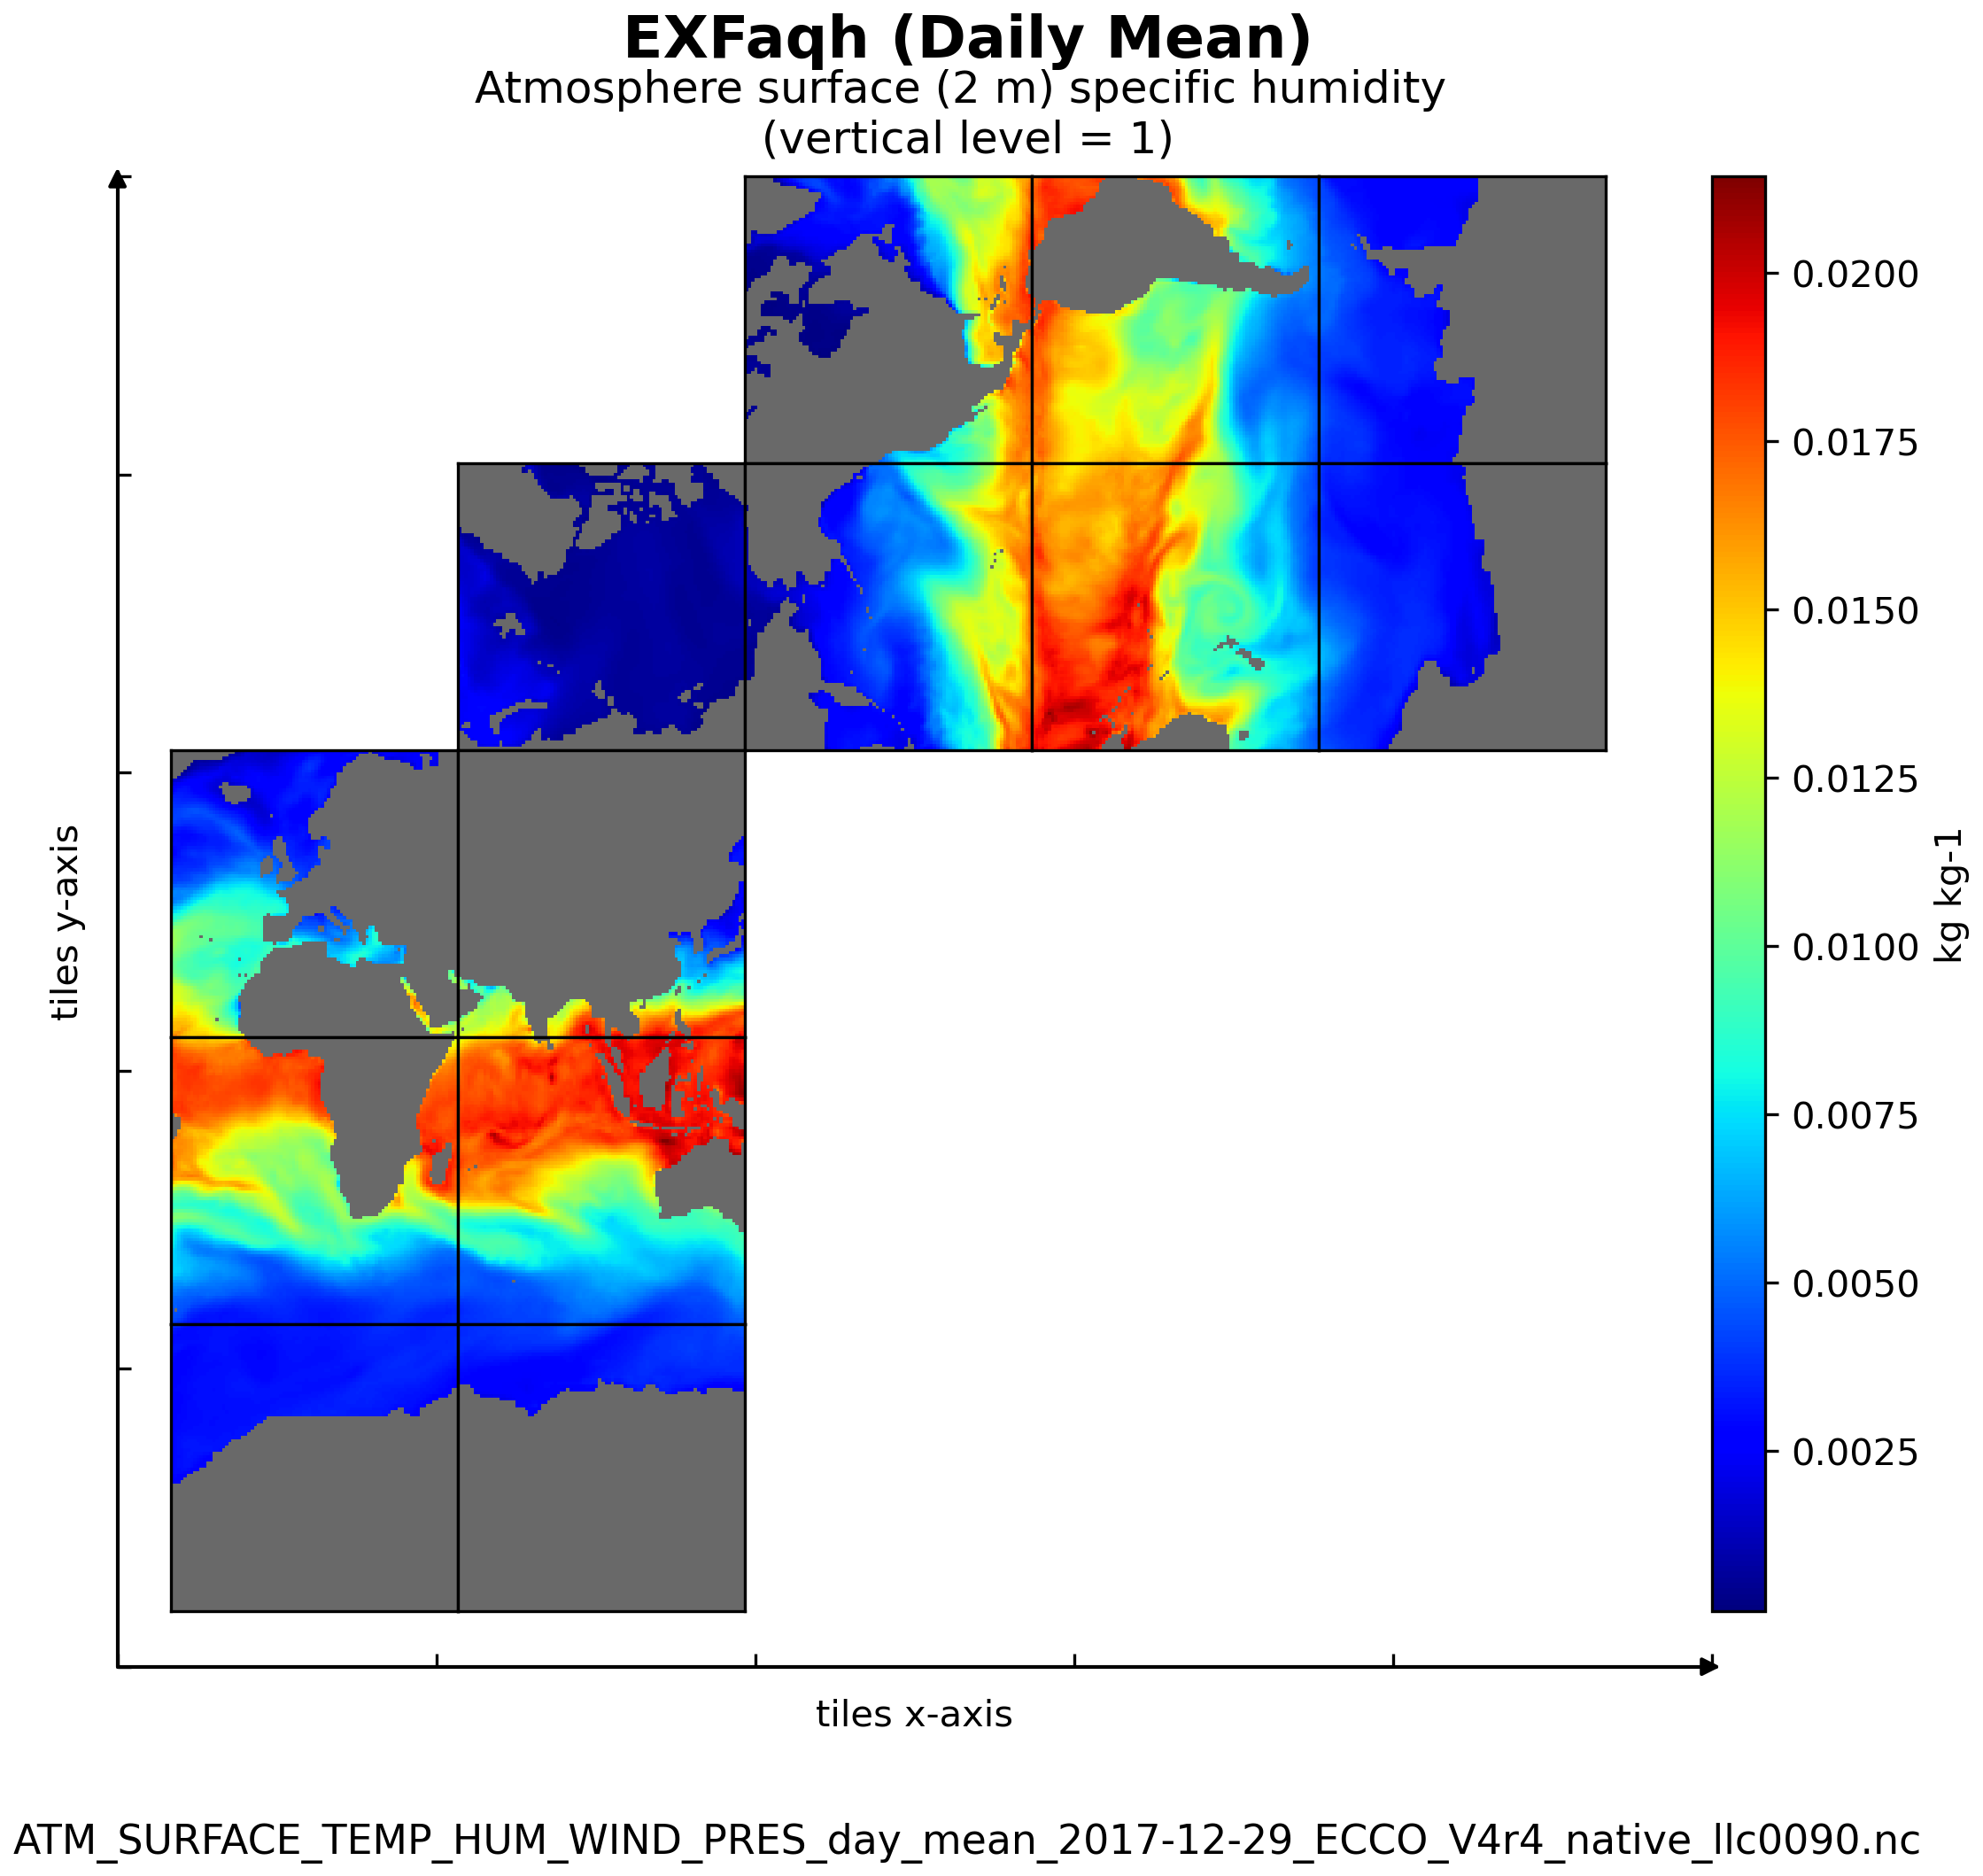
\includegraphics[scale=0.55]{../images/plots/v4r4/native_plots/Atmosphere_Surface_Temperature_Humidity_Wind_and_Pressure/EXFaqh.png}
\caption{Dataset: ATM\_SURFACE\_TEMP\_HUM\_WIND\_PRES, Variable: EXFaqh}
\label{tab:table-ATM_SURFACE_TEMP_HUM_WIND_PRES_EXFaqh-Plot}
\end{figure}
\newpage
\pagebreak
\subsubsection{Native Variable: EXFatemp}
\begin{longtable}{|m{0.06\textwidth}|m{0.3\textwidth}|m{0.45\textwidth}|m{0.12\textwidth}|}
\caption{Attributes description of the variable 'EXFatemp' from ATM\_SURFACE\_TEMP\_HUM\_WIND\_PRES's  dataset.}
\label{tab:table-ATM_SURFACE_TEMP_HUM_WIND_PRES_EXFatemp} \\ 
\hline \endhead \hline \endfoot
\rowcolor{lightgray} \textbf{Storage Type} & \textbf{Variable Name} & \textbf{Description} & \textbf{Unit} \\ \hline
float32 & EXFatemp & Atmosphere surface (2 m) air temperature  & degree\_K \\ \hline
\multicolumn{4}{|c|}{\cellcolor{lightgray}{\textbf{Description of the variable in Common Data language (CDL)}}} \\ \hline
\multicolumn{4}{|c|}{\fontfamily{lmtt}\selectfont{\makecell{\parbox{.95\textwidth}{\vspace*{0.25cm} \footnotesize{float32 EXFatemp(time, tile, j, i)\\
\hspace*{0.5cm}EXFatemp: \_FillValue = 9.96921e+36\\
\hspace*{0.5cm}EXFatemp: coordinates = time XC YC\\
\hspace*{0.5cm}EXFatemp: coverage\_content\_type = modelResult\\
\hspace*{0.5cm}EXFatemp: long\_name = Atmosphere surface (2 m) air temperature \\
\hspace*{0.5cm}EXFatemp: standard\_name = air temperature\\
\hspace*{0.5cm}EXFatemp: units = degree K\\
\hspace*{0.5cm}EXFatemp: valid\_max = 312.8451232910156\\
\hspace*{0.5cm}EXFatemp: valid\_min = 195.37054443359375\\
}}}}} \\ \hline
\rowcolor{lightgray} \multicolumn{4}{|c|}{\textbf{Comments}} \\ \hline
\multicolumn{4}{|p{1\textwidth}|}{\footnotesize{{Surface (2 m) air temperature over open water. note: sum of era-interim surface air temperature and the control adjustment from ocean state estimation.}}} \\ \hline
\end{longtable}

\begin{figure}[H]
\centering
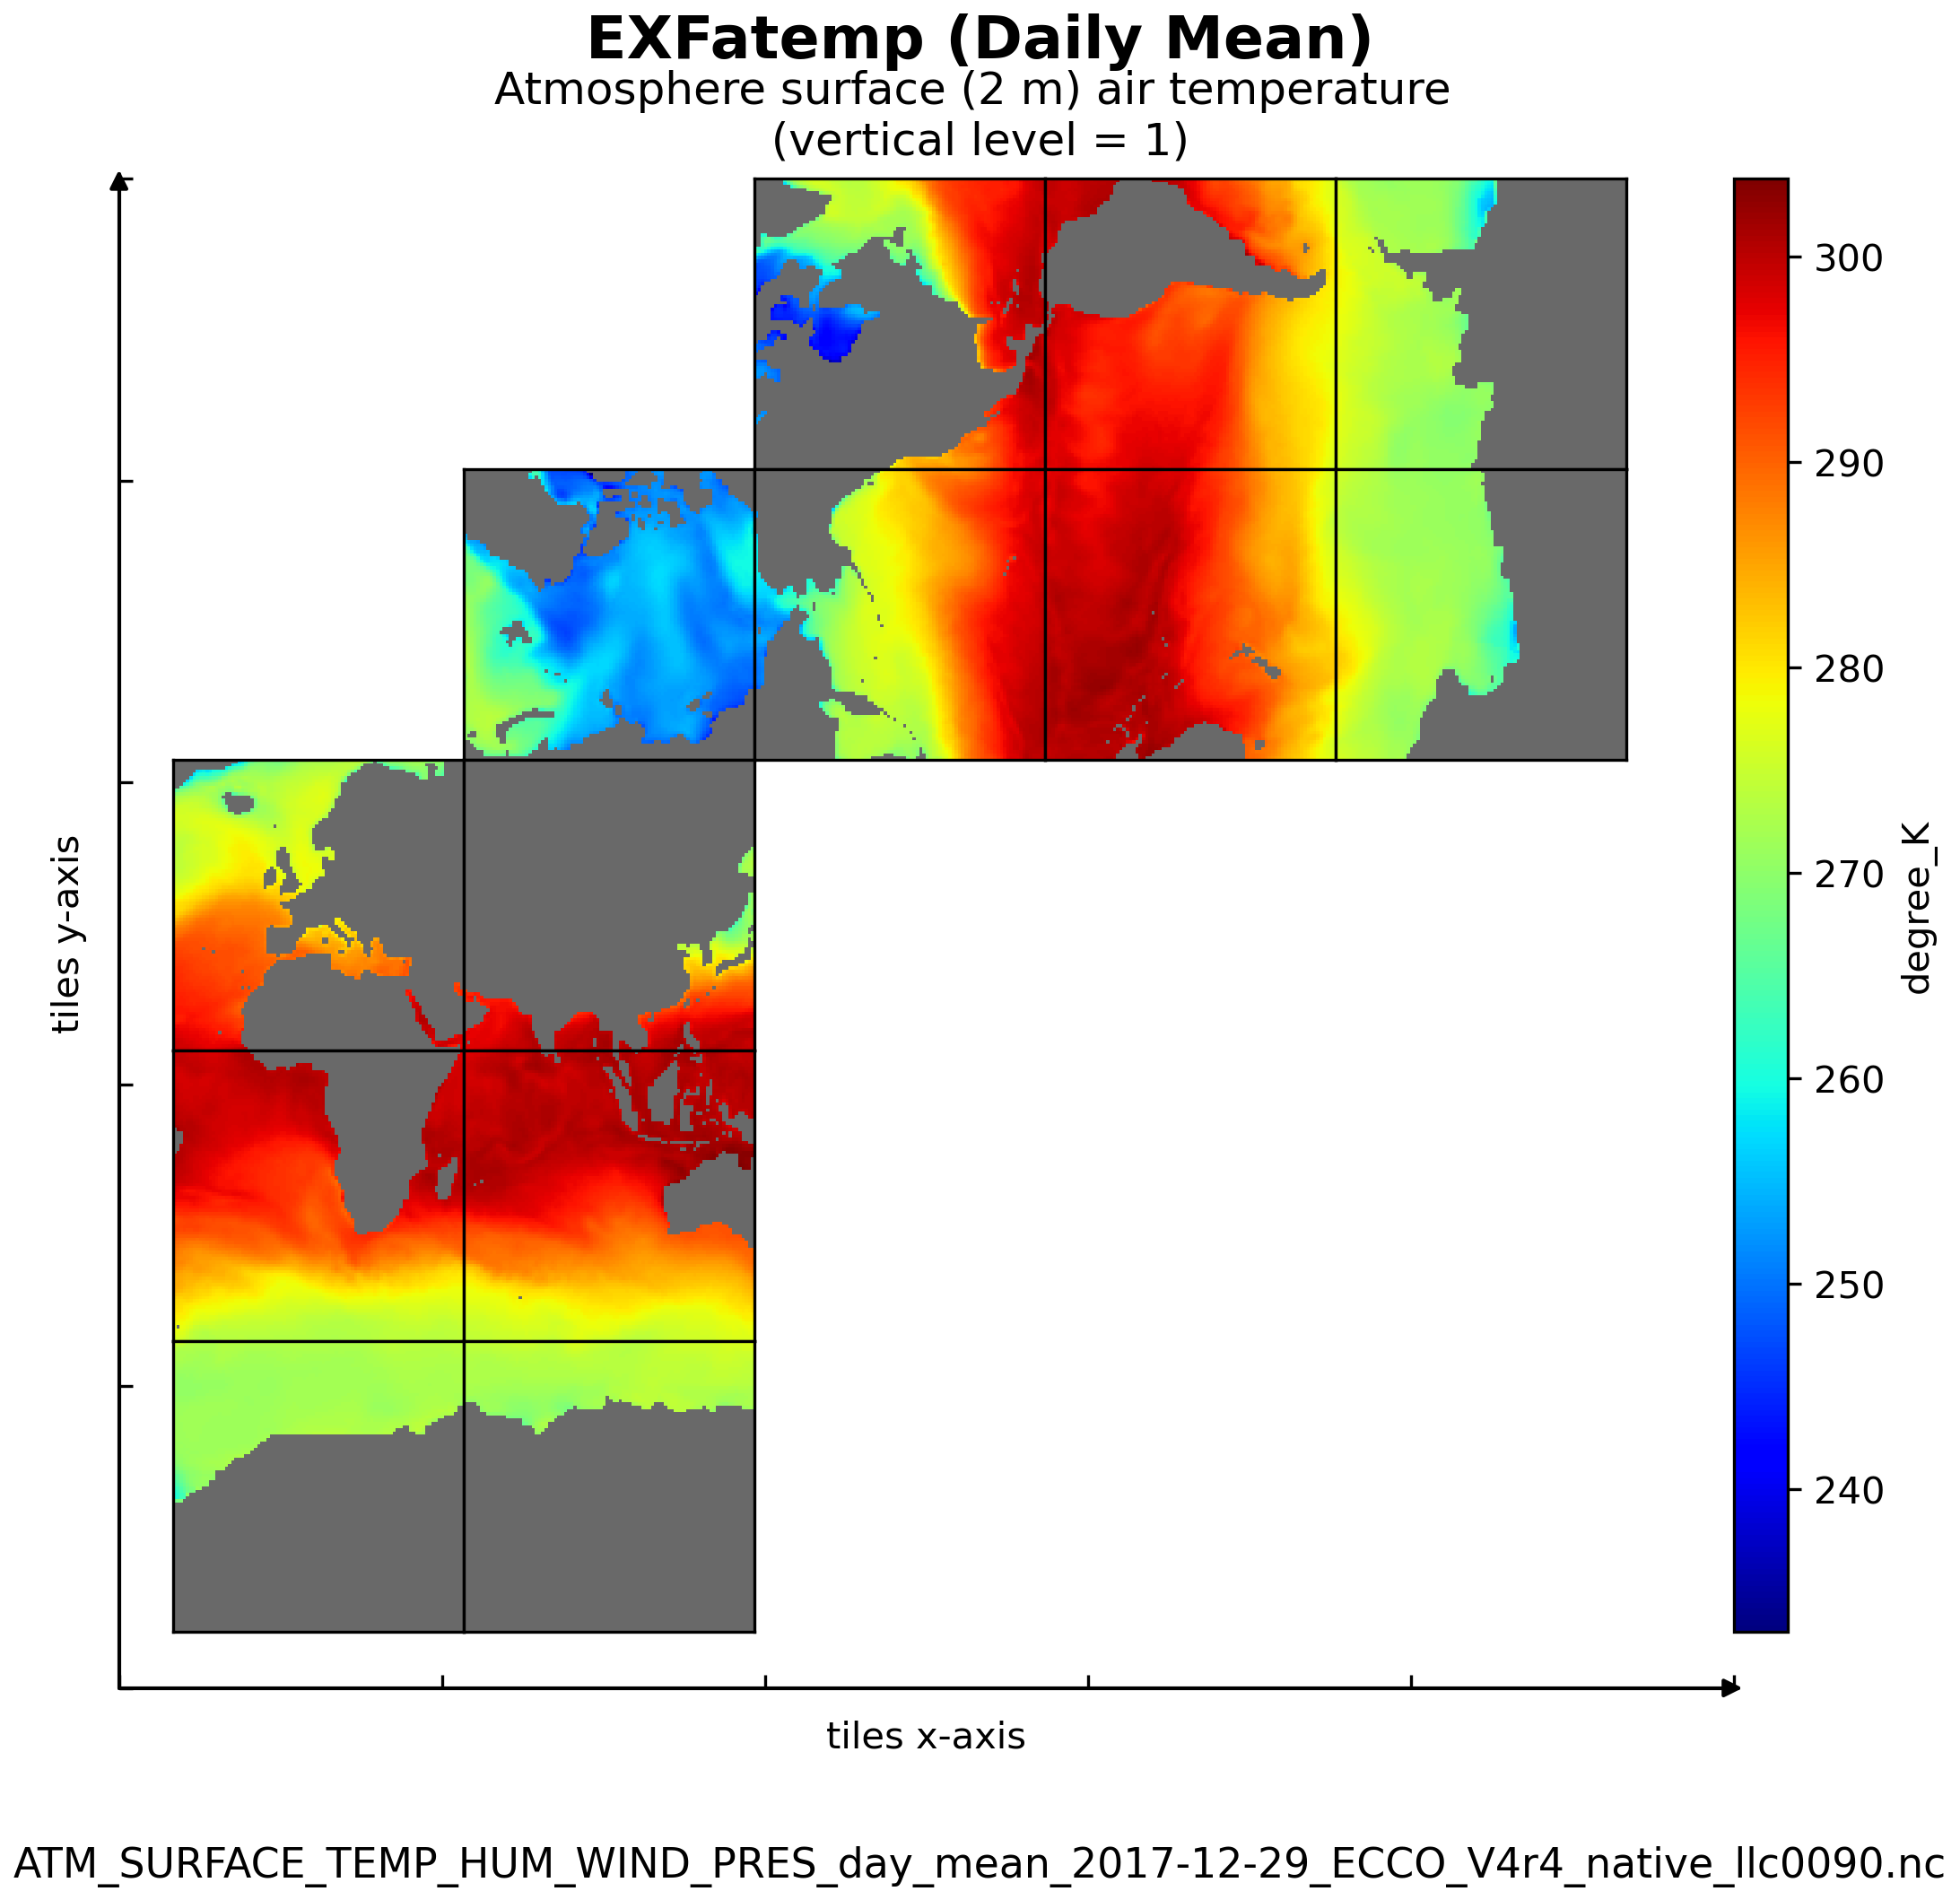
\includegraphics[scale=0.55]{../images/plots/v4r4/native_plots/Atmosphere_Surface_Temperature_Humidity_Wind_and_Pressure/EXFatemp.png}
\caption{Dataset: ATM\_SURFACE\_TEMP\_HUM\_WIND\_PRES, Variable: EXFatemp}
\label{tab:table-ATM_SURFACE_TEMP_HUM_WIND_PRES_EXFatemp-Plot}
\end{figure}
\newpage
\pagebreak
\subsubsection{Native Variable: EXFpress}
\begin{longtable}{|m{0.06\textwidth}|m{0.3\textwidth}|m{0.45\textwidth}|m{0.12\textwidth}|}
\caption{Attributes description of the variable 'EXFpress' from ATM\_SURFACE\_TEMP\_HUM\_WIND\_PRES's  dataset.}
\label{tab:table-ATM_SURFACE_TEMP_HUM_WIND_PRES_EXFpress} \\ 
\hline \endhead \hline \endfoot
\rowcolor{lightgray} \textbf{Storage Type} & \textbf{Variable Name} & \textbf{Description} & \textbf{Unit} \\ \hline
float32 & EXFpress & Atmosphere surface pressure & N m-2 \\ \hline
\multicolumn{4}{|c|}{\cellcolor{lightgray}{\textbf{Description of the variable in Common Data language (CDL)}}} \\ \hline
\multicolumn{4}{|c|}{\fontfamily{lmtt}\selectfont{\makecell{\parbox{.95\textwidth}{\vspace*{0.25cm} \footnotesize{float32 EXFpress(time, tile, j, i)\\
\hspace*{0.5cm}EXFpress: \_FillValue = 9.96921e+36\\
\hspace*{0.5cm}EXFpress: coordinates = time XC YC\\
\hspace*{0.5cm}EXFpress: coverage\_content\_type = modelResult\\
\hspace*{0.5cm}EXFpress: long\_name = Atmosphere surface pressure\\
\hspace*{0.5cm}EXFpress: standard\_name = surface air pressure\\
\hspace*{0.5cm}EXFpress: units = N m-2\\
\hspace*{0.5cm}EXFpress: valid\_max = 106314.7734375\\
\hspace*{0.5cm}EXFpress: valid\_min = 92044.171875\\
}}}}} \\ \hline
\rowcolor{lightgray} \multicolumn{4}{|c|}{\textbf{Comments}} \\ \hline
\multicolumn{4}{|p{1\textwidth}|}{\footnotesize{{Atmospheric pressure field at sea level. note: era-interim atmospheric pressure, with air tides removed using a variety of methods. not adjusted by the ocean state estimation.}}} \\ \hline
\end{longtable}

\begin{figure}[H]
\centering
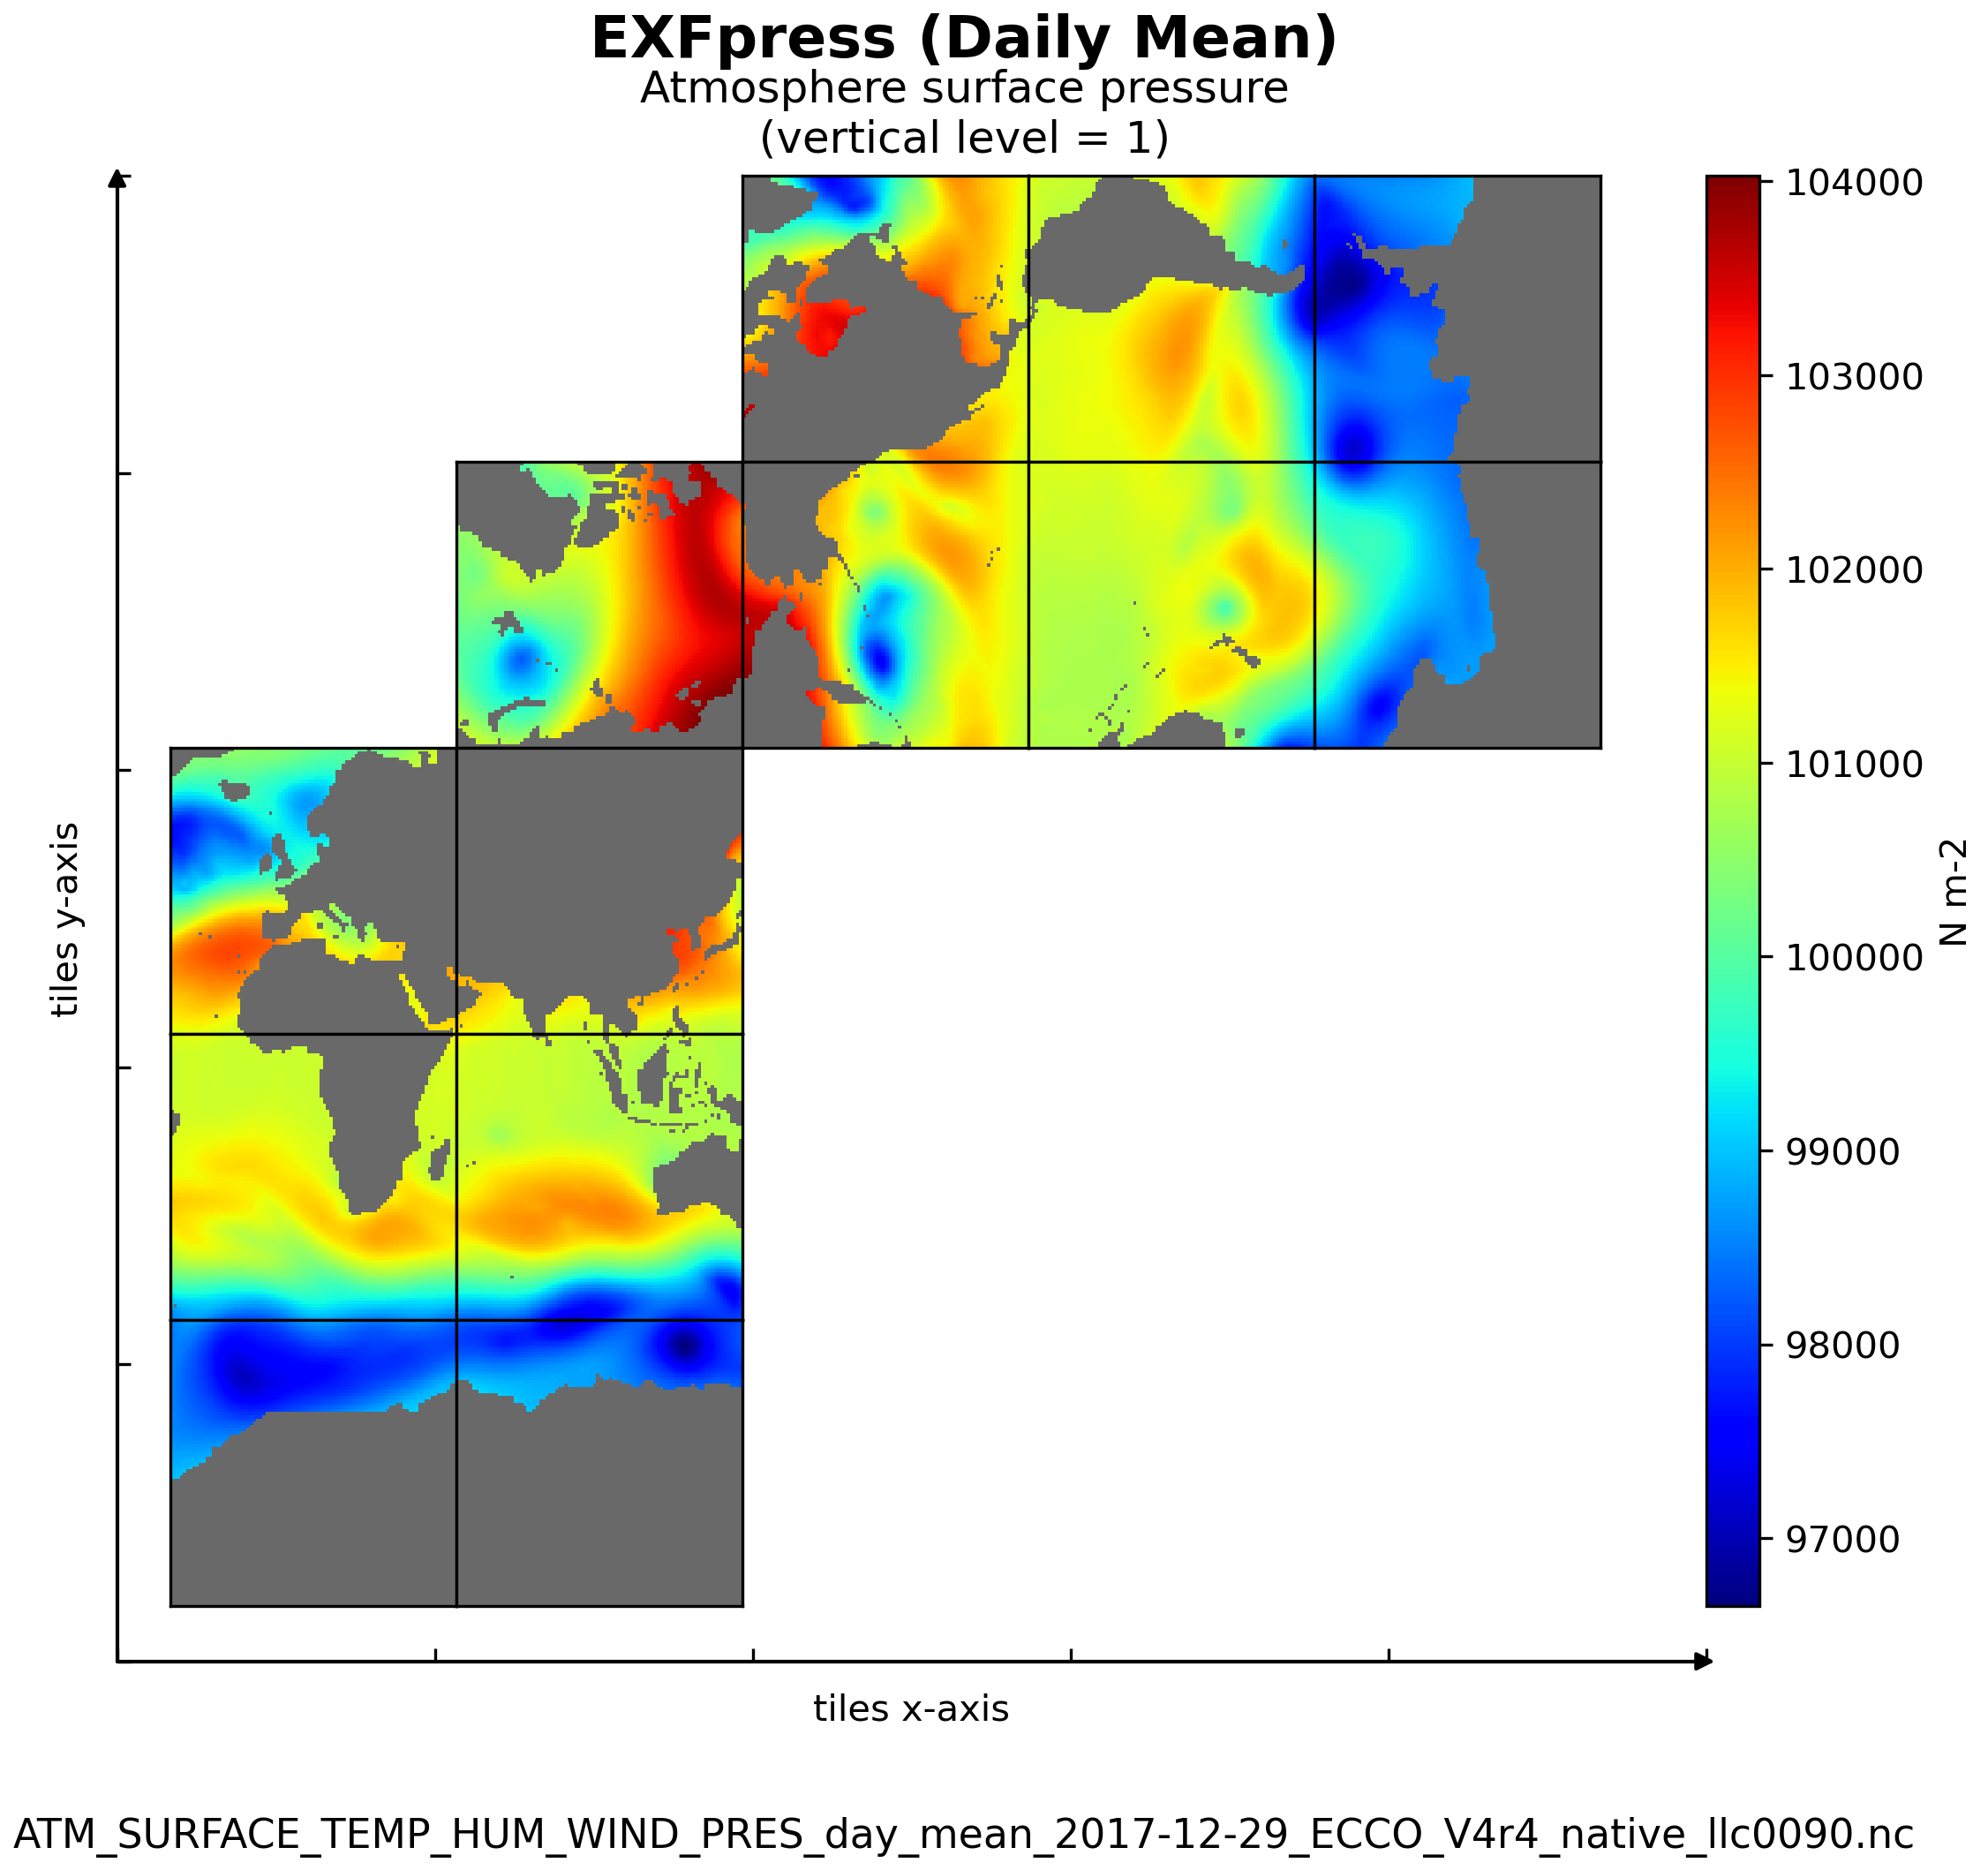
\includegraphics[scale=0.55]{../images/plots/v4r4/native_plots/Atmosphere_Surface_Temperature_Humidity_Wind_and_Pressure/EXFpress.png}
\caption{Dataset: ATM\_SURFACE\_TEMP\_HUM\_WIND\_PRES, Variable: EXFpress}
\label{tab:table-ATM_SURFACE_TEMP_HUM_WIND_PRES_EXFpress-Plot}
\end{figure}
\newpage
\pagebreak
\subsubsection{Native Variable: EXFuwind}
\begin{longtable}{|m{0.06\textwidth}|m{0.3\textwidth}|m{0.45\textwidth}|m{0.12\textwidth}|}
\caption{Attributes description of the variable 'EXFuwind' from ATM\_SURFACE\_TEMP\_HUM\_WIND\_PRES's  dataset.}
\label{tab:table-ATM_SURFACE_TEMP_HUM_WIND_PRES_EXFuwind} \\ 
\hline \endhead \hline \endfoot
\rowcolor{lightgray} \textbf{Storage Type} & \textbf{Variable Name} & \textbf{Description} & \textbf{Unit} \\ \hline
float32 & EXFuwind & Wind speed at 10m in the model +x direction & m s-1 \\ \hline
\multicolumn{4}{|c|}{\cellcolor{lightgray}{\textbf{Description of the variable in Common Data language (CDL)}}} \\ \hline
\multicolumn{4}{|c|}{\fontfamily{lmtt}\selectfont{\makecell{\parbox{.95\textwidth}{\vspace*{0.25cm} \footnotesize{float32 EXFuwind(time, tile, j, i)\\
\hspace*{0.5cm}EXFuwind: \_FillValue = 9.96921e+36\\
\hspace*{0.5cm}EXFuwind: coordinates = time XC YC\\
\hspace*{0.5cm}EXFuwind: coverage\_content\_type = modelResult\\
\hspace*{0.5cm}EXFuwind: long\_name = Wind speed at 10m in the model +x direction\\
\hspace*{0.5cm}EXFuwind: standard\_name = x wind\\
\hspace*{0.5cm}EXFuwind: units = m s-1\\
\hspace*{0.5cm}EXFuwind: valid\_max = 29.92486572265625\\
\hspace*{0.5cm}EXFuwind: valid\_min = -34.528900146484375\\
}}}}} \\ \hline
\rowcolor{lightgray} \multicolumn{4}{|c|}{\textbf{Comments}} \\ \hline
\multicolumn{4}{|p{1\textwidth}|}{\footnotesize{{Wind speed at 10m in the +x direction at the tracer cell on the native model grid. note: ecco v4r4 is forced with wind stress (see exftaux) not vector winds converted to wind stress using bulk formulae. exfuwind is calculated by converting wind stress to vector wind using bulk formulae.}}} \\ \hline
\end{longtable}

\begin{figure}[H]
\centering
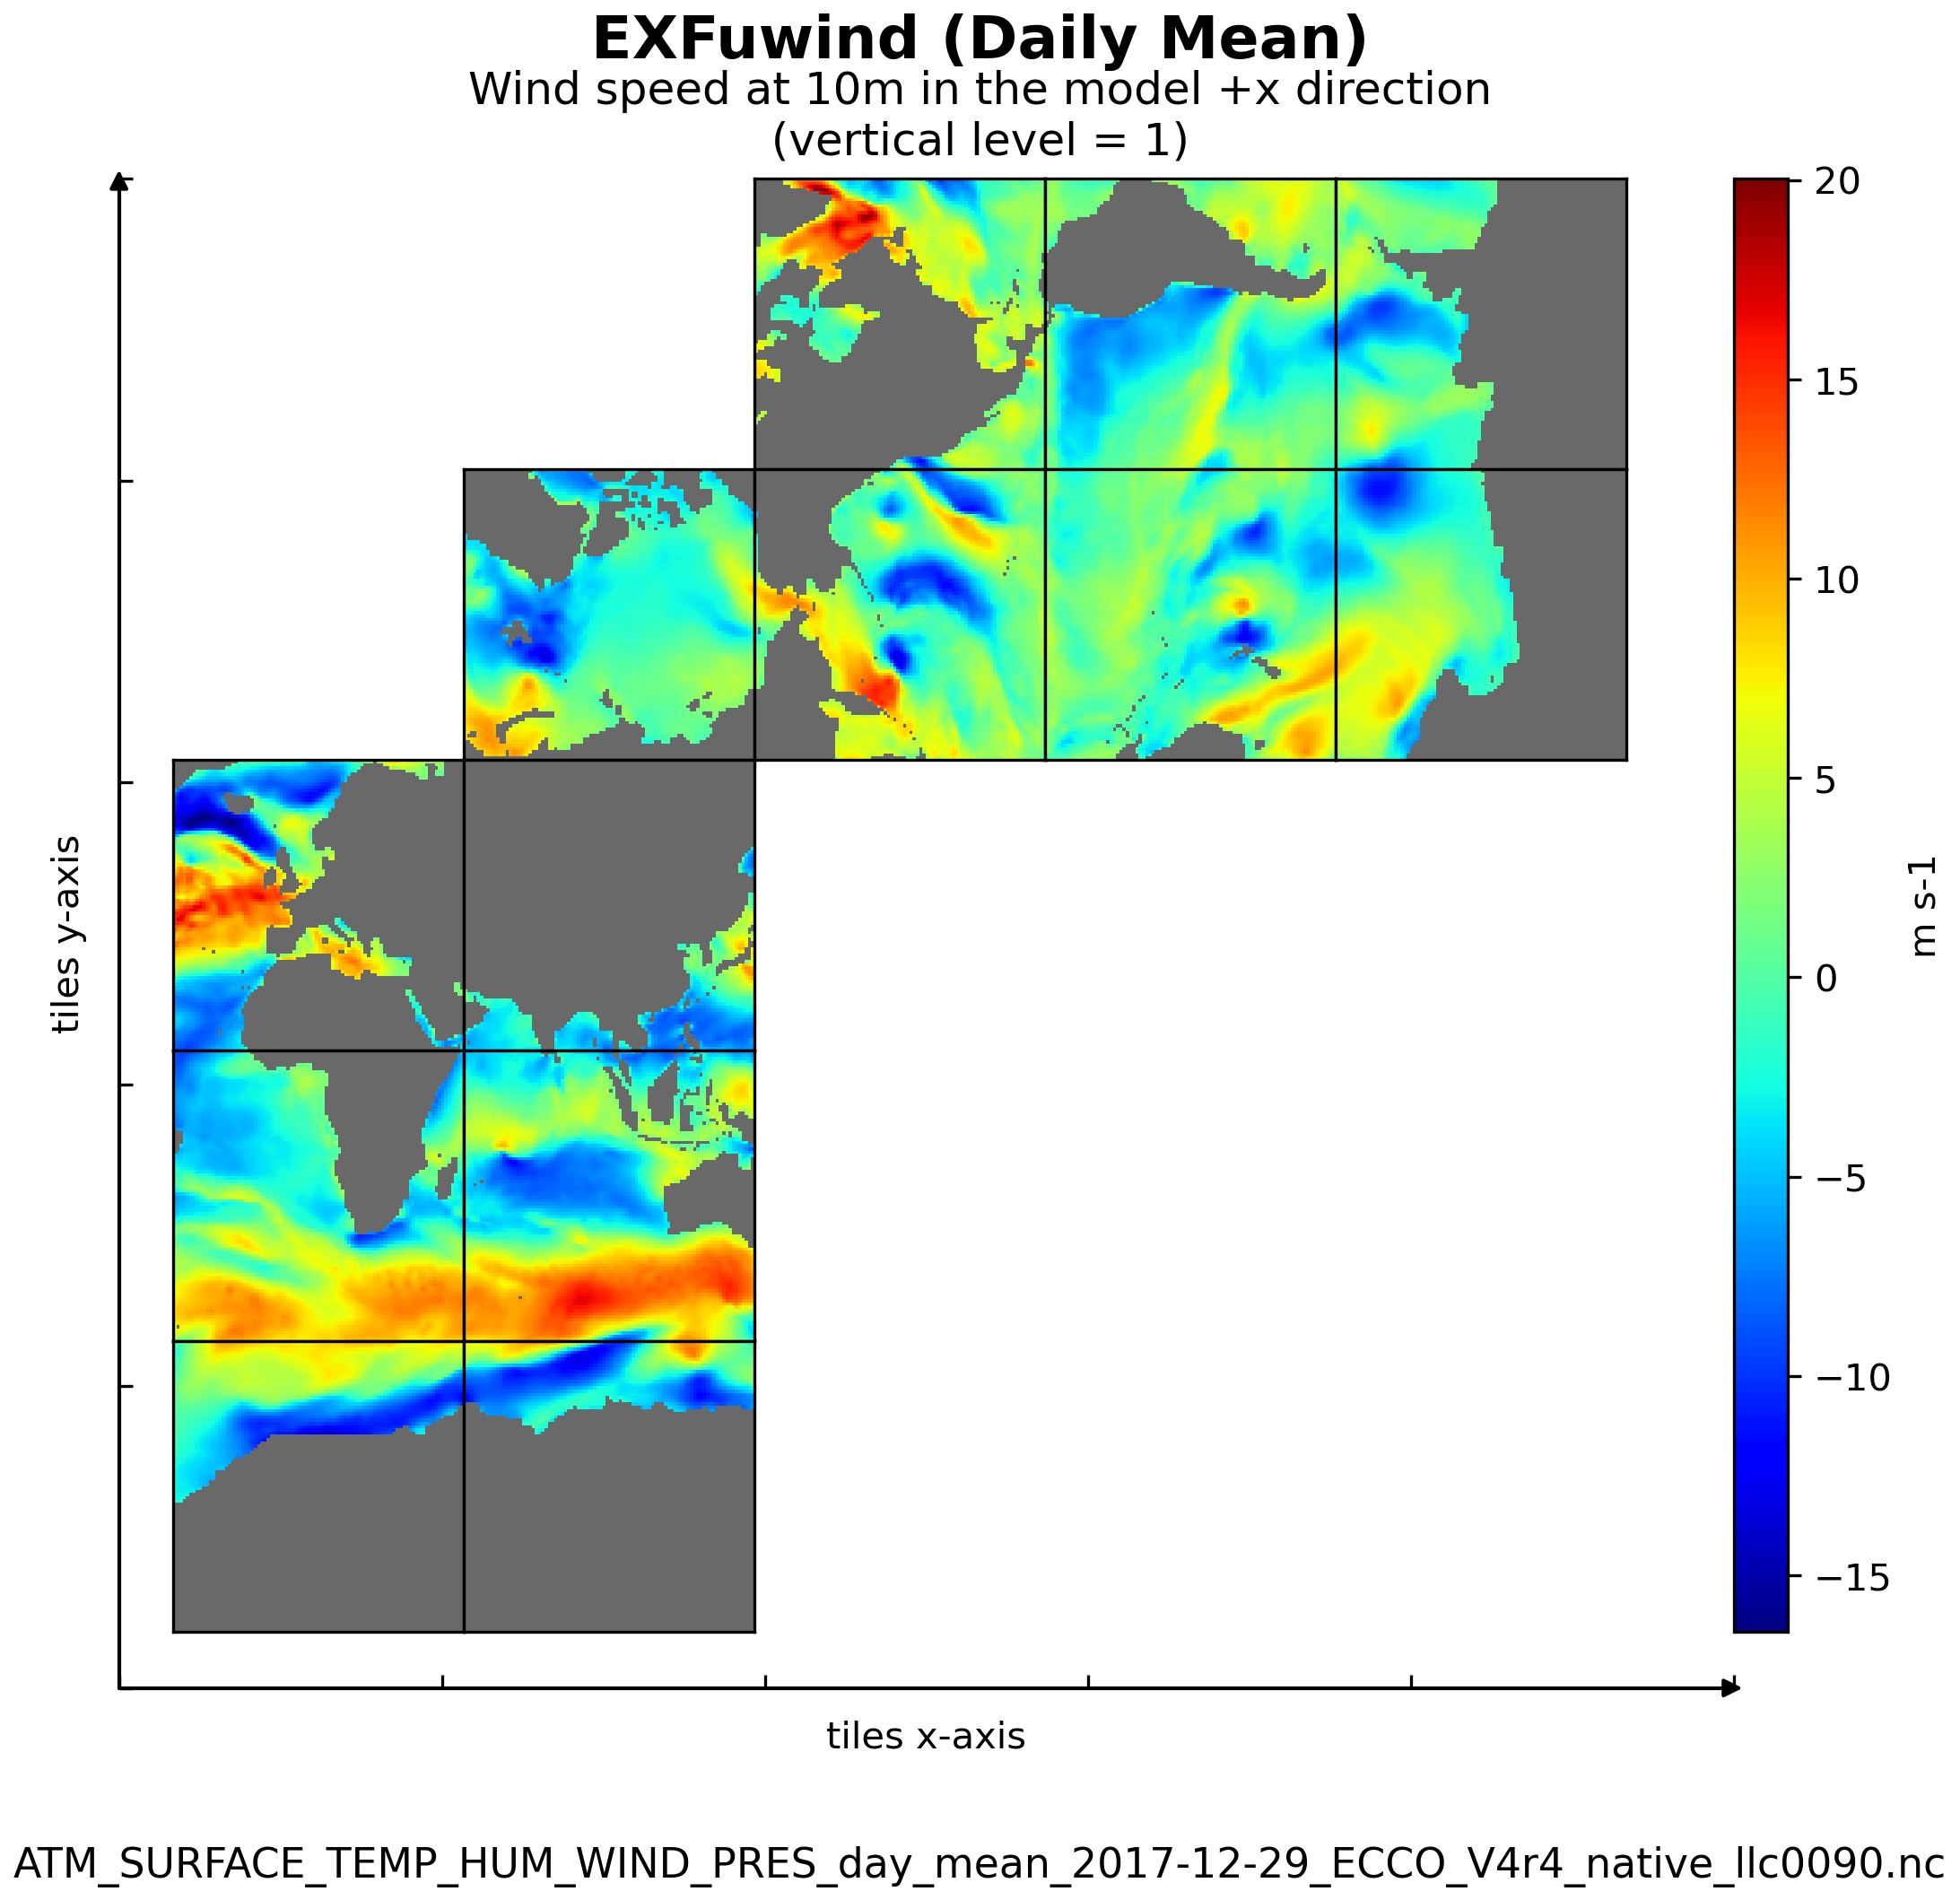
\includegraphics[scale=0.55]{../images/plots/v4r4/native_plots/Atmosphere_Surface_Temperature_Humidity_Wind_and_Pressure/EXFuwind.png}
\caption{Dataset: ATM\_SURFACE\_TEMP\_HUM\_WIND\_PRES, Variable: EXFuwind}
\label{tab:table-ATM_SURFACE_TEMP_HUM_WIND_PRES_EXFuwind-Plot}
\end{figure}
\newpage
\pagebreak
\subsubsection{Native Variable: EXFvwind}
\begin{longtable}{|m{0.06\textwidth}|m{0.3\textwidth}|m{0.45\textwidth}|m{0.12\textwidth}|}
\caption{Attributes description of the variable 'EXFvwind' from ATM\_SURFACE\_TEMP\_HUM\_WIND\_PRES's  dataset.}
\label{tab:table-ATM_SURFACE_TEMP_HUM_WIND_PRES_EXFvwind} \\ 
\hline \endhead \hline \endfoot
\rowcolor{lightgray} \textbf{Storage Type} & \textbf{Variable Name} & \textbf{Description} & \textbf{Unit} \\ \hline
float32 & EXFvwind & Wind speed at 10m in the model +y direction & m s-1 \\ \hline
\multicolumn{4}{|c|}{\cellcolor{lightgray}{\textbf{Description of the variable in Common Data language (CDL)}}} \\ \hline
\multicolumn{4}{|c|}{\fontfamily{lmtt}\selectfont{\makecell{\parbox{.95\textwidth}{\vspace*{0.25cm} \footnotesize{float32 EXFvwind(time, tile, j, i)\\
\hspace*{0.5cm}EXFvwind: \_FillValue = 9.96921e+36\\
\hspace*{0.5cm}EXFvwind: coordinates = time XC YC\\
\hspace*{0.5cm}EXFvwind: coverage\_content\_type = modelResult\\
\hspace*{0.5cm}EXFvwind: long\_name = Wind speed at 10m in the model +y direction\\
\hspace*{0.5cm}EXFvwind: standard\_name = y wind\\
\hspace*{0.5cm}EXFvwind: units = m s-1\\
\hspace*{0.5cm}EXFvwind: valid\_max = 45.065101623535156\\
\hspace*{0.5cm}EXFvwind: valid\_min = -27.9254093170166\\
}}}}} \\ \hline
\rowcolor{lightgray} \multicolumn{4}{|c|}{\textbf{Comments}} \\ \hline
\multicolumn{4}{|p{1\textwidth}|}{\footnotesize{{Wind speed at 10m in the +y direction at the tracer cell on the native model grid. note: ecco v4r4 is forced with wind stress (see exftauy) not vector winds converted to wind stress using bulk formulae. exfvwind is calculated by converting wind stress to vector wind using bulk formulae.}}} \\ \hline
\end{longtable}

\begin{figure}[H]
\centering
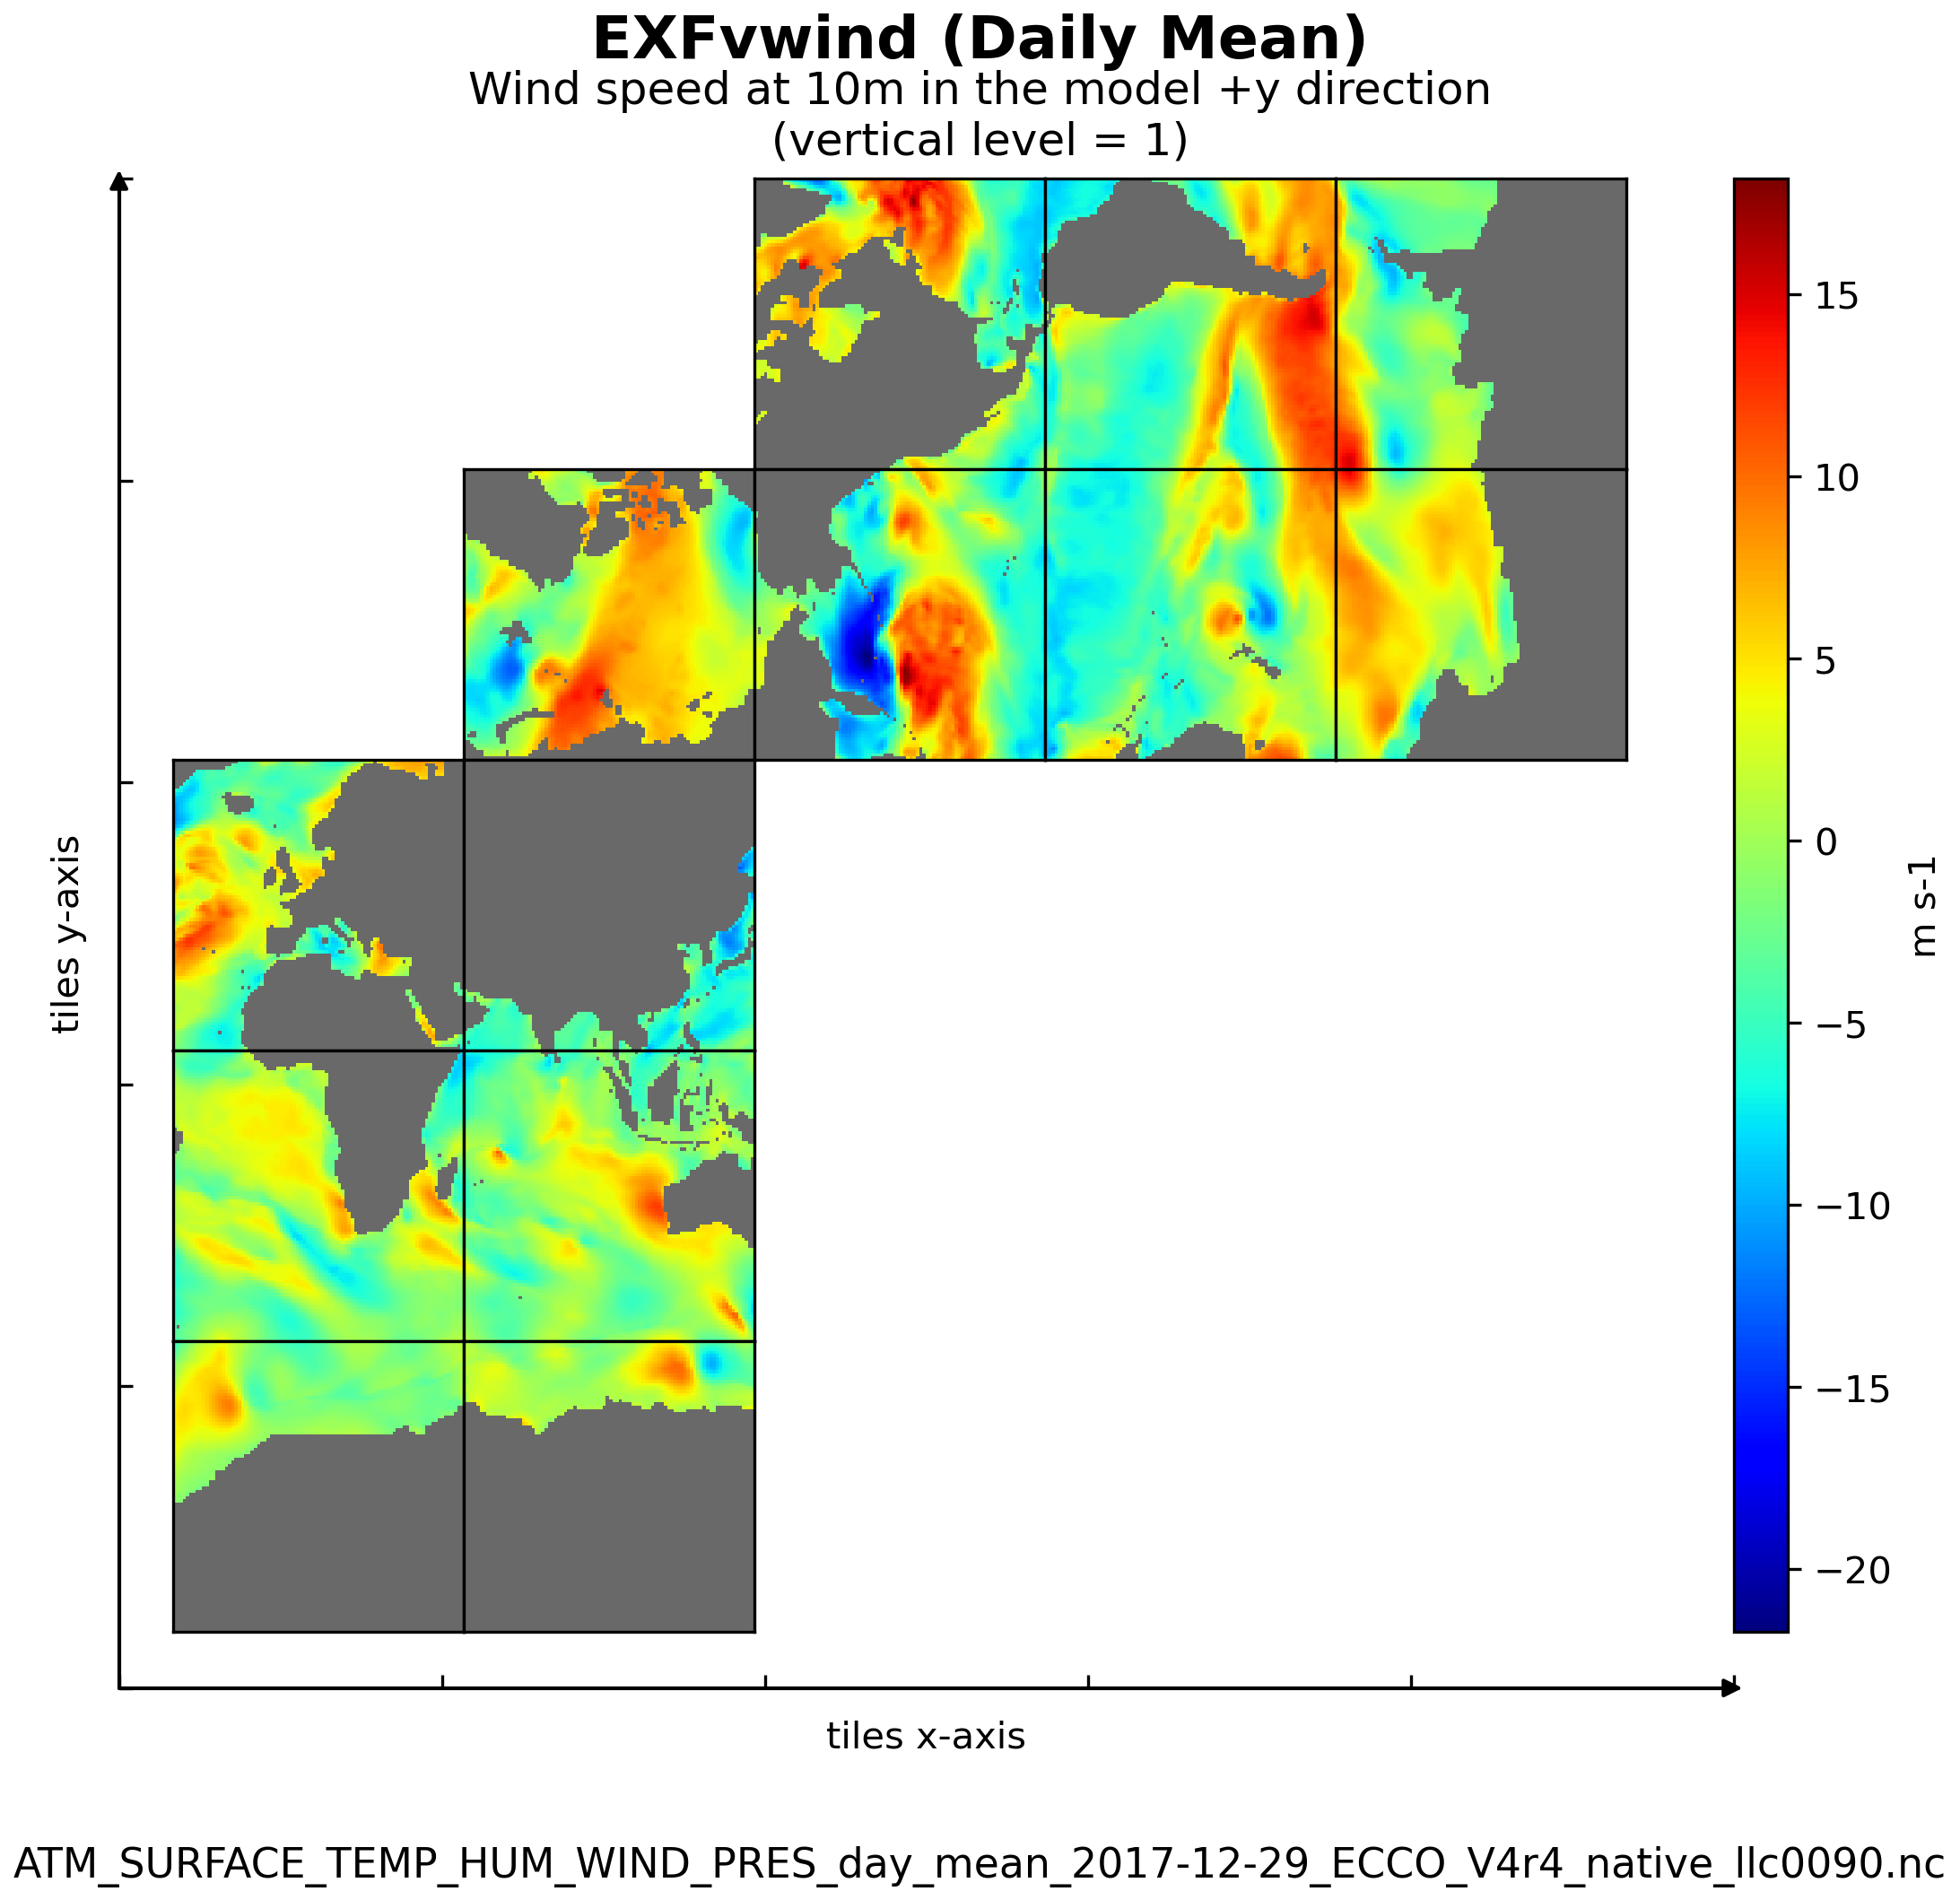
\includegraphics[scale=0.55]{../images/plots/v4r4/native_plots/Atmosphere_Surface_Temperature_Humidity_Wind_and_Pressure/EXFvwind.png}
\caption{Dataset: ATM\_SURFACE\_TEMP\_HUM\_WIND\_PRES, Variable: EXFvwind}
\label{tab:table-ATM_SURFACE_TEMP_HUM_WIND_PRES_EXFvwind-Plot}
\end{figure}
\newpage
\pagebreak
\subsubsection{Native Variable: EXFwspee}
\begin{longtable}{|m{0.06\textwidth}|m{0.3\textwidth}|m{0.45\textwidth}|m{0.12\textwidth}|}
\caption{Attributes description of the variable 'EXFwspee' from ATM\_SURFACE\_TEMP\_HUM\_WIND\_PRES's  dataset.}
\label{tab:table-ATM_SURFACE_TEMP_HUM_WIND_PRES_EXFwspee} \\ 
\hline \endhead \hline \endfoot
\rowcolor{lightgray} \textbf{Storage Type} & \textbf{Variable Name} & \textbf{Description} & \textbf{Unit} \\ \hline
float32 & EXFwspee & Wind speed & m s-1 \\ \hline
\multicolumn{4}{|c|}{\cellcolor{lightgray}{\textbf{Description of the variable in Common Data language (CDL)}}} \\ \hline
\multicolumn{4}{|c|}{\fontfamily{lmtt}\selectfont{\makecell{\parbox{.95\textwidth}{\vspace*{0.25cm} \footnotesize{float32 EXFwspee(time, tile, j, i)\\
\hspace*{0.5cm}EXFwspee: \_FillValue = 9.96921e+36\\
\hspace*{0.5cm}EXFwspee: coordinates = time XC YC\\
\hspace*{0.5cm}EXFwspee: coverage\_content\_type = modelResult\\
\hspace*{0.5cm}EXFwspee: long\_name = Wind speed\\
\hspace*{0.5cm}EXFwspee: standard\_name = wind speed\\
\hspace*{0.5cm}EXFwspee: units = m s-1\\
\hspace*{0.5cm}EXFwspee: valid\_max = 45.87086486816406\\
\hspace*{0.5cm}EXFwspee: valid\_min = 0.27271032333374023\\
}}}}} \\ \hline
\rowcolor{lightgray} \multicolumn{4}{|c|}{\textbf{Comments}} \\ \hline
\multicolumn{4}{|p{1\textwidth}|}{\footnotesize{{10-m wind speed magnitude (>= 0 ) over open water. only used for the calculation of air-sea fluxes using bulk formulae. note: not adjusted by the ocean state estimation and not necesarily consistent with exfuwind and exfvwind because exfuwind and exfvwind are calculated from exftaux and exftauy using bulk formulae. exfwspee != sqrt(exfuwind**2 + exfvwind**2.}}} \\ \hline
\end{longtable}

\begin{figure}[H]
\centering
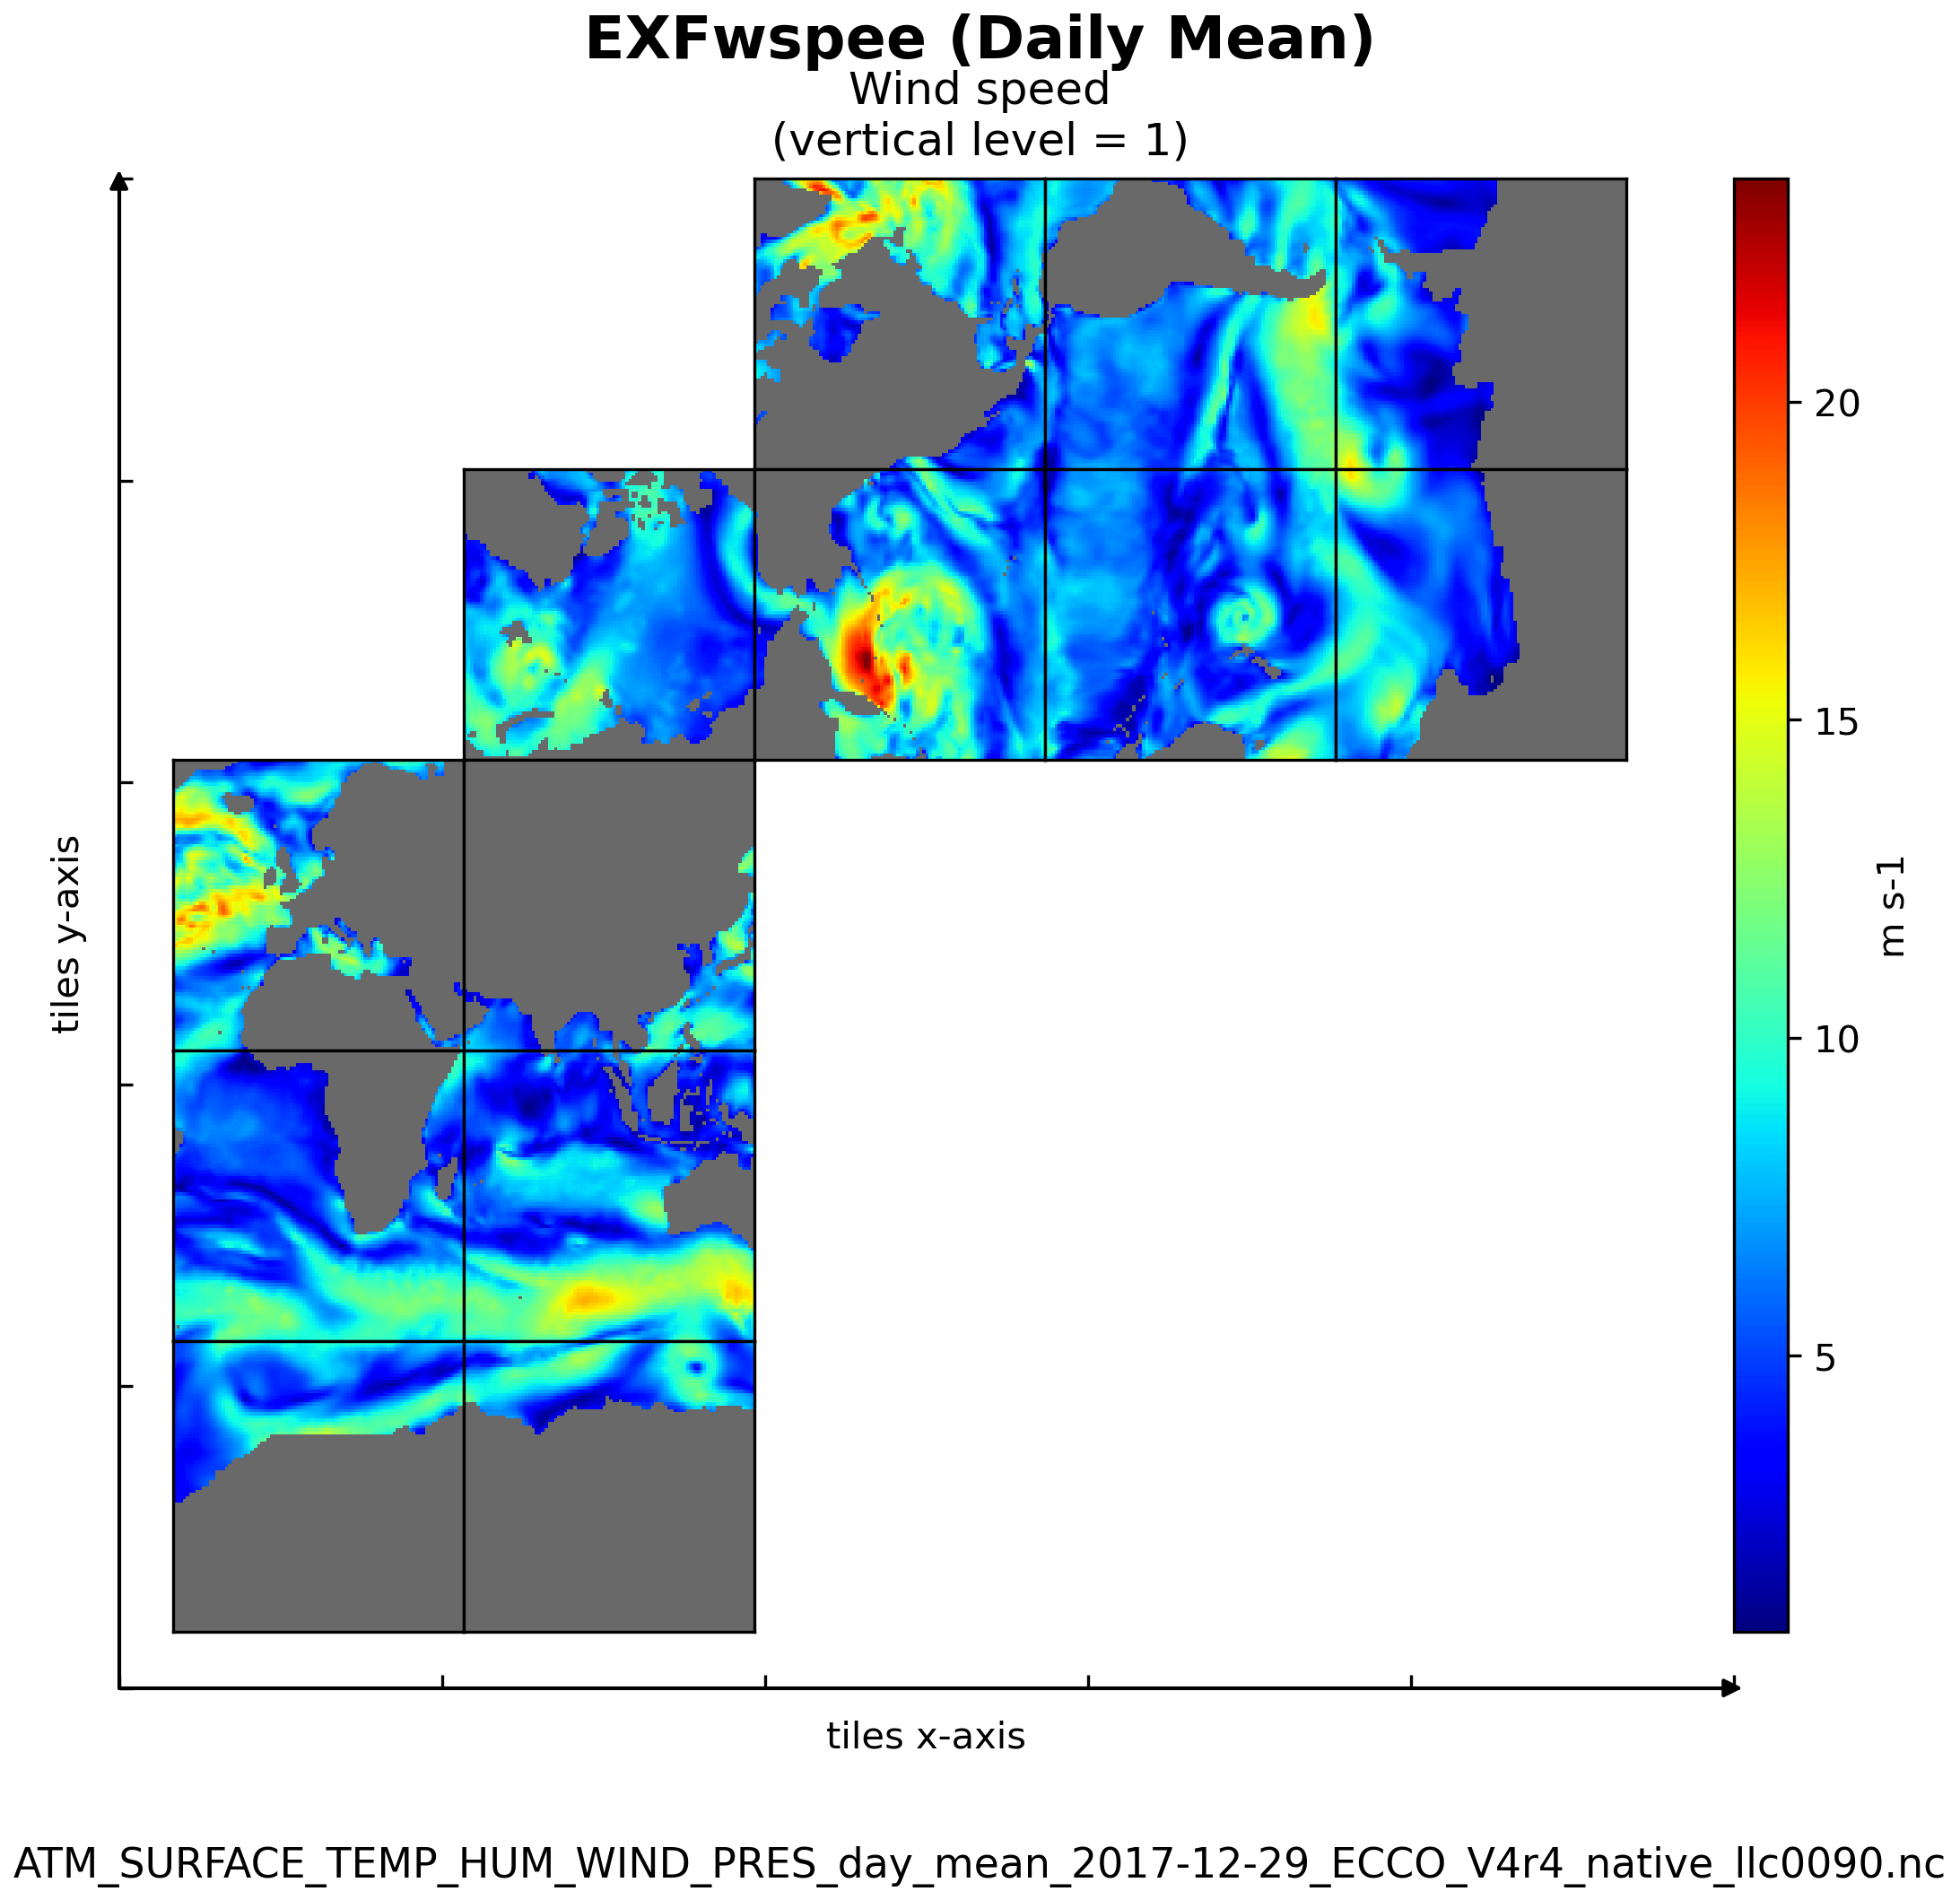
\includegraphics[scale=0.55]{../images/plots/v4r4/native_plots/Atmosphere_Surface_Temperature_Humidity_Wind_and_Pressure/EXFwspee.png}
\caption{Dataset: ATM\_SURFACE\_TEMP\_HUM\_WIND\_PRES, Variable: EXFwspee}
\label{tab:table-ATM_SURFACE_TEMP_HUM_WIND_PRES_EXFwspee-Plot}
\end{figure}
\newpage
\subsection{Native dataset of OCEAN\_3D\_MIXING\_COEFFS}
\newp
\subsubsection{Overview}
This dataset provides 3D time-invariant coefficients for the Gent-McWilliams and Redi parameterizations and background vertical diffusivity on the lat-lon-cap 90 (llc90) native model grid from the ECCO Version 4 Release 4 (V4r4) ocean and sea-ice state estimate. 
\begin{longtable}{|m{0.15\textwidth}|m{0.64\textwidth}|m{0.12\textwidth}|}
\caption{Coordinates and Variables in the dataset OCEAN\_3D\_MIXING\_COEFFS\_ECCO}
\label{tab:table-OCEAN_3D_MIXING_COEFFS_ECCO-fields} \\ 
\hline \endhead \hline \endfoot
\rowcolor{lightgray} \multicolumn{1}{|c|}{\textbf{Coordinates}} & \multicolumn{1}{|c|}{\textbf{Description of data coordinates}} &  \multicolumn{1}{|c|}{\textbf{Unit}}\\ \hline
i &Grid index in x for variables at tracer and 'v' locations &--none--  \\ \hline
i\_g &Grid index in x for variables at 'u' and 'g' locations &--none--  \\ \hline
j &Grid index in y for variables at tracer and 'u' locations &--none--  \\ \hline
j\_g &Grid index in y for variables at 'v' and 'g' locations &--none--  \\ \hline
k &Grid index in z for tracer variables &--none--  \\ \hline
k\_u &Grid index in z corresponding to the bottom face of tracer grid cells ('w' locations) &--none--  \\ \hline
k\_l &Grid index in z corresponding to the top face of tracer grid cells ('w' locations) &--none--  \\ \hline
k\_p1 &Grid index in z for variables at 'w' locations &--none--  \\ \hline
tile &Lat-lon-cap tile index &--none--  \\ \hline
XC &Longitude of tracer grid cell center &degrees\_east  \\ \hline
YC &Latitude of tracer grid cell center &degrees\_north  \\ \hline
XG &Longitude of 'southwest' corner of tracer grid cell &degrees\_east  \\ \hline
YG &Latitude of 'southwest' corner of tracer grid cell &degrees\_north  \\ \hline
Z &Depth of tracer grid cell center &m  \\ \hline
Zp1 &Depth of top/bottom face of tracer grid cell &m  \\ \hline
Zu &Depth of bottom face of tracer grid cell &m  \\ \hline
Zl &Depth of top face of tracer grid cell &m  \\ \hline
XC\_bnds &Longitudes of tracer grid cell corners &--none--  \\ \hline
YC\_bnds &Latitudes of tracer grid cell corners &--none--  \\ \hline
Z\_bnds &Depths of top and bottom faces of tracer grid cell &--none--  \\ \hline
\rowcolor{lightgray} \multicolumn{1}{|c|}{\textbf{Variables}} & \multicolumn{1}{|c|}{\textbf{Description of data variables}} &  \multicolumn{1}{|c|}{\textbf{Unit}}\\ \hline
DIFFKR &Vertical diffusivity &m2 s-1  \\ \hline
KAPGM &Gent-mcwilliams diffusivity &m2 s-1  \\ \hline
KAPREDI &Along-isopycnal diffusivity &m2 s-1  \\ \hline
\end{longtable}

\newp
\pagebreak
\subsubsection{Native Variable: DIFFKR}
\begin{longtable}{|m{0.06\textwidth}|m{0.3\textwidth}|m{0.45\textwidth}|m{0.12\textwidth}|}
\caption{Attributes description of the variable 'DIFFKR' from OCEAN\_3D\_MIXING\_COEFFS's  dataset.}
\label{tab:table-OCEAN_3D_MIXING_COEFFS_DIFFKR} \\ 
\hline \endhead \hline \endfoot
\rowcolor{lightgray} \textbf{Storage Type} & \textbf{Variable Name} & \textbf{Description} & \textbf{Unit} \\ \hline
float32 & DIFFKR & Vertical diffusivity & m2 s-1 \\ \hline
\multicolumn{4}{|c|}{\cellcolor{lightgray}{\textbf{Description of the variable in Common Data language (CDL)}}} \\ \hline
\multicolumn{4}{|c|}{\fontfamily{lmtt}\selectfont{\makecell{\parbox{.95\textwidth}{\vspace*{0.25cm} \footnotesize{float32 DIFFKR(k, tile, j, i)\\
\hspace*{0.5cm}DIFFKR: \_FillValue = 9.96921e+36\\
\hspace*{0.5cm}DIFFKR: coordinates = Z XC YC\\
\hspace*{0.5cm}DIFFKR: coverage\_content\_type = modelResult\\
\hspace*{0.5cm}DIFFKR: long\_name = Vertical diffusivity\\
\hspace*{0.5cm}DIFFKR: units = m2 s-1\\
\hspace*{0.5cm}DIFFKR: valid\_max = 0.0001854995\\
\hspace*{0.5cm}DIFFKR: valid\_min = 1e-06\\
}}}}} \\ \hline
\rowcolor{lightgray} \multicolumn{4}{|c|}{\textbf{Comments}} \\ \hline
\multicolumn{4}{|p{1\textwidth}|}{\footnotesize{{Background vertical diffusion coefficient for temperature and salinity. total vertical diffusivity includes background diffusivity plus contributions from the ggl90 vertical mixing and the gent-mcwilliams/redi parameterizations. note: diffkr is a model control variable and has been optimized from a spatially-invariant first-guess value of 1e-5 m2 s-1.}}} \\ \hline
\end{longtable}

\begin{figure}[H]
\centering
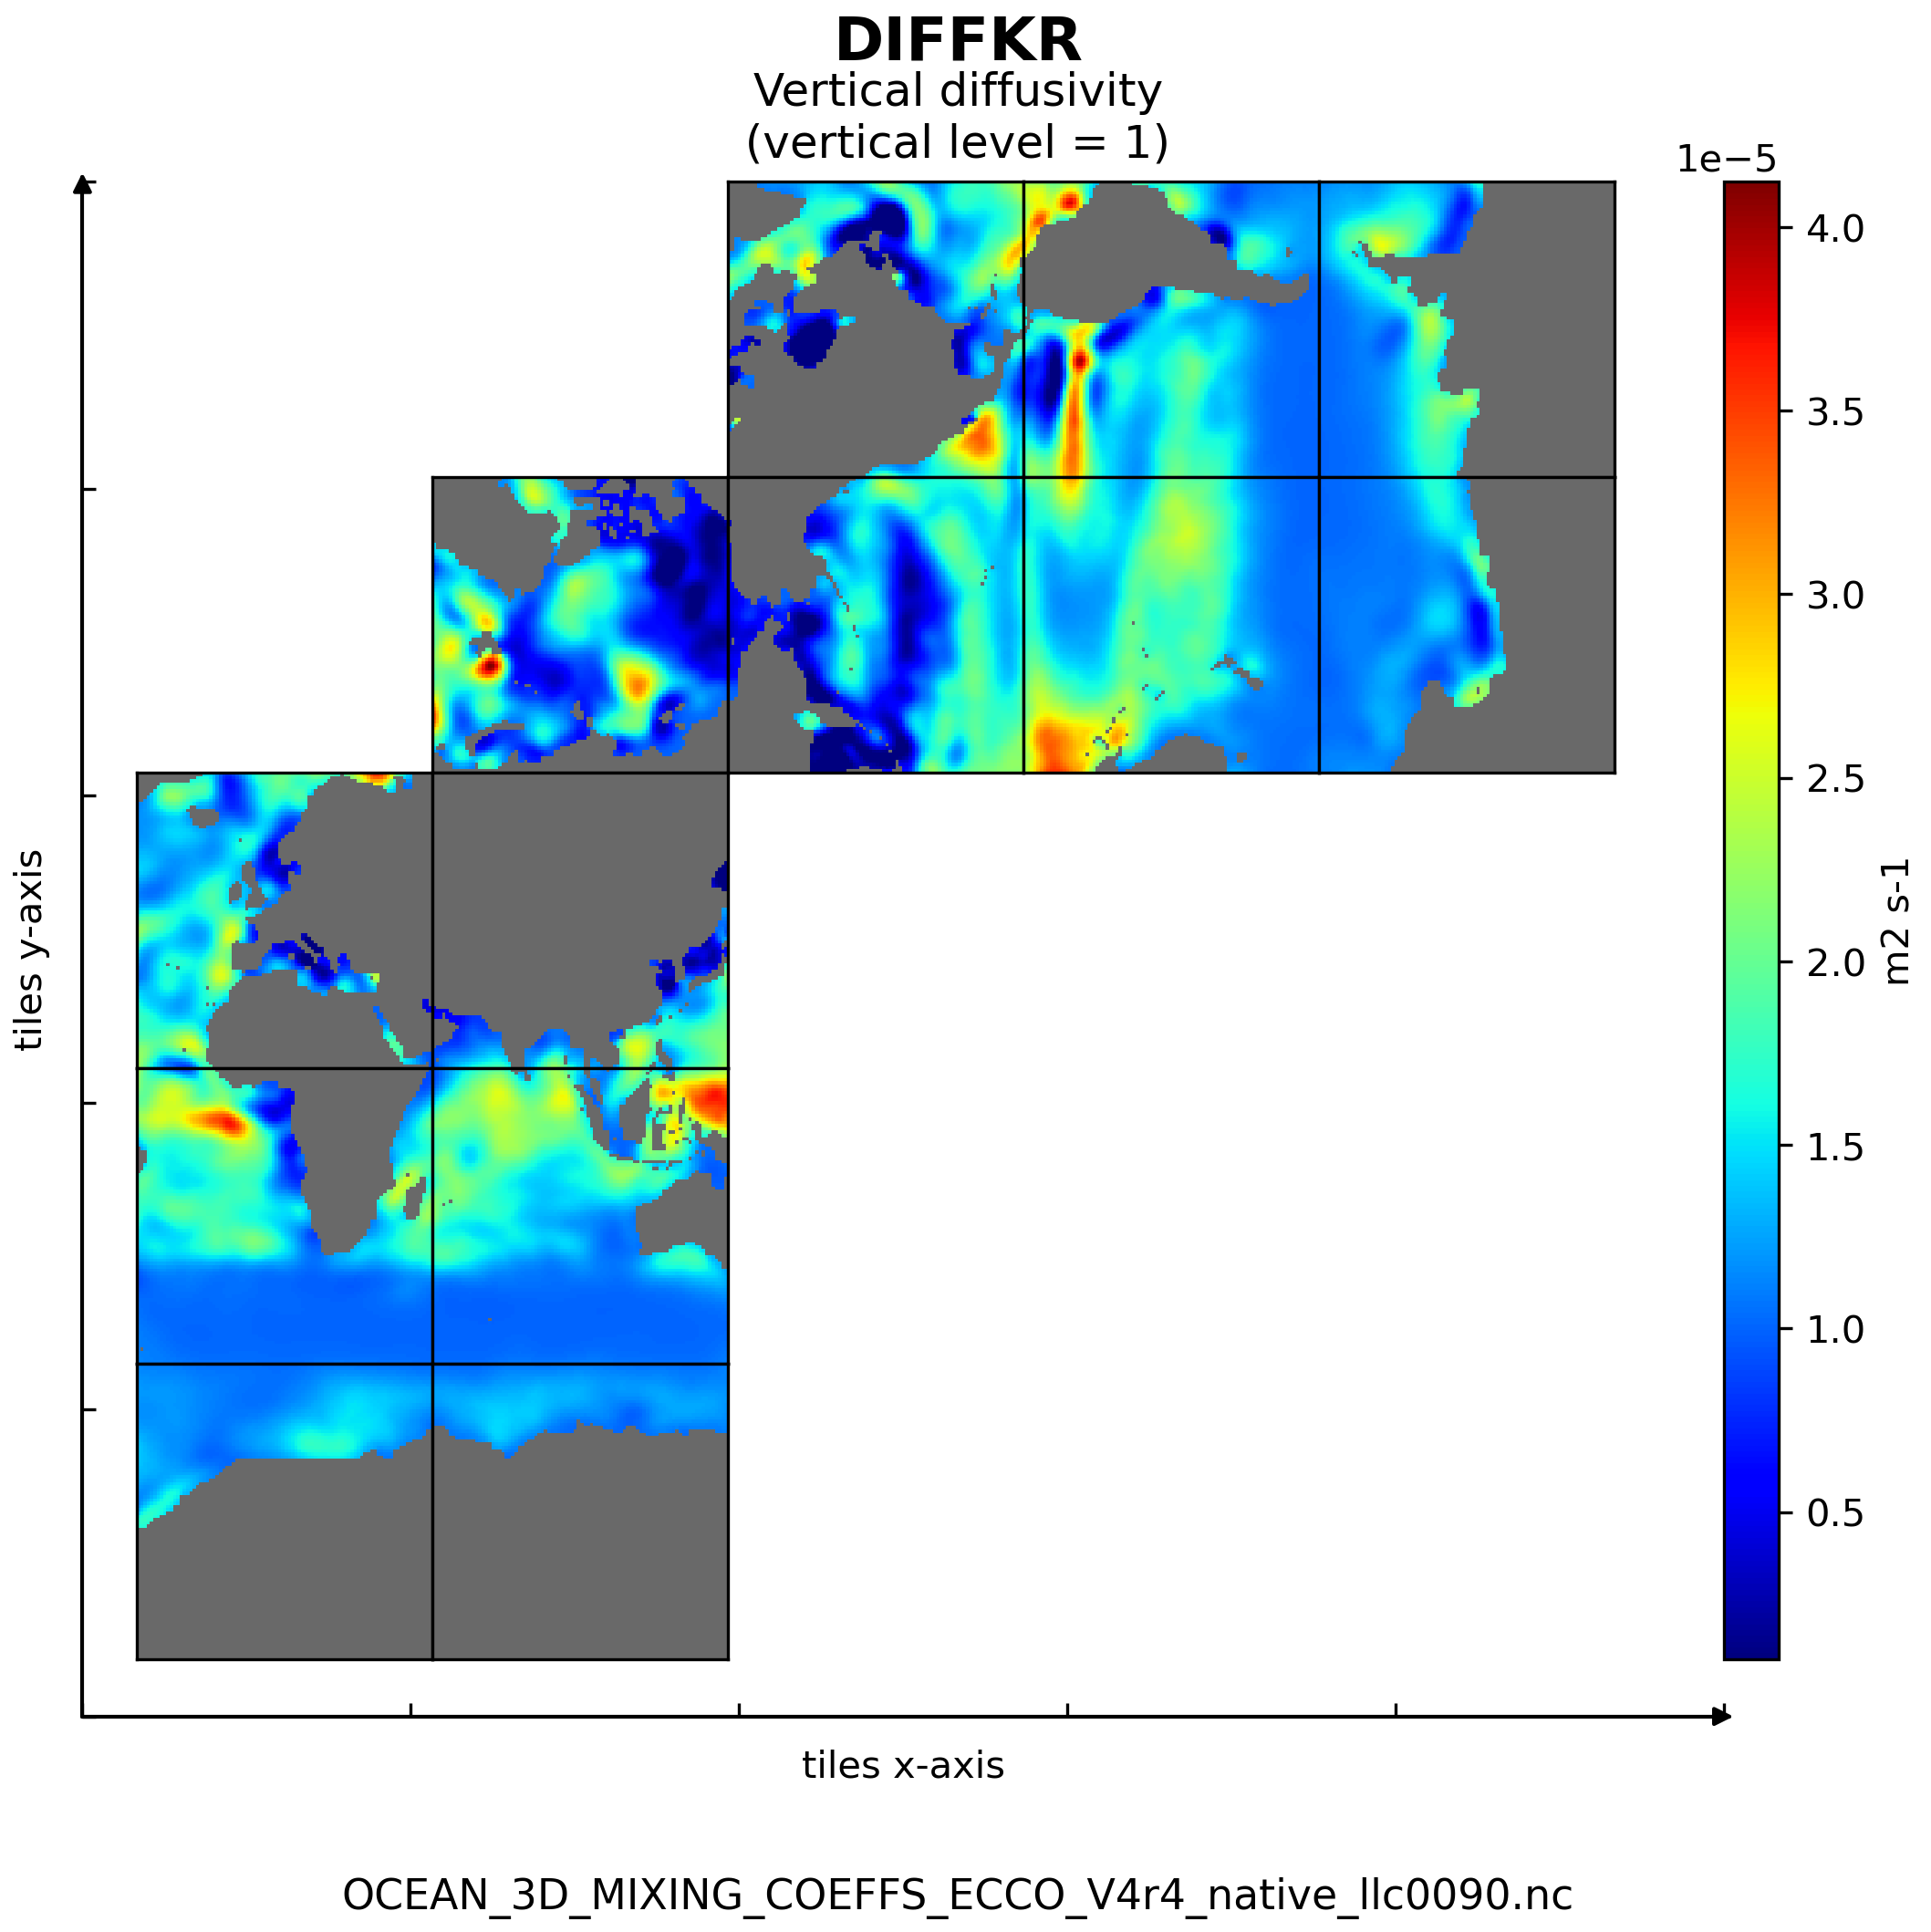
\includegraphics[scale=0.55]{../images/plots/v4r4/native_plots/Ocean_3D_Gent-Mcwilliams_Redi_and_Background_Vertical_Diffusivity_Coefficients_for_the_Lat-Lon-Cap_90_(llc90)_Native_Model_Grid_(Version_4_Release_4)/DIFFKR.png}
\caption{Dataset: OCEAN\_3D\_MIXING\_COEFFS, Variable: DIFFKR}
\label{tab:table-OCEAN_3D_MIXING_COEFFS_DIFFKR-Plot}
\end{figure}
\newpage
\pagebreak
\subsubsection{Native Variable: KAPGM}
\begin{longtable}{|m{0.06\textwidth}|m{0.3\textwidth}|m{0.45\textwidth}|m{0.12\textwidth}|}
\caption{Attributes description of the variable 'KAPGM' from OCEAN\_3D\_MIXING\_COEFFS's  dataset.}
\label{tab:table-OCEAN_3D_MIXING_COEFFS_KAPGM} \\ 
\hline \endhead \hline \endfoot
\rowcolor{lightgray} \textbf{Storage Type} & \textbf{Variable Name} & \textbf{Description} & \textbf{Unit} \\ \hline
float32 & KAPGM & Gent-mcwilliams diffusivity & m2 s-1 \\ \hline
\multicolumn{4}{|c|}{\cellcolor{lightgray}{\textbf{Description of the variable in Common Data language (CDL)}}} \\ \hline
\multicolumn{4}{|c|}{\fontfamily{lmtt}\selectfont{\makecell{\parbox{.95\textwidth}{\vspace*{0.25cm} \footnotesize{float32 KAPGM(k, tile, j, i)\\
\hspace*{0.5cm}KAPGM: \_FillValue = 9.96921e+36\\
\hspace*{0.5cm}KAPGM: coordinates = Z XC YC\\
\hspace*{0.5cm}KAPGM: coverage\_content\_type = modelResult\\
\hspace*{0.5cm}KAPGM: long\_name = Gent-McWilliams diffusivity\\
\hspace*{0.5cm}KAPGM: units = m2 s-1\\
\hspace*{0.5cm}KAPGM: valid\_max = 10000.0\\
\hspace*{0.5cm}KAPGM: valid\_min = 100.0\\
}}}}} \\ \hline
\rowcolor{lightgray} \multicolumn{4}{|c|}{\textbf{Comments}} \\ \hline
\multicolumn{4}{|p{1\textwidth}|}{\footnotesize{{Gent-mcwilliams diffusivity coefficient as described in gent and mcwilliams (1990, jpo). note: kapgm is a model control variable and has been optimized from a spatially invariant first guess of 1e3 m2 s-1.}}} \\ \hline
\end{longtable}

\begin{figure}[H]
\centering
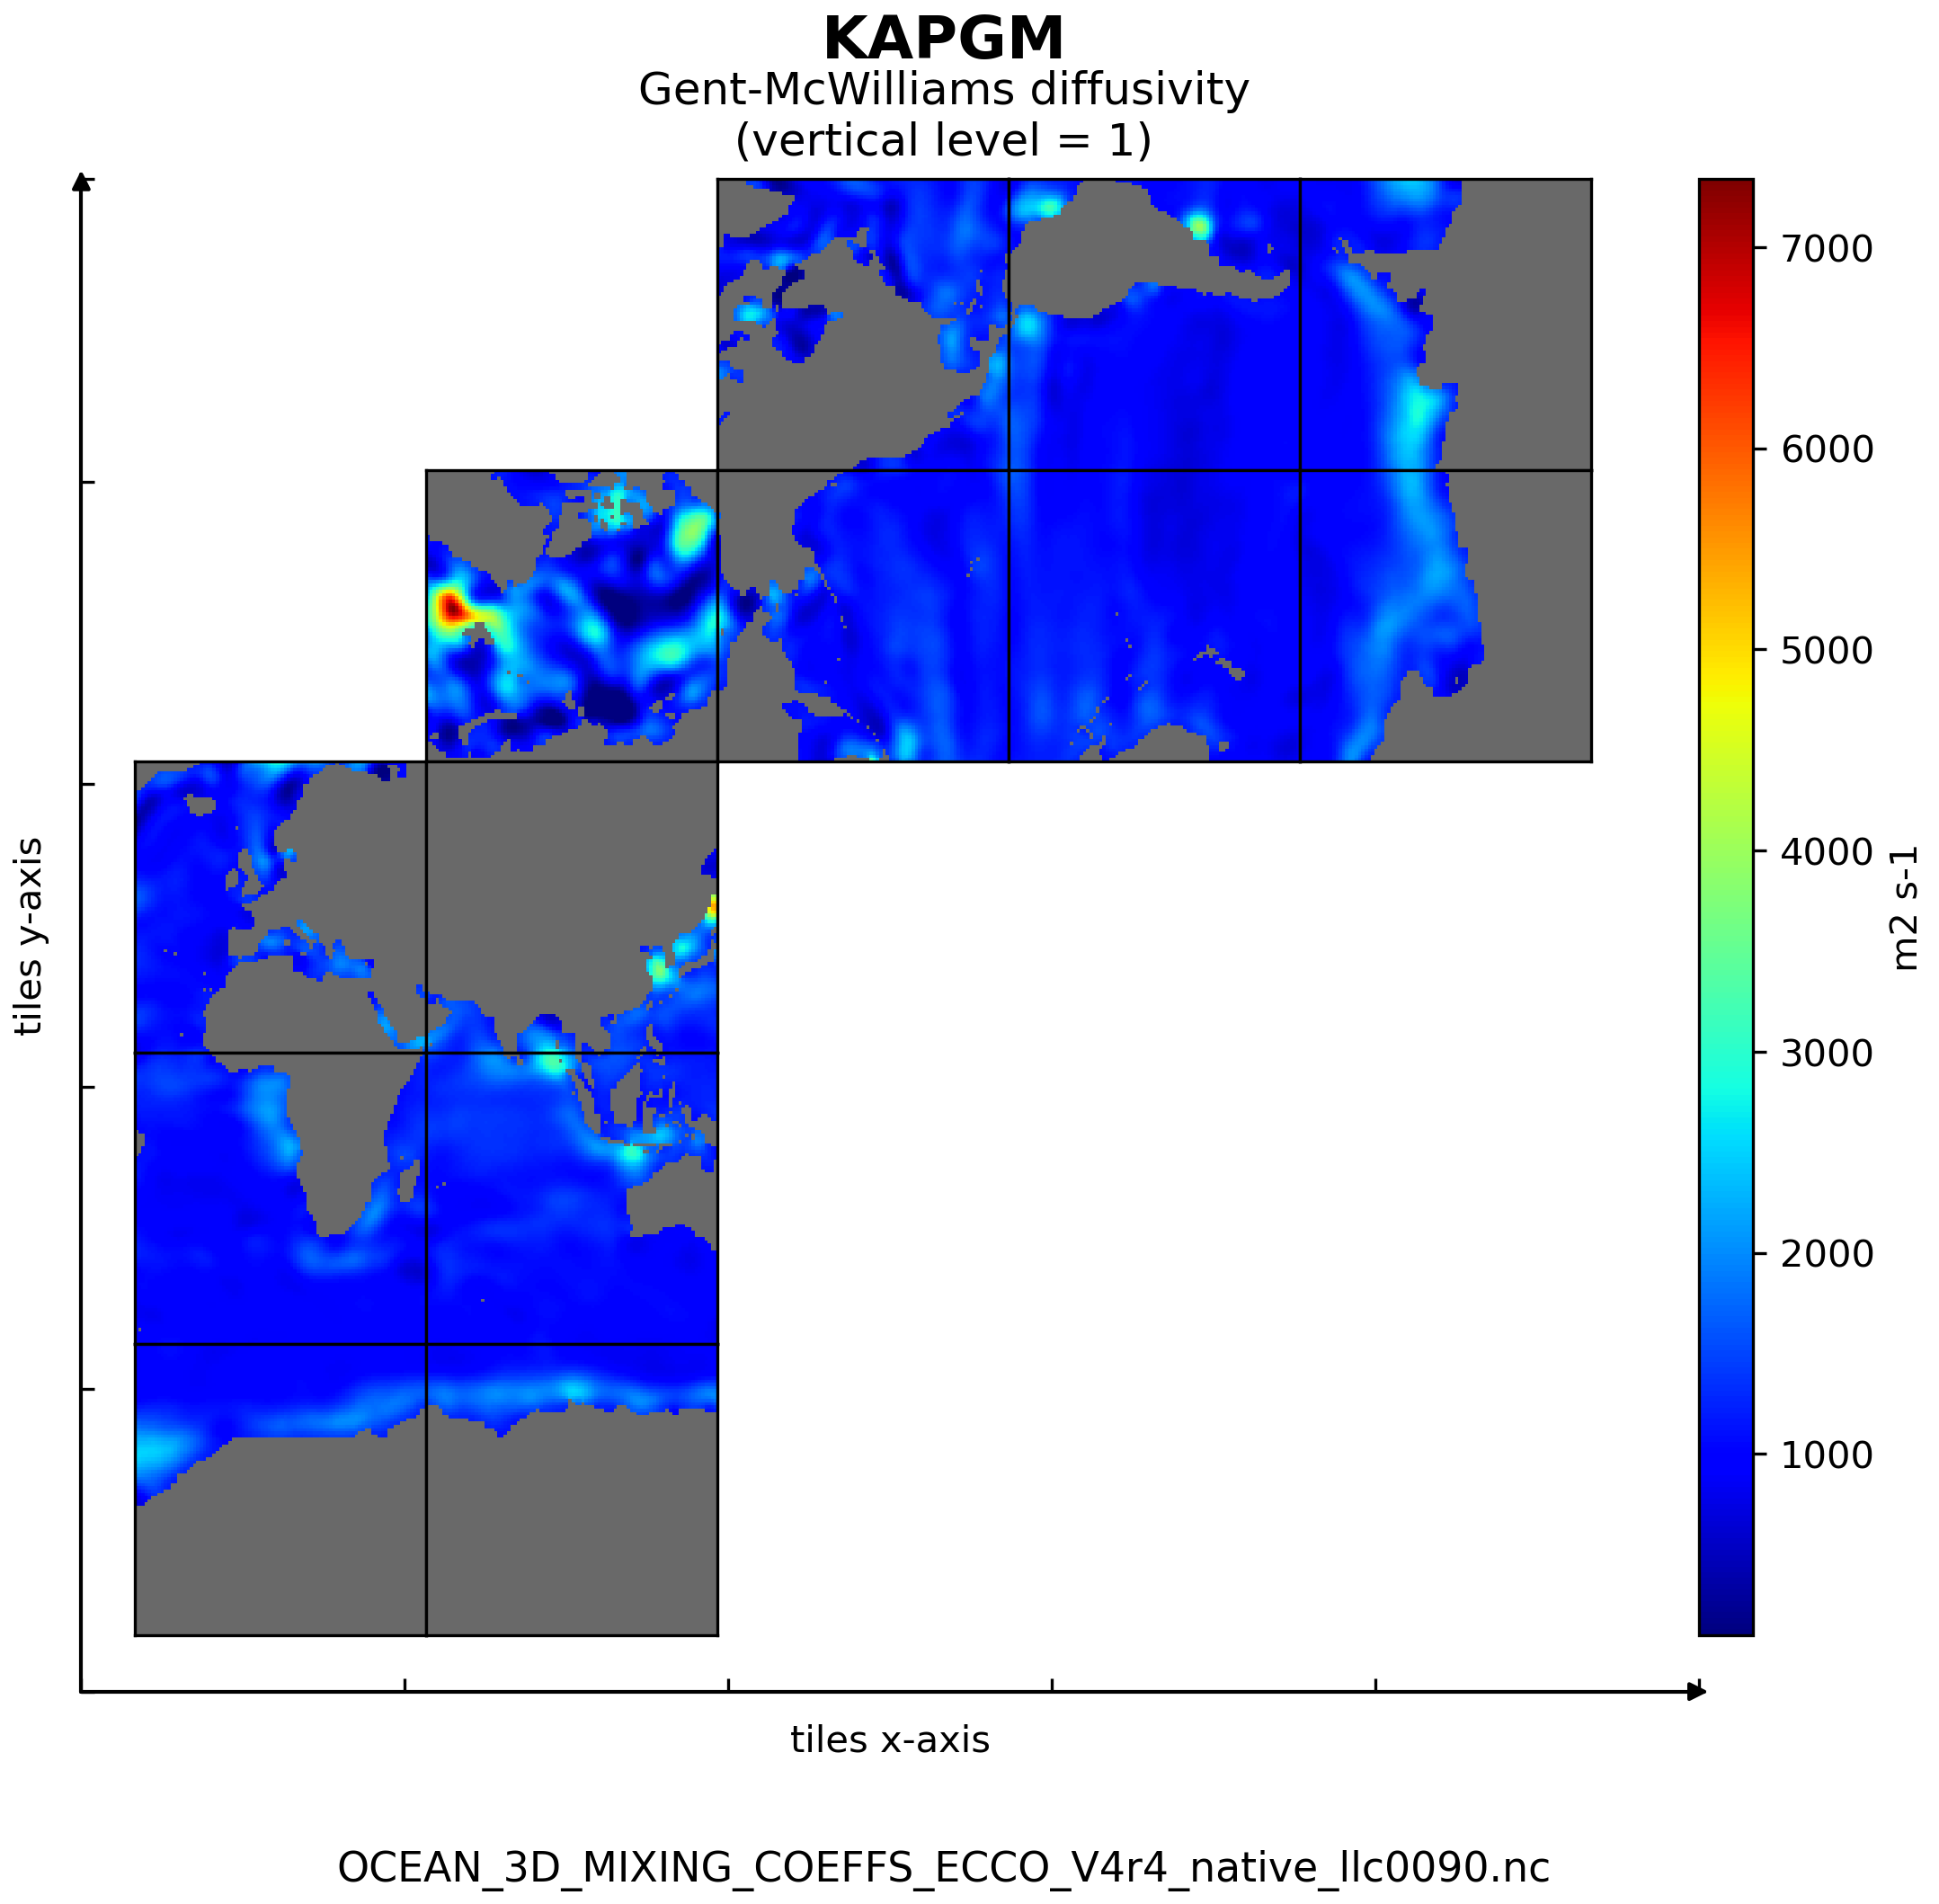
\includegraphics[scale=0.55]{../images/plots/v4r4/native_plots/Ocean_3D_Gent-Mcwilliams_Redi_and_Background_Vertical_Diffusivity_Coefficients_for_the_Lat-Lon-Cap_90_(llc90)_Native_Model_Grid_(Version_4_Release_4)/KAPGM.png}
\caption{Dataset: OCEAN\_3D\_MIXING\_COEFFS, Variable: KAPGM}
\label{tab:table-OCEAN_3D_MIXING_COEFFS_KAPGM-Plot}
\end{figure}
\newpage
\pagebreak
\subsubsection{Native Variable: KAPREDI}
\begin{longtable}{|m{0.06\textwidth}|m{0.3\textwidth}|m{0.45\textwidth}|m{0.12\textwidth}|}
\caption{Attributes description of the variable 'KAPREDI' from OCEAN\_3D\_MIXING\_COEFFS's  dataset.}
\label{tab:table-OCEAN_3D_MIXING_COEFFS_KAPREDI} \\ 
\hline \endhead \hline \endfoot
\rowcolor{lightgray} \textbf{Storage Type} & \textbf{Variable Name} & \textbf{Description} & \textbf{Unit} \\ \hline
float32 & KAPREDI & Along-isopycnal diffusivity & m2 s-1 \\ \hline
\multicolumn{4}{|c|}{\cellcolor{lightgray}{\textbf{Description of the variable in Common Data language (CDL)}}} \\ \hline
\multicolumn{4}{|c|}{\fontfamily{lmtt}\selectfont{\makecell{\parbox{.95\textwidth}{\vspace*{0.25cm} \footnotesize{float32 KAPREDI(k, tile, j, i)\\
\hspace*{0.5cm}KAPREDI: \_FillValue = 9.96921e+36\\
\hspace*{0.5cm}KAPREDI: coordinates = Z XC YC\\
\hspace*{0.5cm}KAPREDI: coverage\_content\_type = modelResult\\
\hspace*{0.5cm}KAPREDI: long\_name = Along-isopycnal diffusivity\\
\hspace*{0.5cm}KAPREDI: units = m2 s-1\\
\hspace*{0.5cm}KAPREDI: valid\_max = 10000.0\\
\hspace*{0.5cm}KAPREDI: valid\_min = 100.0\\
}}}}} \\ \hline
\rowcolor{lightgray} \multicolumn{4}{|c|}{\textbf{Comments}} \\ \hline
\multicolumn{4}{|p{1\textwidth}|}{\footnotesize{{Redi along-isopycnal diffusivity coefficient as described in redi (1982, jpo). note: kapredi is a model control variable and has been optimized from a spatially invariant first guess of 1e3 m2 s-1.}}} \\ \hline
\end{longtable}

\begin{figure}[H]
\centering
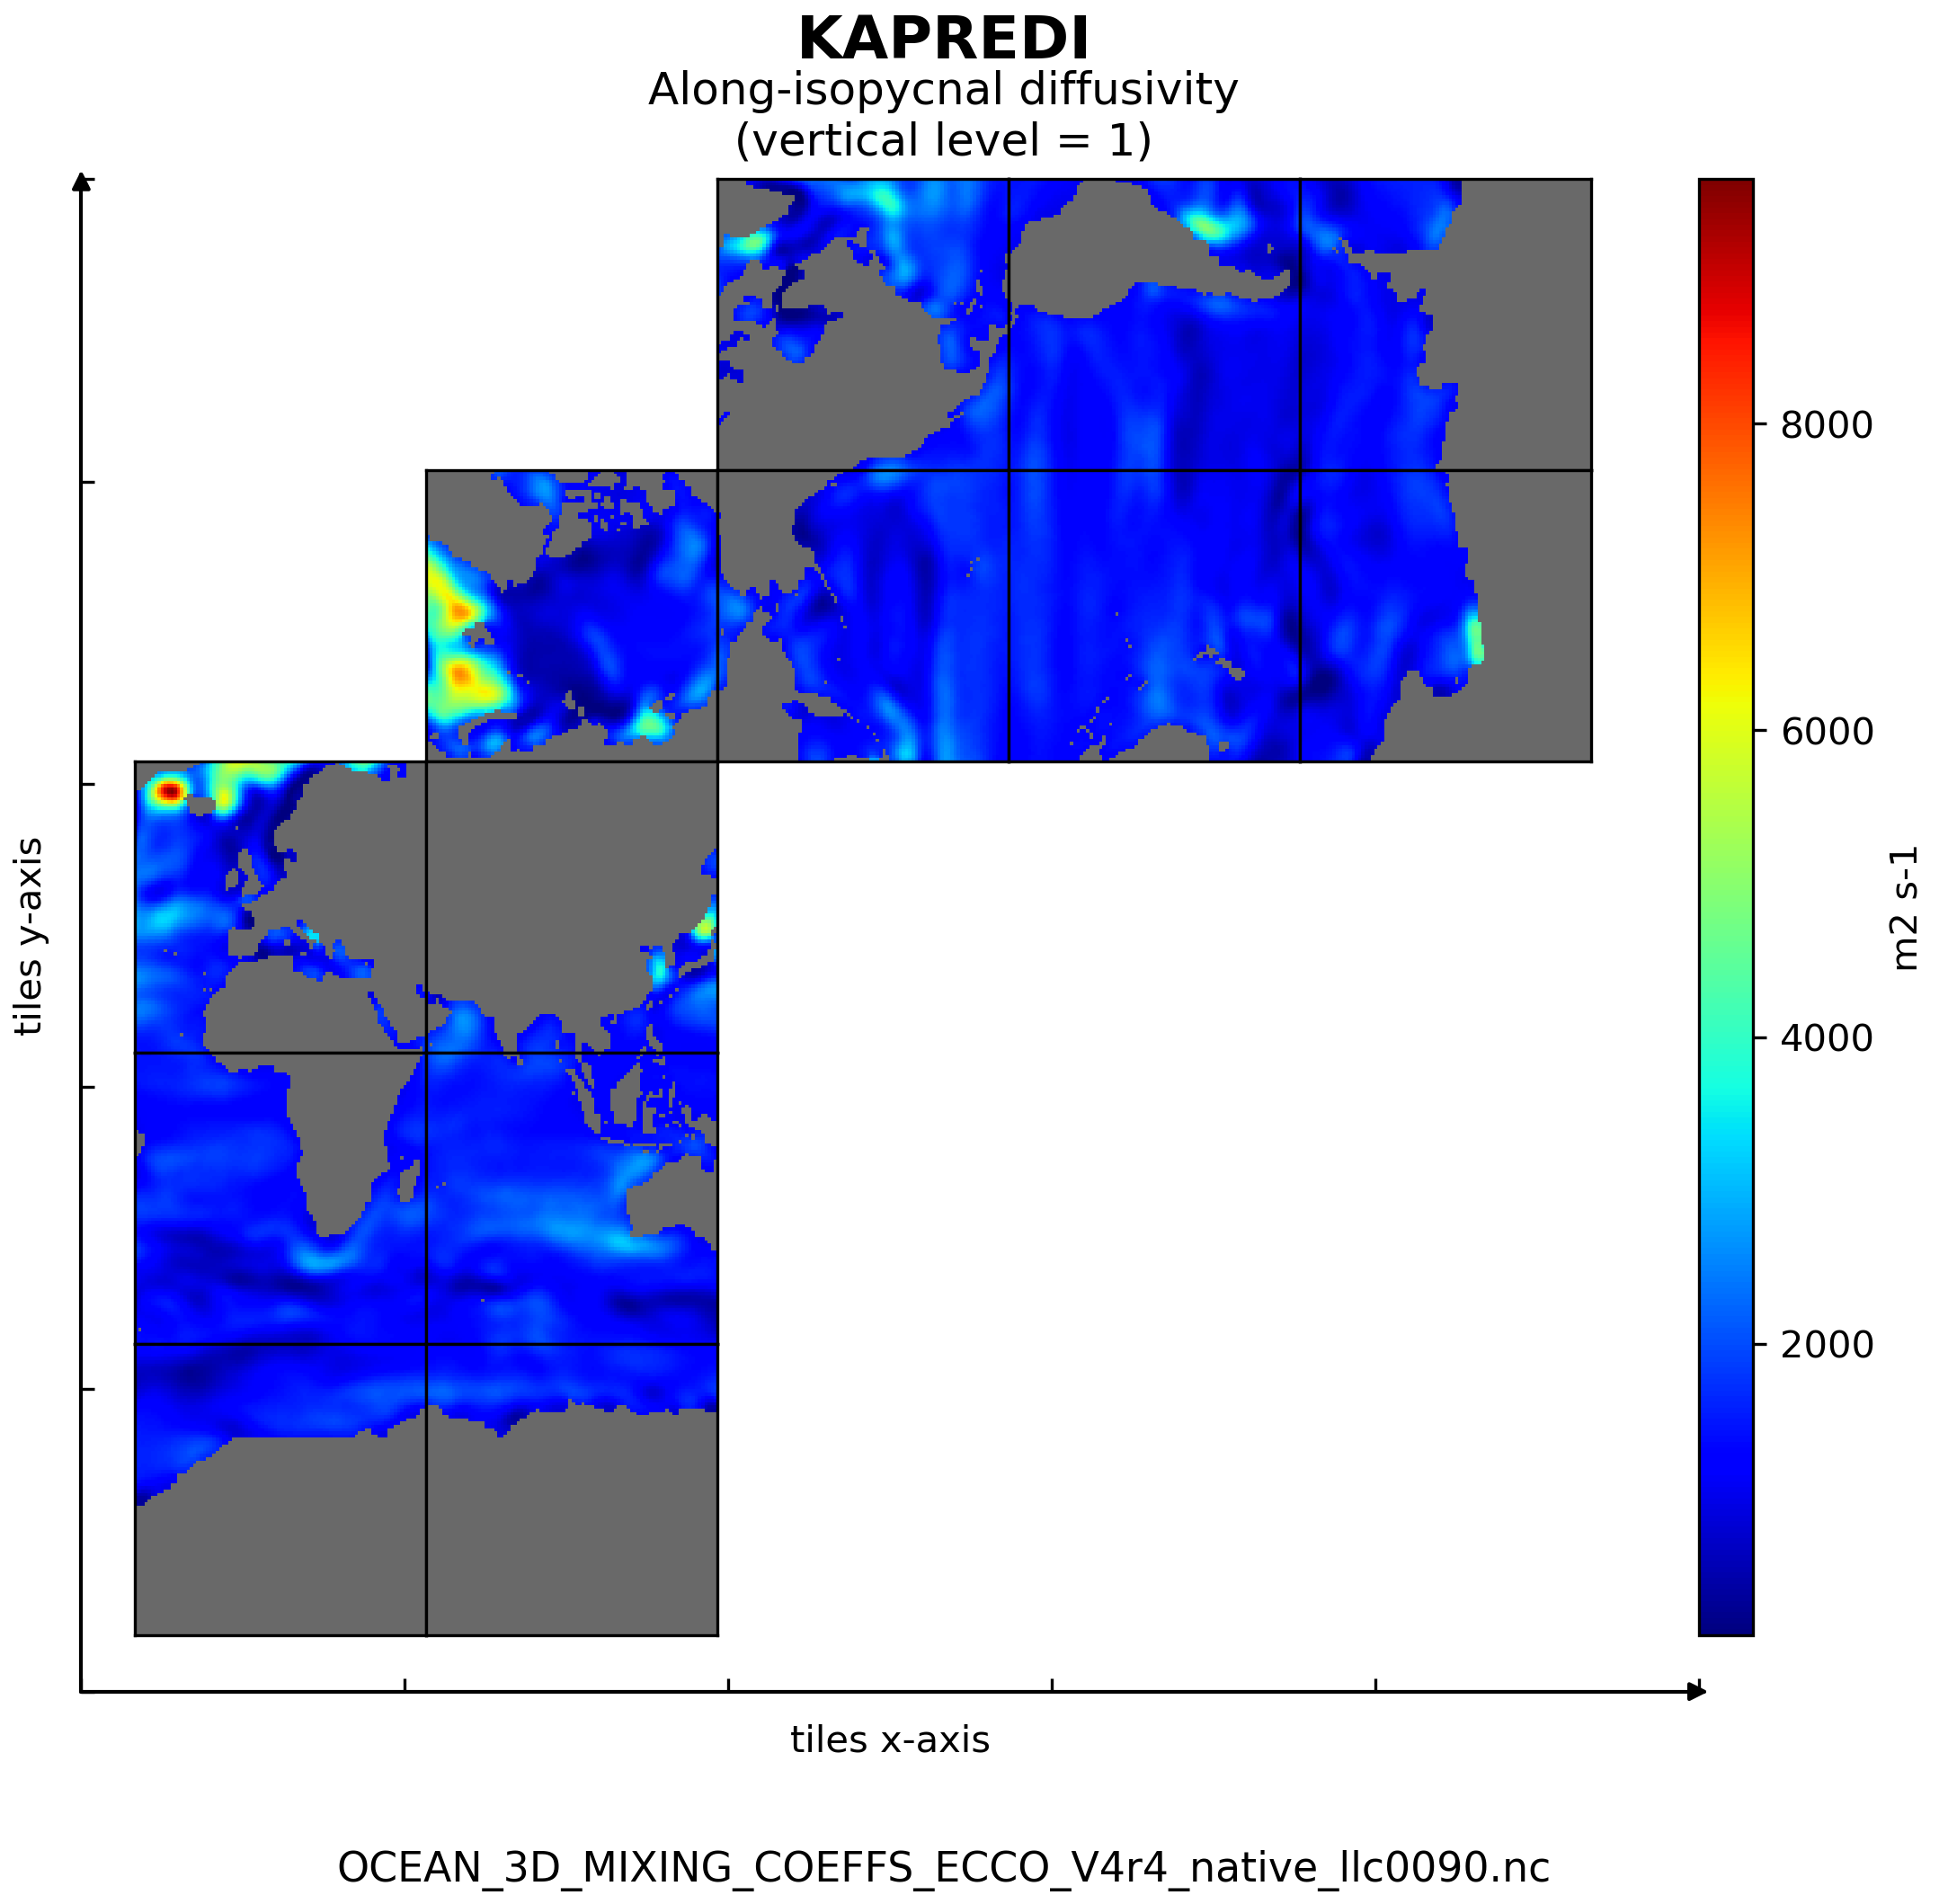
\includegraphics[scale=0.55]{../images/plots/v4r4/native_plots/Ocean_3D_Gent-Mcwilliams_Redi_and_Background_Vertical_Diffusivity_Coefficients_for_the_Lat-Lon-Cap_90_(llc90)_Native_Model_Grid_(Version_4_Release_4)/KAPREDI.png}
\caption{Dataset: OCEAN\_3D\_MIXING\_COEFFS, Variable: KAPREDI}
\label{tab:table-OCEAN_3D_MIXING_COEFFS_KAPREDI-Plot}
\end{figure}
\newpage
\subsection{Native dataset of OCEAN\_3D\_MOMENTUM\_TEND}
\newp
\subsubsection{Overview}
This dataset provides three-dimensional ocean momentum tendency on the lat-lon-cap 90 (llc90) native model grid from the ECCO Version 4 Release 4 (V4r4) ocean and sea-ice state estimate. The dataset is provided on daily-average and monthly-average time resolution. 
\begin{longtable}{|m{0.15\textwidth}|m{0.64\textwidth}|m{0.12\textwidth}|}
\caption{Coordinates and Variables in the dataset OCEAN\_3D\_MOMENTUM\_TEND}
\label{tab:table-OCEAN_3D_MOMENTUM_TEND-fields} \\ 
\hline \endhead \hline \endfoot
\rowcolor{lightgray} \multicolumn{1}{|c|}{\textbf{Coordinates}} & \multicolumn{1}{|c|}{\textbf{Description of data coordinates}} &  \multicolumn{1}{|c|}{\textbf{Unit}}\\ \hline
i &Grid index in x for variables at tracer and 'v' locations &--none--  \\ \hline
i\_g &Grid index in x for variables at 'u' and 'g' locations &--none--  \\ \hline
j &Grid index in y for variables at tracer and 'u' locations &--none--  \\ \hline
j\_g &Grid index in y for variables at 'v' and 'g' locations &--none--  \\ \hline
k &Grid index in z for tracer variables &--none--  \\ \hline
k\_u &Grid index in z corresponding to the bottom face of tracer grid cells ('w' locations) &--none--  \\ \hline
k\_l &Grid index in z corresponding to the top face of tracer grid cells ('w' locations) &--none--  \\ \hline
k\_p1 &Grid index in z for variables at 'w' locations &--none--  \\ \hline
tile &Lat-lon-cap tile index &--none--  \\ \hline
time &Center time of averaging period &--none--  \\ \hline
XC &Longitude of tracer grid cell center &degrees\_east  \\ \hline
YC &Latitude of tracer grid cell center &degrees\_north  \\ \hline
XG &Longitude of 'southwest' corner of tracer grid cell &degrees\_east  \\ \hline
YG &Latitude of 'southwest' corner of tracer grid cell &degrees\_north  \\ \hline
Z &Depth of tracer grid cell center &m  \\ \hline
Zp1 &Depth of tracer grid cell interface &m  \\ \hline
Zu &Depth of the bottom face of tracer grid cells &m  \\ \hline
Zl &Depth of the top face of tracer grid cells &m  \\ \hline
time\_bnds &Time bounds of averaging period &--none--  \\ \hline
XC\_bnds &Longitudes of tracer grid cell corners &--none--  \\ \hline
YC\_bnds &Latitudes of tracer grid cell corners &--none--  \\ \hline
Z\_bnds &Depths of tracer grid cell upper and lower interfaces &--none--  \\ \hline
\rowcolor{lightgray} \multicolumn{1}{|c|}{\textbf{Variables}} & \multicolumn{1}{|c|}{\textbf{Description of data variables}} &  \multicolumn{1}{|c|}{\textbf{Unit}}\\ \hline
Um\_dPHdx &Momentum tendency in the model +x direction &m s-2  \\ \hline
Vm\_dPHdy &Momentum tendency in the model +y direction &m s-2  \\ \hline
\end{longtable}

\newp
\pagebreak
\subsubsection{Native Variable: Um\_dPHdx}
\begin{longtable}{|m{0.06\textwidth}|m{0.3\textwidth}|m{0.45\textwidth}|m{0.12\textwidth}|}
\caption{Attributes description of the variable 'Um\_dPHdx' from OCEAN\_3D\_MOMENTUM\_TEND's  dataset.}
\label{tab:table-OCEAN_3D_MOMENTUM_TEND_Um_dPHdx} \\ 
\hline \endhead \hline \endfoot
\rowcolor{lightgray} \textbf{Storage Type} & \textbf{Variable Name} & \textbf{Description} & \textbf{Unit} \\ \hline
float32 & Um\_dPHdx & Momentum tendency in the model +x direction & m s-2 \\ \hline
\multicolumn{4}{|c|}{\cellcolor{lightgray}{\textbf{Description of the variable in Common Data language (CDL)}}} \\ \hline
\multicolumn{4}{|c|}{\fontfamily{lmtt}\selectfont{\makecell{\parbox{.95\textwidth}{\vspace*{0.25cm} \footnotesize{float32 Um\_dPHdx(time, k, tile, j, i\_g)\\
\hspace*{0.5cm}Um\_dPHdx: \_FillValue = 9.96921e+36\\
\hspace*{0.5cm}Um\_dPHdx: coordinates = time Z\\
\hspace*{0.5cm}Um\_dPHdx: coverage\_content\_type = modelResult\\
\hspace*{0.5cm}Um\_dPHdx: long\_name = Momentum tendency in the model +x direction\\
\hspace*{0.5cm}Um\_dPHdx: mate = Vm dPHdy\\
\hspace*{0.5cm}Um\_dPHdx: units = m s-2\\
\hspace*{0.5cm}Um\_dPHdx: valid\_max = 0.0011411579325795174\\
\hspace*{0.5cm}Um\_dPHdx: valid\_min = -0.0010651482734829187\\
}}}}} \\ \hline
\rowcolor{lightgray} \multicolumn{4}{|c|}{\textbf{Comments}} \\ \hline
\multicolumn{4}{|p{1\textwidth}|}{\footnotesize{{Momentum tendency in the +x direction due to the hydrostatic pressure gradient at the 'u' face of the native model grid cell . note: the model +x direction does not necessarily correspond to the geographical east-west direction because the x and y axes of the model's curvilinear lat-lon-cap (llc) grid have arbitrary orientations which vary within and across tiles.}}} \\ \hline
\end{longtable}

\begin{figure}[H]
\centering
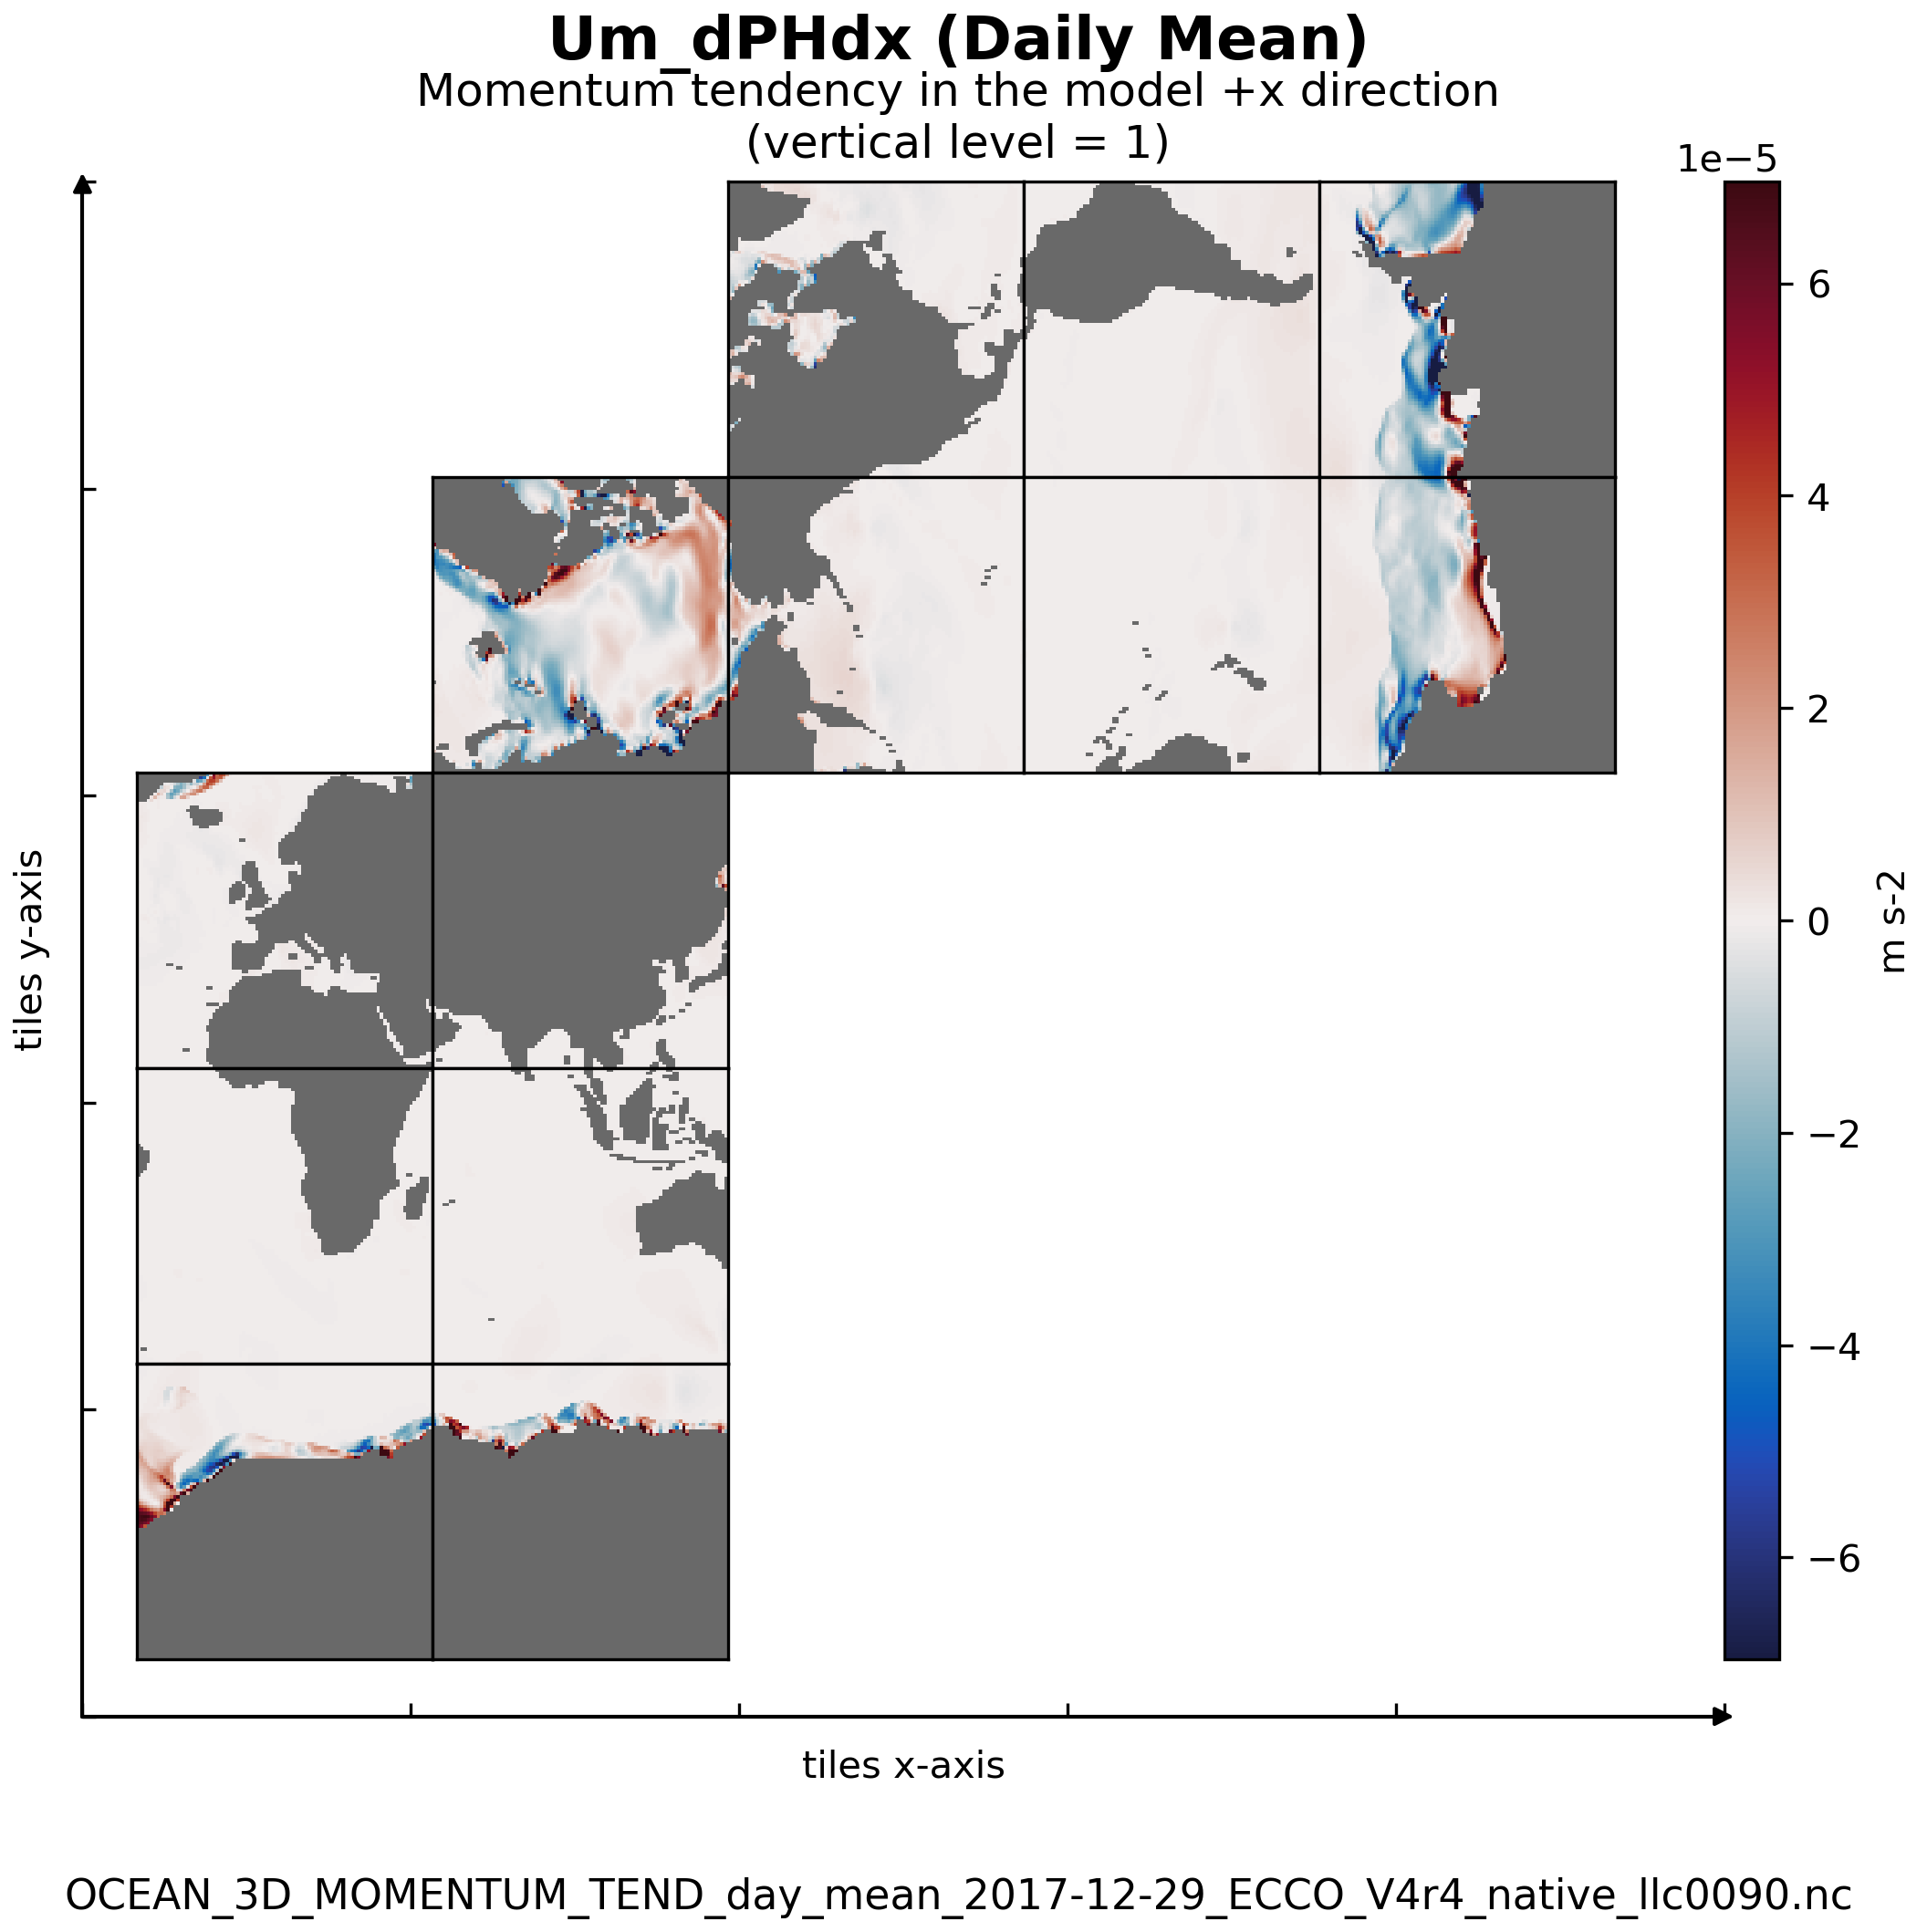
\includegraphics[scale=0.55]{../images/plots/v4r4/native_plots/Ocean_Three-Dimensional_Momentum_Tendency/Um_dPHdx.png}
\caption{Dataset: OCEAN\_3D\_MOMENTUM\_TEND, Variable: Um\_dPHdx}
\label{tab:table-OCEAN_3D_MOMENTUM_TEND_Um_dPHdx-Plot}
\end{figure}
\newpage
\pagebreak
\subsubsection{Native Variable: Vm\_dPHdy}
\begin{longtable}{|m{0.06\textwidth}|m{0.3\textwidth}|m{0.45\textwidth}|m{0.12\textwidth}|}
\caption{Attributes description of the variable 'Vm\_dPHdy' from OCEAN\_3D\_MOMENTUM\_TEND's  dataset.}
\label{tab:table-OCEAN_3D_MOMENTUM_TEND_Vm_dPHdy} \\ 
\hline \endhead \hline \endfoot
\rowcolor{lightgray} \textbf{Storage Type} & \textbf{Variable Name} & \textbf{Description} & \textbf{Unit} \\ \hline
float32 & Vm\_dPHdy & Momentum tendency in the model +y direction & m s-2 \\ \hline
\multicolumn{4}{|c|}{\cellcolor{lightgray}{\textbf{Description of the variable in Common Data language (CDL)}}} \\ \hline
\multicolumn{4}{|c|}{\fontfamily{lmtt}\selectfont{\makecell{\parbox{.95\textwidth}{\vspace*{0.25cm} \footnotesize{float32 Vm\_dPHdy(time, k, tile, j\_g, i)\\
\hspace*{0.5cm}Vm\_dPHdy: \_FillValue = 9.96921e+36\\
\hspace*{0.5cm}Vm\_dPHdy: coordinates = time Z\\
\hspace*{0.5cm}Vm\_dPHdy: coverage\_content\_type = modelResult\\
\hspace*{0.5cm}Vm\_dPHdy: long\_name = Momentum tendency in the model +y direction\\
\hspace*{0.5cm}Vm\_dPHdy: mate = Um dPHdx\\
\hspace*{0.5cm}Vm\_dPHdy: units = m s-2\\
\hspace*{0.5cm}Vm\_dPHdy: valid\_max = 0.0008858146029524505\\
\hspace*{0.5cm}Vm\_dPHdy: valid\_min = -0.0015932790702208877\\
}}}}} \\ \hline
\rowcolor{lightgray} \multicolumn{4}{|c|}{\textbf{Comments}} \\ \hline
\multicolumn{4}{|p{1\textwidth}|}{\footnotesize{{Momentum tendency in the +y direction due to the hydrostatic pressure gradient at the 'v' face of the native model grid cell . note: the model +y direction does not necessarily correspond to the geographical north-south direction because the x and y axes of the model's curvilinear lat-lon-cap (llc) grid have arbitrary orientations which vary within and across tiles.}}} \\ \hline
\end{longtable}

\begin{figure}[H]
\centering
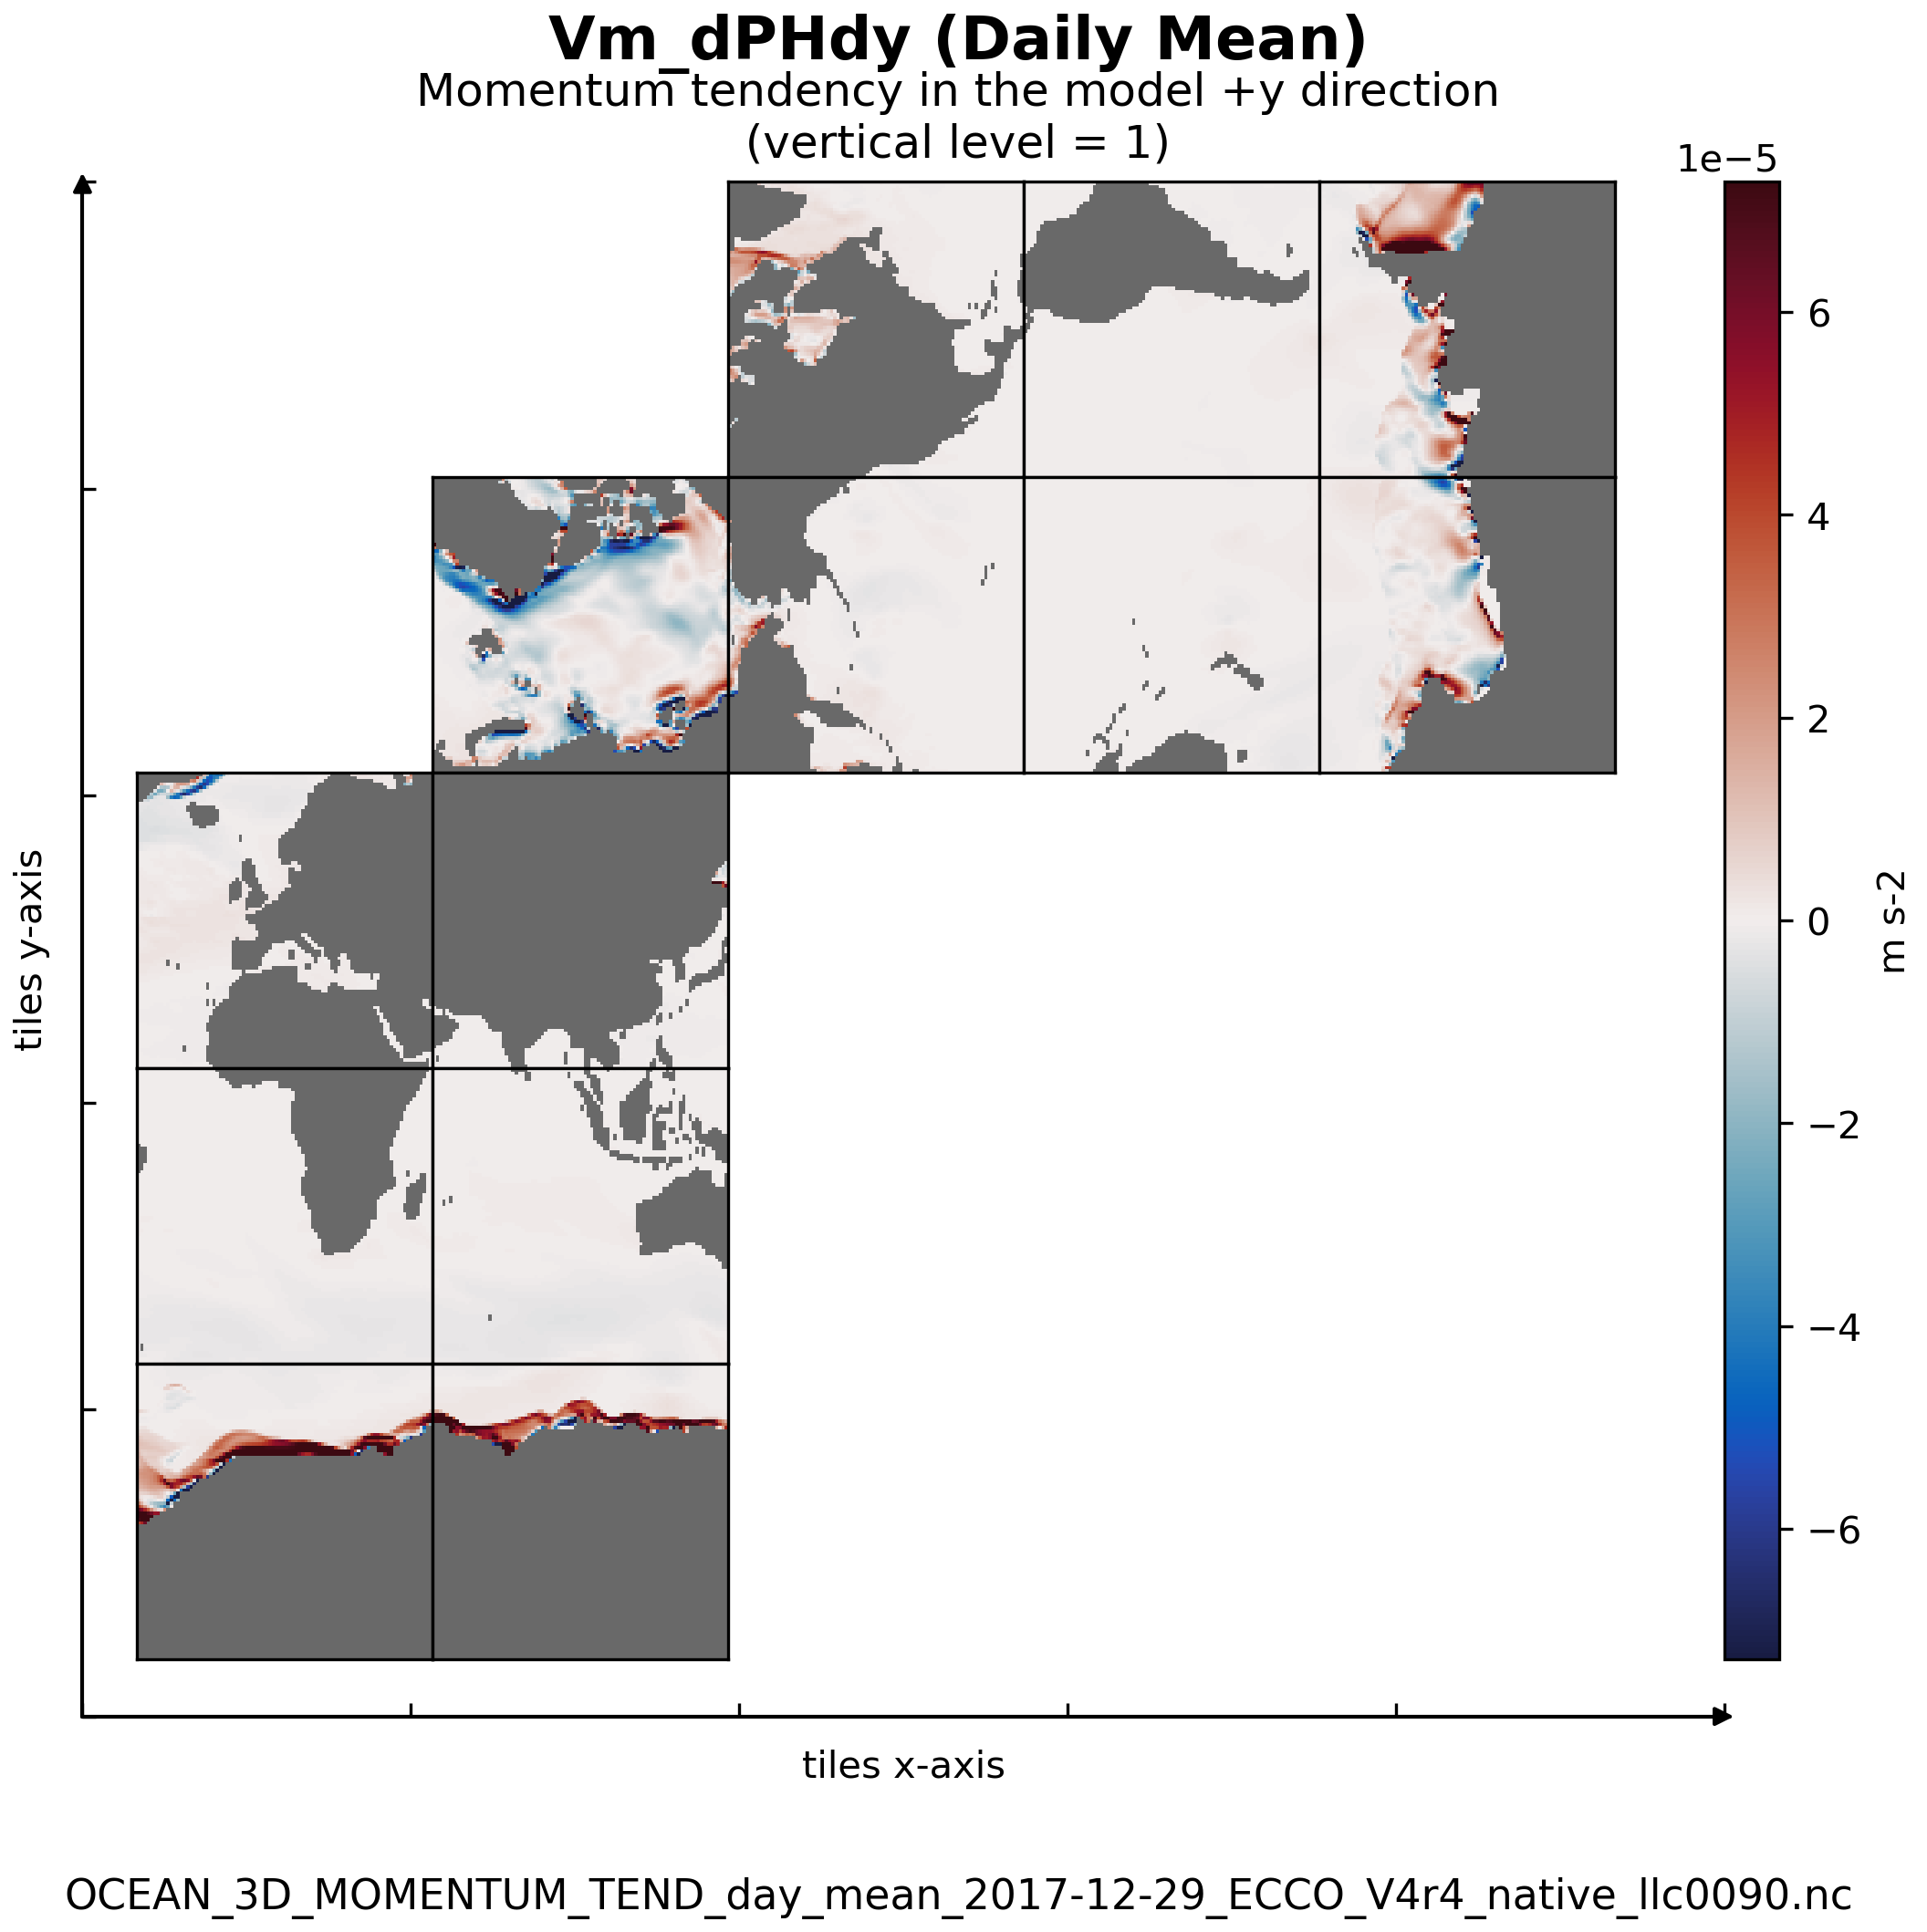
\includegraphics[scale=0.55]{../images/plots/v4r4/native_plots/Ocean_Three-Dimensional_Momentum_Tendency/Vm_dPHdy.png}
\caption{Dataset: OCEAN\_3D\_MOMENTUM\_TEND, Variable: Vm\_dPHdy}
\label{tab:table-OCEAN_3D_MOMENTUM_TEND_Vm_dPHdy-Plot}
\end{figure}
\newpage
\subsection{Native dataset of OCEAN\_3D\_SALINITY\_FLUX}
\newp
\subsubsection{Overview}
This dataset provides three-dimensional ocean salinity fluxes on the lat-lon-cap 90 (llc90) native model grid from the ECCO Version 4 Release 4 (V4r4) ocean and sea-ice state estimate. The dataset is provided on daily-average and monthly-average time resolution. ADV*\_SLT and DF*\_SLT terms are salinity fluxes. oceSPtnd is salt tendency per unit area (g m-2 s-1), not salinity flux. 
\begin{longtable}{|m{0.15\textwidth}|m{0.64\textwidth}|m{0.12\textwidth}|}
\caption{Coordinates and Variables in the dataset OCEAN\_3D\_SALINITY\_FLUX}
\label{tab:table-OCEAN_3D_SALINITY_FLUX-fields} \\ 
\hline \endhead \hline \endfoot
\rowcolor{lightgray} \multicolumn{1}{|c|}{\textbf{Coordinates}} & \multicolumn{1}{|c|}{\textbf{Description of data coordinates}} &  \multicolumn{1}{|c|}{\textbf{Unit}}\\ \hline
i &Grid index in x for variables at tracer and 'v' locations &--none--  \\ \hline
i\_g &Grid index in x for variables at 'u' and 'g' locations &--none--  \\ \hline
j &Grid index in y for variables at tracer and 'u' locations &--none--  \\ \hline
j\_g &Grid index in y for variables at 'v' and 'g' locations &--none--  \\ \hline
k &Grid index in z for tracer variables &--none--  \\ \hline
k\_u &Grid index in z corresponding to the bottom face of tracer grid cells ('w' locations) &--none--  \\ \hline
k\_l &Grid index in z corresponding to the top face of tracer grid cells ('w' locations) &--none--  \\ \hline
k\_p1 &Grid index in z for variables at 'w' locations &--none--  \\ \hline
tile &Lat-lon-cap tile index &--none--  \\ \hline
time &Center time of averaging period &--none--  \\ \hline
XC &Longitude of tracer grid cell center &degrees\_east  \\ \hline
YC &Latitude of tracer grid cell center &degrees\_north  \\ \hline
XG &Longitude of 'southwest' corner of tracer grid cell &degrees\_east  \\ \hline
YG &Latitude of 'southwest' corner of tracer grid cell &degrees\_north  \\ \hline
Z &Depth of tracer grid cell center &m  \\ \hline
Zp1 &Depth of tracer grid cell interface &m  \\ \hline
Zu &Depth of the bottom face of tracer grid cells &m  \\ \hline
Zl &Depth of the top face of tracer grid cells &m  \\ \hline
time\_bnds &Time bounds of averaging period &--none--  \\ \hline
XC\_bnds &Longitudes of tracer grid cell corners &--none--  \\ \hline
YC\_bnds &Latitudes of tracer grid cell corners &--none--  \\ \hline
Z\_bnds &Depths of tracer grid cell upper and lower interfaces &--none--  \\ \hline
\rowcolor{lightgray} \multicolumn{1}{|c|}{\textbf{Variables}} & \multicolumn{1}{|c|}{\textbf{Description of data variables}} &  \multicolumn{1}{|c|}{\textbf{Unit}}\\ \hline
ADVx\_SLT &Lateral advective flux of salinity in the model +x direction &1e-3 m3 s-1  \\ \hline
DFxE\_SLT &Lateral diffusive flux of salinity in the model +x direction &1e-3 m3 s-1  \\ \hline
ADVy\_SLT &Lateral advective flux of salinity in the model +y direction &1e-3 m3 s-1  \\ \hline
DFyE\_SLT &Lateral diffusive flux of salinity in the model +y direction &1e-3 m3 s-1  \\ \hline
ADVr\_SLT &Vertical advective flux of salinity &1e-3 m3 s-1  \\ \hline
DFrE\_SLT &Vertical diffusive flux of salinity (explicit term) &1e-3 m3 s-1  \\ \hline
DFrI\_SLT &Vertical diffusive flux of salinity (implicit term) &1e-3 m3 s-1  \\ \hline
oceSPtnd &Salt tendency due to the vertical transport of salt in high-salinity brine plumes &g m-2 s-1  \\ \hline
\end{longtable}

\newp
\pagebreak
\subsubsection{Native Variable: ADVr\_SLT}
\begin{longtable}{|m{0.06\textwidth}|m{0.3\textwidth}|m{0.45\textwidth}|m{0.12\textwidth}|}
\caption{Attributes description of the variable 'ADVr\_SLT' from OCEAN\_3D\_SALINITY\_FLUX's  dataset.}
\label{tab:table-OCEAN_3D_SALINITY_FLUX_ADVr_SLT} \\ 
\hline \endhead \hline \endfoot
\rowcolor{lightgray} \textbf{Storage Type} & \textbf{Variable Name} & \textbf{Description} & \textbf{Unit} \\ \hline
float32 & ADVr\_SLT & Vertical advective flux of salinity & 1e-3 m3 s-1 \\ \hline
\multicolumn{4}{|c|}{\cellcolor{lightgray}{\textbf{Description of the variable in Common Data language (CDL)}}} \\ \hline
\multicolumn{4}{|c|}{\fontfamily{lmtt}\selectfont{\makecell{\parbox{.95\textwidth}{\vspace*{0.25cm} \footnotesize{float32 ADVr\_SLT(time, k\_l, tile, j, i)\\
\hspace*{0.5cm}ADVr\_SLT: \_FillValue = 9.96921e+36\\
\hspace*{0.5cm}ADVr\_SLT: coordinates = XC Zl YC time\\
\hspace*{0.5cm}ADVr\_SLT: coverage\_content\_type = modelResult\\
\hspace*{0.5cm}ADVr\_SLT: direction = >0 decreases salinity (SALT)\\
\hspace*{0.5cm}ADVr\_SLT: long\_name = Vertical advective flux of salinity\\
\hspace*{0.5cm}ADVr\_SLT: units = 1e-3 m3 s-1\\
\hspace*{0.5cm}ADVr\_SLT: valid\_max = 263294624.0\\
\hspace*{0.5cm}ADVr\_SLT: valid\_min = -324149856.0\\
}}}}} \\ \hline
\rowcolor{lightgray} \multicolumn{4}{|c|}{\textbf{Comments}} \\ \hline
\multicolumn{4}{|p{1\textwidth}|}{\footnotesize{{Vertical advective flux of salinity (salt) in the +z direction through the top 'w' face of the tracer cell on the native model grid. note: in the arakawa-c grid, vertical flux quantities are staggered relative to the tracer cells with indexing such that +advr\_slt(i,j,k\_l) corresponds to upward +z fluxes through the top 'w' face of the tracer cell at (i,j,k). salinity defined using cf convention 'sea water salinity is the salt content of sea water, often on the practical salinity scale of 1978. however, the unqualified term 'salinity' is generic and does not necessarily imply any particular method of calculation. the units of salinity are dimensionless and the units attribute should normally be given as 1e-3 or 0.001 i.e. parts per thousand.' see https://cfconventions.org/data/cf-standard-names/73/build/cf-standard-name-table.html}}} \\ \hline
\end{longtable}

\begin{figure}[H]
\centering
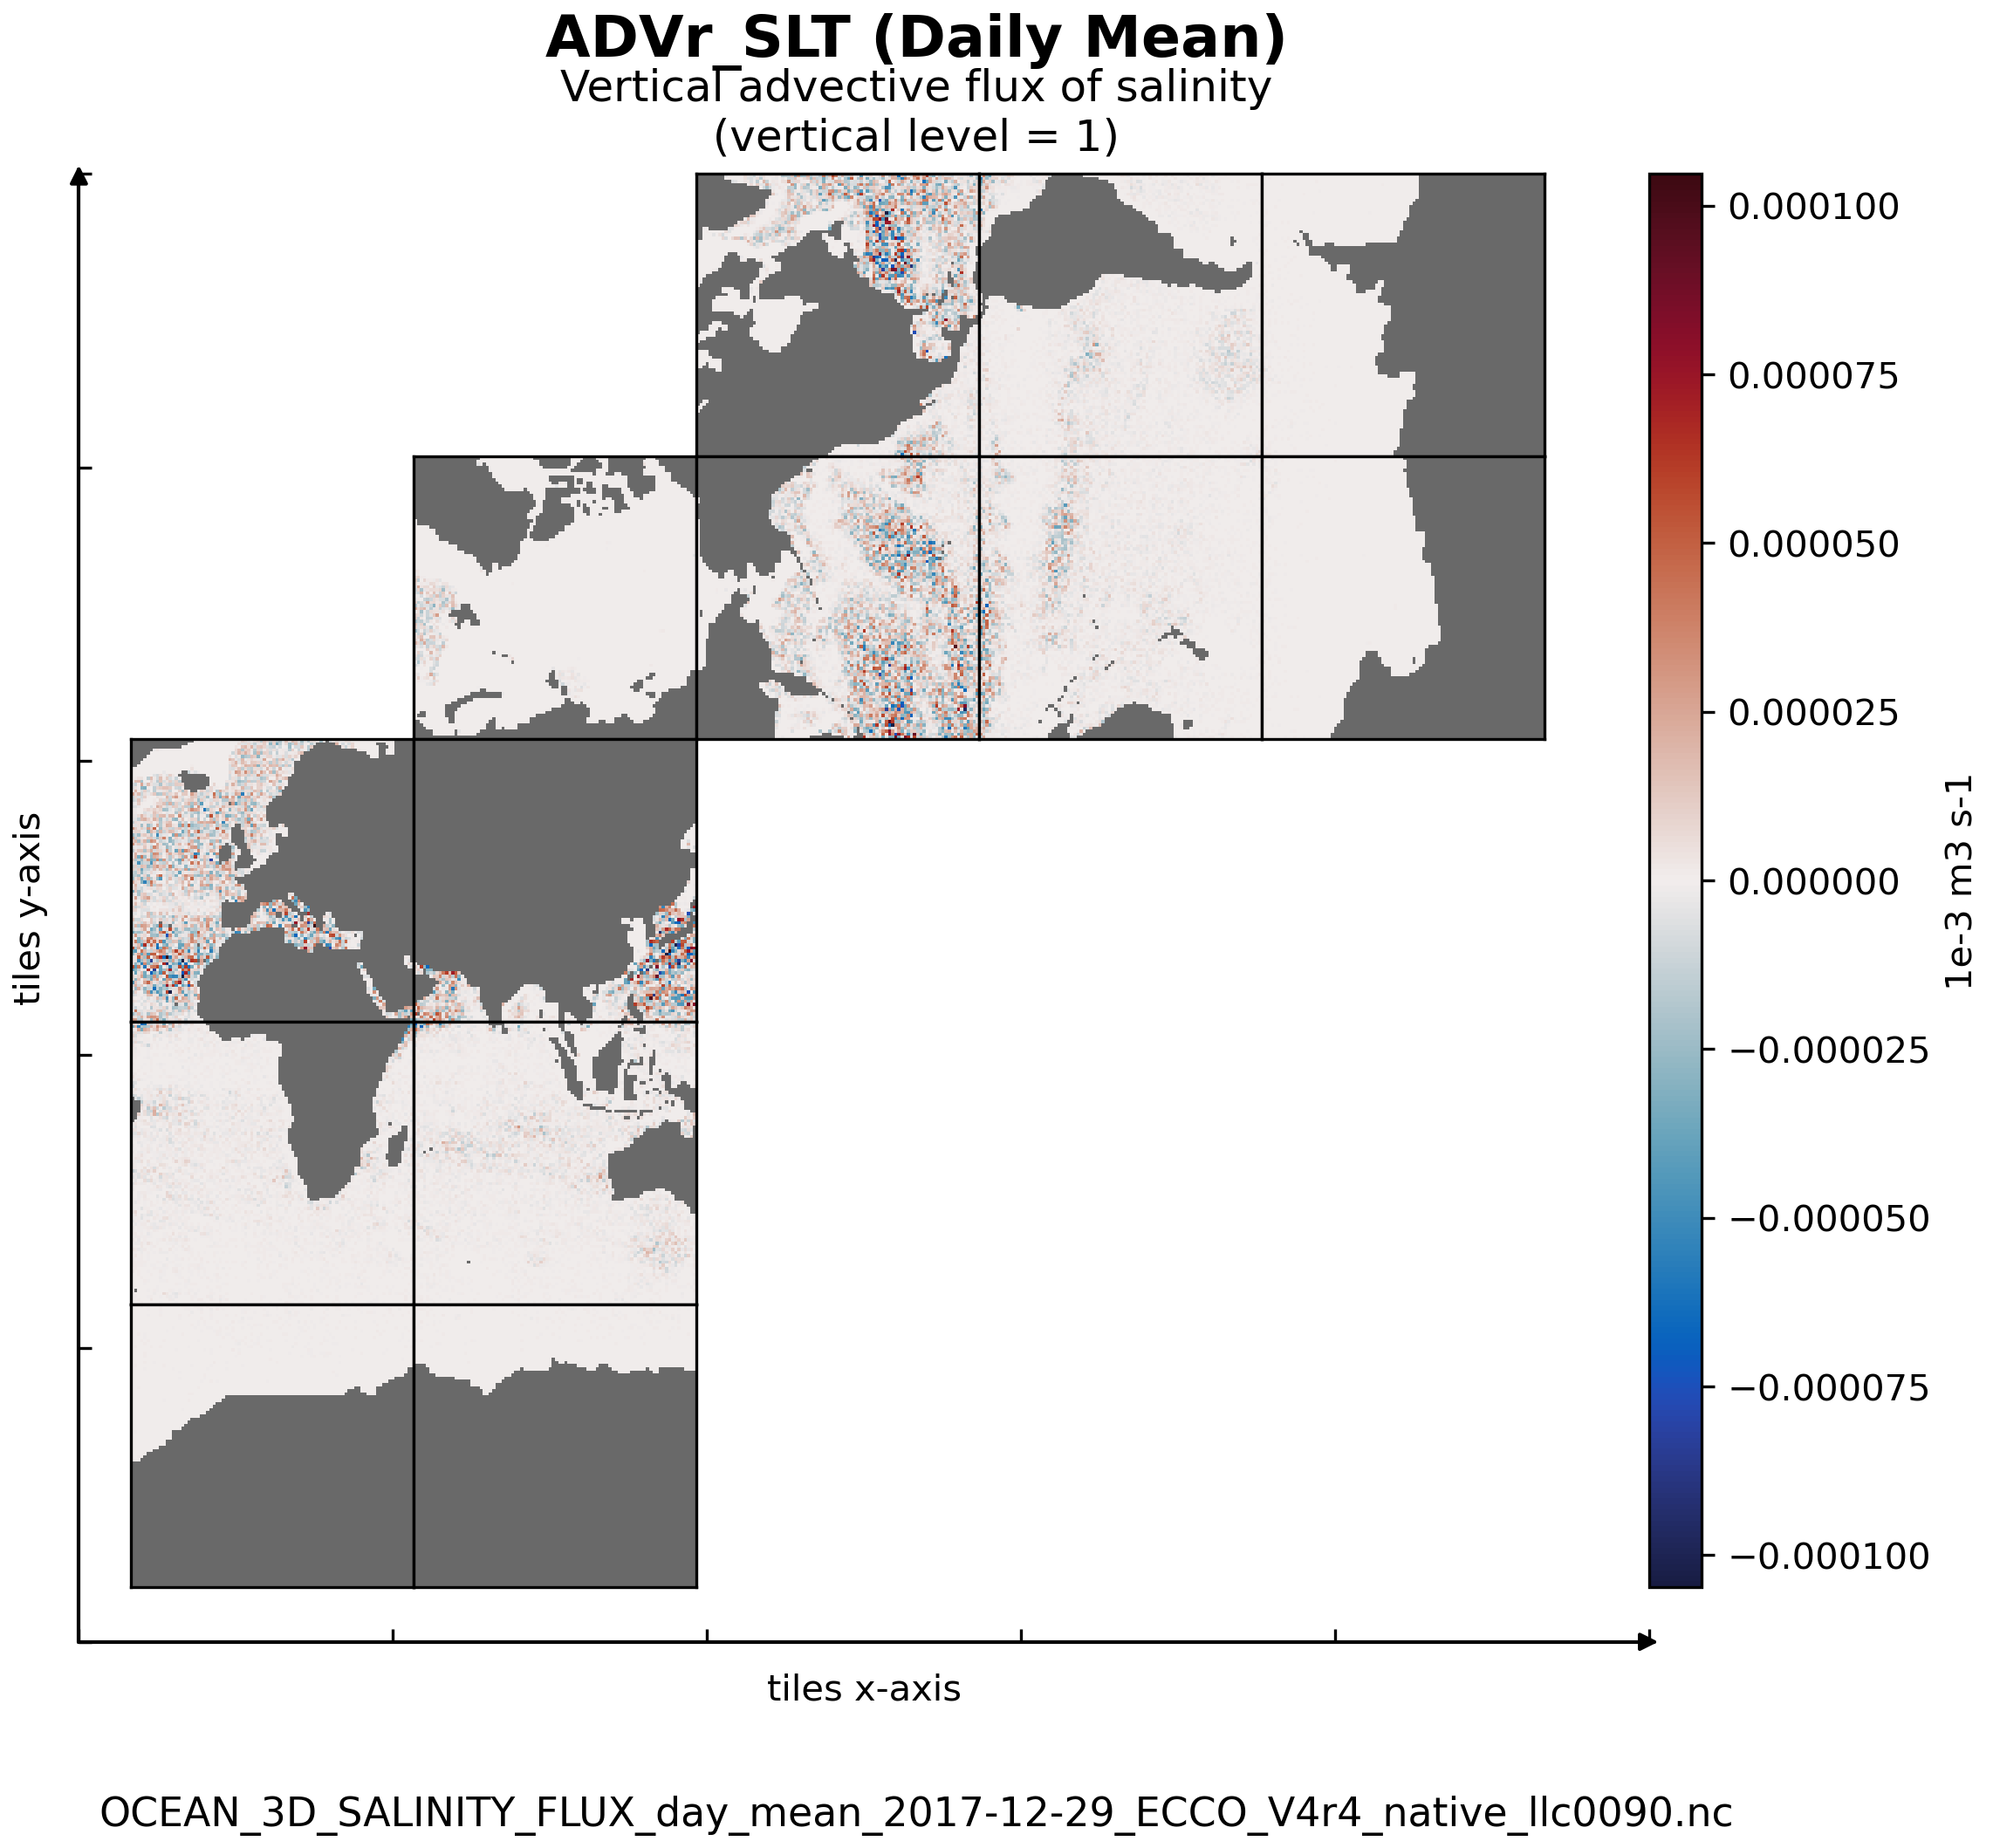
\includegraphics[scale=0.55]{../images/plots/v4r4/native_plots/Ocean_Three-Dimensional_Salinity_Fluxes/ADVr_SLT.png}
\caption{Dataset: OCEAN\_3D\_SALINITY\_FLUX, Variable: ADVr\_SLT}
\label{tab:table-OCEAN_3D_SALINITY_FLUX_ADVr_SLT-Plot}
\end{figure}
\newpage
\pagebreak
\subsubsection{Native Variable: ADVx\_SLT}
\begin{longtable}{|m{0.06\textwidth}|m{0.3\textwidth}|m{0.45\textwidth}|m{0.12\textwidth}|}
\caption{Attributes description of the variable 'ADVx\_SLT' from OCEAN\_3D\_SALINITY\_FLUX's  dataset.}
\label{tab:table-OCEAN_3D_SALINITY_FLUX_ADVx_SLT} \\ 
\hline \endhead \hline \endfoot
\rowcolor{lightgray} \textbf{Storage Type} & \textbf{Variable Name} & \textbf{Description} & \textbf{Unit} \\ \hline
float32 & ADVx\_SLT & Lateral advective flux of salinity in the model +x direction & 1e-3 m3 s-1 \\ \hline
\multicolumn{4}{|c|}{\cellcolor{lightgray}{\textbf{Description of the variable in Common Data language (CDL)}}} \\ \hline
\multicolumn{4}{|c|}{\fontfamily{lmtt}\selectfont{\makecell{\parbox{.95\textwidth}{\vspace*{0.25cm} \footnotesize{float32 ADVx\_SLT(time, k, tile, j, i\_g)\\
\hspace*{0.5cm}ADVx\_SLT: \_FillValue = 9.96921e+36\\
\hspace*{0.5cm}ADVx\_SLT: coordinates = Z time\\
\hspace*{0.5cm}ADVx\_SLT: coverage\_content\_type = modelResult\\
\hspace*{0.5cm}ADVx\_SLT: direction = >0 increases salinity (SALT)\\
\hspace*{0.5cm}ADVx\_SLT: long\_name = Lateral advective flux of salinity in the model +x direction\\
\hspace*{0.5cm}ADVx\_SLT: mate = ADVy SLT\\
\hspace*{0.5cm}ADVx\_SLT: units = 1e-3 m3 s-1\\
\hspace*{0.5cm}ADVx\_SLT: valid\_max = 260411296.0\\
\hspace*{0.5cm}ADVx\_SLT: valid\_min = -181830224.0\\
}}}}} \\ \hline
\rowcolor{lightgray} \multicolumn{4}{|c|}{\textbf{Comments}} \\ \hline
\multicolumn{4}{|p{1\textwidth}|}{\footnotesize{{Lateral advective flux of salinity (salt) in the +x direction through the 'u' face of the tracer cell on the native model grid. note: in the arakawa-c grid, horizontal flux quantities are staggered relative to the tracer cells with indexing such that +advx\_slt(i\_g,j,k) corresponds to +x fluxes through the 'u' face of the tracer cell at (i,j,k). also, the model +x direction does not necessarily correspond to the geographical east-west direction because the x and y axes of the model's curvilinear lat-lon-cap (llc) grid have arbitrary orientations which vary within and across tiles. salinity defined using cf convention 'sea water salinity is the salt content of sea water, often on the practical salinity scale of 1978. however, the unqualified term 'salinity' is generic and does not necessarily imply any particular method of calculation. the units of salinity are dimensionless and the units attribute should normally be given as 1e-3 or 0.001 i.e. parts per thousand.' see https://cfconventions.org/data/cf-standard-names/73/build/cf-standard-name-table.html}}} \\ \hline
\end{longtable}

\begin{figure}[H]
\centering
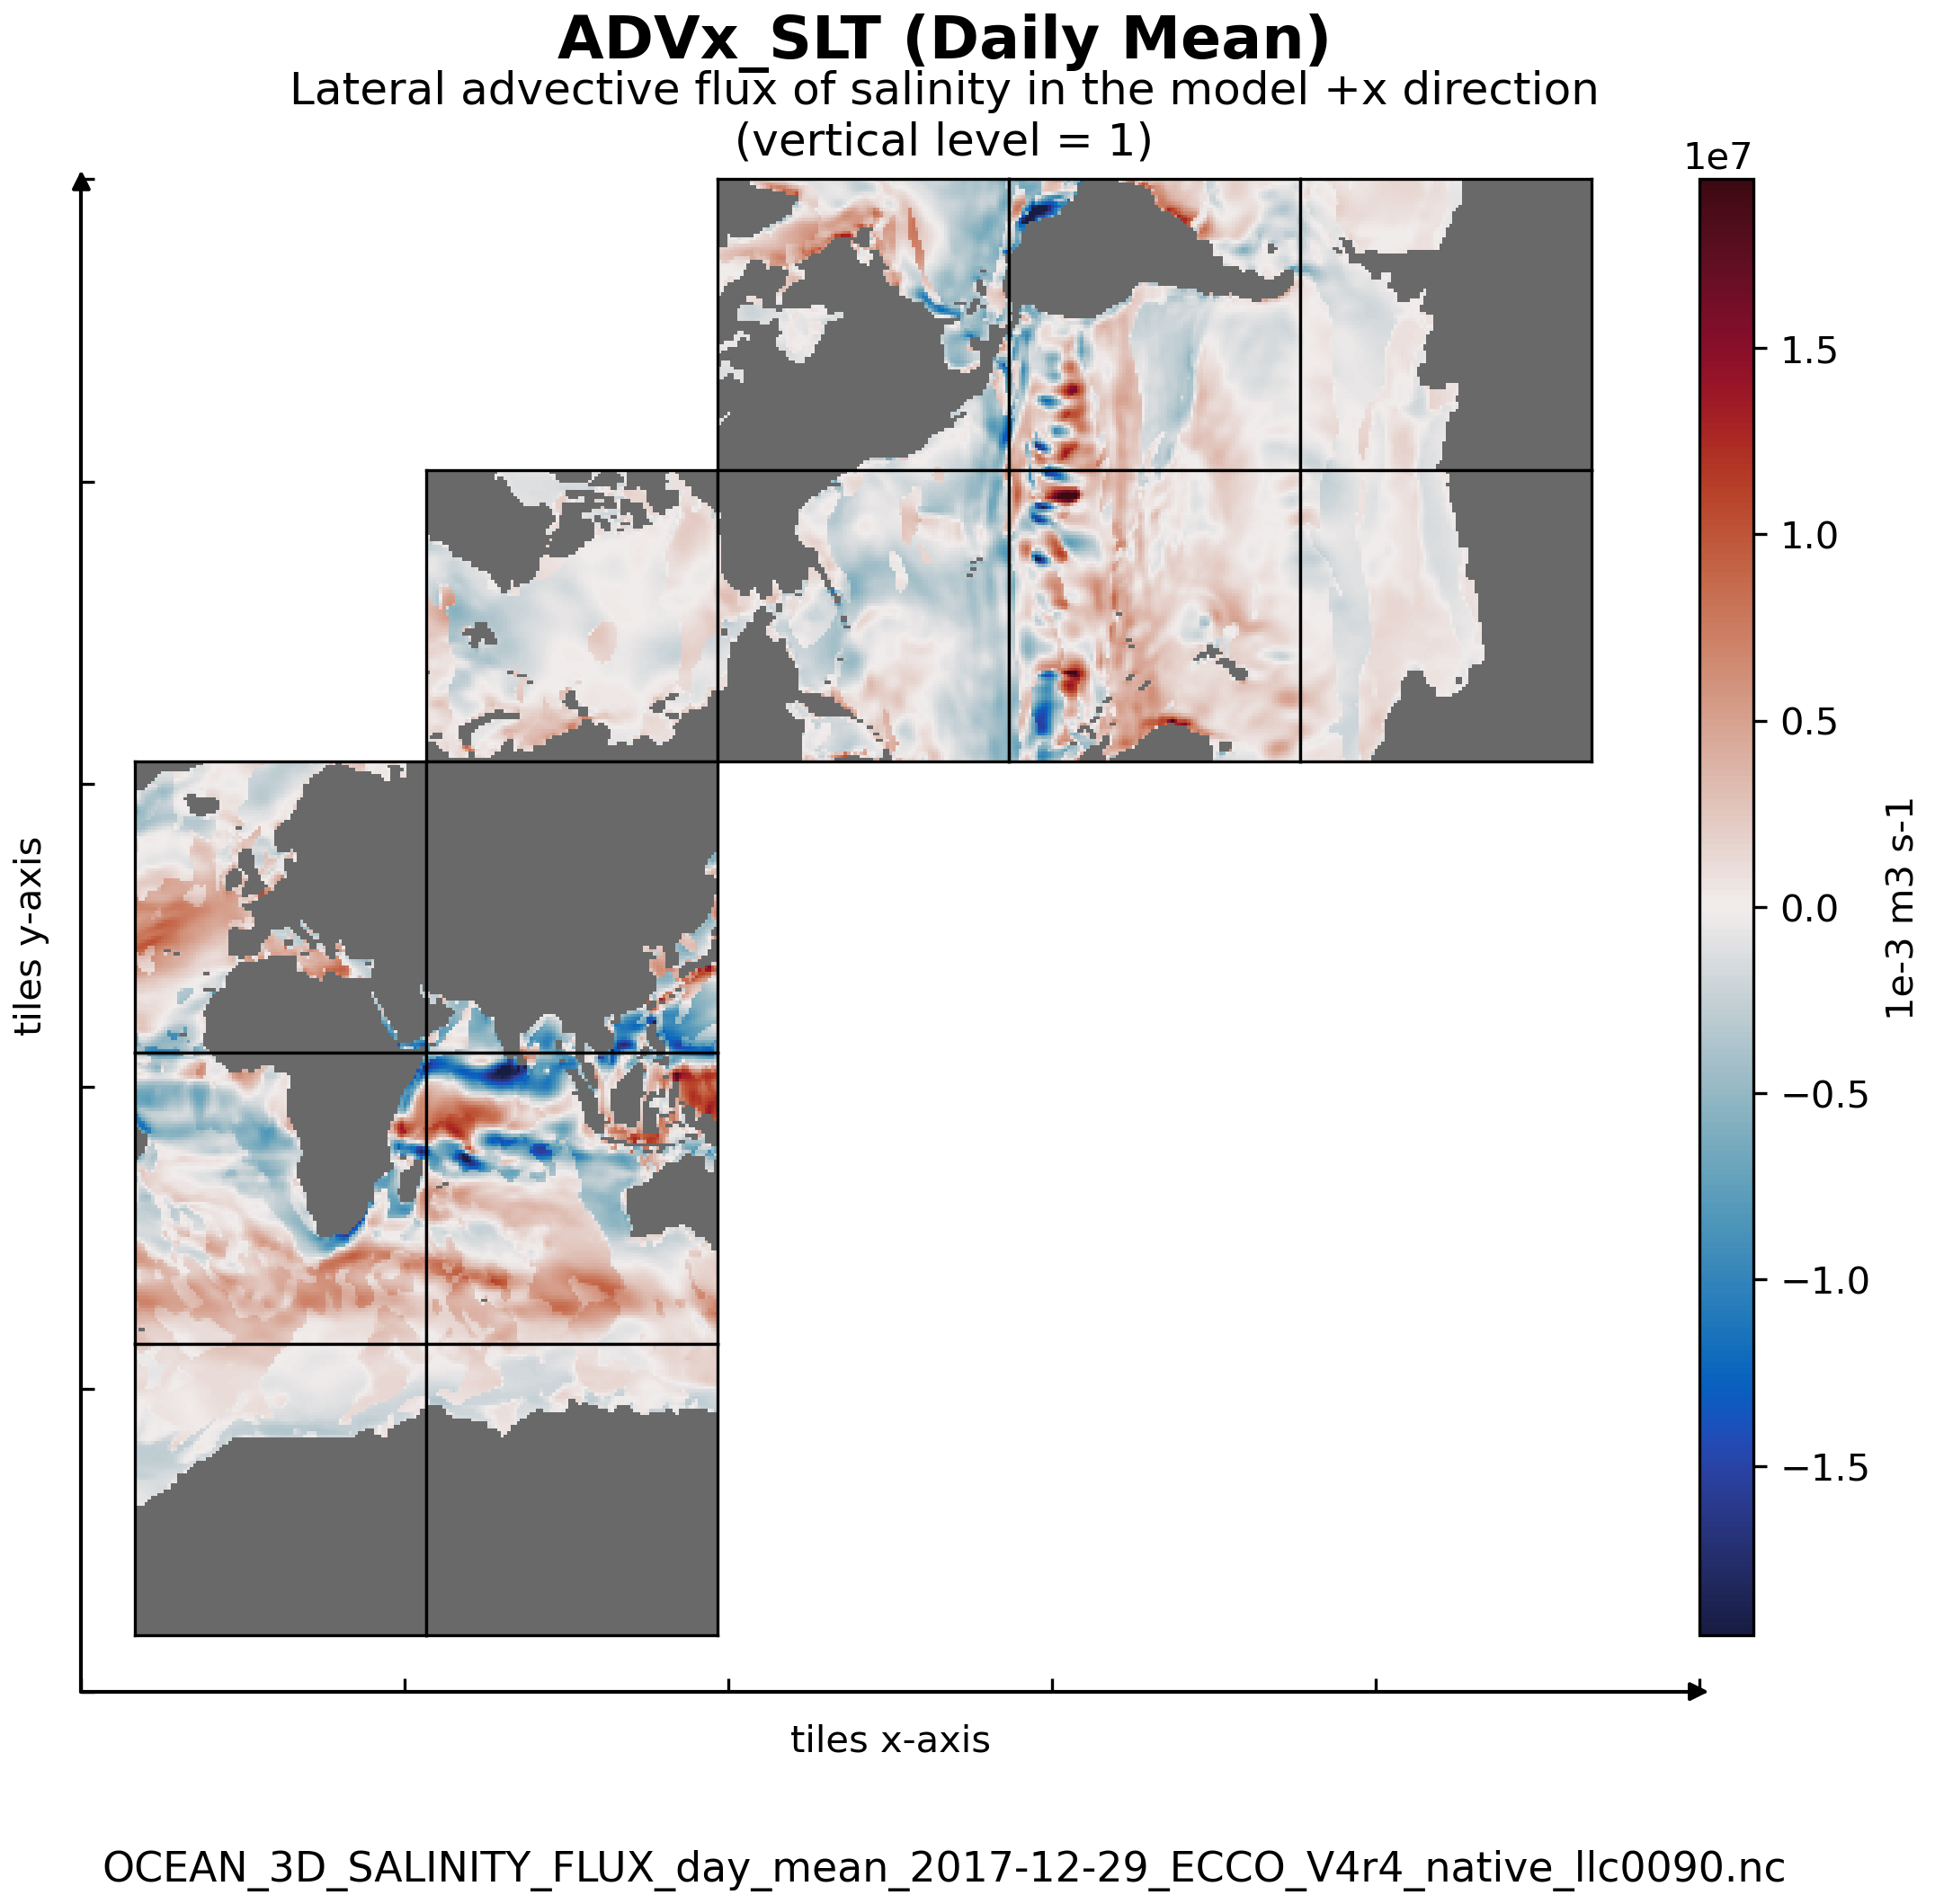
\includegraphics[scale=0.55]{../images/plots/v4r4/native_plots/Ocean_Three-Dimensional_Salinity_Fluxes/ADVx_SLT.png}
\caption{Dataset: OCEAN\_3D\_SALINITY\_FLUX, Variable: ADVx\_SLT}
\label{tab:table-OCEAN_3D_SALINITY_FLUX_ADVx_SLT-Plot}
\end{figure}
\newpage
\pagebreak
\subsubsection{Native Variable: ADVy\_SLT}
\begin{longtable}{|m{0.06\textwidth}|m{0.3\textwidth}|m{0.45\textwidth}|m{0.12\textwidth}|}
\caption{Attributes description of the variable 'ADVy\_SLT' from OCEAN\_3D\_SALINITY\_FLUX's  dataset.}
\label{tab:table-OCEAN_3D_SALINITY_FLUX_ADVy_SLT} \\ 
\hline \endhead \hline \endfoot
\rowcolor{lightgray} \textbf{Storage Type} & \textbf{Variable Name} & \textbf{Description} & \textbf{Unit} \\ \hline
float32 & ADVy\_SLT & Lateral advective flux of salinity in the model +y direction & 1e-3 m3 s-1 \\ \hline
\multicolumn{4}{|c|}{\cellcolor{lightgray}{\textbf{Description of the variable in Common Data language (CDL)}}} \\ \hline
\multicolumn{4}{|c|}{\fontfamily{lmtt}\selectfont{\makecell{\parbox{.95\textwidth}{\vspace*{0.25cm} \footnotesize{float32 ADVy\_SLT(time, k, tile, j\_g, i)\\
\hspace*{0.5cm}ADVy\_SLT: \_FillValue = 9.96921e+36\\
\hspace*{0.5cm}ADVy\_SLT: coordinates = Z time\\
\hspace*{0.5cm}ADVy\_SLT: coverage\_content\_type = modelResult\\
\hspace*{0.5cm}ADVy\_SLT: direction = >0 increases salinity (SALT)\\
\hspace*{0.5cm}ADVy\_SLT: long\_name = Lateral advective flux of salinity in the model +y direction\\
\hspace*{0.5cm}ADVy\_SLT: mate = ADVx SLT\\
\hspace*{0.5cm}ADVy\_SLT: units = 1e-3 m3 s-1\\
\hspace*{0.5cm}ADVy\_SLT: valid\_max = 164271664.0\\
\hspace*{0.5cm}ADVy\_SLT: valid\_min = -137905760.0\\
}}}}} \\ \hline
\rowcolor{lightgray} \multicolumn{4}{|c|}{\textbf{Comments}} \\ \hline
\multicolumn{4}{|p{1\textwidth}|}{\footnotesize{{Lateral advective flux of salinity (salt) in the +y direction through the 'v' face of the tracer cell on the native model grid. note: in the arakawa-c grid, horizontal flux quantities are staggered relative to the tracer cells with indexing such that +advy\_slt(i,j\_g,k) corresponds to +y fluxes through the 'v' face of the tracer cell at (i,j,k). also, the model +y direction does not necessarily correspond to the geographical north-south direction because the x and y axes of the model's curvilinear lat-lon-cap (llc) grid have arbitrary orientations which vary within and across tiles. salinity defined using cf convention 'sea water salinity is the salt content of sea water, often on the practical salinity scale of 1978. however, the unqualified term 'salinity' is generic and does not necessarily imply any particular method of calculation. the units of salinity are dimensionless and the units attribute should normally be given as 1e-3 or 0.001 i.e. parts per thousand.' see https://cfconventions.org/data/cf-standard-names/73/build/cf-standard-name-table.html}}} \\ \hline
\end{longtable}

\begin{figure}[H]
\centering
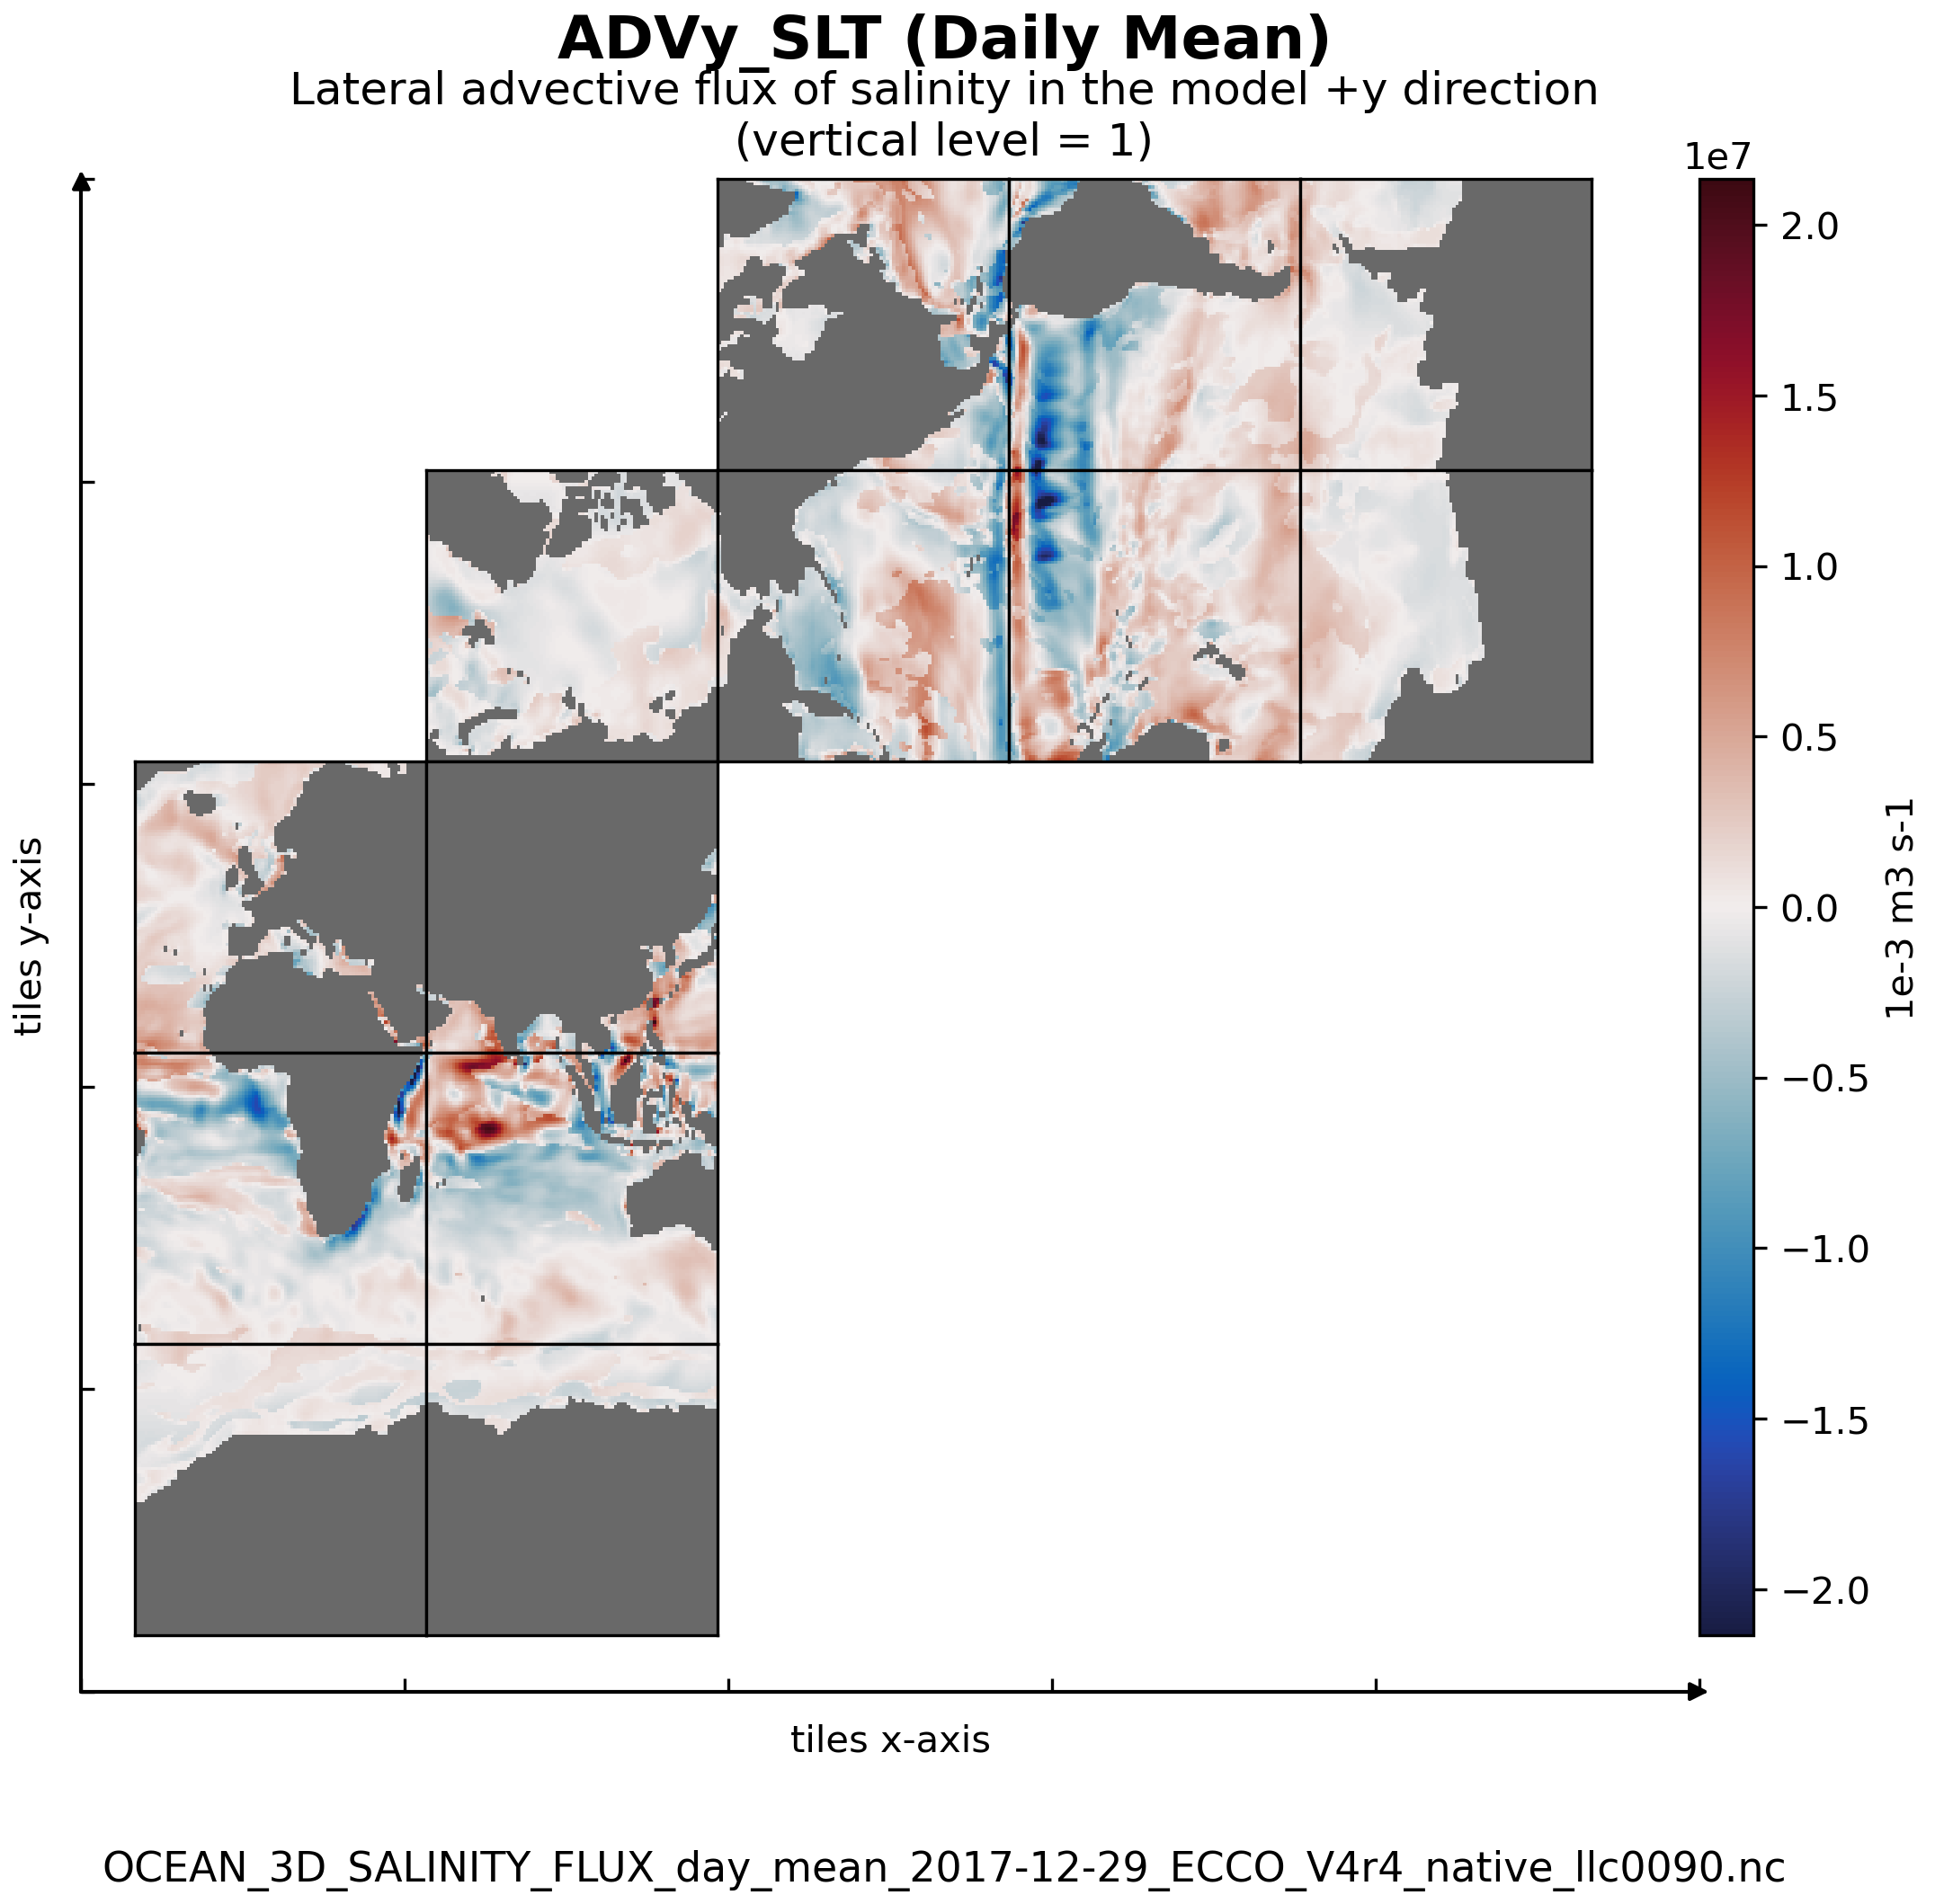
\includegraphics[scale=0.55]{../images/plots/v4r4/native_plots/Ocean_Three-Dimensional_Salinity_Fluxes/ADVy_SLT.png}
\caption{Dataset: OCEAN\_3D\_SALINITY\_FLUX, Variable: ADVy\_SLT}
\label{tab:table-OCEAN_3D_SALINITY_FLUX_ADVy_SLT-Plot}
\end{figure}
\newpage
\pagebreak
\subsubsection{Native Variable: DFrE\_SLT}
\begin{longtable}{|m{0.06\textwidth}|m{0.3\textwidth}|m{0.45\textwidth}|m{0.12\textwidth}|}
\caption{Attributes description of the variable 'DFrE\_SLT' from OCEAN\_3D\_SALINITY\_FLUX's  dataset.}
\label{tab:table-OCEAN_3D_SALINITY_FLUX_DFrE_SLT} \\ 
\hline \endhead \hline \endfoot
\rowcolor{lightgray} \textbf{Storage Type} & \textbf{Variable Name} & \textbf{Description} & \textbf{Unit} \\ \hline
float32 & DFrE\_SLT & Vertical diffusive flux of salinity (explicit term) & 1e-3 m3 s-1 \\ \hline
\multicolumn{4}{|c|}{\cellcolor{lightgray}{\textbf{Description of the variable in Common Data language (CDL)}}} \\ \hline
\multicolumn{4}{|c|}{\fontfamily{lmtt}\selectfont{\makecell{\parbox{.95\textwidth}{\vspace*{0.25cm} \footnotesize{float32 DFrE\_SLT(time, k\_l, tile, j, i)\\
\hspace*{0.5cm}DFrE\_SLT: \_FillValue = 9.96921e+36\\
\hspace*{0.5cm}DFrE\_SLT: coordinates = XC Zl YC time\\
\hspace*{0.5cm}DFrE\_SLT: coverage\_content\_type = modelResult\\
\hspace*{0.5cm}DFrE\_SLT: direction = >0 decreases salinity (SALT)\\
\hspace*{0.5cm}DFrE\_SLT: long\_name = Vertical diffusive flux of salinity (explicit term)\\
\hspace*{0.5cm}DFrE\_SLT: units = 1e-3 m3 s-1\\
\hspace*{0.5cm}DFrE\_SLT: valid\_max = 471215.75\\
\hspace*{0.5cm}DFrE\_SLT: valid\_min = -1074719.375\\
}}}}} \\ \hline
\rowcolor{lightgray} \multicolumn{4}{|c|}{\textbf{Comments}} \\ \hline
\multicolumn{4}{|p{1\textwidth}|}{\footnotesize{{The explicit term of the vertical diffusive flux of salinity (salt) in the +z direction through the top 'w' face of the tracer cell on the native model grid. in the ecco v4r4 model, an implicit scheme is used to calculate vertical diffusive tracer fluxes due to background diffusivity and the kwz component of the gm-redi tensor (vertical flux as a function of vertical gradient) while an explicit scheme is used to calculate the vertical diffusive fluxes from the kwx and kwy components of the gm-redi tensor (vertical flux as a function of horizontal gradient). both implicit and explicit components of vertical diffusive flux of salinity are provided. note: in the arakawa-c grid, vertical flux quantities are staggered relative to the tracer cells with indexing such that +dfre\_slt(i,j,k\_l) corresponds to upward +z fluxes through the top 'w' face of the tracer cell at (i,j,k). salinity defined using cf convention 'sea water salinity is the salt content of sea water, often on the practical salinity scale of 1978. however, the unqualified term 'salinity' is generic and does not necessarily imply any particular method of calculation. the units of salinity are dimensionless and the units attribute should normally be given as 1e-3 or 0.001 i.e. parts per thousand.' see https://cfconventions.org/data/cf-standard-names/73/build/cf-standard-name-table.html}}} \\ \hline
\end{longtable}

\begin{figure}[H]
\centering
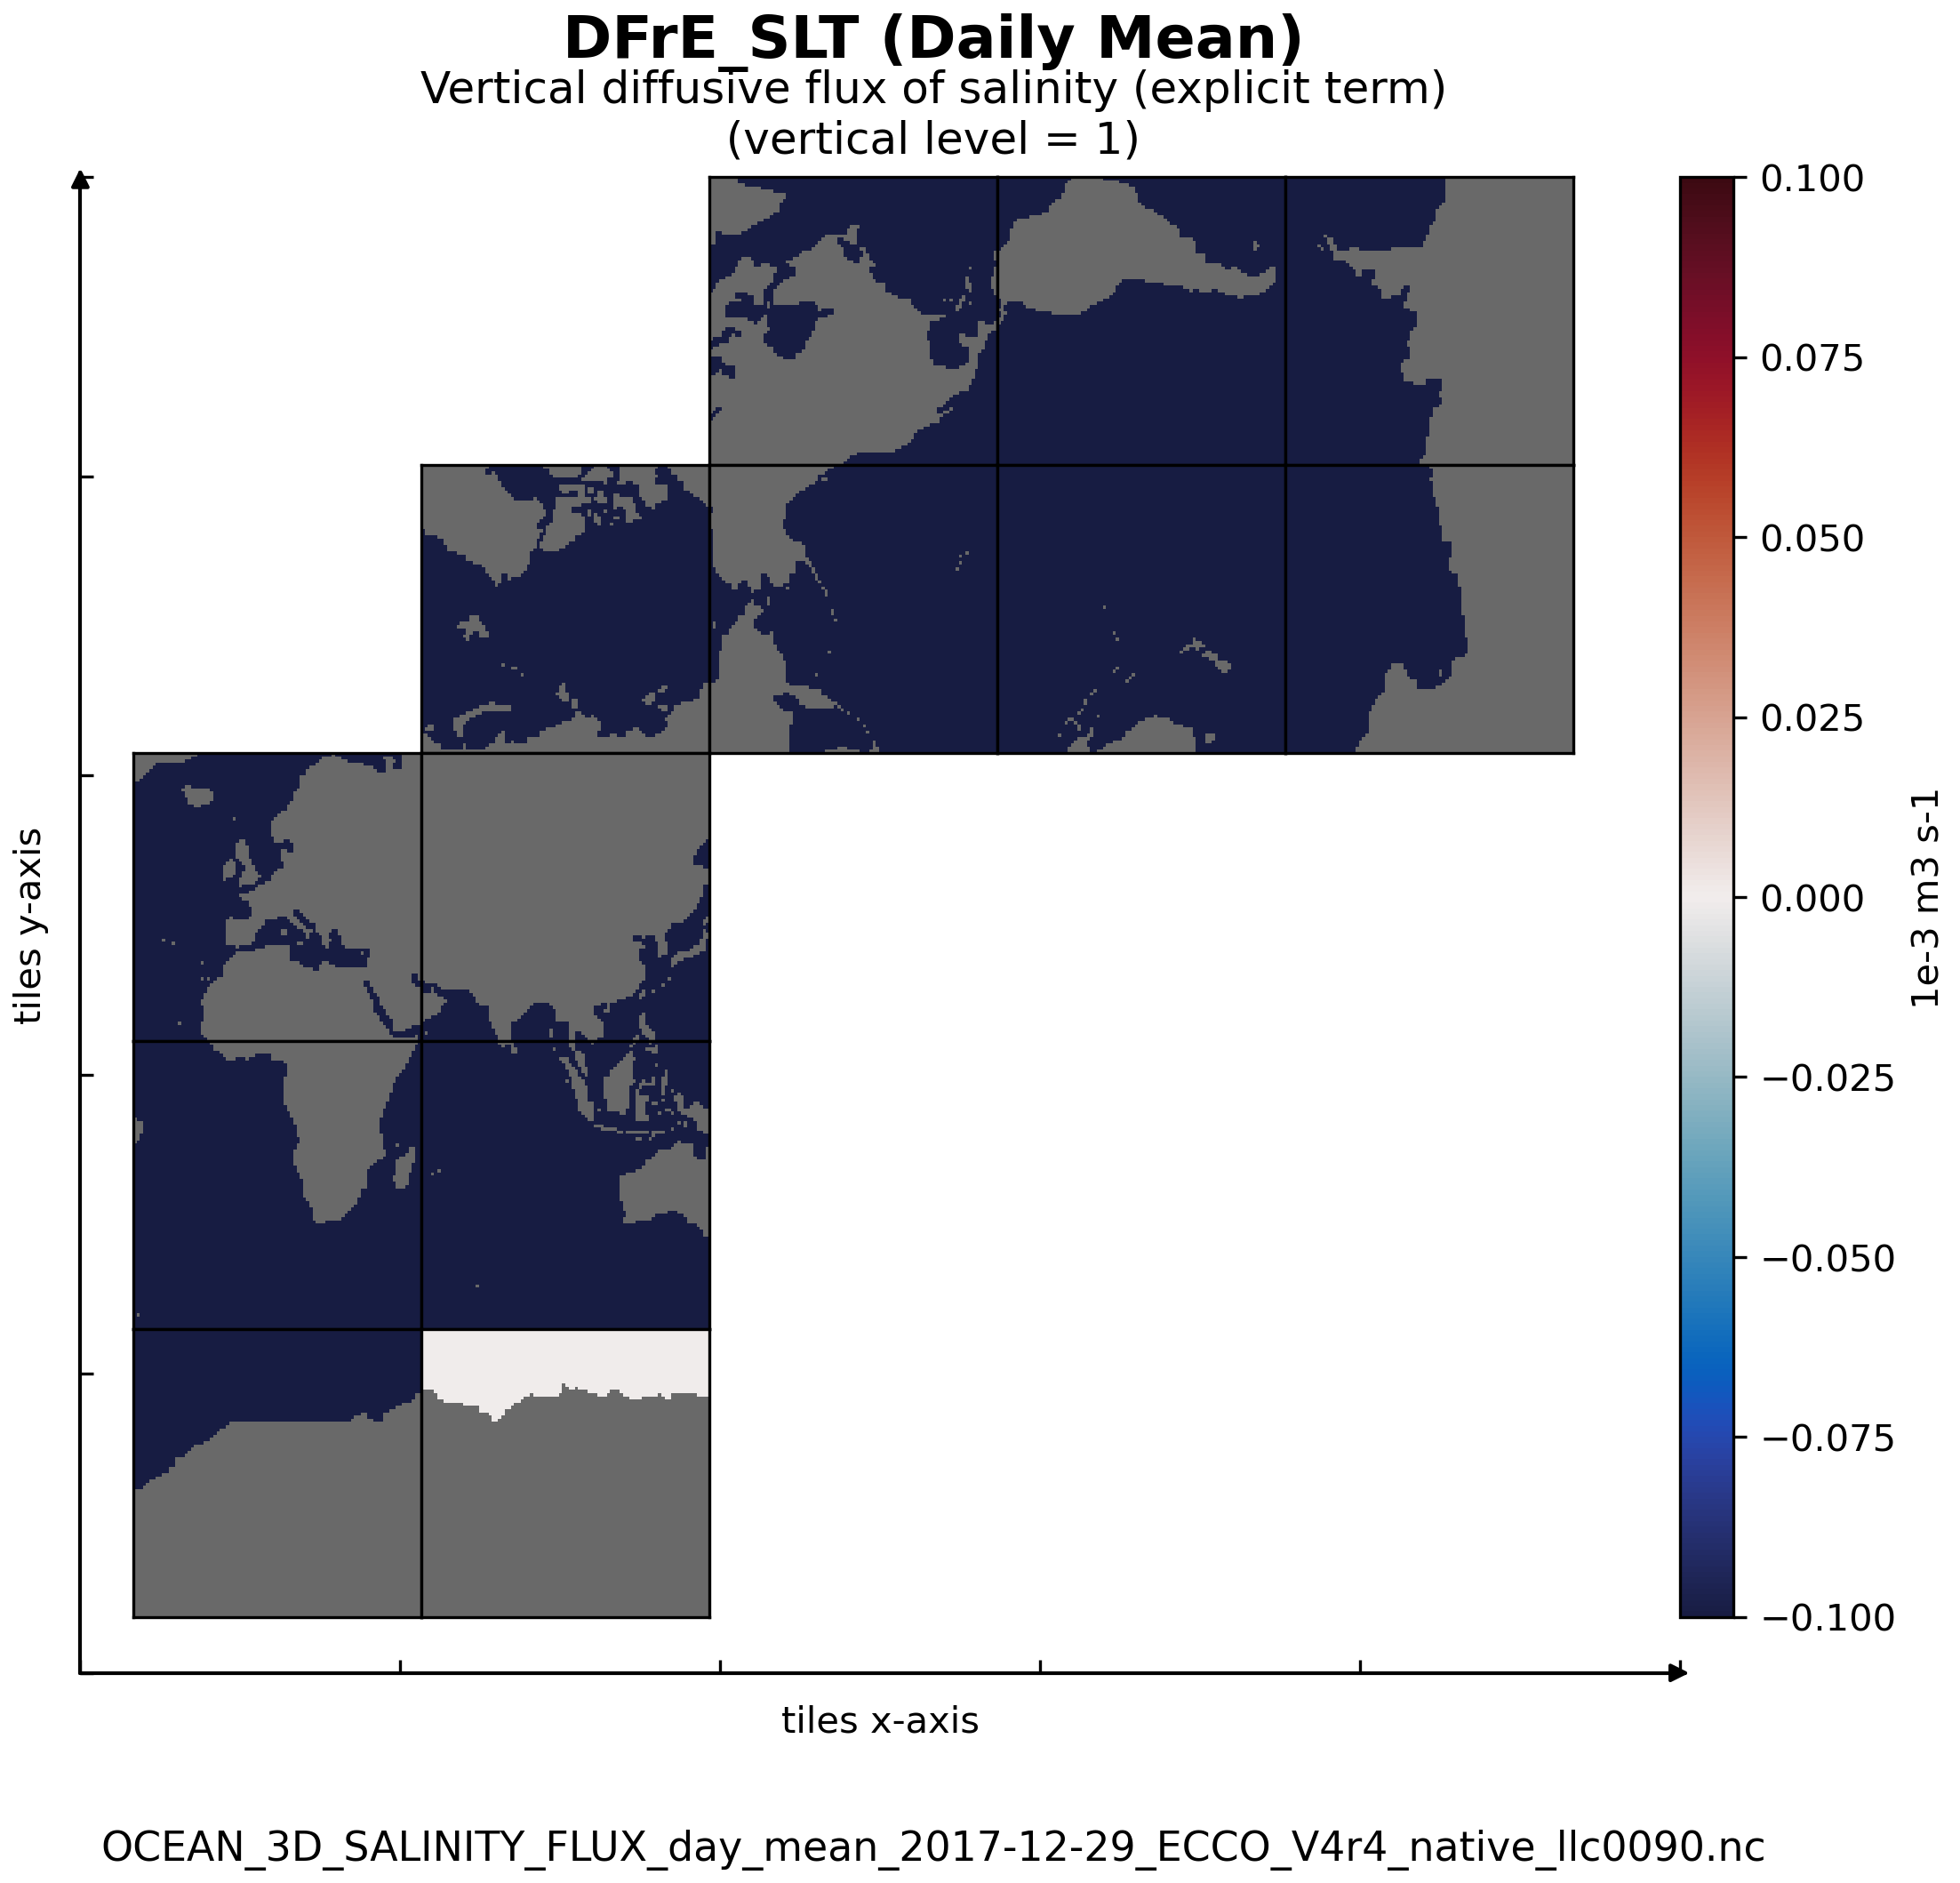
\includegraphics[scale=0.55]{../images/plots/v4r4/native_plots/Ocean_Three-Dimensional_Salinity_Fluxes/DFrE_SLT.png}
\caption{Dataset: OCEAN\_3D\_SALINITY\_FLUX, Variable: DFrE\_SLT}
\label{tab:table-OCEAN_3D_SALINITY_FLUX_DFrE_SLT-Plot}
\end{figure}
\newpage
\pagebreak
\subsubsection{Native Variable: DFrI\_SLT}
\begin{longtable}{|m{0.06\textwidth}|m{0.3\textwidth}|m{0.45\textwidth}|m{0.12\textwidth}|}
\caption{Attributes description of the variable 'DFrI\_SLT' from OCEAN\_3D\_SALINITY\_FLUX's  dataset.}
\label{tab:table-OCEAN_3D_SALINITY_FLUX_DFrI_SLT} \\ 
\hline \endhead \hline \endfoot
\rowcolor{lightgray} \textbf{Storage Type} & \textbf{Variable Name} & \textbf{Description} & \textbf{Unit} \\ \hline
float32 & DFrI\_SLT & Vertical diffusive flux of salinity (implicit term) & 1e-3 m3 s-1 \\ \hline
\multicolumn{4}{|c|}{\cellcolor{lightgray}{\textbf{Description of the variable in Common Data language (CDL)}}} \\ \hline
\multicolumn{4}{|c|}{\fontfamily{lmtt}\selectfont{\makecell{\parbox{.95\textwidth}{\vspace*{0.25cm} \footnotesize{float32 DFrI\_SLT(time, k\_l, tile, j, i)\\
\hspace*{0.5cm}DFrI\_SLT: \_FillValue = 9.96921e+36\\
\hspace*{0.5cm}DFrI\_SLT: coordinates = XC Zl YC time\\
\hspace*{0.5cm}DFrI\_SLT: coverage\_content\_type = modelResult\\
\hspace*{0.5cm}DFrI\_SLT: direction = >0 decreases salinity (SALT)\\
\hspace*{0.5cm}DFrI\_SLT: long\_name = Vertical diffusive flux of salinity (implicit term)\\
\hspace*{0.5cm}DFrI\_SLT: units = 1e-3 m3 s-1\\
\hspace*{0.5cm}DFrI\_SLT: valid\_max = 3197643.0\\
\hspace*{0.5cm}DFrI\_SLT: valid\_min = -30609048.0\\
}}}}} \\ \hline
\rowcolor{lightgray} \multicolumn{4}{|c|}{\textbf{Comments}} \\ \hline
\multicolumn{4}{|p{1\textwidth}|}{\footnotesize{{The implicit term of the vertical diffusive flux of salinity (salt) in the +z direction through the top 'w' face of the tracer cell on the native model grid. in the ecco v4r4 model, an implicit scheme is used to calculate vertical diffusive tracer fluxes due to background diffusivity and the kwz component of the gm-redi tensor (vertical flux as a function of vertical gradient) while an explicit scheme is used to calculate the vertical diffusive fluxes from the kwx and kwy components of the gm-redi tensor (vertical flux as a function of horizontal gradient). both implicit and explicit components of vertical diffusive flux of salinity are provided. note: in the arakawa-c grid, vertical flux quantities are staggered relative to the tracer cells with indexing such that +dfri\_slt(i,j,k\_l) corresponds to upward +z fluxes through the top face 'w' of the tracer cell at (i,j,k). salinity defined using cf convention 'sea water salinity is the salt content of sea water, often on the practical salinity scale of 1978. however, the unqualified term 'salinity' is generic and does not necessarily imply any particular method of calculation. the units of salinity are dimensionless and the units attribute should normally be given as 1e-3 or 0.001 i.e. parts per thousand.' see https://cfconventions.org/data/cf-standard-names/73/build/cf-standard-name-table.html}}} \\ \hline
\end{longtable}

\begin{figure}[H]
\centering
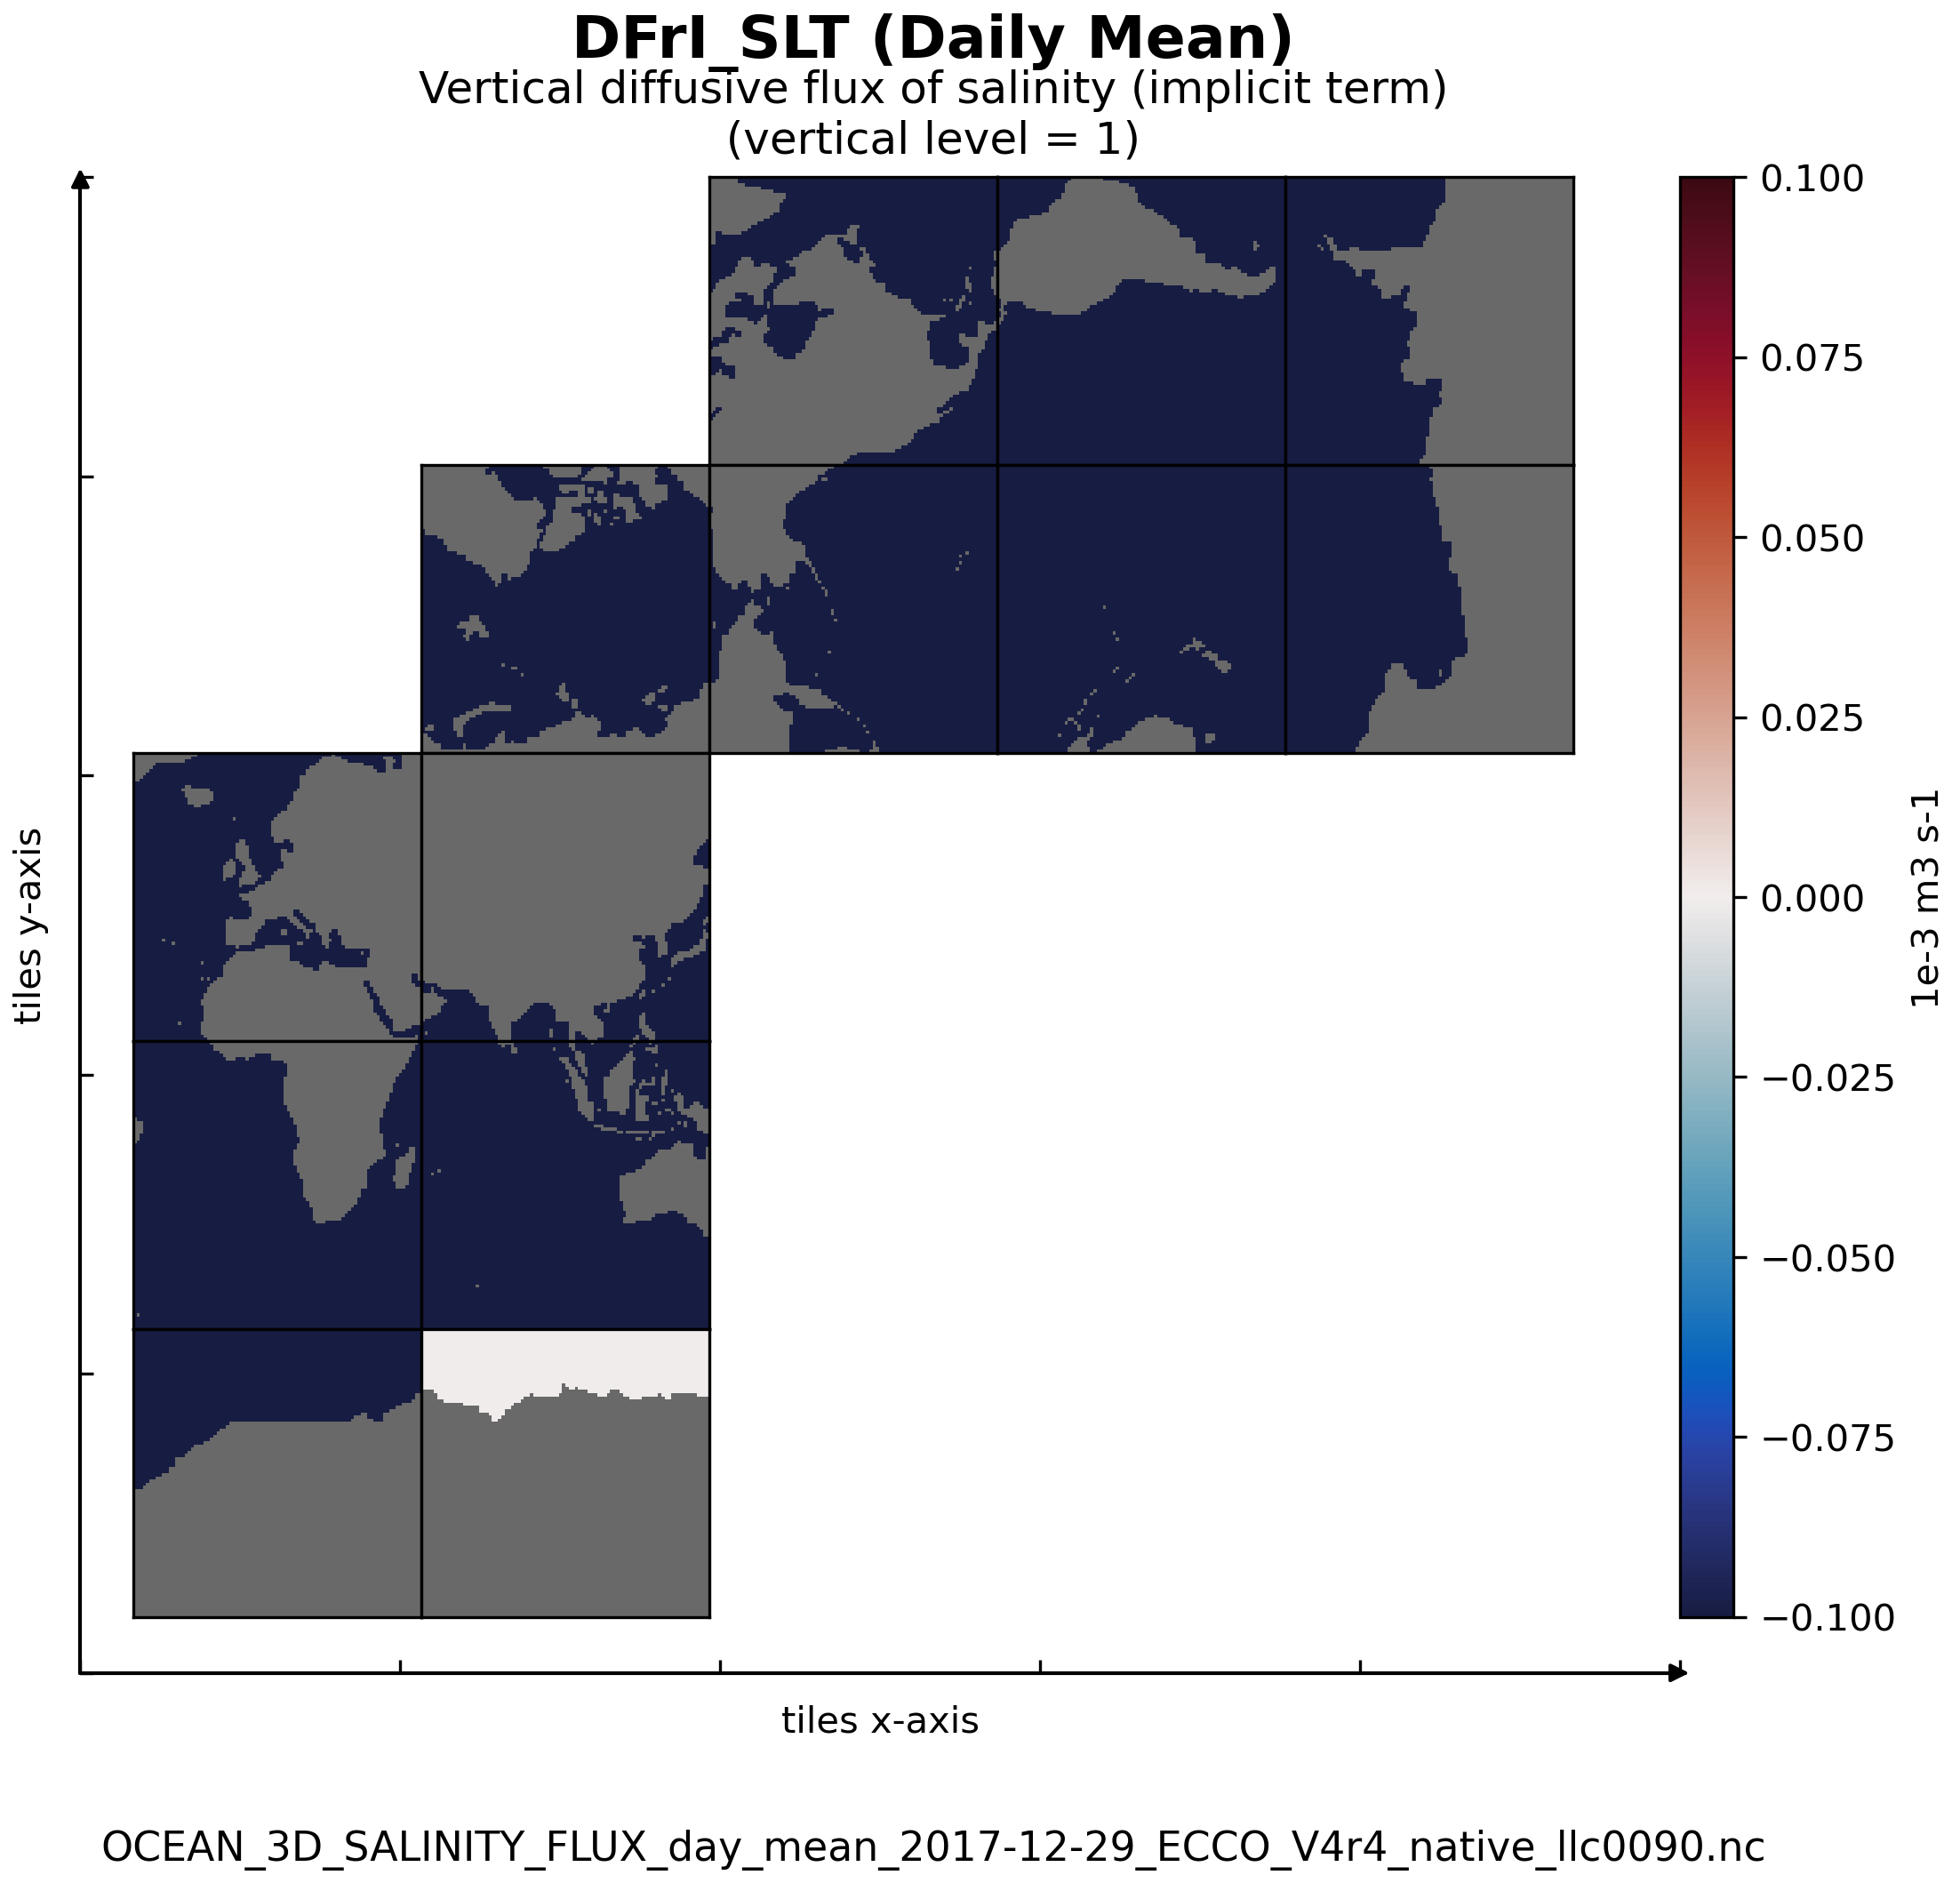
\includegraphics[scale=0.55]{../images/plots/v4r4/native_plots/Ocean_Three-Dimensional_Salinity_Fluxes/DFrI_SLT.png}
\caption{Dataset: OCEAN\_3D\_SALINITY\_FLUX, Variable: DFrI\_SLT}
\label{tab:table-OCEAN_3D_SALINITY_FLUX_DFrI_SLT-Plot}
\end{figure}
\newpage
\pagebreak
\subsubsection{Native Variable: DFxE\_SLT}
\begin{longtable}{|m{0.06\textwidth}|m{0.3\textwidth}|m{0.45\textwidth}|m{0.12\textwidth}|}
\caption{Attributes description of the variable 'DFxE\_SLT' from OCEAN\_3D\_SALINITY\_FLUX's  dataset.}
\label{tab:table-OCEAN_3D_SALINITY_FLUX_DFxE_SLT} \\ 
\hline \endhead \hline \endfoot
\rowcolor{lightgray} \textbf{Storage Type} & \textbf{Variable Name} & \textbf{Description} & \textbf{Unit} \\ \hline
float32 & DFxE\_SLT & Lateral diffusive flux of salinity in the model +x direction & 1e-3 m3 s-1 \\ \hline
\multicolumn{4}{|c|}{\cellcolor{lightgray}{\textbf{Description of the variable in Common Data language (CDL)}}} \\ \hline
\multicolumn{4}{|c|}{\fontfamily{lmtt}\selectfont{\makecell{\parbox{.95\textwidth}{\vspace*{0.25cm} \footnotesize{float32 DFxE\_SLT(time, k, tile, j, i\_g)\\
\hspace*{0.5cm}DFxE\_SLT: \_FillValue = 9.96921e+36\\
\hspace*{0.5cm}DFxE\_SLT: coordinates = Z time\\
\hspace*{0.5cm}DFxE\_SLT: coverage\_content\_type = modelResult\\
\hspace*{0.5cm}DFxE\_SLT: direction = >0 increases salinity (SALT)\\
\hspace*{0.5cm}DFxE\_SLT: long\_name = Lateral diffusive flux of salinity in the model +x direction\\
\hspace*{0.5cm}DFxE\_SLT: mate = DFyE SLT\\
\hspace*{0.5cm}DFxE\_SLT: units = 1e-3 m3 s-1\\
\hspace*{0.5cm}DFxE\_SLT: valid\_max = 192716.484375\\
\hspace*{0.5cm}DFxE\_SLT: valid\_min = -125908.03125\\
}}}}} \\ \hline
\rowcolor{lightgray} \multicolumn{4}{|c|}{\textbf{Comments}} \\ \hline
\multicolumn{4}{|p{1\textwidth}|}{\footnotesize{{Lateral diffusive flux of salinity (salt) in the +x direction through the 'u' face of the tracer cell on the native model grid. note: in the arakawa-c grid, horizontal flux quantities are staggered relative to the tracer cells with indexing such that +dfxe\_slt(i\_g,j,k) corresponds to +x fluxes through the 'u' face of the tracer cell at (i,j,k). also, the model +x direction does not necessarily correspond to the geographical east-west direction because the x and y axes of the model's curvilinear lat-lon-cap (llc) grid have arbitrary orientations which vary within and across tiles. salinity defined using cf convention 'sea water salinity is the salt content of sea water, often on the practical salinity scale of 1978. however, the unqualified term 'salinity' is generic and does not necessarily imply any particular method of calculation. the units of salinity are dimensionless and the units attribute should normally be given as 1e-3 or 0.001 i.e. parts per thousand.' see https://cfconventions.org/data/cf-standard-names/73/build/cf-standard-name-table.html}}} \\ \hline
\end{longtable}

\begin{figure}[H]
\centering
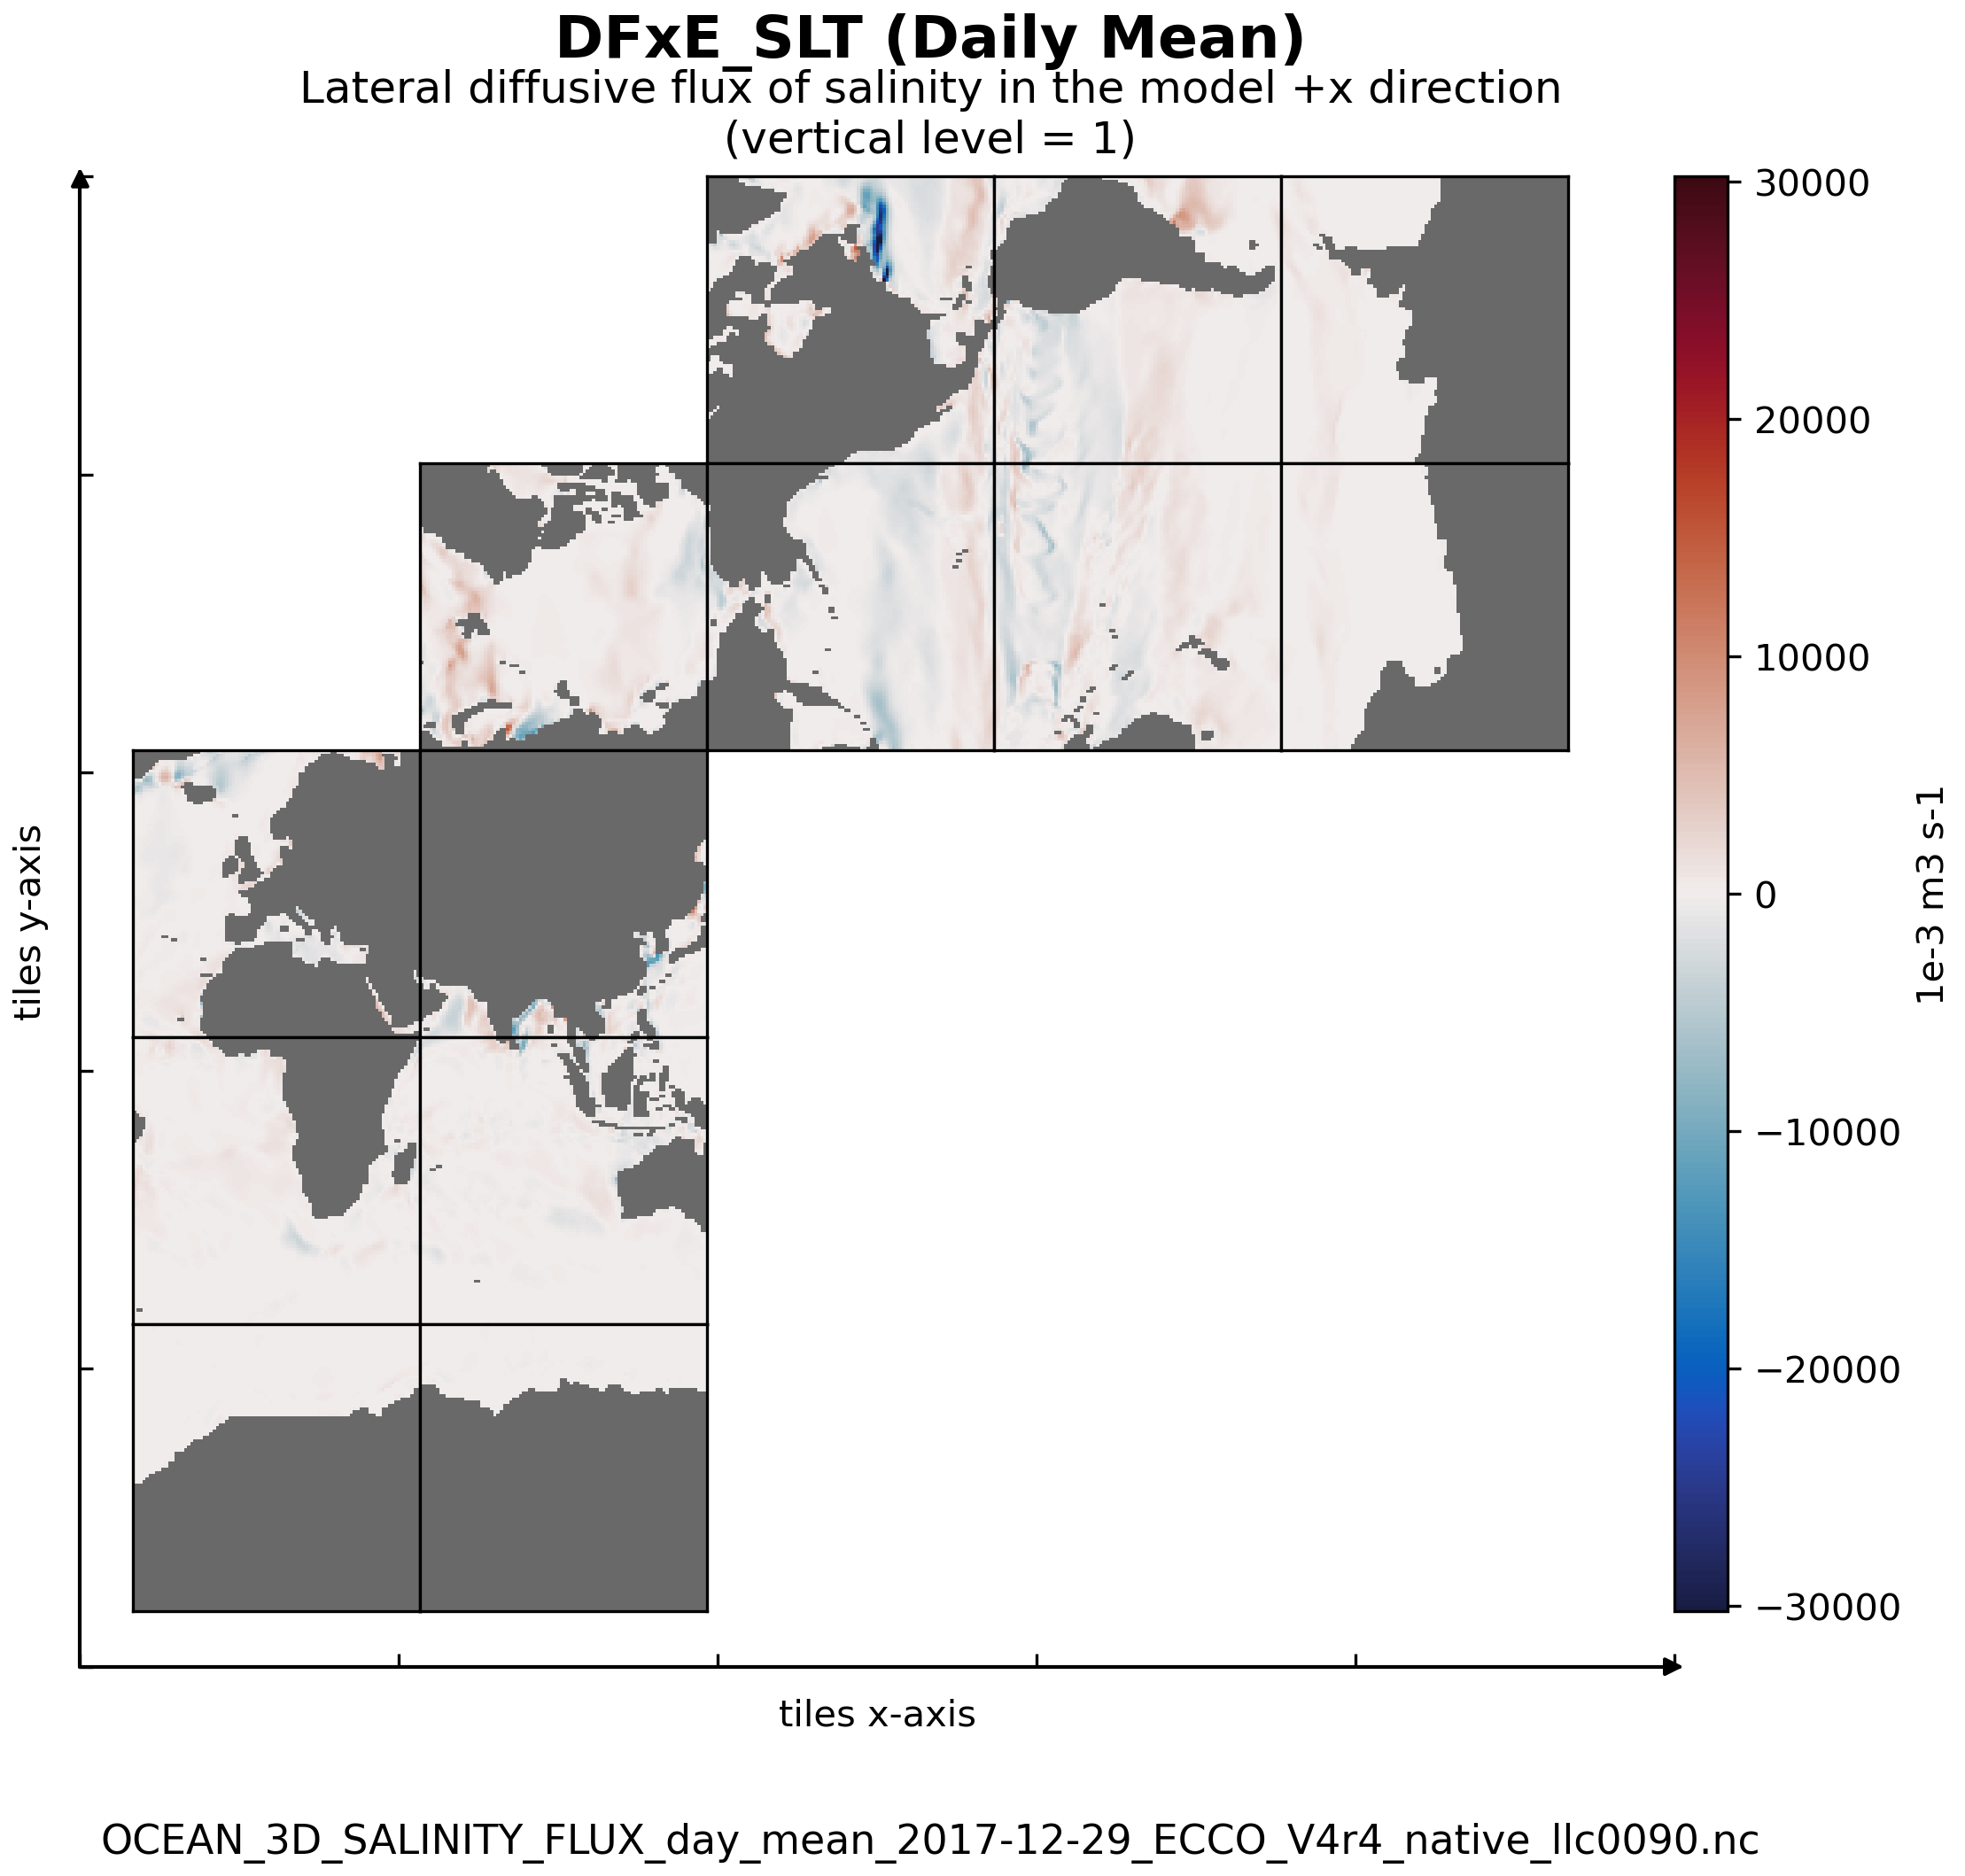
\includegraphics[scale=0.55]{../images/plots/v4r4/native_plots/Ocean_Three-Dimensional_Salinity_Fluxes/DFxE_SLT.png}
\caption{Dataset: OCEAN\_3D\_SALINITY\_FLUX, Variable: DFxE\_SLT}
\label{tab:table-OCEAN_3D_SALINITY_FLUX_DFxE_SLT-Plot}
\end{figure}
\newpage
\pagebreak
\subsubsection{Native Variable: DFyE\_SLT}
\begin{longtable}{|m{0.06\textwidth}|m{0.3\textwidth}|m{0.45\textwidth}|m{0.12\textwidth}|}
\caption{Attributes description of the variable 'DFyE\_SLT' from OCEAN\_3D\_SALINITY\_FLUX's  dataset.}
\label{tab:table-OCEAN_3D_SALINITY_FLUX_DFyE_SLT} \\ 
\hline \endhead \hline \endfoot
\rowcolor{lightgray} \textbf{Storage Type} & \textbf{Variable Name} & \textbf{Description} & \textbf{Unit} \\ \hline
float32 & DFyE\_SLT & Lateral diffusive flux of salinity in the model +y direction & 1e-3 m3 s-1 \\ \hline
\multicolumn{4}{|c|}{\cellcolor{lightgray}{\textbf{Description of the variable in Common Data language (CDL)}}} \\ \hline
\multicolumn{4}{|c|}{\fontfamily{lmtt}\selectfont{\makecell{\parbox{.95\textwidth}{\vspace*{0.25cm} \footnotesize{float32 DFyE\_SLT(time, k, tile, j\_g, i)\\
\hspace*{0.5cm}DFyE\_SLT: \_FillValue = 9.96921e+36\\
\hspace*{0.5cm}DFyE\_SLT: coordinates = Z time\\
\hspace*{0.5cm}DFyE\_SLT: coverage\_content\_type = modelResult\\
\hspace*{0.5cm}DFyE\_SLT: direction = >0 increases salinity (SALT)\\
\hspace*{0.5cm}DFyE\_SLT: long\_name = Lateral diffusive flux of salinity in the model +y direction\\
\hspace*{0.5cm}DFyE\_SLT: mate = DFxE SLT\\
\hspace*{0.5cm}DFyE\_SLT: units = 1e-3 m3 s-1\\
\hspace*{0.5cm}DFyE\_SLT: valid\_max = 154227.140625\\
\hspace*{0.5cm}DFyE\_SLT: valid\_min = -114959.2109375\\
}}}}} \\ \hline
\rowcolor{lightgray} \multicolumn{4}{|c|}{\textbf{Comments}} \\ \hline
\multicolumn{4}{|p{1\textwidth}|}{\footnotesize{{Lateral diffusive flux of salinity (salt) in the +y direction through the 'v' face of the tracer cell on the native model grid. note: in the arakawa-c grid, horizontal flux quantities are staggered relative to the tracer cells with indexing such that +dfye\_slt(i,j\_g,k) corresponds to +y fluxes through the 'v' face of the tracer cell at (i,j,k). also, the model +y direction does not necessarily correspond to the geographical north-south direction because the x and y axes of the model's curvilinear lat-lon-cap (llc) grid have arbitrary orientations which vary within and across tiles. salinity defined using cf convention 'sea water salinity is the salt content of sea water, often on the practical salinity scale of 1978. however, the unqualified term 'salinity' is generic and does not necessarily imply any particular method of calculation. the units of salinity are dimensionless and the units attribute should normally be given as 1e-3 or 0.001 i.e. parts per thousand.' see https://cfconventions.org/data/cf-standard-names/73/build/cf-standard-name-table.html}}} \\ \hline
\end{longtable}

\begin{figure}[H]
\centering
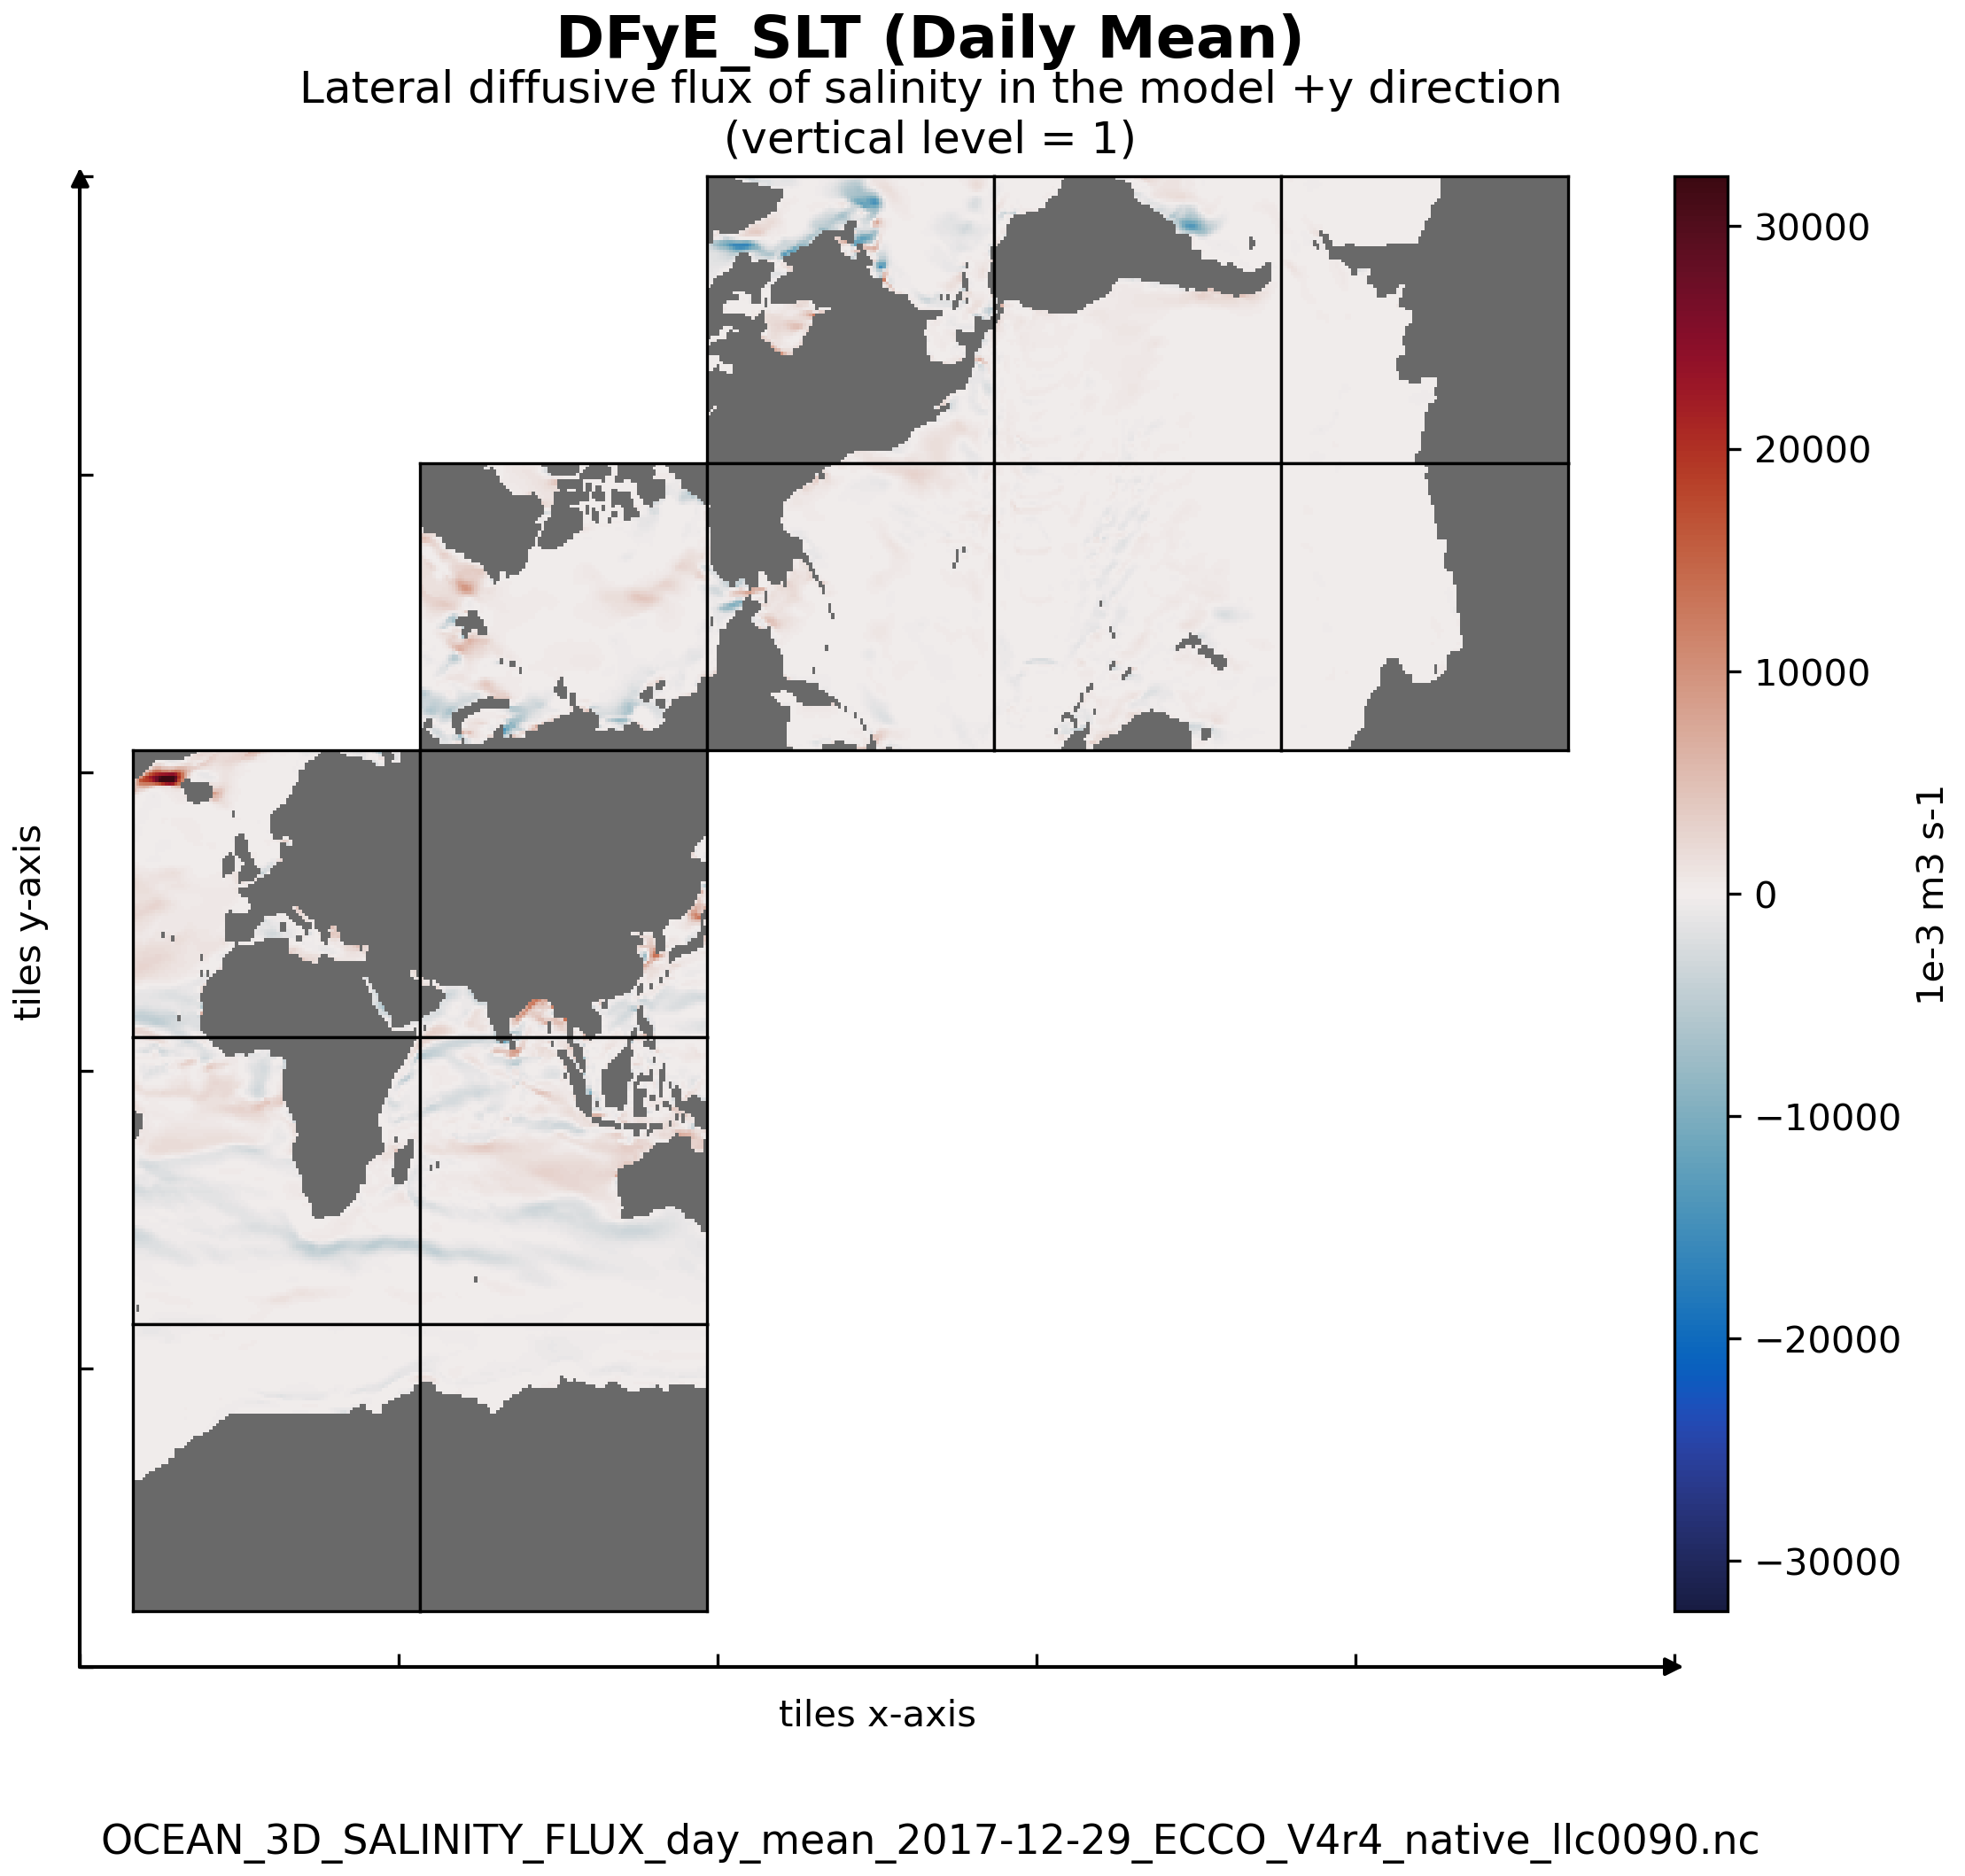
\includegraphics[scale=0.55]{../images/plots/v4r4/native_plots/Ocean_Three-Dimensional_Salinity_Fluxes/DFyE_SLT.png}
\caption{Dataset: OCEAN\_3D\_SALINITY\_FLUX, Variable: DFyE\_SLT}
\label{tab:table-OCEAN_3D_SALINITY_FLUX_DFyE_SLT-Plot}
\end{figure}
\newpage
\pagebreak
\subsubsection{Native Variable: oceSPtnd}
\begin{longtable}{|m{0.06\textwidth}|m{0.3\textwidth}|m{0.45\textwidth}|m{0.12\textwidth}|}
\caption{Attributes description of the variable 'oceSPtnd' from OCEAN\_3D\_SALINITY\_FLUX's  dataset.}
\label{tab:table-OCEAN_3D_SALINITY_FLUX_oceSPtnd} \\ 
\hline \endhead \hline \endfoot
\rowcolor{lightgray} \textbf{Storage Type} & \textbf{Variable Name} & \textbf{Description} & \textbf{Unit} \\ \hline
float32 & oceSPtnd & Salt tendency due to the vertical transport of salt in high-salinity brine plumes & g m-2 s-1 \\ \hline
\multicolumn{4}{|c|}{\cellcolor{lightgray}{\textbf{Description of the variable in Common Data language (CDL)}}} \\ \hline
\multicolumn{4}{|c|}{\fontfamily{lmtt}\selectfont{\makecell{\parbox{.95\textwidth}{\vspace*{0.25cm} \footnotesize{float32 oceSPtnd(time, k, tile, j, i)\\
\hspace*{0.5cm}oceSPtnd: \_FillValue = 9.96921e+36\\
\hspace*{0.5cm}oceSPtnd: coordinates = XC Z YC time\\
\hspace*{0.5cm}oceSPtnd: coverage\_content\_type = modelResult\\
\hspace*{0.5cm}oceSPtnd: direction = >0 increases salinity (SALT)\\
\hspace*{0.5cm}oceSPtnd: long\_name = Salt tendency due to the vertical transport of salt in high-salinity brine plumes\\
\hspace*{0.5cm}oceSPtnd: units = g m-2 s-1\\
\hspace*{0.5cm}oceSPtnd: valid\_max = 0.021119138225913048\\
\hspace*{0.5cm}oceSPtnd: valid\_min = 0.0\\
}}}}} \\ \hline
\rowcolor{lightgray} \multicolumn{4}{|c|}{\textbf{Comments}} \\ \hline
\multicolumn{4}{|p{1\textwidth}|}{\footnotesize{{Salt tendency due to the vertical transport of salt in high-salinity brine plumes. note: units are grams of salt per square meter per second, not salinity per square meter per second.}}} \\ \hline
\end{longtable}

\begin{figure}[H]
\centering
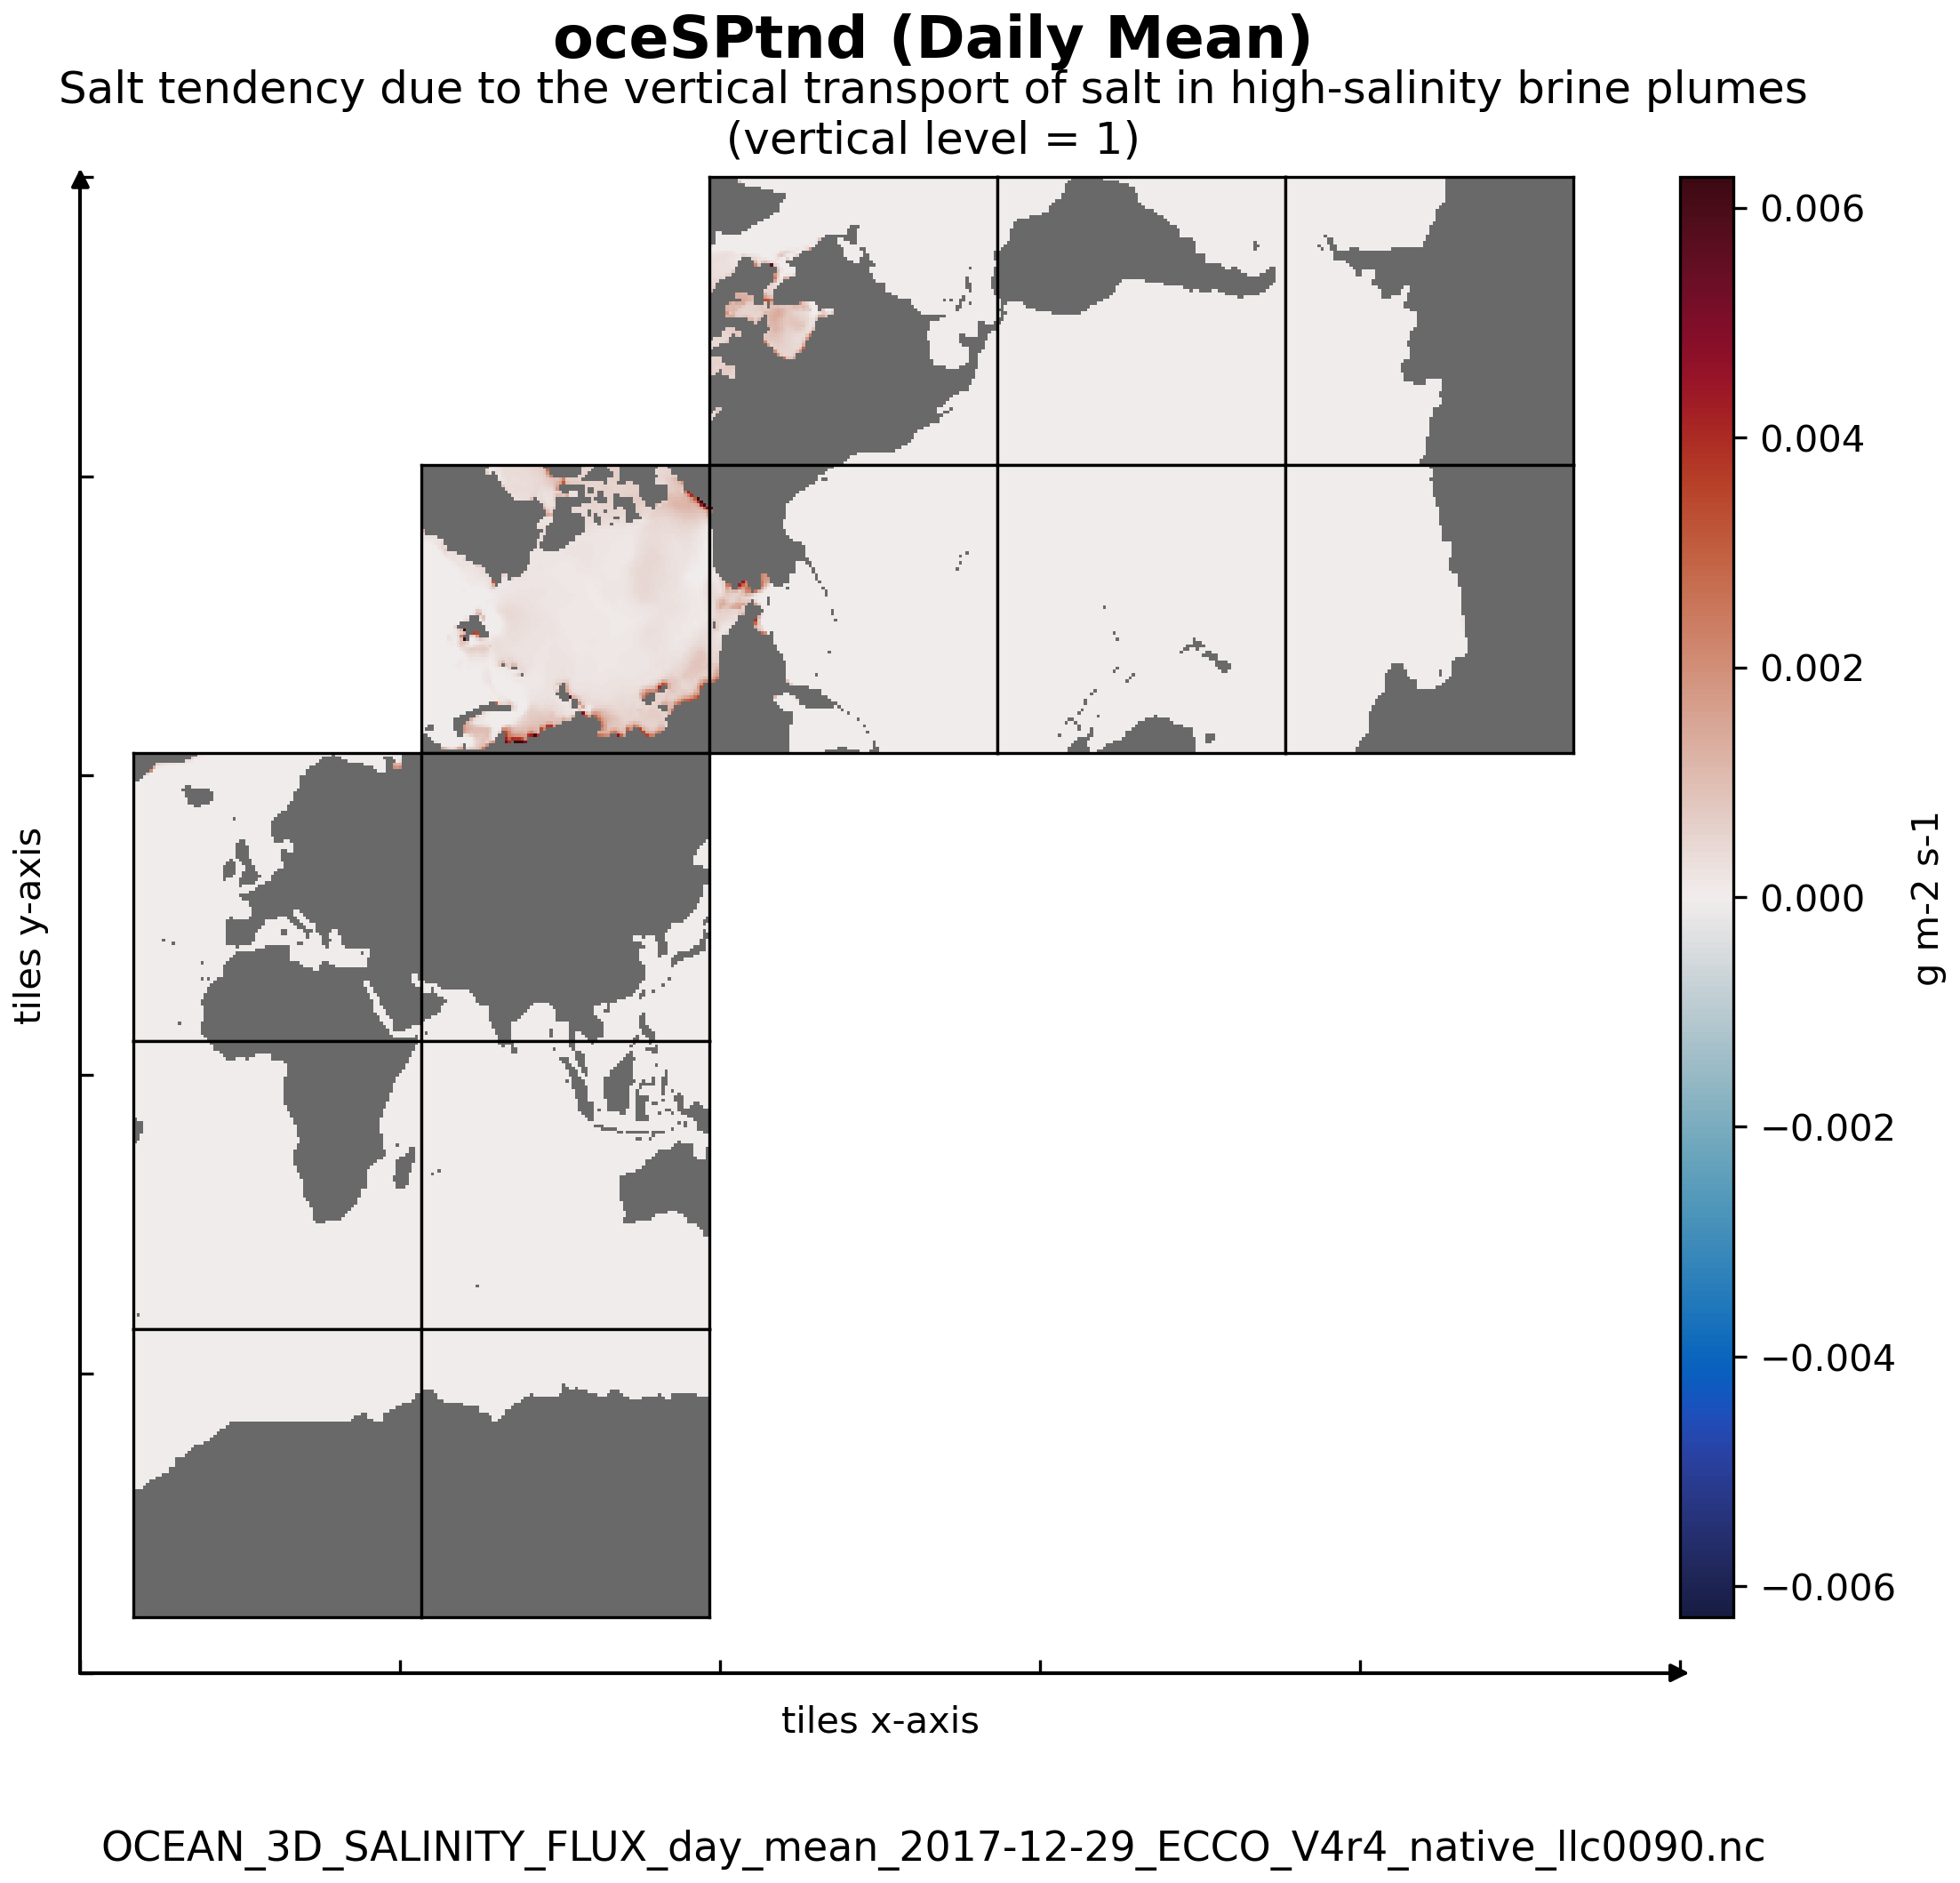
\includegraphics[scale=0.55]{../images/plots/v4r4/native_plots/Ocean_Three-Dimensional_Salinity_Fluxes/oceSPtnd.png}
\caption{Dataset: OCEAN\_3D\_SALINITY\_FLUX, Variable: oceSPtnd}
\label{tab:table-OCEAN_3D_SALINITY_FLUX_oceSPtnd-Plot}
\end{figure}
\newpage
\subsection{Native dataset of OCEAN\_3D\_TEMPERATURE\_FLUX}
\newp
\subsubsection{Overview}
This dataset provides three-dimensional ocean potential temperature fluxes on the lat-lon-cap 90 (llc90) native model grid from the ECCO Version 4 Release 4 (V4r4) ocean and sea-ice state estimate. The dataset is provided on daily-average and monthly-average time resolution. ADV*\_TH and DF*\_TH terms are potential temperature fluxes. 
\begin{longtable}{|m{0.15\textwidth}|m{0.64\textwidth}|m{0.12\textwidth}|}
\caption{Coordinates and Variables in the dataset OCEAN\_3D\_TEMPERATURE\_FLUX}
\label{tab:table-OCEAN_3D_TEMPERATURE_FLUX-fields} \\ 
\hline \endhead \hline \endfoot
\rowcolor{lightgray} \multicolumn{1}{|c|}{\textbf{Coordinates}} & \multicolumn{1}{|c|}{\textbf{Description of data coordinates}} &  \multicolumn{1}{|c|}{\textbf{Unit}}\\ \hline
i &Grid index in x for variables at tracer and 'v' locations &--none--  \\ \hline
i\_g &Grid index in x for variables at 'u' and 'g' locations &--none--  \\ \hline
j &Grid index in y for variables at tracer and 'u' locations &--none--  \\ \hline
j\_g &Grid index in y for variables at 'v' and 'g' locations &--none--  \\ \hline
k &Grid index in z for tracer variables &--none--  \\ \hline
k\_u &Grid index in z corresponding to the bottom face of tracer grid cells ('w' locations) &--none--  \\ \hline
k\_l &Grid index in z corresponding to the top face of tracer grid cells ('w' locations) &--none--  \\ \hline
k\_p1 &Grid index in z for variables at 'w' locations &--none--  \\ \hline
tile &Lat-lon-cap tile index &--none--  \\ \hline
time &Center time of averaging period &--none--  \\ \hline
XC &Longitude of tracer grid cell center &degrees\_east  \\ \hline
YC &Latitude of tracer grid cell center &degrees\_north  \\ \hline
XG &Longitude of 'southwest' corner of tracer grid cell &degrees\_east  \\ \hline
YG &Latitude of 'southwest' corner of tracer grid cell &degrees\_north  \\ \hline
Z &Depth of tracer grid cell center &m  \\ \hline
Zp1 &Depth of tracer grid cell interface &m  \\ \hline
Zu &Depth of the bottom face of tracer grid cells &m  \\ \hline
Zl &Depth of the top face of tracer grid cells &m  \\ \hline
time\_bnds &Time bounds of averaging period &--none--  \\ \hline
XC\_bnds &Longitudes of tracer grid cell corners &--none--  \\ \hline
YC\_bnds &Latitudes of tracer grid cell corners &--none--  \\ \hline
Z\_bnds &Depths of tracer grid cell upper and lower interfaces &--none--  \\ \hline
\rowcolor{lightgray} \multicolumn{1}{|c|}{\textbf{Variables}} & \multicolumn{1}{|c|}{\textbf{Description of data variables}} &  \multicolumn{1}{|c|}{\textbf{Unit}}\\ \hline
ADVx\_TH &Lateral advective flux of potential temperature in the model +x direction &degree\_C m3 s-1  \\ \hline
DFxE\_TH &Lateral diffusive flux of potential temperature in the model +x direction &degree\_C m3 s-1  \\ \hline
ADVy\_TH &Lateral advective flux of potential temperature in the model +y direction &degree\_C m3 s-1  \\ \hline
DFyE\_TH &Lateral diffusive flux of potential temperature in the model +y direction. &degree\_C m3 s-1  \\ \hline
ADVr\_TH &Vertical advective flux of potential temperature &degree\_C m3 s-1  \\ \hline
DFrE\_TH &Vertical diffusive flux of potential temperature (explicit term) &degree\_C m3 s-1  \\ \hline
DFrI\_TH &Vertical diffusive flux of potential temperature (implicit term) &degree\_C m3 s-1  \\ \hline
\end{longtable}

\newp
\pagebreak
\subsubsection{Native Variable: ADVr\_TH}
\begin{longtable}{|m{0.06\textwidth}|m{0.3\textwidth}|m{0.45\textwidth}|m{0.12\textwidth}|}
\caption{Attributes description of the variable 'ADVr\_TH' from OCEAN\_3D\_TEMPERATURE\_FLUX's  dataset.}
\label{tab:table-OCEAN_3D_TEMPERATURE_FLUX_ADVr_TH} \\ 
\hline \endhead \hline \endfoot
\rowcolor{lightgray} \textbf{Storage Type} & \textbf{Variable Name} & \textbf{Description} & \textbf{Unit} \\ \hline
float32 & ADVr\_TH & Vertical advective flux of potential temperature & degree\_C m3 s-1 \\ \hline
\multicolumn{4}{|c|}{\cellcolor{lightgray}{\textbf{Description of the variable in Common Data language (CDL)}}} \\ \hline
\multicolumn{4}{|c|}{\fontfamily{lmtt}\selectfont{\makecell{\parbox{.95\textwidth}{\vspace*{0.25cm} \footnotesize{float32 ADVr\_TH(time, k\_l, tile, j, i)\\
\hspace*{0.5cm}ADVr\_TH: \_FillValue = 9.96921e+36\\
\hspace*{0.5cm}ADVr\_TH: coordinates = XC YC time Zl\\
\hspace*{0.5cm}ADVr\_TH: coverage\_content\_type = modelResult\\
\hspace*{0.5cm}ADVr\_TH: direction = >0 decreases potential temperature (THETA)\\
\hspace*{0.5cm}ADVr\_TH: long\_name = Vertical advective flux of potential temperature\\
\hspace*{0.5cm}ADVr\_TH: units = degree C m3 s-1\\
\hspace*{0.5cm}ADVr\_TH: valid\_max = 179459344.0\\
\hspace*{0.5cm}ADVr\_TH: valid\_min = -125094904.0\\
}}}}} \\ \hline
\rowcolor{lightgray} \multicolumn{4}{|c|}{\textbf{Comments}} \\ \hline
\multicolumn{4}{|p{1\textwidth}|}{\footnotesize{{Vertical advective flux of potential temperature (theta) in the +z direction through the top 'w' face of the tracer cell on the native model grid. note: in the arakawa-c grid, vertical flux quantities are staggered relative to the tracer cells with indexing such that +advr\_th(i,j,k\_l) corresponds to upward +z fluxes through the top 'w' face of the tracer cell at (i,j,k)}}} \\ \hline
\end{longtable}

\begin{figure}[H]
\centering
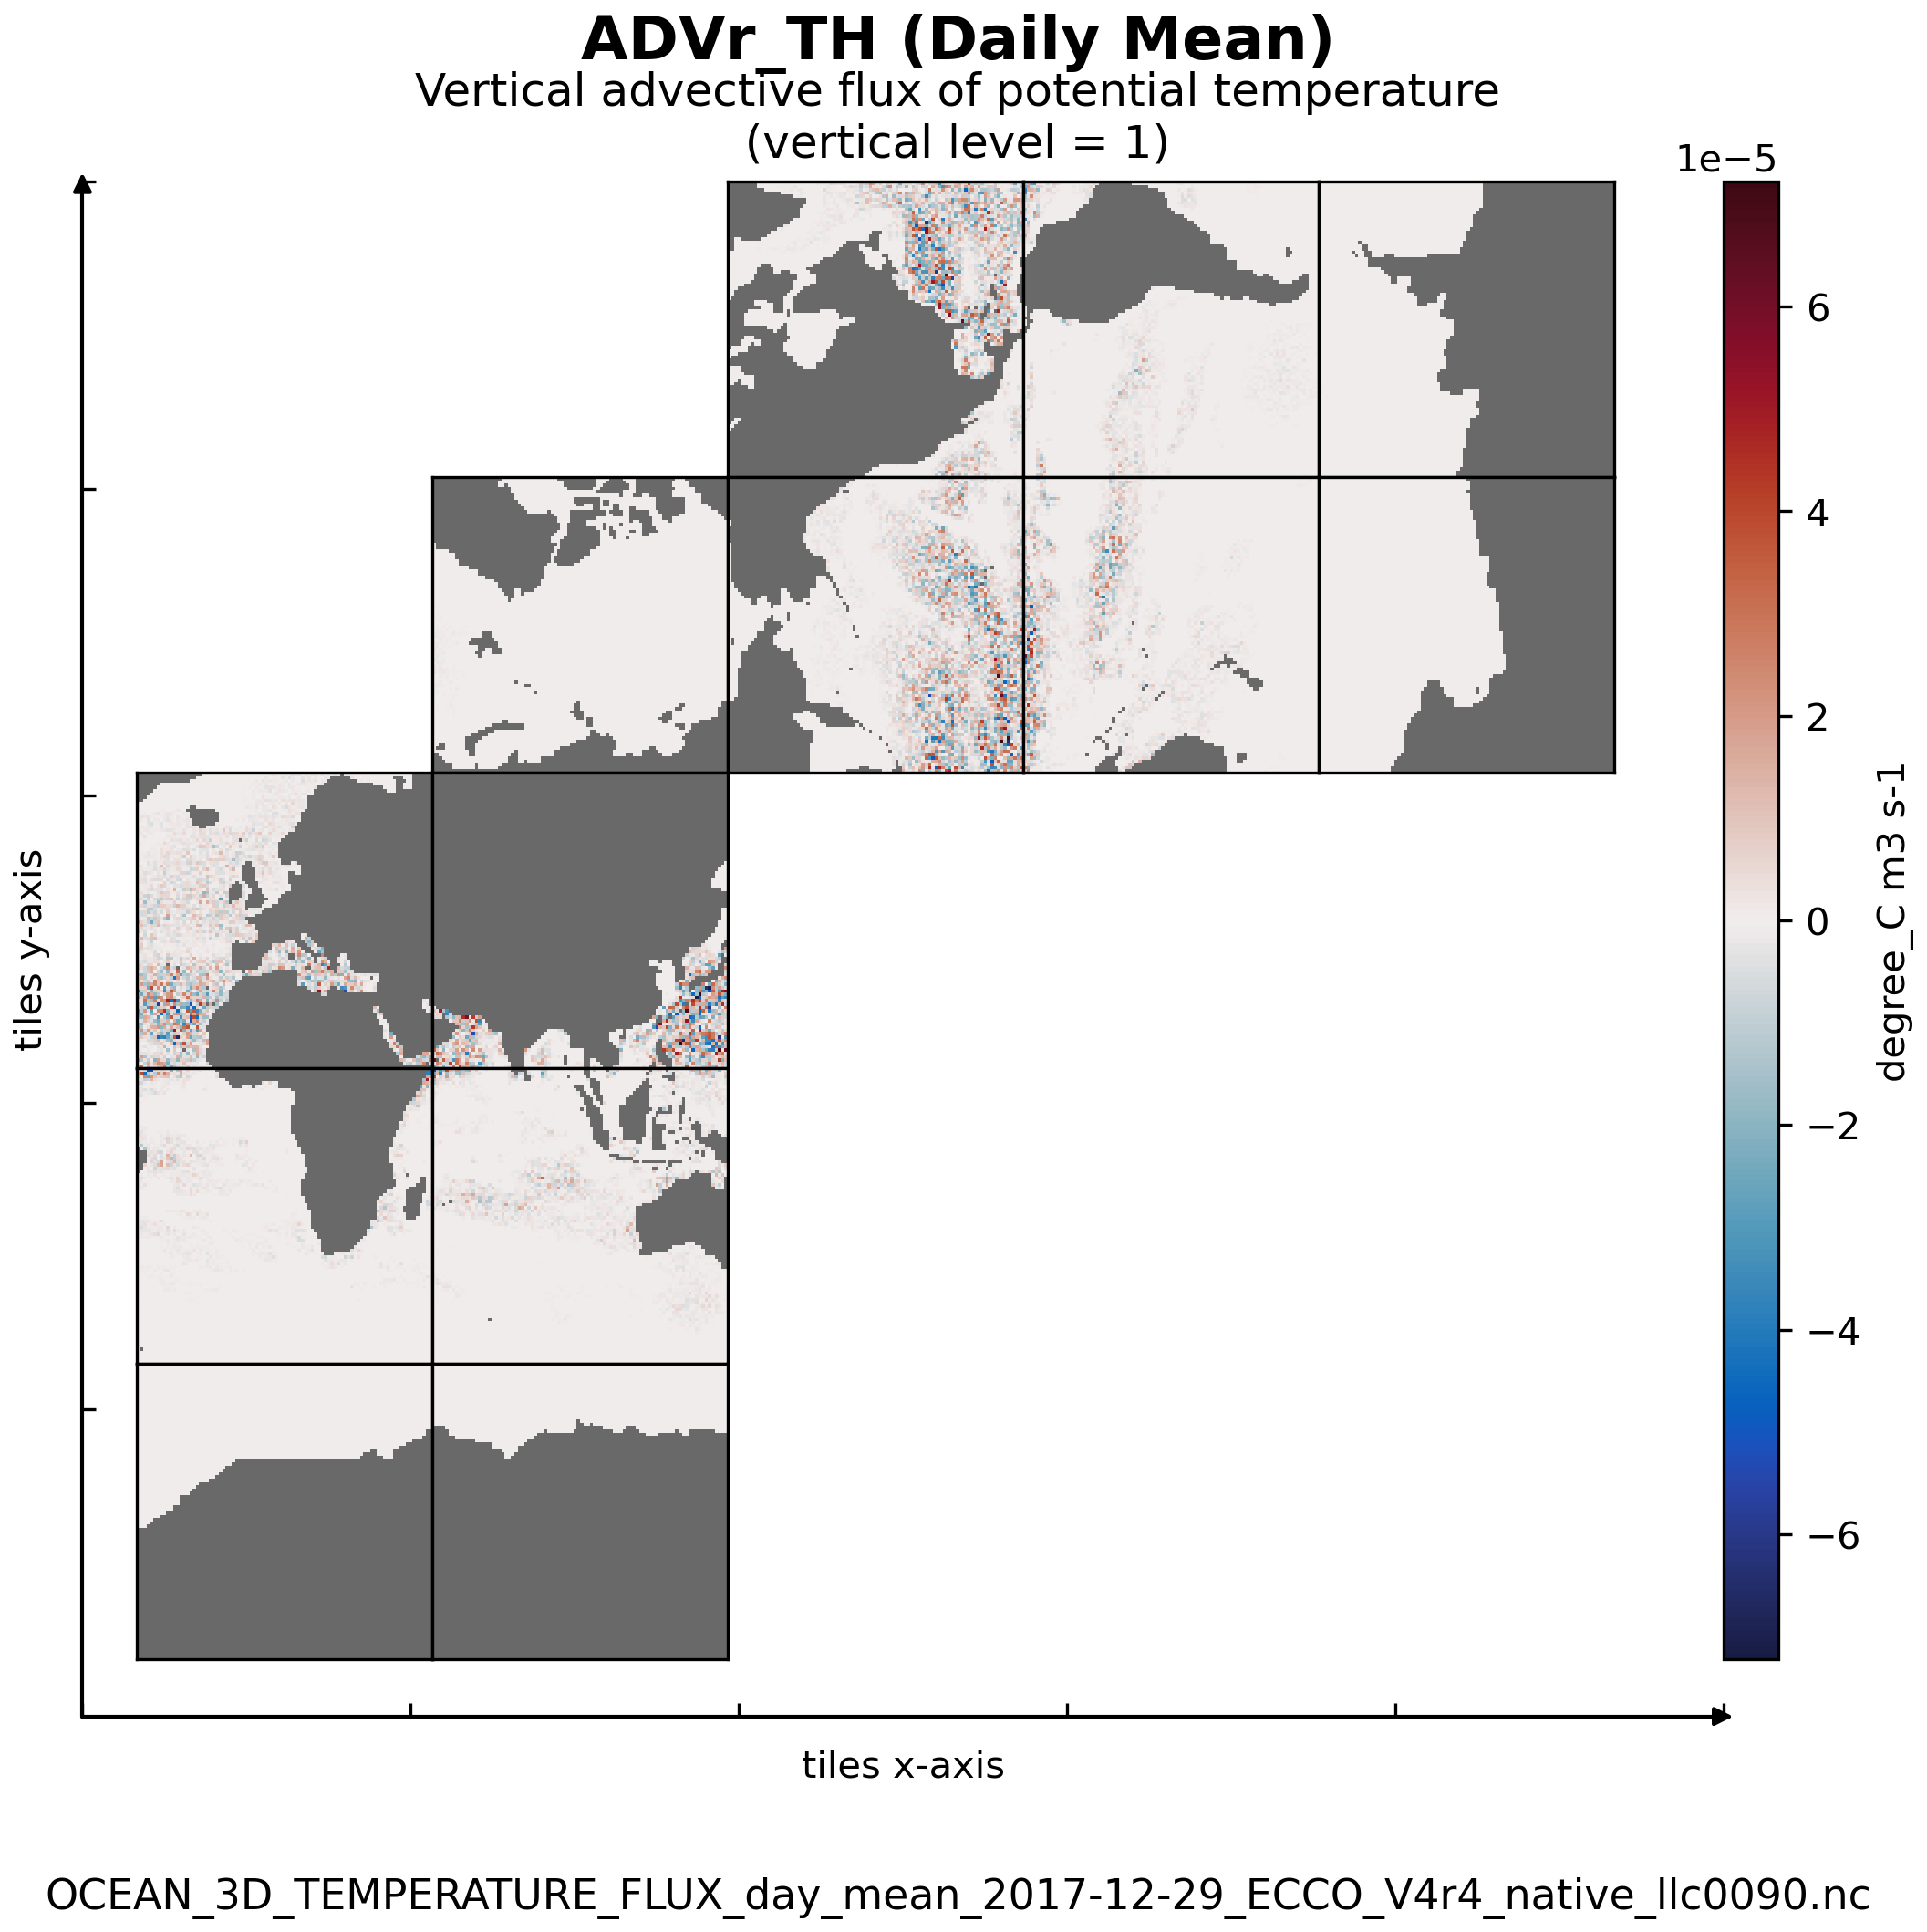
\includegraphics[scale=0.55]{../images/plots/v4r4/native_plots/Ocean_Three-Dimensional_Potential_Temperature_Fluxes/ADVr_TH.png}
\caption{Dataset: OCEAN\_3D\_TEMPERATURE\_FLUX, Variable: ADVr\_TH}
\label{tab:table-OCEAN_3D_TEMPERATURE_FLUX_ADVr_TH-Plot}
\end{figure}
\newpage
\pagebreak
\subsubsection{Native Variable: ADVx\_TH}
\begin{longtable}{|m{0.06\textwidth}|m{0.3\textwidth}|m{0.45\textwidth}|m{0.12\textwidth}|}
\caption{Attributes description of the variable 'ADVx\_TH' from OCEAN\_3D\_TEMPERATURE\_FLUX's  dataset.}
\label{tab:table-OCEAN_3D_TEMPERATURE_FLUX_ADVx_TH} \\ 
\hline \endhead \hline \endfoot
\rowcolor{lightgray} \textbf{Storage Type} & \textbf{Variable Name} & \textbf{Description} & \textbf{Unit} \\ \hline
float32 & ADVx\_TH & Lateral advective flux of potential temperature in the model +x direction & degree\_C m3 s-1 \\ \hline
\multicolumn{4}{|c|}{\cellcolor{lightgray}{\textbf{Description of the variable in Common Data language (CDL)}}} \\ \hline
\multicolumn{4}{|c|}{\fontfamily{lmtt}\selectfont{\makecell{\parbox{.95\textwidth}{\vspace*{0.25cm} \footnotesize{float32 ADVx\_TH(time, k, tile, j, i\_g)\\
\hspace*{0.5cm}ADVx\_TH: \_FillValue = 9.96921e+36\\
\hspace*{0.5cm}ADVx\_TH: coordinates = time Z\\
\hspace*{0.5cm}ADVx\_TH: coverage\_content\_type = modelResult\\
\hspace*{0.5cm}ADVx\_TH: direction = >0 increases potential temperature (THETA)\\
\hspace*{0.5cm}ADVx\_TH: long\_name = Lateral advective flux of potential temperature in the model +x direction\\
\hspace*{0.5cm}ADVx\_TH: mate = ADVy TH\\
\hspace*{0.5cm}ADVx\_TH: units = degree C m3 s-1\\
\hspace*{0.5cm}ADVx\_TH: valid\_max = 38049636.0\\
\hspace*{0.5cm}ADVx\_TH: valid\_min = -38210700.0\\
}}}}} \\ \hline
\rowcolor{lightgray} \multicolumn{4}{|c|}{\textbf{Comments}} \\ \hline
\multicolumn{4}{|p{1\textwidth}|}{\footnotesize{{Lateral advective flux of potential temperature (theta) in the +x direction through the 'u' face of the tracer cell on the native model grid. note: in the arakawa-c grid, horizontal flux quantities are staggered relative to the tracer cells with indexing such that +advx\_th(i\_g,j,k) corresponds to +x fluxes through the 'u' face of the tracer cell at (i,j,k). also, the model +x direction does not necessarily correspond to the geographical east-west direction because the x and y axes of the model's lat-lon-cap (llc) curvilinear lat-lon-cap (llc) grid have arbitrary orientations which vary within and across tiles.}}} \\ \hline
\end{longtable}

\begin{figure}[H]
\centering
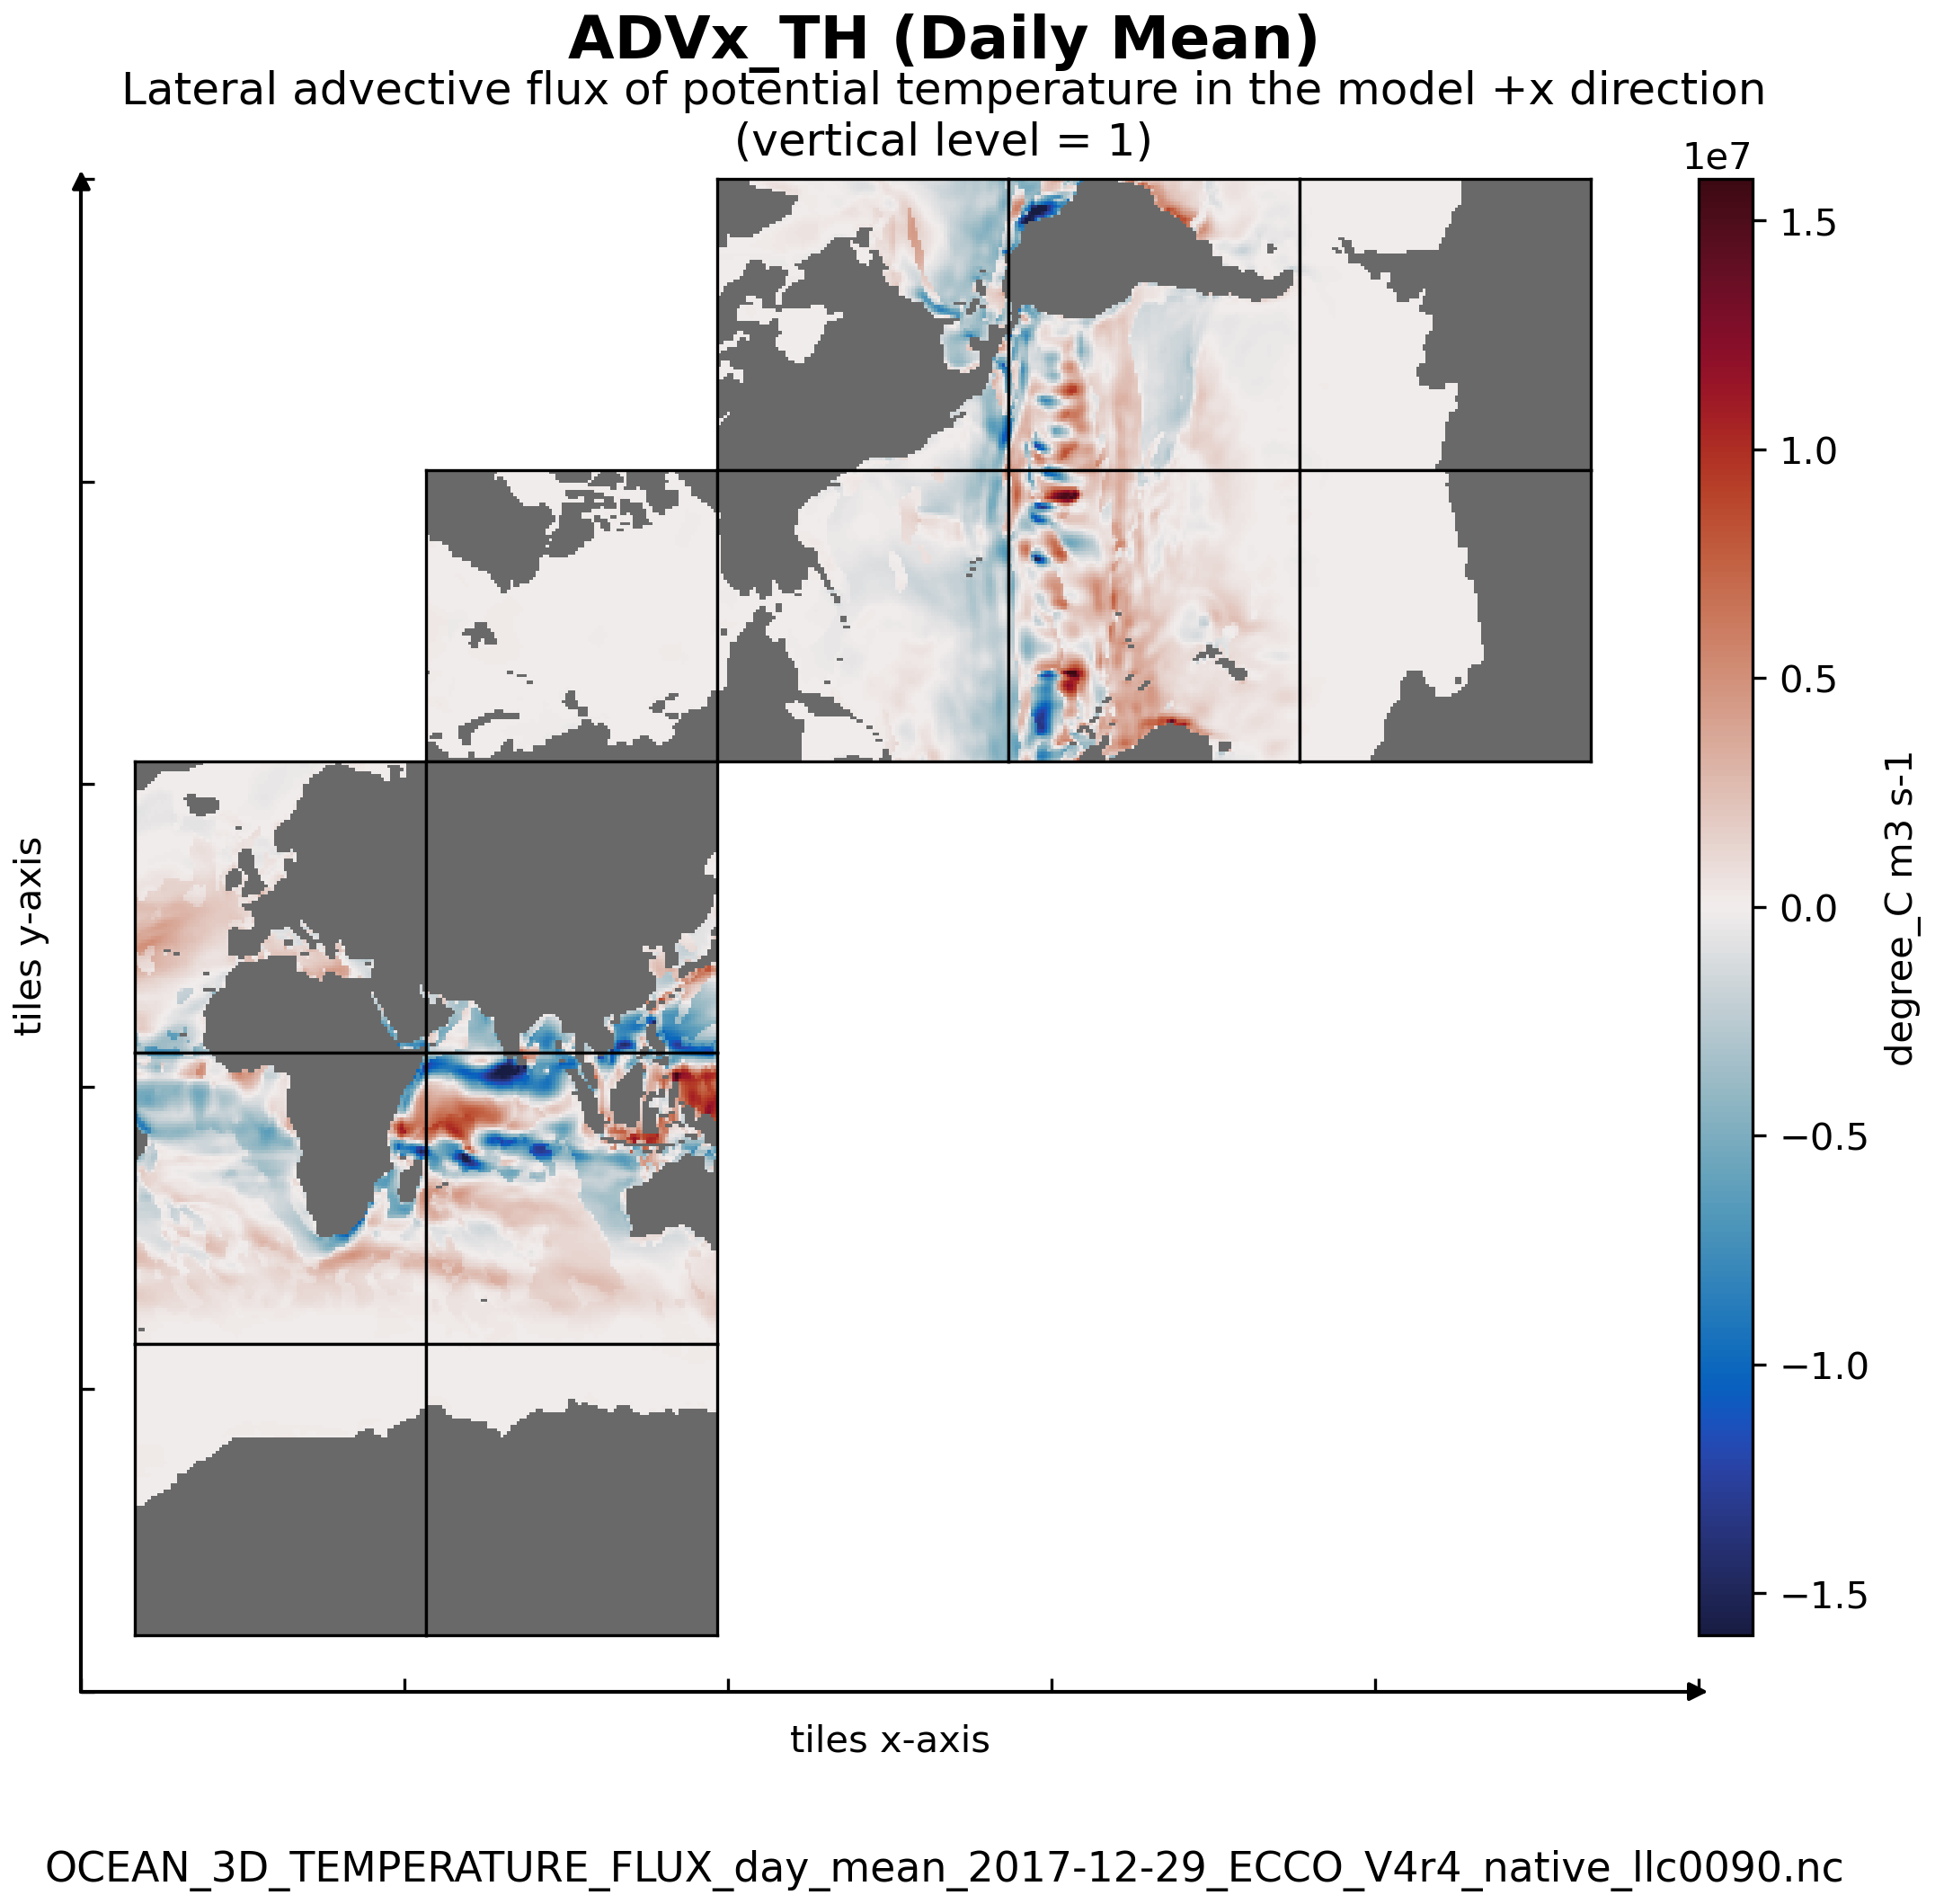
\includegraphics[scale=0.55]{../images/plots/v4r4/native_plots/Ocean_Three-Dimensional_Potential_Temperature_Fluxes/ADVx_TH.png}
\caption{Dataset: OCEAN\_3D\_TEMPERATURE\_FLUX, Variable: ADVx\_TH}
\label{tab:table-OCEAN_3D_TEMPERATURE_FLUX_ADVx_TH-Plot}
\end{figure}
\newpage
\pagebreak
\subsubsection{Native Variable: ADVy\_TH}
\begin{longtable}{|m{0.06\textwidth}|m{0.3\textwidth}|m{0.45\textwidth}|m{0.12\textwidth}|}
\caption{Attributes description of the variable 'ADVy\_TH' from OCEAN\_3D\_TEMPERATURE\_FLUX's  dataset.}
\label{tab:table-OCEAN_3D_TEMPERATURE_FLUX_ADVy_TH} \\ 
\hline \endhead \hline \endfoot
\rowcolor{lightgray} \textbf{Storage Type} & \textbf{Variable Name} & \textbf{Description} & \textbf{Unit} \\ \hline
float32 & ADVy\_TH & Lateral advective flux of potential temperature in the model +y direction & degree\_C m3 s-1 \\ \hline
\multicolumn{4}{|c|}{\cellcolor{lightgray}{\textbf{Description of the variable in Common Data language (CDL)}}} \\ \hline
\multicolumn{4}{|c|}{\fontfamily{lmtt}\selectfont{\makecell{\parbox{.95\textwidth}{\vspace*{0.25cm} \footnotesize{float32 ADVy\_TH(time, k, tile, j\_g, i)\\
\hspace*{0.5cm}ADVy\_TH: \_FillValue = 9.96921e+36\\
\hspace*{0.5cm}ADVy\_TH: coordinates = time Z\\
\hspace*{0.5cm}ADVy\_TH: coverage\_content\_type = modelResult\\
\hspace*{0.5cm}ADVy\_TH: direction = >0 increases potential temperature (THETA)\\
\hspace*{0.5cm}ADVy\_TH: long\_name = Lateral advective flux of potential temperature in the model +y direction\\
\hspace*{0.5cm}ADVy\_TH: mate = ADVx TH\\
\hspace*{0.5cm}ADVy\_TH: units = degree C m3 s-1\\
\hspace*{0.5cm}ADVy\_TH: valid\_max = 56347884.0\\
\hspace*{0.5cm}ADVy\_TH: valid\_min = -43909120.0\\
}}}}} \\ \hline
\rowcolor{lightgray} \multicolumn{4}{|c|}{\textbf{Comments}} \\ \hline
\multicolumn{4}{|p{1\textwidth}|}{\footnotesize{{Lateral advective flux of potential temperature (theta) in the +y direction through the 'v' face of the tracer cell on the native model grid. note: in the arakawa-c grid, horizontal flux quantities are staggered relative to the tracer cells with indexing such that +advy\_th(i,j\_g,k) corresponds to +y fluxes through the 'v' face of the tracer cell at (i,j,k). also, the model +y direction does not necessarily correspond to the geographical north-south direction because the x and y axes of the model's curvilinear lat-lon-cap (llc) grid have arbitrary orientations which vary within and across tiles.}}} \\ \hline
\end{longtable}

\begin{figure}[H]
\centering
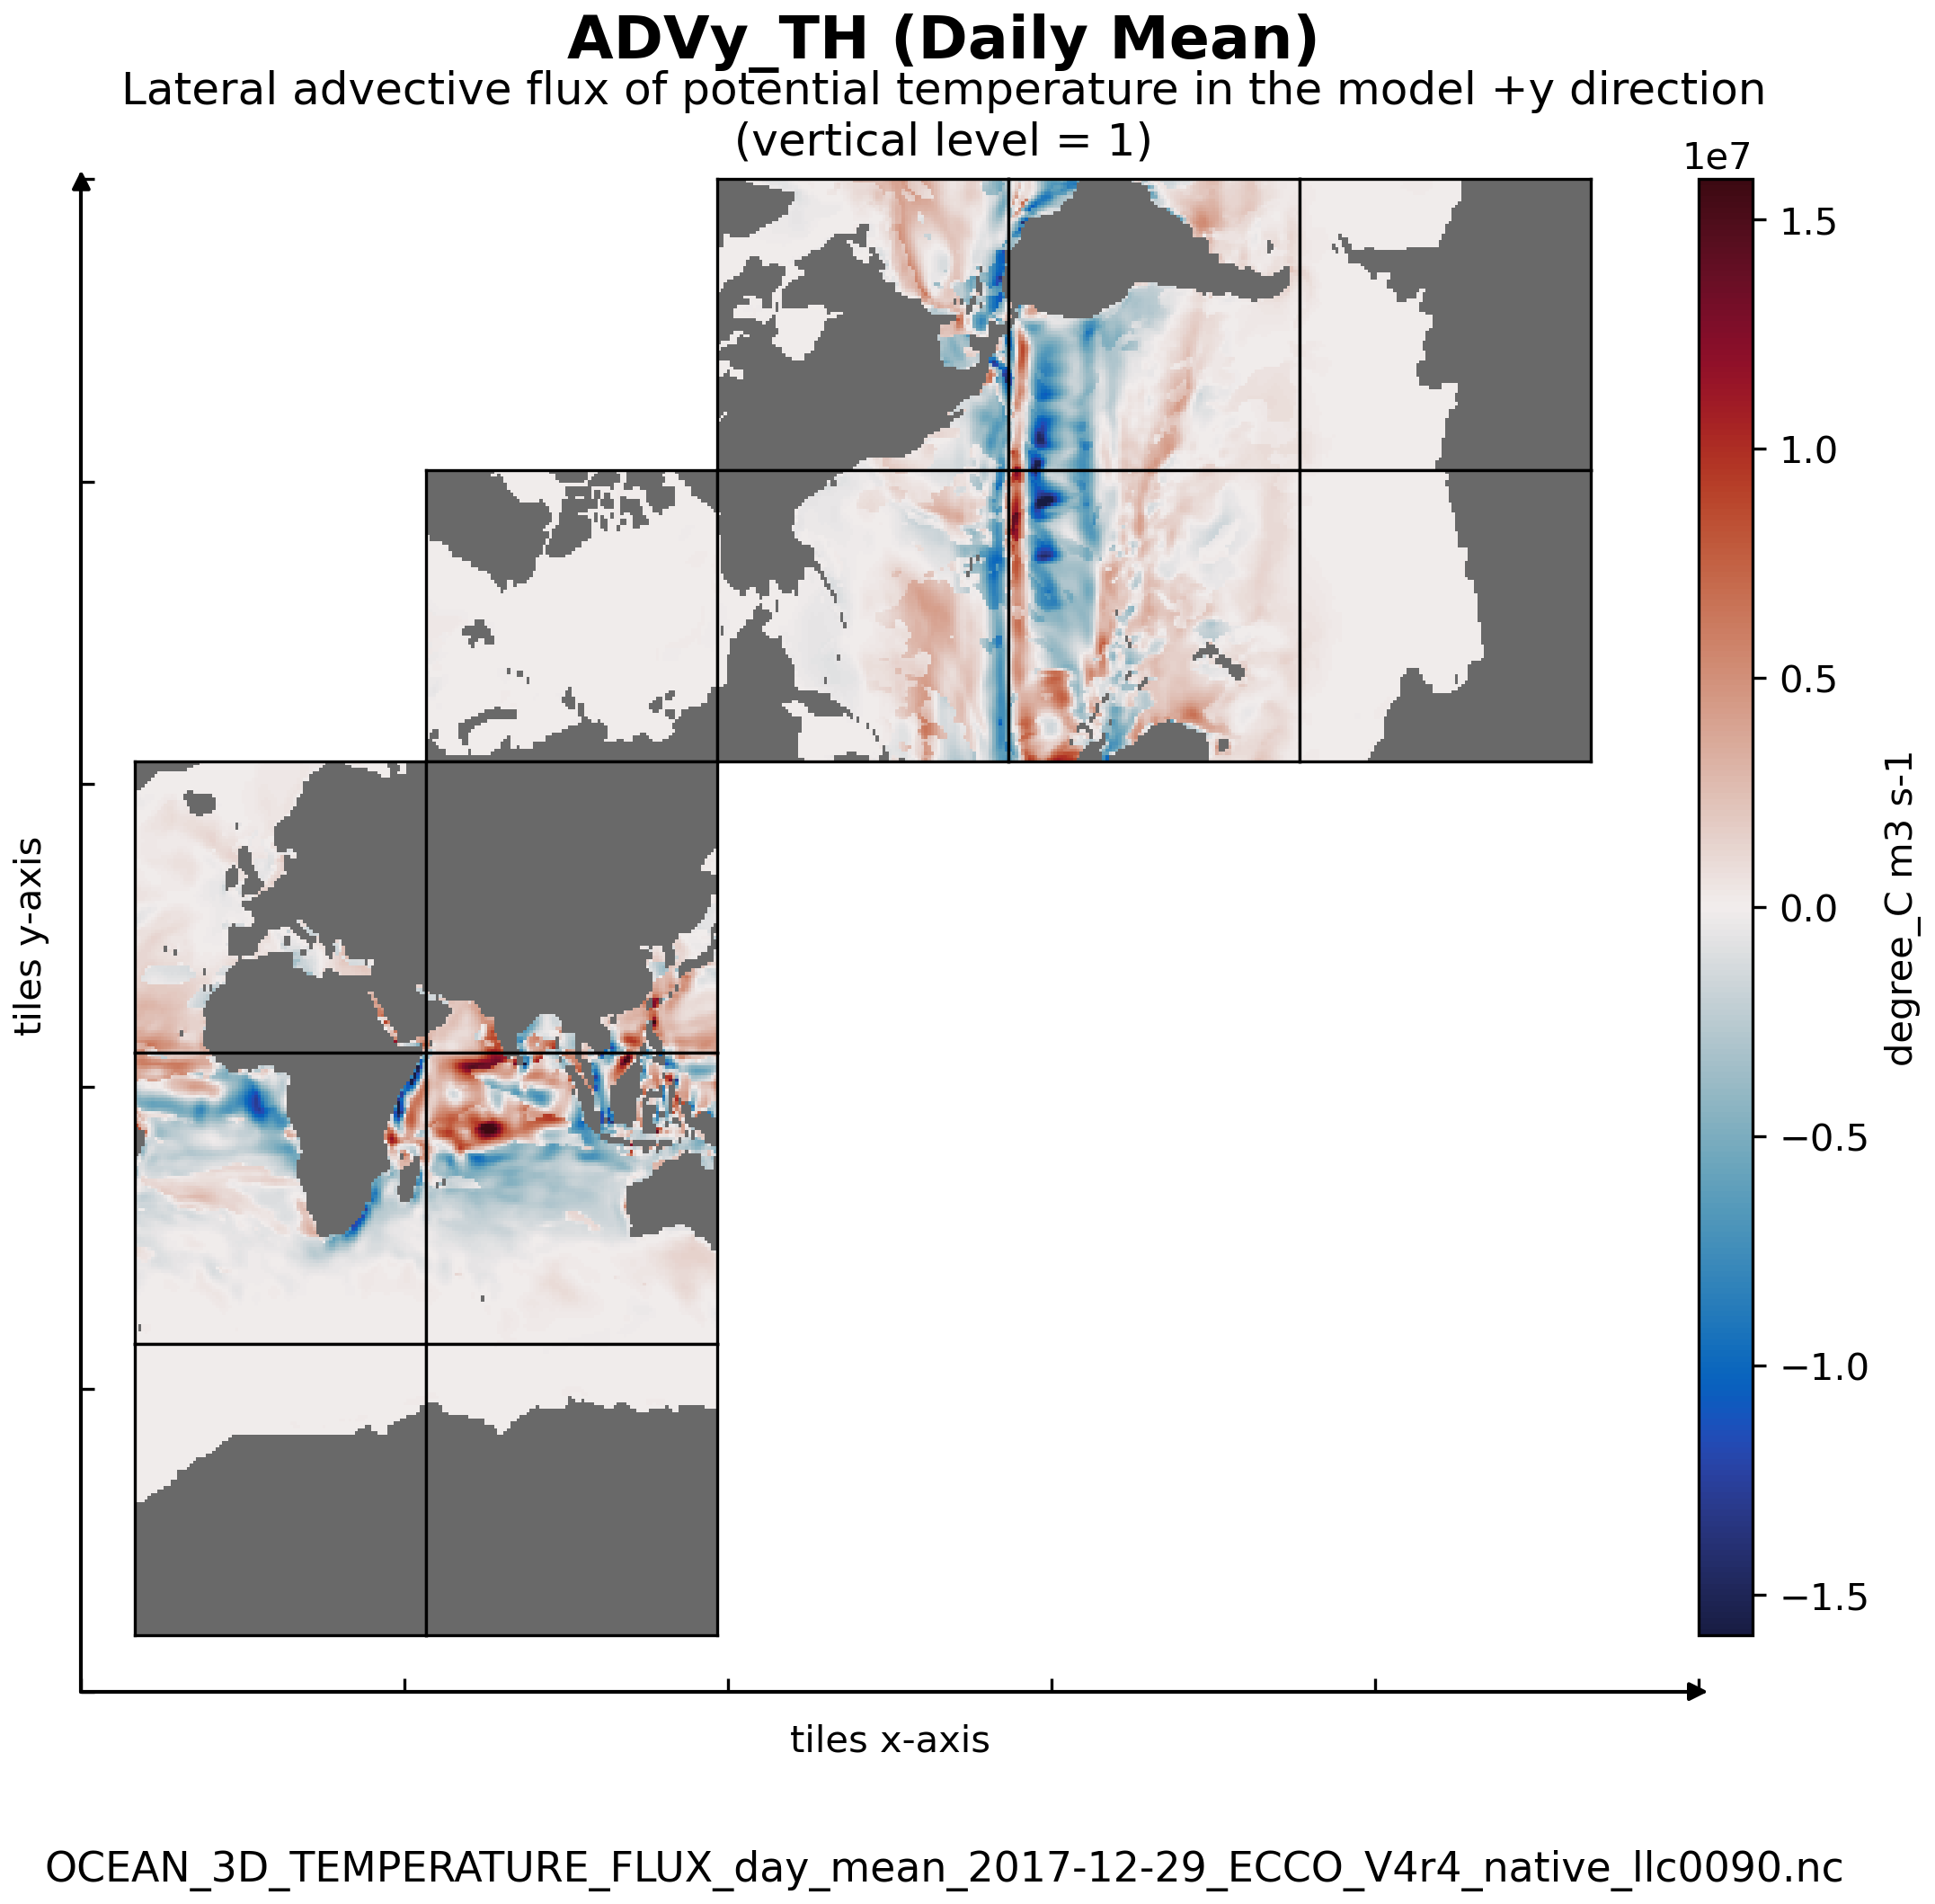
\includegraphics[scale=0.55]{../images/plots/v4r4/native_plots/Ocean_Three-Dimensional_Potential_Temperature_Fluxes/ADVy_TH.png}
\caption{Dataset: OCEAN\_3D\_TEMPERATURE\_FLUX, Variable: ADVy\_TH}
\label{tab:table-OCEAN_3D_TEMPERATURE_FLUX_ADVy_TH-Plot}
\end{figure}
\newpage
\pagebreak
\subsubsection{Native Variable: DFrE\_TH}
\begin{longtable}{|m{0.06\textwidth}|m{0.3\textwidth}|m{0.45\textwidth}|m{0.12\textwidth}|}
\caption{Attributes description of the variable 'DFrE\_TH' from OCEAN\_3D\_TEMPERATURE\_FLUX's  dataset.}
\label{tab:table-OCEAN_3D_TEMPERATURE_FLUX_DFrE_TH} \\ 
\hline \endhead \hline \endfoot
\rowcolor{lightgray} \textbf{Storage Type} & \textbf{Variable Name} & \textbf{Description} & \textbf{Unit} \\ \hline
float32 & DFrE\_TH & Vertical diffusive flux of potential temperature (explicit term) & degree\_C m3 s-1 \\ \hline
\multicolumn{4}{|c|}{\cellcolor{lightgray}{\textbf{Description of the variable in Common Data language (CDL)}}} \\ \hline
\multicolumn{4}{|c|}{\fontfamily{lmtt}\selectfont{\makecell{\parbox{.95\textwidth}{\vspace*{0.25cm} \footnotesize{float32 DFrE\_TH(time, k\_l, tile, j, i)\\
\hspace*{0.5cm}DFrE\_TH: \_FillValue = 9.96921e+36\\
\hspace*{0.5cm}DFrE\_TH: coordinates = XC YC time Zl\\
\hspace*{0.5cm}DFrE\_TH: coverage\_content\_type = modelResult\\
\hspace*{0.5cm}DFrE\_TH: direction = >0 decreases potential temperature (THETA)\\
\hspace*{0.5cm}DFrE\_TH: long\_name = Vertical diffusive flux of potential temperature (explicit term)\\
\hspace*{0.5cm}DFrE\_TH: units = degree C m3 s-1\\
\hspace*{0.5cm}DFrE\_TH: valid\_max = 2659875.25\\
\hspace*{0.5cm}DFrE\_TH: valid\_min = -2632379.75\\
}}}}} \\ \hline
\rowcolor{lightgray} \multicolumn{4}{|c|}{\textbf{Comments}} \\ \hline
\multicolumn{4}{|p{1\textwidth}|}{\footnotesize{{The explicit term of the vertical diffusive flux of potential temperature (theta) in the +z direction through the top 'w' face of the tracer cell on the native model grid. in the ecco v4r4 model, an implicit scheme is used to calculate vertical diffusive tracer fluxes due to background diffusivity and the kwz component of the gm-redi tensor (vertical flux as a function of vertical gradient) while an explicit scheme is used to calculate the vertical diffusive fluxes from the kwx and kwy components of the gm-redi tensor (vertical flux as a function of horizontal gradient). both implicit and explicit components of vertical diffusive flux of potential temperature are provided. note: in the arakawa-c grid, vertical flux quantities are staggered relative to the tracer cells with indexing such that +dfre\_th(i,j,k\_l) corresponds to upward +z fluxes through the top 'w' face of the tracer cell at (i,j,k).}}} \\ \hline
\end{longtable}

\begin{figure}[H]
\centering
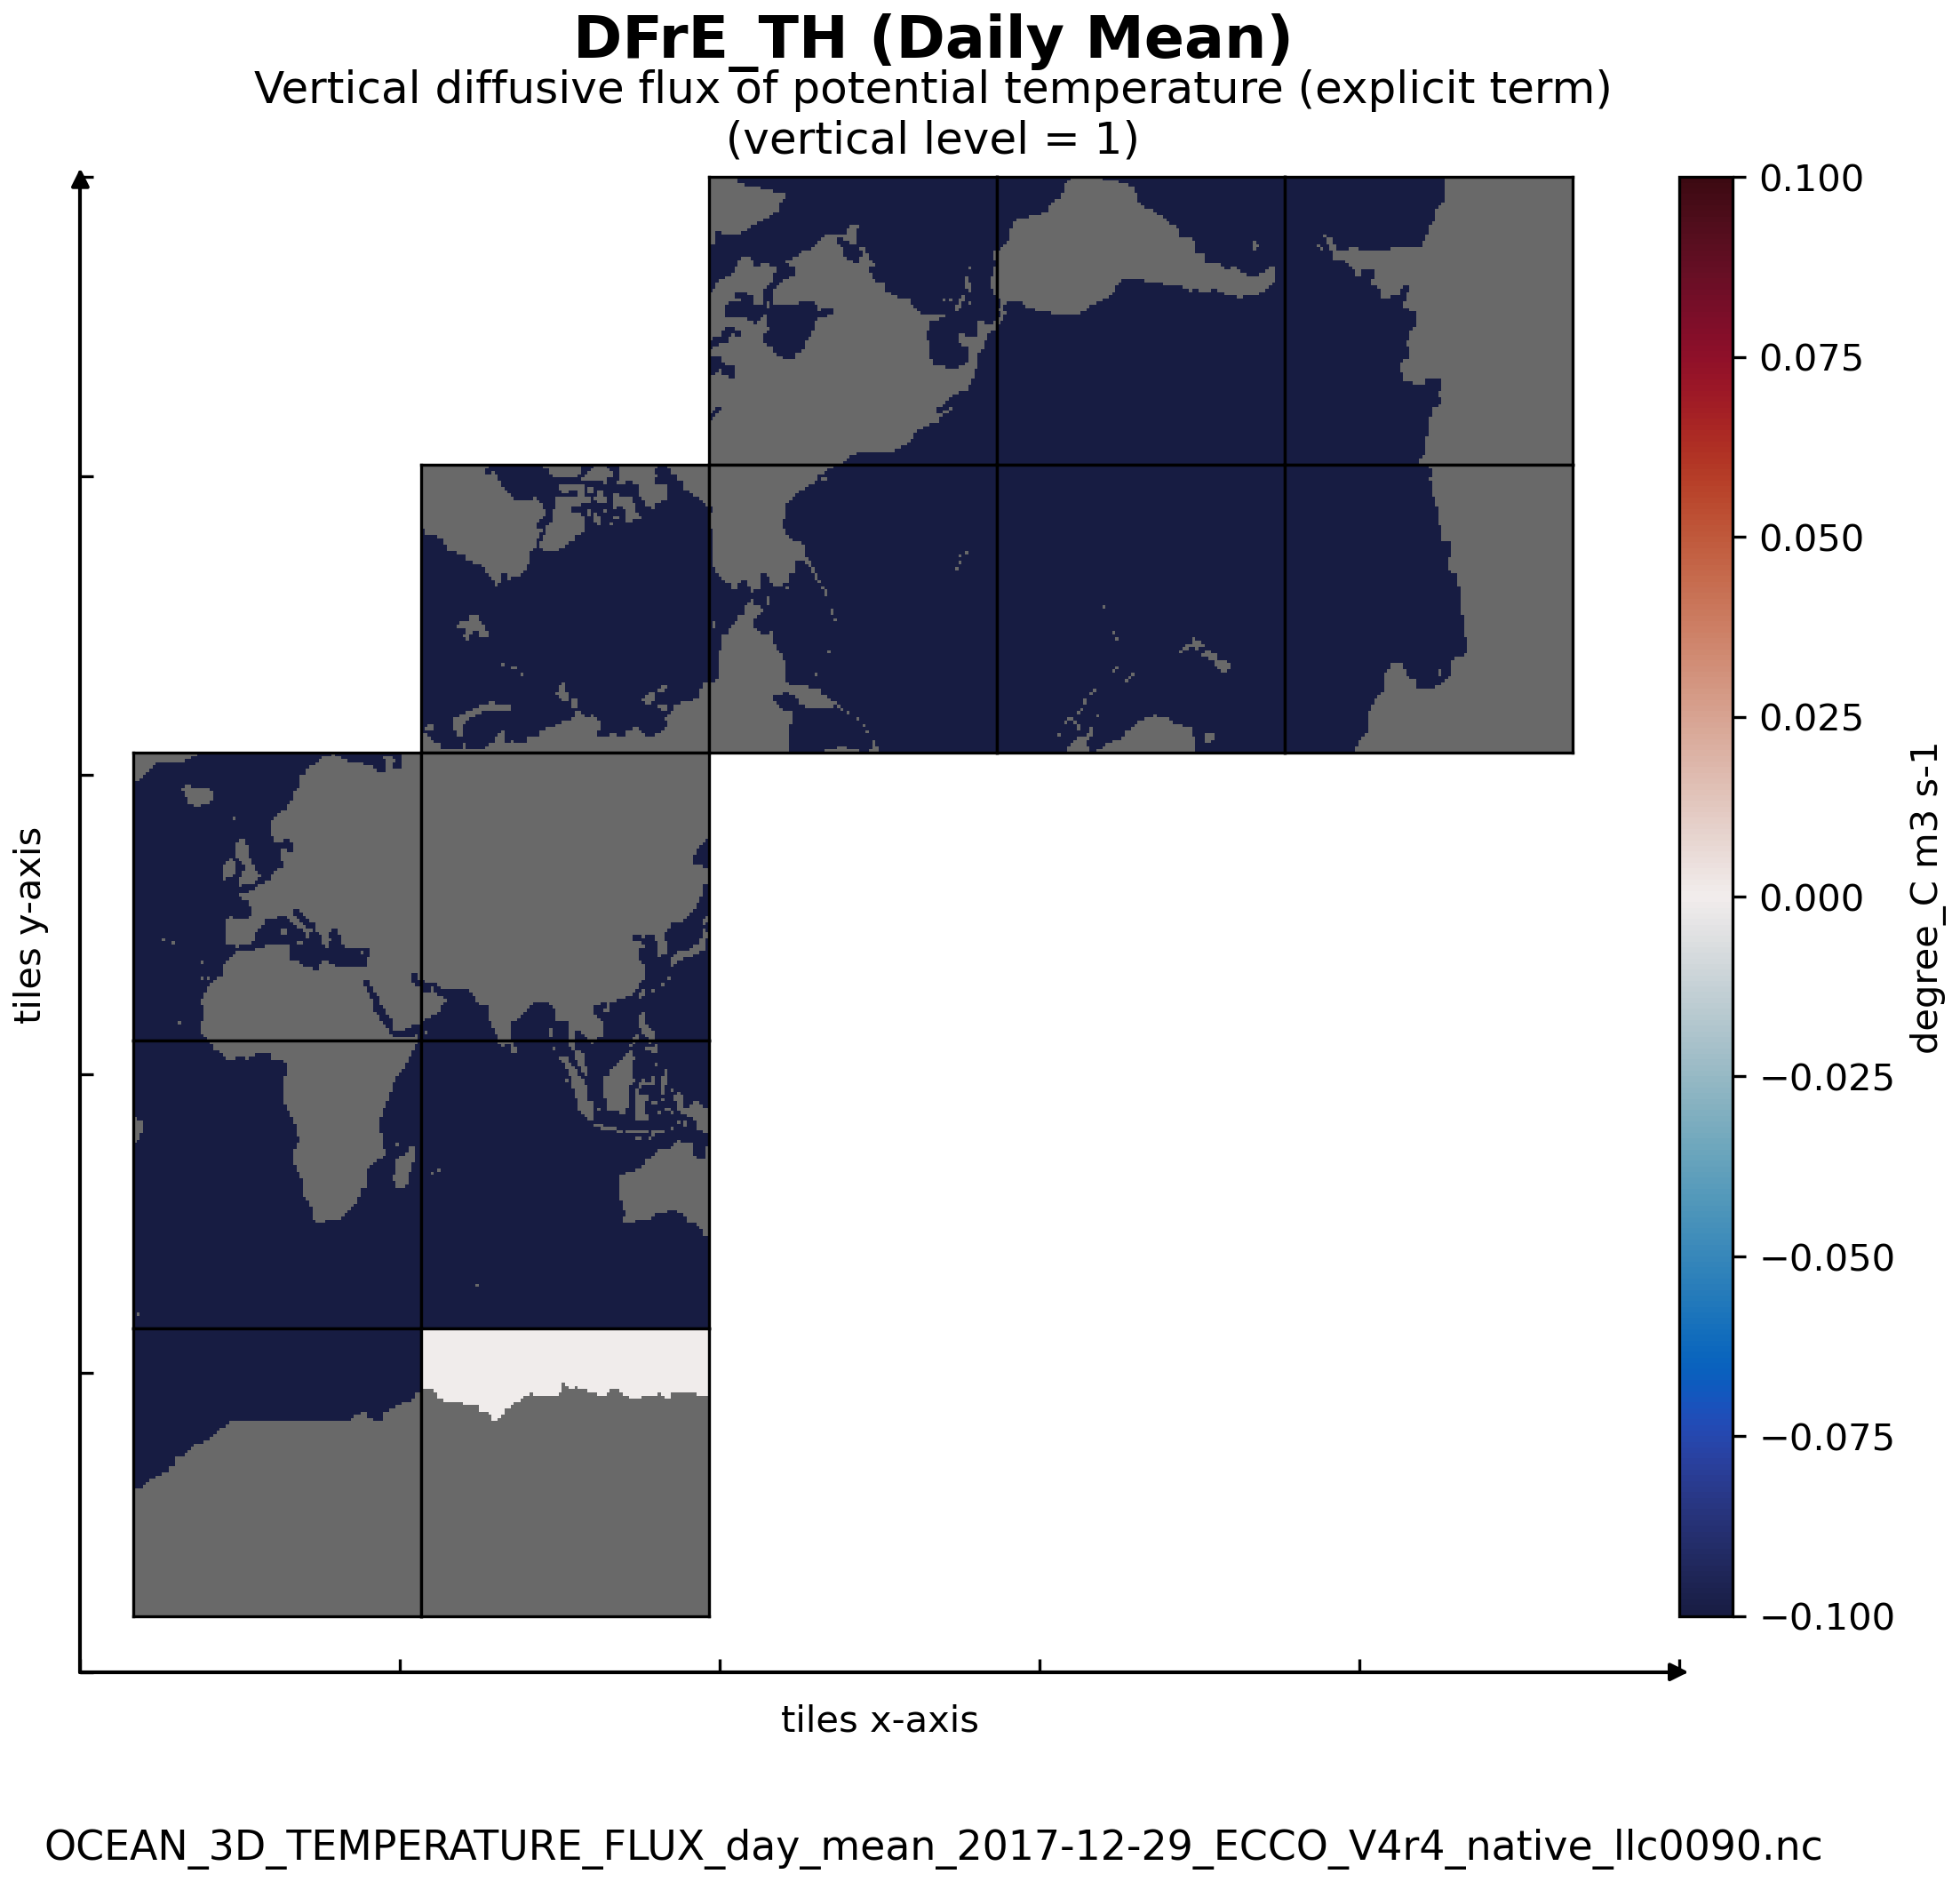
\includegraphics[scale=0.55]{../images/plots/v4r4/native_plots/Ocean_Three-Dimensional_Potential_Temperature_Fluxes/DFrE_TH.png}
\caption{Dataset: OCEAN\_3D\_TEMPERATURE\_FLUX, Variable: DFrE\_TH}
\label{tab:table-OCEAN_3D_TEMPERATURE_FLUX_DFrE_TH-Plot}
\end{figure}
\newpage
\pagebreak
\subsubsection{Native Variable: DFrI\_TH}
\begin{longtable}{|m{0.06\textwidth}|m{0.3\textwidth}|m{0.45\textwidth}|m{0.12\textwidth}|}
\caption{Attributes description of the variable 'DFrI\_TH' from OCEAN\_3D\_TEMPERATURE\_FLUX's  dataset.}
\label{tab:table-OCEAN_3D_TEMPERATURE_FLUX_DFrI_TH} \\ 
\hline \endhead \hline \endfoot
\rowcolor{lightgray} \textbf{Storage Type} & \textbf{Variable Name} & \textbf{Description} & \textbf{Unit} \\ \hline
float32 & DFrI\_TH & Vertical diffusive flux of potential temperature (implicit term) & degree\_C m3 s-1 \\ \hline
\multicolumn{4}{|c|}{\cellcolor{lightgray}{\textbf{Description of the variable in Common Data language (CDL)}}} \\ \hline
\multicolumn{4}{|c|}{\fontfamily{lmtt}\selectfont{\makecell{\parbox{.95\textwidth}{\vspace*{0.25cm} \footnotesize{float32 DFrI\_TH(time, k\_l, tile, j, i)\\
\hspace*{0.5cm}DFrI\_TH: \_FillValue = 9.96921e+36\\
\hspace*{0.5cm}DFrI\_TH: coordinates = XC YC time Zl\\
\hspace*{0.5cm}DFrI\_TH: coverage\_content\_type = modelResult\\
\hspace*{0.5cm}DFrI\_TH: direction = >0 decreases potential temperature (THETA)\\
\hspace*{0.5cm}DFrI\_TH: long\_name = Vertical diffusive flux of potential temperature (implicit term)\\
\hspace*{0.5cm}DFrI\_TH: units = degree C m3 s-1\\
\hspace*{0.5cm}DFrI\_TH: valid\_max = 23574302.0\\
\hspace*{0.5cm}DFrI\_TH: valid\_min = -104210688.0\\
}}}}} \\ \hline
\rowcolor{lightgray} \multicolumn{4}{|c|}{\textbf{Comments}} \\ \hline
\multicolumn{4}{|p{1\textwidth}|}{\footnotesize{{The implicit term of the vertical diffusive flux of potential temperature (theta) in the +z direction through the top 'w' face of the tracer cell on the native model grid. in the ecco v4r4 model, an implicit scheme is used to calculate vertical diffusive tracer fluxes due to background diffusivity and the kwz component of the gm-redi tensor (vertical flux as a function of vertical gradient) while an explicit scheme is used to calculate the vertical diffusive fluxes from the kwx and kwy components of the gm-redi tensor (vertical flux as a function of horizontal gradient). both implicit and explicit components of vertical diffusive flux of potential temperature are provided. note: in the arakawa-c grid, vertical flux quantities are staggered relative to the tracer cells with indexing such that +dfri\_th(i,j,k\_l) corresponds to upward +z fluxes through the top 'w' face of the tracer cell at (i,j,k)}}} \\ \hline
\end{longtable}

\begin{figure}[H]
\centering
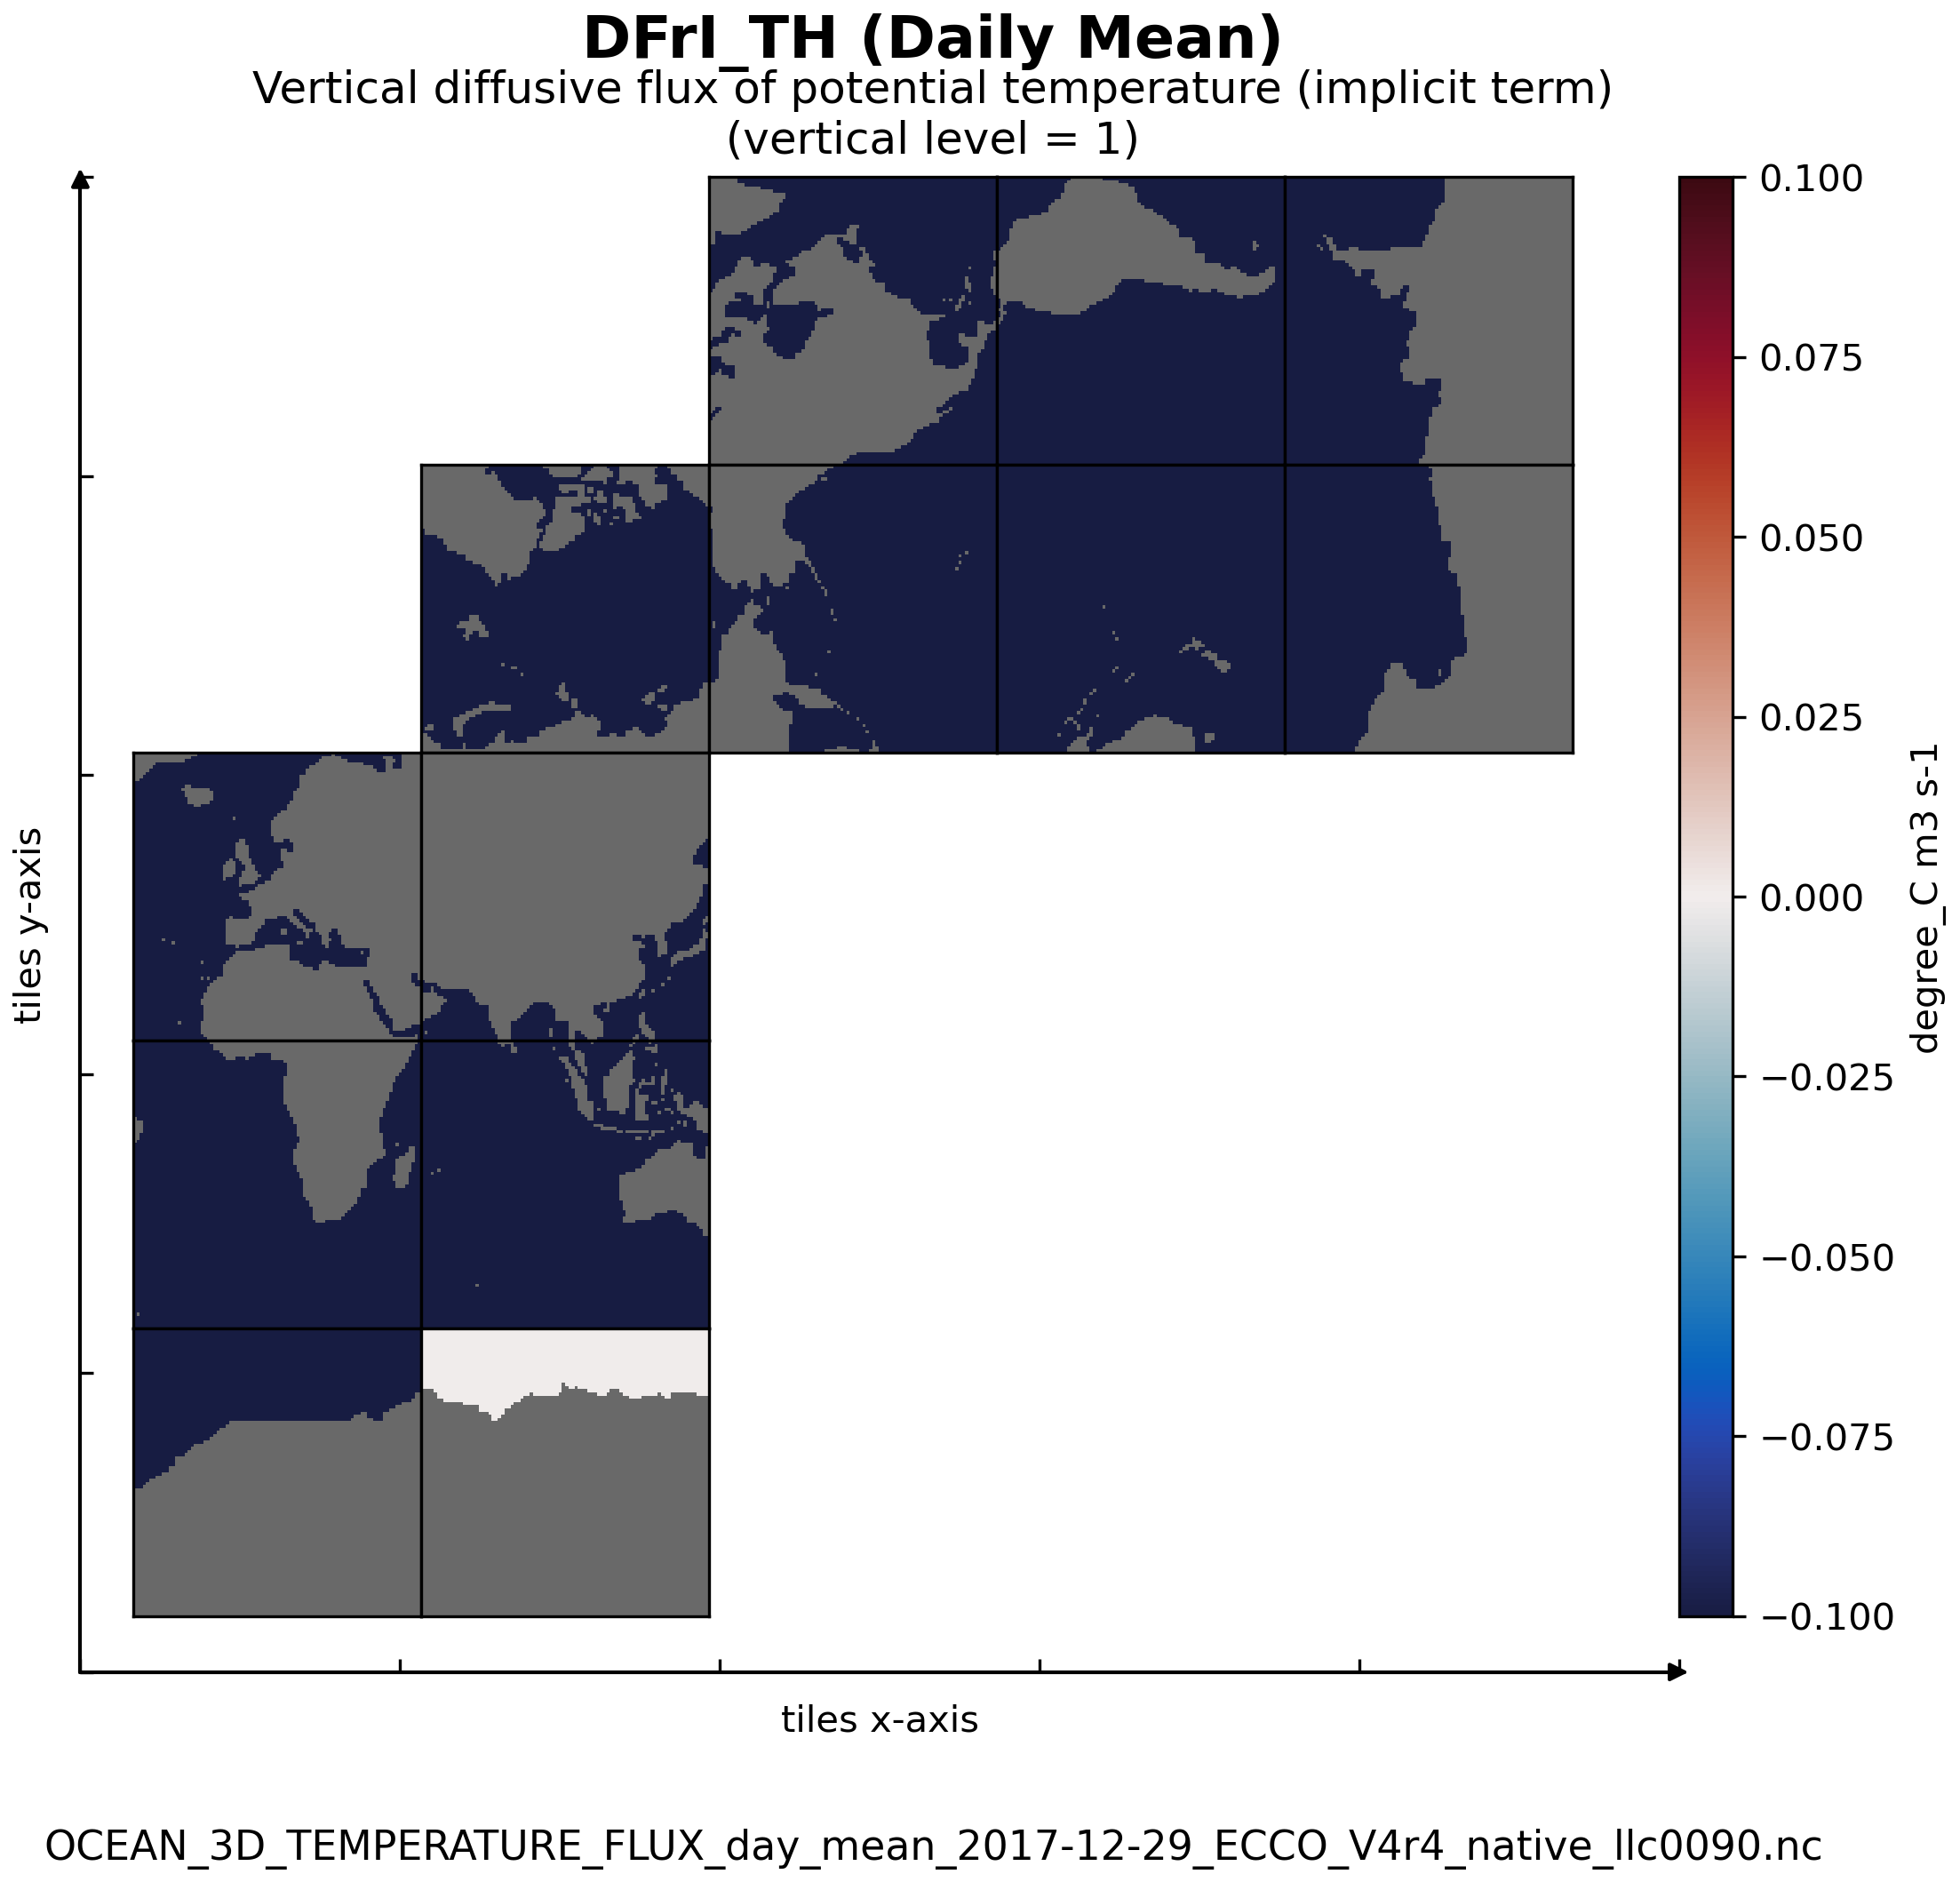
\includegraphics[scale=0.55]{../images/plots/v4r4/native_plots/Ocean_Three-Dimensional_Potential_Temperature_Fluxes/DFrI_TH.png}
\caption{Dataset: OCEAN\_3D\_TEMPERATURE\_FLUX, Variable: DFrI\_TH}
\label{tab:table-OCEAN_3D_TEMPERATURE_FLUX_DFrI_TH-Plot}
\end{figure}
\newpage
\pagebreak
\subsubsection{Native Variable: DFxE\_TH}
\begin{longtable}{|m{0.06\textwidth}|m{0.3\textwidth}|m{0.45\textwidth}|m{0.12\textwidth}|}
\caption{Attributes description of the variable 'DFxE\_TH' from OCEAN\_3D\_TEMPERATURE\_FLUX's  dataset.}
\label{tab:table-OCEAN_3D_TEMPERATURE_FLUX_DFxE_TH} \\ 
\hline \endhead \hline \endfoot
\rowcolor{lightgray} \textbf{Storage Type} & \textbf{Variable Name} & \textbf{Description} & \textbf{Unit} \\ \hline
float32 & DFxE\_TH & Lateral diffusive flux of potential temperature in the model +x direction & degree\_C m3 s-1 \\ \hline
\multicolumn{4}{|c|}{\cellcolor{lightgray}{\textbf{Description of the variable in Common Data language (CDL)}}} \\ \hline
\multicolumn{4}{|c|}{\fontfamily{lmtt}\selectfont{\makecell{\parbox{.95\textwidth}{\vspace*{0.25cm} \footnotesize{float32 DFxE\_TH(time, k, tile, j, i\_g)\\
\hspace*{0.5cm}DFxE\_TH: \_FillValue = 9.96921e+36\\
\hspace*{0.5cm}DFxE\_TH: coordinates = time Z\\
\hspace*{0.5cm}DFxE\_TH: coverage\_content\_type = modelResult\\
\hspace*{0.5cm}DFxE\_TH: direction = >0 increases potential temperature (THETA)\\
\hspace*{0.5cm}DFxE\_TH: long\_name = Lateral diffusive flux of potential temperature in the model +x direction\\
\hspace*{0.5cm}DFxE\_TH: mate = DFyE TH\\
\hspace*{0.5cm}DFxE\_TH: units = degree C m3 s-1\\
\hspace*{0.5cm}DFxE\_TH: valid\_max = 698695.75\\
\hspace*{0.5cm}DFxE\_TH: valid\_min = -582494.125\\
}}}}} \\ \hline
\rowcolor{lightgray} \multicolumn{4}{|c|}{\textbf{Comments}} \\ \hline
\multicolumn{4}{|p{1\textwidth}|}{\footnotesize{{Lateral diffusive flux of potential temperature (theta) in the +x direction through the 'u' face of the tracer cell on the native model grid. note: in the arakawa-c grid, horizontal flux quantities are staggered relative to the tracer cells with indexing such that +dfxe\_th(i\_g,j,k) corresponds to +x fluxes through the 'u' face of the tracer cell at (i,j,k). also, the model +x direction does not necessarily correspond to the geographical east-west direction because the x and y axes of the model's curvilinear lat-lon-cap (llc) grid have arbitrary orientations which vary within and across tiles.}}} \\ \hline
\end{longtable}

\begin{figure}[H]
\centering
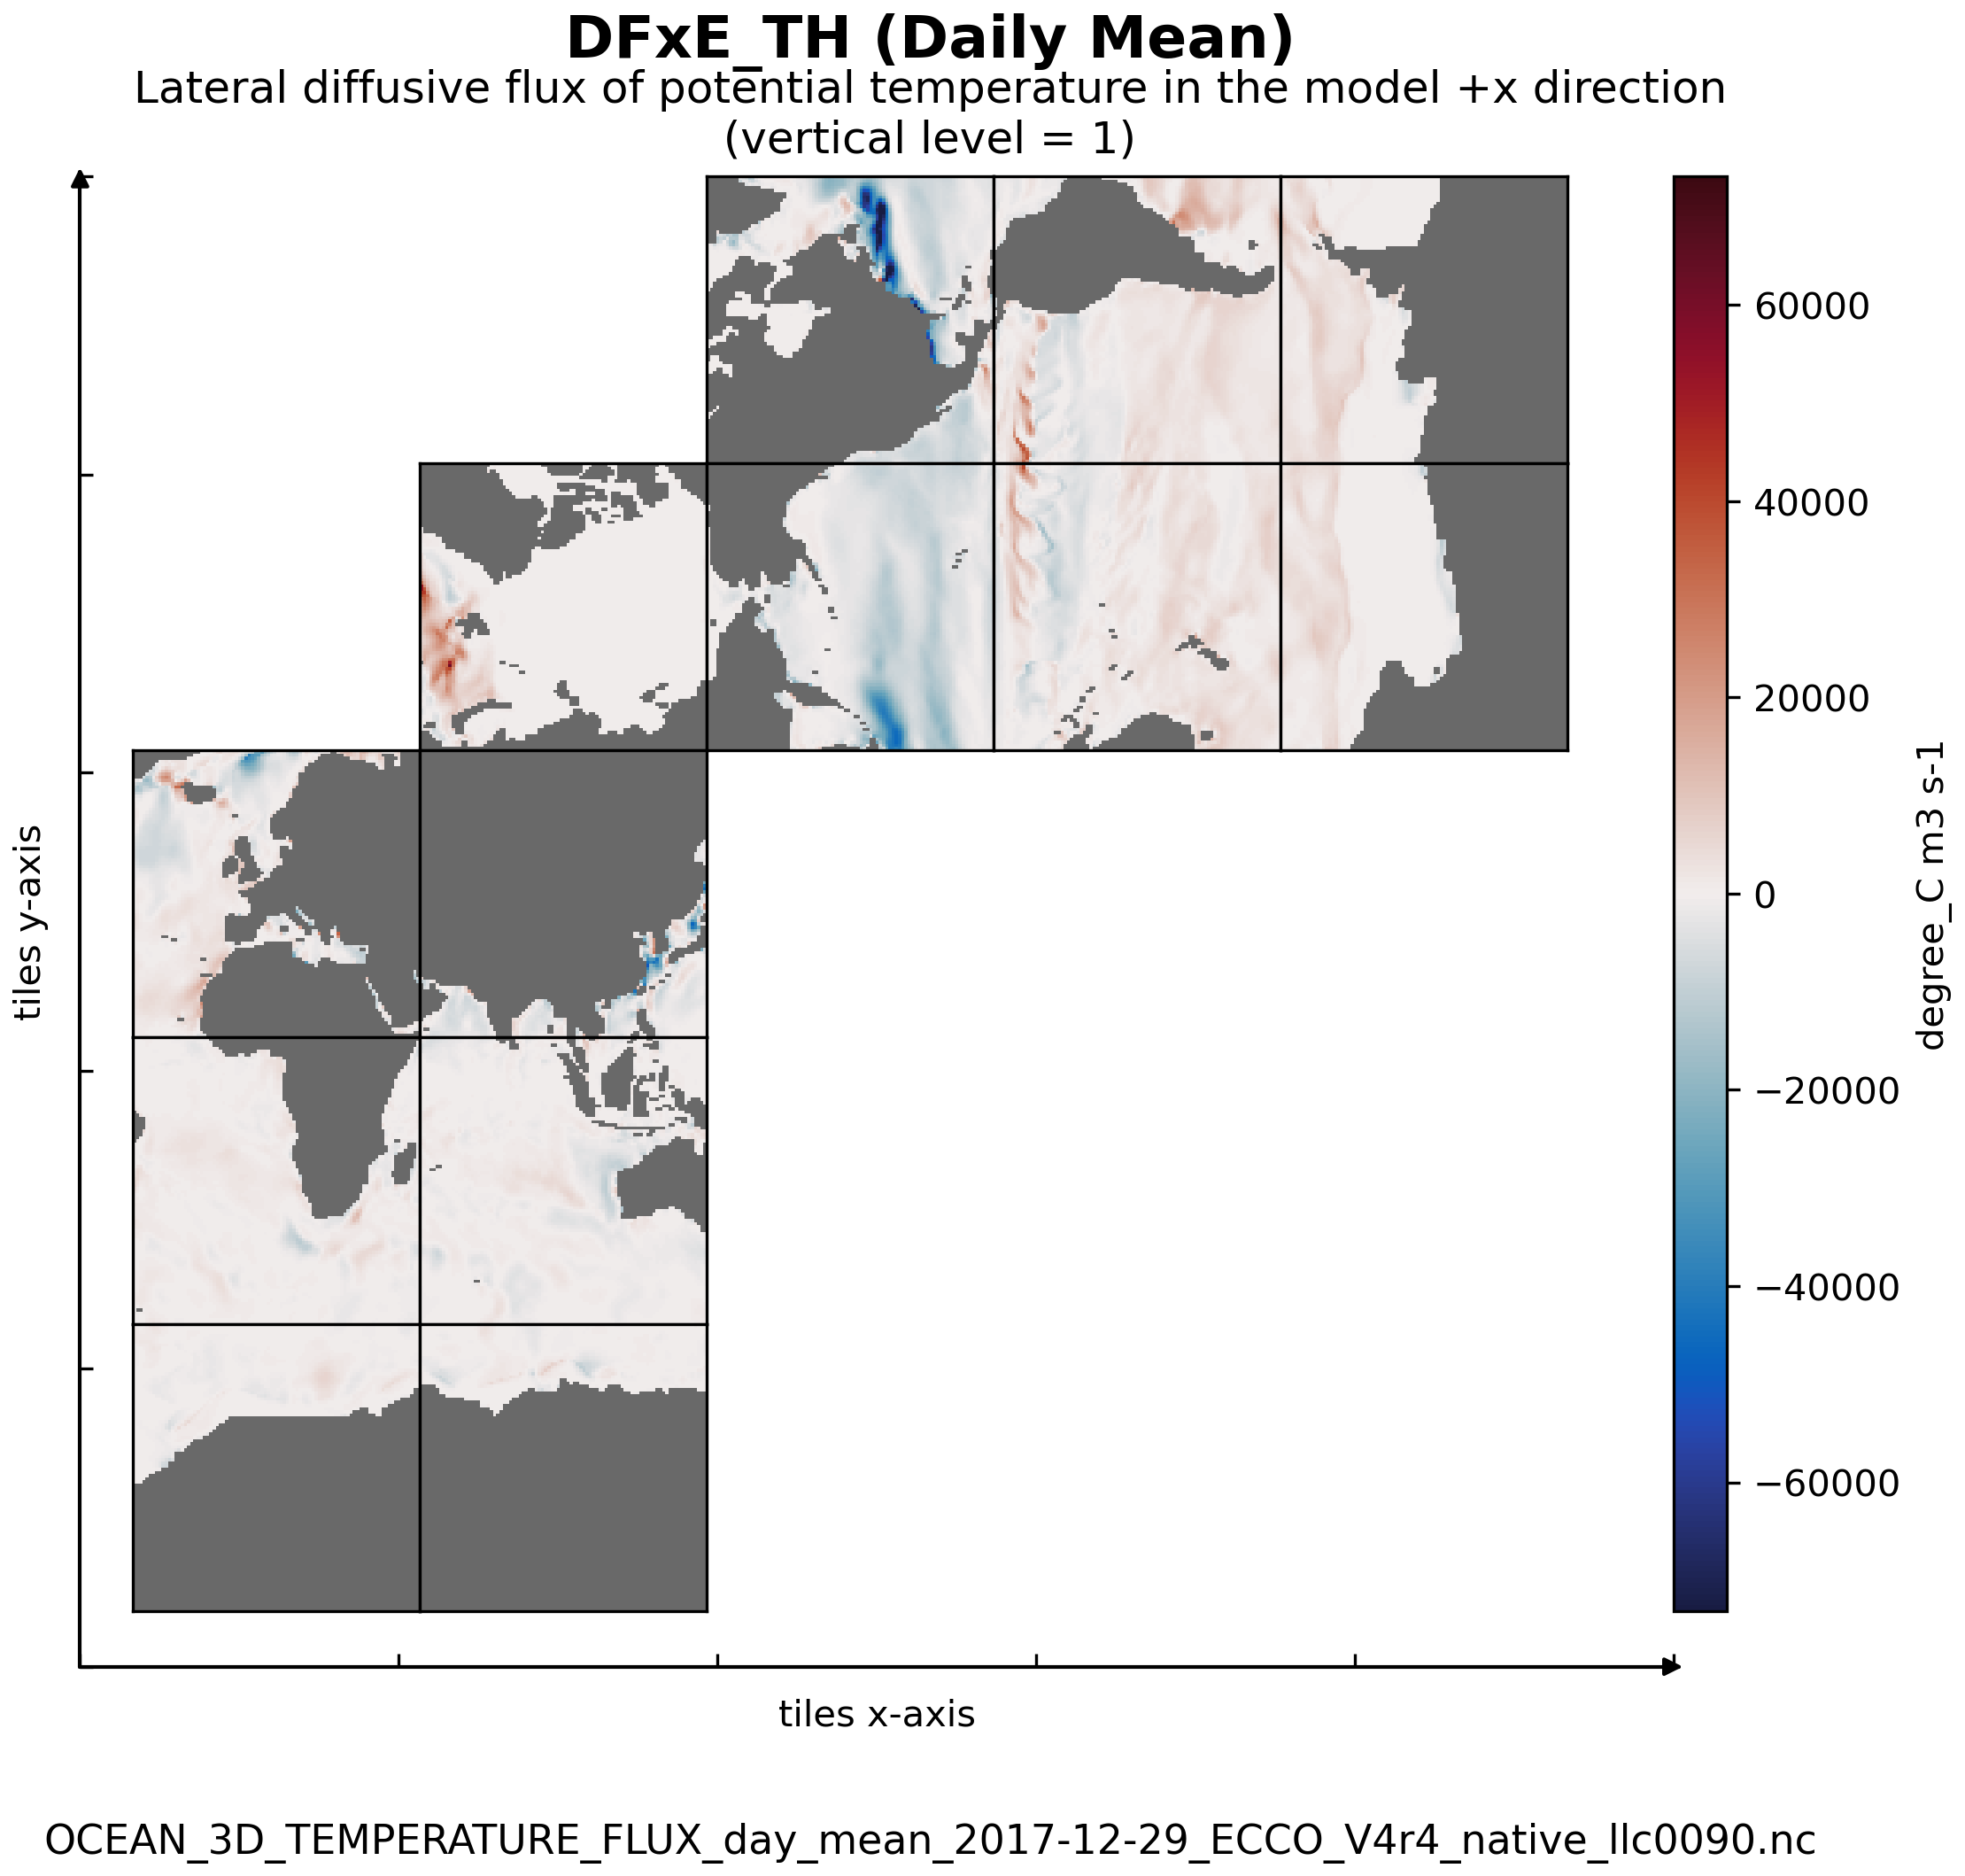
\includegraphics[scale=0.55]{../images/plots/v4r4/native_plots/Ocean_Three-Dimensional_Potential_Temperature_Fluxes/DFxE_TH.png}
\caption{Dataset: OCEAN\_3D\_TEMPERATURE\_FLUX, Variable: DFxE\_TH}
\label{tab:table-OCEAN_3D_TEMPERATURE_FLUX_DFxE_TH-Plot}
\end{figure}
\newpage
\pagebreak
\subsubsection{Native Variable: DFyE\_TH}
\begin{longtable}{|m{0.06\textwidth}|m{0.3\textwidth}|m{0.45\textwidth}|m{0.12\textwidth}|}
\caption{Attributes description of the variable 'DFyE\_TH' from OCEAN\_3D\_TEMPERATURE\_FLUX's  dataset.}
\label{tab:table-OCEAN_3D_TEMPERATURE_FLUX_DFyE_TH} \\ 
\hline \endhead \hline \endfoot
\rowcolor{lightgray} \textbf{Storage Type} & \textbf{Variable Name} & \textbf{Description} & \textbf{Unit} \\ \hline
float32 & DFyE\_TH & Lateral diffusive flux of potential temperature in the model +y direction. & degree\_C m3 s-1 \\ \hline
\multicolumn{4}{|c|}{\cellcolor{lightgray}{\textbf{Description of the variable in Common Data language (CDL)}}} \\ \hline
\multicolumn{4}{|c|}{\fontfamily{lmtt}\selectfont{\makecell{\parbox{.95\textwidth}{\vspace*{0.25cm} \footnotesize{float32 DFyE\_TH(time, k, tile, j\_g, i)\\
\hspace*{0.5cm}DFyE\_TH: \_FillValue = 9.96921e+36\\
\hspace*{0.5cm}DFyE\_TH: coordinates = time Z\\
\hspace*{0.5cm}DFyE\_TH: coverage\_content\_type = modelResult\\
\hspace*{0.5cm}DFyE\_TH: direction = >0 increases potential temperature (THETA)\\
\hspace*{0.5cm}DFyE\_TH: long\_name = Lateral diffusive flux of potential temperature in the model +y direction.\\
\hspace*{0.5cm}DFyE\_TH: mate = DFxE TH\\
\hspace*{0.5cm}DFyE\_TH: units = degree C m3 s-1\\
\hspace*{0.5cm}DFyE\_TH: valid\_max = 1053781.25\\
\hspace*{0.5cm}DFyE\_TH: valid\_min = -421044.78125\\
}}}}} \\ \hline
\rowcolor{lightgray} \multicolumn{4}{|c|}{\textbf{Comments}} \\ \hline
\multicolumn{4}{|p{1\textwidth}|}{\footnotesize{{Lateral diffusive flux of potential temperature (theta) in the +y direction through the 'v' face of the tracer cell on the native model grid. note: in the arakawa-c grid, horizontal flux quantities are staggered relative to the tracer cells with indexing such that +dfye\_th(i,j\_g,k) corresponds to +y fluxes through the 'v' face of the tracer cell at (i,j,k). also, the model +y direction does not necessarily correspond to the geographical north-south direction because the x and y axes of the model's curvilinear lat-lon-cap (llc) grid have arbitrary orientations which vary within and across tiles.}}} \\ \hline
\end{longtable}

\begin{figure}[H]
\centering
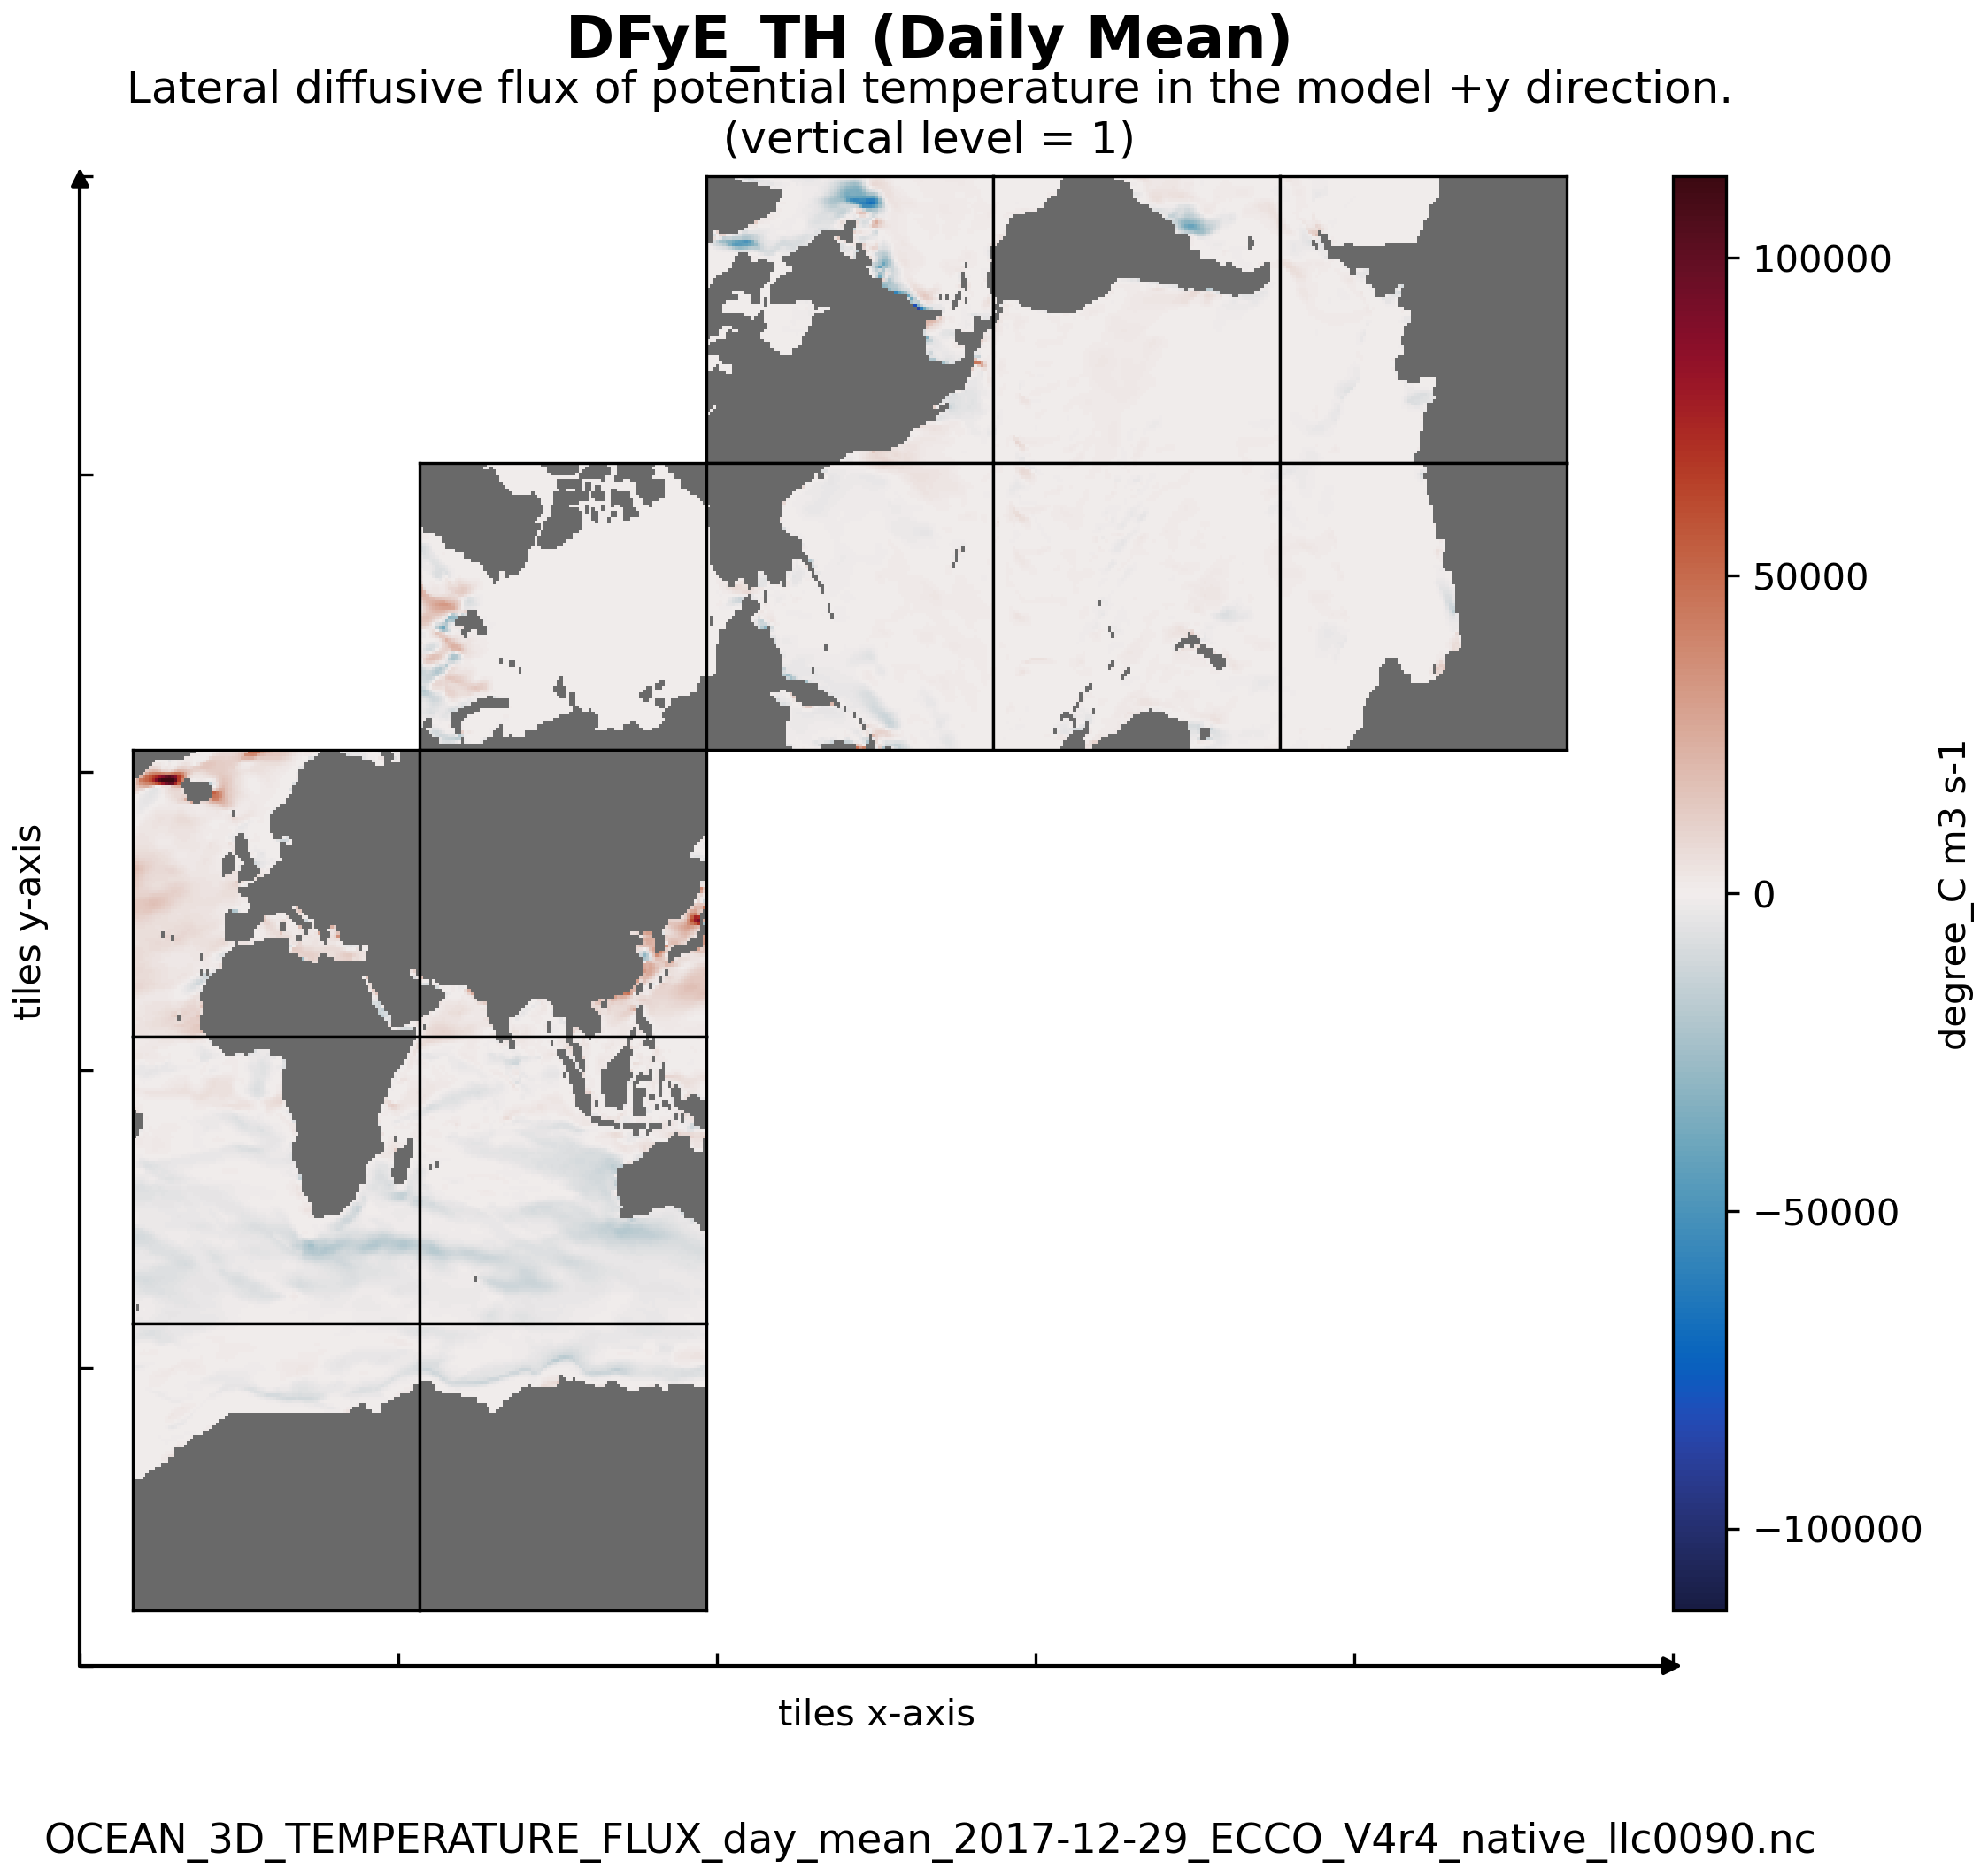
\includegraphics[scale=0.55]{../images/plots/v4r4/native_plots/Ocean_Three-Dimensional_Potential_Temperature_Fluxes/DFyE_TH.png}
\caption{Dataset: OCEAN\_3D\_TEMPERATURE\_FLUX, Variable: DFyE\_TH}
\label{tab:table-OCEAN_3D_TEMPERATURE_FLUX_DFyE_TH-Plot}
\end{figure}
\newpage
\subsection{Native dataset of OCEAN\_3D\_VOLUME\_FLUX}
\newp
\subsubsection{Overview}
This dataset provides three-dimensional ocean volume fluxes on the lat-lon-cap 90 (llc90) native model grid from the ECCO Version 4 Release 4 (V4r4) ocean and sea-ice state estimate. The dataset is provided on daily-average and monthly-average time resolution. Volume flux in +x direction = UVELMASS drF dyG. Volume flux in +y direction = VVELMASS drF dxG. Volume flux in +z direction = WVELMASS drA. 
\begin{longtable}{|m{0.15\textwidth}|m{0.64\textwidth}|m{0.12\textwidth}|}
\caption{Coordinates and Variables in the dataset OCEAN\_3D\_VOLUME\_FLUX}
\label{tab:table-OCEAN_3D_VOLUME_FLUX-fields} \\ 
\hline \endhead \hline \endfoot
\rowcolor{lightgray} \multicolumn{1}{|c|}{\textbf{Coordinates}} & \multicolumn{1}{|c|}{\textbf{Description of data coordinates}} &  \multicolumn{1}{|c|}{\textbf{Unit}}\\ \hline
i &Grid index in x for variables at tracer and 'v' locations &--none--  \\ \hline
i\_g &Grid index in x for variables at 'u' and 'g' locations &--none--  \\ \hline
j &Grid index in y for variables at tracer and 'u' locations &--none--  \\ \hline
j\_g &Grid index in y for variables at 'v' and 'g' locations &--none--  \\ \hline
k &Grid index in z for tracer variables &--none--  \\ \hline
k\_u &Grid index in z corresponding to the bottom face of tracer grid cells ('w' locations) &--none--  \\ \hline
k\_l &Grid index in z corresponding to the top face of tracer grid cells ('w' locations) &--none--  \\ \hline
k\_p1 &Grid index in z for variables at 'w' locations &--none--  \\ \hline
tile &Lat-lon-cap tile index &--none--  \\ \hline
time &Center time of averaging period &--none--  \\ \hline
XC &Longitude of tracer grid cell center &degrees\_east  \\ \hline
YC &Latitude of tracer grid cell center &degrees\_north  \\ \hline
XG &Longitude of 'southwest' corner of tracer grid cell &degrees\_east  \\ \hline
YG &Latitude of 'southwest' corner of tracer grid cell &degrees\_north  \\ \hline
Z &Depth of tracer grid cell center &m  \\ \hline
Zp1 &Depth of tracer grid cell interface &m  \\ \hline
Zu &Depth of the bottom face of tracer grid cells &m  \\ \hline
Zl &Depth of the top face of tracer grid cells &m  \\ \hline
time\_bnds &Time bounds of averaging period &--none--  \\ \hline
XC\_bnds &Longitudes of tracer grid cell corners &--none--  \\ \hline
YC\_bnds &Latitudes of tracer grid cell corners &--none--  \\ \hline
Z\_bnds &Depths of tracer grid cell upper and lower interfaces &--none--  \\ \hline
\rowcolor{lightgray} \multicolumn{1}{|c|}{\textbf{Variables}} & \multicolumn{1}{|c|}{\textbf{Description of data variables}} &  \multicolumn{1}{|c|}{\textbf{Unit}}\\ \hline
UVELMASS &Horizontal velocity in the model +x direction per unit area of the grid cell 'u' face &m s-1  \\ \hline
VVELMASS &Horizontal velocity in the model +y direction per unit area of the grid cell 'v' face &m s-1 m3 m-3  \\ \hline
WVELMASS &Grid cell face-averaged vertical velocity in the model +z direction. &m s-1  \\ \hline
\end{longtable}

\newp
\pagebreak
\subsubsection{Native Variable: UVELMASS}
\begin{longtable}{|m{0.06\textwidth}|m{0.3\textwidth}|m{0.45\textwidth}|m{0.12\textwidth}|}
\caption{Attributes description of the variable 'UVELMASS' from OCEAN\_3D\_VOLUME\_FLUX's  dataset.}
\label{tab:table-OCEAN_3D_VOLUME_FLUX_UVELMASS} \\ 
\hline \endhead \hline \endfoot
\rowcolor{lightgray} \textbf{Storage Type} & \textbf{Variable Name} & \textbf{Description} & \textbf{Unit} \\ \hline
float32 & UVELMASS & Horizontal velocity in the model +x direction per unit area of the grid cell 'u' face & m s-1 \\ \hline
\multicolumn{4}{|c|}{\cellcolor{lightgray}{\textbf{Description of the variable in Common Data language (CDL)}}} \\ \hline
\multicolumn{4}{|c|}{\fontfamily{lmtt}\selectfont{\makecell{\parbox{.95\textwidth}{\vspace*{0.25cm} \footnotesize{float32 UVELMASS(time, k, tile, j, i\_g)\\
\hspace*{0.5cm}UVELMASS: \_FillValue = 9.96921e+36\\
\hspace*{0.5cm}UVELMASS: coordinates = Z time\\
\hspace*{0.5cm}UVELMASS: coverage\_content\_type = modelResult\\
\hspace*{0.5cm}UVELMASS: direction = >0 increases volume\\
\hspace*{0.5cm}UVELMASS: long\_name = Horizontal velocity in the model +x direction per unit area of the grid cell u face\\
\hspace*{0.5cm}UVELMASS: mate = VVELMASS\\
\hspace*{0.5cm}UVELMASS: units = m s-1\\
\hspace*{0.5cm}UVELMASS: valid\_max = 2.0377726554870605\\
\hspace*{0.5cm}UVELMASS: valid\_min = -2.115365505218506\\
}}}}} \\ \hline
\rowcolor{lightgray} \multicolumn{4}{|c|}{\textbf{Comments}} \\ \hline
\multicolumn{4}{|p{1\textwidth}|}{\footnotesize{{Horizontal velocity in the model +x direction averaged over the area of the tracer grid cell 'u' face on the native model grid ('u' grid cell face area = drf dyg). accounts for partial cells (hfacw < 1) and for time-varying grid cell thickness (z* coordinate system). volume flux in +x = uvelmass drf dyg. note: in the arakawa-c grid, horizontal velocities are staggered relative to the tracer cells with indexing such that +uvelmass(i,j,k) corresponds to +x fluxes through the 'u' face of the tracer cell at (i,j,k). uvelmass can be used for volume flux calculations because it accounts for the grid cell thicknesses variations in the +x direction (hfacw) with time (z* coordinate system). also, the model +x direction does not necessarily correspond to the geographical east-west direction because the x and y axes of the model's curvilinear lat-lon-cap (llc) grid have arbitrary orientations which vary within and across tiles. see vvelmass and wvelmass}}} \\ \hline
\end{longtable}

\begin{figure}[H]
\centering
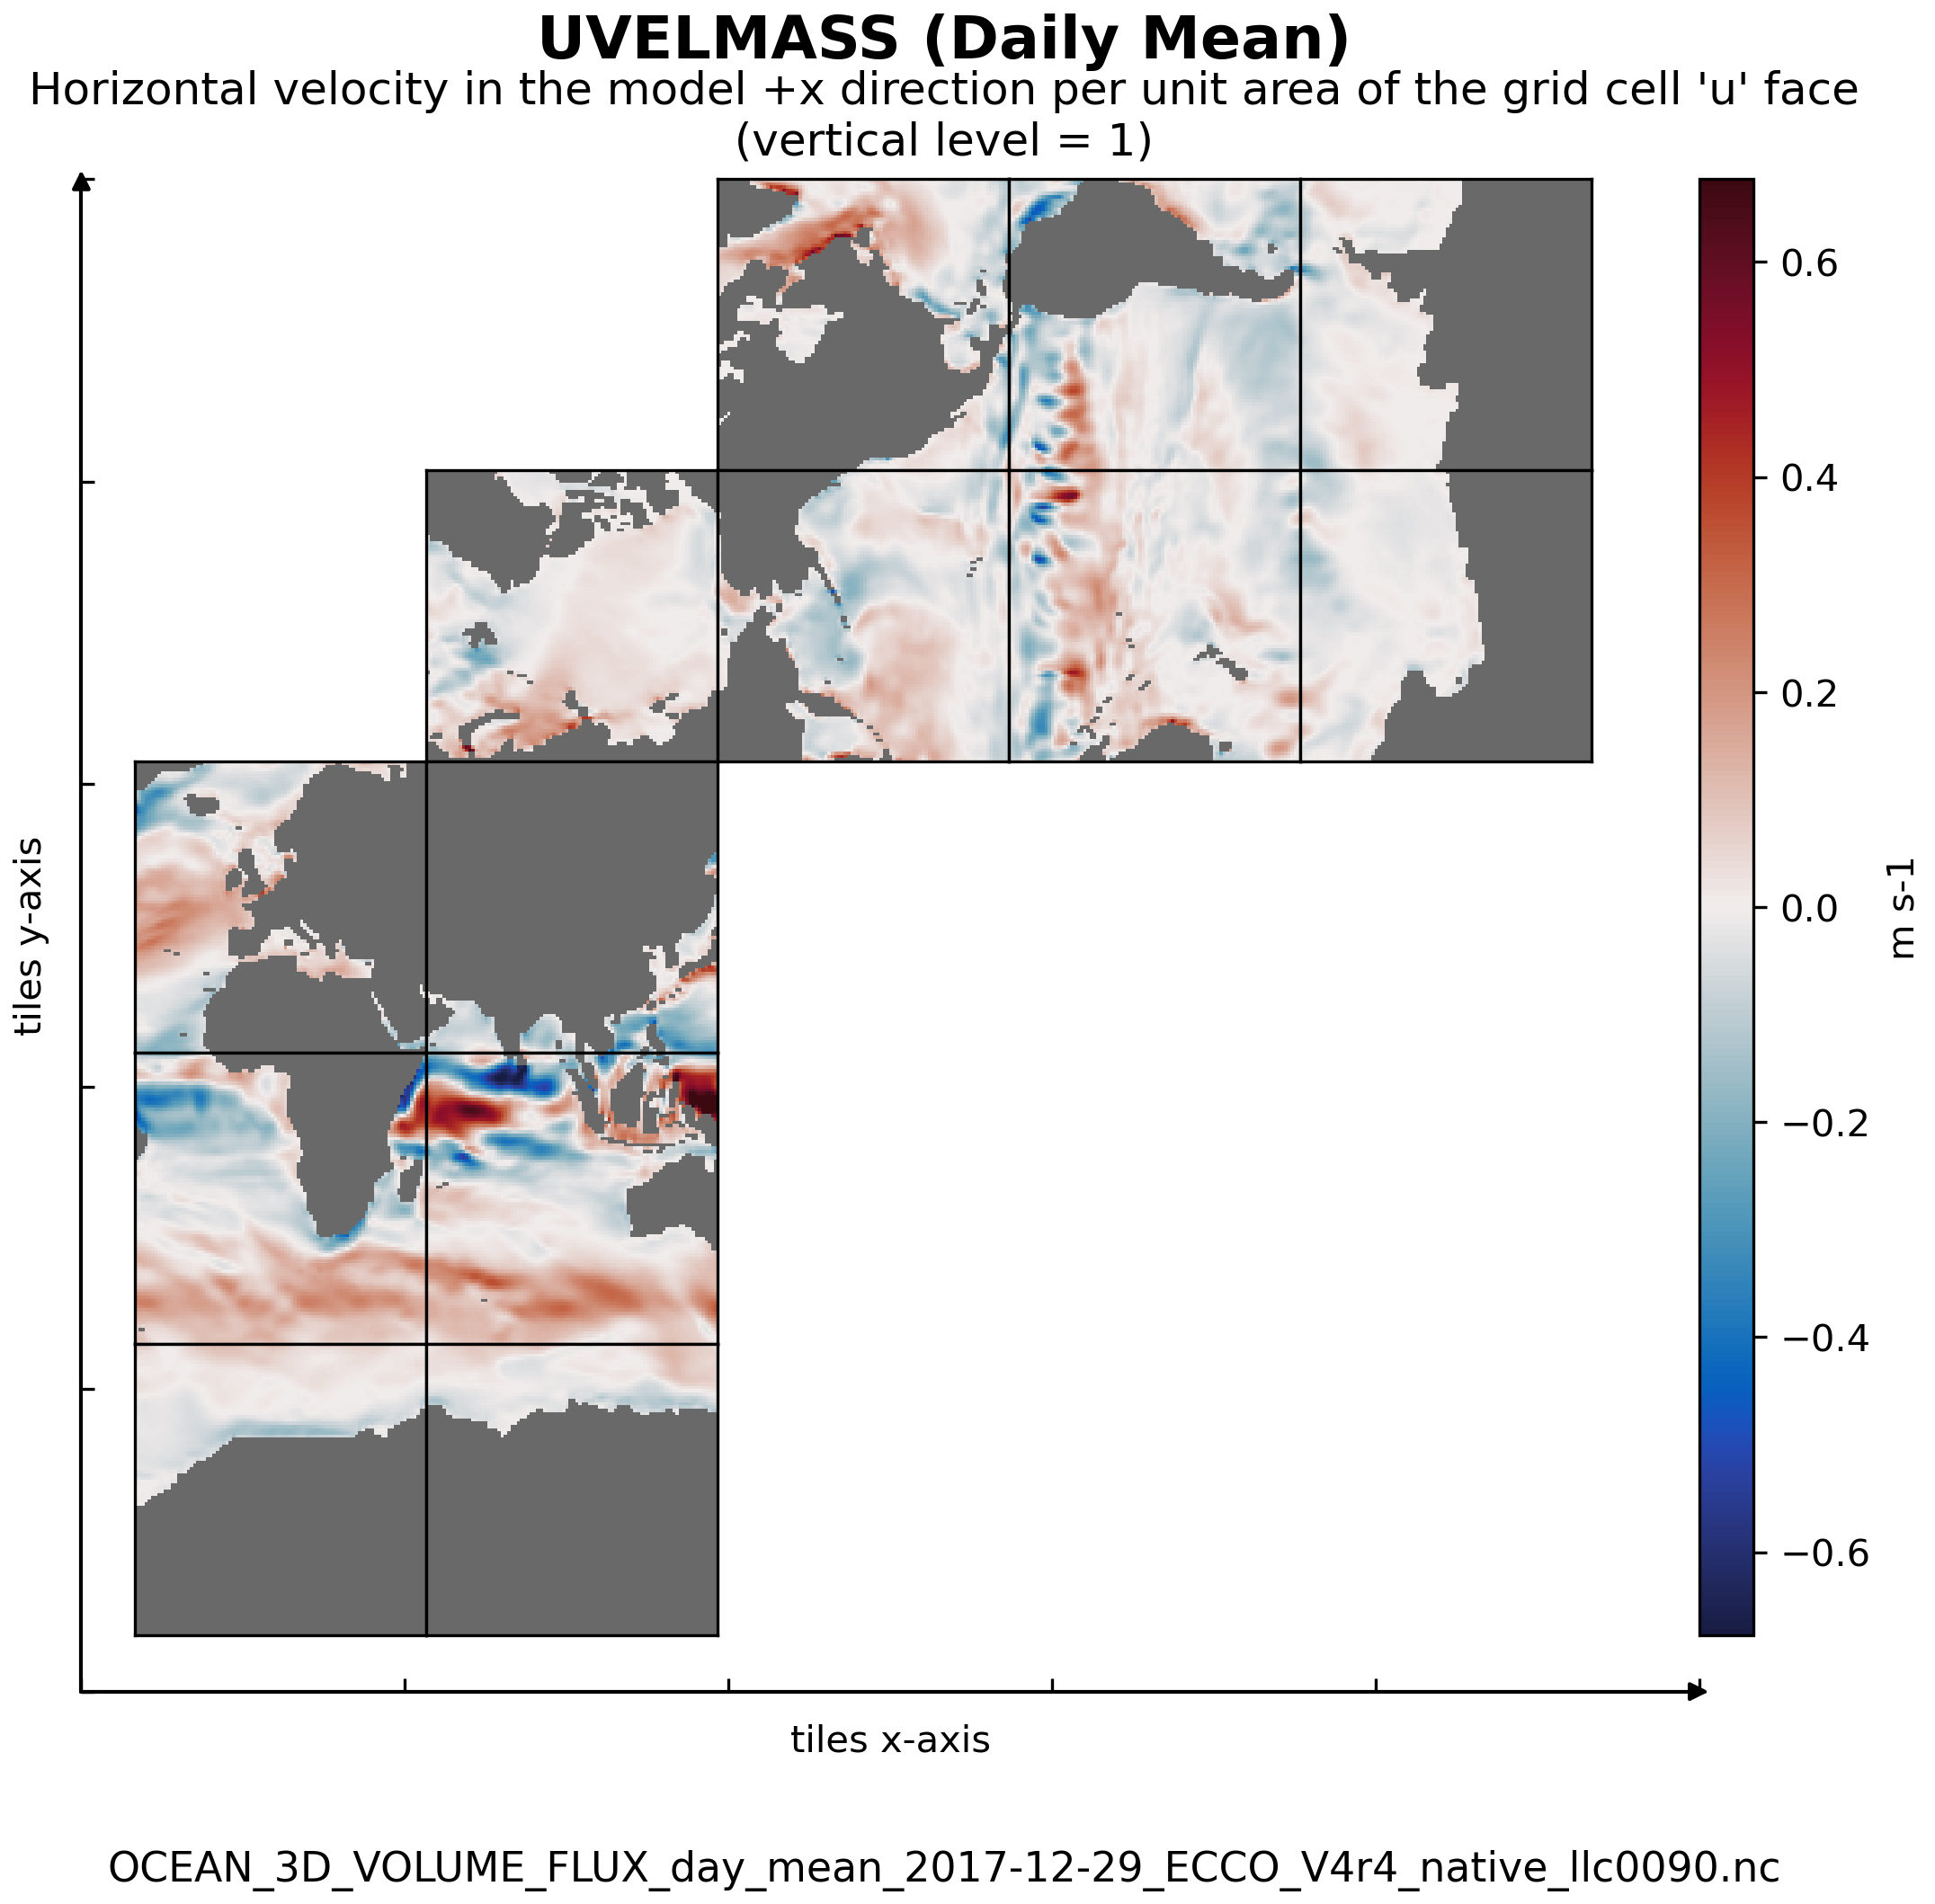
\includegraphics[scale=0.55]{../images/plots/v4r4/native_plots/Ocean_Three-Dimensional_Volume_Fluxes/UVELMASS.png}
\caption{Dataset: OCEAN\_3D\_VOLUME\_FLUX, Variable: UVELMASS}
\label{tab:table-OCEAN_3D_VOLUME_FLUX_UVELMASS-Plot}
\end{figure}
\newpage
\pagebreak
\subsubsection{Native Variable: VVELMASS}
\begin{longtable}{|m{0.06\textwidth}|m{0.3\textwidth}|m{0.45\textwidth}|m{0.12\textwidth}|}
\caption{Attributes description of the variable 'VVELMASS' from OCEAN\_3D\_VOLUME\_FLUX's  dataset.}
\label{tab:table-OCEAN_3D_VOLUME_FLUX_VVELMASS} \\ 
\hline \endhead \hline \endfoot
\rowcolor{lightgray} \textbf{Storage Type} & \textbf{Variable Name} & \textbf{Description} & \textbf{Unit} \\ \hline
float32 & VVELMASS & Horizontal velocity in the model +y direction per unit area of the grid cell 'v' face & m s-1 m3 m-3 \\ \hline
\multicolumn{4}{|c|}{\cellcolor{lightgray}{\textbf{Description of the variable in Common Data language (CDL)}}} \\ \hline
\multicolumn{4}{|c|}{\fontfamily{lmtt}\selectfont{\makecell{\parbox{.95\textwidth}{\vspace*{0.25cm} \footnotesize{float32 VVELMASS(time, k, tile, j\_g, i)\\
\hspace*{0.5cm}VVELMASS: \_FillValue = 9.96921e+36\\
\hspace*{0.5cm}VVELMASS: coordinates = Z time\\
\hspace*{0.5cm}VVELMASS: coverage\_content\_type = modelResult\\
\hspace*{0.5cm}VVELMASS: direction = >0 increases volume\\
\hspace*{0.5cm}VVELMASS: long\_name = Horizontal velocity in the model +y direction per unit area of the grid cell v face\\
\hspace*{0.5cm}VVELMASS: mate = UVELMASS\\
\hspace*{0.5cm}VVELMASS: units = m s-1 m3 m-3\\
\hspace*{0.5cm}VVELMASS: valid\_max = 1.9216758012771606\\
\hspace*{0.5cm}VVELMASS: valid\_min = -1.7897182703018188\\
}}}}} \\ \hline
\rowcolor{lightgray} \multicolumn{4}{|c|}{\textbf{Comments}} \\ \hline
\multicolumn{4}{|p{1\textwidth}|}{\footnotesize{{Horizontal velocity in the model +y direction averaged over the area of the tracer grid cell 'v' face on the native model grid ('v' grid cell face area = drf dxg). accounts for partial cells (hfacs < 1) and for time-varying grid cell thickness (z* coordinate system). volume flux in +y = vvelmass drf dxg. note: in the arakawa-c grid, horizontal velocities are staggered relative to the tracer cells with indexing such that +vvelmass(i,j,k) corresponds to +y fluxes through the 'v' face of the tracer cell at (i,j,k). vvelmass can be used for volume flux calculations because it accounts for grid cell thicknesses variations in the +y direction (hfacs) with time (z* coordinate system). also, the model +y direction does not necessarily correspond to the geographical north-south direction because the x and y axes of the model's curvilinear lat-lon-cap (llc) grid have arbitrary orientations which vary within and across tiles. see uvelmass and wvelmass.}}} \\ \hline
\end{longtable}

\begin{figure}[H]
\centering
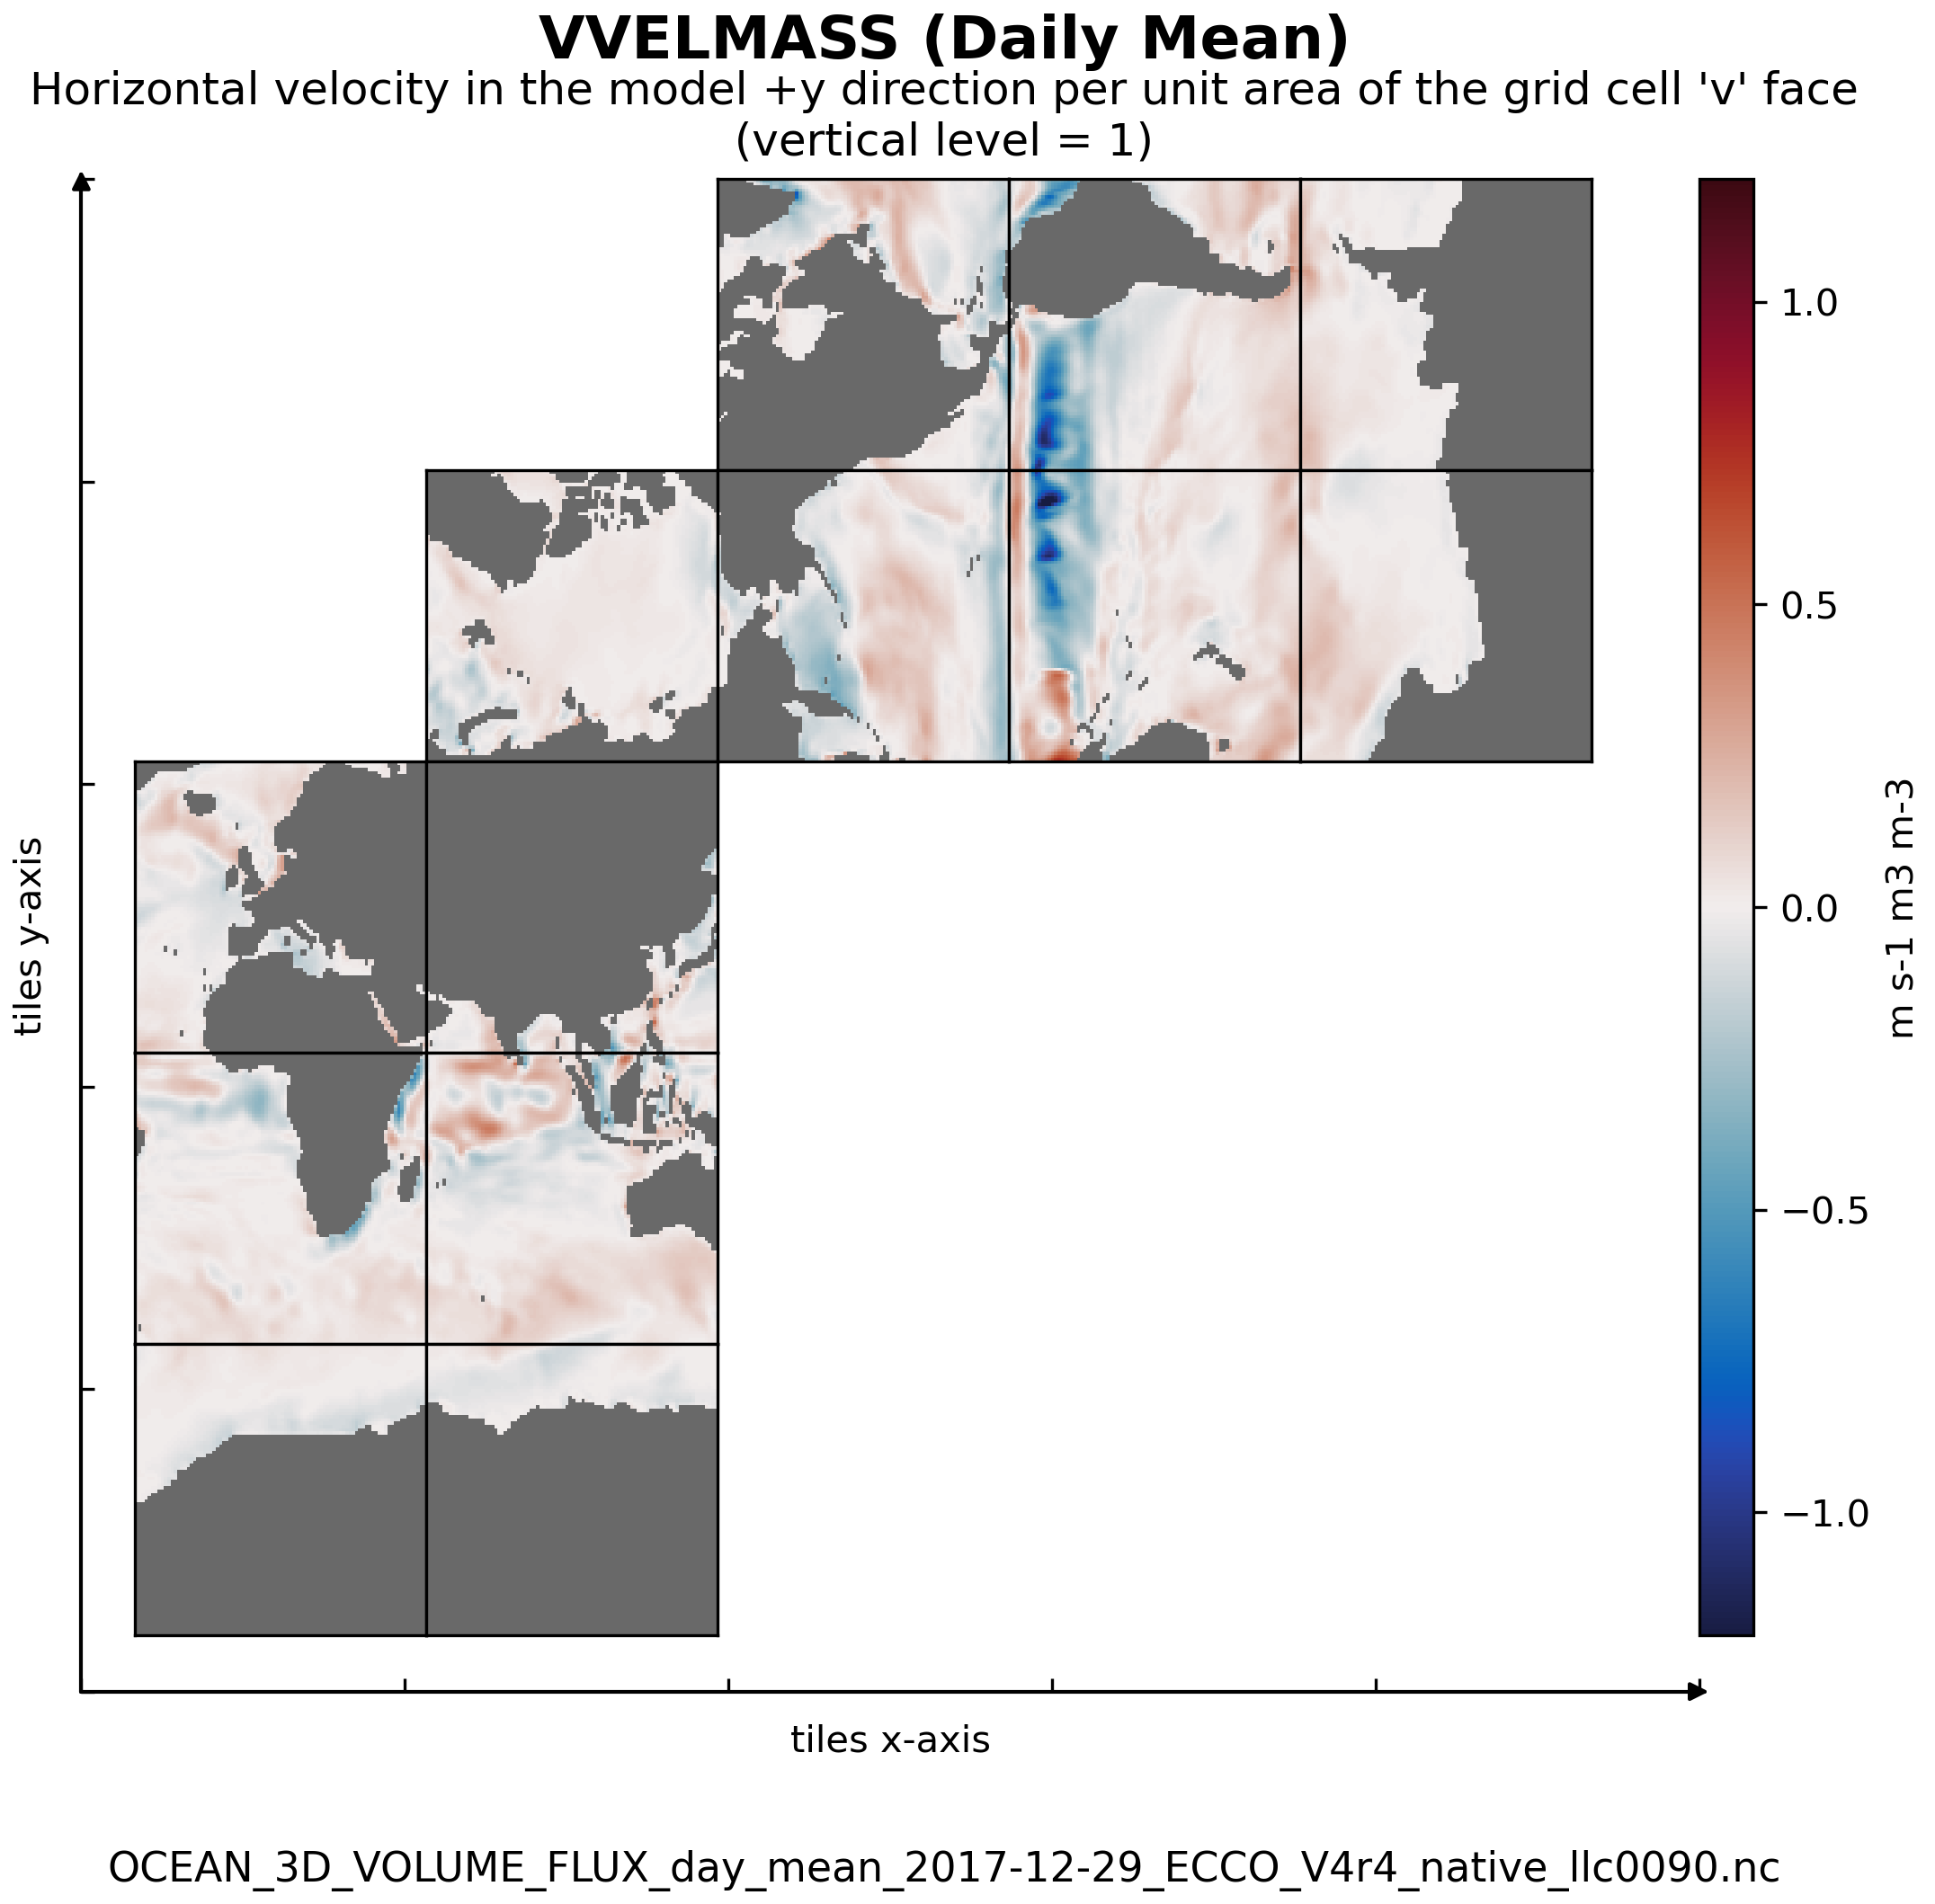
\includegraphics[scale=0.55]{../images/plots/v4r4/native_plots/Ocean_Three-Dimensional_Volume_Fluxes/VVELMASS.png}
\caption{Dataset: OCEAN\_3D\_VOLUME\_FLUX, Variable: VVELMASS}
\label{tab:table-OCEAN_3D_VOLUME_FLUX_VVELMASS-Plot}
\end{figure}
\newpage
\pagebreak
\subsubsection{Native Variable: WVELMASS}
\begin{longtable}{|m{0.06\textwidth}|m{0.3\textwidth}|m{0.45\textwidth}|m{0.12\textwidth}|}
\caption{Attributes description of the variable 'WVELMASS' from OCEAN\_3D\_VOLUME\_FLUX's  dataset.}
\label{tab:table-OCEAN_3D_VOLUME_FLUX_WVELMASS} \\ 
\hline \endhead \hline \endfoot
\rowcolor{lightgray} \textbf{Storage Type} & \textbf{Variable Name} & \textbf{Description} & \textbf{Unit} \\ \hline
float32 & WVELMASS & Grid cell face-averaged vertical velocity in the model +z direction. & m s-1 \\ \hline
\multicolumn{4}{|c|}{\cellcolor{lightgray}{\textbf{Description of the variable in Common Data language (CDL)}}} \\ \hline
\multicolumn{4}{|c|}{\fontfamily{lmtt}\selectfont{\makecell{\parbox{.95\textwidth}{\vspace*{0.25cm} \footnotesize{float32 WVELMASS(time, k\_l, tile, j, i)\\
\hspace*{0.5cm}WVELMASS: \_FillValue = 9.96921e+36\\
\hspace*{0.5cm}WVELMASS: coordinates = YC Zl time XC\\
\hspace*{0.5cm}WVELMASS: coverage\_content\_type = modelResult\\
\hspace*{0.5cm}WVELMASS: direction = >0 decreases volume\\
\hspace*{0.5cm}WVELMASS: long\_name = Grid cell face-averaged vertical velocity in the model +z direction.\\
\hspace*{0.5cm}WVELMASS: standard\_name = upward sea water velocity\\
\hspace*{0.5cm}WVELMASS: units = m s-1\\
\hspace*{0.5cm}WVELMASS: valid\_max = 0.0016380994347855449\\
\hspace*{0.5cm}WVELMASS: valid\_min = -0.0023150660563260317\\
}}}}} \\ \hline
\rowcolor{lightgray} \multicolumn{4}{|c|}{\textbf{Comments}} \\ \hline
\multicolumn{4}{|p{1\textwidth}|}{\footnotesize{{Vertical velocity in the +z direction at the top 'w' face of the tracer cell on the native model grid. volume flux in +z = wvelmass dra. note: in the arakawa-c grid, vertical velocities are staggered relative to the tracer cells with indexing such that +wvelmass(i,j,k) corresponds to upward +z motion through the top 'w' face of the tracer cell at (i,j,k). unlike uvelmass and vvelmass, wvelmass is not scaled by a time-varying open water fraction because the open water fraction of the 'w' face is always 1, thus wvelmass is identical to wvel.}}} \\ \hline
\end{longtable}

\begin{figure}[H]
\centering
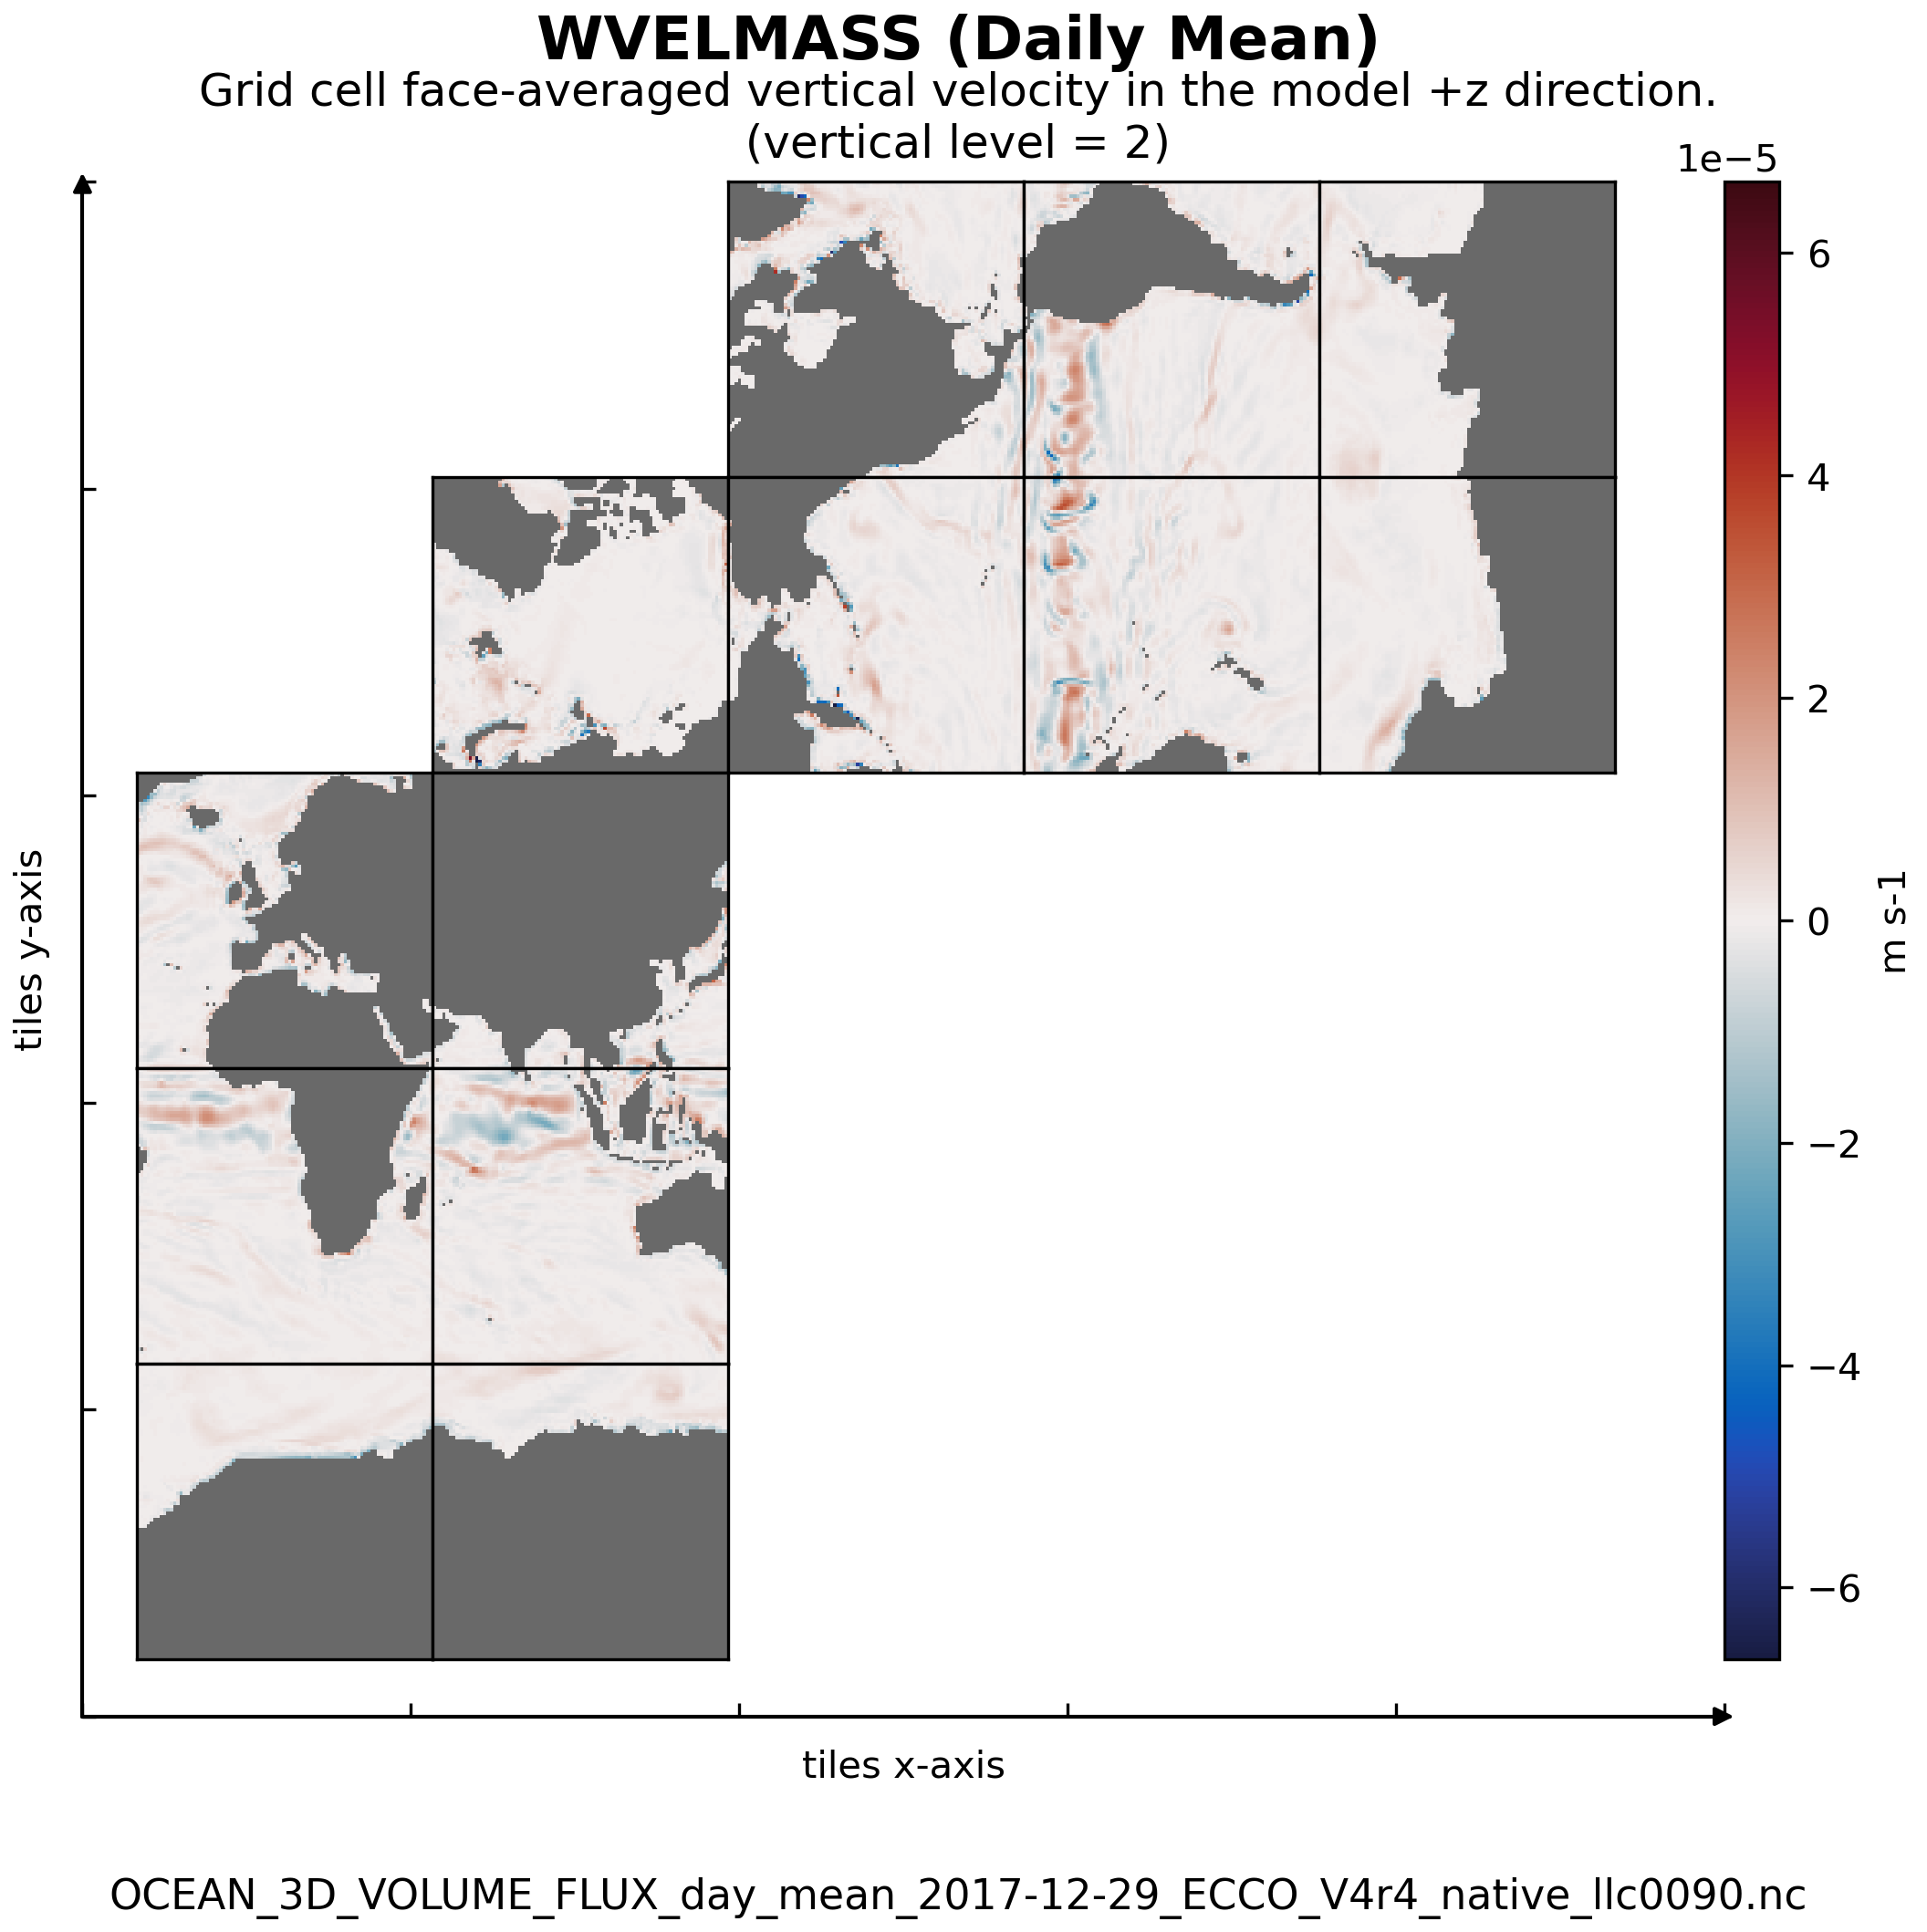
\includegraphics[scale=0.55]{../images/plots/v4r4/native_plots/Ocean_Three-Dimensional_Volume_Fluxes/WVELMASS.png}
\caption{Dataset: OCEAN\_3D\_VOLUME\_FLUX, Variable: WVELMASS}
\label{tab:table-OCEAN_3D_VOLUME_FLUX_WVELMASS-Plot}
\end{figure}
\newpage
\subsection{Native dataset of OCEAN\_AND\_ICE\_SURFACE\_FW\_FLUX}
\newp
\subsubsection{Overview}
This dataset provides 2D fields of ocean and sea-ice surface freshwater fluxes on the lat-lon-cap 90 (llc90) native model grid from the ECCO Version 4 Release 4 (V4r4) ocean and sea-ice state estimate. The dataset is provided on daily-average and monthly-average time resolution. 
\begin{longtable}{|m{0.15\textwidth}|m{0.64\textwidth}|m{0.12\textwidth}|}
\caption{Coordinates and Variables in the dataset OCEAN\_AND\_ICE\_SURFACE\_FW\_FLUX}
\label{tab:table-OCEAN_AND_ICE_SURFACE_FW_FLUX-fields} \\ 
\hline \endhead \hline \endfoot
\rowcolor{lightgray} \multicolumn{1}{|c|}{\textbf{Coordinates}} & \multicolumn{1}{|c|}{\textbf{Description of data coordinates}} &  \multicolumn{1}{|c|}{\textbf{Unit}}\\ \hline
i &Grid index in x for variables at tracer and 'v' locations &--none--  \\ \hline
i\_g &Grid index in x for variables at 'u' and 'g' locations &--none--  \\ \hline
j &Grid index in y for variables at tracer and 'u' locations &--none--  \\ \hline
j\_g &Grid index in y for variables at 'v' and 'g' locations &--none--  \\ \hline
tile &Lat-lon-cap tile index &--none--  \\ \hline
time &Center time of averaging period &--none--  \\ \hline
XC &Longitude of tracer grid cell center &degrees\_east  \\ \hline
YC &Latitude of tracer grid cell center &degrees\_north  \\ \hline
XG &Longitude of 'southwest' corner of tracer grid cell &degrees\_east  \\ \hline
YG &Latitude of 'southwest' corner of tracer grid cell &degrees\_north  \\ \hline
time\_bnds &Time bounds of averaging period &--none--  \\ \hline
XC\_bnds &Longitudes of tracer grid cell corners &--none--  \\ \hline
YC\_bnds &Latitudes of tracer grid cell corners &--none--  \\ \hline
\rowcolor{lightgray} \multicolumn{1}{|c|}{\textbf{Variables}} & \multicolumn{1}{|c|}{\textbf{Description of data variables}} &  \multicolumn{1}{|c|}{\textbf{Unit}}\\ \hline
EXFpreci &Precipitation rate &m s-1  \\ \hline
EXFevap &Open ocean evaporation rate &m s-1  \\ \hline
EXFroff &River runoff &m s-1  \\ \hline
SIsnPrcp &Snow precipitation on sea-ice &kg m-2 s-1  \\ \hline
EXFempmr &Open ocean net surface freshwater flux from precipitation, evaporation, and runoff &m s-1  \\ \hline
oceFWflx &Net freshwater flux into the ocean &kg m-2 s-1  \\ \hline
SIatmFW &Net freshwater flux into the open ocean, sea-ice, and snow &kg m-2 s-1  \\ \hline
SFLUX &Rate of change of total ocean salinity per m2 accounting for mass fluxes. &g m-2 s-1  \\ \hline
SIacSubl &Freshwater flux to the atmosphere due to sublimation-deposition of snow or ice &kg m-2 s-1  \\ \hline
SIrsSubl &Residual sublimation freshwater flux &kg m-2 s-1  \\ \hline
SIfwThru &Precipitation through sea-ice &kg m-2 s-1  \\ \hline
\end{longtable}

\newp
\pagebreak
\subsubsection{Native Variable: EXFempmr}
\begin{longtable}{|m{0.06\textwidth}|m{0.3\textwidth}|m{0.45\textwidth}|m{0.12\textwidth}|}
\caption{Attributes description of the variable 'EXFempmr' from OCEAN\_AND\_ICE\_SURFACE\_FW\_FLUX's  dataset.}
\label{tab:table-OCEAN_AND_ICE_SURFACE_FW_FLUX_EXFempmr} \\ 
\hline \endhead \hline \endfoot
\rowcolor{lightgray} \textbf{Storage Type} & \textbf{Variable Name} & \textbf{Description} & \textbf{Unit} \\ \hline
float32 & EXFempmr & Open ocean net surface freshwater flux from precipitation, evaporation, and runoff & m s-1 \\ \hline
\multicolumn{4}{|c|}{\cellcolor{lightgray}{\textbf{Description of the variable in Common Data language (CDL)}}} \\ \hline
\multicolumn{4}{|c|}{\fontfamily{lmtt}\selectfont{\makecell{\parbox{.95\textwidth}{\vspace*{0.25cm} \footnotesize{float32 EXFempmr(time, tile, j, i)\\
\hspace*{0.5cm}EXFempmr: \_FillValue = 9.96921e+36\\
\hspace*{0.5cm}EXFempmr: coordinates = YC XC time\\
\hspace*{0.5cm}EXFempmr: coverage\_content\_type = modelResult\\
\hspace*{0.5cm}EXFempmr: direction = >0 increases salinity (SALT)\\
\hspace*{0.5cm}EXFempmr: long\_name = Open ocean net surface freshwater flux from precipitation, evaporation, and runoff\\
\hspace*{0.5cm}EXFempmr: units = m s-1\\
\hspace*{0.5cm}EXFempmr: valid\_max = 5.400421514423215e-07\\
\hspace*{0.5cm}EXFempmr: valid\_min = -8.299433829961345e-06\\
}}}}} \\ \hline
\rowcolor{lightgray} \multicolumn{4}{|c|}{\textbf{Comments}} \\ \hline
\multicolumn{4}{|p{1\textwidth}|}{\footnotesize{{Net surface freshwater flux from precipitation, evaporation, and runoff per unit area in open water (not covered by sea-ice). excludes freshwater fluxes involving sea-ice and snow. note: calculated as exfevap-exfpreci-exfroff.}}} \\ \hline
\end{longtable}

\begin{figure}[H]
\centering
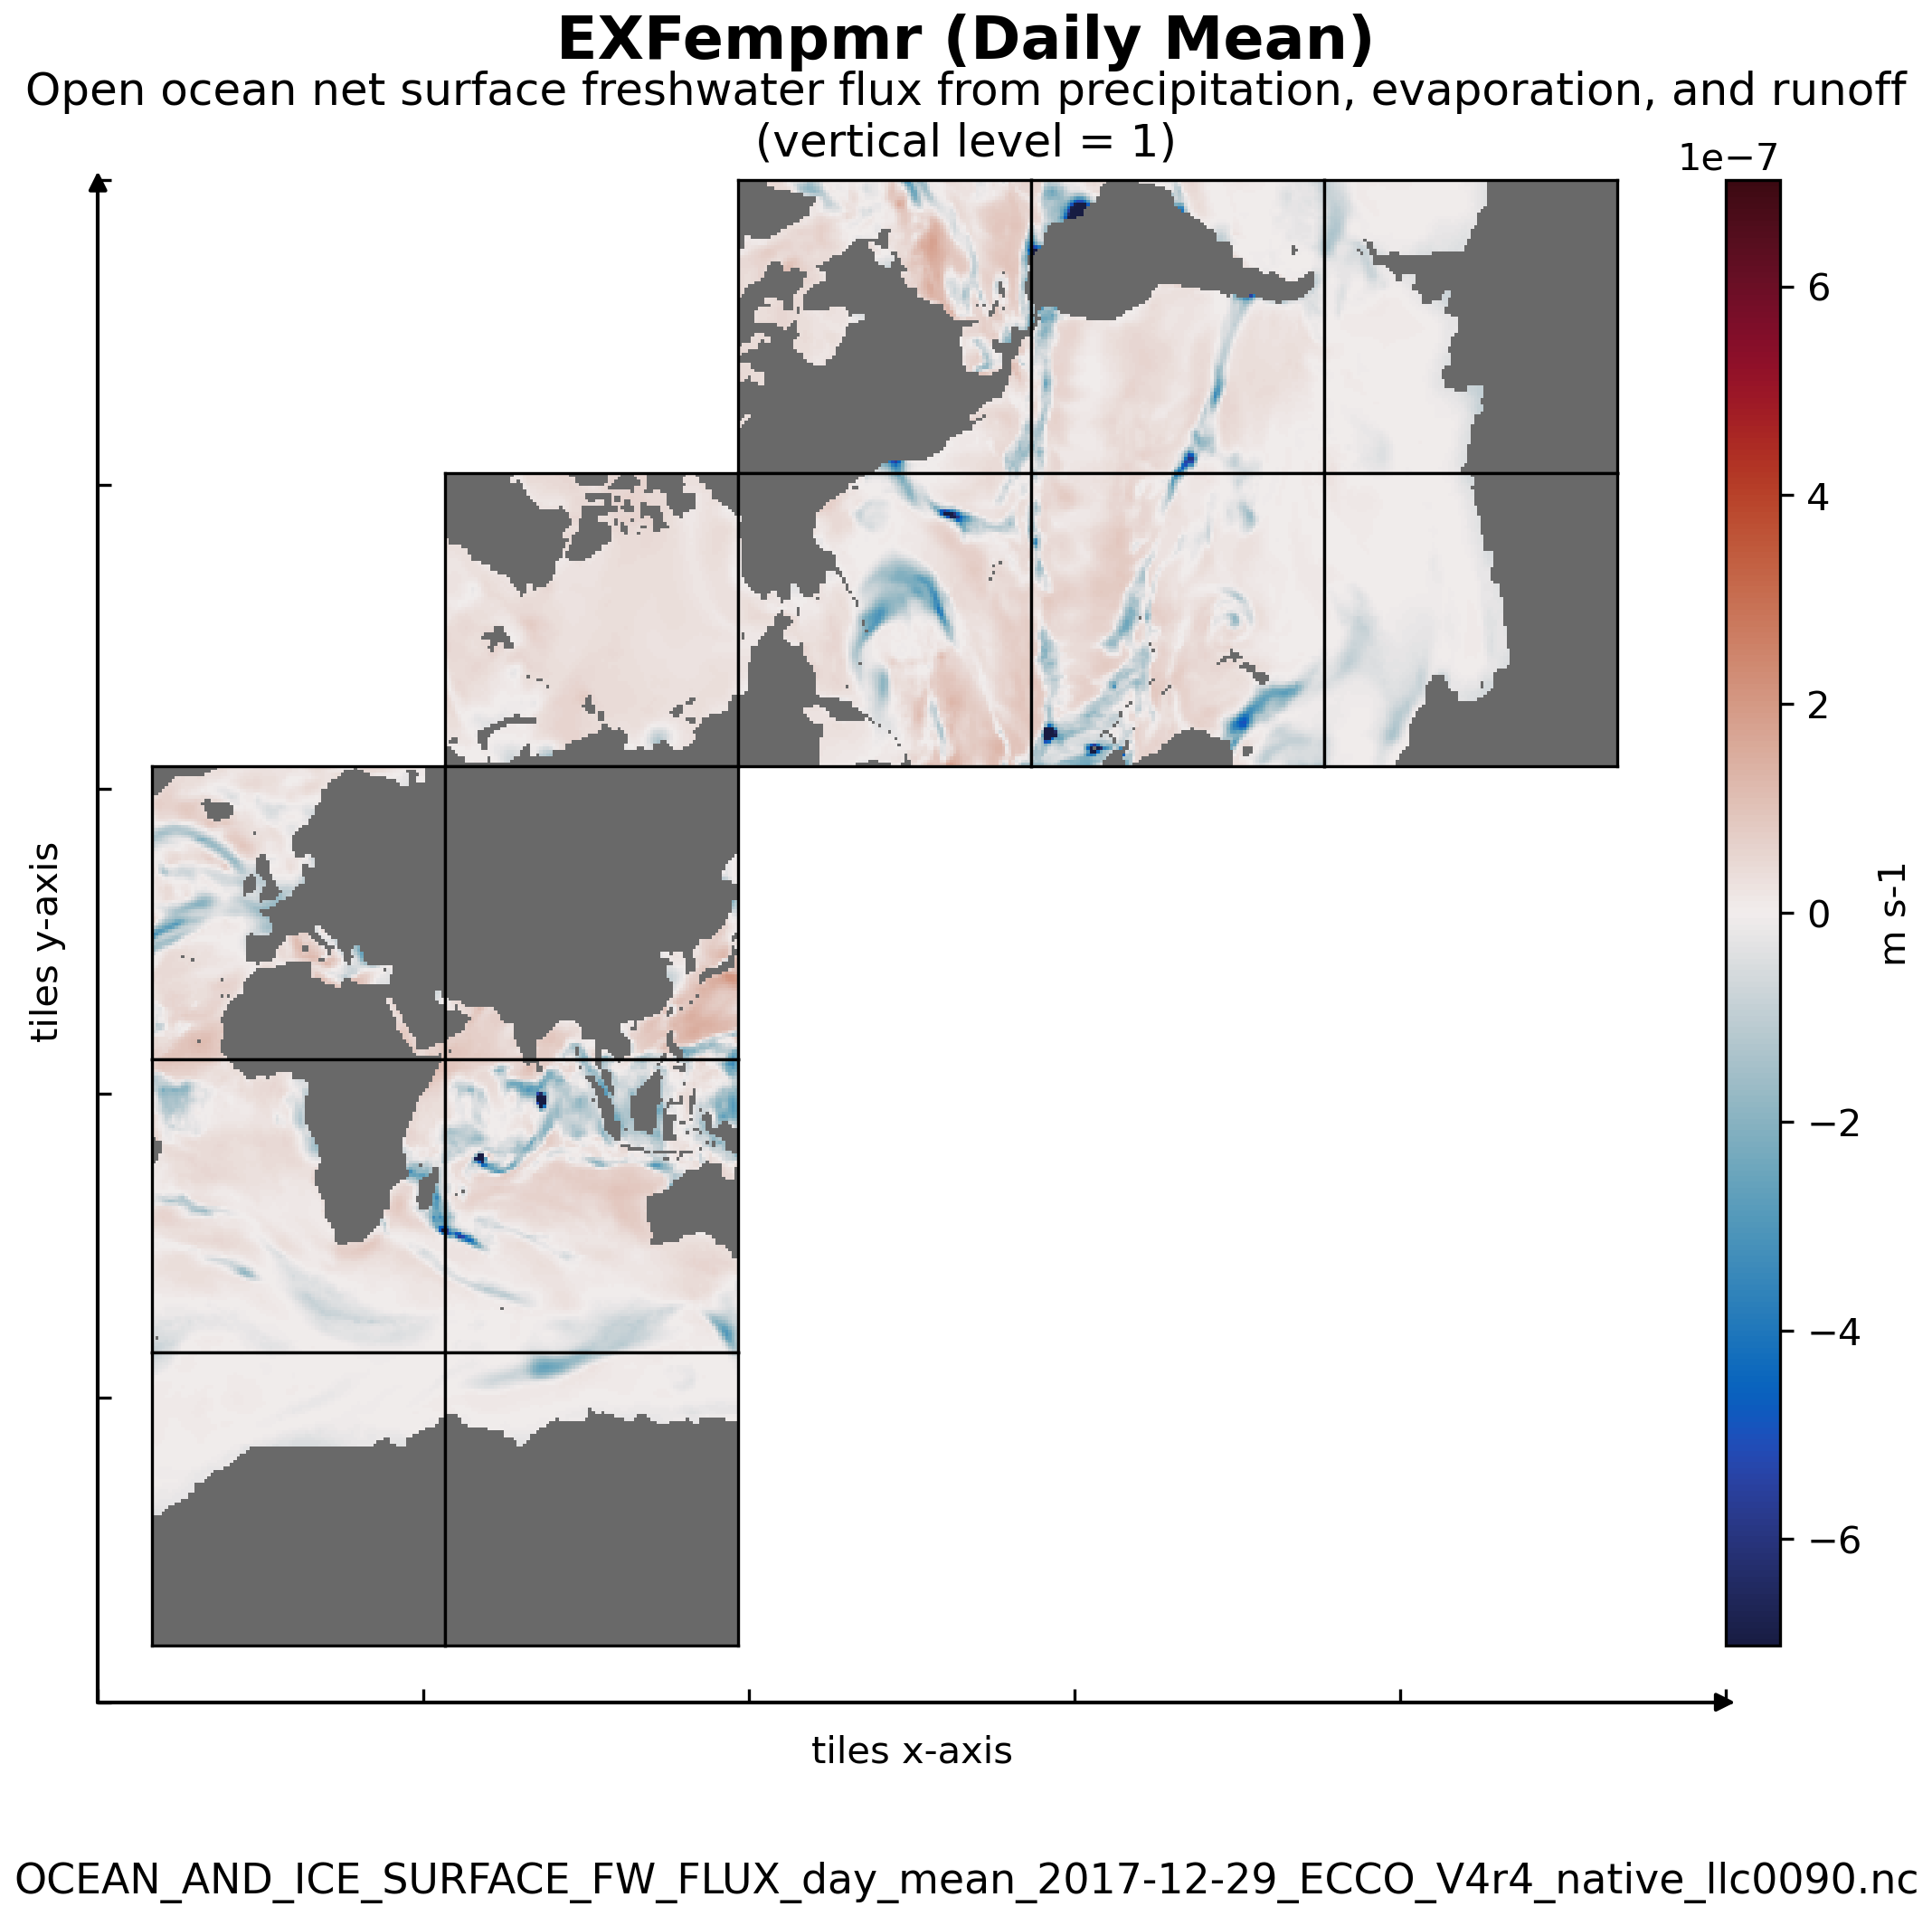
\includegraphics[scale=0.55]{../images/plots/v4r4/native_plots/Ocean_and_Sea-Ice_Surface_Freshwater_Fluxes/EXFempmr.png}
\caption{Dataset: OCEAN\_AND\_ICE\_SURFACE\_FW\_FLUX, Variable: EXFempmr}
\label{tab:table-OCEAN_AND_ICE_SURFACE_FW_FLUX_EXFempmr-Plot}
\end{figure}
\newpage
\pagebreak
\subsubsection{Native Variable: EXFevap}
\begin{longtable}{|m{0.06\textwidth}|m{0.3\textwidth}|m{0.45\textwidth}|m{0.12\textwidth}|}
\caption{Attributes description of the variable 'EXFevap' from OCEAN\_AND\_ICE\_SURFACE\_FW\_FLUX's  dataset.}
\label{tab:table-OCEAN_AND_ICE_SURFACE_FW_FLUX_EXFevap} \\ 
\hline \endhead \hline \endfoot
\rowcolor{lightgray} \textbf{Storage Type} & \textbf{Variable Name} & \textbf{Description} & \textbf{Unit} \\ \hline
float32 & EXFevap & Open ocean evaporation rate & m s-1 \\ \hline
\multicolumn{4}{|c|}{\cellcolor{lightgray}{\textbf{Description of the variable in Common Data language (CDL)}}} \\ \hline
\multicolumn{4}{|c|}{\fontfamily{lmtt}\selectfont{\makecell{\parbox{.95\textwidth}{\vspace*{0.25cm} \footnotesize{float32 EXFevap(time, tile, j, i)\\
\hspace*{0.5cm}EXFevap: \_FillValue = 9.96921e+36\\
\hspace*{0.5cm}EXFevap: coordinates = YC XC time\\
\hspace*{0.5cm}EXFevap: coverage\_content\_type = modelResult\\
\hspace*{0.5cm}EXFevap: direction = >0 increases salinity (SALT)\\
\hspace*{0.5cm}EXFevap: long\_name = Open ocean evaporation rate\\
\hspace*{0.5cm}EXFevap: standard\_name = lwe water evaporation rate\\
\hspace*{0.5cm}EXFevap: units = m s-1\\
\hspace*{0.5cm}EXFevap: valid\_max = 7.090054623404285e-07\\
\hspace*{0.5cm}EXFevap: valid\_min = -1.0958113705328287e-07\\
}}}}} \\ \hline
\rowcolor{lightgray} \multicolumn{4}{|c|}{\textbf{Comments}} \\ \hline
\multicolumn{4}{|p{1\textwidth}|}{\footnotesize{{Evaporation rate per unit area of open water (not covered by sea-ice). note: calculated using the bulk formula following large and yeager (2004) ncar/tn-460+str.}}} \\ \hline
\end{longtable}

\begin{figure}[H]
\centering
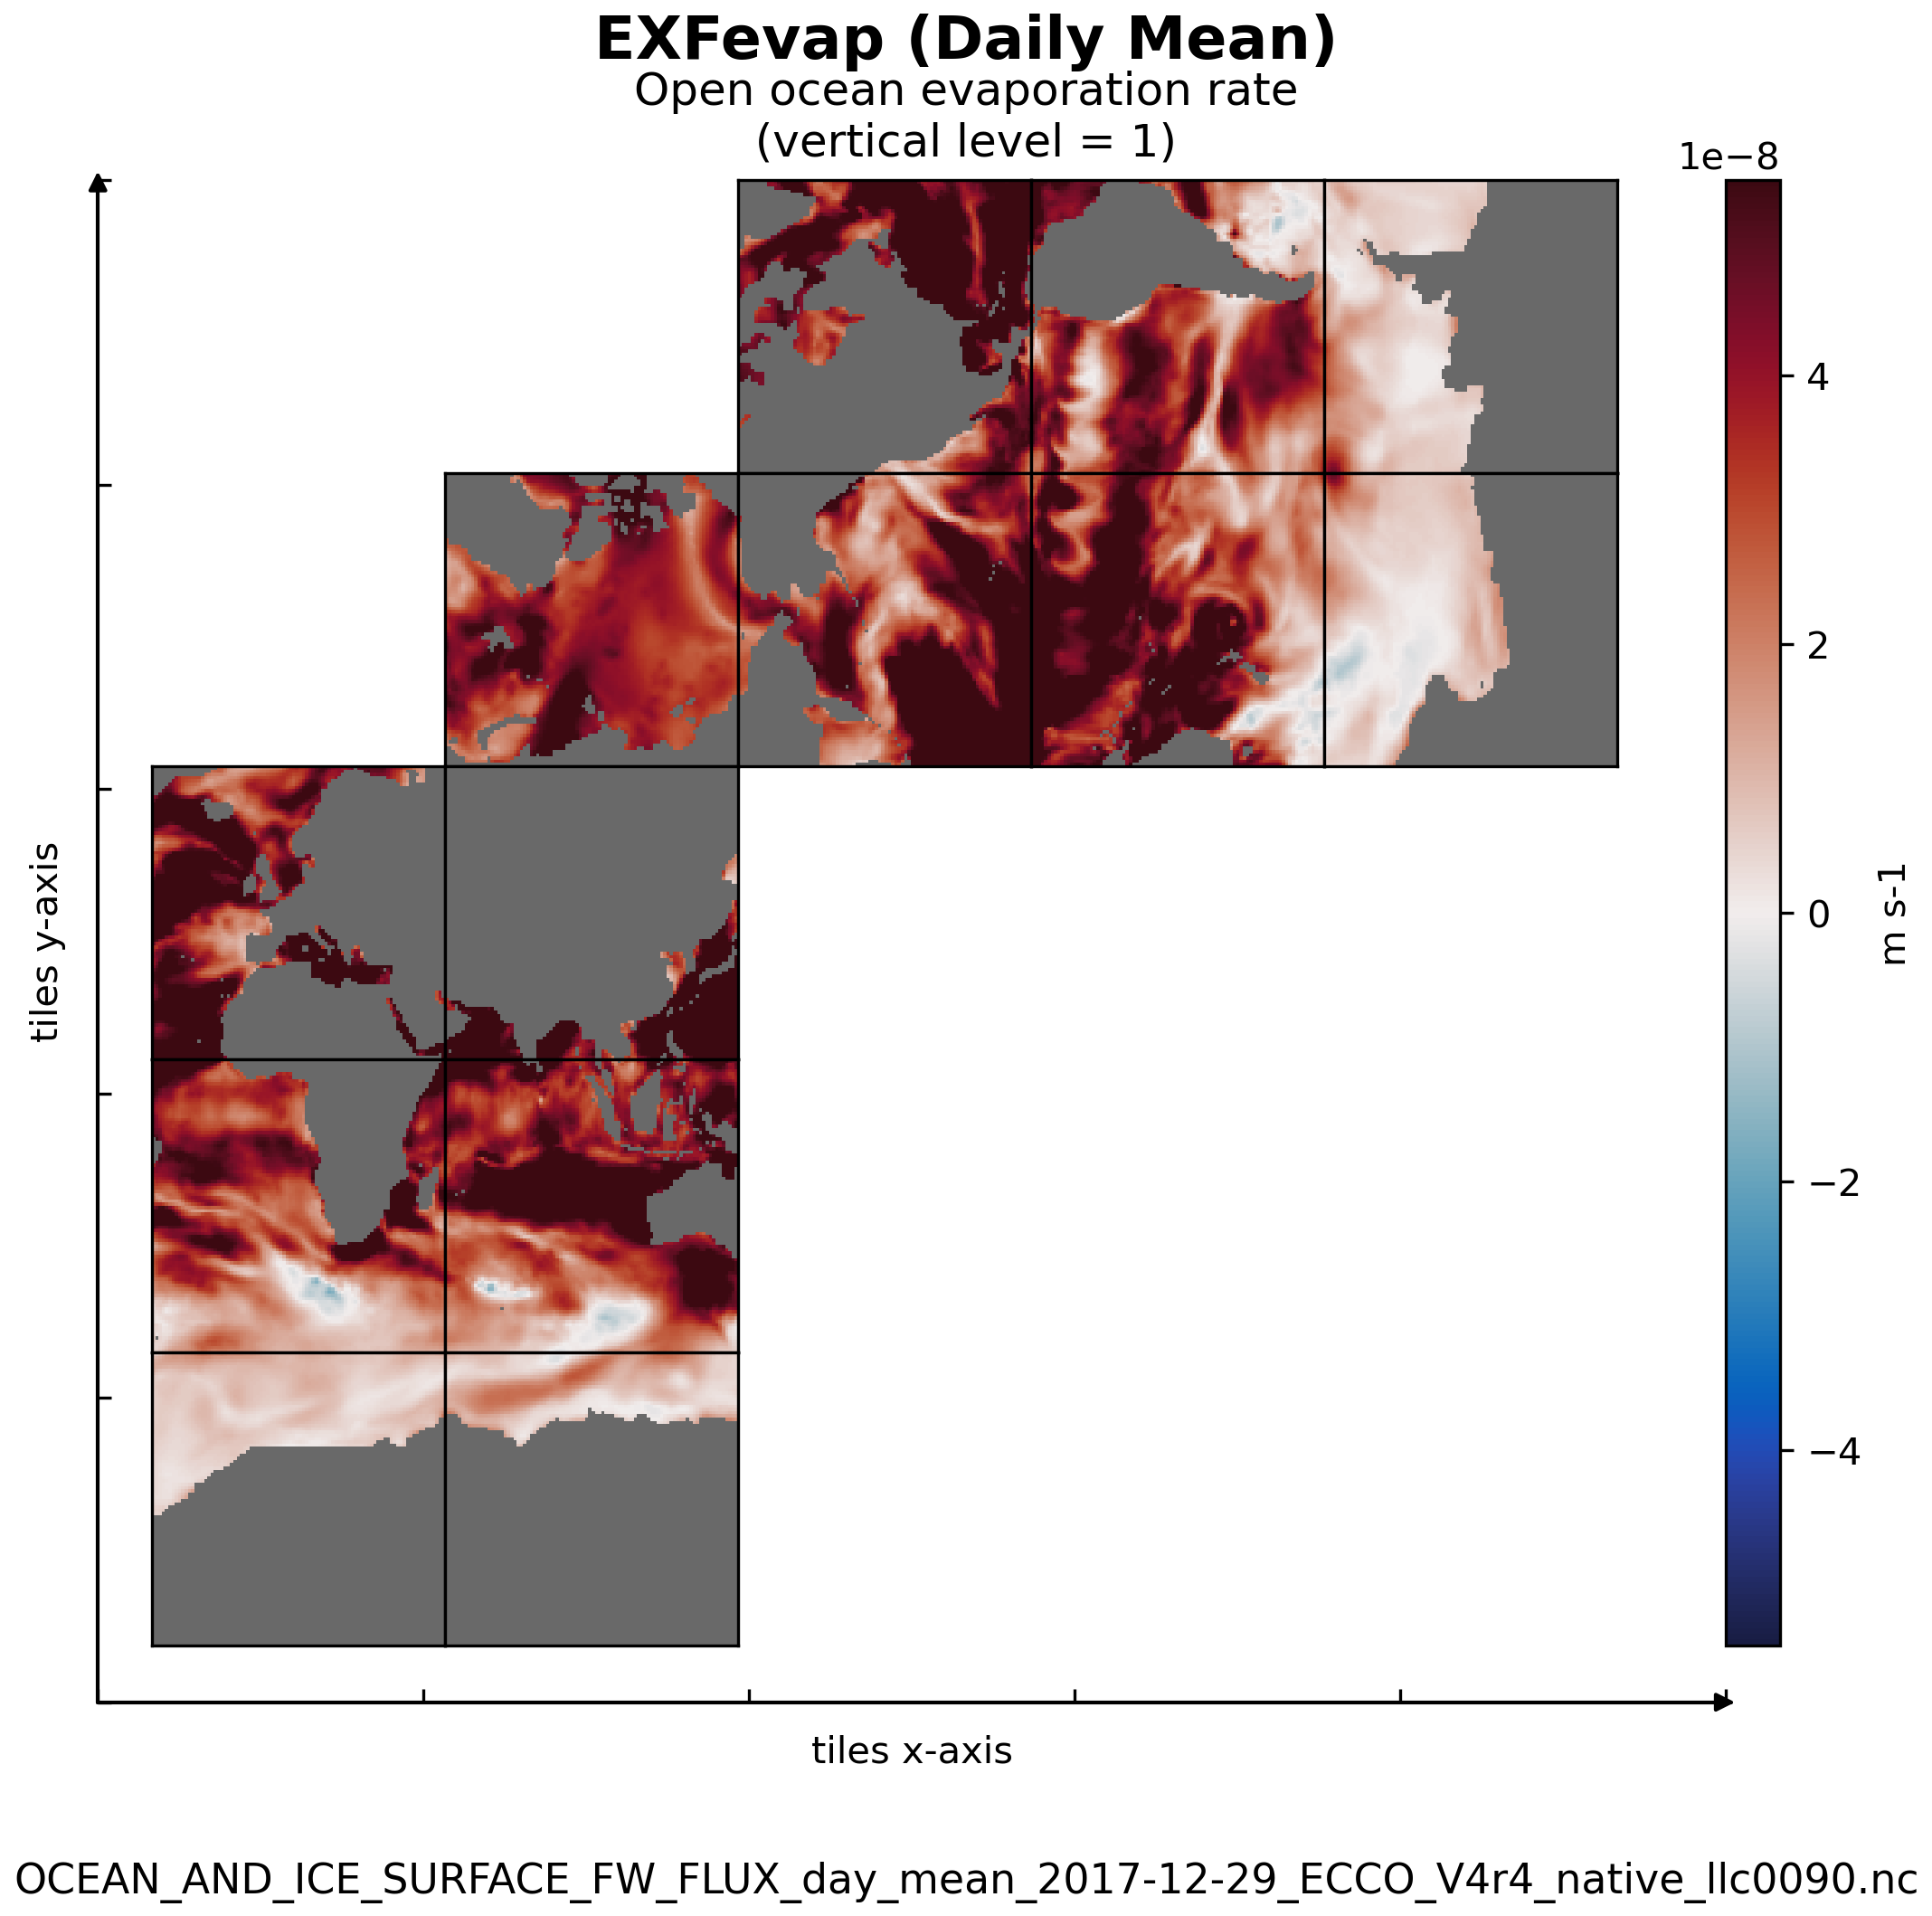
\includegraphics[scale=0.55]{../images/plots/v4r4/native_plots/Ocean_and_Sea-Ice_Surface_Freshwater_Fluxes/EXFevap.png}
\caption{Dataset: OCEAN\_AND\_ICE\_SURFACE\_FW\_FLUX, Variable: EXFevap}
\label{tab:table-OCEAN_AND_ICE_SURFACE_FW_FLUX_EXFevap-Plot}
\end{figure}
\newpage
\pagebreak
\subsubsection{Native Variable: EXFpreci}
\begin{longtable}{|m{0.06\textwidth}|m{0.3\textwidth}|m{0.45\textwidth}|m{0.12\textwidth}|}
\caption{Attributes description of the variable 'EXFpreci' from OCEAN\_AND\_ICE\_SURFACE\_FW\_FLUX's  dataset.}
\label{tab:table-OCEAN_AND_ICE_SURFACE_FW_FLUX_EXFpreci} \\ 
\hline \endhead \hline \endfoot
\rowcolor{lightgray} \textbf{Storage Type} & \textbf{Variable Name} & \textbf{Description} & \textbf{Unit} \\ \hline
float32 & EXFpreci & Precipitation rate & m s-1 \\ \hline
\multicolumn{4}{|c|}{\cellcolor{lightgray}{\textbf{Description of the variable in Common Data language (CDL)}}} \\ \hline
\multicolumn{4}{|c|}{\fontfamily{lmtt}\selectfont{\makecell{\parbox{.95\textwidth}{\vspace*{0.25cm} \footnotesize{float32 EXFpreci(time, tile, j, i)\\
\hspace*{0.5cm}EXFpreci: \_FillValue = 9.96921e+36\\
\hspace*{0.5cm}EXFpreci: coordinates = YC XC time\\
\hspace*{0.5cm}EXFpreci: coverage\_content\_type = modelResult\\
\hspace*{0.5cm}EXFpreci: direction = >0 increases salinity (SALT)\\
\hspace*{0.5cm}EXFpreci: long\_name = Precipitation rate\\
\hspace*{0.5cm}EXFpreci: standard\_name = lwe precipitation rate\\
\hspace*{0.5cm}EXFpreci: units = m s-1\\
\hspace*{0.5cm}EXFpreci: valid\_max = 8.317776519106701e-06\\
\hspace*{0.5cm}EXFpreci: valid\_min = -1.4860395936011628e-07\\
}}}}} \\ \hline
\rowcolor{lightgray} \multicolumn{4}{|c|}{\textbf{Comments}} \\ \hline
\multicolumn{4}{|p{1\textwidth}|}{\footnotesize{{Precipitation rate. note: sum of era-interim precipitation and the control adjustment from ocean state estimation.}}} \\ \hline
\end{longtable}

\begin{figure}[H]
\centering
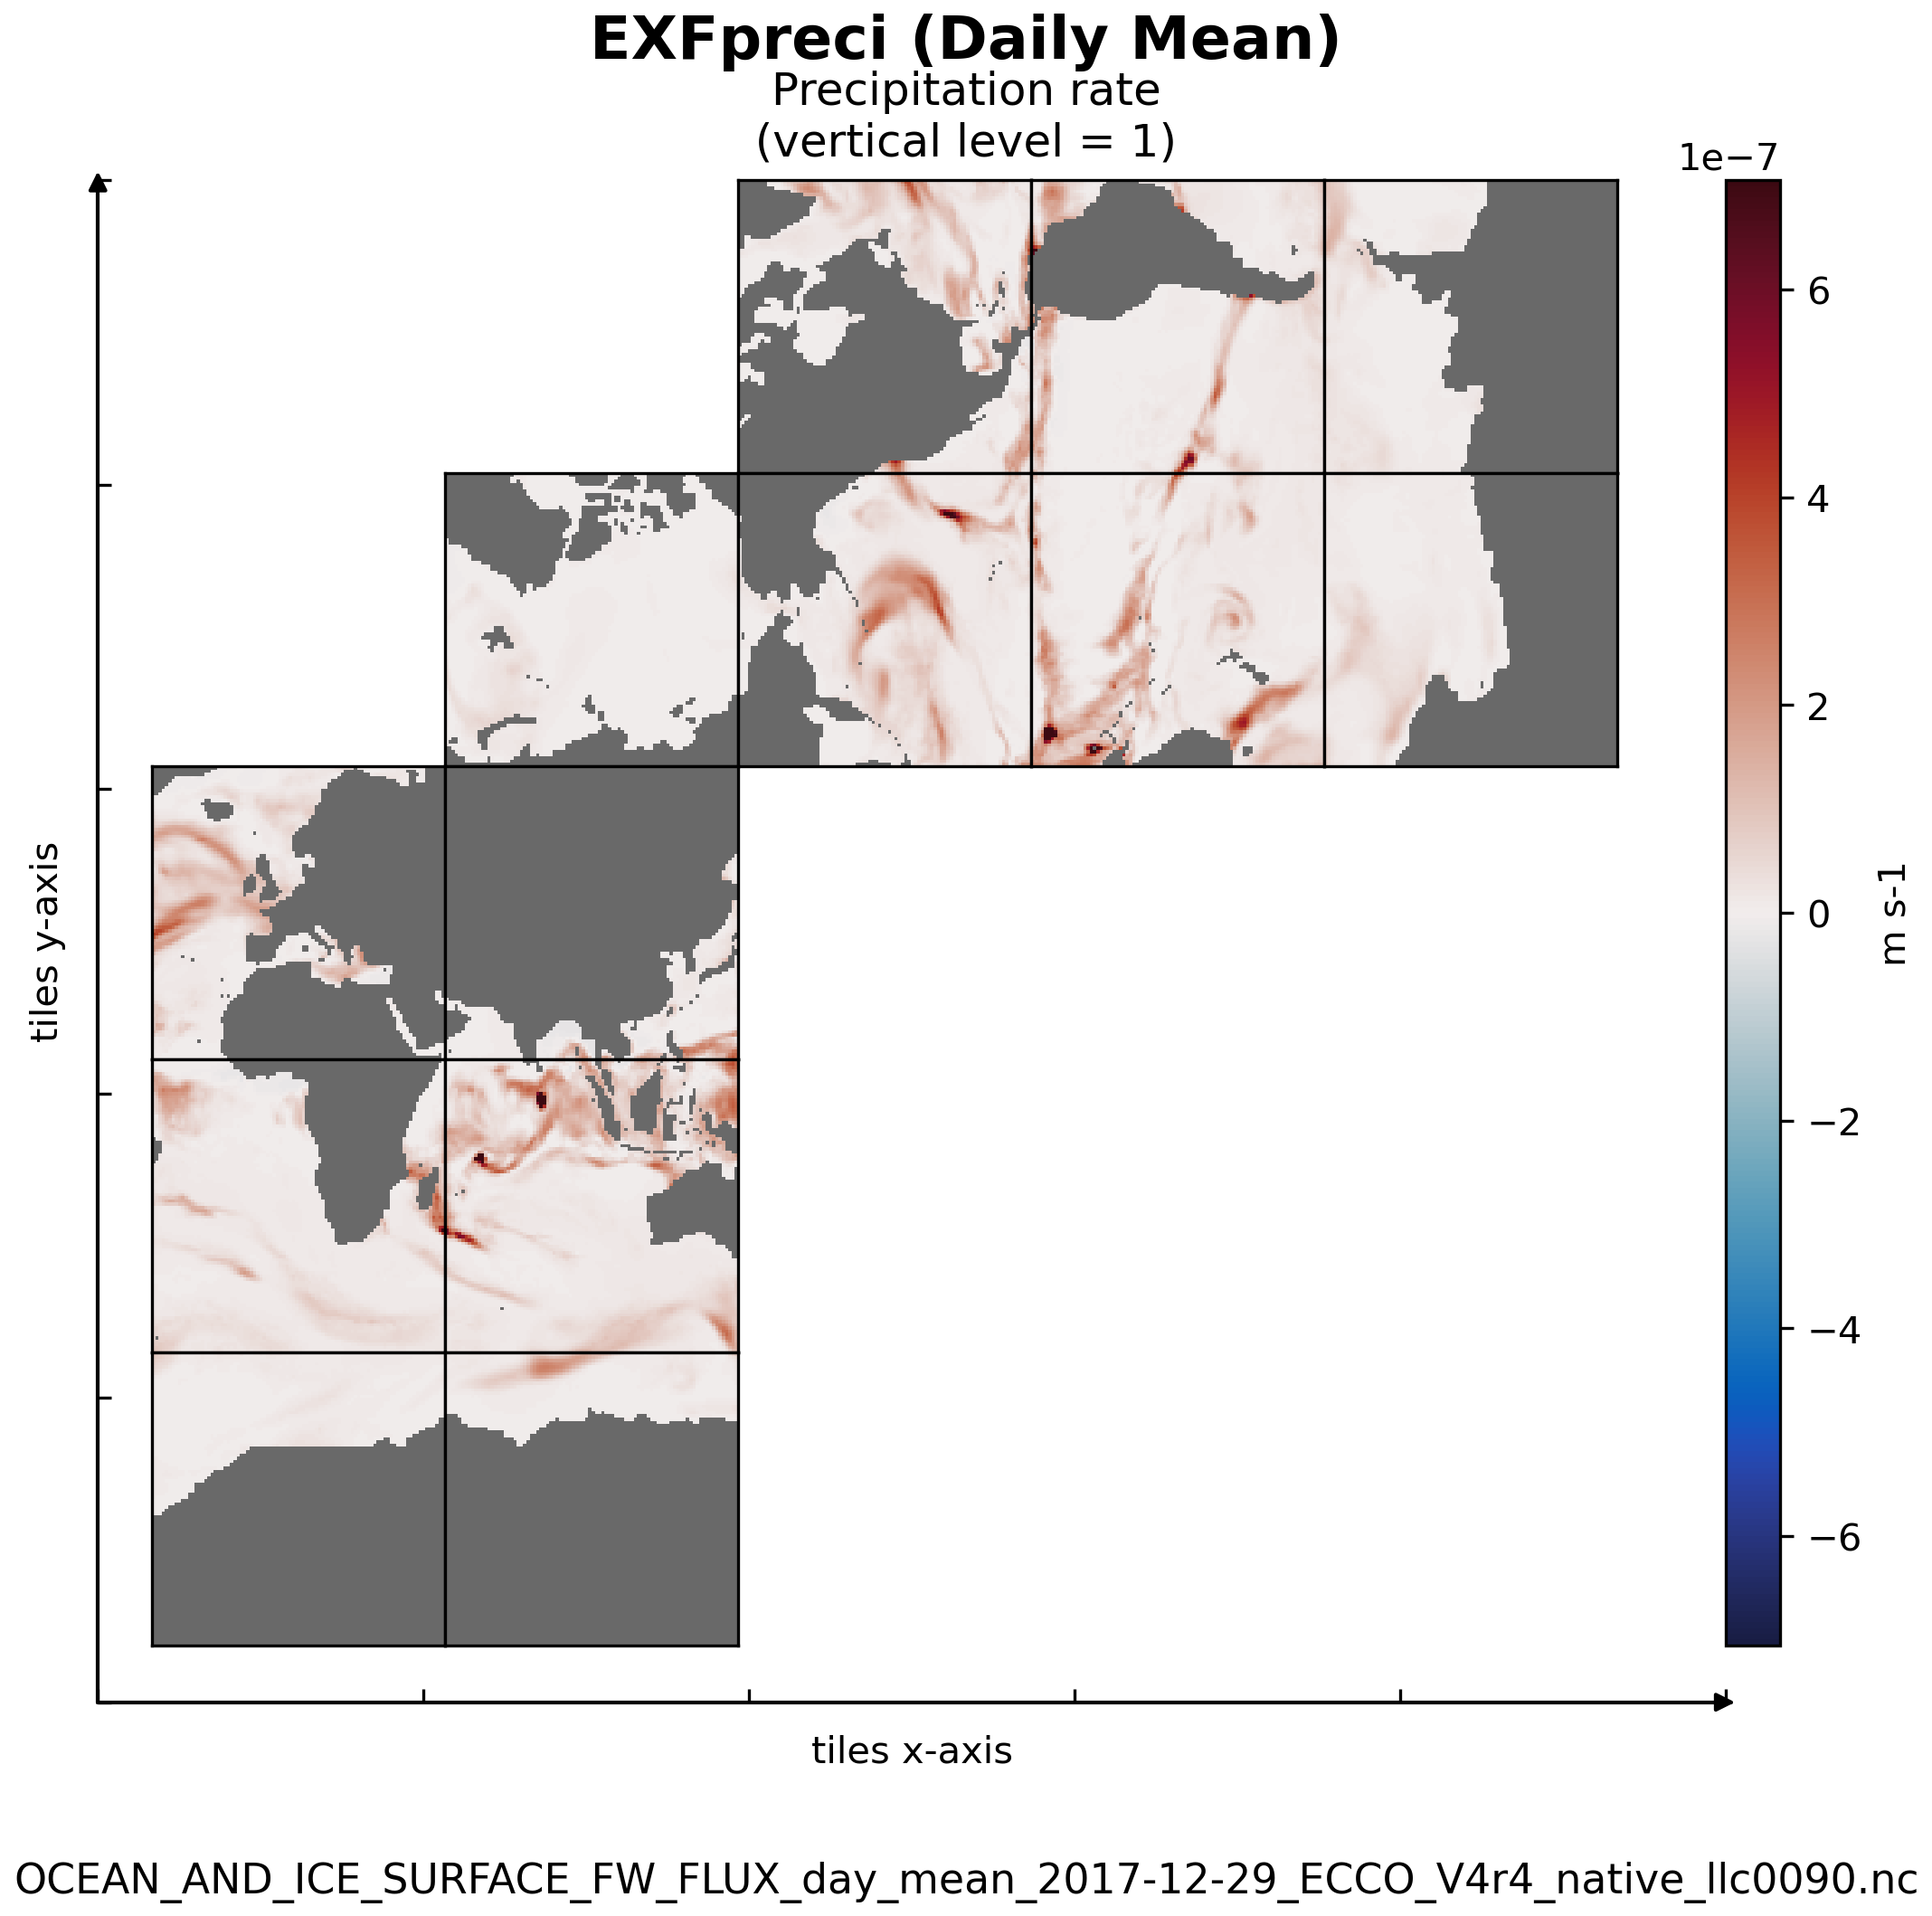
\includegraphics[scale=0.55]{../images/plots/v4r4/native_plots/Ocean_and_Sea-Ice_Surface_Freshwater_Fluxes/EXFpreci.png}
\caption{Dataset: OCEAN\_AND\_ICE\_SURFACE\_FW\_FLUX, Variable: EXFpreci}
\label{tab:table-OCEAN_AND_ICE_SURFACE_FW_FLUX_EXFpreci-Plot}
\end{figure}
\newpage
\pagebreak
\subsubsection{Native Variable: EXFroff}
\begin{longtable}{|m{0.06\textwidth}|m{0.3\textwidth}|m{0.45\textwidth}|m{0.12\textwidth}|}
\caption{Attributes description of the variable 'EXFroff' from OCEAN\_AND\_ICE\_SURFACE\_FW\_FLUX's  dataset.}
\label{tab:table-OCEAN_AND_ICE_SURFACE_FW_FLUX_EXFroff} \\ 
\hline \endhead \hline \endfoot
\rowcolor{lightgray} \textbf{Storage Type} & \textbf{Variable Name} & \textbf{Description} & \textbf{Unit} \\ \hline
float32 & EXFroff & River runoff & m s-1 \\ \hline
\multicolumn{4}{|c|}{\cellcolor{lightgray}{\textbf{Description of the variable in Common Data language (CDL)}}} \\ \hline
\multicolumn{4}{|c|}{\fontfamily{lmtt}\selectfont{\makecell{\parbox{.95\textwidth}{\vspace*{0.25cm} \footnotesize{float32 EXFroff(time, tile, j, i)\\
\hspace*{0.5cm}EXFroff: \_FillValue = 9.96921e+36\\
\hspace*{0.5cm}EXFroff: coordinates = YC XC time\\
\hspace*{0.5cm}EXFroff: coverage\_content\_type = modelResult\\
\hspace*{0.5cm}EXFroff: direction = >0 increases salinity (SALT)\\
\hspace*{0.5cm}EXFroff: long\_name = River runoff\\
\hspace*{0.5cm}EXFroff: standard\_name = surface runoff flux\\
\hspace*{0.5cm}EXFroff: units = m s-1\\
\hspace*{0.5cm}EXFroff: valid\_max = 4.185612397122895e-06\\
\hspace*{0.5cm}EXFroff: valid\_min = 0.0\\
}}}}} \\ \hline
\rowcolor{lightgray} \multicolumn{4}{|c|}{\textbf{Comments}} \\ \hline
\multicolumn{4}{|p{1\textwidth}|}{\footnotesize{{River runoff freshwater flux. note: not adjusted by the optimization.}}} \\ \hline
\end{longtable}

\begin{figure}[H]
\centering
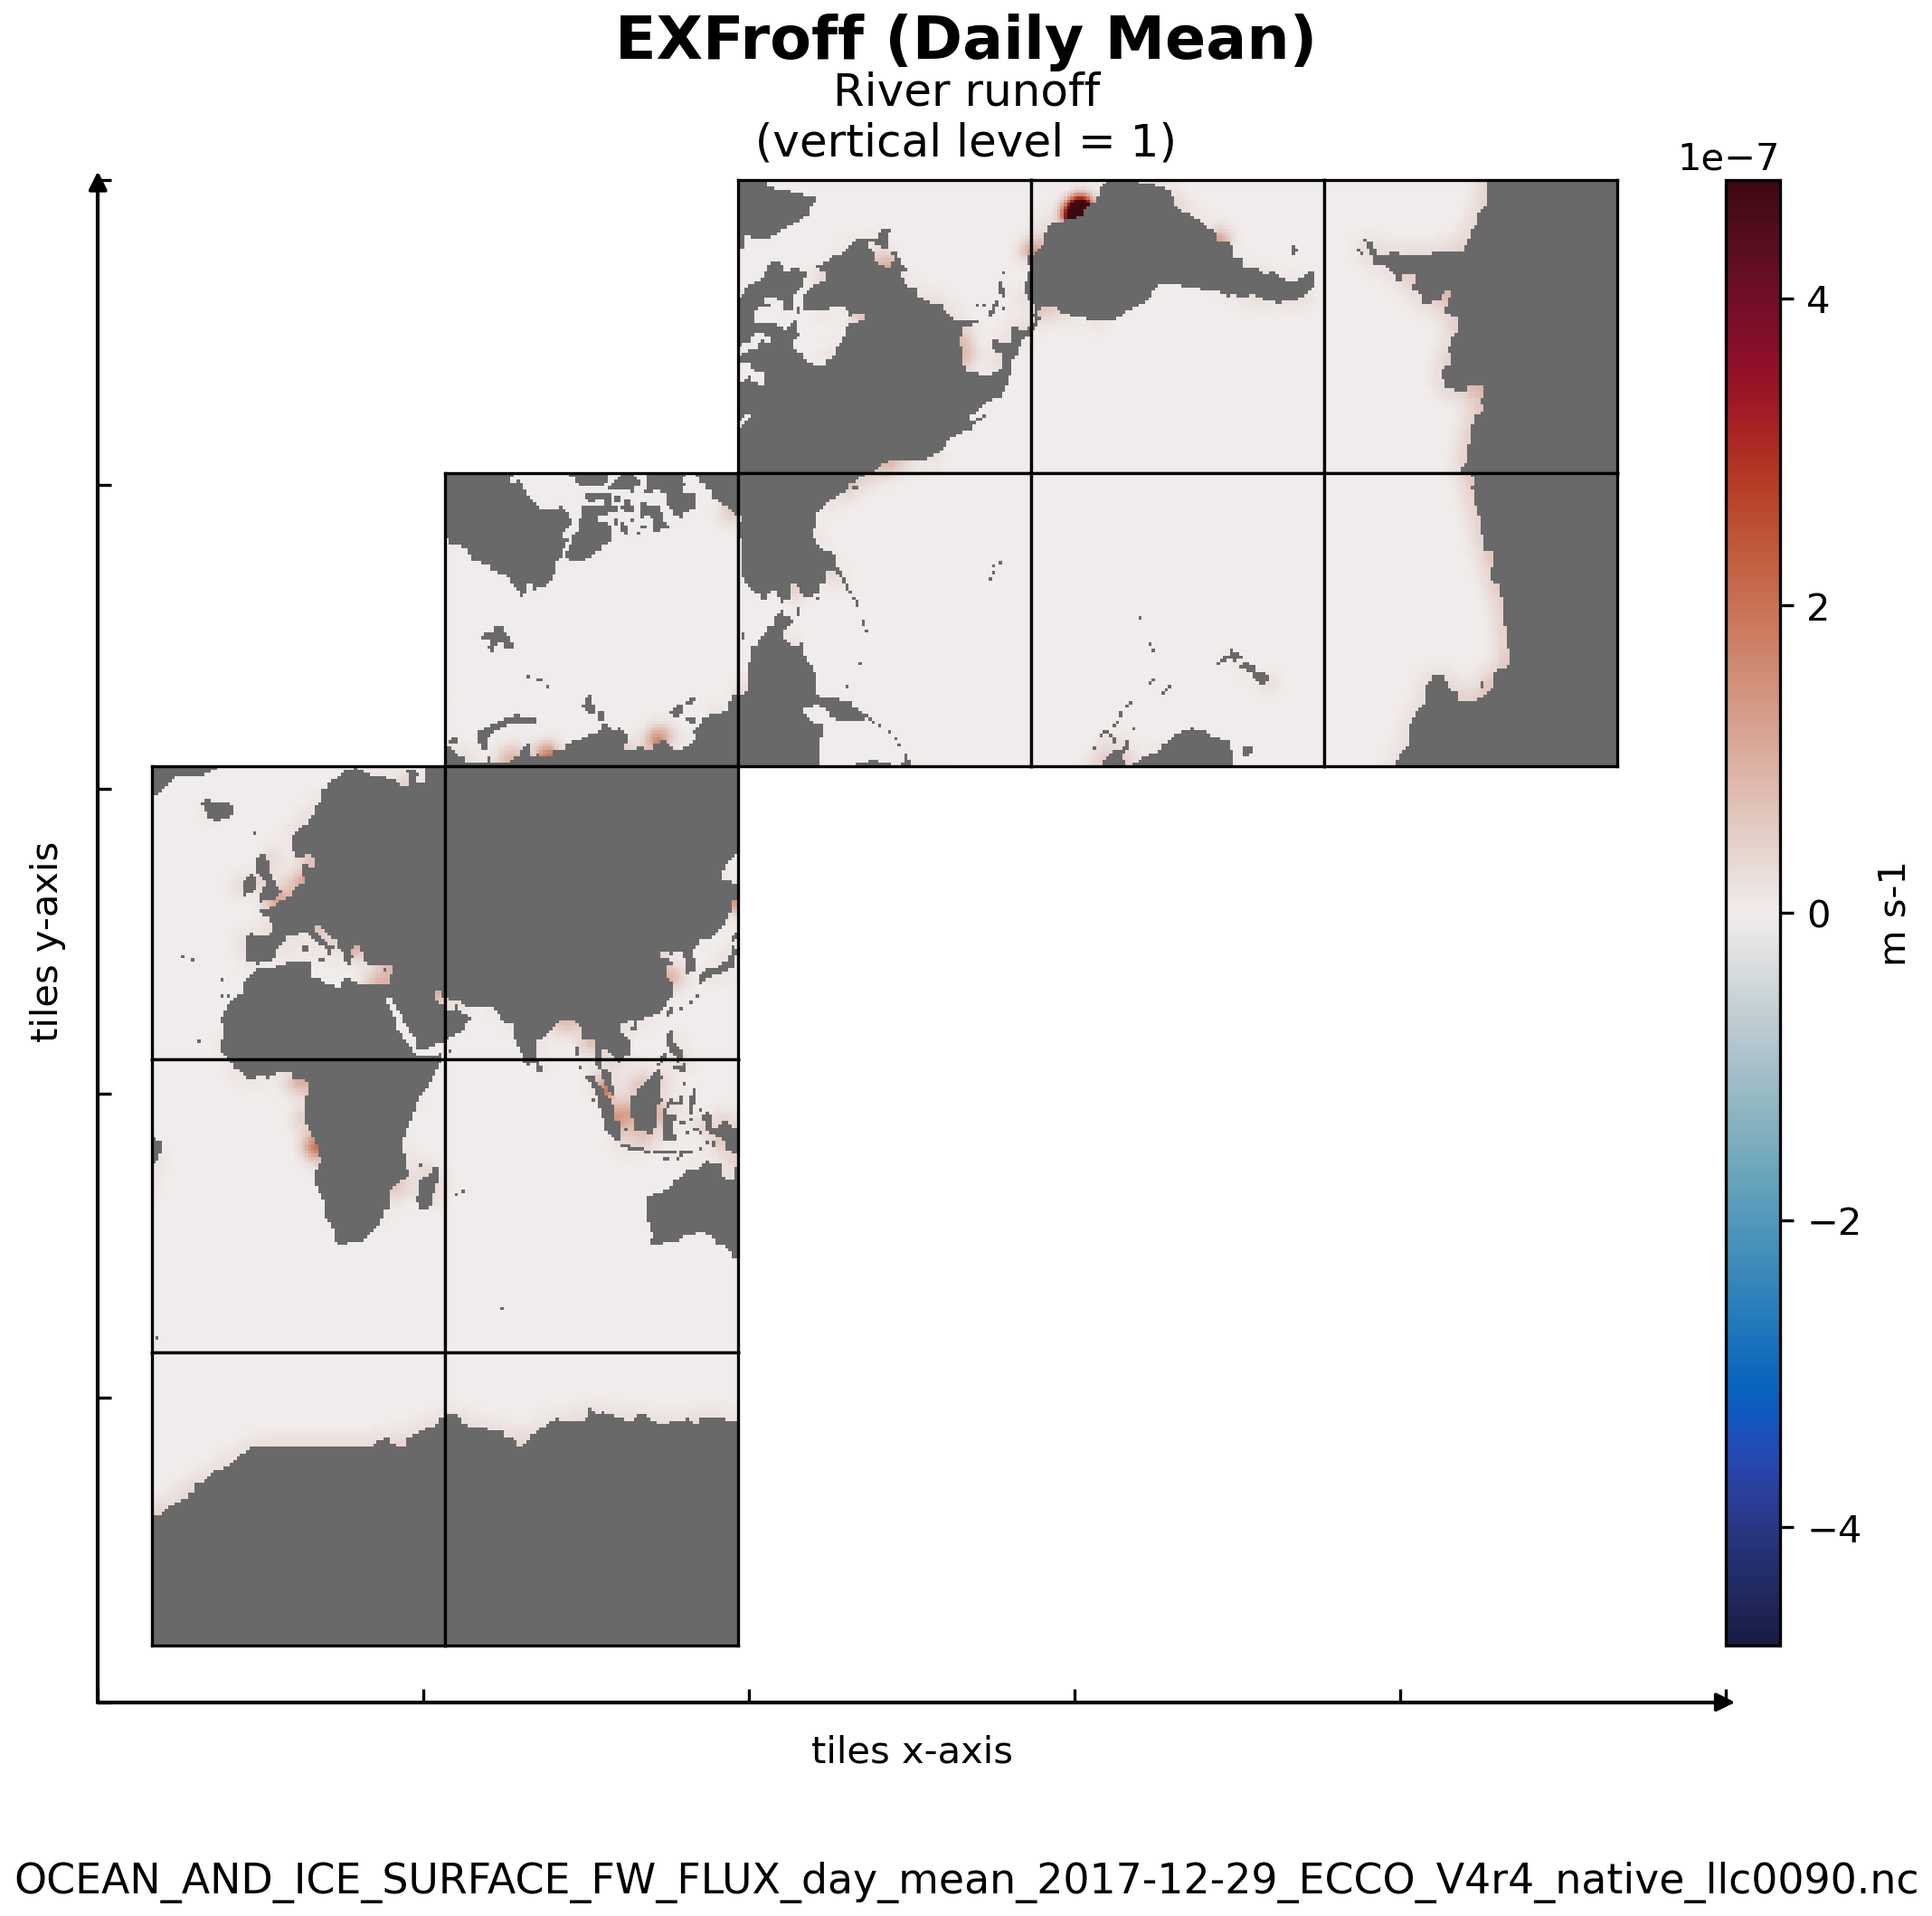
\includegraphics[scale=0.55]{../images/plots/v4r4/native_plots/Ocean_and_Sea-Ice_Surface_Freshwater_Fluxes/EXFroff.png}
\caption{Dataset: OCEAN\_AND\_ICE\_SURFACE\_FW\_FLUX, Variable: EXFroff}
\label{tab:table-OCEAN_AND_ICE_SURFACE_FW_FLUX_EXFroff-Plot}
\end{figure}
\newpage
\pagebreak
\subsubsection{Native Variable: SFLUX}
\begin{longtable}{|m{0.06\textwidth}|m{0.3\textwidth}|m{0.45\textwidth}|m{0.12\textwidth}|}
\caption{Attributes description of the variable 'SFLUX' from OCEAN\_AND\_ICE\_SURFACE\_FW\_FLUX's  dataset.}
\label{tab:table-OCEAN_AND_ICE_SURFACE_FW_FLUX_SFLUX} \\ 
\hline \endhead \hline \endfoot
\rowcolor{lightgray} \textbf{Storage Type} & \textbf{Variable Name} & \textbf{Description} & \textbf{Unit} \\ \hline
float32 & SFLUX & Rate of change of total ocean salinity per m2 accounting for mass fluxes. & g m-2 s-1 \\ \hline
\multicolumn{4}{|c|}{\cellcolor{lightgray}{\textbf{Description of the variable in Common Data language (CDL)}}} \\ \hline
\multicolumn{4}{|c|}{\fontfamily{lmtt}\selectfont{\makecell{\parbox{.95\textwidth}{\vspace*{0.25cm} \footnotesize{float32 SFLUX(time, tile, j, i)\\
\hspace*{0.5cm}SFLUX: \_FillValue = 9.96921e+36\\
\hspace*{0.5cm}SFLUX: coordinates = YC XC time\\
\hspace*{0.5cm}SFLUX: coverage\_content\_type = modelResult\\
\hspace*{0.5cm}SFLUX: direction = >0 increases salinity (SALT)\\
\hspace*{0.5cm}SFLUX: long\_name = Rate of change of total ocean salinity per m2 accounting for mass fluxes.\\
\hspace*{0.5cm}SFLUX: units = g m-2 s-1\\
\hspace*{0.5cm}SFLUX: valid\_max = 0.010607733391225338\\
\hspace*{0.5cm}SFLUX: valid\_min = -0.07353577762842178\\
}}}}} \\ \hline
\rowcolor{lightgray} \multicolumn{4}{|c|}{\textbf{Comments}} \\ \hline
\multicolumn{4}{|p{1\textwidth}|}{\footnotesize{{The rate of change of total ocean salinity due to freshwater fluxes across the liquid surface and the addition or removal of mass. note: the global area integral of sflux matches the time-derivative of total ocean salinity (psu s-1). unlike ocefwflx, sflux includes the contribution to the total ocean salinity from changing ocean mass (e.g. from the addition or removal of freshwater in ocefwflx). }}} \\ \hline
\end{longtable}

\begin{figure}[H]
\centering
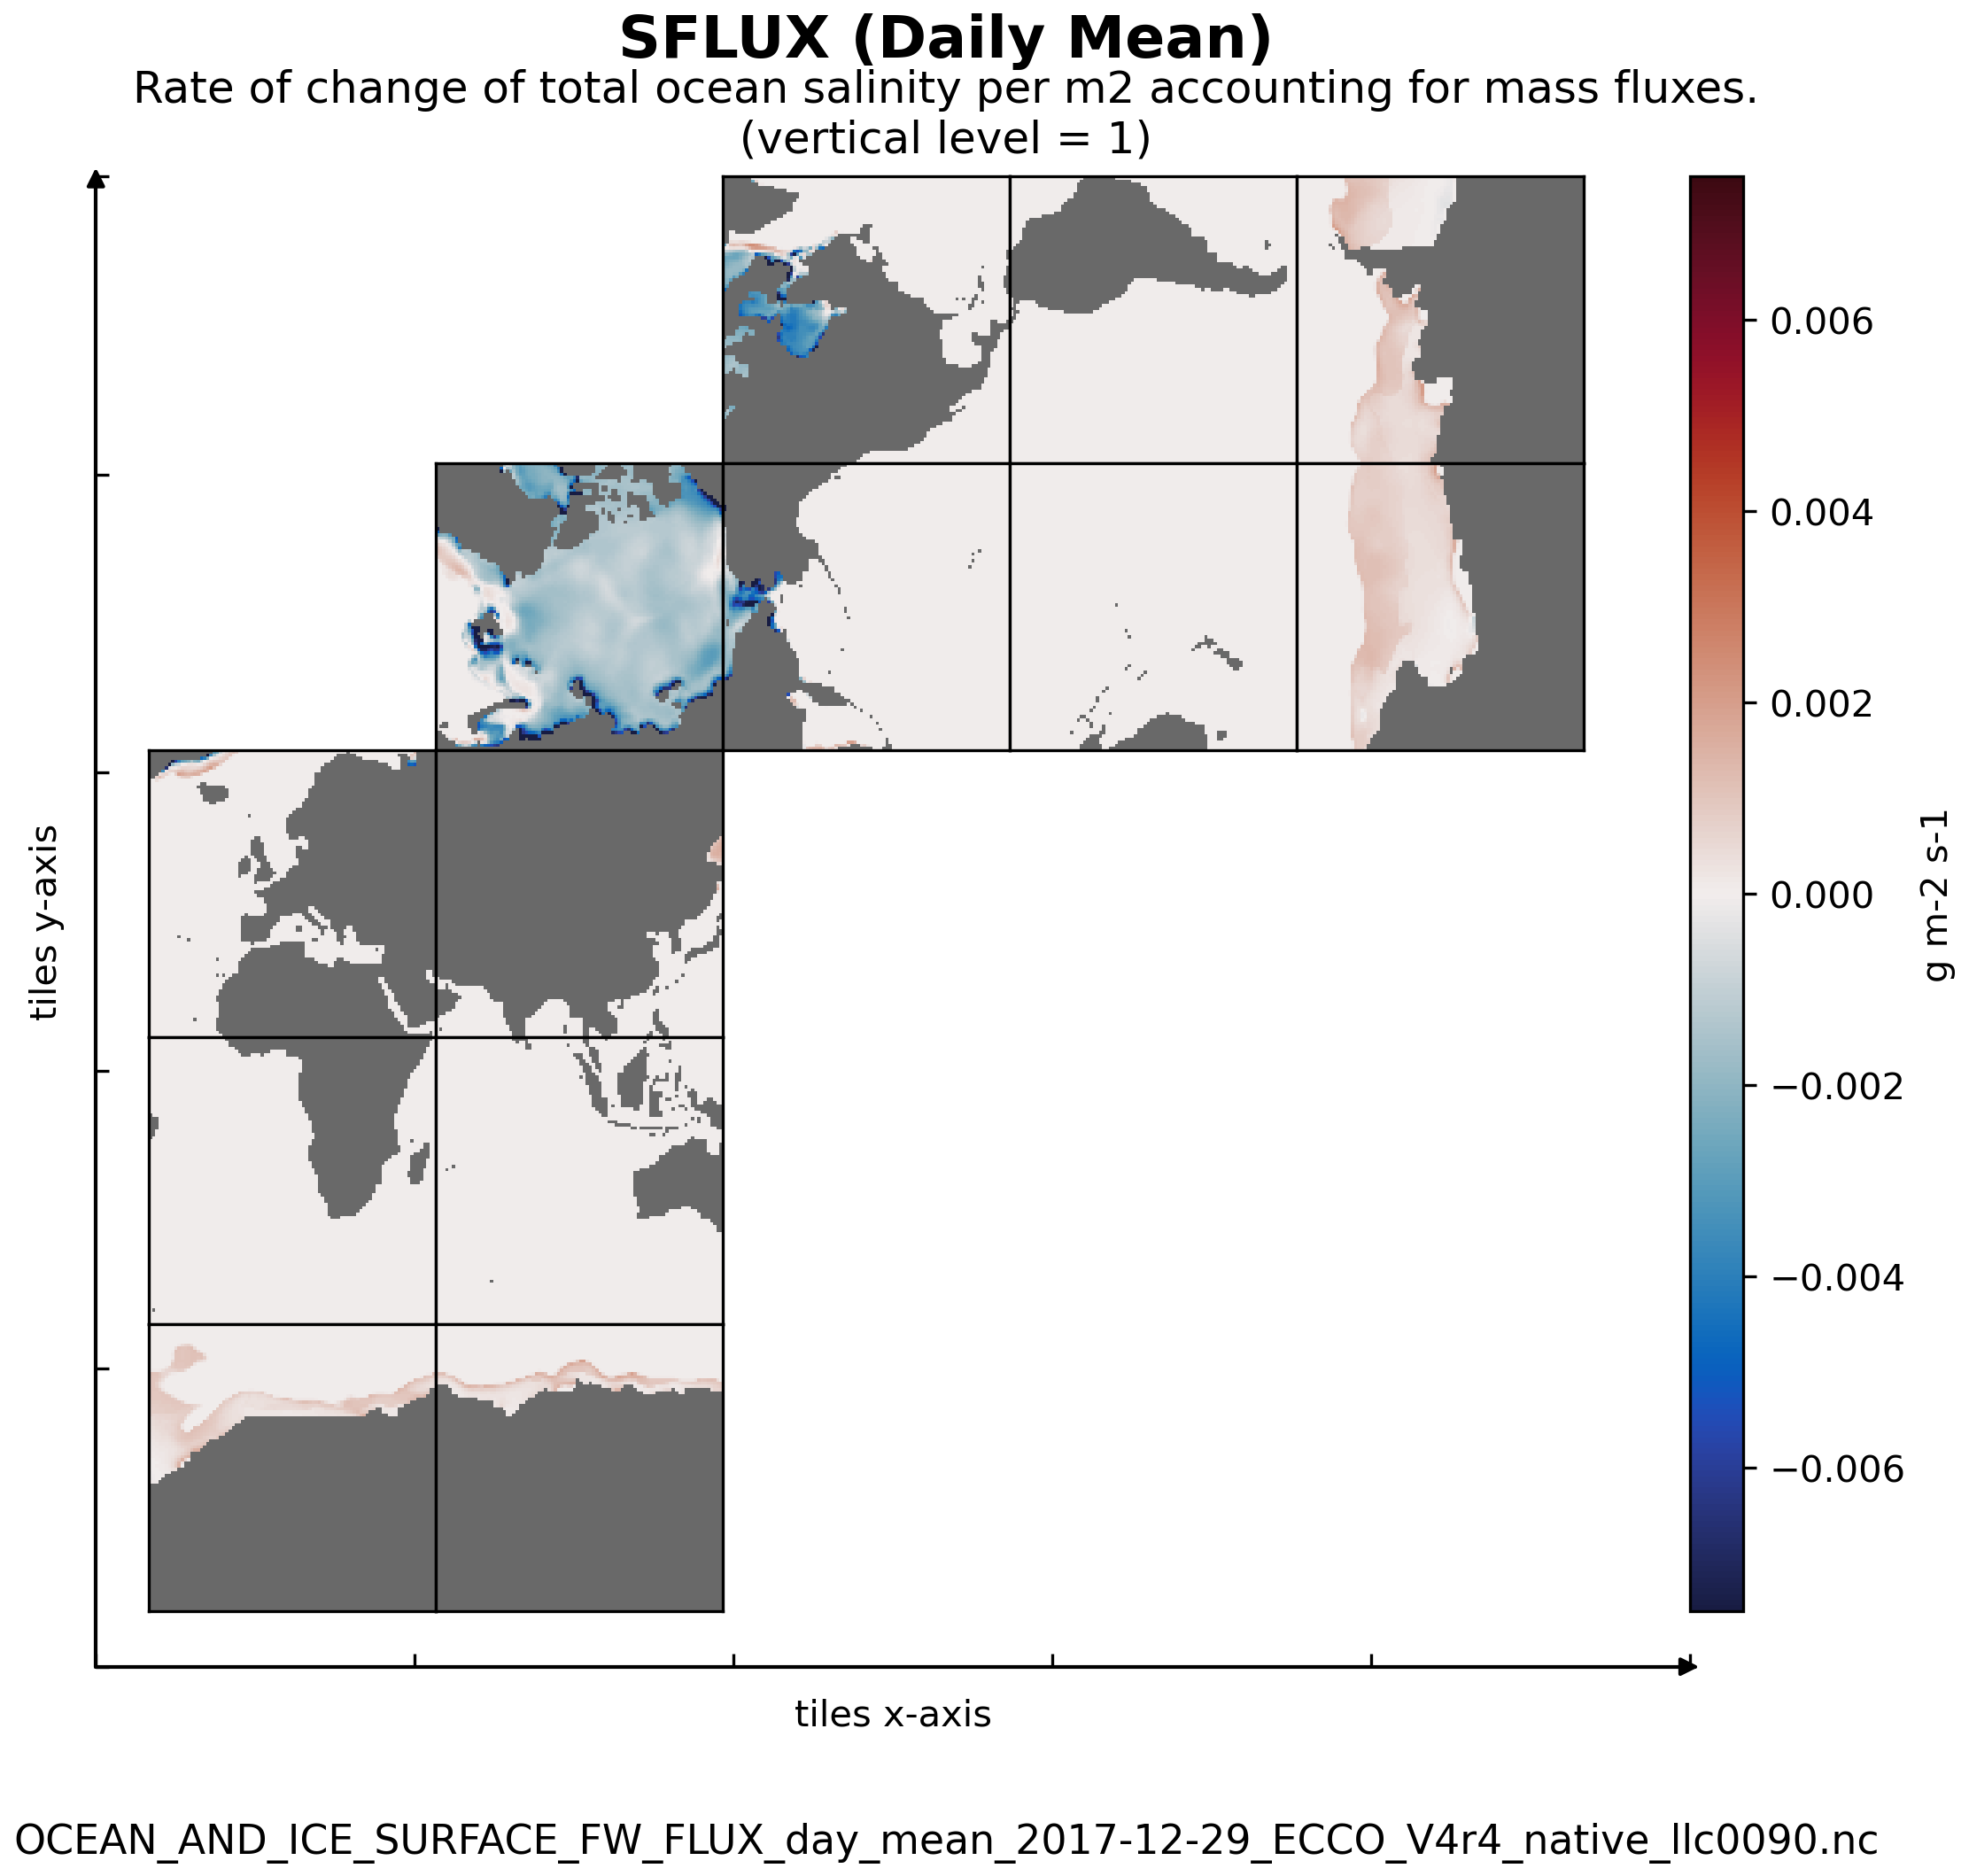
\includegraphics[scale=0.55]{../images/plots/v4r4/native_plots/Ocean_and_Sea-Ice_Surface_Freshwater_Fluxes/SFLUX.png}
\caption{Dataset: OCEAN\_AND\_ICE\_SURFACE\_FW\_FLUX, Variable: SFLUX}
\label{tab:table-OCEAN_AND_ICE_SURFACE_FW_FLUX_SFLUX-Plot}
\end{figure}
\newpage
\pagebreak
\subsubsection{Native Variable: SIacSubl}
\begin{longtable}{|m{0.06\textwidth}|m{0.3\textwidth}|m{0.45\textwidth}|m{0.12\textwidth}|}
\caption{Attributes description of the variable 'SIacSubl' from OCEAN\_AND\_ICE\_SURFACE\_FW\_FLUX's  dataset.}
\label{tab:table-OCEAN_AND_ICE_SURFACE_FW_FLUX_SIacSubl} \\ 
\hline \endhead \hline \endfoot
\rowcolor{lightgray} \textbf{Storage Type} & \textbf{Variable Name} & \textbf{Description} & \textbf{Unit} \\ \hline
float32 & SIacSubl & Freshwater flux to the atmosphere due to sublimation-deposition of snow or ice & kg m-2 s-1 \\ \hline
\multicolumn{4}{|c|}{\cellcolor{lightgray}{\textbf{Description of the variable in Common Data language (CDL)}}} \\ \hline
\multicolumn{4}{|c|}{\fontfamily{lmtt}\selectfont{\makecell{\parbox{.95\textwidth}{\vspace*{0.25cm} \footnotesize{float32 SIacSubl(time, tile, j, i)\\
\hspace*{0.5cm}SIacSubl: \_FillValue = 9.96921e+36\\
\hspace*{0.5cm}SIacSubl: coordinates = YC XC time\\
\hspace*{0.5cm}SIacSubl: coverage\_content\_type = modelResult\\
\hspace*{0.5cm}SIacSubl: direction = >0 decreases snow or sea-ice thickness (HSNOW or HEFF)\\
\hspace*{0.5cm}SIacSubl: long\_name = Freshwater flux to the atmosphere due to sublimation-deposition of snow or ice\\
\hspace*{0.5cm}SIacSubl: standard\_name = water sublimation flux\\
\hspace*{0.5cm}SIacSubl: units = kg m-2 s-1\\
\hspace*{0.5cm}SIacSubl: valid\_max = 8.154580427799374e-05\\
\hspace*{0.5cm}SIacSubl: valid\_min = 0.0\\
}}}}} \\ \hline
\rowcolor{lightgray} \multicolumn{4}{|c|}{\textbf{Comments}} \\ \hline
\multicolumn{4}{|p{1\textwidth}|}{\footnotesize{{Freshwater flux to the atmosphere due to sublimation-deposition of snow or ice. positive values imply sublimation from ice/snow to vapor, negative values imply deposition from atmospheric moisture}}} \\ \hline
\end{longtable}

\begin{figure}[H]
\centering
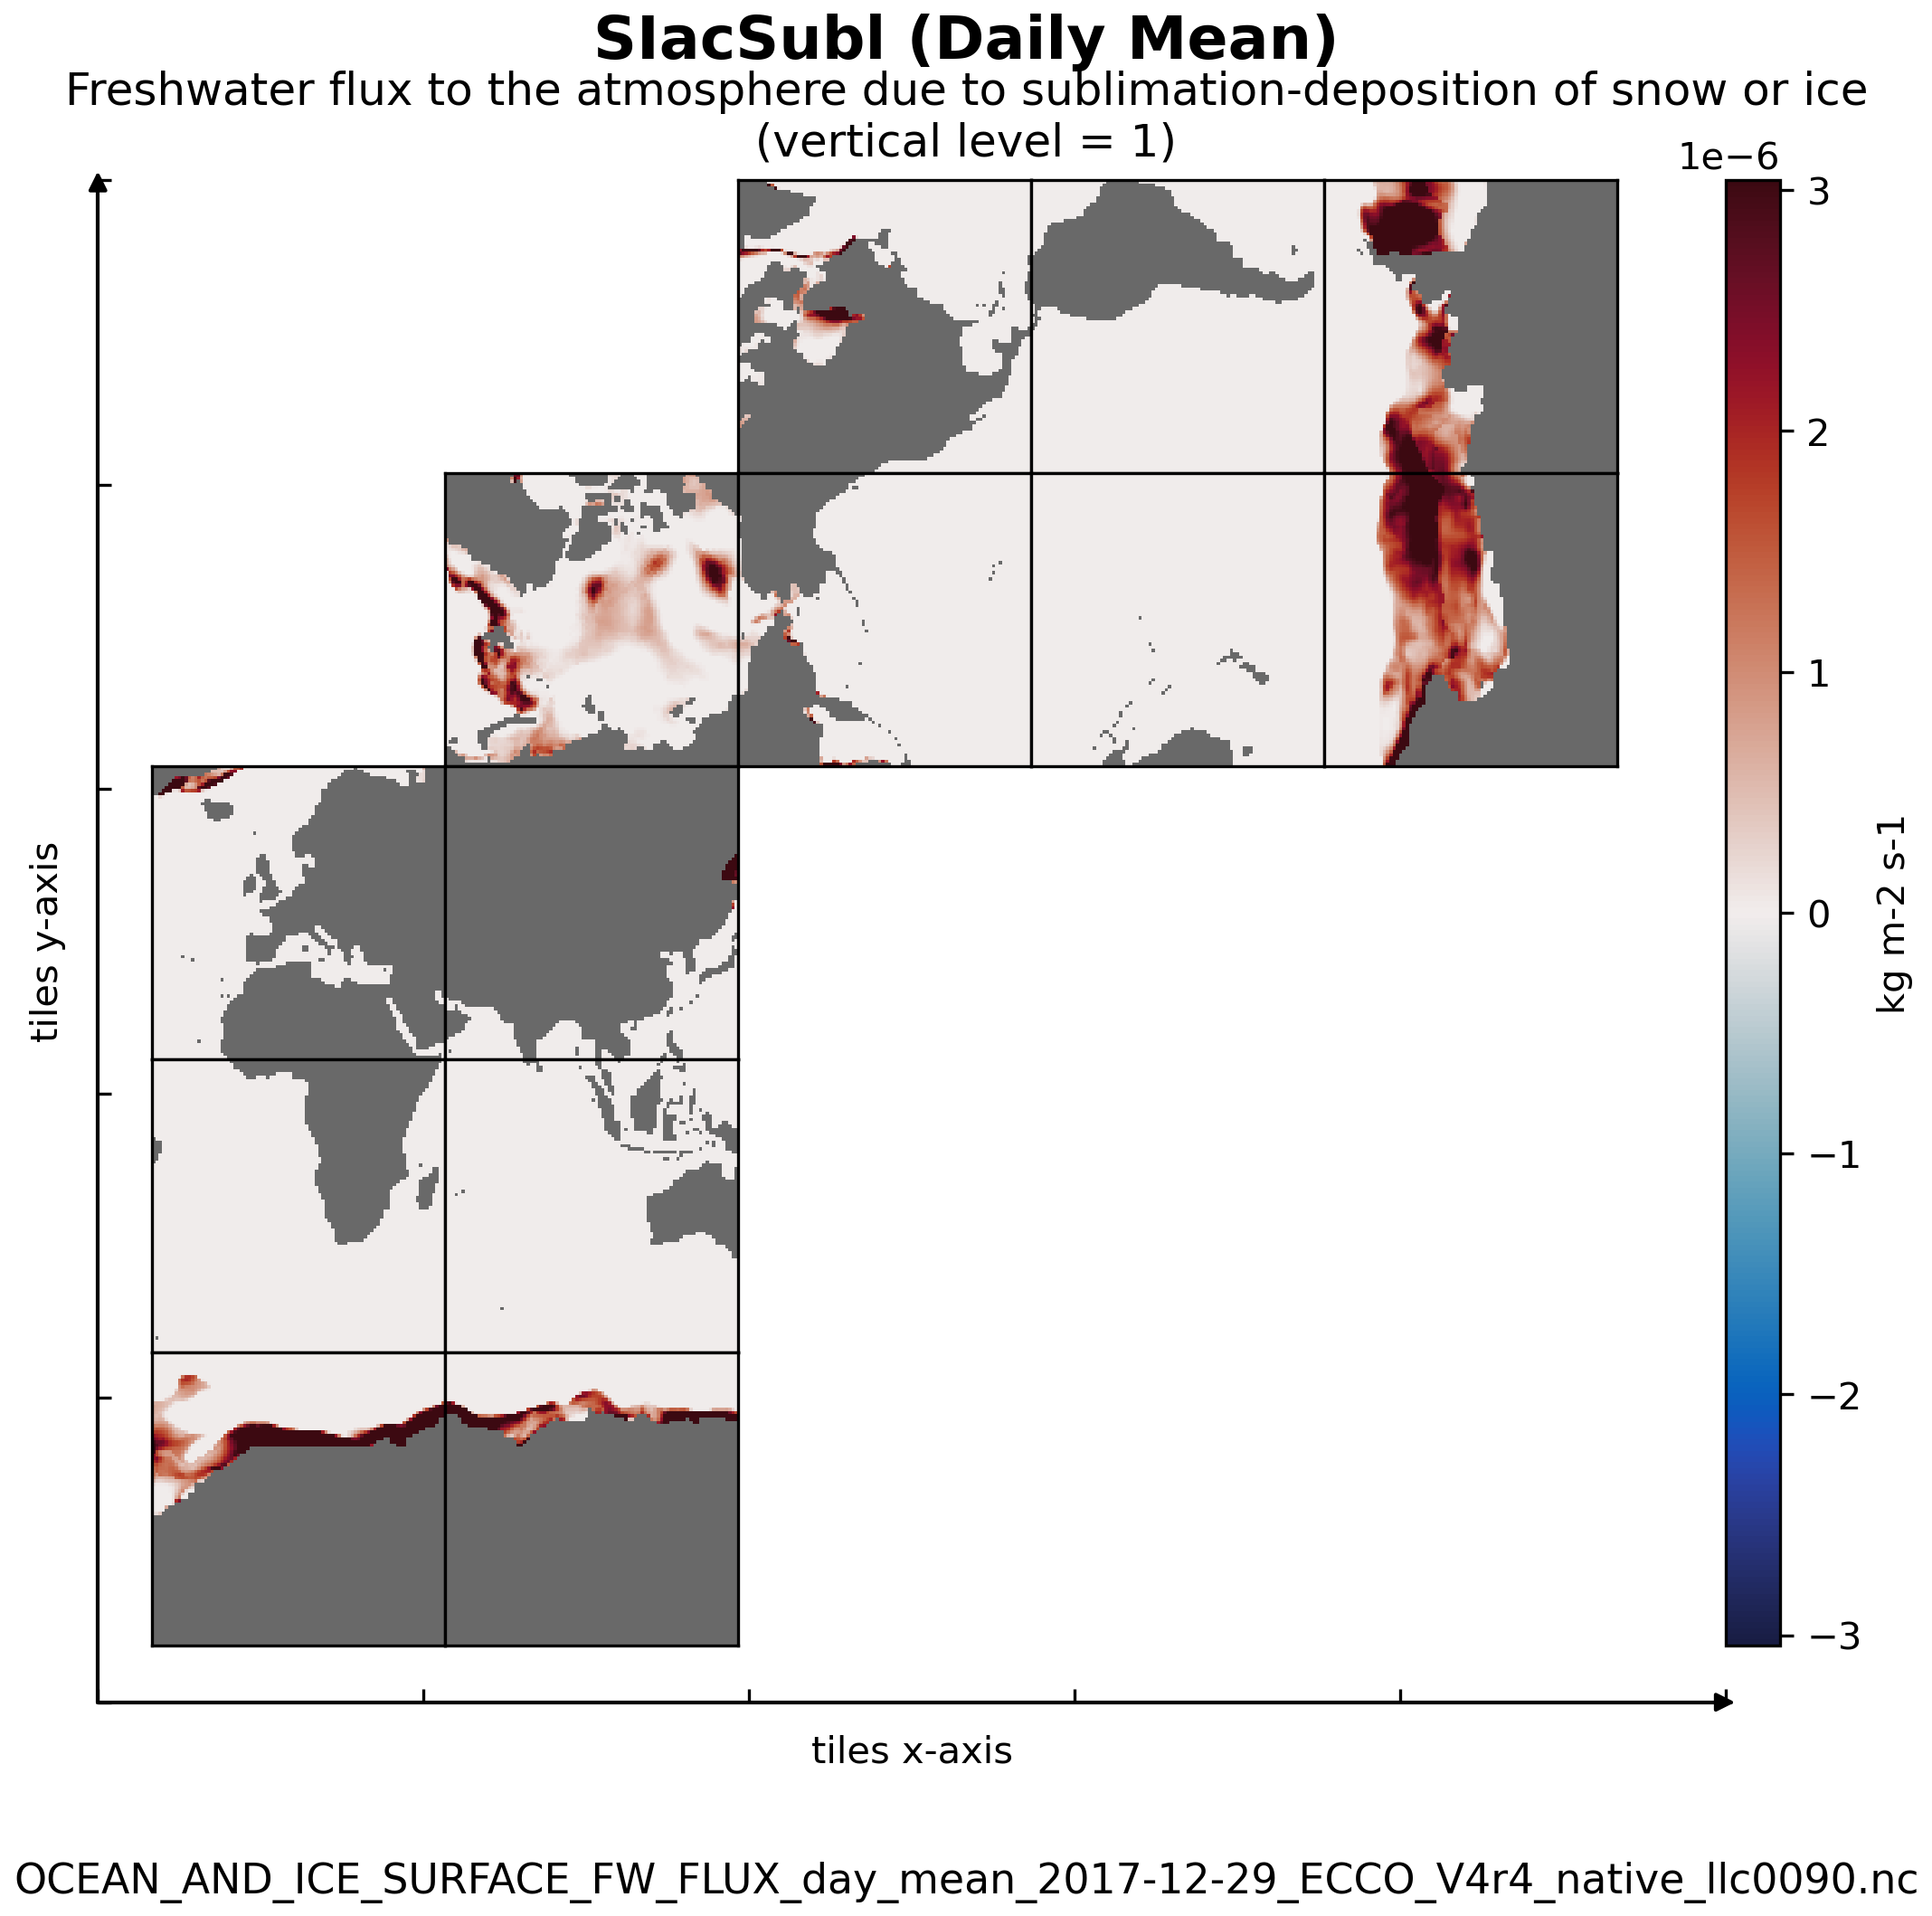
\includegraphics[scale=0.55]{../images/plots/v4r4/native_plots/Ocean_and_Sea-Ice_Surface_Freshwater_Fluxes/SIacSubl.png}
\caption{Dataset: OCEAN\_AND\_ICE\_SURFACE\_FW\_FLUX, Variable: SIacSubl}
\label{tab:table-OCEAN_AND_ICE_SURFACE_FW_FLUX_SIacSubl-Plot}
\end{figure}
\newpage
\pagebreak
\subsubsection{Native Variable: SIatmFW}
\begin{longtable}{|m{0.06\textwidth}|m{0.3\textwidth}|m{0.45\textwidth}|m{0.12\textwidth}|}
\caption{Attributes description of the variable 'SIatmFW' from OCEAN\_AND\_ICE\_SURFACE\_FW\_FLUX's  dataset.}
\label{tab:table-OCEAN_AND_ICE_SURFACE_FW_FLUX_SIatmFW} \\ 
\hline \endhead \hline \endfoot
\rowcolor{lightgray} \textbf{Storage Type} & \textbf{Variable Name} & \textbf{Description} & \textbf{Unit} \\ \hline
float32 & SIatmFW & Net freshwater flux into the open ocean, sea-ice, and snow & kg m-2 s-1 \\ \hline
\multicolumn{4}{|c|}{\cellcolor{lightgray}{\textbf{Description of the variable in Common Data language (CDL)}}} \\ \hline
\multicolumn{4}{|c|}{\fontfamily{lmtt}\selectfont{\makecell{\parbox{.95\textwidth}{\vspace*{0.25cm} \footnotesize{float32 SIatmFW(time, tile, j, i)\\
\hspace*{0.5cm}SIatmFW: \_FillValue = 9.96921e+36\\
\hspace*{0.5cm}SIatmFW: coordinates = YC XC time\\
\hspace*{0.5cm}SIatmFW: coverage\_content\_type = modelResult\\
\hspace*{0.5cm}SIatmFW: direction = >0 decreases salinity (SALT)\\
\hspace*{0.5cm}SIatmFW: long\_name = Net freshwater flux into the open ocean, sea-ice, and snow\\
\hspace*{0.5cm}SIatmFW: standard\_name = surface downward water flux\\
\hspace*{0.5cm}SIatmFW: units = kg m-2 s-1\\
\hspace*{0.5cm}SIatmFW: valid\_max = 0.008299433626234531\\
\hspace*{0.5cm}SIatmFW: valid\_min = -0.00043017856660299003\\
}}}}} \\ \hline
\rowcolor{lightgray} \multicolumn{4}{|c|}{\textbf{Comments}} \\ \hline
\multicolumn{4}{|p{1\textwidth}|}{\footnotesize{{Net freshwater flux into the combined liquid ocean, sea-ice, and snow reservoirs from the atmosphere and runoff. note: freshwater fluxes between the liquid ocean and sea-ice or snow reservoirs do not contribute to siatmfw. siatmfw counts all fluxes to/from the atmosphere that change the total freshwater stored in the combined liquid ocean, sea-ice, and snow reservoirs.}}} \\ \hline
\end{longtable}

\begin{figure}[H]
\centering
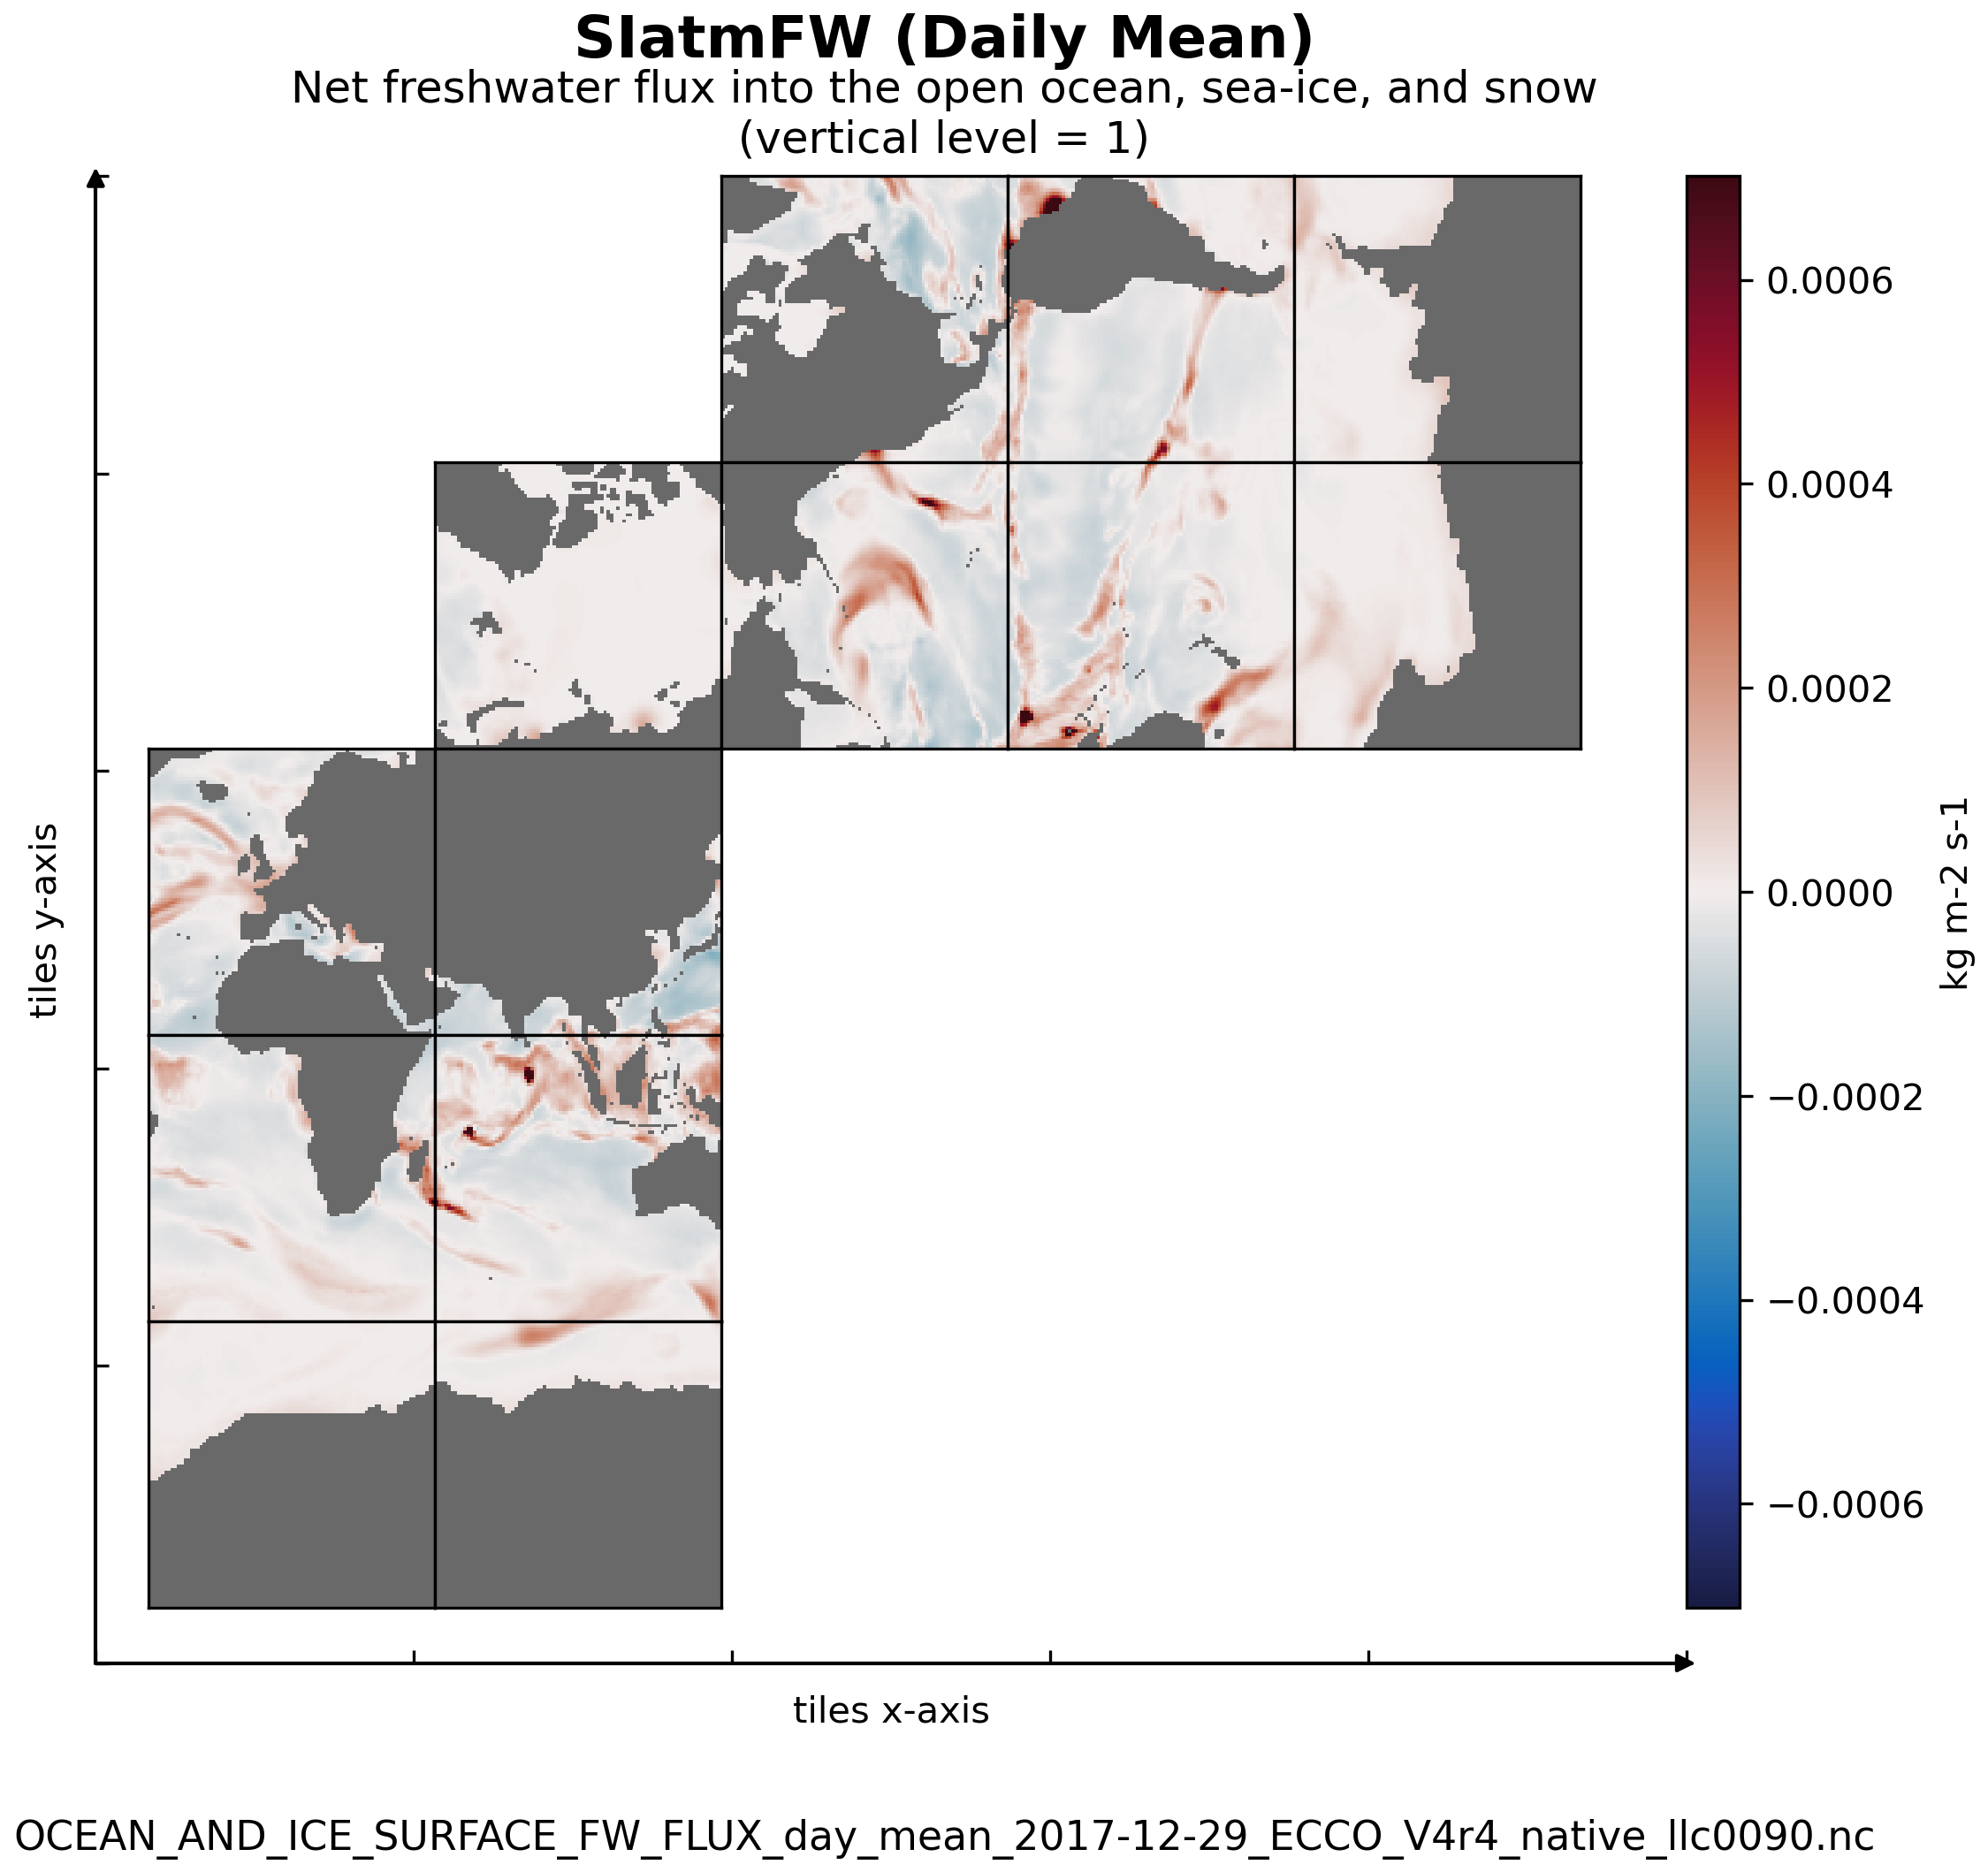
\includegraphics[scale=0.55]{../images/plots/v4r4/native_plots/Ocean_and_Sea-Ice_Surface_Freshwater_Fluxes/SIatmFW.png}
\caption{Dataset: OCEAN\_AND\_ICE\_SURFACE\_FW\_FLUX, Variable: SIatmFW}
\label{tab:table-OCEAN_AND_ICE_SURFACE_FW_FLUX_SIatmFW-Plot}
\end{figure}
\newpage
\pagebreak
\subsubsection{Native Variable: SIfwThru}
\begin{longtable}{|m{0.06\textwidth}|m{0.3\textwidth}|m{0.45\textwidth}|m{0.12\textwidth}|}
\caption{Attributes description of the variable 'SIfwThru' from OCEAN\_AND\_ICE\_SURFACE\_FW\_FLUX's  dataset.}
\label{tab:table-OCEAN_AND_ICE_SURFACE_FW_FLUX_SIfwThru} \\ 
\hline \endhead \hline \endfoot
\rowcolor{lightgray} \textbf{Storage Type} & \textbf{Variable Name} & \textbf{Description} & \textbf{Unit} \\ \hline
float32 & SIfwThru & Precipitation through sea-ice & kg m-2 s-1 \\ \hline
\multicolumn{4}{|c|}{\cellcolor{lightgray}{\textbf{Description of the variable in Common Data language (CDL)}}} \\ \hline
\multicolumn{4}{|c|}{\fontfamily{lmtt}\selectfont{\makecell{\parbox{.95\textwidth}{\vspace*{0.25cm} \footnotesize{float32 SIfwThru(time, tile, j, i)\\
\hspace*{0.5cm}SIfwThru: \_FillValue = 9.96921e+36\\
\hspace*{0.5cm}SIfwThru: coordinates = YC XC time\\
\hspace*{0.5cm}SIfwThru: coverage\_content\_type = modelResult\\
\hspace*{0.5cm}SIfwThru: direction = >0 increases ocean volume\\
\hspace*{0.5cm}SIfwThru: long\_name = Precipitation through sea-ice\\
\hspace*{0.5cm}SIfwThru: units = kg m-2 s-1\\
\hspace*{0.5cm}SIfwThru: valid\_max = 0.0010632629273459315\\
\hspace*{0.5cm}SIfwThru: valid\_min = -1.695218452368863e-05\\
}}}}} \\ \hline
\rowcolor{lightgray} \multicolumn{4}{|c|}{\textbf{Comments}} \\ \hline
\multicolumn{4}{|p{1\textwidth}|}{\footnotesize{{Precipitation over sea-ice covered regions reaching ocean through sea-ice. note: precipitation over sea-ice covered regions that directly reaches ocean through the sea-ice. it is not due to melt of sea-ice/snow.}}} \\ \hline
\end{longtable}

\begin{figure}[H]
\centering
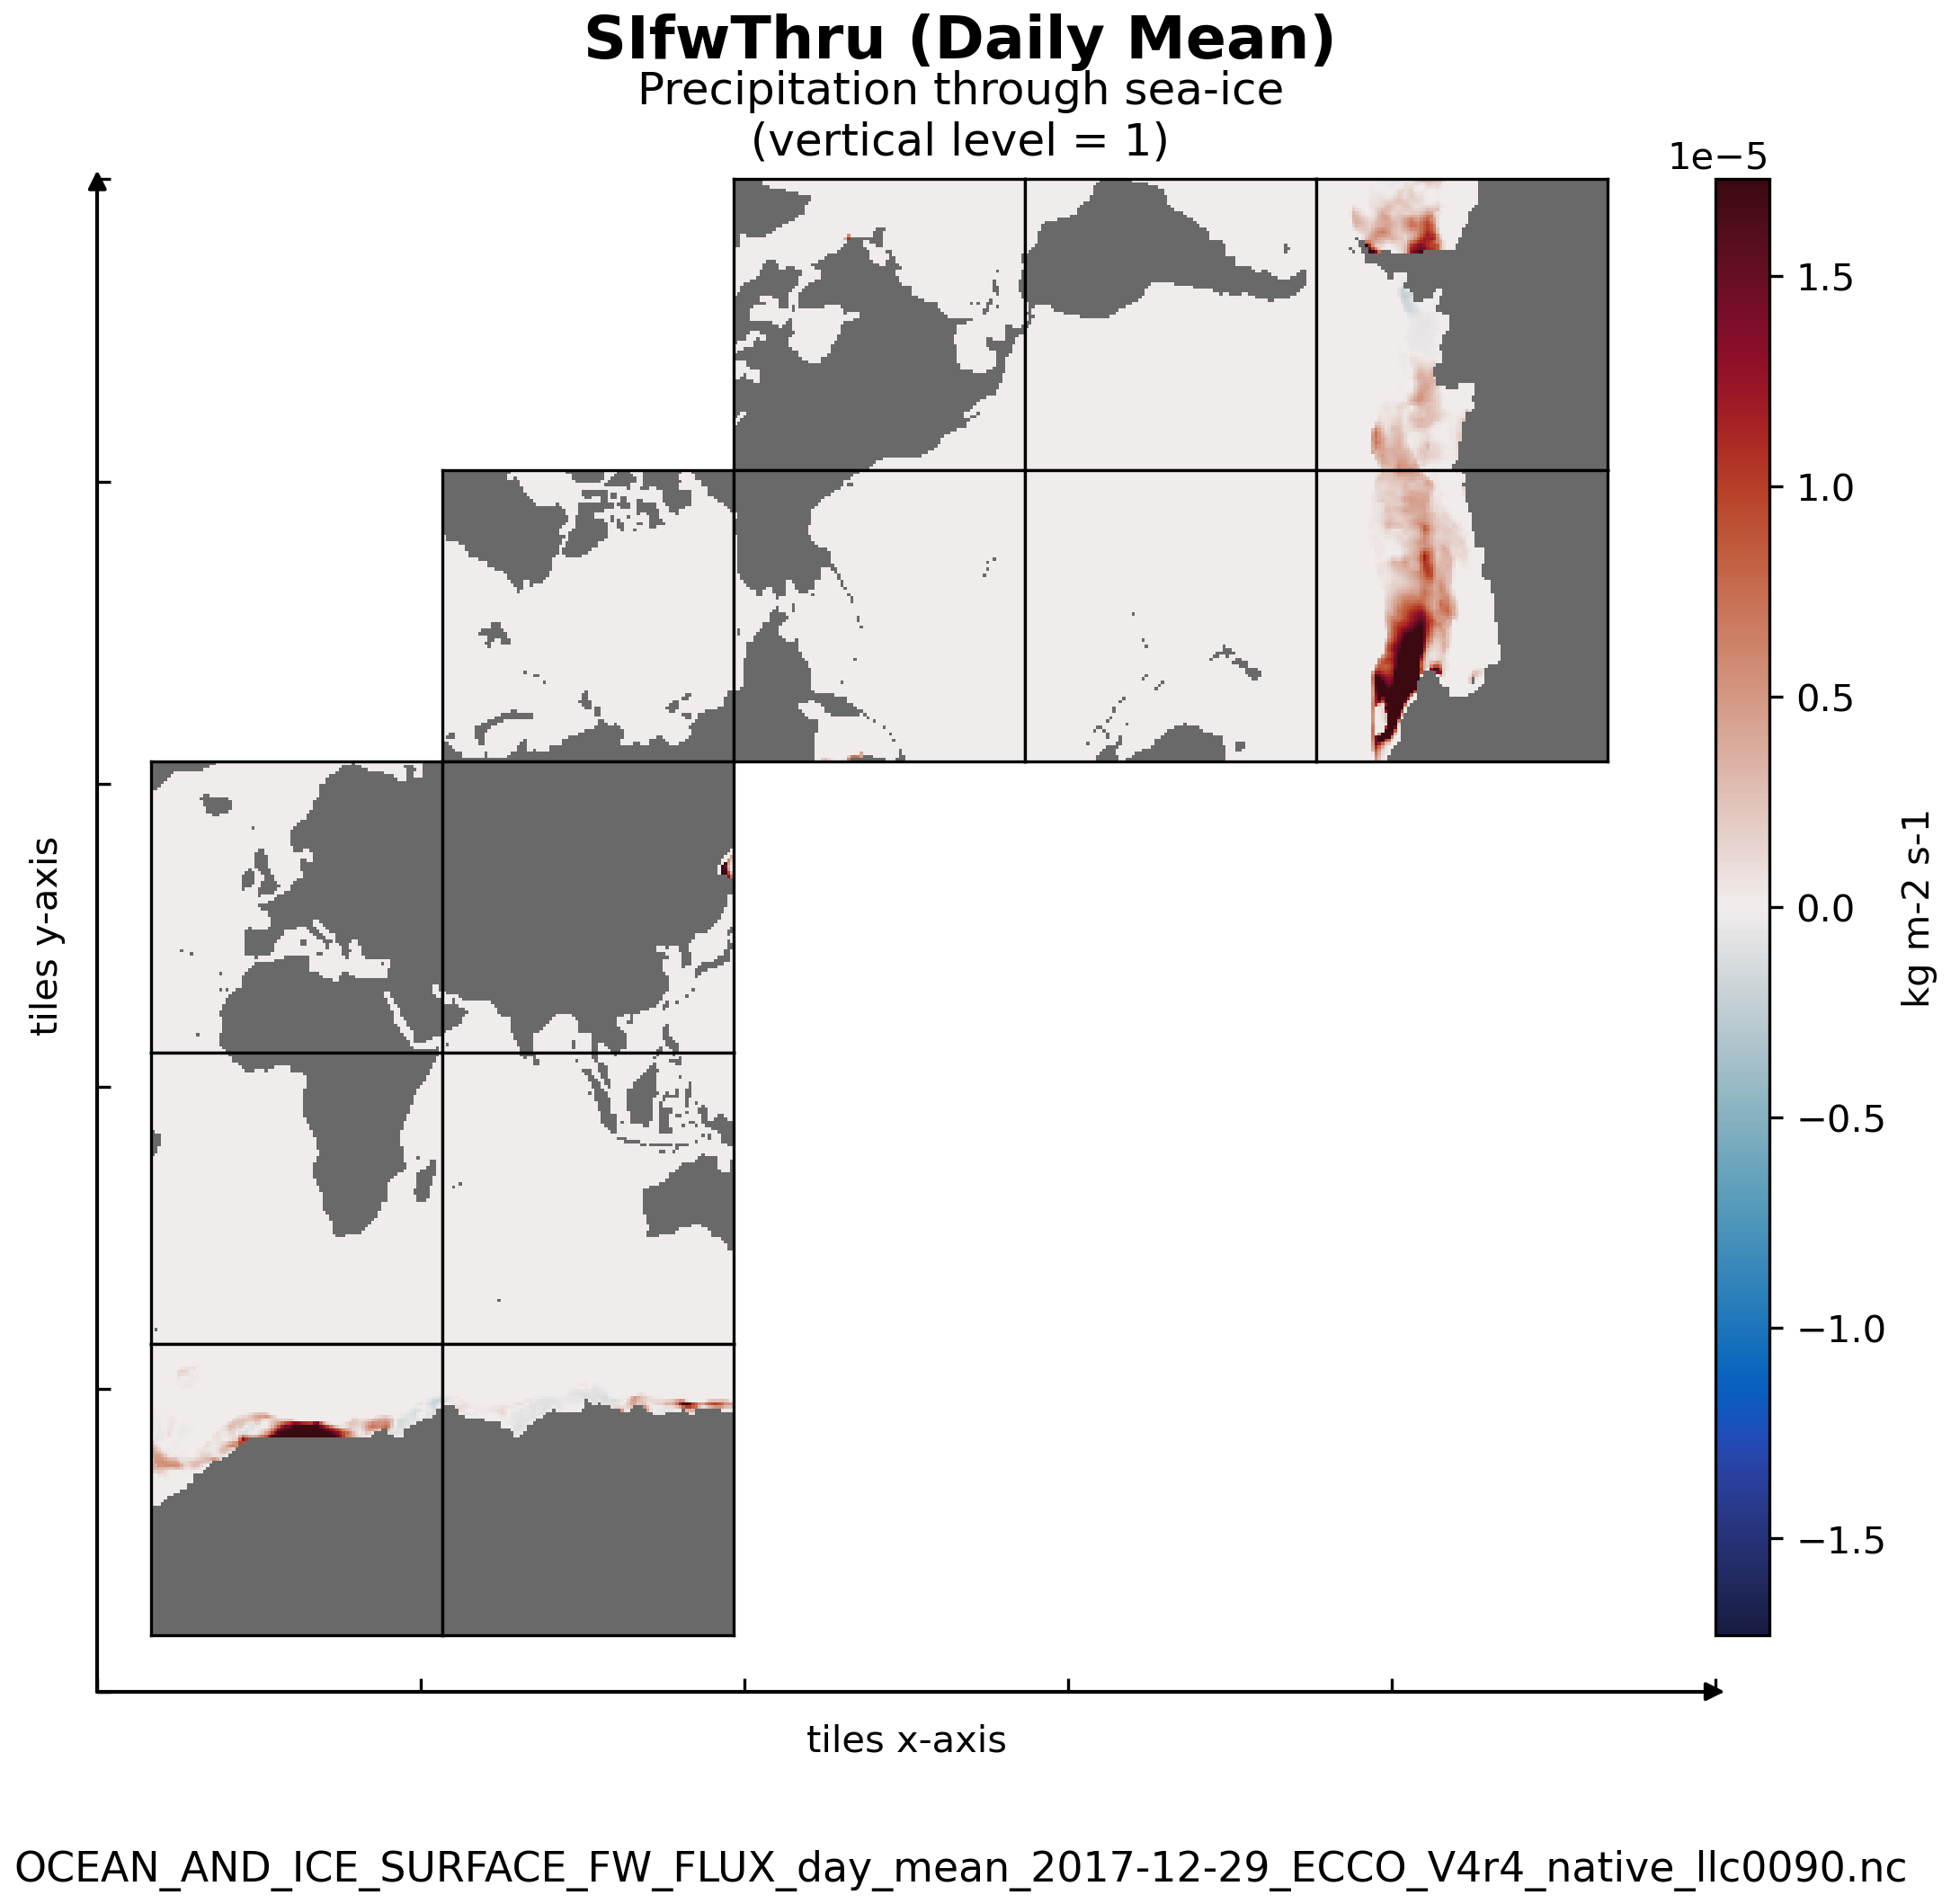
\includegraphics[scale=0.55]{../images/plots/v4r4/native_plots/Ocean_and_Sea-Ice_Surface_Freshwater_Fluxes/SIfwThru.png}
\caption{Dataset: OCEAN\_AND\_ICE\_SURFACE\_FW\_FLUX, Variable: SIfwThru}
\label{tab:table-OCEAN_AND_ICE_SURFACE_FW_FLUX_SIfwThru-Plot}
\end{figure}
\newpage
\pagebreak
\subsubsection{Native Variable: SIrsSubl}
\begin{longtable}{|m{0.06\textwidth}|m{0.3\textwidth}|m{0.45\textwidth}|m{0.12\textwidth}|}
\caption{Attributes description of the variable 'SIrsSubl' from OCEAN\_AND\_ICE\_SURFACE\_FW\_FLUX's  dataset.}
\label{tab:table-OCEAN_AND_ICE_SURFACE_FW_FLUX_SIrsSubl} \\ 
\hline \endhead \hline \endfoot
\rowcolor{lightgray} \textbf{Storage Type} & \textbf{Variable Name} & \textbf{Description} & \textbf{Unit} \\ \hline
float32 & SIrsSubl & Residual sublimation freshwater flux & kg m-2 s-1 \\ \hline
\multicolumn{4}{|c|}{\cellcolor{lightgray}{\textbf{Description of the variable in Common Data language (CDL)}}} \\ \hline
\multicolumn{4}{|c|}{\fontfamily{lmtt}\selectfont{\makecell{\parbox{.95\textwidth}{\vspace*{0.25cm} \footnotesize{float32 SIrsSubl(time, tile, j, i)\\
\hspace*{0.5cm}SIrsSubl: \_FillValue = 9.96921e+36\\
\hspace*{0.5cm}SIrsSubl: coordinates = YC XC time\\
\hspace*{0.5cm}SIrsSubl: coverage\_content\_type = modelResult\\
\hspace*{0.5cm}SIrsSubl: direction = >0 decreases ocean volume\\
\hspace*{0.5cm}SIrsSubl: long\_name = Residual sublimation freshwater flux\\
\hspace*{0.5cm}SIrsSubl: units = kg m-2 s-1\\
\hspace*{0.5cm}SIrsSubl: valid\_max = 8.640533451398369e-06\\
\hspace*{0.5cm}SIrsSubl: valid\_min = -0.0001067528864950873\\
}}}}} \\ \hline
\rowcolor{lightgray} \multicolumn{4}{|c|}{\textbf{Comments}} \\ \hline
\multicolumn{4}{|p{1\textwidth}|}{\footnotesize{{Residual freshwater flux by sublimation to remove water from or add water to ocean. when implied sublimation freshwater flux siacsubl is larger than availabe sea-ice/snow, sirssubl is positive and water is removed from ocean. note: freshwater flux by sublimation that is to remove water from the ocean when it is positive.}}} \\ \hline
\end{longtable}

\begin{figure}[H]
\centering
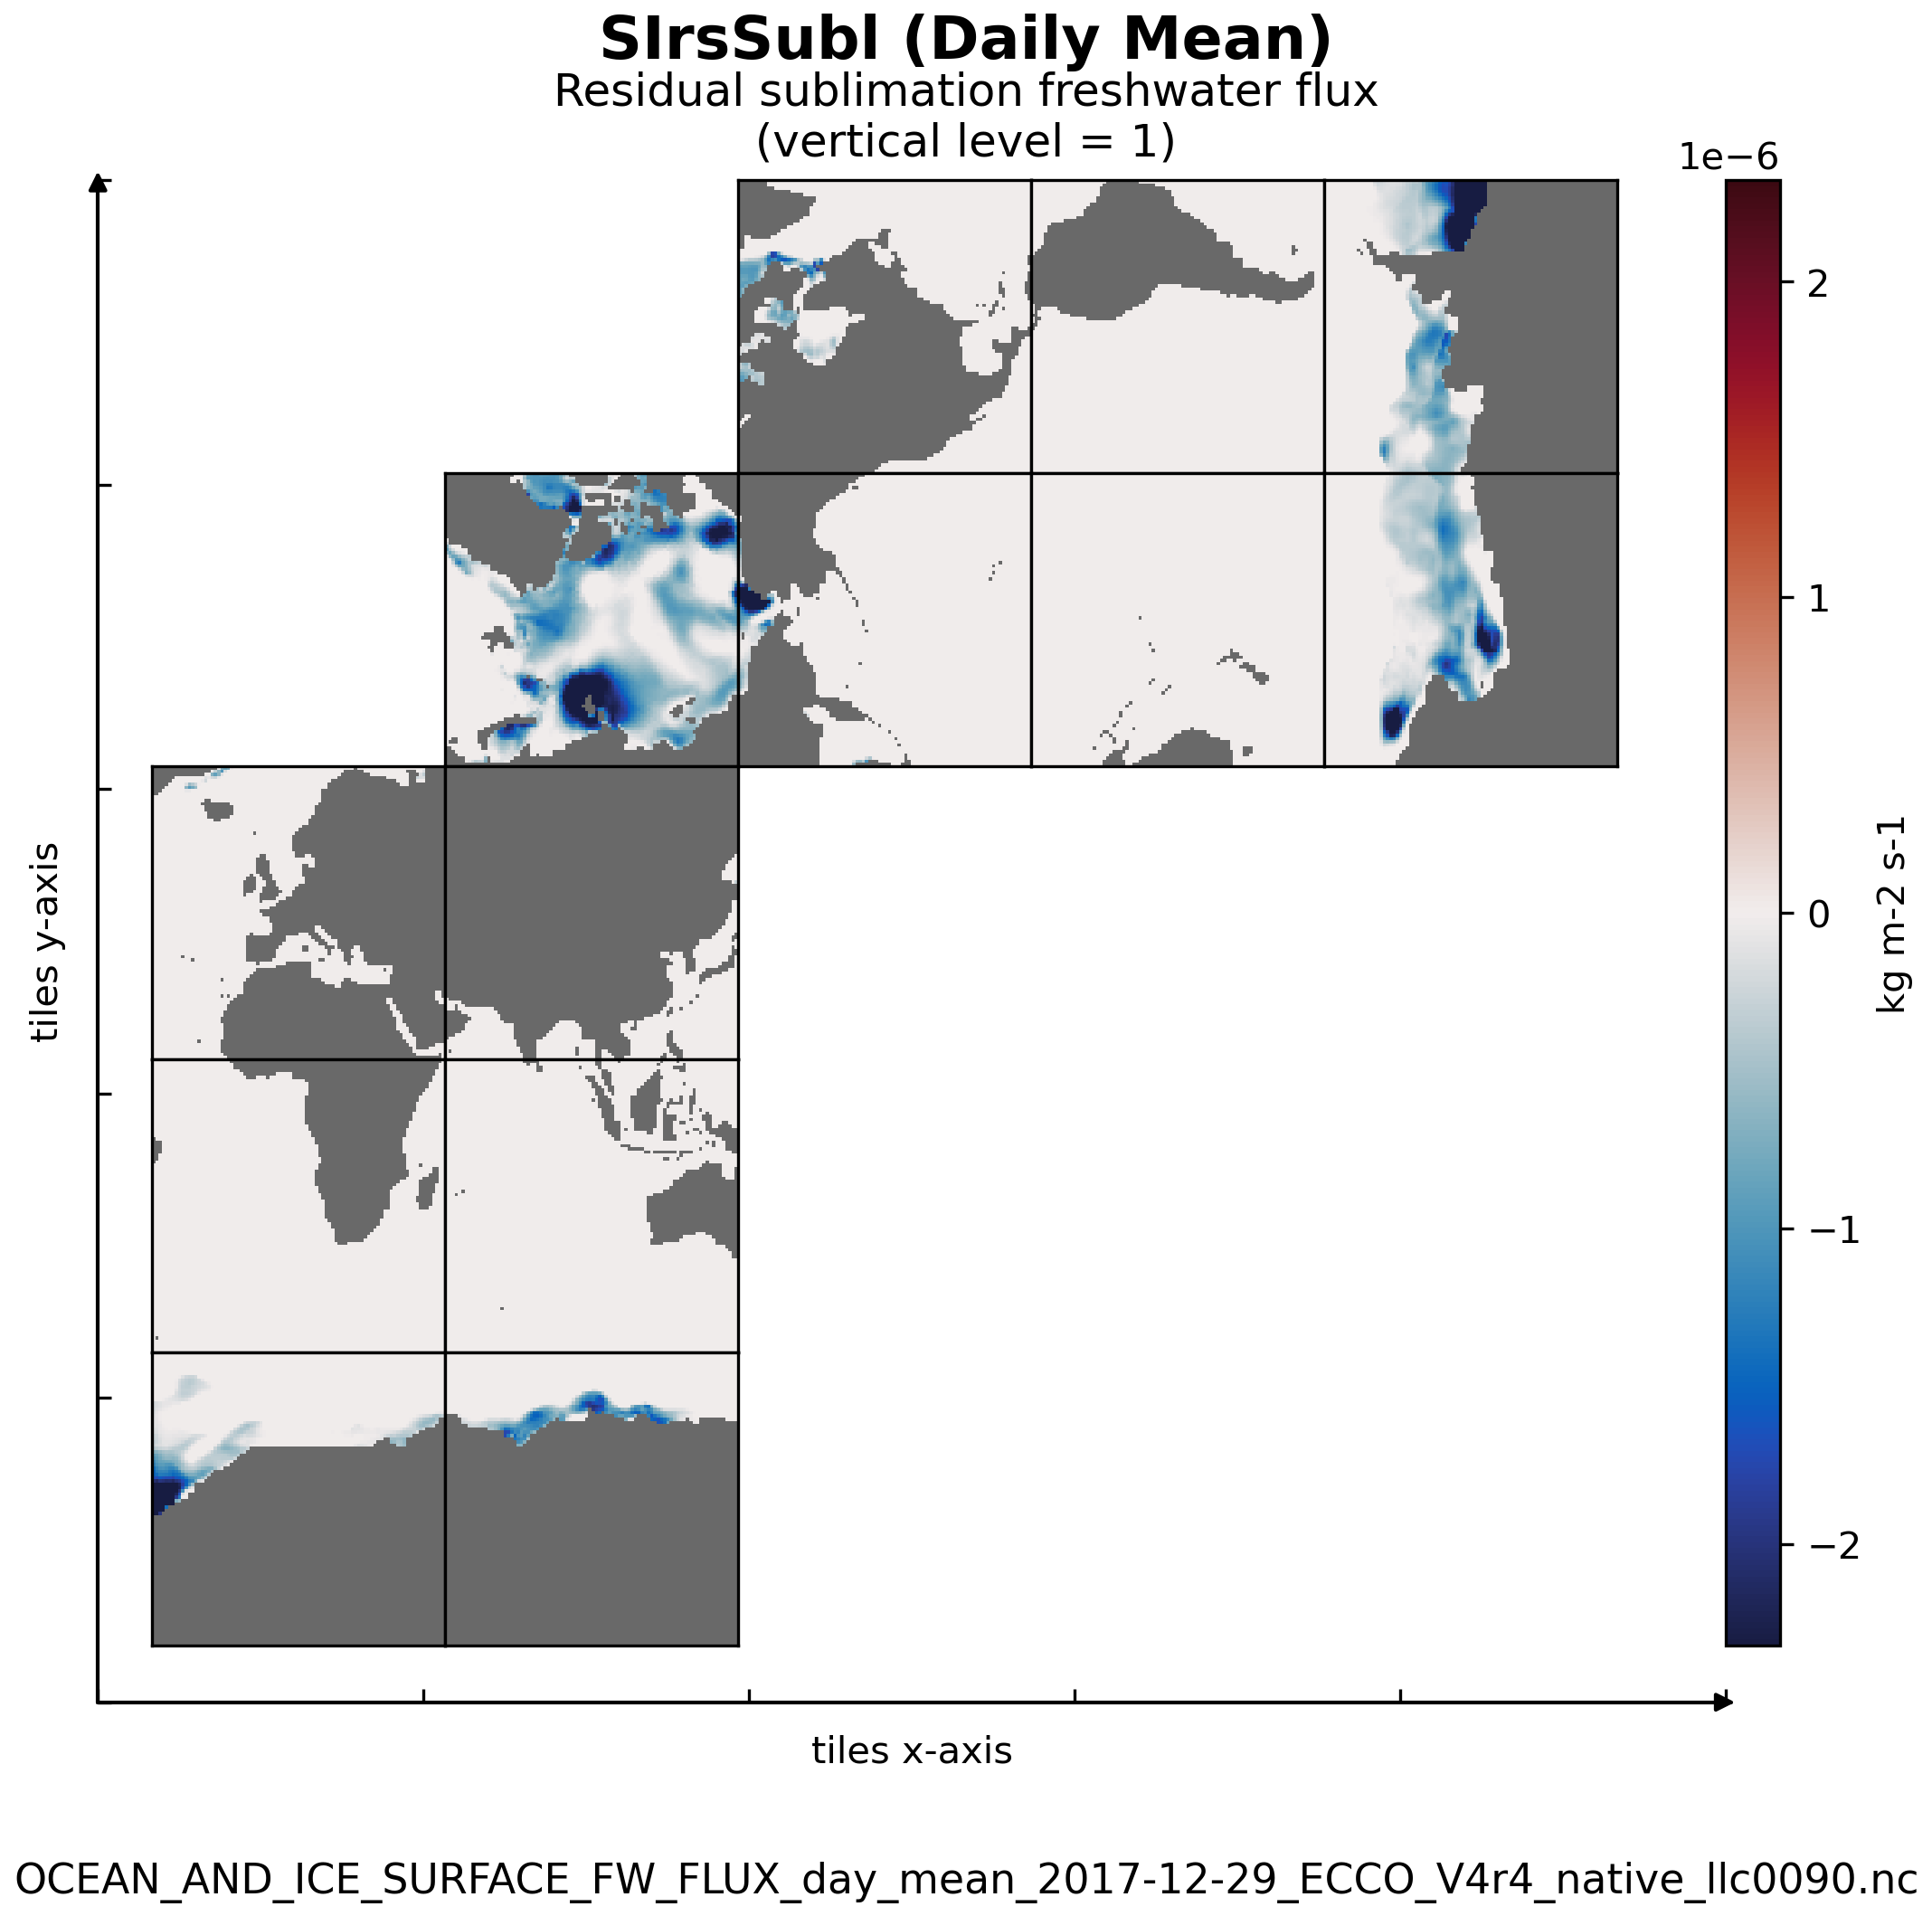
\includegraphics[scale=0.55]{../images/plots/v4r4/native_plots/Ocean_and_Sea-Ice_Surface_Freshwater_Fluxes/SIrsSubl.png}
\caption{Dataset: OCEAN\_AND\_ICE\_SURFACE\_FW\_FLUX, Variable: SIrsSubl}
\label{tab:table-OCEAN_AND_ICE_SURFACE_FW_FLUX_SIrsSubl-Plot}
\end{figure}
\newpage
\pagebreak
\subsubsection{Native Variable: SIsnPrcp}
\begin{longtable}{|m{0.06\textwidth}|m{0.3\textwidth}|m{0.45\textwidth}|m{0.12\textwidth}|}
\caption{Attributes description of the variable 'SIsnPrcp' from OCEAN\_AND\_ICE\_SURFACE\_FW\_FLUX's  dataset.}
\label{tab:table-OCEAN_AND_ICE_SURFACE_FW_FLUX_SIsnPrcp} \\ 
\hline \endhead \hline \endfoot
\rowcolor{lightgray} \textbf{Storage Type} & \textbf{Variable Name} & \textbf{Description} & \textbf{Unit} \\ \hline
float32 & SIsnPrcp & Snow precipitation on sea-ice & kg m-2 s-1 \\ \hline
\multicolumn{4}{|c|}{\cellcolor{lightgray}{\textbf{Description of the variable in Common Data language (CDL)}}} \\ \hline
\multicolumn{4}{|c|}{\fontfamily{lmtt}\selectfont{\makecell{\parbox{.95\textwidth}{\vspace*{0.25cm} \footnotesize{float32 SIsnPrcp(time, tile, j, i)\\
\hspace*{0.5cm}SIsnPrcp: \_FillValue = 9.96921e+36\\
\hspace*{0.5cm}SIsnPrcp: coordinates = YC XC time\\
\hspace*{0.5cm}SIsnPrcp: coverage\_content\_type = modelResult\\
\hspace*{0.5cm}SIsnPrcp: direction = >0 increases snow thickness (HSNOW)\\
\hspace*{0.5cm}SIsnPrcp: long\_name = Snow precipitation on sea-ice\\
\hspace*{0.5cm}SIsnPrcp: standard\_name = snowfall flux\\
\hspace*{0.5cm}SIsnPrcp: units = kg m-2 s-1\\
\hspace*{0.5cm}SIsnPrcp: valid\_max = 0.0009354020585305989\\
\hspace*{0.5cm}SIsnPrcp: valid\_min = -4.334669574745931e-05\\
}}}}} \\ \hline
\rowcolor{lightgray} \multicolumn{4}{|c|}{\textbf{Comments}} \\ \hline
\multicolumn{4}{|p{1\textwidth}|}{\footnotesize{{Snow precipitation rate over sea-ice, averaged over the entire model grid cell.}}} \\ \hline
\end{longtable}

\begin{figure}[H]
\centering
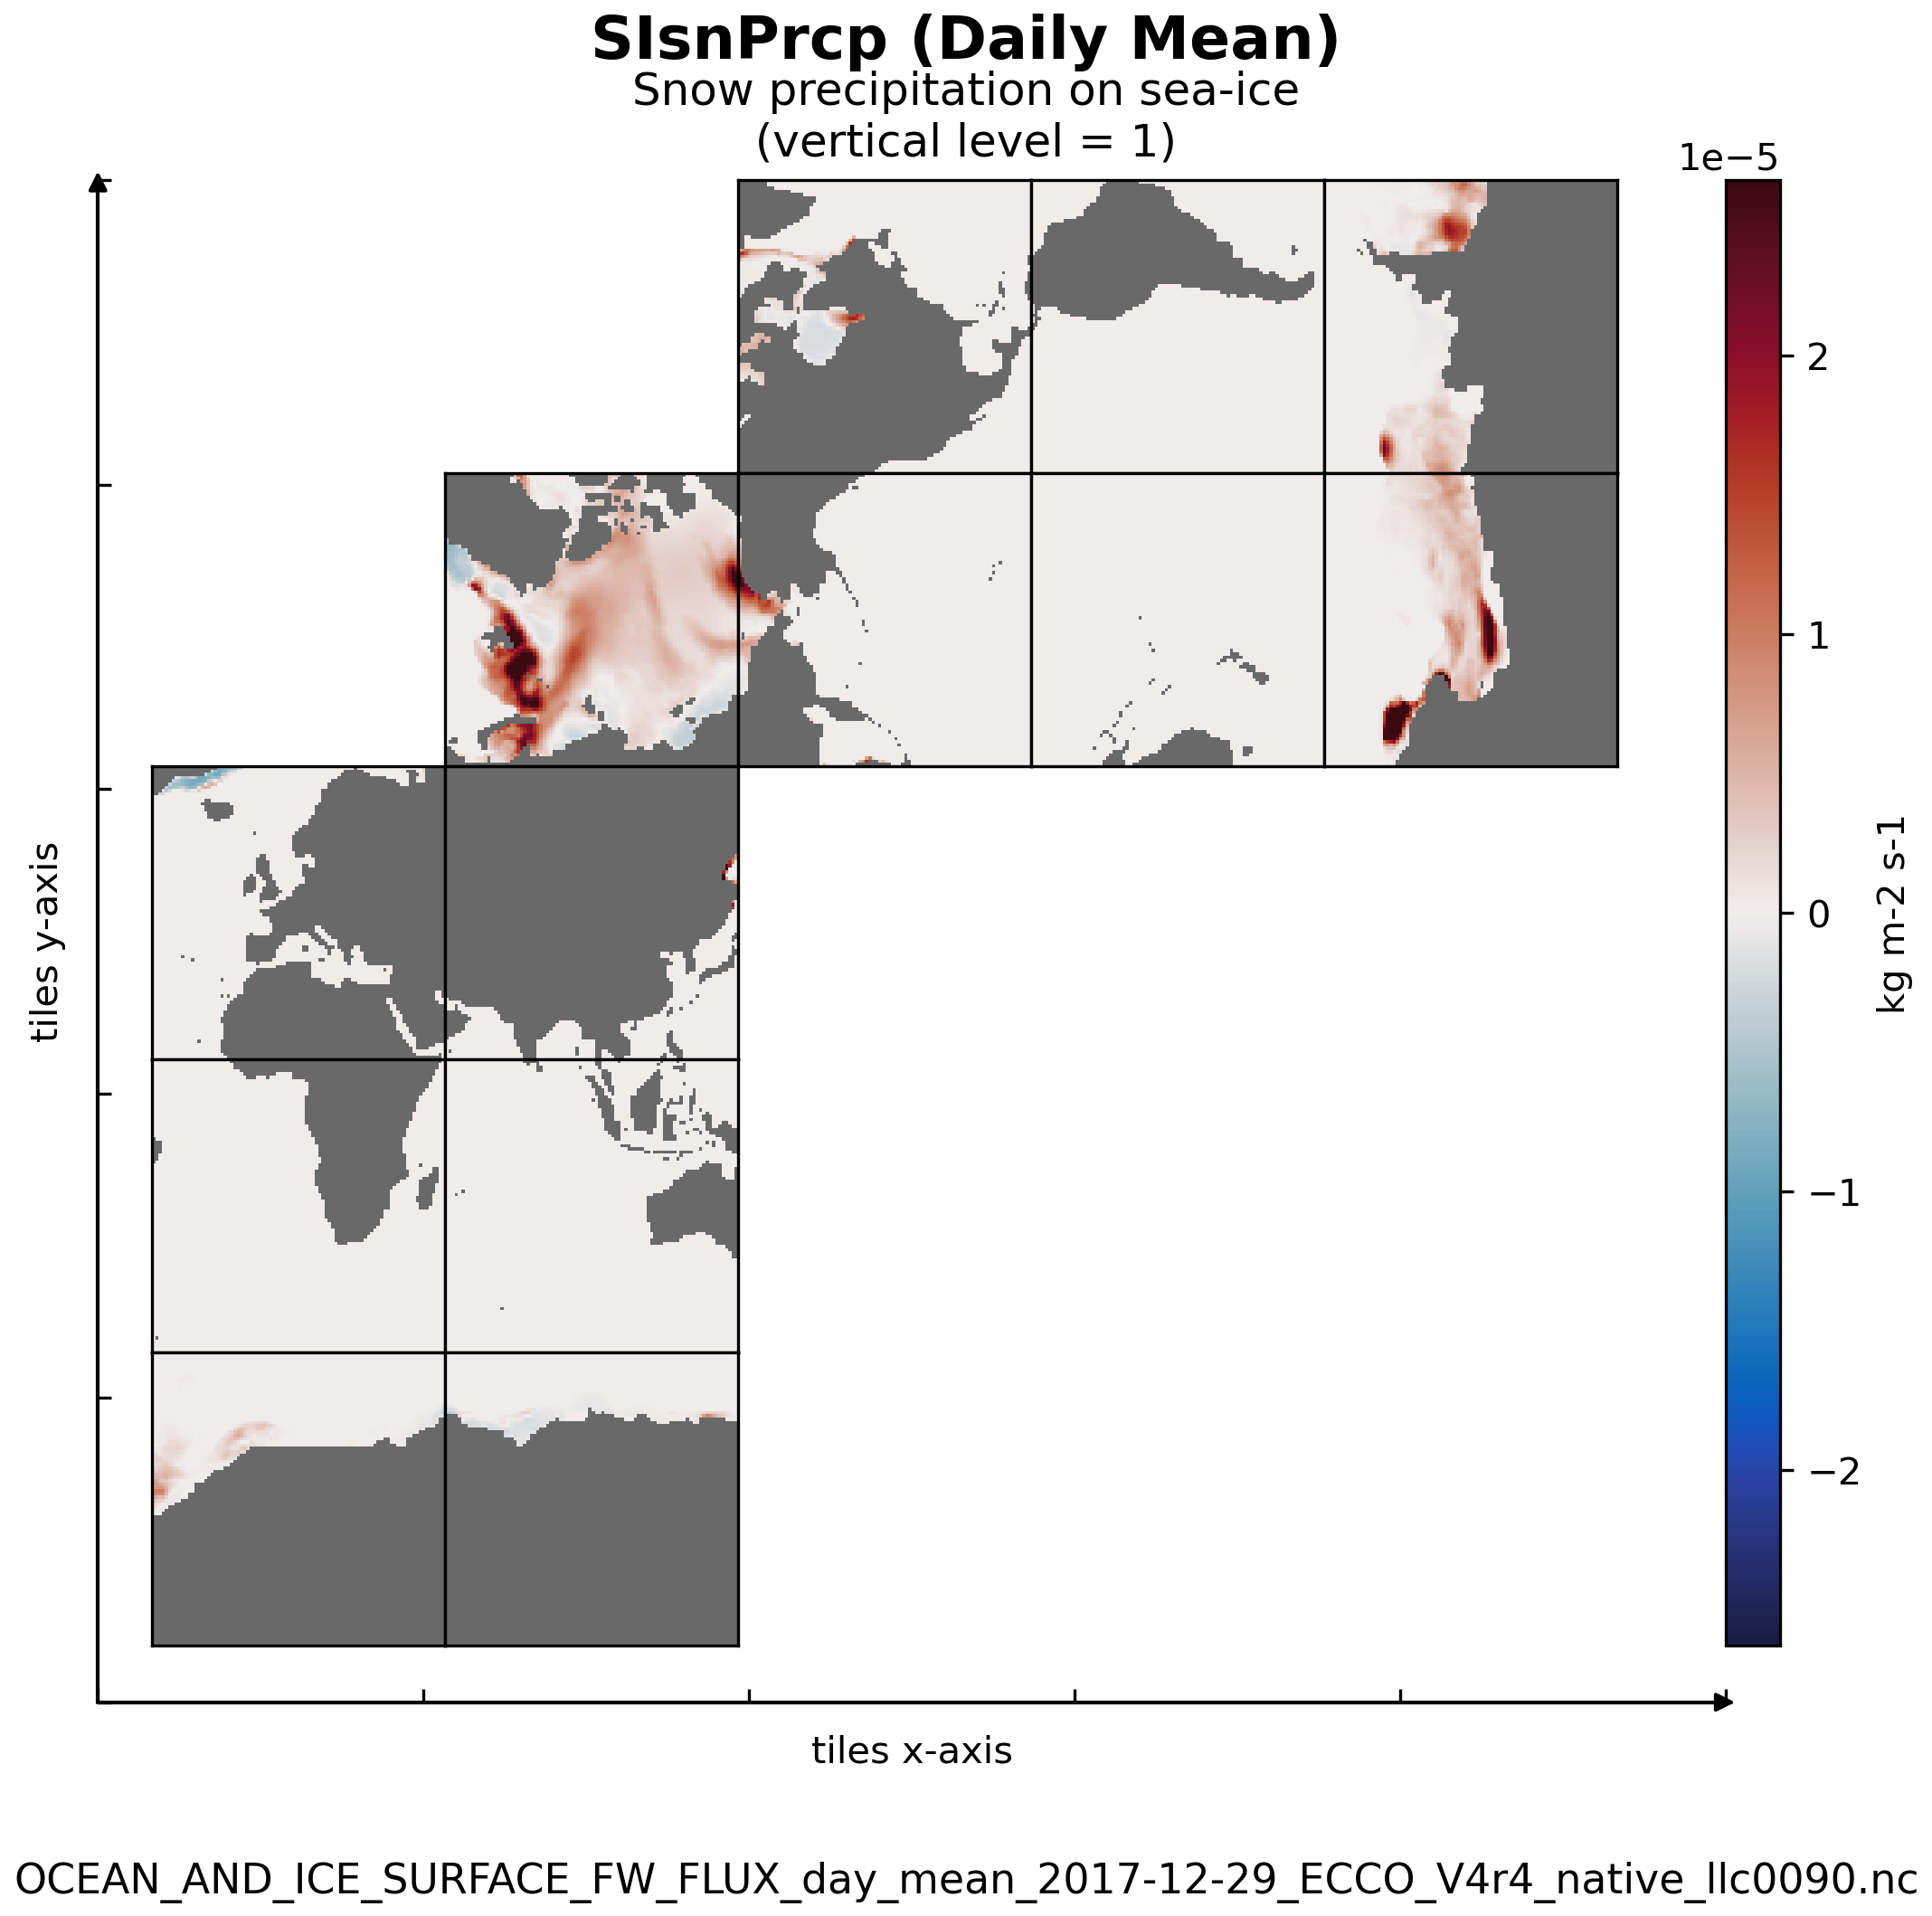
\includegraphics[scale=0.55]{../images/plots/v4r4/native_plots/Ocean_and_Sea-Ice_Surface_Freshwater_Fluxes/SIsnPrcp.png}
\caption{Dataset: OCEAN\_AND\_ICE\_SURFACE\_FW\_FLUX, Variable: SIsnPrcp}
\label{tab:table-OCEAN_AND_ICE_SURFACE_FW_FLUX_SIsnPrcp-Plot}
\end{figure}
\newpage
\pagebreak
\subsubsection{Native Variable: oceFWflx}
\begin{longtable}{|m{0.06\textwidth}|m{0.3\textwidth}|m{0.45\textwidth}|m{0.12\textwidth}|}
\caption{Attributes description of the variable 'oceFWflx' from OCEAN\_AND\_ICE\_SURFACE\_FW\_FLUX's  dataset.}
\label{tab:table-OCEAN_AND_ICE_SURFACE_FW_FLUX_oceFWflx} \\ 
\hline \endhead \hline \endfoot
\rowcolor{lightgray} \textbf{Storage Type} & \textbf{Variable Name} & \textbf{Description} & \textbf{Unit} \\ \hline
float32 & oceFWflx & Net freshwater flux into the ocean & kg m-2 s-1 \\ \hline
\multicolumn{4}{|c|}{\cellcolor{lightgray}{\textbf{Description of the variable in Common Data language (CDL)}}} \\ \hline
\multicolumn{4}{|c|}{\fontfamily{lmtt}\selectfont{\makecell{\parbox{.95\textwidth}{\vspace*{0.25cm} \footnotesize{float32 oceFWflx(time, tile, j, i)\\
\hspace*{0.5cm}oceFWflx: \_FillValue = 9.96921e+36\\
\hspace*{0.5cm}oceFWflx: coordinates = YC XC time\\
\hspace*{0.5cm}oceFWflx: coverage\_content\_type = modelResult\\
\hspace*{0.5cm}oceFWflx: direction = >0 decreases salinity (SALT)\\
\hspace*{0.5cm}oceFWflx: long\_name = Net freshwater flux into the ocean\\
\hspace*{0.5cm}oceFWflx: standard\_name = water flux into sea water\\
\hspace*{0.5cm}oceFWflx: units = kg m-2 s-1\\
\hspace*{0.5cm}oceFWflx: valid\_max = 0.008299433626234531\\
\hspace*{0.5cm}oceFWflx: valid\_min = -0.003914969973266125\\
}}}}} \\ \hline
\rowcolor{lightgray} \multicolumn{4}{|c|}{\textbf{Comments}} \\ \hline
\multicolumn{4}{|p{1\textwidth}|}{\footnotesize{{Net freshwater flux into the ocean including contributions from runoff, evaporation, precipitation, and mass exchange with sea-ice due to melting and freezing and snow melting. note: ocefwflx does not include freshwater fluxes between the atmosphere and sea-ice and snow. the variable 'siatmfw' accounts for freshwater fluxes out of the combined ocean+sea-ice+snow reservoir.}}} \\ \hline
\end{longtable}

\begin{figure}[H]
\centering
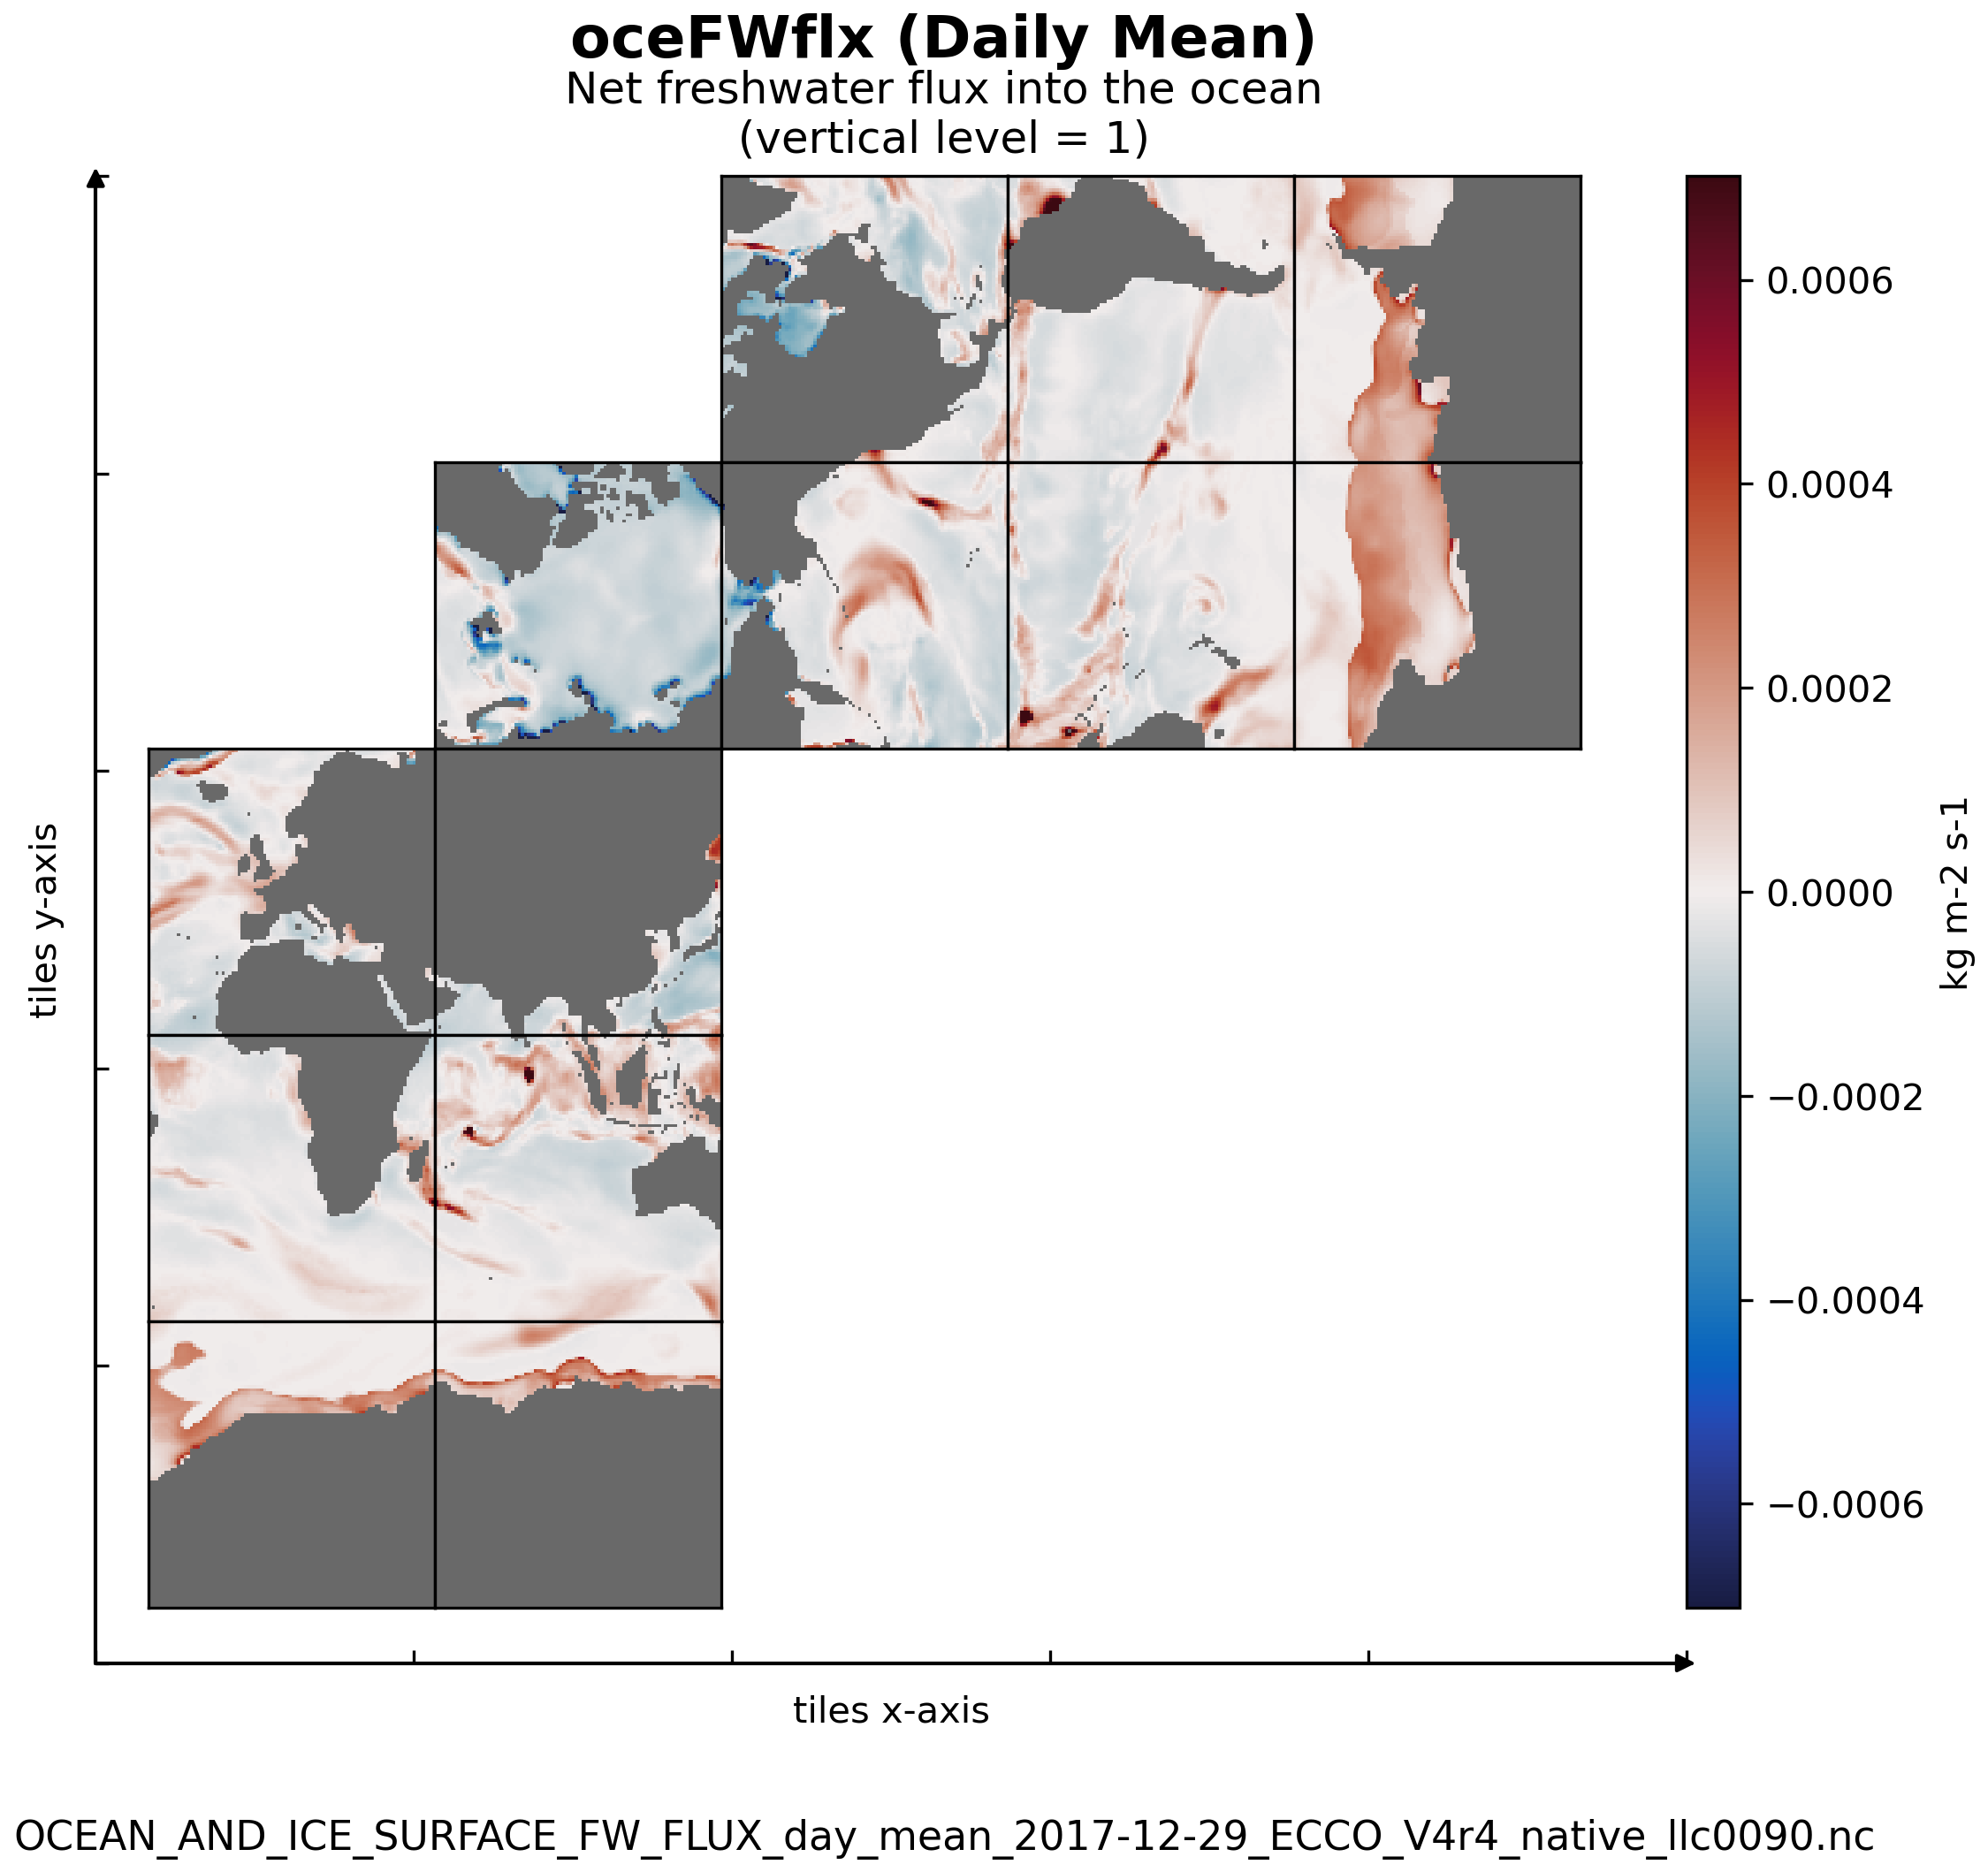
\includegraphics[scale=0.55]{../images/plots/v4r4/native_plots/Ocean_and_Sea-Ice_Surface_Freshwater_Fluxes/oceFWflx.png}
\caption{Dataset: OCEAN\_AND\_ICE\_SURFACE\_FW\_FLUX, Variable: oceFWflx}
\label{tab:table-OCEAN_AND_ICE_SURFACE_FW_FLUX_oceFWflx-Plot}
\end{figure}
\newpage
\subsection{Native dataset of OCEAN\_AND\_ICE\_SURFACE\_HEAT\_FLUX}
\newp
\subsubsection{Overview}
This dataset provides 2D fields of ocean and sea-ice surface heat fluxes on the lat-lon-cap 90 (llc90) native model grid from the ECCO Version 4 Release 4 (V4r4) ocean and sea-ice state estimate. The dataset is provided on daily-average and monthly-average time resolution. 
\begin{longtable}{|m{0.15\textwidth}|m{0.64\textwidth}|m{0.12\textwidth}|}
\caption{Coordinates and Variables in the dataset OCEAN\_AND\_ICE\_SURFACE\_HEAT\_FLUX}
\label{tab:table-OCEAN_AND_ICE_SURFACE_HEAT_FLUX-fields} \\ 
\hline \endhead \hline \endfoot
\rowcolor{lightgray} \multicolumn{1}{|c|}{\textbf{Coordinates}} & \multicolumn{1}{|c|}{\textbf{Description of data coordinates}} &  \multicolumn{1}{|c|}{\textbf{Unit}}\\ \hline
i &Grid index in x for variables at tracer and 'v' locations &--none--  \\ \hline
i\_g &Grid index in x for variables at 'u' and 'g' locations &--none--  \\ \hline
j &Grid index in y for variables at tracer and 'u' locations &--none--  \\ \hline
j\_g &Grid index in y for variables at 'v' and 'g' locations &--none--  \\ \hline
tile &Lat-lon-cap tile index &--none--  \\ \hline
time &Center time of averaging period &--none--  \\ \hline
XC &Longitude of tracer grid cell center &degrees\_east  \\ \hline
YC &Latitude of tracer grid cell center &degrees\_north  \\ \hline
XG &Longitude of 'southwest' corner of tracer grid cell &degrees\_east  \\ \hline
YG &Latitude of 'southwest' corner of tracer grid cell &degrees\_north  \\ \hline
time\_bnds &Time bounds of averaging period &--none--  \\ \hline
XC\_bnds &Longitudes of tracer grid cell corners &--none--  \\ \hline
YC\_bnds &Latitudes of tracer grid cell corners &--none--  \\ \hline
\rowcolor{lightgray} \multicolumn{1}{|c|}{\textbf{Variables}} & \multicolumn{1}{|c|}{\textbf{Description of data variables}} &  \multicolumn{1}{|c|}{\textbf{Unit}}\\ \hline
EXFhl &Open ocean air-sea latent heat flux &W m-2  \\ \hline
EXFhs &Open ocean air-sea sensible heat flux &W m-2  \\ \hline
EXFlwdn &Downward longwave radiative flux &W m-2  \\ \hline
EXFswdn &Downwelling shortwave radiative flux &W m-2  \\ \hline
EXFqnet &Open ocean net air-sea heat flux &W m-2  \\ \hline
oceQnet &Net heat flux into the ocean surface &W m-2  \\ \hline
SIatmQnt &Net upward heat flux to the atmosphere &W m-2  \\ \hline
TFLUX &Rate of change of ocean heat content per m2 accounting for mass fluxes. &W m-2  \\ \hline
EXFswnet &Open ocean net shortwave radiative flux &W m-2  \\ \hline
EXFlwnet &Net open ocean longwave radiative flux &W m-2  \\ \hline
oceQsw &Net shortwave radiative flux across the ocean surface &W m-2  \\ \hline
SIaaflux &Conservative ocean and sea-ice advective heat flux adjustment &W m-2  \\ \hline
\end{longtable}

\newp
\pagebreak
\subsubsection{Native Variable: EXFhl}
\begin{longtable}{|m{0.06\textwidth}|m{0.3\textwidth}|m{0.45\textwidth}|m{0.12\textwidth}|}
\caption{Attributes description of the variable 'EXFhl' from OCEAN\_AND\_ICE\_SURFACE\_HEAT\_FLUX's  dataset.}
\label{tab:table-OCEAN_AND_ICE_SURFACE_HEAT_FLUX_EXFhl} \\ 
\hline \endhead \hline \endfoot
\rowcolor{lightgray} \textbf{Storage Type} & \textbf{Variable Name} & \textbf{Description} & \textbf{Unit} \\ \hline
float32 & EXFhl & Open ocean air-sea latent heat flux & W m-2 \\ \hline
\multicolumn{4}{|c|}{\cellcolor{lightgray}{\textbf{Description of the variable in Common Data language (CDL)}}} \\ \hline
\multicolumn{4}{|c|}{\fontfamily{lmtt}\selectfont{\makecell{\parbox{.95\textwidth}{\vspace*{0.25cm} \footnotesize{float32 EXFhl(time, tile, j, i)\\
\hspace*{0.5cm}EXFhl: \_FillValue = 9.96921e+36\\
\hspace*{0.5cm}EXFhl: coordinates = XC time YC\\
\hspace*{0.5cm}EXFhl: coverage\_content\_type = modelResult\\
\hspace*{0.5cm}EXFhl: direction = >0 increases potential temperature (THETA)\\
\hspace*{0.5cm}EXFhl: long\_name = Open ocean air-sea latent heat flux\\
\hspace*{0.5cm}EXFhl: standard\_name = surface downward latent heat flux\\
\hspace*{0.5cm}EXFhl: units = W m-2\\
\hspace*{0.5cm}EXFhl: valid\_max = 273.9528503417969\\
\hspace*{0.5cm}EXFhl: valid\_min = -1772.513671875\\
}}}}} \\ \hline
\rowcolor{lightgray} \multicolumn{4}{|c|}{\textbf{Comments}} \\ \hline
\multicolumn{4}{|p{1\textwidth}|}{\footnotesize{{Air-sea latent heat flux per unit area of open water (not covered by sea-ice). note: calculated from the bulk formula following large and yeager (2004) ncar/tn-460+str.}}} \\ \hline
\end{longtable}

\begin{figure}[H]
\centering
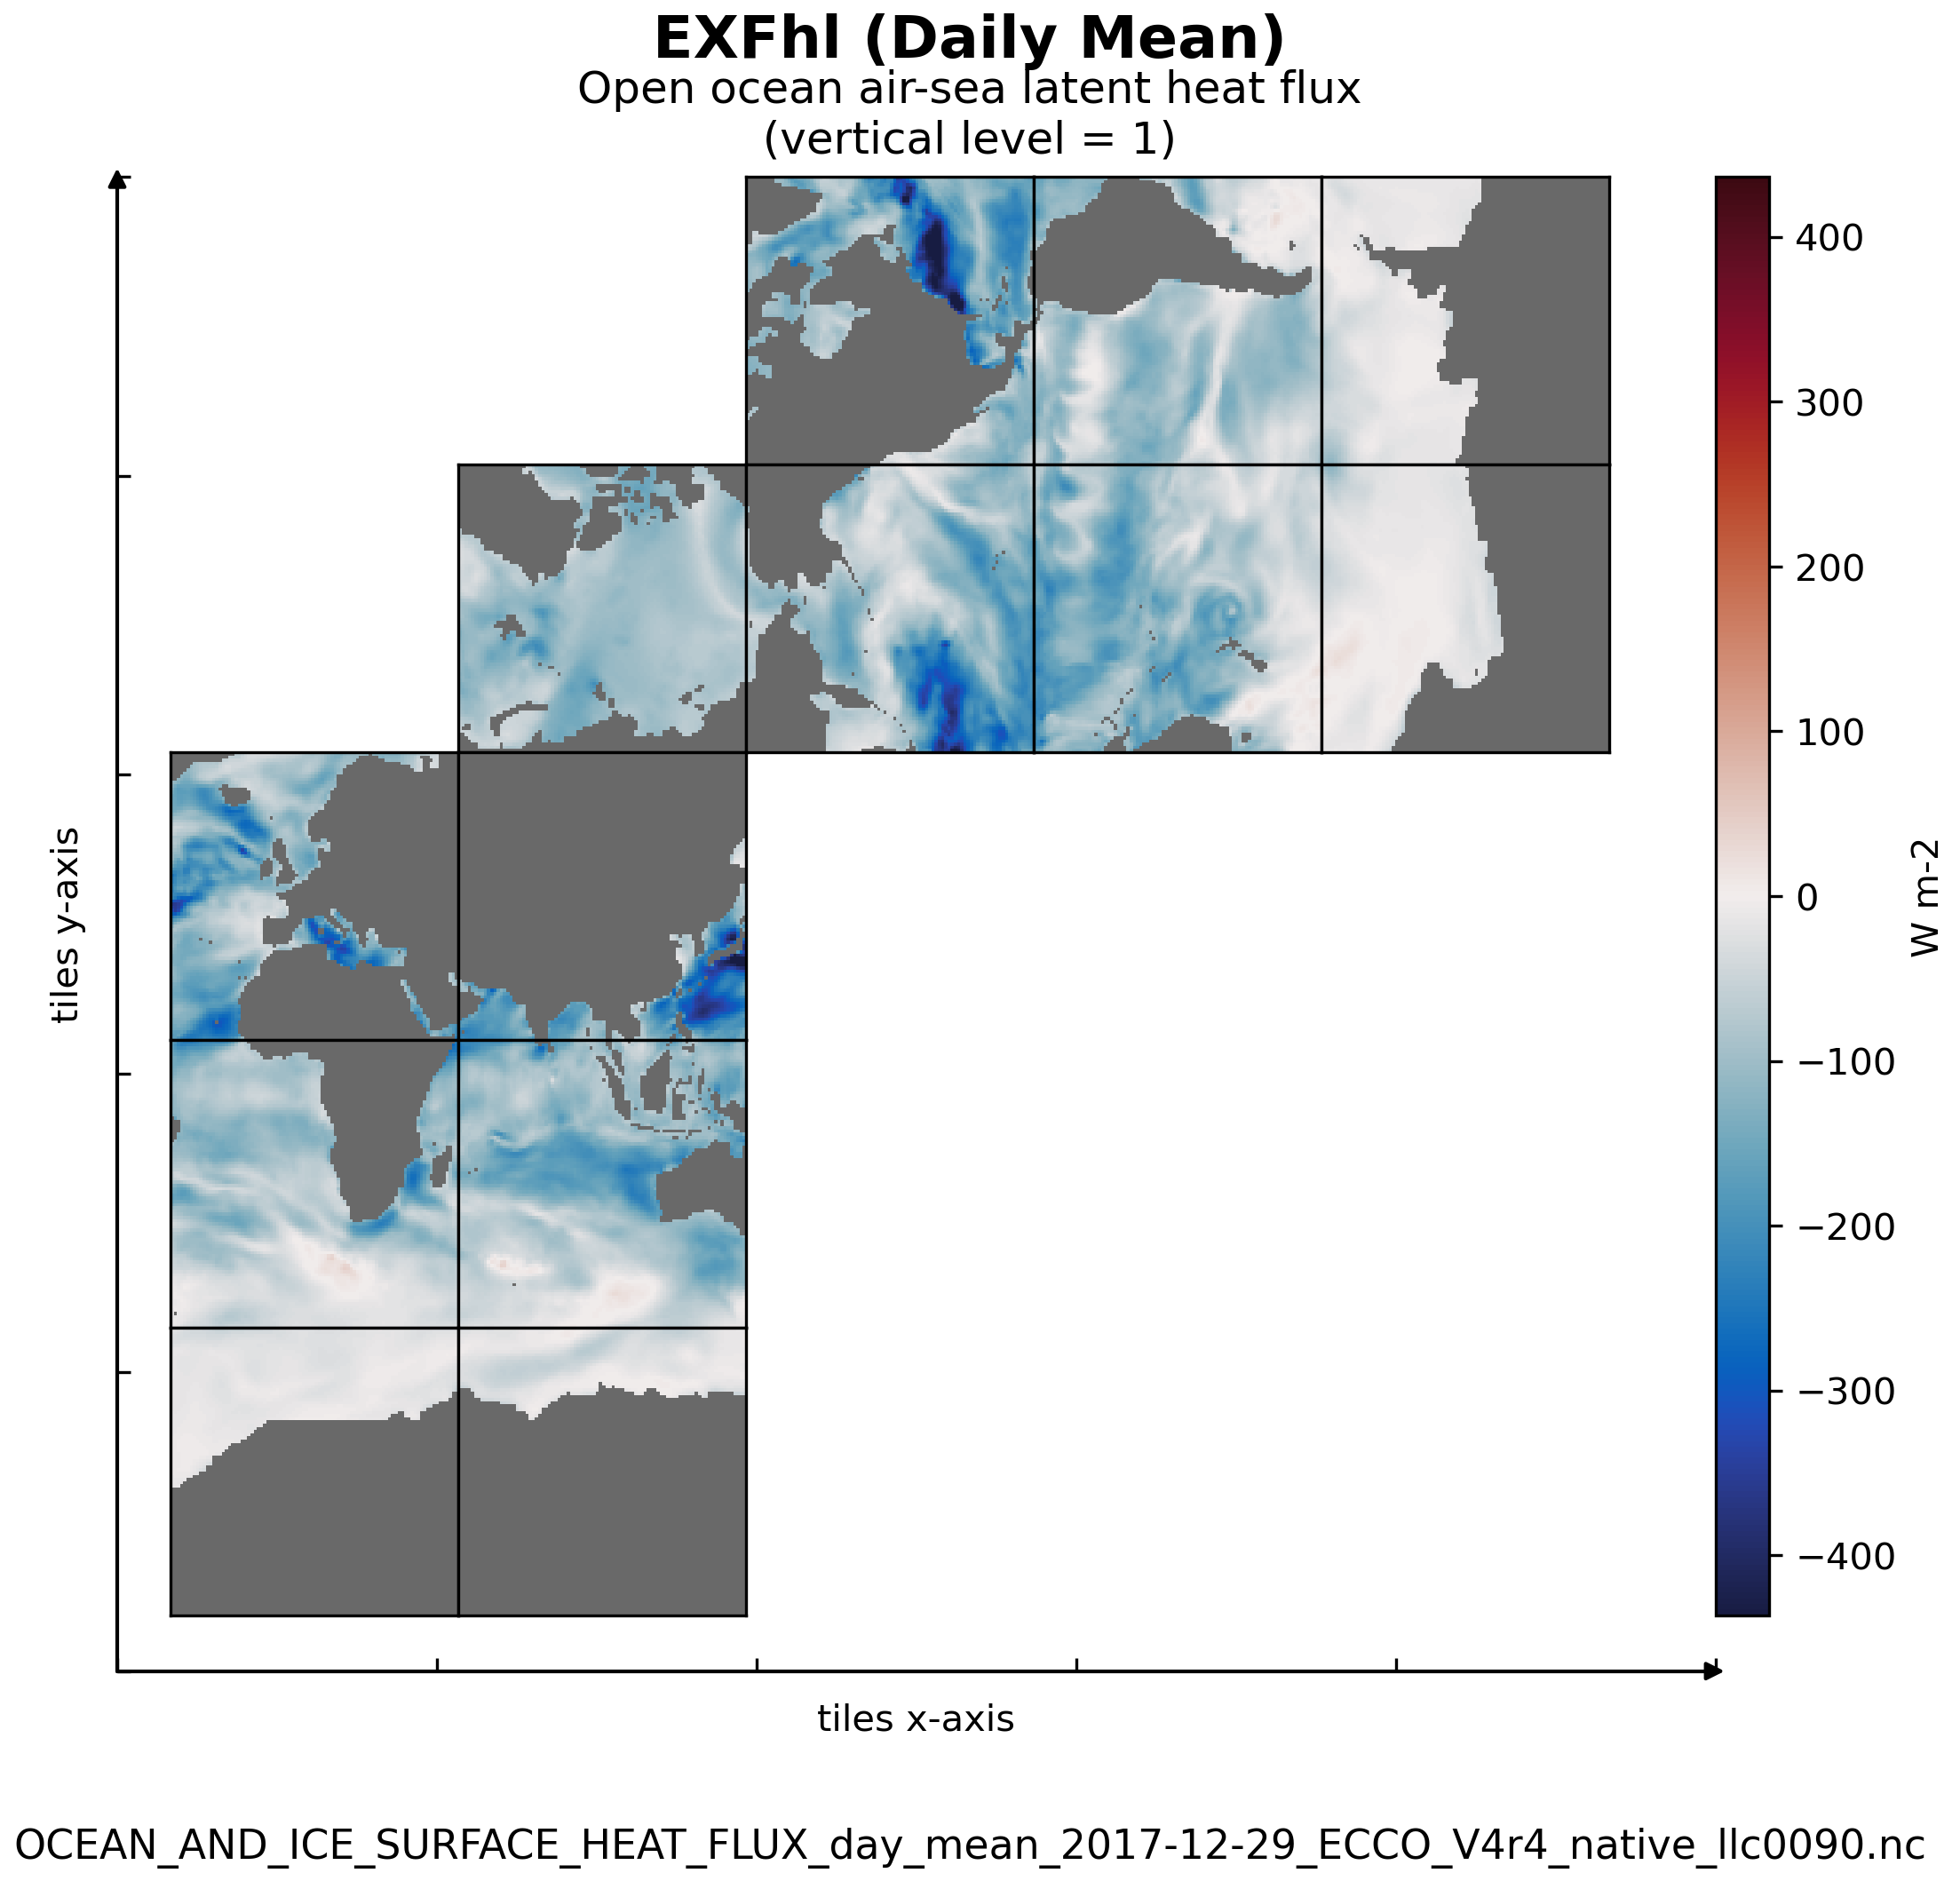
\includegraphics[scale=0.55]{../images/plots/v4r4/native_plots/Ocean_and_Sea-Ice_Surface_Heat_Fluxes/EXFhl.png}
\caption{Dataset: OCEAN\_AND\_ICE\_SURFACE\_HEAT\_FLUX, Variable: EXFhl}
\label{tab:table-OCEAN_AND_ICE_SURFACE_HEAT_FLUX_EXFhl-Plot}
\end{figure}
\newpage
\pagebreak
\subsubsection{Native Variable: EXFhs}
\begin{longtable}{|m{0.06\textwidth}|m{0.3\textwidth}|m{0.45\textwidth}|m{0.12\textwidth}|}
\caption{Attributes description of the variable 'EXFhs' from OCEAN\_AND\_ICE\_SURFACE\_HEAT\_FLUX's  dataset.}
\label{tab:table-OCEAN_AND_ICE_SURFACE_HEAT_FLUX_EXFhs} \\ 
\hline \endhead \hline \endfoot
\rowcolor{lightgray} \textbf{Storage Type} & \textbf{Variable Name} & \textbf{Description} & \textbf{Unit} \\ \hline
float32 & EXFhs & Open ocean air-sea sensible heat flux & W m-2 \\ \hline
\multicolumn{4}{|c|}{\cellcolor{lightgray}{\textbf{Description of the variable in Common Data language (CDL)}}} \\ \hline
\multicolumn{4}{|c|}{\fontfamily{lmtt}\selectfont{\makecell{\parbox{.95\textwidth}{\vspace*{0.25cm} \footnotesize{float32 EXFhs(time, tile, j, i)\\
\hspace*{0.5cm}EXFhs: \_FillValue = 9.96921e+36\\
\hspace*{0.5cm}EXFhs: coordinates = XC time YC\\
\hspace*{0.5cm}EXFhs: coverage\_content\_type = modelResult\\
\hspace*{0.5cm}EXFhs: direction = >0 increases potential temperature (THETA)\\
\hspace*{0.5cm}EXFhs: long\_name = Open ocean air-sea sensible heat flux\\
\hspace*{0.5cm}EXFhs: standard\_name = surface downward sensible heat flux\\
\hspace*{0.5cm}EXFhs: units = W m-2\\
\hspace*{0.5cm}EXFhs: valid\_max = 362.8300476074219\\
\hspace*{0.5cm}EXFhs: valid\_min = -2478.766357421875\\
}}}}} \\ \hline
\rowcolor{lightgray} \multicolumn{4}{|c|}{\textbf{Comments}} \\ \hline
\multicolumn{4}{|p{1\textwidth}|}{\footnotesize{{Air-sea sensible heat flux per unit area of open water (not covered by sea-ice). note: calculated from the bulk formula following large and yeager (2004) ncar/tn-460+str.}}} \\ \hline
\end{longtable}

\begin{figure}[H]
\centering
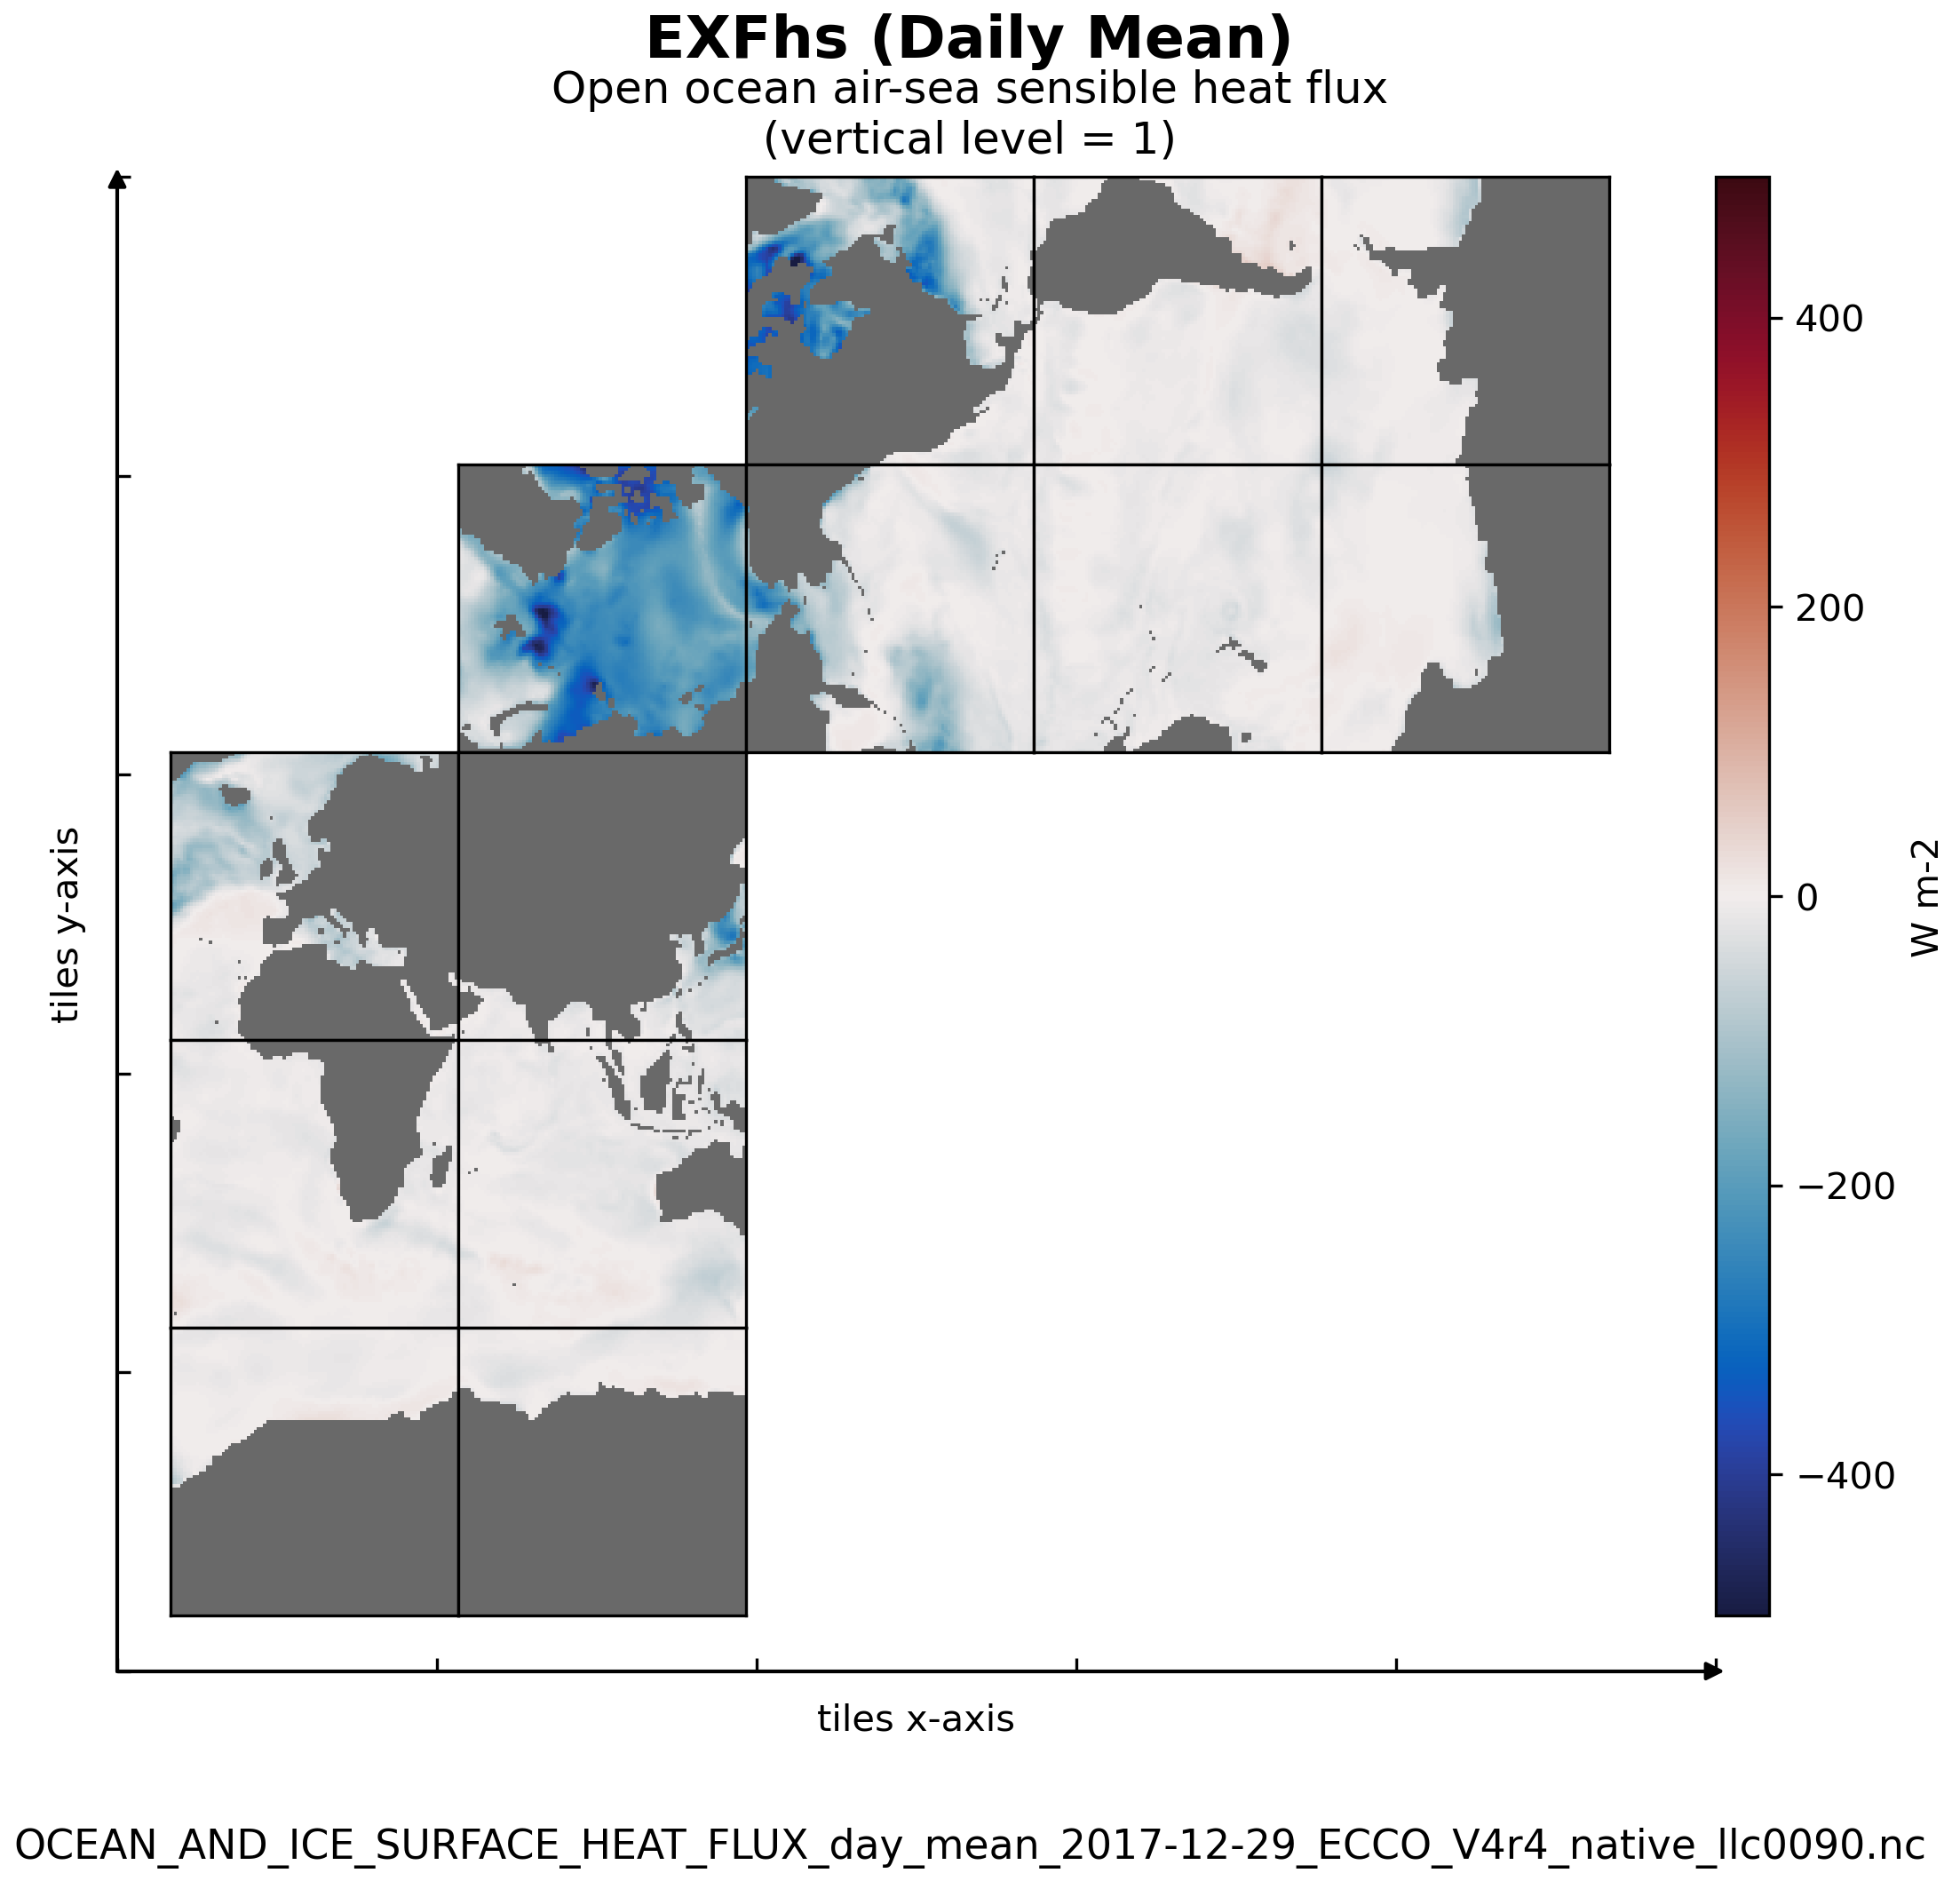
\includegraphics[scale=0.55]{../images/plots/v4r4/native_plots/Ocean_and_Sea-Ice_Surface_Heat_Fluxes/EXFhs.png}
\caption{Dataset: OCEAN\_AND\_ICE\_SURFACE\_HEAT\_FLUX, Variable: EXFhs}
\label{tab:table-OCEAN_AND_ICE_SURFACE_HEAT_FLUX_EXFhs-Plot}
\end{figure}
\newpage
\pagebreak
\subsubsection{Native Variable: EXFlwdn}
\begin{longtable}{|m{0.06\textwidth}|m{0.3\textwidth}|m{0.45\textwidth}|m{0.12\textwidth}|}
\caption{Attributes description of the variable 'EXFlwdn' from OCEAN\_AND\_ICE\_SURFACE\_HEAT\_FLUX's  dataset.}
\label{tab:table-OCEAN_AND_ICE_SURFACE_HEAT_FLUX_EXFlwdn} \\ 
\hline \endhead \hline \endfoot
\rowcolor{lightgray} \textbf{Storage Type} & \textbf{Variable Name} & \textbf{Description} & \textbf{Unit} \\ \hline
float32 & EXFlwdn & Downward longwave radiative flux & W m-2 \\ \hline
\multicolumn{4}{|c|}{\cellcolor{lightgray}{\textbf{Description of the variable in Common Data language (CDL)}}} \\ \hline
\multicolumn{4}{|c|}{\fontfamily{lmtt}\selectfont{\makecell{\parbox{.95\textwidth}{\vspace*{0.25cm} \footnotesize{float32 EXFlwdn(time, tile, j, i)\\
\hspace*{0.5cm}EXFlwdn: \_FillValue = 9.96921e+36\\
\hspace*{0.5cm}EXFlwdn: coordinates = XC time YC\\
\hspace*{0.5cm}EXFlwdn: coverage\_content\_type = modelResult\\
\hspace*{0.5cm}EXFlwdn: direction = >0 increases potential temperature (THETA)\\
\hspace*{0.5cm}EXFlwdn: long\_name = Downward longwave radiative flux\\
\hspace*{0.5cm}EXFlwdn: standard\_name = surface downwelling longwave flux in air\\
\hspace*{0.5cm}EXFlwdn: units = W m-2\\
\hspace*{0.5cm}EXFlwdn: valid\_max = 513.3919067382812\\
\hspace*{0.5cm}EXFlwdn: valid\_min = 4.188045501708984\\
}}}}} \\ \hline
\rowcolor{lightgray} \multicolumn{4}{|c|}{\textbf{Comments}} \\ \hline
\multicolumn{4}{|p{1\textwidth}|}{\footnotesize{{Downward longwave radiative flux. note: sum of era-interim downward longwave radiation and the control adjustment from ocean state estimation.}}} \\ \hline
\end{longtable}

\begin{figure}[H]
\centering
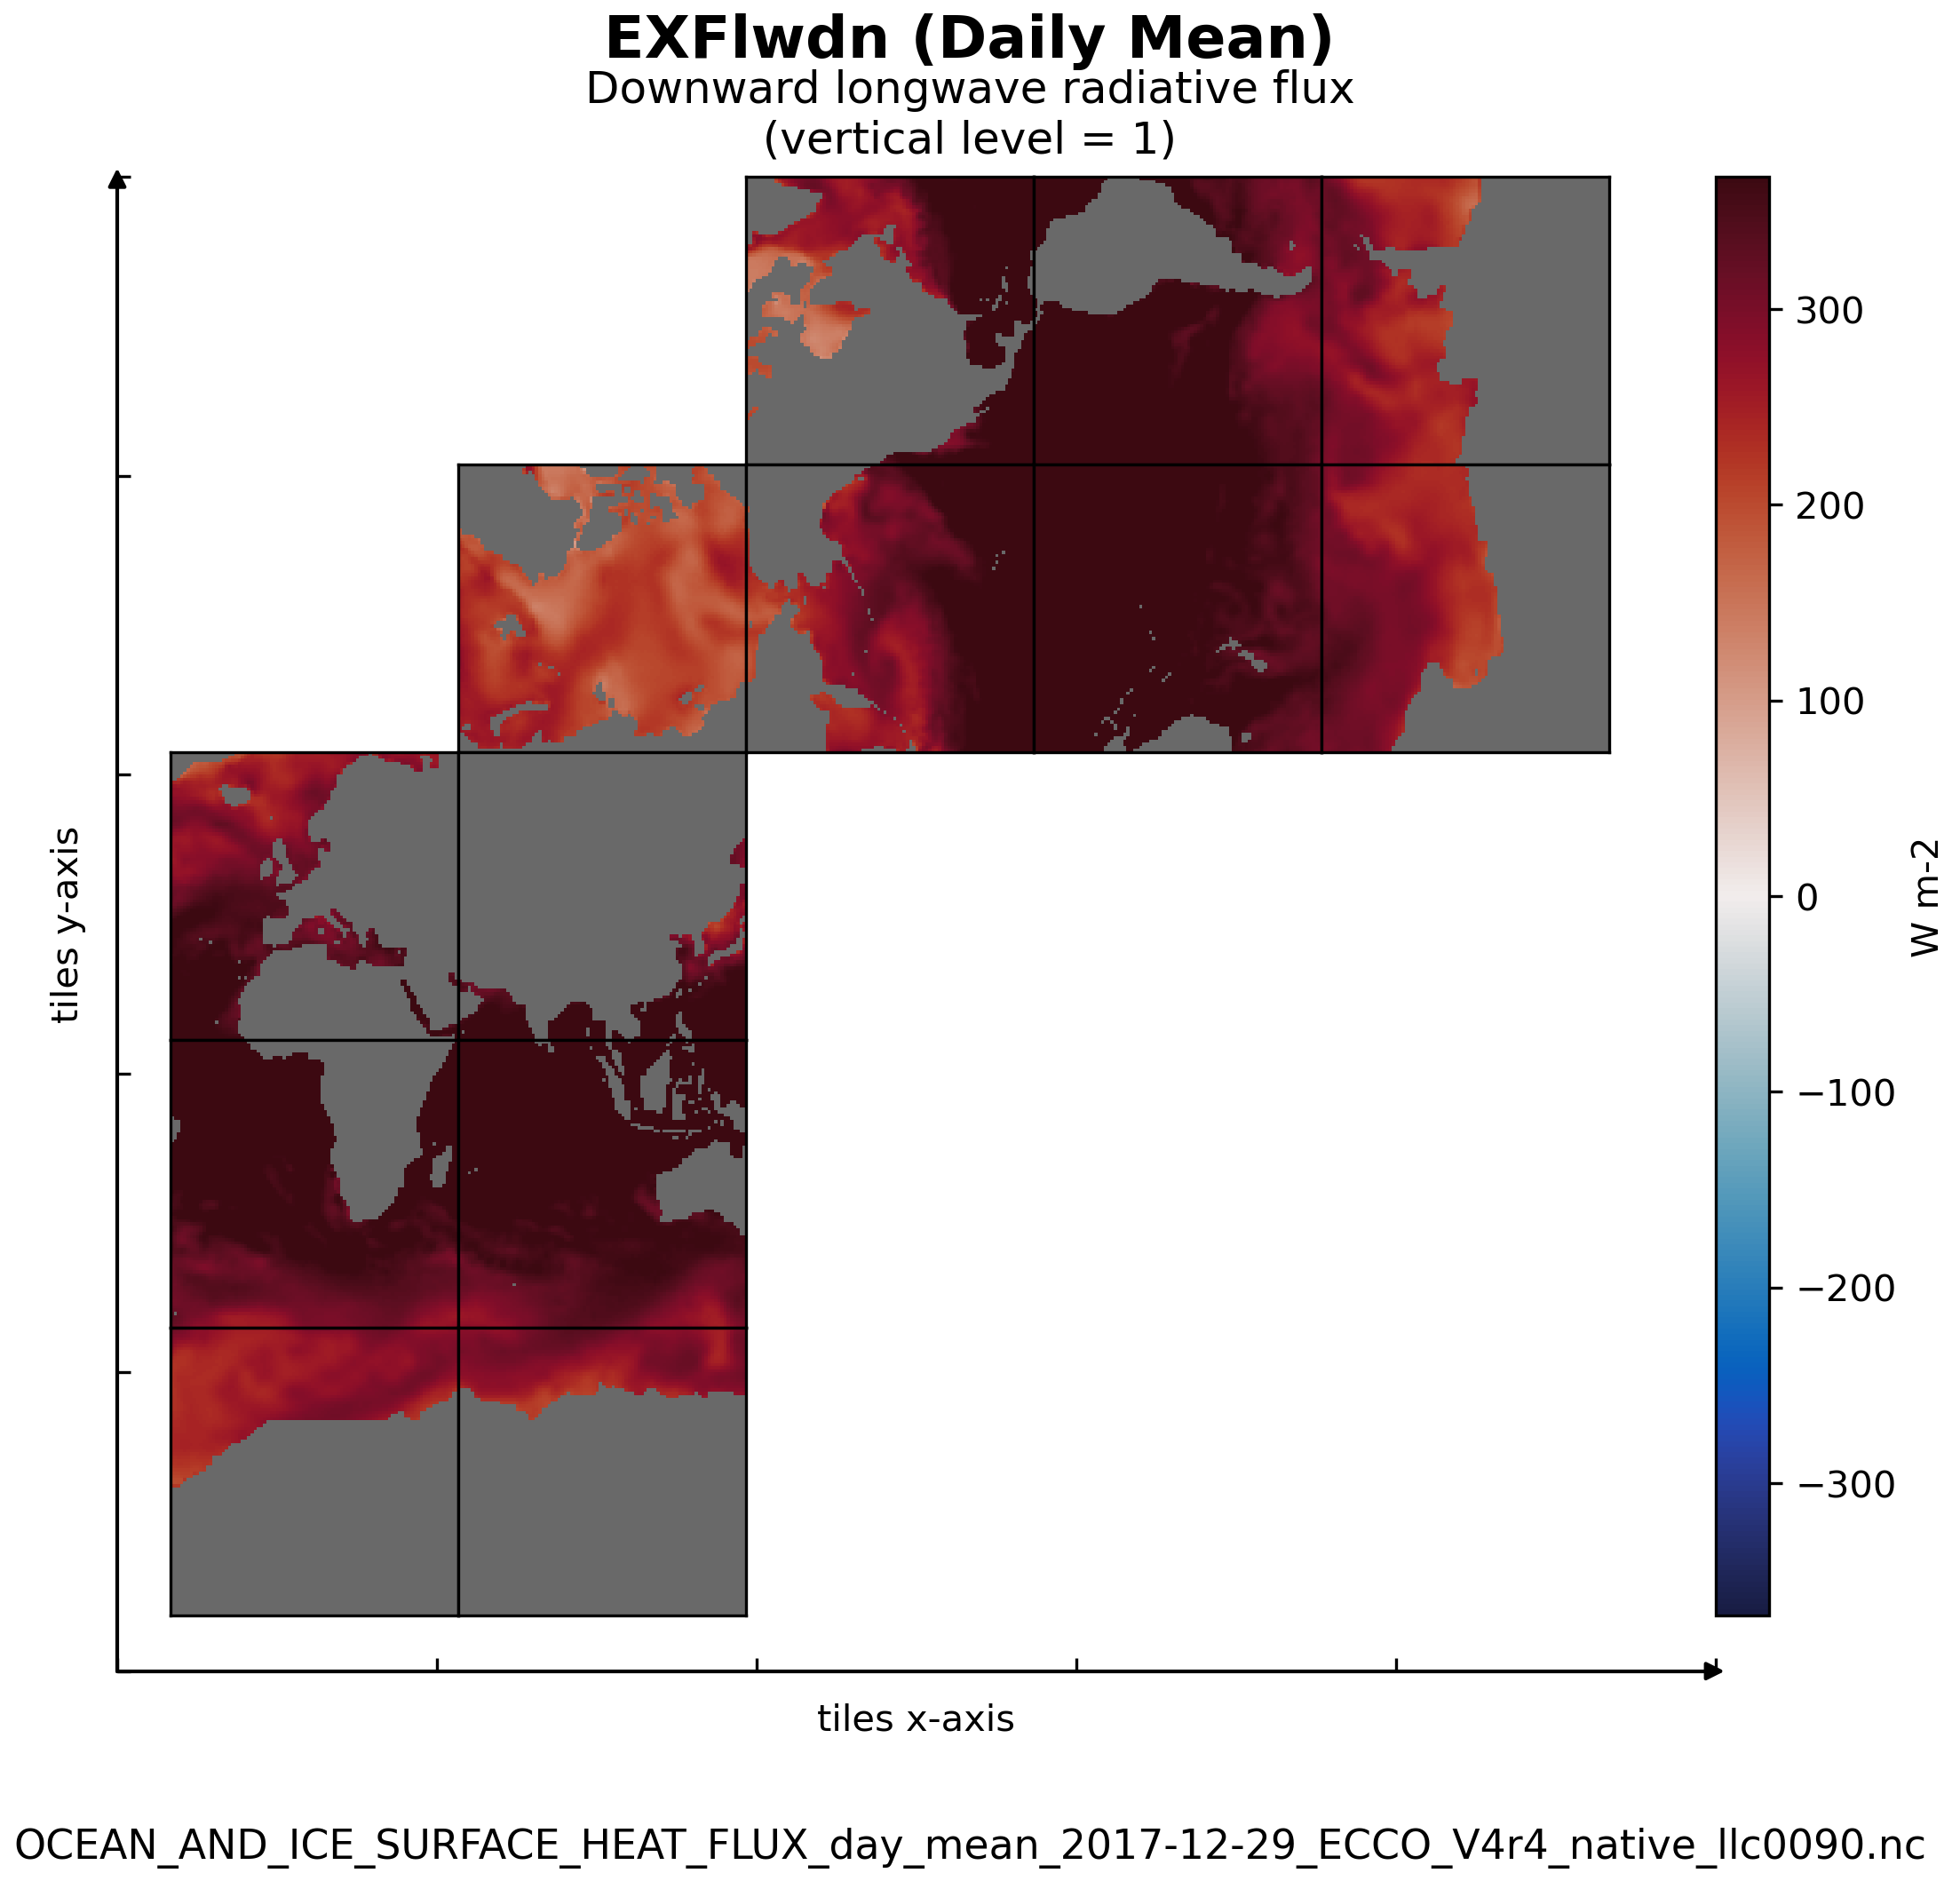
\includegraphics[scale=0.55]{../images/plots/v4r4/native_plots/Ocean_and_Sea-Ice_Surface_Heat_Fluxes/EXFlwdn.png}
\caption{Dataset: OCEAN\_AND\_ICE\_SURFACE\_HEAT\_FLUX, Variable: EXFlwdn}
\label{tab:table-OCEAN_AND_ICE_SURFACE_HEAT_FLUX_EXFlwdn-Plot}
\end{figure}
\newpage
\pagebreak
\subsubsection{Native Variable: EXFlwnet}
\begin{longtable}{|m{0.06\textwidth}|m{0.3\textwidth}|m{0.45\textwidth}|m{0.12\textwidth}|}
\caption{Attributes description of the variable 'EXFlwnet' from OCEAN\_AND\_ICE\_SURFACE\_HEAT\_FLUX's  dataset.}
\label{tab:table-OCEAN_AND_ICE_SURFACE_HEAT_FLUX_EXFlwnet} \\ 
\hline \endhead \hline \endfoot
\rowcolor{lightgray} \textbf{Storage Type} & \textbf{Variable Name} & \textbf{Description} & \textbf{Unit} \\ \hline
float32 & EXFlwnet & Net open ocean longwave radiative flux & W m-2 \\ \hline
\multicolumn{4}{|c|}{\cellcolor{lightgray}{\textbf{Description of the variable in Common Data language (CDL)}}} \\ \hline
\multicolumn{4}{|c|}{\fontfamily{lmtt}\selectfont{\makecell{\parbox{.95\textwidth}{\vspace*{0.25cm} \footnotesize{float32 EXFlwnet(time, tile, j, i)\\
\hspace*{0.5cm}EXFlwnet: \_FillValue = 9.96921e+36\\
\hspace*{0.5cm}EXFlwnet: coordinates = XC time YC\\
\hspace*{0.5cm}EXFlwnet: coverage\_content\_type = modelResult\\
\hspace*{0.5cm}EXFlwnet: direction = >0 increases potential temperature (THETA)\\
\hspace*{0.5cm}EXFlwnet: long\_name = Net open ocean longwave radiative flux\\
\hspace*{0.5cm}EXFlwnet: standard\_name = surface net downward longwave flux\\
\hspace*{0.5cm}EXFlwnet: units = W m-2\\
\hspace*{0.5cm}EXFlwnet: valid\_max = 293.4114990234375\\
\hspace*{0.5cm}EXFlwnet: valid\_min = -144.3661346435547\\
}}}}} \\ \hline
\rowcolor{lightgray} \multicolumn{4}{|c|}{\textbf{Comments}} \\ \hline
\multicolumn{4}{|p{1\textwidth}|}{\footnotesize{{Net longwave radiative flux per unit area of open water (not covered by sea-ice). note: net longwave radiation over open water calculated from downward longwave radiation (exflwdn) and upward longwave radiation from ocean and sea-ice thermal emission (stefan-boltzman law).}}} \\ \hline
\end{longtable}

\begin{figure}[H]
\centering
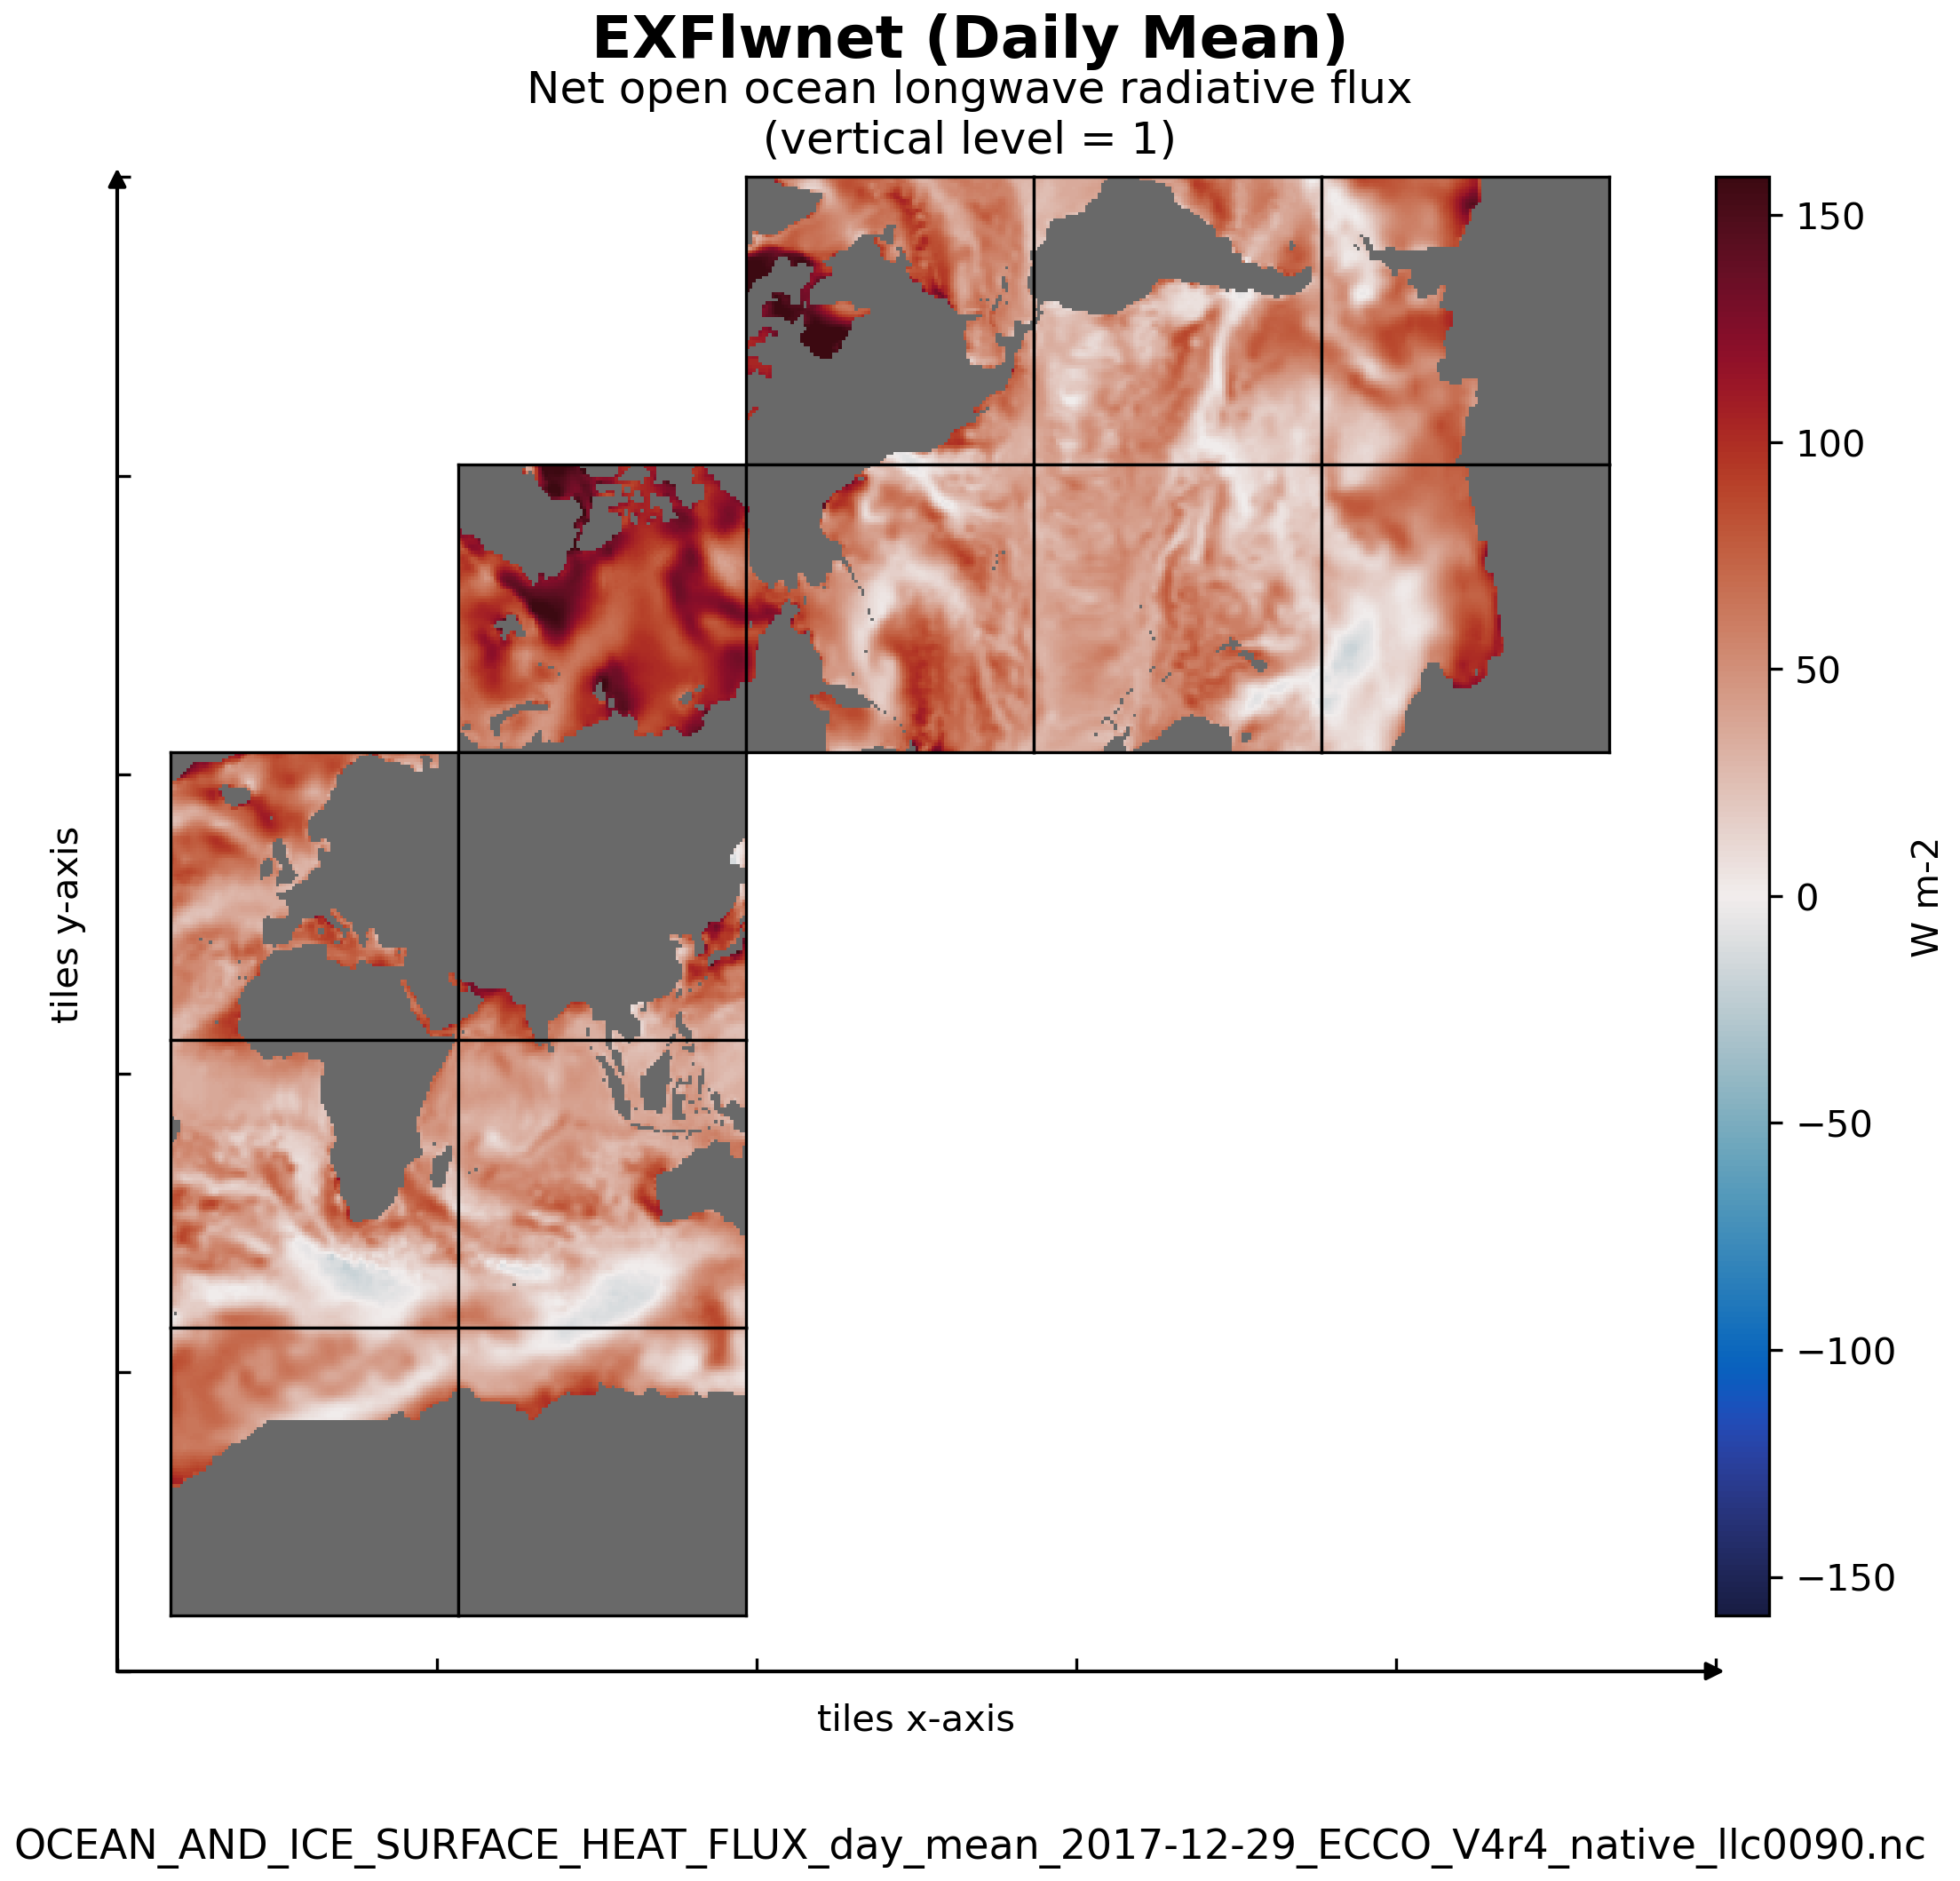
\includegraphics[scale=0.55]{../images/plots/v4r4/native_plots/Ocean_and_Sea-Ice_Surface_Heat_Fluxes/EXFlwnet.png}
\caption{Dataset: OCEAN\_AND\_ICE\_SURFACE\_HEAT\_FLUX, Variable: EXFlwnet}
\label{tab:table-OCEAN_AND_ICE_SURFACE_HEAT_FLUX_EXFlwnet-Plot}
\end{figure}
\newpage
\pagebreak
\subsubsection{Native Variable: EXFqnet}
\begin{longtable}{|m{0.06\textwidth}|m{0.3\textwidth}|m{0.45\textwidth}|m{0.12\textwidth}|}
\caption{Attributes description of the variable 'EXFqnet' from OCEAN\_AND\_ICE\_SURFACE\_HEAT\_FLUX's  dataset.}
\label{tab:table-OCEAN_AND_ICE_SURFACE_HEAT_FLUX_EXFqnet} \\ 
\hline \endhead \hline \endfoot
\rowcolor{lightgray} \textbf{Storage Type} & \textbf{Variable Name} & \textbf{Description} & \textbf{Unit} \\ \hline
float32 & EXFqnet & Open ocean net air-sea heat flux & W m-2 \\ \hline
\multicolumn{4}{|c|}{\cellcolor{lightgray}{\textbf{Description of the variable in Common Data language (CDL)}}} \\ \hline
\multicolumn{4}{|c|}{\fontfamily{lmtt}\selectfont{\makecell{\parbox{.95\textwidth}{\vspace*{0.25cm} \footnotesize{float32 EXFqnet(time, tile, j, i)\\
\hspace*{0.5cm}EXFqnet: \_FillValue = 9.96921e+36\\
\hspace*{0.5cm}EXFqnet: coordinates = XC time YC\\
\hspace*{0.5cm}EXFqnet: coverage\_content\_type = modelResult\\
\hspace*{0.5cm}EXFqnet: direction = >0 increases potential temperature (THETA)\\
\hspace*{0.5cm}EXFqnet: long\_name = Open ocean net air-sea heat flux\\
\hspace*{0.5cm}EXFqnet: units = W m-2\\
\hspace*{0.5cm}EXFqnet: valid\_max = 3408.977783203125\\
\hspace*{0.5cm}EXFqnet: valid\_min = -687.8736572265625\\
}}}}} \\ \hline
\rowcolor{lightgray} \multicolumn{4}{|c|}{\textbf{Comments}} \\ \hline
\multicolumn{4}{|p{1\textwidth}|}{\footnotesize{{Net air-sea heat flux (turbulent and radiative) per unit area of open water (not covered by sea-ice). note: net upward heat flux over open water, calculated as exflwnet+exfswnet-exflh-exfhs.}}} \\ \hline
\end{longtable}

\begin{figure}[H]
\centering
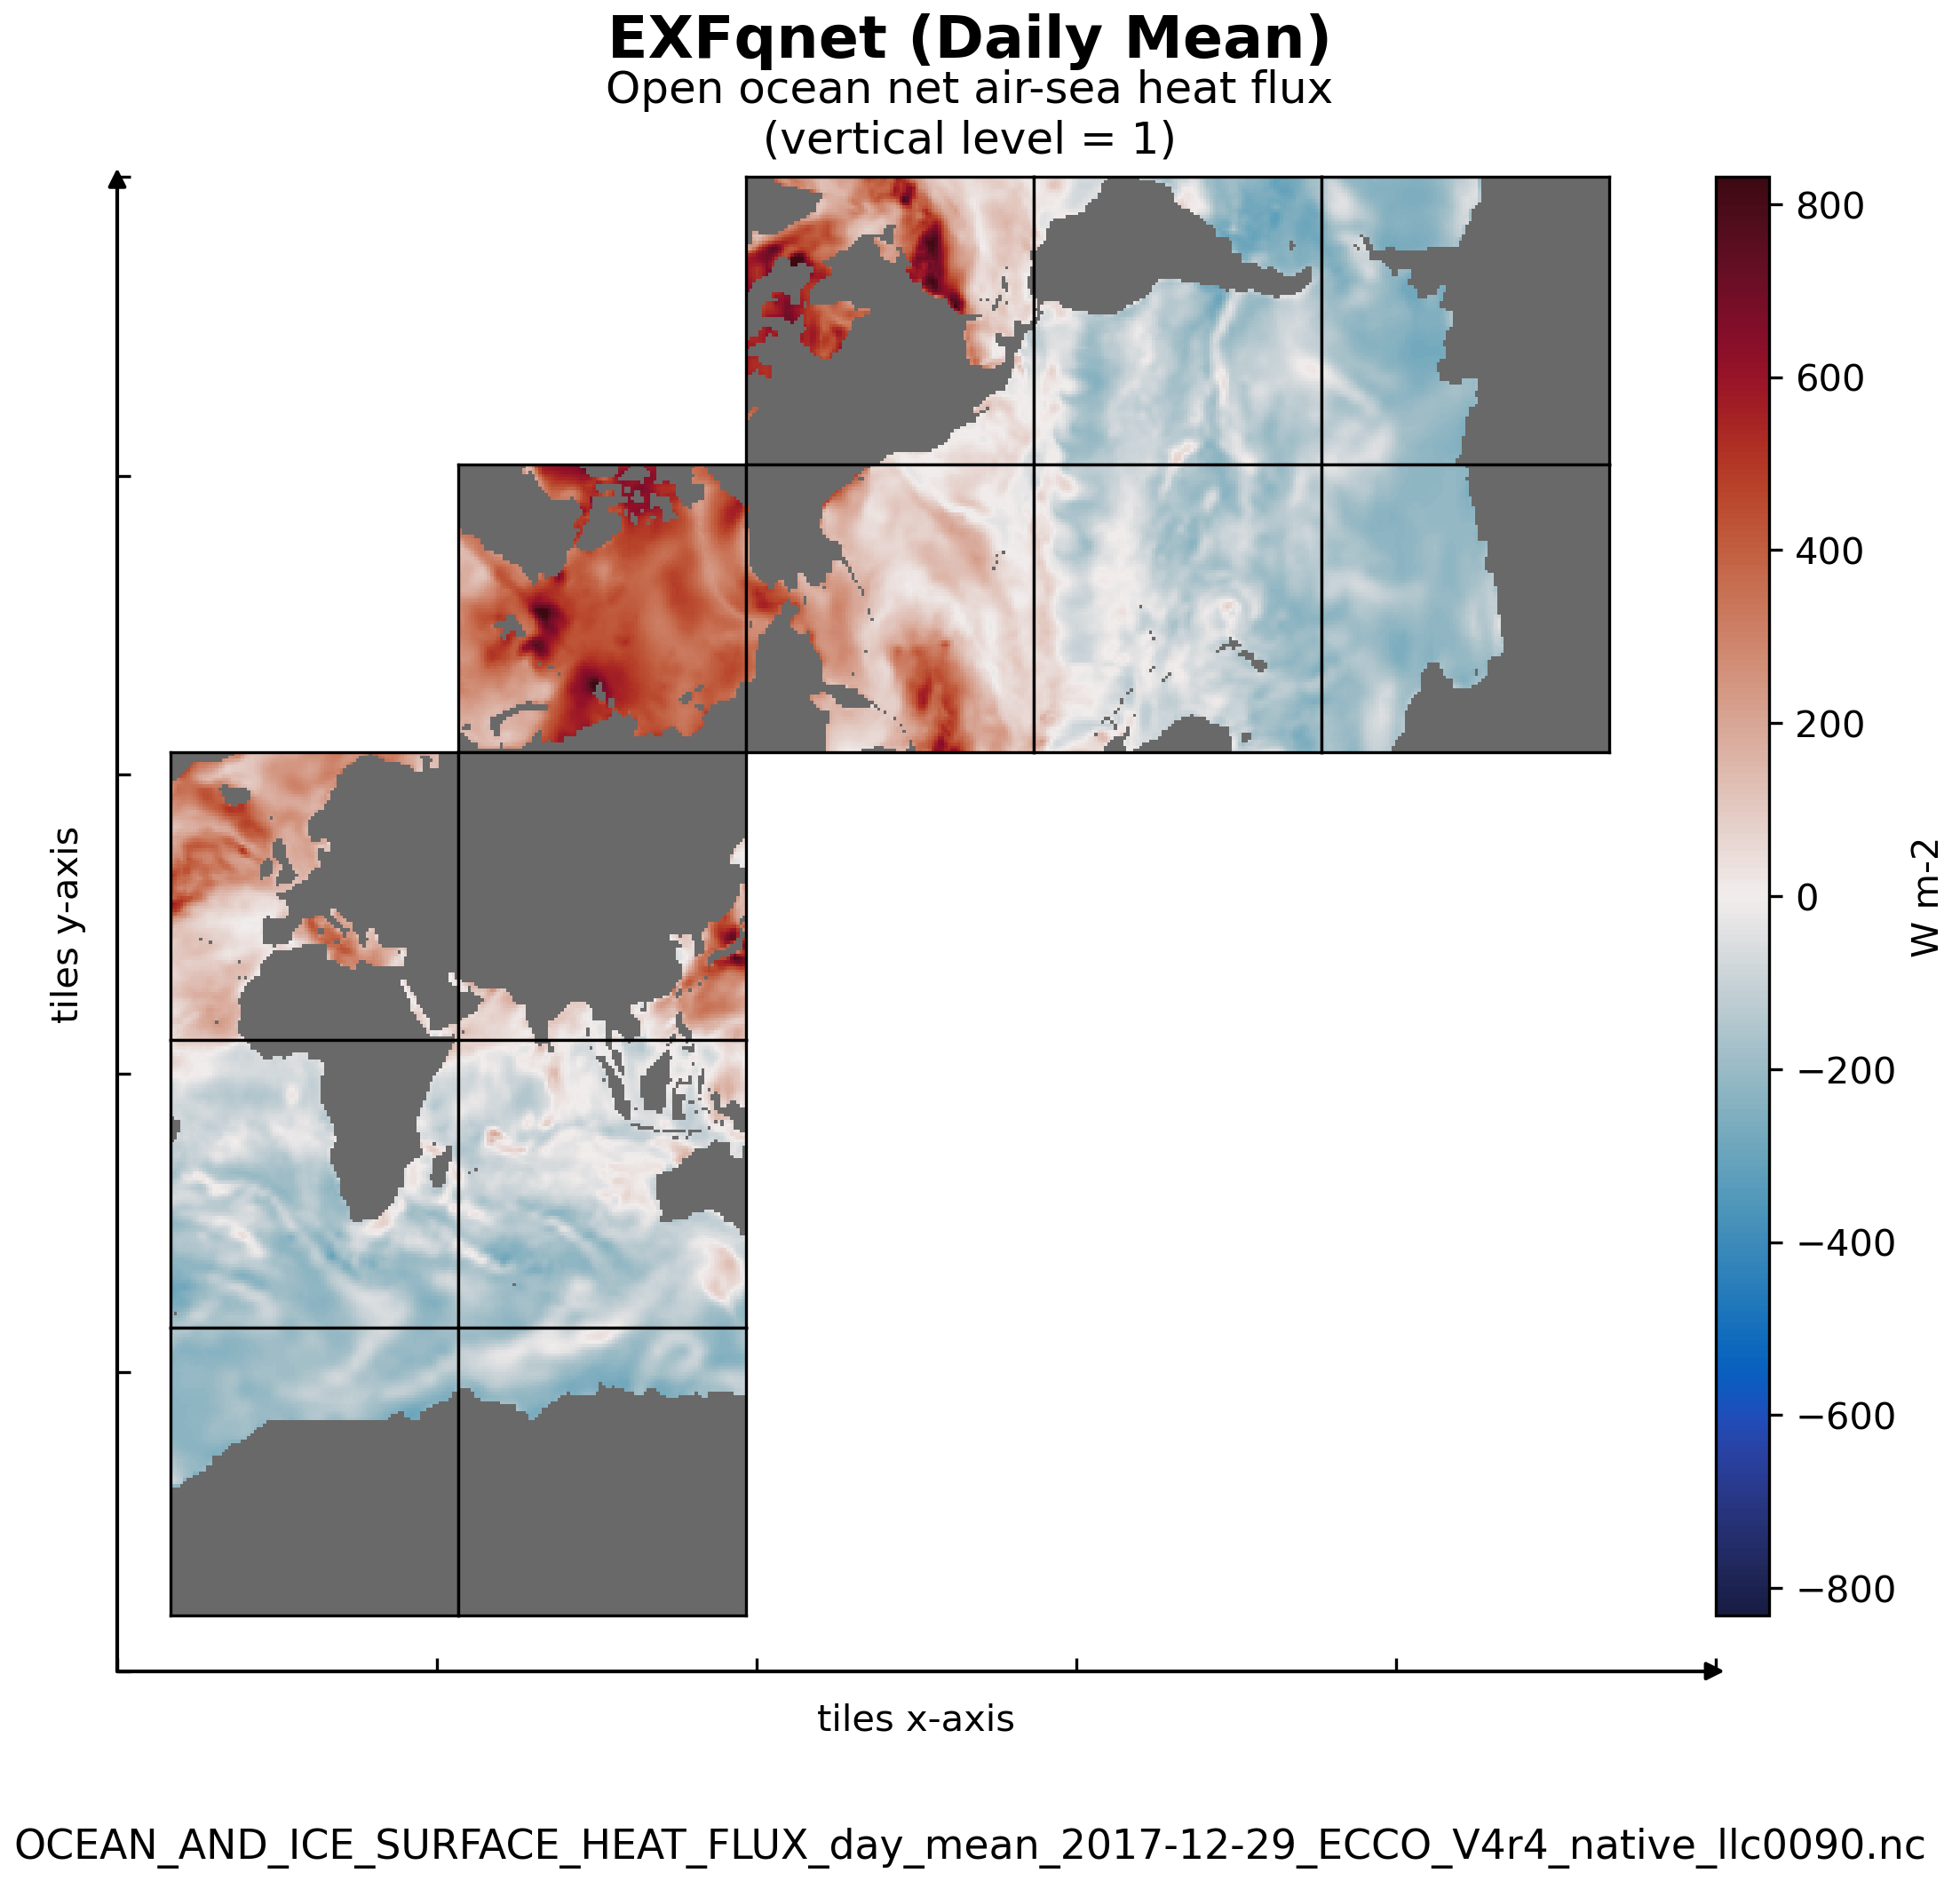
\includegraphics[scale=0.55]{../images/plots/v4r4/native_plots/Ocean_and_Sea-Ice_Surface_Heat_Fluxes/EXFqnet.png}
\caption{Dataset: OCEAN\_AND\_ICE\_SURFACE\_HEAT\_FLUX, Variable: EXFqnet}
\label{tab:table-OCEAN_AND_ICE_SURFACE_HEAT_FLUX_EXFqnet-Plot}
\end{figure}
\newpage
\pagebreak
\subsubsection{Native Variable: EXFswdn}
\begin{longtable}{|m{0.06\textwidth}|m{0.3\textwidth}|m{0.45\textwidth}|m{0.12\textwidth}|}
\caption{Attributes description of the variable 'EXFswdn' from OCEAN\_AND\_ICE\_SURFACE\_HEAT\_FLUX's  dataset.}
\label{tab:table-OCEAN_AND_ICE_SURFACE_HEAT_FLUX_EXFswdn} \\ 
\hline \endhead \hline \endfoot
\rowcolor{lightgray} \textbf{Storage Type} & \textbf{Variable Name} & \textbf{Description} & \textbf{Unit} \\ \hline
float32 & EXFswdn & Downwelling shortwave radiative flux & W m-2 \\ \hline
\multicolumn{4}{|c|}{\cellcolor{lightgray}{\textbf{Description of the variable in Common Data language (CDL)}}} \\ \hline
\multicolumn{4}{|c|}{\fontfamily{lmtt}\selectfont{\makecell{\parbox{.95\textwidth}{\vspace*{0.25cm} \footnotesize{float32 EXFswdn(time, tile, j, i)\\
\hspace*{0.5cm}EXFswdn: \_FillValue = 9.96921e+36\\
\hspace*{0.5cm}EXFswdn: coordinates = XC time YC\\
\hspace*{0.5cm}EXFswdn: coverage\_content\_type = modelResult\\
\hspace*{0.5cm}EXFswdn: direction = >0 increases potential temperature (THETA)\\
\hspace*{0.5cm}EXFswdn: long\_name = Downwelling shortwave radiative flux\\
\hspace*{0.5cm}EXFswdn: standard\_name = surface downwelling shortwave flux in air\\
\hspace*{0.5cm}EXFswdn: units = W m-2\\
\hspace*{0.5cm}EXFswdn: valid\_max = 707.345947265625\\
\hspace*{0.5cm}EXFswdn: valid\_min = -224.63368225097656\\
}}}}} \\ \hline
\rowcolor{lightgray} \multicolumn{4}{|c|}{\textbf{Comments}} \\ \hline
\multicolumn{4}{|p{1\textwidth}|}{\footnotesize{{Downward shortwave radiative flux. note: sum of era-interim downward shortwave radiation and the control adjustment from ocean state estimation.}}} \\ \hline
\end{longtable}

\begin{figure}[H]
\centering
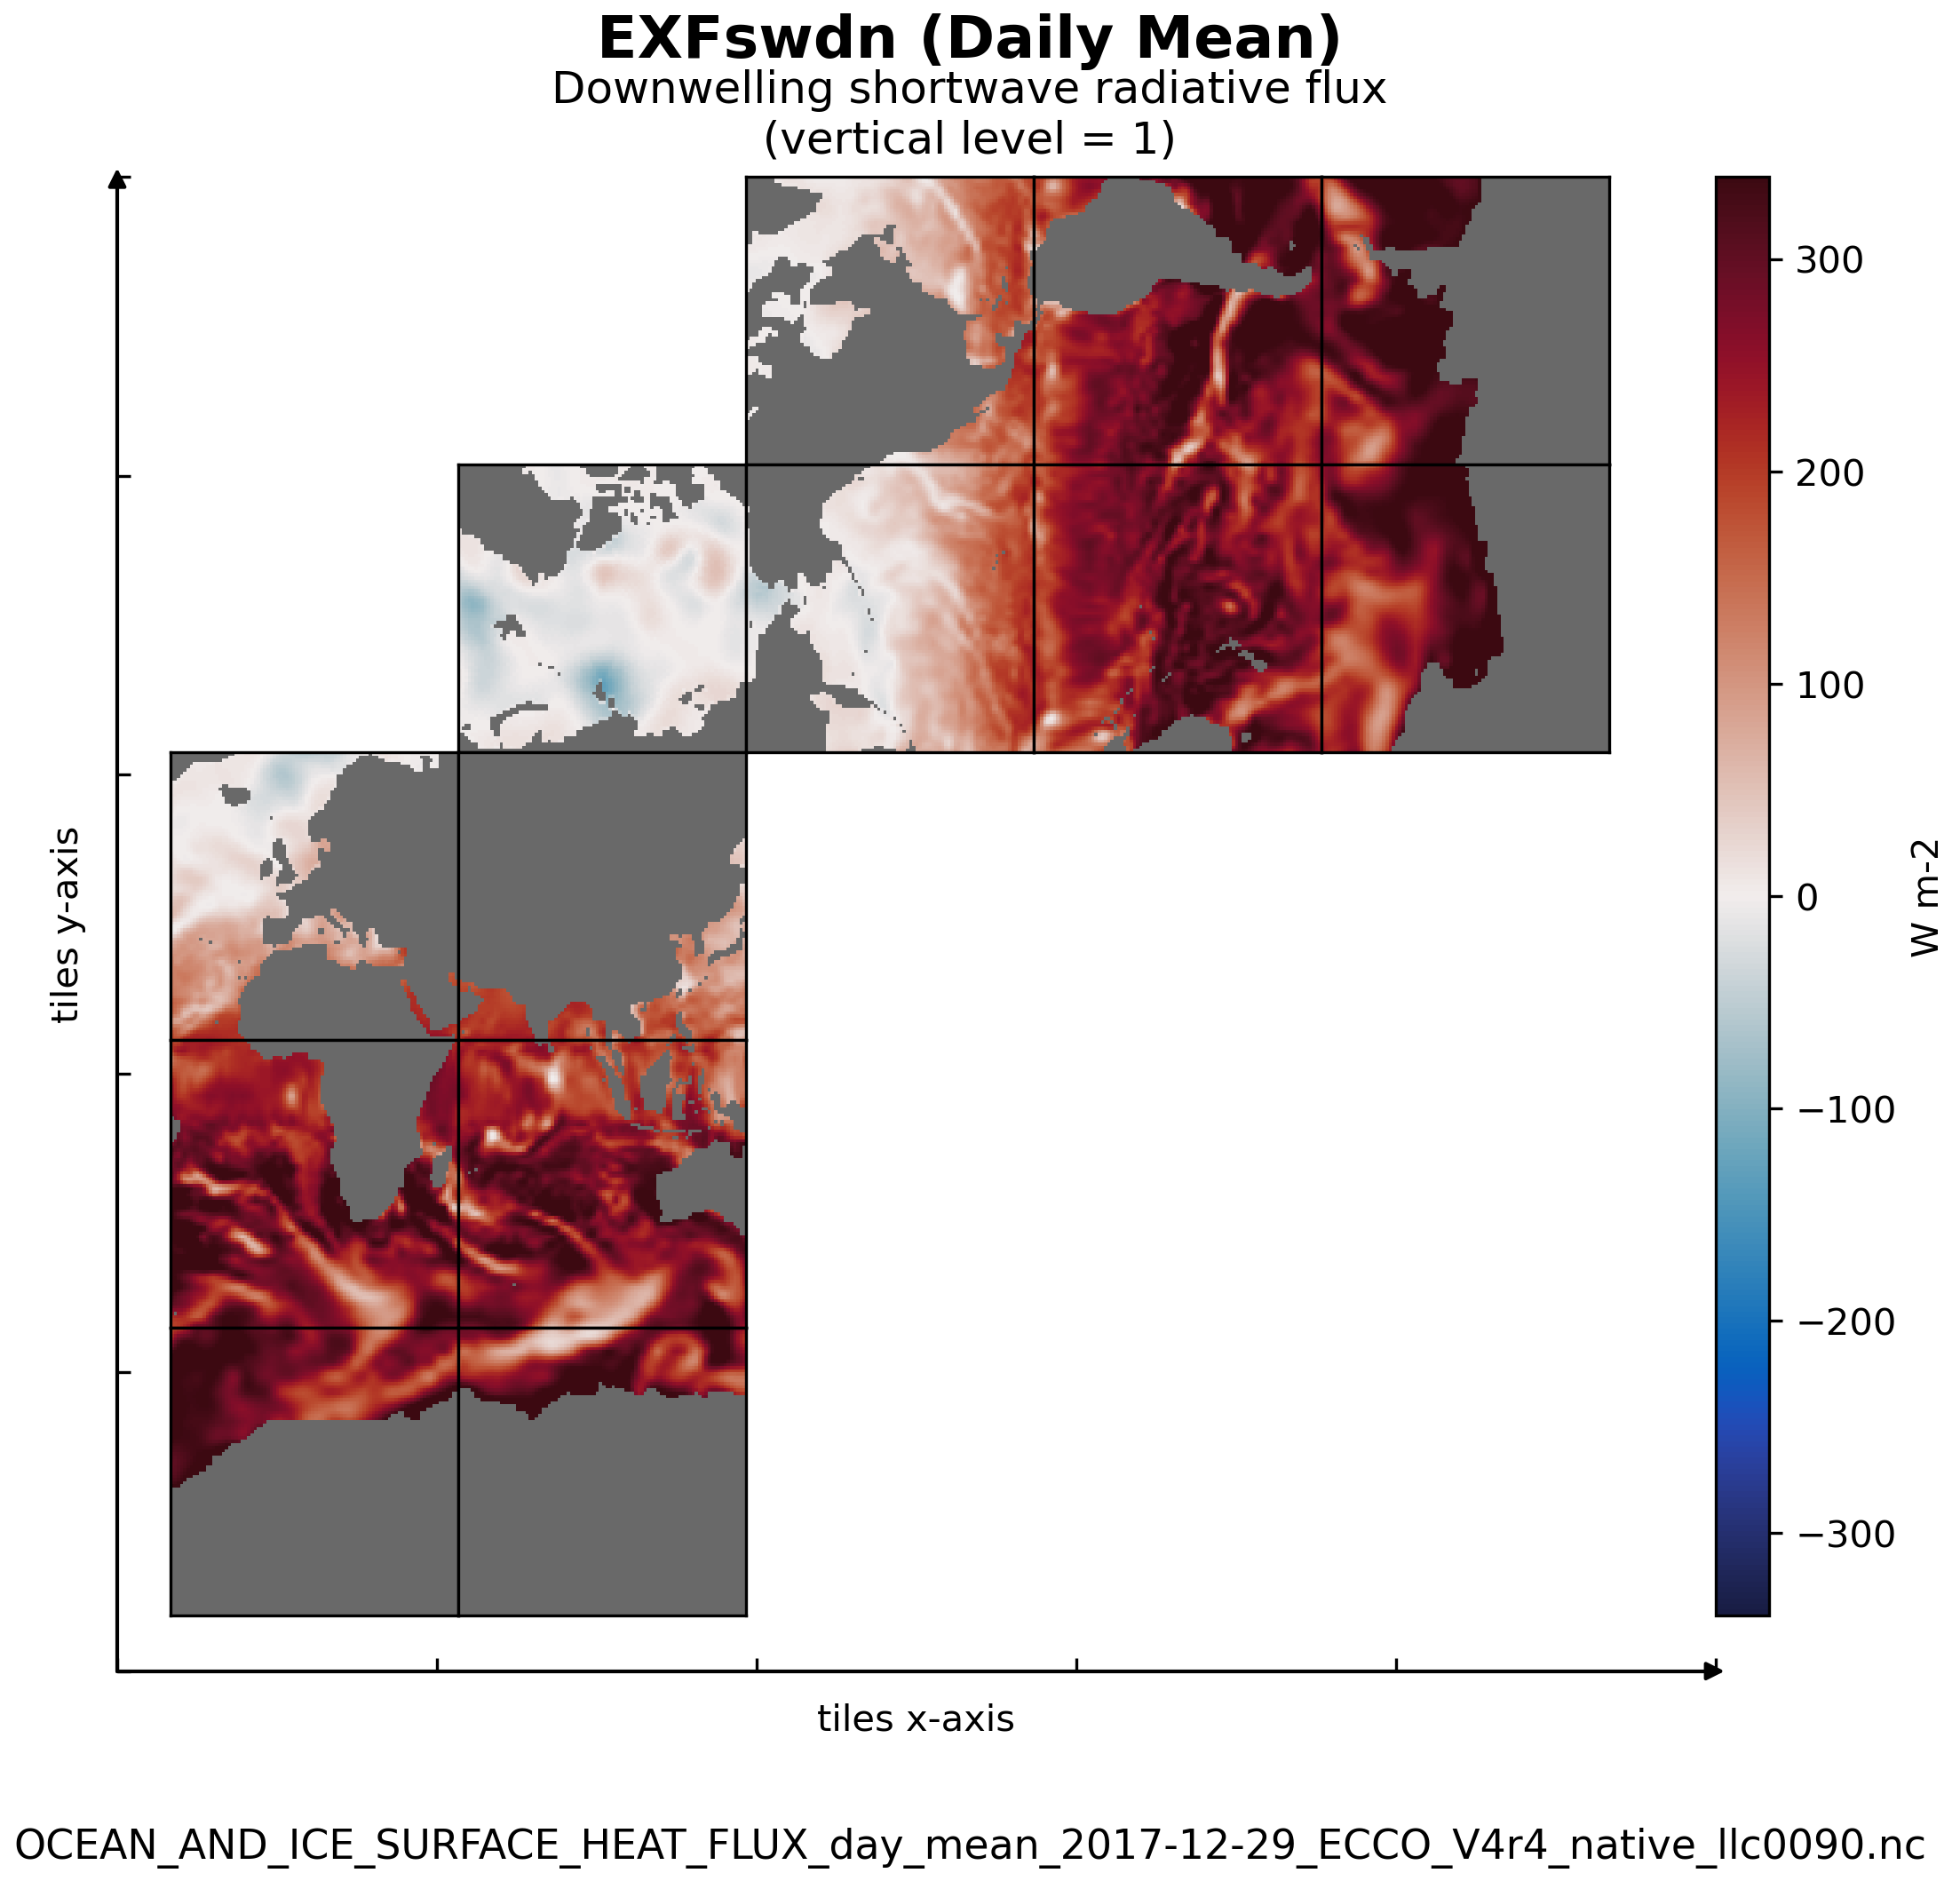
\includegraphics[scale=0.55]{../images/plots/v4r4/native_plots/Ocean_and_Sea-Ice_Surface_Heat_Fluxes/EXFswdn.png}
\caption{Dataset: OCEAN\_AND\_ICE\_SURFACE\_HEAT\_FLUX, Variable: EXFswdn}
\label{tab:table-OCEAN_AND_ICE_SURFACE_HEAT_FLUX_EXFswdn-Plot}
\end{figure}
\newpage
\pagebreak
\subsubsection{Native Variable: EXFswnet}
\begin{longtable}{|m{0.06\textwidth}|m{0.3\textwidth}|m{0.45\textwidth}|m{0.12\textwidth}|}
\caption{Attributes description of the variable 'EXFswnet' from OCEAN\_AND\_ICE\_SURFACE\_HEAT\_FLUX's  dataset.}
\label{tab:table-OCEAN_AND_ICE_SURFACE_HEAT_FLUX_EXFswnet} \\ 
\hline \endhead \hline \endfoot
\rowcolor{lightgray} \textbf{Storage Type} & \textbf{Variable Name} & \textbf{Description} & \textbf{Unit} \\ \hline
float32 & EXFswnet & Open ocean net shortwave radiative flux & W m-2 \\ \hline
\multicolumn{4}{|c|}{\cellcolor{lightgray}{\textbf{Description of the variable in Common Data language (CDL)}}} \\ \hline
\multicolumn{4}{|c|}{\fontfamily{lmtt}\selectfont{\makecell{\parbox{.95\textwidth}{\vspace*{0.25cm} \footnotesize{float32 EXFswnet(time, tile, j, i)\\
\hspace*{0.5cm}EXFswnet: \_FillValue = 9.96921e+36\\
\hspace*{0.5cm}EXFswnet: coordinates = XC time YC\\
\hspace*{0.5cm}EXFswnet: coverage\_content\_type = modelResult\\
\hspace*{0.5cm}EXFswnet: direction = >0 increases potential temperature (THETA)\\
\hspace*{0.5cm}EXFswnet: long\_name = Open ocean net shortwave radiative flux\\
\hspace*{0.5cm}EXFswnet: standard\_name = surface net downward shortwave flux\\
\hspace*{0.5cm}EXFswnet: units = W m-2\\
\hspace*{0.5cm}EXFswnet: valid\_max = 194.18458557128906\\
\hspace*{0.5cm}EXFswnet: valid\_min = -655.6171264648438\\
}}}}} \\ \hline
\rowcolor{lightgray} \multicolumn{4}{|c|}{\textbf{Comments}} \\ \hline
\multicolumn{4}{|p{1\textwidth}|}{\footnotesize{{Net shortwave radiative flux per unit area of open water (not covered by sea-ice). note: net shortwave radiation over open water calculated from downward shortwave flux (exfswdn) and ocean surface albdeo.}}} \\ \hline
\end{longtable}

\begin{figure}[H]
\centering
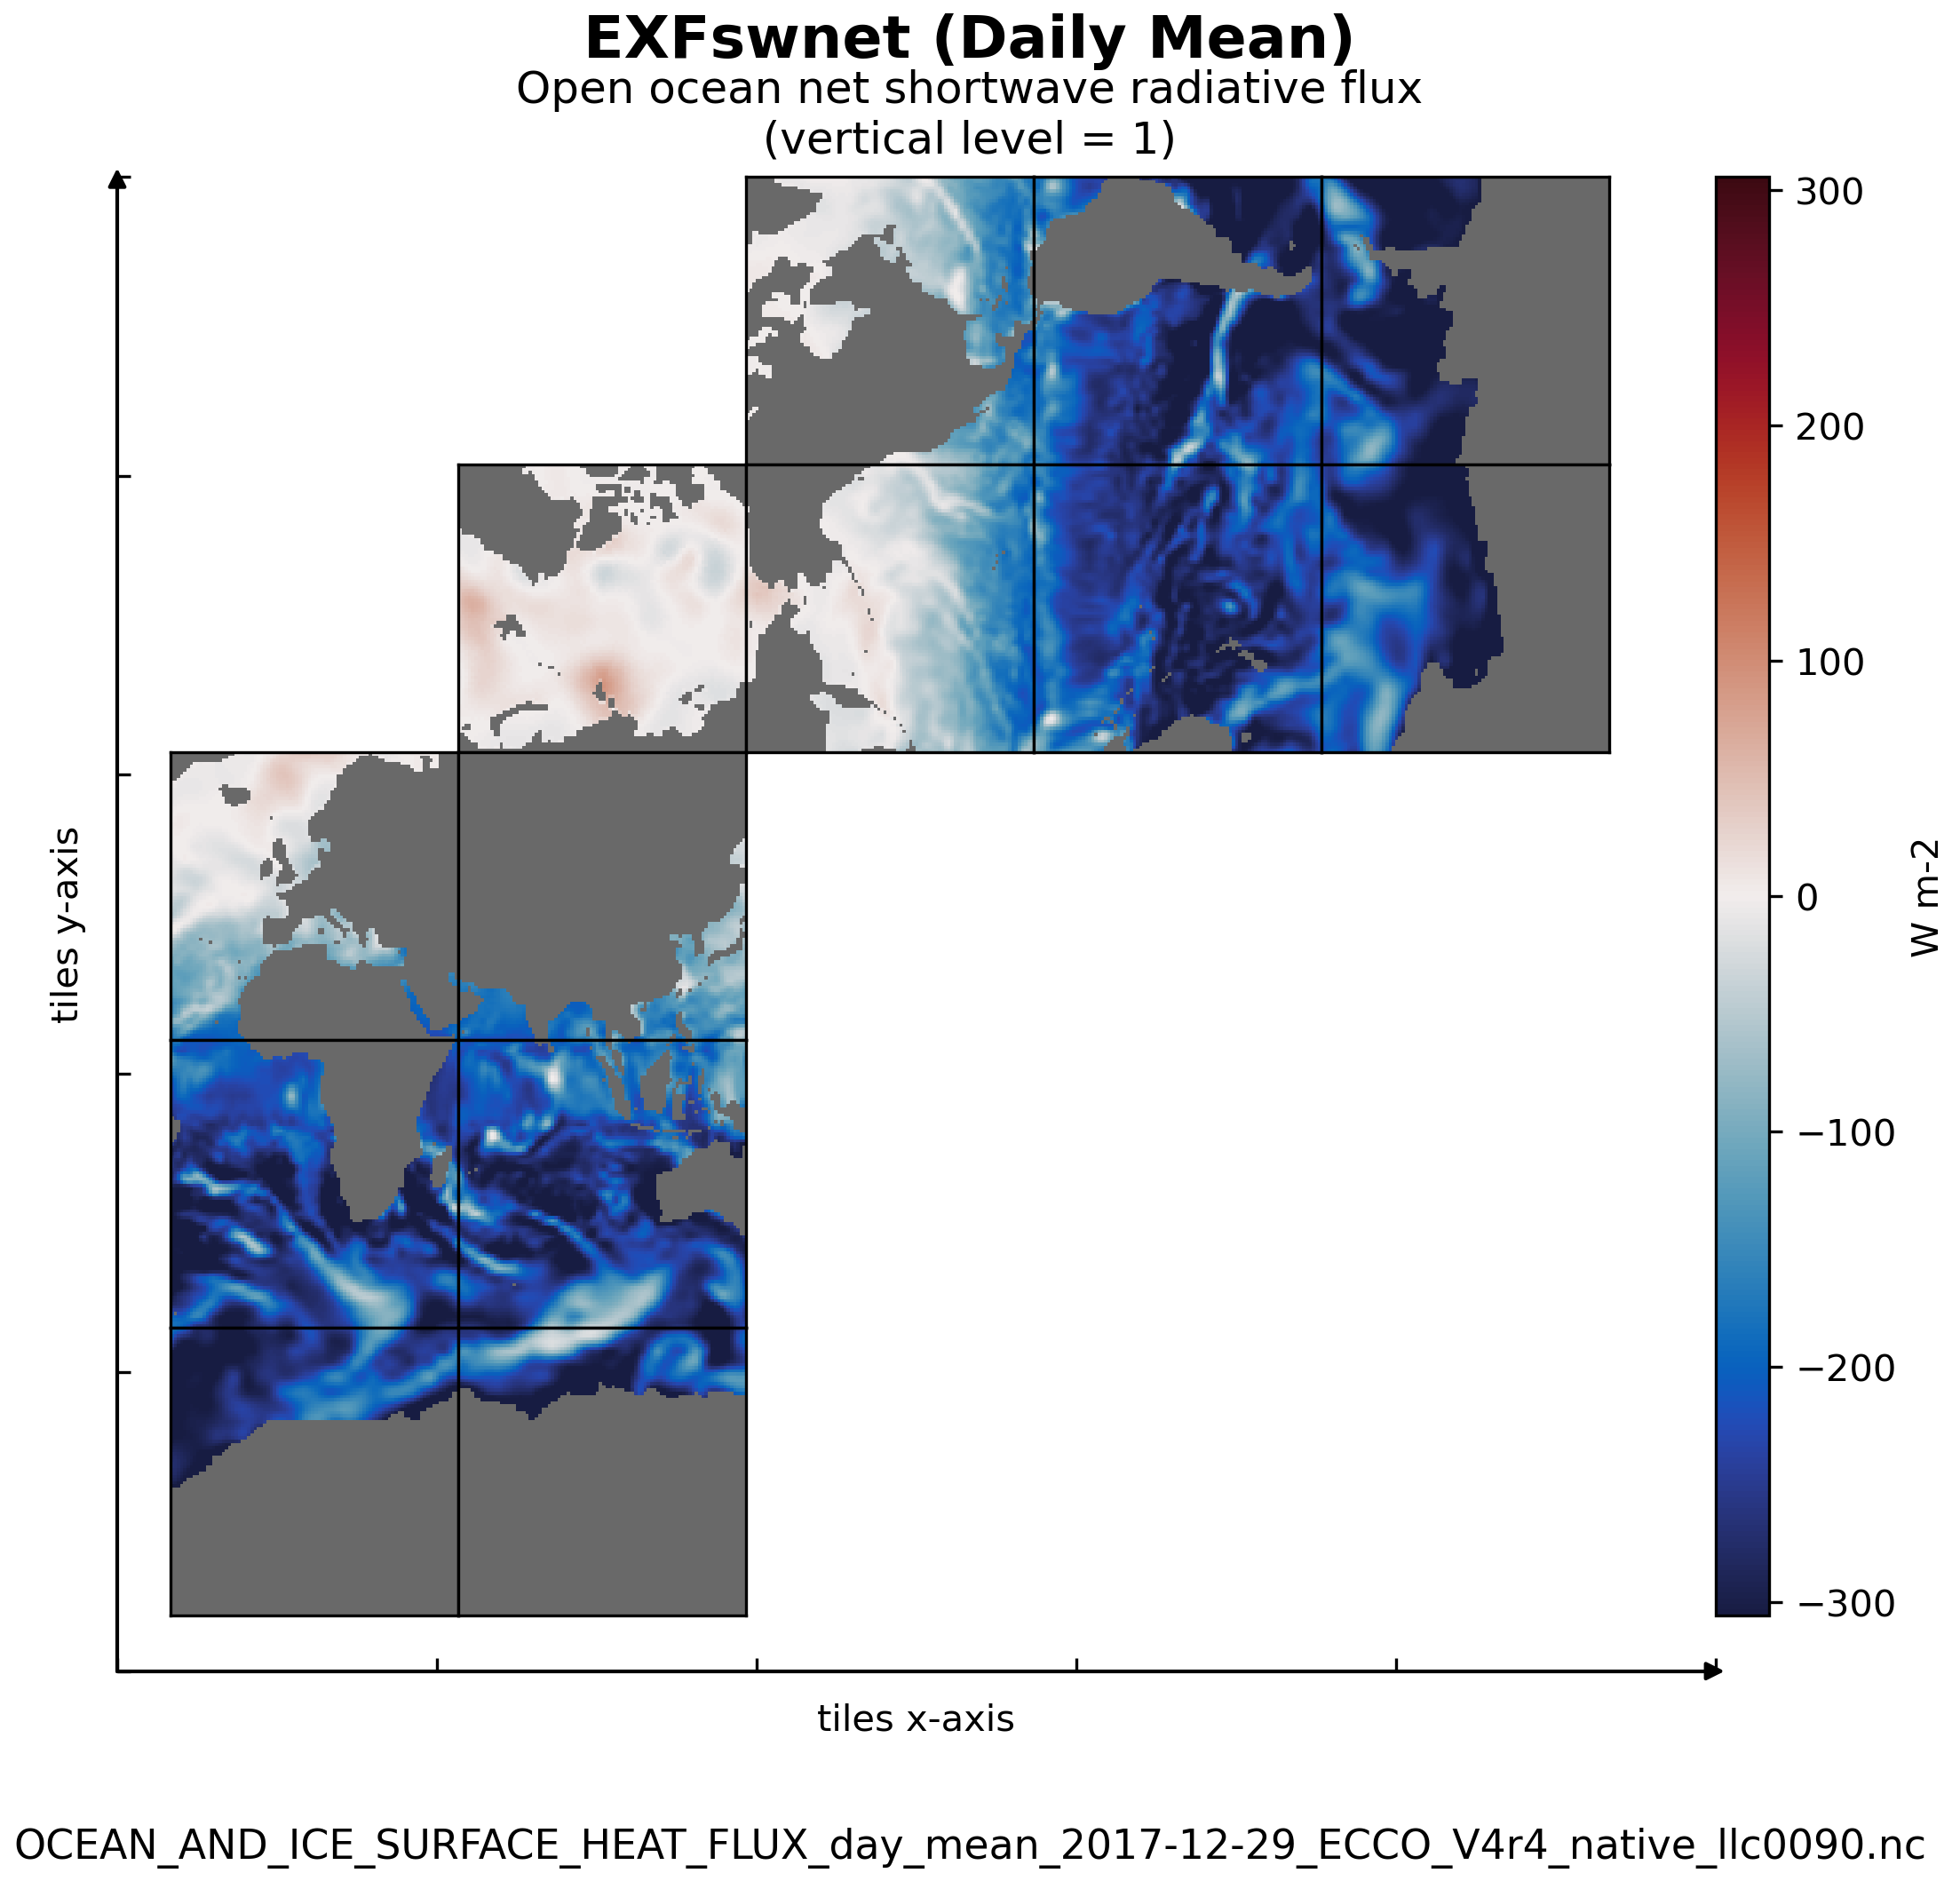
\includegraphics[scale=0.55]{../images/plots/v4r4/native_plots/Ocean_and_Sea-Ice_Surface_Heat_Fluxes/EXFswnet.png}
\caption{Dataset: OCEAN\_AND\_ICE\_SURFACE\_HEAT\_FLUX, Variable: EXFswnet}
\label{tab:table-OCEAN_AND_ICE_SURFACE_HEAT_FLUX_EXFswnet-Plot}
\end{figure}
\newpage
\pagebreak
\subsubsection{Native Variable: SIaaflux}
\begin{longtable}{|m{0.06\textwidth}|m{0.3\textwidth}|m{0.45\textwidth}|m{0.12\textwidth}|}
\caption{Attributes description of the variable 'SIaaflux' from OCEAN\_AND\_ICE\_SURFACE\_HEAT\_FLUX's  dataset.}
\label{tab:table-OCEAN_AND_ICE_SURFACE_HEAT_FLUX_SIaaflux} \\ 
\hline \endhead \hline \endfoot
\rowcolor{lightgray} \textbf{Storage Type} & \textbf{Variable Name} & \textbf{Description} & \textbf{Unit} \\ \hline
float32 & SIaaflux & Conservative ocean and sea-ice advective heat flux adjustment & W m-2 \\ \hline
\multicolumn{4}{|c|}{\cellcolor{lightgray}{\textbf{Description of the variable in Common Data language (CDL)}}} \\ \hline
\multicolumn{4}{|c|}{\fontfamily{lmtt}\selectfont{\makecell{\parbox{.95\textwidth}{\vspace*{0.25cm} \footnotesize{float32 SIaaflux(time, tile, j, i)\\
\hspace*{0.5cm}SIaaflux: \_FillValue = 9.96921e+36\\
\hspace*{0.5cm}SIaaflux: coordinates = XC time YC\\
\hspace*{0.5cm}SIaaflux: coverage\_content\_type = modelResult\\
\hspace*{0.5cm}SIaaflux: direction = >0 decrease potential temperature (THETA)\\
\hspace*{0.5cm}SIaaflux: long\_name = Conservative ocean and sea-ice advective heat flux adjustment\\
\hspace*{0.5cm}SIaaflux: units = W m-2\\
\hspace*{0.5cm}SIaaflux: valid\_max = 50.35451889038086\\
\hspace*{0.5cm}SIaaflux: valid\_min = -16.214622497558594\\
}}}}} \\ \hline
\rowcolor{lightgray} \multicolumn{4}{|c|}{\textbf{Comments}} \\ \hline
\multicolumn{4}{|p{1\textwidth}|}{\footnotesize{{Heat flux associated with the temperature difference between sea surface temperature and sea-ice (assume 0 degree c in the model). note: heat flux needed to melt/freeze sea-ice at 0 degc to sea water at the ocean surface (at sea surface temperature), excluding the latent heat of fusion.}}} \\ \hline
\end{longtable}

\begin{figure}[H]
\centering
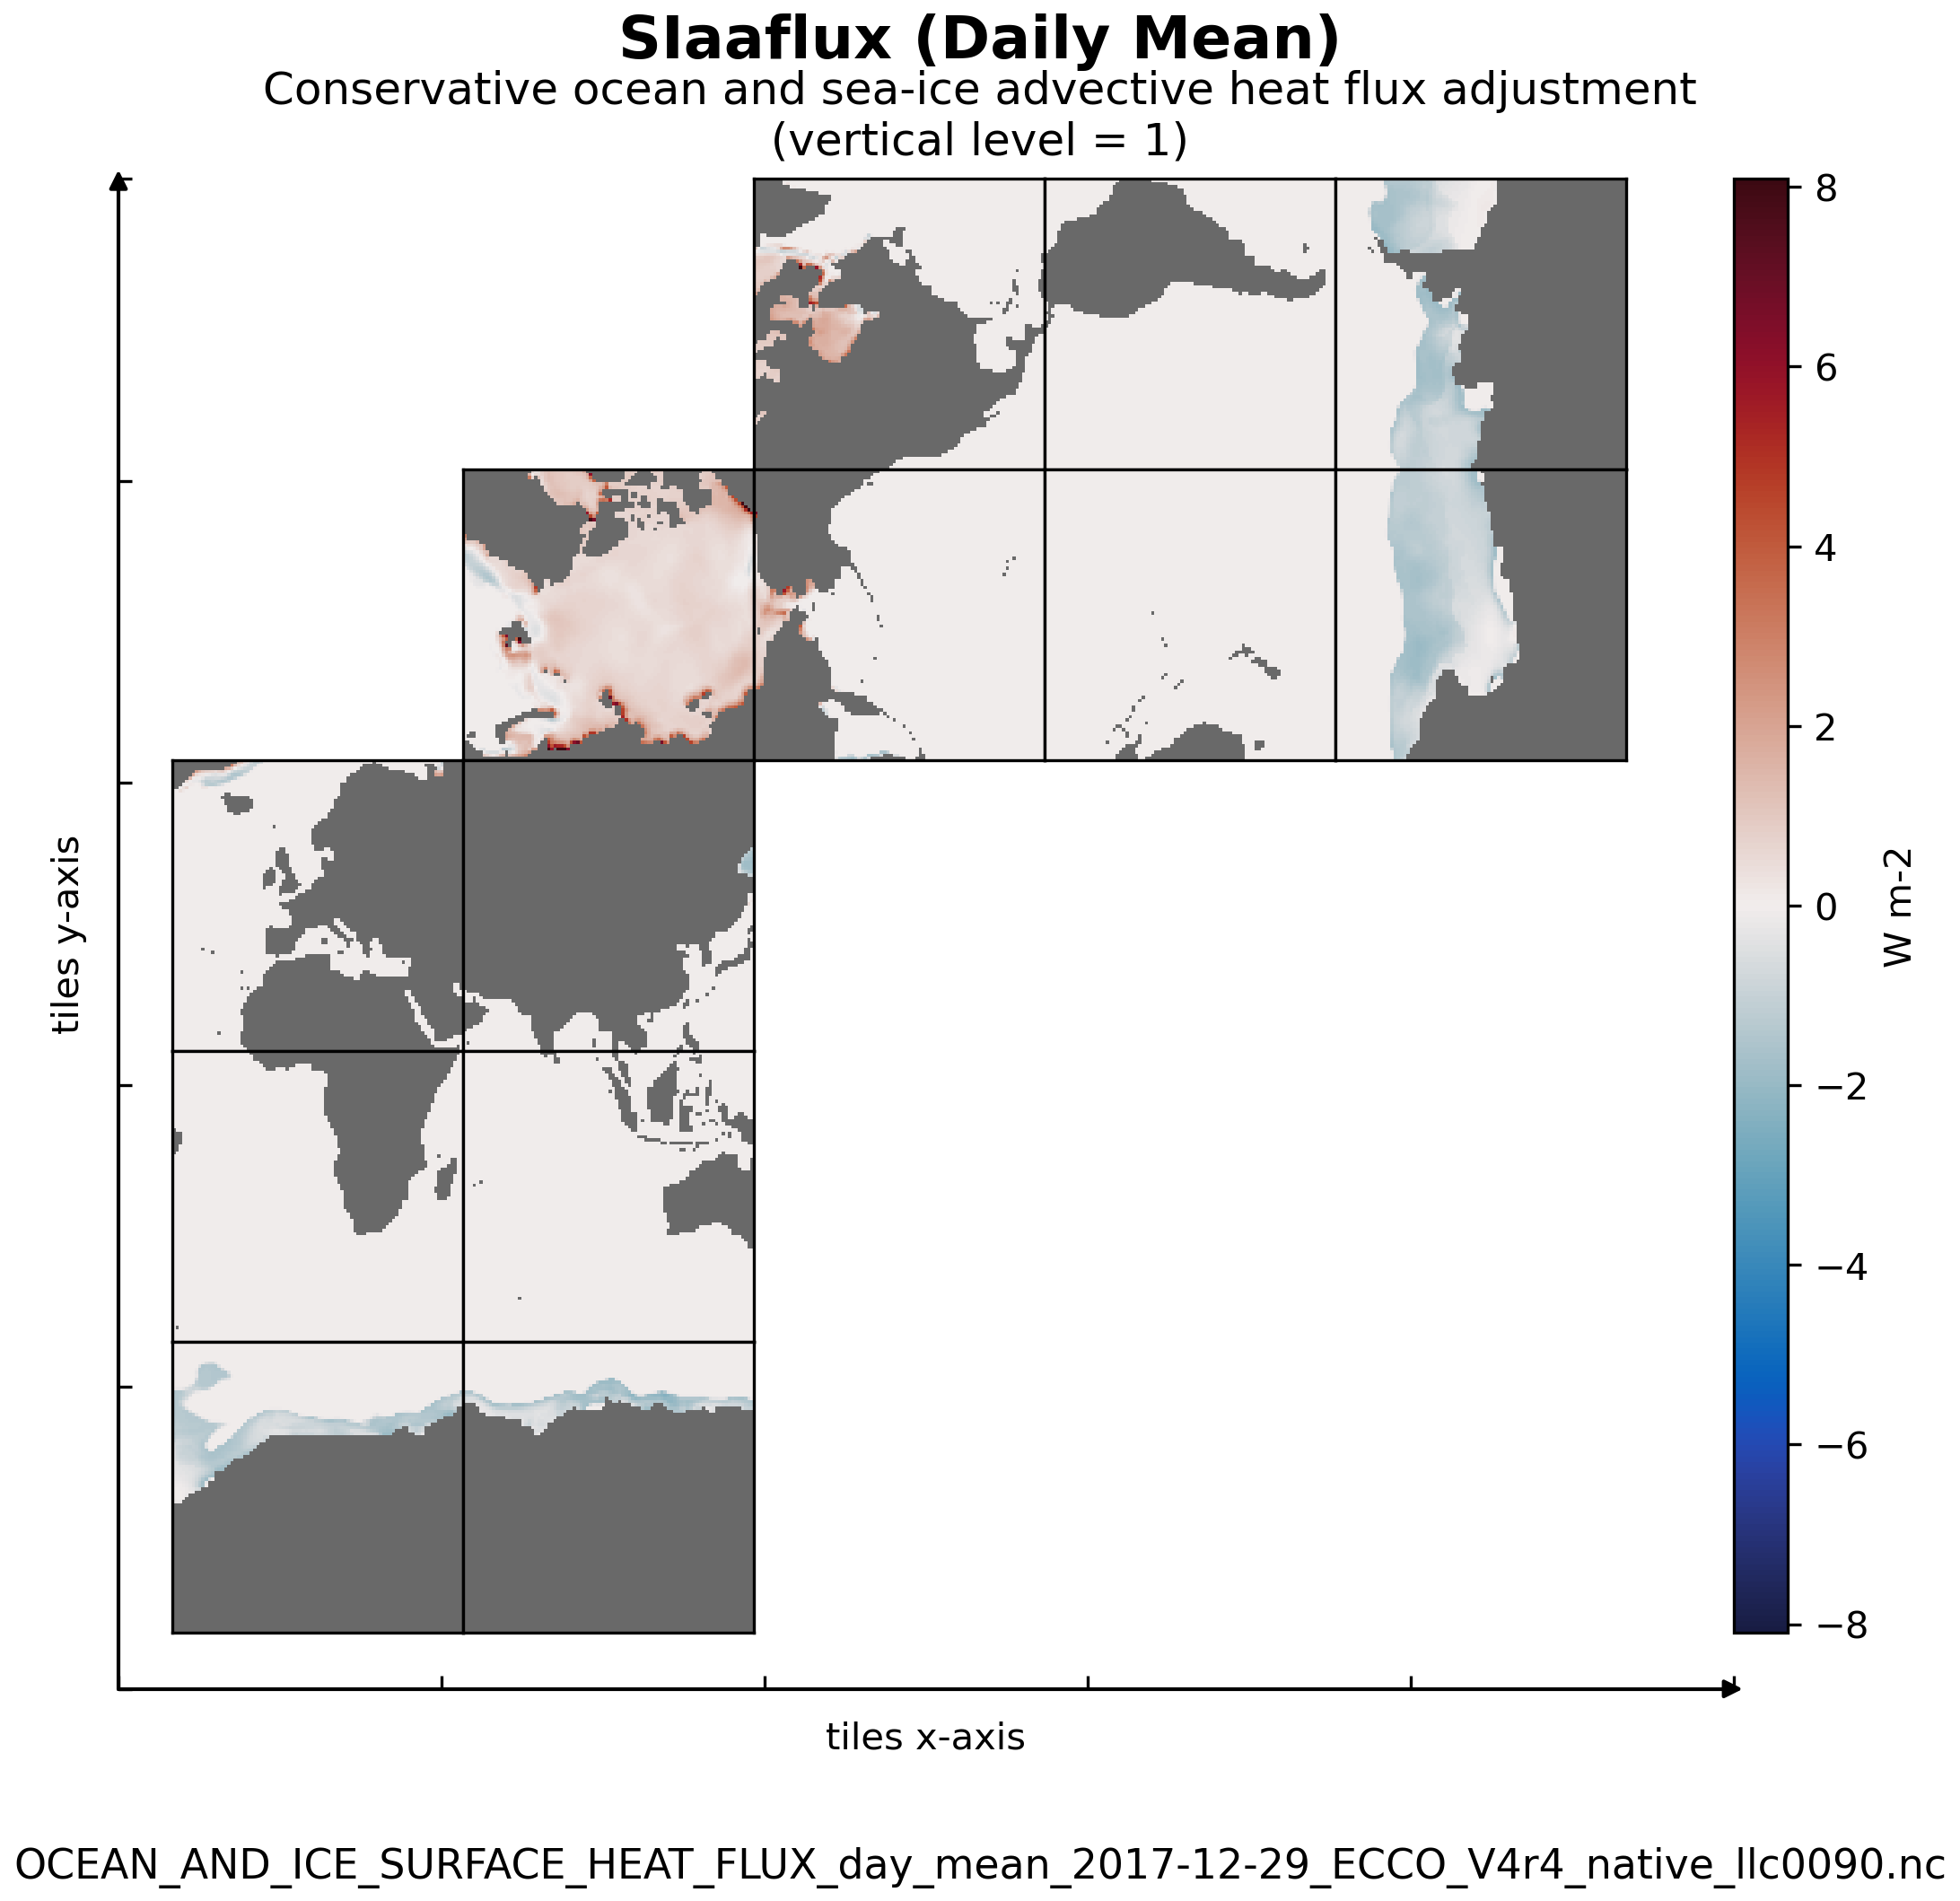
\includegraphics[scale=0.55]{../images/plots/v4r4/native_plots/Ocean_and_Sea-Ice_Surface_Heat_Fluxes/SIaaflux.png}
\caption{Dataset: OCEAN\_AND\_ICE\_SURFACE\_HEAT\_FLUX, Variable: SIaaflux}
\label{tab:table-OCEAN_AND_ICE_SURFACE_HEAT_FLUX_SIaaflux-Plot}
\end{figure}
\newpage
\pagebreak
\subsubsection{Native Variable: SIatmQnt}
\begin{longtable}{|m{0.06\textwidth}|m{0.3\textwidth}|m{0.45\textwidth}|m{0.12\textwidth}|}
\caption{Attributes description of the variable 'SIatmQnt' from OCEAN\_AND\_ICE\_SURFACE\_HEAT\_FLUX's  dataset.}
\label{tab:table-OCEAN_AND_ICE_SURFACE_HEAT_FLUX_SIatmQnt} \\ 
\hline \endhead \hline \endfoot
\rowcolor{lightgray} \textbf{Storage Type} & \textbf{Variable Name} & \textbf{Description} & \textbf{Unit} \\ \hline
float32 & SIatmQnt & Net upward heat flux to the atmosphere & W m-2 \\ \hline
\multicolumn{4}{|c|}{\cellcolor{lightgray}{\textbf{Description of the variable in Common Data language (CDL)}}} \\ \hline
\multicolumn{4}{|c|}{\fontfamily{lmtt}\selectfont{\makecell{\parbox{.95\textwidth}{\vspace*{0.25cm} \footnotesize{float32 SIatmQnt(time, tile, j, i)\\
\hspace*{0.5cm}SIatmQnt: \_FillValue = 9.96921e+36\\
\hspace*{0.5cm}SIatmQnt: coordinates = XC time YC\\
\hspace*{0.5cm}SIatmQnt: coverage\_content\_type = modelResult\\
\hspace*{0.5cm}SIatmQnt: direction = >0 upward, decreases ocean temperature\\
\hspace*{0.5cm}SIatmQnt: long\_name = Net upward heat flux to the atmosphere\\
\hspace*{0.5cm}SIatmQnt: standard\_name = surface upward heat flux in air\\
\hspace*{0.5cm}SIatmQnt: units = W m-2\\
\hspace*{0.5cm}SIatmQnt: valid\_max = 1704.7703857421875\\
\hspace*{0.5cm}SIatmQnt: valid\_min = -756.0607299804688\\
}}}}} \\ \hline
\rowcolor{lightgray} \multicolumn{4}{|c|}{\textbf{Comments}} \\ \hline
\multicolumn{4}{|p{1\textwidth}|}{\footnotesize{{Net upward heat flux to the atmosphere across open water and sea-ice or snow surfaces. note: nonzero siatmqnt may not be associated with a change in ocean potential temperature due to sea-ice growth or melting. to calculate total ocean heat content changes use the variable tflux which also accounts for changing ocean mass (e.g. ocefwflx).}}} \\ \hline
\end{longtable}

\begin{figure}[H]
\centering
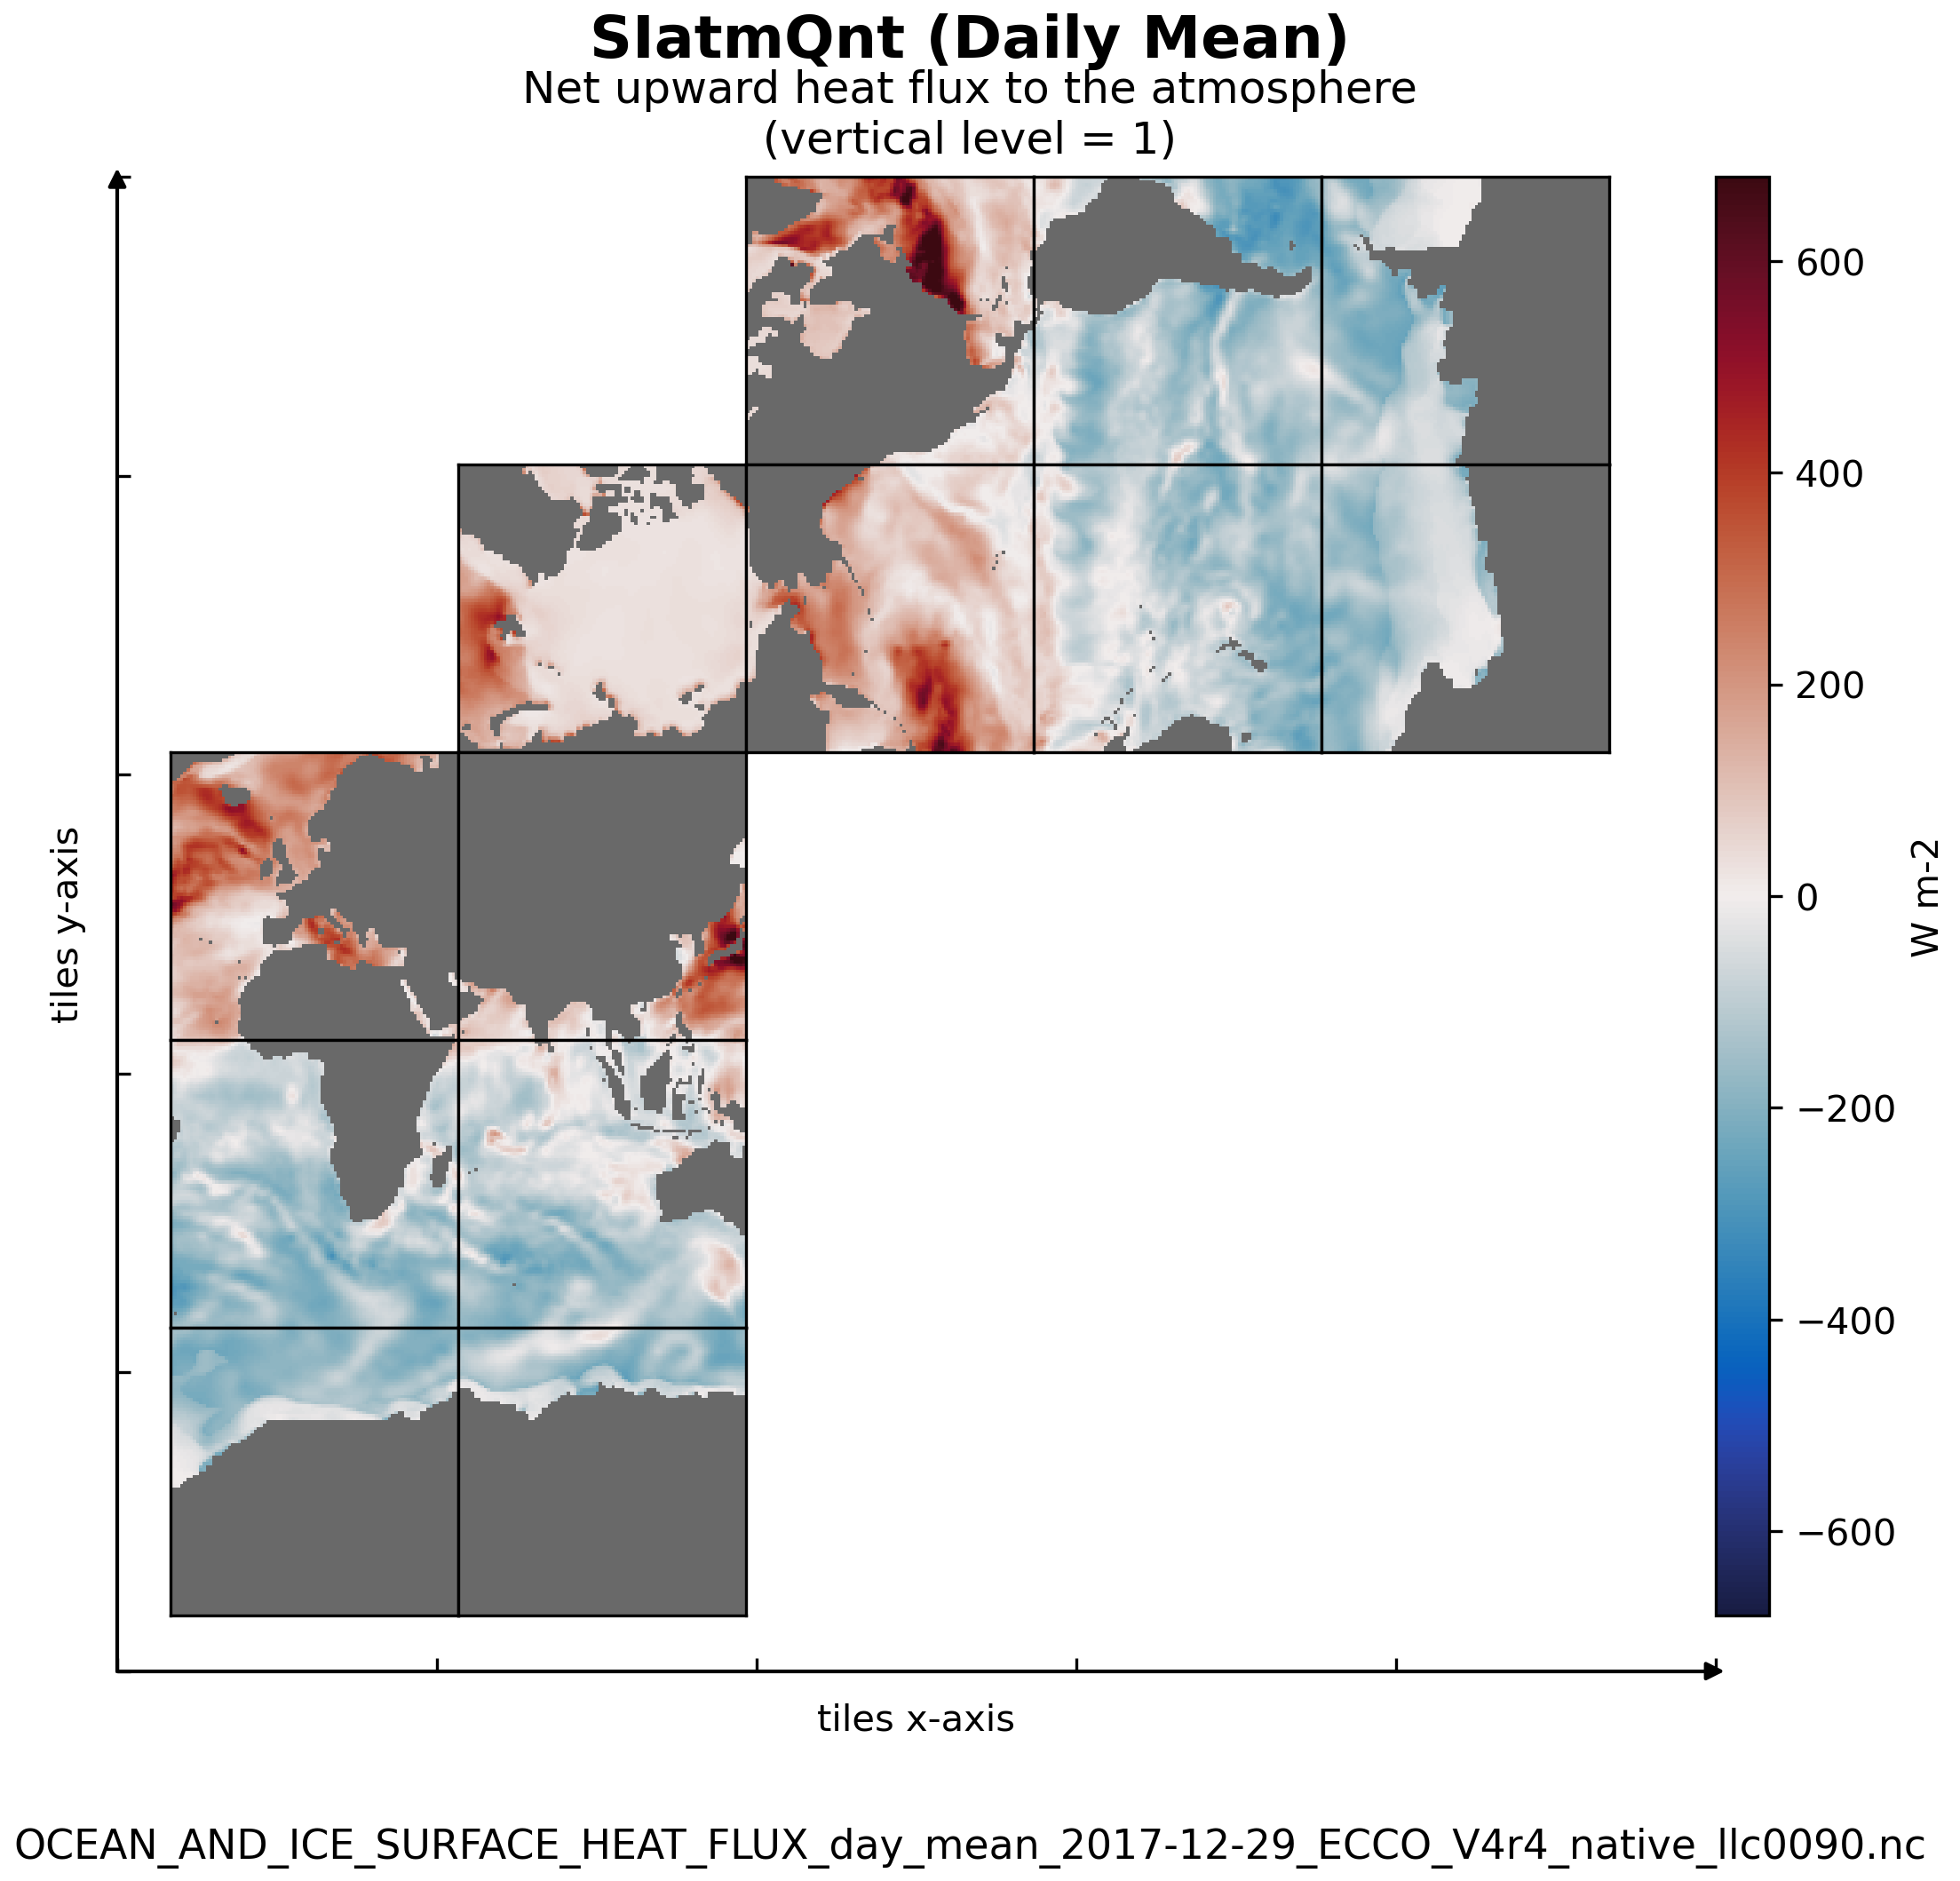
\includegraphics[scale=0.55]{../images/plots/v4r4/native_plots/Ocean_and_Sea-Ice_Surface_Heat_Fluxes/SIatmQnt.png}
\caption{Dataset: OCEAN\_AND\_ICE\_SURFACE\_HEAT\_FLUX, Variable: SIatmQnt}
\label{tab:table-OCEAN_AND_ICE_SURFACE_HEAT_FLUX_SIatmQnt-Plot}
\end{figure}
\newpage
\pagebreak
\subsubsection{Native Variable: TFLUX}
\begin{longtable}{|m{0.06\textwidth}|m{0.3\textwidth}|m{0.45\textwidth}|m{0.12\textwidth}|}
\caption{Attributes description of the variable 'TFLUX' from OCEAN\_AND\_ICE\_SURFACE\_HEAT\_FLUX's  dataset.}
\label{tab:table-OCEAN_AND_ICE_SURFACE_HEAT_FLUX_TFLUX} \\ 
\hline \endhead \hline \endfoot
\rowcolor{lightgray} \textbf{Storage Type} & \textbf{Variable Name} & \textbf{Description} & \textbf{Unit} \\ \hline
float32 & TFLUX & Rate of change of ocean heat content per m2 accounting for mass fluxes. & W m-2 \\ \hline
\multicolumn{4}{|c|}{\cellcolor{lightgray}{\textbf{Description of the variable in Common Data language (CDL)}}} \\ \hline
\multicolumn{4}{|c|}{\fontfamily{lmtt}\selectfont{\makecell{\parbox{.95\textwidth}{\vspace*{0.25cm} \footnotesize{float32 TFLUX(time, tile, j, i)\\
\hspace*{0.5cm}TFLUX: \_FillValue = 9.96921e+36\\
\hspace*{0.5cm}TFLUX: coordinates = XC time YC\\
\hspace*{0.5cm}TFLUX: coverage\_content\_type = modelResult\\
\hspace*{0.5cm}TFLUX: direction = >0 increases potential temperature (THETA)\\
\hspace*{0.5cm}TFLUX: long\_name = Rate of change of ocean heat content per m2 accounting for mass fluxes.\\
\hspace*{0.5cm}TFLUX: units = W m-2\\
\hspace*{0.5cm}TFLUX: valid\_max = 870.3130493164062\\
\hspace*{0.5cm}TFLUX: valid\_min = -1713.51220703125\\
}}}}} \\ \hline
\rowcolor{lightgray} \multicolumn{4}{|c|}{\textbf{Comments}} \\ \hline
\multicolumn{4}{|p{1\textwidth}|}{\footnotesize{{The rate of change of ocean heat content due to heat fluxes across the liquid surface and the addition or removal of mass. . note: the global area integral of tflux and geothermal flux (geothermalflux.bin) matches the time-derivative of ocean heat content (j/s). unlike oceqnet, tflux includes the contribution to the ocean heat content from changing ocean mass (e.g. from ocefwflx).}}} \\ \hline
\end{longtable}

\begin{figure}[H]
\centering
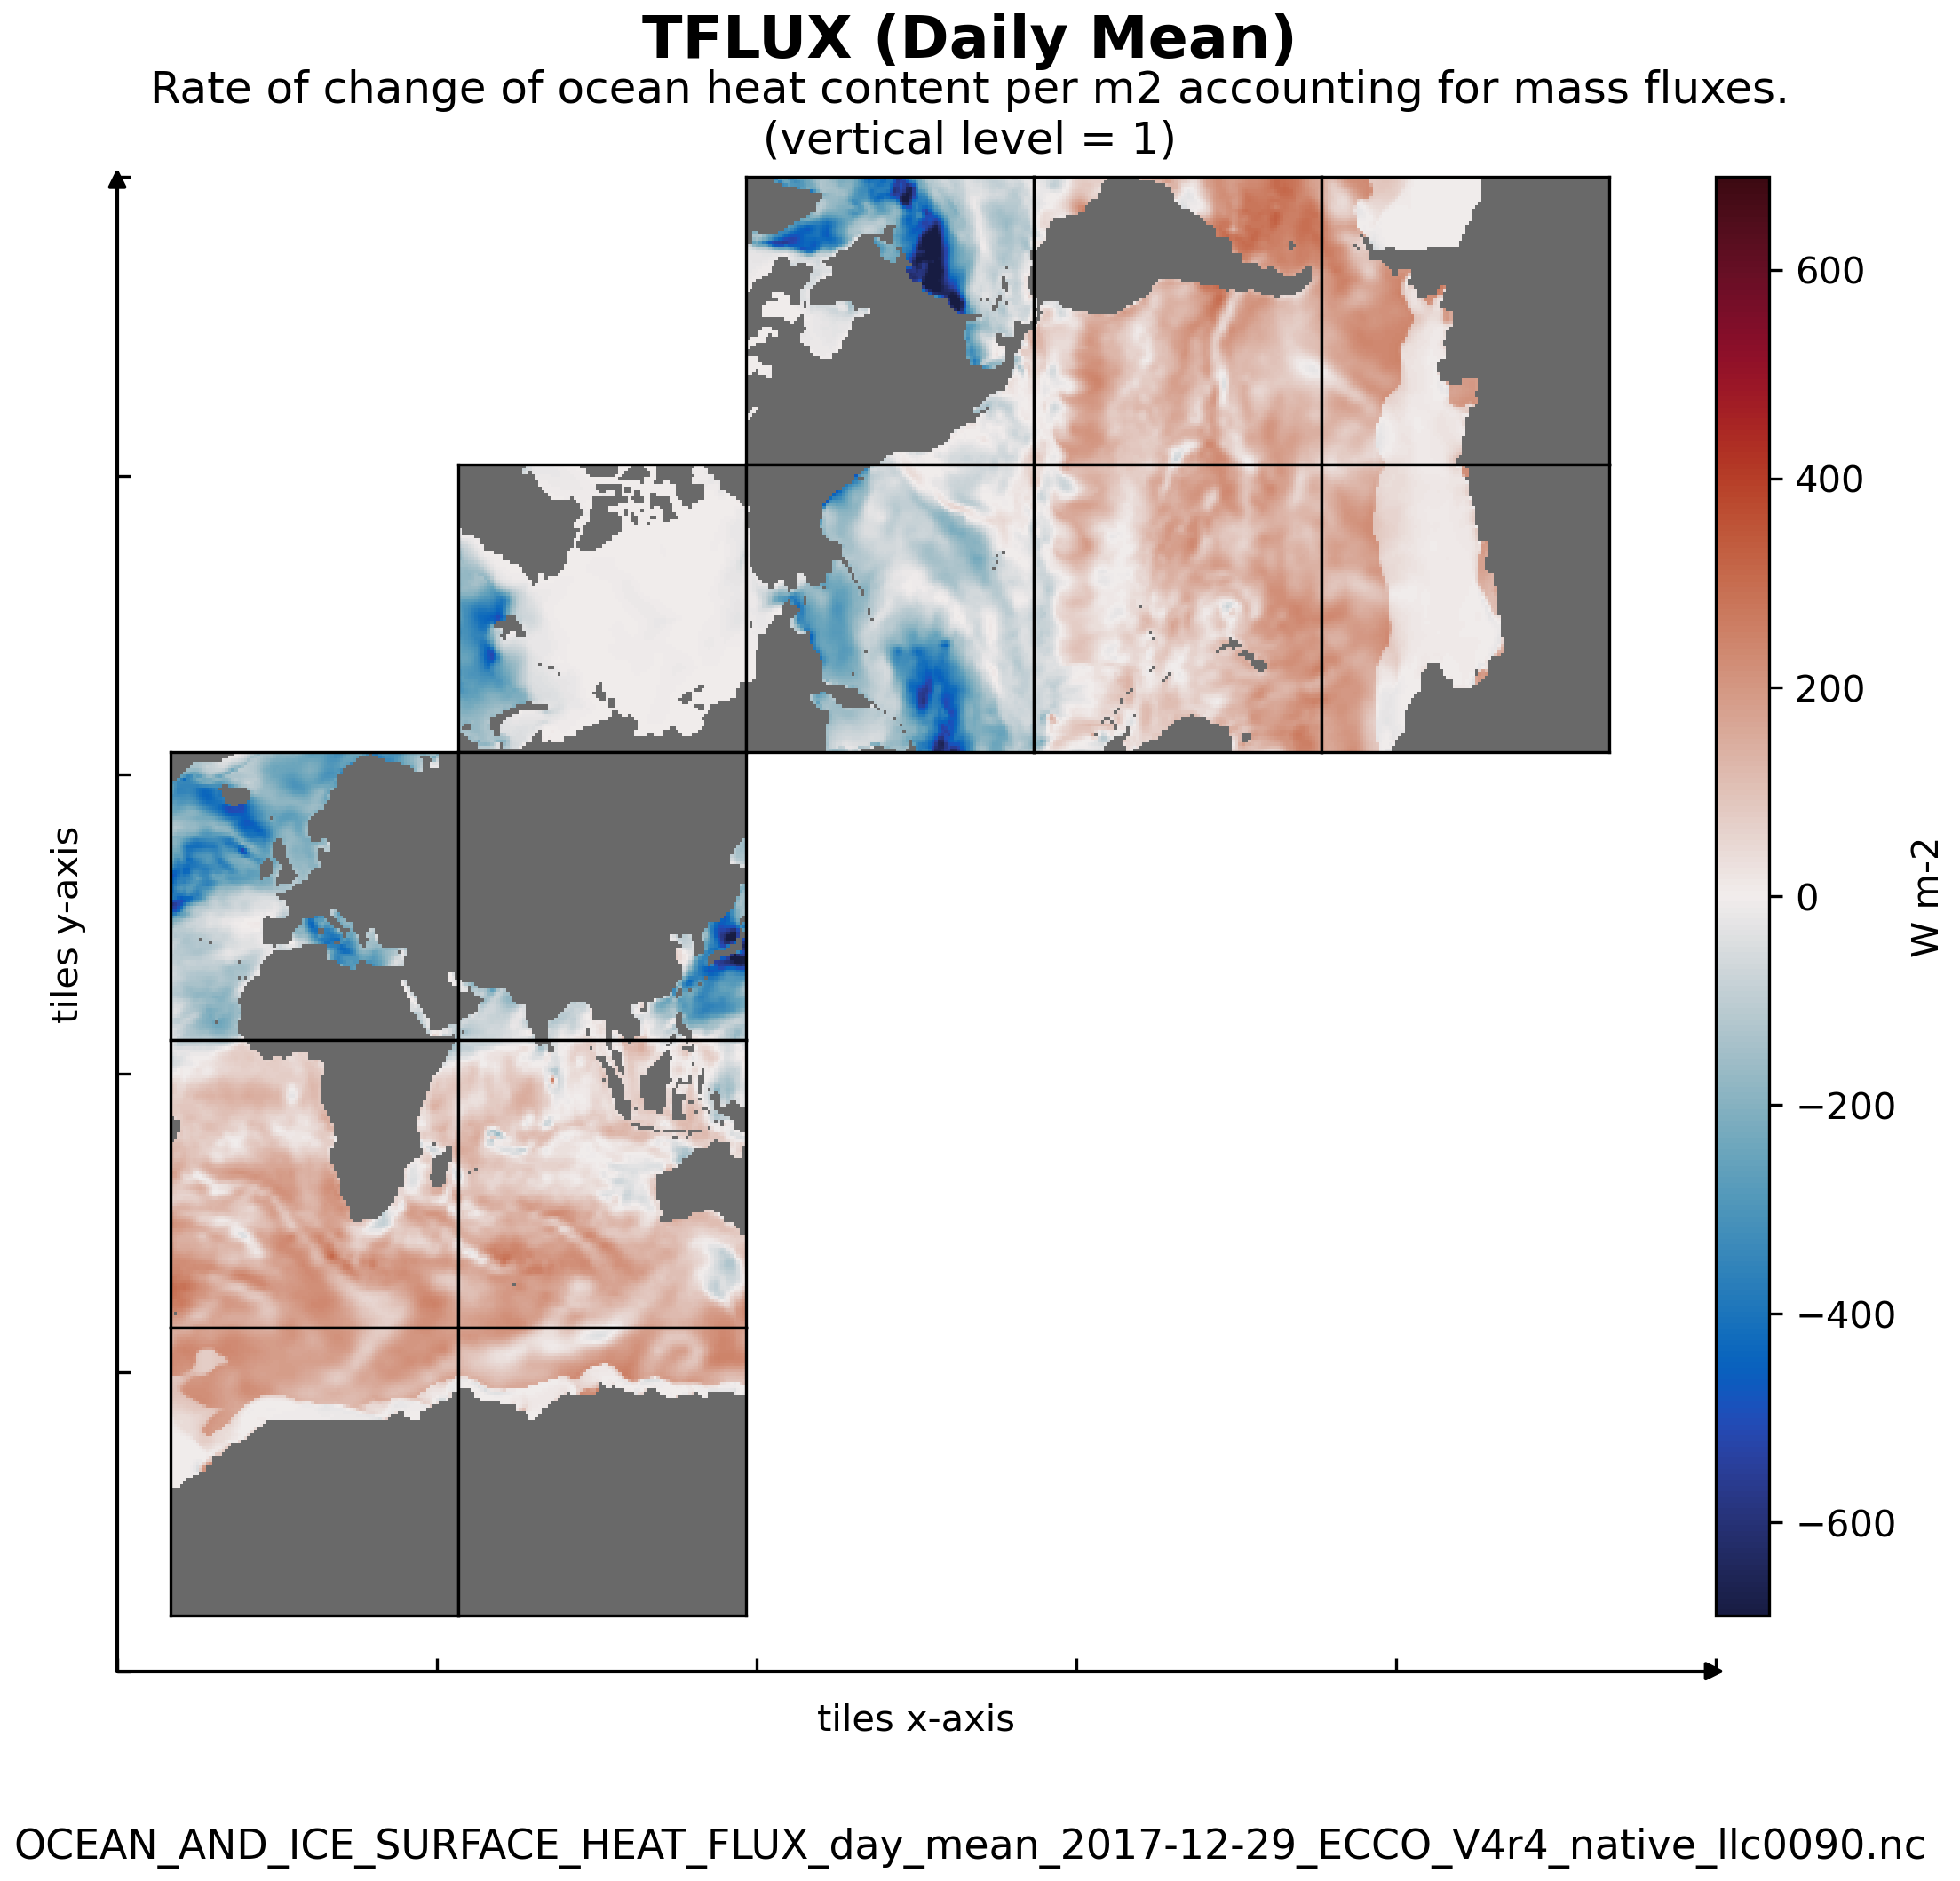
\includegraphics[scale=0.55]{../images/plots/v4r4/native_plots/Ocean_and_Sea-Ice_Surface_Heat_Fluxes/TFLUX.png}
\caption{Dataset: OCEAN\_AND\_ICE\_SURFACE\_HEAT\_FLUX, Variable: TFLUX}
\label{tab:table-OCEAN_AND_ICE_SURFACE_HEAT_FLUX_TFLUX-Plot}
\end{figure}
\newpage
\pagebreak
\subsubsection{Native Variable: oceQnet}
\begin{longtable}{|m{0.06\textwidth}|m{0.3\textwidth}|m{0.45\textwidth}|m{0.12\textwidth}|}
\caption{Attributes description of the variable 'oceQnet' from OCEAN\_AND\_ICE\_SURFACE\_HEAT\_FLUX's  dataset.}
\label{tab:table-OCEAN_AND_ICE_SURFACE_HEAT_FLUX_oceQnet} \\ 
\hline \endhead \hline \endfoot
\rowcolor{lightgray} \textbf{Storage Type} & \textbf{Variable Name} & \textbf{Description} & \textbf{Unit} \\ \hline
float32 & oceQnet & Net heat flux into the ocean surface & W m-2 \\ \hline
\multicolumn{4}{|c|}{\cellcolor{lightgray}{\textbf{Description of the variable in Common Data language (CDL)}}} \\ \hline
\multicolumn{4}{|c|}{\fontfamily{lmtt}\selectfont{\makecell{\parbox{.95\textwidth}{\vspace*{0.25cm} \footnotesize{float32 oceQnet(time, tile, j, i)\\
\hspace*{0.5cm}oceQnet: \_FillValue = 9.96921e+36\\
\hspace*{0.5cm}oceQnet: coordinates = XC time YC\\
\hspace*{0.5cm}oceQnet: coverage\_content\_type = modelResult\\
\hspace*{0.5cm}oceQnet: direction = >0 increases potential temperature (THETA)\\
\hspace*{0.5cm}oceQnet: long\_name = Net heat flux into the ocean surface\\
\hspace*{0.5cm}oceQnet: standard\_name = surface downward heat flux in sea water\\
\hspace*{0.5cm}oceQnet: units = W m-2\\
\hspace*{0.5cm}oceQnet: valid\_max = 675.3716430664062\\
\hspace*{0.5cm}oceQnet: valid\_min = -1708.8460693359375\\
}}}}} \\ \hline
\rowcolor{lightgray} \multicolumn{4}{|c|}{\textbf{Comments}} \\ \hline
\multicolumn{4}{|p{1\textwidth}|}{\footnotesize{{Net heat flux into the ocean surface from all processes: air-sea turbulent and radiative fluxes and turbulent and conductive fluxes between the ocean and sea-ice and snow. note: oceqnet does not include the change in ocean heat content due to changing ocean ocean mass (ocefwflx). mass fluxes from evaporation, precipitation, and runoff (exfempmr) happen at the same temperature as the ocean surface temperature. consequently, empmr does not change ocean surface temperature. conversely, mass fluxes due to sea-ice thickening/thinning and snow melt in the model are assumed to happen at a fixed 0c. consequently, mass fluxes due to phase changes between seawater and sea-ice and snow induce a heat flux when the ocean surface temperaure is not 0c. the variable tflux does include the change in ocean heat content due to changing ocean mass.}}} \\ \hline
\end{longtable}

\begin{figure}[H]
\centering
\includegraphics[scale=0.55]{../images/plots/v4r4/native_plots/Ocean_and_Sea-Ice_Surface_Heat_Fluxes/oceQnet.png}
\caption{Dataset: OCEAN\_AND\_ICE\_SURFACE\_HEAT\_FLUX, Variable: oceQnet}
\label{tab:table-OCEAN_AND_ICE_SURFACE_HEAT_FLUX_oceQnet-Plot}
\end{figure}
\newpage
\pagebreak
\subsubsection{Native Variable: oceQsw}
\begin{longtable}{|m{0.06\textwidth}|m{0.3\textwidth}|m{0.45\textwidth}|m{0.12\textwidth}|}
\caption{Attributes description of the variable 'oceQsw' from OCEAN\_AND\_ICE\_SURFACE\_HEAT\_FLUX's  dataset.}
\label{tab:table-OCEAN_AND_ICE_SURFACE_HEAT_FLUX_oceQsw} \\ 
\hline \endhead \hline \endfoot
\rowcolor{lightgray} \textbf{Storage Type} & \textbf{Variable Name} & \textbf{Description} & \textbf{Unit} \\ \hline
float32 & oceQsw & Net shortwave radiative flux across the ocean surface & W m-2 \\ \hline
\multicolumn{4}{|c|}{\cellcolor{lightgray}{\textbf{Description of the variable in Common Data language (CDL)}}} \\ \hline
\multicolumn{4}{|c|}{\fontfamily{lmtt}\selectfont{\makecell{\parbox{.95\textwidth}{\vspace*{0.25cm} \footnotesize{float32 oceQsw(time, tile, j, i)\\
\hspace*{0.5cm}oceQsw: \_FillValue = 9.96921e+36\\
\hspace*{0.5cm}oceQsw: coordinates = XC time YC\\
\hspace*{0.5cm}oceQsw: coverage\_content\_type = modelResult\\
\hspace*{0.5cm}oceQsw: direction = >0 increases potential temperature (THETA)\\
\hspace*{0.5cm}oceQsw: long\_name = Net shortwave radiative flux across the ocean surface\\
\hspace*{0.5cm}oceQsw: units = W m-2\\
\hspace*{0.5cm}oceQsw: valid\_max = 655.6171264648438\\
\hspace*{0.5cm}oceQsw: valid\_min = -134.39808654785156\\
}}}}} \\ \hline
\rowcolor{lightgray} \multicolumn{4}{|c|}{\textbf{Comments}} \\ \hline
\multicolumn{4}{|p{1\textwidth}|}{\footnotesize{{Net shortwave radiative flux across the ocean surface. note: shortwave radiation penetrates below the surface grid cell.}}} \\ \hline
\end{longtable}

\begin{figure}[H]
\centering
\includegraphics[scale=0.55]{../images/plots/v4r4/native_plots/Ocean_and_Sea-Ice_Surface_Heat_Fluxes/oceQsw.png}
\caption{Dataset: OCEAN\_AND\_ICE\_SURFACE\_HEAT\_FLUX, Variable: oceQsw}
\label{tab:table-OCEAN_AND_ICE_SURFACE_HEAT_FLUX_oceQsw-Plot}
\end{figure}
\newpage
\subsection{Native dataset of OCEAN\_AND\_ICE\_SURFACE\_STRESS}
\newp
\subsubsection{Overview}
This dataset provides 2D fields of ocean and sea-ice surface stress on the lat-lon-cap 90 (llc90) native model grid from the ECCO Version 4 Release 4 (V4r4) ocean and sea-ice state estimate. The dataset is provided on daily-average and monthly-average time resolution. 
\begin{longtable}{|m{0.15\textwidth}|m{0.64\textwidth}|m{0.12\textwidth}|}
\caption{Coordinates and Variables in the dataset OCEAN\_AND\_ICE\_SURFACE\_STRESS}
\label{tab:table-OCEAN_AND_ICE_SURFACE_STRESS-fields} \\ 
\hline \endhead \hline \endfoot
\rowcolor{lightgray} \multicolumn{1}{|c|}{\textbf{Coordinates}} & \multicolumn{1}{|c|}{\textbf{Description of data coordinates}} &  \multicolumn{1}{|c|}{\textbf{Unit}}\\ \hline
i &Grid index in x for variables at tracer and 'v' locations &--none--  \\ \hline
i\_g &Grid index in x for variables at 'u' and 'g' locations &--none--  \\ \hline
j &Grid index in y for variables at tracer and 'u' locations &--none--  \\ \hline
j\_g &Grid index in y for variables at 'v' and 'g' locations &--none--  \\ \hline
tile &Lat-lon-cap tile index &--none--  \\ \hline
time &Center time of averaging period &--none--  \\ \hline
XC &Longitude of tracer grid cell center &degrees\_east  \\ \hline
YC &Latitude of tracer grid cell center &degrees\_north  \\ \hline
XG &Longitude of 'southwest' corner of tracer grid cell &degrees\_east  \\ \hline
YG &Latitude of 'southwest' corner of tracer grid cell &degrees\_north  \\ \hline
time\_bnds &Time bounds of averaging period &--none--  \\ \hline
XC\_bnds &Longitudes of tracer grid cell corners &--none--  \\ \hline
YC\_bnds &Latitudes of tracer grid cell corners &--none--  \\ \hline
\rowcolor{lightgray} \multicolumn{1}{|c|}{\textbf{Variables}} & \multicolumn{1}{|c|}{\textbf{Description of data variables}} &  \multicolumn{1}{|c|}{\textbf{Unit}}\\ \hline
EXFtaux &Wind stress in the model +x direction &N m-2  \\ \hline
EXFtauy &Wind stress in the model +y direction &N m-2  \\ \hline
oceTAUX &Ocean surface stress in the model +x direction &N m-2  \\ \hline
oceTAUY &Ocean surface stress in the model +y direction &N m-2  \\ \hline
\end{longtable}

\newp
\pagebreak
\subsubsection{Native Variable: EXFtaux}
\begin{longtable}{|m{0.06\textwidth}|m{0.3\textwidth}|m{0.45\textwidth}|m{0.12\textwidth}|}
\caption{Attributes description of the variable 'EXFtaux' from OCEAN\_AND\_ICE\_SURFACE\_STRESS's  dataset.}
\label{tab:table-OCEAN_AND_ICE_SURFACE_STRESS_EXFtaux} \\ 
\hline \endhead \hline \endfoot
\rowcolor{lightgray} \textbf{Storage Type} & \textbf{Variable Name} & \textbf{Description} & \textbf{Unit} \\ \hline
float32 & EXFtaux & Wind stress in the model +x direction & N m-2 \\ \hline
\multicolumn{4}{|c|}{\cellcolor{lightgray}{\textbf{Description of the variable in Common Data language (CDL)}}} \\ \hline
\multicolumn{4}{|c|}{\fontfamily{lmtt}\selectfont{\makecell{\parbox{.95\textwidth}{\vspace*{0.25cm} \footnotesize{float32 EXFtaux(time, tile, j, i)\\
\hspace*{0.5cm}EXFtaux: \_FillValue = 9.96921e+36\\
\hspace*{0.5cm}EXFtaux: coordinates = time YC XC\\
\hspace*{0.5cm}EXFtaux: coverage\_content\_type = modelResult\\
\hspace*{0.5cm}EXFtaux: direction =  >0 increases horizontal velocity in the +x direction (UVEL)\\
\hspace*{0.5cm}EXFtaux: long\_name = Wind stress in the model +x direction\\
\hspace*{0.5cm}EXFtaux: standard\_name = surface downward x stress\\
\hspace*{0.5cm}EXFtaux: units = N m-2\\
\hspace*{0.5cm}EXFtaux: valid\_max = 3.7184090614318848\\
\hspace*{0.5cm}EXFtaux: valid\_min = -7.474303722381592\\
}}}}} \\ \hline
\rowcolor{lightgray} \multicolumn{4}{|c|}{\textbf{Comments}} \\ \hline
\multicolumn{4}{|p{1\textwidth}|}{\footnotesize{{Wind stress in the +x direction at the tracer cell on the native model grid. note: exftaux is the stress applied to the ice-free ocean surface and sea-ice covered surface. when sea-ice is present, the total stress applied to the ocean surface in the +x direction is not exftaux, but a combination of exftaux wind stress in the open water fraction and a stress from sea-ice in the ice-covered fraction (see ocetaux). exftaux is the sum of era-interim stress and the control adjustment from ocean state estimation.}}} \\ \hline
\end{longtable}

\begin{figure}[H]
\centering
\includegraphics[scale=0.55]{../images/plots/v4r4/native_plots/Ocean_and_Sea-Ice_Surface_Stress/EXFtaux.png}
\caption{Dataset: OCEAN\_AND\_ICE\_SURFACE\_STRESS, Variable: EXFtaux}
\label{tab:table-OCEAN_AND_ICE_SURFACE_STRESS_EXFtaux-Plot}
\end{figure}
\newpage
\pagebreak
\subsubsection{Native Variable: EXFtauy}
\begin{longtable}{|m{0.06\textwidth}|m{0.3\textwidth}|m{0.45\textwidth}|m{0.12\textwidth}|}
\caption{Attributes description of the variable 'EXFtauy' from OCEAN\_AND\_ICE\_SURFACE\_STRESS's  dataset.}
\label{tab:table-OCEAN_AND_ICE_SURFACE_STRESS_EXFtauy} \\ 
\hline \endhead \hline \endfoot
\rowcolor{lightgray} \textbf{Storage Type} & \textbf{Variable Name} & \textbf{Description} & \textbf{Unit} \\ \hline
float32 & EXFtauy & Wind stress in the model +y direction & N m-2 \\ \hline
\multicolumn{4}{|c|}{\cellcolor{lightgray}{\textbf{Description of the variable in Common Data language (CDL)}}} \\ \hline
\multicolumn{4}{|c|}{\fontfamily{lmtt}\selectfont{\makecell{\parbox{.95\textwidth}{\vspace*{0.25cm} \footnotesize{float32 EXFtauy(time, tile, j, i)\\
\hspace*{0.5cm}EXFtauy: \_FillValue = 9.96921e+36\\
\hspace*{0.5cm}EXFtauy: coordinates = time YC XC\\
\hspace*{0.5cm}EXFtauy: coverage\_content\_type = modelResult\\
\hspace*{0.5cm}EXFtauy: direction =  >0 increases horizontal velocity in the +y direction (VVEL)\\
\hspace*{0.5cm}EXFtauy: long\_name = Wind stress in the model +y direction\\
\hspace*{0.5cm}EXFtauy: standard\_name = surface downward y stress\\
\hspace*{0.5cm}EXFtauy: units = N m-2\\
\hspace*{0.5cm}EXFtauy: valid\_max = 3.7044837474823\\
\hspace*{0.5cm}EXFtauy: valid\_min = -3.71972918510437\\
}}}}} \\ \hline
\rowcolor{lightgray} \multicolumn{4}{|c|}{\textbf{Comments}} \\ \hline
\multicolumn{4}{|p{1\textwidth}|}{\footnotesize{{Wind stress in the +y direction at the tracer cell on the native model grid. note: exftauy is the stress applied to the ice-free ocean surface and sea-ice covered surface. when sea-ice is present, the total stress applied to the ocean surface in the +y direction is not exftauy, but a combination of exftauy wind stress in the open water fraction and a stress from sea-ice in the ice-covered fraction (see ocetauy). exftaux is the sum of era-interim stress and the control adjustment from ocean state estimation.}}} \\ \hline
\end{longtable}

\begin{figure}[H]
\centering
\includegraphics[scale=0.55]{../images/plots/v4r4/native_plots/Ocean_and_Sea-Ice_Surface_Stress/EXFtauy.png}
\caption{Dataset: OCEAN\_AND\_ICE\_SURFACE\_STRESS, Variable: EXFtauy}
\label{tab:table-OCEAN_AND_ICE_SURFACE_STRESS_EXFtauy-Plot}
\end{figure}
\newpage
\pagebreak
\subsubsection{Native Variable: oceTAUX}
\begin{longtable}{|m{0.06\textwidth}|m{0.3\textwidth}|m{0.45\textwidth}|m{0.12\textwidth}|}
\caption{Attributes description of the variable 'oceTAUX' from OCEAN\_AND\_ICE\_SURFACE\_STRESS's  dataset.}
\label{tab:table-OCEAN_AND_ICE_SURFACE_STRESS_oceTAUX} \\ 
\hline \endhead \hline \endfoot
\rowcolor{lightgray} \textbf{Storage Type} & \textbf{Variable Name} & \textbf{Description} & \textbf{Unit} \\ \hline
float32 & oceTAUX & Ocean surface stress in the model +x direction & N m-2 \\ \hline
\multicolumn{4}{|c|}{\cellcolor{lightgray}{\textbf{Description of the variable in Common Data language (CDL)}}} \\ \hline
\multicolumn{4}{|c|}{\fontfamily{lmtt}\selectfont{\makecell{\parbox{.95\textwidth}{\vspace*{0.25cm} \footnotesize{float32 oceTAUX(time, tile, j, i\_g)\\
\hspace*{0.5cm}oceTAUX: \_FillValue = 9.96921e+36\\
\hspace*{0.5cm}oceTAUX: coordinates = time\\
\hspace*{0.5cm}oceTAUX: coverage\_content\_type = modelResult\\
\hspace*{0.5cm}oceTAUX: direction =  >0 increases horizontal velocity in the +x direction (UVEL)\\
\hspace*{0.5cm}oceTAUX: long\_name = Ocean surface stress in the model +x direction\\
\hspace*{0.5cm}oceTAUX: mate = oceTAUY\\
\hspace*{0.5cm}oceTAUX: standard\_name = downward x stress at sea water surface\\
\hspace*{0.5cm}oceTAUX: units = N m-2\\
\hspace*{0.5cm}oceTAUX: valid\_max = 1.9993581771850586\\
\hspace*{0.5cm}oceTAUX: valid\_min = -2.2317698001861572\\
}}}}} \\ \hline
\rowcolor{lightgray} \multicolumn{4}{|c|}{\textbf{Comments}} \\ \hline
\multicolumn{4}{|p{1\textwidth}|}{\footnotesize{{Ocean surface stress due to wind and sea-ice in the +x direction centered over the 'u' side of the the native model grid. note: in the arakawa-c grid, wind stress acts on horizontal velocities which are staggered relative to the tracer cells with indexing such that +ocetaux(i\_g,j) corresponds to +x momentum fluxes at 'u' edge of the tracer cell at (i,j,k=0). also, the model +x direction does not necessarily correspond to the geographical east-west direction because the x and y axes of the model's curvilinear lat-lon-cap (llc) grid have arbitrary orientations which vary within and across tiles.}}} \\ \hline
\end{longtable}

\begin{figure}[H]
\centering
\includegraphics[scale=0.55]{../images/plots/v4r4/native_plots/Ocean_and_Sea-Ice_Surface_Stress/oceTAUX.png}
\caption{Dataset: OCEAN\_AND\_ICE\_SURFACE\_STRESS, Variable: oceTAUX}
\label{tab:table-OCEAN_AND_ICE_SURFACE_STRESS_oceTAUX-Plot}
\end{figure}
\newpage
\pagebreak
\subsubsection{Native Variable: oceTAUY}
\begin{longtable}{|m{0.06\textwidth}|m{0.3\textwidth}|m{0.45\textwidth}|m{0.12\textwidth}|}
\caption{Attributes description of the variable 'oceTAUY' from OCEAN\_AND\_ICE\_SURFACE\_STRESS's  dataset.}
\label{tab:table-OCEAN_AND_ICE_SURFACE_STRESS_oceTAUY} \\ 
\hline \endhead \hline \endfoot
\rowcolor{lightgray} \textbf{Storage Type} & \textbf{Variable Name} & \textbf{Description} & \textbf{Unit} \\ \hline
float32 & oceTAUY & Ocean surface stress in the model +y direction & N m-2 \\ \hline
\multicolumn{4}{|c|}{\cellcolor{lightgray}{\textbf{Description of the variable in Common Data language (CDL)}}} \\ \hline
\multicolumn{4}{|c|}{\fontfamily{lmtt}\selectfont{\makecell{\parbox{.95\textwidth}{\vspace*{0.25cm} \footnotesize{float32 oceTAUY(time, tile, j\_g, i)\\
\hspace*{0.5cm}oceTAUY: \_FillValue = 9.96921e+36\\
\hspace*{0.5cm}oceTAUY: coordinates = time\\
\hspace*{0.5cm}oceTAUY: coverage\_content\_type = modelResult\\
\hspace*{0.5cm}oceTAUY: direction =  >0 increases horizontal velocity in the +y direction (VVEL)\\
\hspace*{0.5cm}oceTAUY: long\_name = Ocean surface stress in the model +y direction\\
\hspace*{0.5cm}oceTAUY: mate = oceTAUX\\
\hspace*{0.5cm}oceTAUY: standard\_name = downward y stress at sea water surface\\
\hspace*{0.5cm}oceTAUY: units = N m-2\\
\hspace*{0.5cm}oceTAUY: valid\_max = 1.9999693632125854\\
\hspace*{0.5cm}oceTAUY: valid\_min = -2.0606131553649902\\
}}}}} \\ \hline
\rowcolor{lightgray} \multicolumn{4}{|c|}{\textbf{Comments}} \\ \hline
\multicolumn{4}{|p{1\textwidth}|}{\footnotesize{{Ocean surface stress due to wind and sea-ice in the +y direction centered over the 'v' side of the the native model grid. note: in the arakawa-c grid, wind stress acts on horizontal velocities which are staggered relative to the tracer cells with indexing such that +ocetauy(i\_g,j) corresponds to +y momentum fluxes at 'v' edge of the tracer cell at (i,j,k=0). also, the model +y direction does not necessarily correspond to the geographical north-south direction because the x and y axes of the model's curvilinear lat-lon-cap (llc) grid have arbitrary orientations which vary within and across tiles.}}} \\ \hline
\end{longtable}

\begin{figure}[H]
\centering
\includegraphics[scale=0.55]{../images/plots/v4r4/native_plots/Ocean_and_Sea-Ice_Surface_Stress/oceTAUY.png}
\caption{Dataset: OCEAN\_AND\_ICE\_SURFACE\_STRESS, Variable: oceTAUY}
\label{tab:table-OCEAN_AND_ICE_SURFACE_STRESS_oceTAUY-Plot}
\end{figure}
\newpage
\subsection{Native dataset of OCEAN\_BOLUS\_STREAMFUNCTION}
\newp
\subsubsection{Overview}
This dataset provides 3D fields of Gent-McWilliams ocean bolus transport streamfunctions on the lat-lon-cap 90 (llc90) native model grid from the ECCO Version 4 Release 4 (V4r4) ocean and sea-ice state estimate. The dataset is provided on daily-average and monthly-average time resolution. 
\begin{longtable}{|m{0.15\textwidth}|m{0.64\textwidth}|m{0.12\textwidth}|}
\caption{Coordinates and Variables in the dataset OCEAN\_BOLUS\_STREAMFUNCTION}
\label{tab:table-OCEAN_BOLUS_STREAMFUNCTION-fields} \\ 
\hline \endhead \hline \endfoot
\rowcolor{lightgray} \multicolumn{1}{|c|}{\textbf{Coordinates}} & \multicolumn{1}{|c|}{\textbf{Description of data coordinates}} &  \multicolumn{1}{|c|}{\textbf{Unit}}\\ \hline
i &Grid index in x for variables at tracer and 'v' locations &--none--  \\ \hline
i\_g &Grid index in x for variables at 'u' and 'g' locations &--none--  \\ \hline
j &Grid index in y for variables at tracer and 'u' locations &--none--  \\ \hline
j\_g &Grid index in y for variables at 'v' and 'g' locations &--none--  \\ \hline
k &Grid index in z for tracer variables &--none--  \\ \hline
k\_u &Grid index in z corresponding to the bottom face of tracer grid cells ('w' locations) &--none--  \\ \hline
k\_l &Grid index in z corresponding to the top face of tracer grid cells ('w' locations) &--none--  \\ \hline
k\_p1 &Grid index in z for variables at 'w' locations &--none--  \\ \hline
tile &Lat-lon-cap tile index &--none--  \\ \hline
time &Center time of averaging period &--none--  \\ \hline
XC &Longitude of tracer grid cell center &degrees\_east  \\ \hline
YC &Latitude of tracer grid cell center &degrees\_north  \\ \hline
XG &Longitude of 'southwest' corner of tracer grid cell &degrees\_east  \\ \hline
YG &Latitude of 'southwest' corner of tracer grid cell &degrees\_north  \\ \hline
Z &Depth of tracer grid cell center &m  \\ \hline
Zp1 &Depth of tracer grid cell interface &m  \\ \hline
Zu &Depth of the bottom face of tracer grid cells &m  \\ \hline
Zl &Depth of the top face of tracer grid cells &m  \\ \hline
time\_bnds &Time bounds of averaging period &--none--  \\ \hline
XC\_bnds &Longitudes of tracer grid cell corners &--none--  \\ \hline
YC\_bnds &Latitudes of tracer grid cell corners &--none--  \\ \hline
Z\_bnds &Depths of tracer grid cell upper and lower interfaces &--none--  \\ \hline
\rowcolor{lightgray} \multicolumn{1}{|c|}{\textbf{Variables}} & \multicolumn{1}{|c|}{\textbf{Description of data variables}} &  \multicolumn{1}{|c|}{\textbf{Unit}}\\ \hline
GM\_PsiX &Gent-mcwilliams bolus transport streamfunction in the model +x direction &m2 s-1  \\ \hline
GM\_PsiY &Gent-mcwilliams bolus transport streamfunction in the model +y direction &m2 s-1  \\ \hline
\end{longtable}

\newp
\pagebreak
\subsubsection{Native Variable: GM\_PsiX}
\begin{longtable}{|m{0.06\textwidth}|m{0.3\textwidth}|m{0.45\textwidth}|m{0.12\textwidth}|}
\caption{Attributes description of the variable 'GM\_PsiX' from OCEAN\_BOLUS\_STREAMFUNCTION's  dataset.}
\label{tab:table-OCEAN_BOLUS_STREAMFUNCTION_GM_PsiX} \\ 
\hline \endhead \hline \endfoot
\rowcolor{lightgray} \textbf{Storage Type} & \textbf{Variable Name} & \textbf{Description} & \textbf{Unit} \\ \hline
float32 & GM\_PsiX & Gent-mcwilliams bolus transport streamfunction in the model +x direction & m2 s-1 \\ \hline
\multicolumn{4}{|c|}{\cellcolor{lightgray}{\textbf{Description of the variable in Common Data language (CDL)}}} \\ \hline
\multicolumn{4}{|c|}{\fontfamily{lmtt}\selectfont{\makecell{\parbox{.95\textwidth}{\vspace*{0.25cm} \footnotesize{float32 GM\_PsiX(time, k\_l, tile, j, i\_g)\\
\hspace*{0.5cm}GM\_PsiX: \_FillValue = 9.96921e+36\\
\hspace*{0.5cm}GM\_PsiX: coordinates = Zl time\\
\hspace*{0.5cm}GM\_PsiX: coverage\_content\_type = modelResult\\
\hspace*{0.5cm}GM\_PsiX: long\_name = Gent-Mcwilliams bolus transport streamfunction in the model +x direction\\
\hspace*{0.5cm}GM\_PsiX: mate = GM PsiY\\
\hspace*{0.5cm}GM\_PsiX: units = m2 s-1\\
\hspace*{0.5cm}GM\_PsiX: valid\_max = 4.963776111602783\\
\hspace*{0.5cm}GM\_PsiX: valid\_min = -4.9964470863342285\\
}}}}} \\ \hline
\rowcolor{lightgray} \multicolumn{4}{|c|}{\textbf{Comments}} \\ \hline
\multicolumn{4}{|p{1\textwidth}|}{\footnotesize{{Gent-mcwilliams bolus transport streamfunction 'u' component. any comments welcome}}} \\ \hline
\end{longtable}

\begin{figure}[H]
\centering
\includegraphics[scale=0.55]{../images/plots/v4r4/native_plots/Gent-McWilliams_Bolus_Transport_Streamfunction/GM_PsiX.png}
\caption{Dataset: OCEAN\_BOLUS\_STREAMFUNCTION, Variable: GM\_PsiX}
\label{tab:table-OCEAN_BOLUS_STREAMFUNCTION_GM_PsiX-Plot}
\end{figure}
\newpage
\pagebreak
\subsubsection{Native Variable: GM\_PsiY}
\begin{longtable}{|m{0.06\textwidth}|m{0.3\textwidth}|m{0.45\textwidth}|m{0.12\textwidth}|}
\caption{Attributes description of the variable 'GM\_PsiY' from OCEAN\_BOLUS\_STREAMFUNCTION's  dataset.}
\label{tab:table-OCEAN_BOLUS_STREAMFUNCTION_GM_PsiY} \\ 
\hline \endhead \hline \endfoot
\rowcolor{lightgray} \textbf{Storage Type} & \textbf{Variable Name} & \textbf{Description} & \textbf{Unit} \\ \hline
float32 & GM\_PsiY & Gent-mcwilliams bolus transport streamfunction in the model +y direction & m2 s-1 \\ \hline
\multicolumn{4}{|c|}{\cellcolor{lightgray}{\textbf{Description of the variable in Common Data language (CDL)}}} \\ \hline
\multicolumn{4}{|c|}{\fontfamily{lmtt}\selectfont{\makecell{\parbox{.95\textwidth}{\vspace*{0.25cm} \footnotesize{float32 GM\_PsiY(time, k\_l, tile, j\_g, i)\\
\hspace*{0.5cm}GM\_PsiY: \_FillValue = 9.96921e+36\\
\hspace*{0.5cm}GM\_PsiY: coordinates = Zl time\\
\hspace*{0.5cm}GM\_PsiY: coverage\_content\_type = modelResult\\
\hspace*{0.5cm}GM\_PsiY: long\_name = Gent-Mcwilliams bolus transport streamfunction in the model +y direction\\
\hspace*{0.5cm}GM\_PsiY: mate = GM PsiX\\
\hspace*{0.5cm}GM\_PsiY: units = m2 s-1\\
\hspace*{0.5cm}GM\_PsiY: valid\_max = 4.949861526489258\\
\hspace*{0.5cm}GM\_PsiY: valid\_min = -5.0\\
}}}}} \\ \hline
\rowcolor{lightgray} \multicolumn{4}{|c|}{\textbf{Comments}} \\ \hline
\multicolumn{4}{|p{1\textwidth}|}{\footnotesize{{Gent-mcwilliams bolus transport streamfunction 'v' component. any comments welcome}}} \\ \hline
\end{longtable}

\begin{figure}[H]
\centering
\includegraphics[scale=0.55]{../images/plots/v4r4/native_plots/Gent-McWilliams_Bolus_Transport_Streamfunction/GM_PsiY.png}
\caption{Dataset: OCEAN\_BOLUS\_STREAMFUNCTION, Variable: GM\_PsiY}
\label{tab:table-OCEAN_BOLUS_STREAMFUNCTION_GM_PsiY-Plot}
\end{figure}
\newpage
\subsection{Native dataset of OCEAN\_BOLUS\_VELOCITY}
\newp
\subsubsection{Overview}
This dataset provides 3D fields of Gent-McWilliams ocean bolus velocity on the lat-lon-cap 90 (llc90) native model grid from the ECCO Version 4 Release 4 (V4r4) ocean and sea-ice state estimate. The dataset is provided on daily-average and monthly-average time resolution. 
\begin{longtable}{|m{0.15\textwidth}|m{0.64\textwidth}|m{0.12\textwidth}|}
\caption{Coordinates and Variables in the dataset OCEAN\_BOLUS\_VELOCITY}
\label{tab:table-OCEAN_BOLUS_VELOCITY-fields} \\ 
\hline \endhead \hline \endfoot
\rowcolor{lightgray} \multicolumn{1}{|c|}{\textbf{Coordinates}} & \multicolumn{1}{|c|}{\textbf{Description of data coordinates}} &  \multicolumn{1}{|c|}{\textbf{Unit}}\\ \hline
i &Grid index in x for variables at tracer and 'v' locations &--none--  \\ \hline
i\_g &Grid index in x for variables at 'u' and 'g' locations &--none--  \\ \hline
j &Grid index in y for variables at tracer and 'u' locations &--none--  \\ \hline
j\_g &Grid index in y for variables at 'v' and 'g' locations &--none--  \\ \hline
k &Grid index in z for tracer variables &--none--  \\ \hline
k\_u &Grid index in z corresponding to the bottom face of tracer grid cells ('w' locations) &--none--  \\ \hline
k\_l &Grid index in z corresponding to the top face of tracer grid cells ('w' locations) &--none--  \\ \hline
k\_p1 &Grid index in z for variables at 'w' locations &--none--  \\ \hline
tile &Lat-lon-cap tile index &--none--  \\ \hline
time &Center time of averaging period &--none--  \\ \hline
XC &Longitude of tracer grid cell center &degrees\_east  \\ \hline
YC &Latitude of tracer grid cell center &degrees\_north  \\ \hline
XG &Longitude of 'southwest' corner of tracer grid cell &degrees\_east  \\ \hline
YG &Latitude of 'southwest' corner of tracer grid cell &degrees\_north  \\ \hline
Z &Depth of tracer grid cell center &m  \\ \hline
Zp1 &Depth of tracer grid cell interface &m  \\ \hline
Zu &Depth of the bottom face of tracer grid cells &m  \\ \hline
Zl &Depth of the top face of tracer grid cells &m  \\ \hline
time\_bnds &Time bounds of averaging period &--none--  \\ \hline
XC\_bnds &Longitudes of tracer grid cell corners &--none--  \\ \hline
YC\_bnds &Latitudes of tracer grid cell corners &--none--  \\ \hline
Z\_bnds &Depths of tracer grid cell upper and lower interfaces &--none--  \\ \hline
\rowcolor{lightgray} \multicolumn{1}{|c|}{\textbf{Variables}} & \multicolumn{1}{|c|}{\textbf{Description of data variables}} &  \multicolumn{1}{|c|}{\textbf{Unit}}\\ \hline
UVELSTAR &Gent-mcwilliams velocity in the model +x direction scaled by time-varying grid cell thickness &m s-1  \\ \hline
VVELSTAR &Gent-mcwilliams velocity in the model +y direction scaled by time-varying grid cell thickness &m s-1  \\ \hline
WVELSTAR &Gent-mcwilliams velocity in the model +z direction &m s-1  \\ \hline
\end{longtable}

\newp
\pagebreak
\subsubsection{Native Variable: UVELSTAR}
\begin{longtable}{|m{0.06\textwidth}|m{0.3\textwidth}|m{0.45\textwidth}|m{0.12\textwidth}|}
\caption{Attributes description of the variable 'UVELSTAR' from OCEAN\_BOLUS\_VELOCITY's  dataset.}
\label{tab:table-OCEAN_BOLUS_VELOCITY_UVELSTAR} \\ 
\hline \endhead \hline \endfoot
\rowcolor{lightgray} \textbf{Storage Type} & \textbf{Variable Name} & \textbf{Description} & \textbf{Unit} \\ \hline
float32 & UVELSTAR & Gent-mcwilliams velocity in the model +x direction scaled by time-varying grid cell thickness & m s-1 \\ \hline
\multicolumn{4}{|c|}{\cellcolor{lightgray}{\textbf{Description of the variable in Common Data language (CDL)}}} \\ \hline
\multicolumn{4}{|c|}{\fontfamily{lmtt}\selectfont{\makecell{\parbox{.95\textwidth}{\vspace*{0.25cm} \footnotesize{float32 UVELSTAR(time, k, tile, j, i\_g)\\
\hspace*{0.5cm}UVELSTAR: \_FillValue = 9.96921e+36\\
\hspace*{0.5cm}UVELSTAR: coordinates = Z time\\
\hspace*{0.5cm}UVELSTAR: coverage\_content\_type = modelResult\\
\hspace*{0.5cm}UVELSTAR: long\_name = Gent-McWilliams velocity in the model +x direction scaled by time-varying grid cell thickness\\
\hspace*{0.5cm}UVELSTAR: mate = VVELSTAR\\
\hspace*{0.5cm}UVELSTAR: standard\_name = sea water x velocity due to parameterized mesoscale eddies\\
\hspace*{0.5cm}UVELSTAR: units = m s-1\\
\hspace*{0.5cm}UVELSTAR: valid\_max = 0.7762293219566345\\
\hspace*{0.5cm}UVELSTAR: valid\_min = -0.7960150241851807\\
}}}}} \\ \hline
\rowcolor{lightgray} \multicolumn{4}{|c|}{\textbf{Comments}} \\ \hline
\multicolumn{4}{|p{1\textwidth}|}{\footnotesize{{Gent-mcwilliams horizontal velocity in the +x direction at the 'u' face of the tracer cell on the native model grid. note: uvelstar is not a model diagnostic but is calculated offline: uvelstar = -d/dz gm\_psix. in the arakawa-c grid, horizontal velocities are staggered relative to the tracer cells with indexing such that +uvelstar(i\_g,j,k) corresponds to +x tracer fluxes through the 'u' face of the tracer cell at (i,j,k). also, the model +x direction does not necessarily correspond to the geographical east-west direction because the x and y axes of the model's curvilinear lat-lon-cap (llc) grid have arbitrary orientations which vary within and across tiles. see evelstar and nvelstar.}}} \\ \hline
\end{longtable}

\begin{figure}[H]
\centering
\includegraphics[scale=0.55]{../images/plots/v4r4/native_plots/Gent-McWilliams_Ocean_Bolus_Velocity/UVELSTAR.png}
\caption{Dataset: OCEAN\_BOLUS\_VELOCITY, Variable: UVELSTAR}
\label{tab:table-OCEAN_BOLUS_VELOCITY_UVELSTAR-Plot}
\end{figure}
\newpage
\pagebreak
\subsubsection{Native Variable: VVELSTAR}
\begin{longtable}{|m{0.06\textwidth}|m{0.3\textwidth}|m{0.45\textwidth}|m{0.12\textwidth}|}
\caption{Attributes description of the variable 'VVELSTAR' from OCEAN\_BOLUS\_VELOCITY's  dataset.}
\label{tab:table-OCEAN_BOLUS_VELOCITY_VVELSTAR} \\ 
\hline \endhead \hline \endfoot
\rowcolor{lightgray} \textbf{Storage Type} & \textbf{Variable Name} & \textbf{Description} & \textbf{Unit} \\ \hline
float32 & VVELSTAR & Gent-mcwilliams velocity in the model +y direction scaled by time-varying grid cell thickness & m s-1 \\ \hline
\multicolumn{4}{|c|}{\cellcolor{lightgray}{\textbf{Description of the variable in Common Data language (CDL)}}} \\ \hline
\multicolumn{4}{|c|}{\fontfamily{lmtt}\selectfont{\makecell{\parbox{.95\textwidth}{\vspace*{0.25cm} \footnotesize{float32 VVELSTAR(time, k, tile, j\_g, i)\\
\hspace*{0.5cm}VVELSTAR: \_FillValue = 9.96921e+36\\
\hspace*{0.5cm}VVELSTAR: coordinates = Z time\\
\hspace*{0.5cm}VVELSTAR: coverage\_content\_type = modelResult\\
\hspace*{0.5cm}VVELSTAR: long\_name = Gent-McWilliams velocity in the model +y direction scaled by time-varying grid cell thickness\\
\hspace*{0.5cm}VVELSTAR: mate = UVELSTAR\\
\hspace*{0.5cm}VVELSTAR: standard\_name = sea water y velocity due to parameterized mesoscale eddies\\
\hspace*{0.5cm}VVELSTAR: units = m s-1\\
\hspace*{0.5cm}VVELSTAR: valid\_max = 0.7200774550437927\\
\hspace*{0.5cm}VVELSTAR: valid\_min = -0.8495296239852905\\
}}}}} \\ \hline
\rowcolor{lightgray} \multicolumn{4}{|c|}{\textbf{Comments}} \\ \hline
\multicolumn{4}{|p{1\textwidth}|}{\footnotesize{{Gent-mcwilliams horizontal velocity in the +y direction at the 'v' face of the tracer cell on the native model grid. note: vvelstar is not a model diagnostic but is calculated offline: vvelstar = -d/dz gm\_psiy. in the arakawa-c grid, horizontal velocities are staggered relative to the tracer cells with indexing such that +vvelstar(i,j\_g,k) corresponds to +y tracer fluxes through the 'v' face of the tracer cell at (i,j,k). also, the model +y direction does not necessarily correspond to the geographical north-south direction because the x and y axes of the model's curvilinear lat-lon-cap (llc) grid have arbitrary orientations which vary within and across tiles. see evelstar and nvelstar.}}} \\ \hline
\end{longtable}

\begin{figure}[H]
\centering
\includegraphics[scale=0.55]{../images/plots/v4r4/native_plots/Gent-McWilliams_Ocean_Bolus_Velocity/VVELSTAR.png}
\caption{Dataset: OCEAN\_BOLUS\_VELOCITY, Variable: VVELSTAR}
\label{tab:table-OCEAN_BOLUS_VELOCITY_VVELSTAR-Plot}
\end{figure}
\newpage
\pagebreak
\subsubsection{Native Variable: WVELSTAR}
\begin{longtable}{|m{0.06\textwidth}|m{0.3\textwidth}|m{0.45\textwidth}|m{0.12\textwidth}|}
\caption{Attributes description of the variable 'WVELSTAR' from OCEAN\_BOLUS\_VELOCITY's  dataset.}
\label{tab:table-OCEAN_BOLUS_VELOCITY_WVELSTAR} \\ 
\hline \endhead \hline \endfoot
\rowcolor{lightgray} \textbf{Storage Type} & \textbf{Variable Name} & \textbf{Description} & \textbf{Unit} \\ \hline
float32 & WVELSTAR & Gent-mcwilliams velocity in the model +z direction & m s-1 \\ \hline
\multicolumn{4}{|c|}{\cellcolor{lightgray}{\textbf{Description of the variable in Common Data language (CDL)}}} \\ \hline
\multicolumn{4}{|c|}{\fontfamily{lmtt}\selectfont{\makecell{\parbox{.95\textwidth}{\vspace*{0.25cm} \footnotesize{float32 WVELSTAR(time, k\_l, tile, j, i)\\
\hspace*{0.5cm}WVELSTAR: \_FillValue = 9.96921e+36\\
\hspace*{0.5cm}WVELSTAR: coordinates = XC YC time Zl\\
\hspace*{0.5cm}WVELSTAR: coverage\_content\_type = modelResult\\
\hspace*{0.5cm}WVELSTAR: direction = >0 decreases volume\\
\hspace*{0.5cm}WVELSTAR: long\_name = Gent-McWilliams velocity in the model +z direction\\
\hspace*{0.5cm}WVELSTAR: standard\_name = upward sea water velocity due to parameterized mesoscale eddies\\
\hspace*{0.5cm}WVELSTAR: units = m s-1\\
\hspace*{0.5cm}WVELSTAR: valid\_max = 0.000465469085611403\\
\hspace*{0.5cm}WVELSTAR: valid\_min = -0.00037936007720418274\\
}}}}} \\ \hline
\rowcolor{lightgray} \multicolumn{4}{|c|}{\textbf{Comments}} \\ \hline
\multicolumn{4}{|p{1\textwidth}|}{\footnotesize{{Gent-mcwilliams vertical bolus velocity in the +z direction at the top 'w' face of the tracer cell on the native model grid. note: in the arakawa-c grid, vertical velocities are staggered relative to the tracer cells with indexing such that +wvelstar(i,j,k\_l) corresponds to upward +z motion through the top 'w' face of the tracer cell at (i,j,k).}}} \\ \hline
\end{longtable}

\begin{figure}[H]
\centering
\includegraphics[scale=0.55]{../images/plots/v4r4/native_plots/Gent-McWilliams_Ocean_Bolus_Velocity/WVELSTAR.png}
\caption{Dataset: OCEAN\_BOLUS\_VELOCITY, Variable: WVELSTAR}
\label{tab:table-OCEAN_BOLUS_VELOCITY_WVELSTAR-Plot}
\end{figure}
\newpage
\subsection{Native dataset of OCEAN\_BOTTOM\_PRESSURE}
\newp
\subsubsection{Overview}
This dataset provides 2D fields of ocean bottom pressure and model ocean bottom pressure anomaly on the lat-lon-cap 90 (llc90) native model grid from the ECCO Version 4 Release 4 (V4r4) ocean and sea-ice state estimate. The dataset is provided on daily-average and monthly-average time resolution. Snapshot data of ocean bottom pressure and model ocean bottom pressure anomaly are also provided. Ocean bottom pressure is provided in three forms: 1) ocean bottom pressure including global mean atmosphereic pressure (OGPGMAP), 2)  ocean bottom pressure excluding global mean atmosphereic pressure (OGP), and 3) the model's hydrostatic bottom pressure anomaly before the Greatbatch correction (PHIBOT).  Note: the ocean bottom pressure field PHIBOT should not be compared with satellite bottom pressure products (e.g., from GRACE and GRACE-FO), see the variable descriptions of OBP and PHIBOT for more details. 
\begin{longtable}{|m{0.15\textwidth}|m{0.64\textwidth}|m{0.12\textwidth}|}
\caption{Coordinates and Variables in the dataset OCEAN\_BOTTOM\_PRESSURE}
\label{tab:table-OCEAN_BOTTOM_PRESSURE-fields} \\ 
\hline \endhead \hline \endfoot
\rowcolor{lightgray} \multicolumn{1}{|c|}{\textbf{Coordinates}} & \multicolumn{1}{|c|}{\textbf{Description of data coordinates}} &  \multicolumn{1}{|c|}{\textbf{Unit}}\\ \hline
i &Grid index in x for variables at tracer and 'v' locations &--none--  \\ \hline
i\_g &Grid index in x for variables at 'u' and 'g' locations &--none--  \\ \hline
j &Grid index in y for variables at tracer and 'u' locations &--none--  \\ \hline
j\_g &Grid index in y for variables at 'v' and 'g' locations &--none--  \\ \hline
tile &Lat-lon-cap tile index &--none--  \\ \hline
time &Center time of averaging period &--none--  \\ \hline
XC &Longitude of tracer grid cell center &degrees\_east  \\ \hline
YC &Latitude of tracer grid cell center &degrees\_north  \\ \hline
XG &Longitude of 'southwest' corner of tracer grid cell &degrees\_east  \\ \hline
YG &Latitude of 'southwest' corner of tracer grid cell &degrees\_north  \\ \hline
time\_bnds &Time bounds of averaging period &--none--  \\ \hline
XC\_bnds &Longitudes of tracer grid cell corners &--none--  \\ \hline
YC\_bnds &Latitudes of tracer grid cell corners &--none--  \\ \hline
\rowcolor{lightgray} \multicolumn{1}{|c|}{\textbf{Variables}} & \multicolumn{1}{|c|}{\textbf{Description of data variables}} &  \multicolumn{1}{|c|}{\textbf{Unit}}\\ \hline
OBP &Ocean bottom pressure given as equivalent water thickness &m  \\ \hline
OBPGMAP &Ocean bottom pressure given as equivalent water thickness, includes global mean atmospheric pressure &m  \\ \hline
PHIBOT &Ocean hydrostatic bottom pressure anomaly &m2 s-2  \\ \hline
\end{longtable}

\newp
\pagebreak
\subsubsection{Native Variable: OBP}
\begin{longtable}{|m{0.06\textwidth}|m{0.3\textwidth}|m{0.45\textwidth}|m{0.12\textwidth}|}
\caption{Attributes description of the variable 'OBP' from OCEAN\_BOTTOM\_PRESSURE's  dataset.}
\label{tab:table-OCEAN_BOTTOM_PRESSURE_OBP} \\ 
\hline \endhead \hline \endfoot
\rowcolor{lightgray} \textbf{Storage Type} & \textbf{Variable Name} & \textbf{Description} & \textbf{Unit} \\ \hline
float32 & OBP & Ocean bottom pressure given as equivalent water thickness & m \\ \hline
\multicolumn{4}{|c|}{\cellcolor{lightgray}{\textbf{Description of the variable in Common Data language (CDL)}}} \\ \hline
\multicolumn{4}{|c|}{\fontfamily{lmtt}\selectfont{\makecell{\parbox{.95\textwidth}{\vspace*{0.25cm} \footnotesize{float32 OBP(time, tile, j, i)\\
\hspace*{0.5cm}OBP: \_FillValue = 9.96921e+36\\
\hspace*{0.5cm}OBP: coordinates = time XC YC\\
\hspace*{0.5cm}OBP: coverage\_content\_type = modelResult\\
\hspace*{0.5cm}OBP: long\_name = Ocean bottom pressure given as equivalent water thickness\\
\hspace*{0.5cm}OBP: units = m\\
\hspace*{0.5cm}OBP: valid\_max = 72.1243667602539\\
\hspace*{0.5cm}OBP: valid\_min = -2.544442892074585\\
}}}}} \\ \hline
\rowcolor{lightgray} \multicolumn{4}{|c|}{\textbf{Comments}} \\ \hline
\multicolumn{4}{|p{1\textwidth}|}{\footnotesize{{Obp excludes the contribution from global mean atmospheric pressure and is therefore suitable for comparisons with grace data products. obp is calculated as follows. first, we calculate ocean hydrostatic bottom pressure anomaly, phibot, with phibot = p\_b/rhoconst - gh(t), where p\_b = model ocean hydrostatic bottom pressure, rhoconst = reference density (1029 kg m-3), g is acceleration due to gravity (9.81 m s-2), and h(t) is model depth at time t. then, obp = phibot/g + corrections for i) global mean steric sea level changes related to density changes in the boussinesq volume-conserving model (greatbatch correction, see stergloh) and ii) global mean atmospheric pressure variations. use obp for comparisons with ocean bottom pressure data products that have been corrected for global mean atmospheric pressure variations. grace data typically are corrected for global mean atmospheric pressure variations. in contrast, ocean bottom pressure gauge data typically are not corrected for global mean atmospheric pressure variations.}}} \\ \hline
\end{longtable}

\begin{figure}[H]
\centering
\includegraphics[scale=0.55]{../images/plots/v4r4/native_plots/Ocean_Bottom_Pressure/OBP.png}
\caption{Dataset: OCEAN\_BOTTOM\_PRESSURE, Variable: OBP}
\label{tab:table-OCEAN_BOTTOM_PRESSURE_OBP-Plot}
\end{figure}
\newpage
\pagebreak
\subsubsection{Native Variable: OBPGMAP}
\begin{longtable}{|m{0.06\textwidth}|m{0.3\textwidth}|m{0.45\textwidth}|m{0.12\textwidth}|}
\caption{Attributes description of the variable 'OBPGMAP' from OCEAN\_BOTTOM\_PRESSURE's  dataset.}
\label{tab:table-OCEAN_BOTTOM_PRESSURE_OBPGMAP} \\ 
\hline \endhead \hline \endfoot
\rowcolor{lightgray} \textbf{Storage Type} & \textbf{Variable Name} & \textbf{Description} & \textbf{Unit} \\ \hline
float32 & OBPGMAP & Ocean bottom pressure given as equivalent water thickness, includes global mean atmospheric pressure & m \\ \hline
\multicolumn{4}{|c|}{\cellcolor{lightgray}{\textbf{Description of the variable in Common Data language (CDL)}}} \\ \hline
\multicolumn{4}{|c|}{\fontfamily{lmtt}\selectfont{\makecell{\parbox{.95\textwidth}{\vspace*{0.25cm} \footnotesize{float32 OBPGMAP(time, tile, j, i)\\
\hspace*{0.5cm}OBPGMAP: \_FillValue = 9.96921e+36\\
\hspace*{0.5cm}OBPGMAP: coordinates = time XC YC\\
\hspace*{0.5cm}OBPGMAP: coverage\_content\_type = modelResult\\
\hspace*{0.5cm}OBPGMAP: long\_name = Ocean bottom pressure given as equivalent water thickness, includes global mean atmospheric pressure\\
\hspace*{0.5cm}OBPGMAP: units = m\\
\hspace*{0.5cm}OBPGMAP: valid\_max = 82.14805603027344\\
\hspace*{0.5cm}OBPGMAP: valid\_min = 7.395928859710693\\
}}}}} \\ \hline
\rowcolor{lightgray} \multicolumn{4}{|c|}{\textbf{Comments}} \\ \hline
\multicolumn{4}{|p{1\textwidth}|}{\footnotesize{{Obpgmap includes the contribution from global mean atmospheric pressure and is therefore suitable for comparisons with ocean bottom pressure gauge data products. obpgmap is calculated as follows. first, we calculate ocean hydrostatic bottom pressure anomaly, phibot, with phibot = p\_b/rhoconst - gh(t), where p\_b = model ocean hydrostatic bottom pressure, rhoconst = reference density (1029 kg m-3), g is acceleration due to gravity (9.81 m s-2), and h(t) is model depth at time t. then, obpgmap= phibot/g + corrections for global mean steric sea level changes related to density changes in the boussinesq volume-conserving model (greatbatch correction, see stergloh). use obpgmap for comparisons with ocean bottom pressure data products that have not been corrected for global mean atmospheric pressure variations. grace data typically are corrected for global mean atmospheric pressure variations. in contrast, ocean bottom pressure gauge data typically are not corrected for global mean atmospheric pressure variations.}}} \\ \hline
\end{longtable}

\begin{figure}[H]
\centering
\includegraphics[scale=0.55]{../images/plots/v4r4/native_plots/Ocean_Bottom_Pressure/OBPGMAP.png}
\caption{Dataset: OCEAN\_BOTTOM\_PRESSURE, Variable: OBPGMAP}
\label{tab:table-OCEAN_BOTTOM_PRESSURE_OBPGMAP-Plot}
\end{figure}
\newpage
\pagebreak
\subsubsection{Native Variable: PHIBOT}
\begin{longtable}{|m{0.06\textwidth}|m{0.3\textwidth}|m{0.45\textwidth}|m{0.12\textwidth}|}
\caption{Attributes description of the variable 'PHIBOT' from OCEAN\_BOTTOM\_PRESSURE's  dataset.}
\label{tab:table-OCEAN_BOTTOM_PRESSURE_PHIBOT} \\ 
\hline \endhead \hline \endfoot
\rowcolor{lightgray} \textbf{Storage Type} & \textbf{Variable Name} & \textbf{Description} & \textbf{Unit} \\ \hline
float32 & PHIBOT & Ocean hydrostatic bottom pressure anomaly & m2 s-2 \\ \hline
\multicolumn{4}{|c|}{\cellcolor{lightgray}{\textbf{Description of the variable in Common Data language (CDL)}}} \\ \hline
\multicolumn{4}{|c|}{\fontfamily{lmtt}\selectfont{\makecell{\parbox{.95\textwidth}{\vspace*{0.25cm} \footnotesize{float32 PHIBOT(time, tile, j, i)\\
\hspace*{0.5cm}PHIBOT: \_FillValue = 9.96921e+36\\
\hspace*{0.5cm}PHIBOT: coordinates = time XC YC\\
\hspace*{0.5cm}PHIBOT: coverage\_content\_type = modelResult\\
\hspace*{0.5cm}PHIBOT: long\_name = Ocean hydrostatic bottom pressure anomaly\\
\hspace*{0.5cm}PHIBOT: units = m2 s-2\\
\hspace*{0.5cm}PHIBOT: valid\_max = 805.7855224609375\\
\hspace*{0.5cm}PHIBOT: valid\_min = 73.01050567626953\\
}}}}} \\ \hline
\rowcolor{lightgray} \multicolumn{4}{|c|}{\textbf{Comments}} \\ \hline
\multicolumn{4}{|p{1\textwidth}|}{\footnotesize{{Phibot = p\_b / rhoconst - g h(t), where p\_b = hydrostatic ocean bottom pressure, rhoconst = reference density (1029 kg m-3), g is acceleration due to gravity (9.81 m s-2), and h(t) is model depth at time t. units: p:[kg m-1 s-2], rhoconst:[kg m-3], g:[m s-2], h(t):[m]. note: includes atmospheric pressure loading. phibot accounts for the model's time-varying grid cell thickness (z* coordinate system). phibot is not corrected for global mean steric sea level changes related to density changes in the boussinesq volume-conserving model (greatbatch correction, see stergloh), and therefore should not be used for comparisons with ocean bottom pressure data. instead, see obpgmap and obp. }}} \\ \hline
\end{longtable}

\begin{figure}[H]
\centering
\includegraphics[scale=0.55]{../images/plots/v4r4/native_plots/Ocean_Bottom_Pressure/PHIBOT.png}
\caption{Dataset: OCEAN\_BOTTOM\_PRESSURE, Variable: PHIBOT}
\label{tab:table-OCEAN_BOTTOM_PRESSURE_PHIBOT-Plot}
\end{figure}
\newpage
\subsection{Native dataset of OCEAN\_DENS\_STRAT\_PRESS}
\newp
\subsubsection{Overview}
This dataset provides 3D fields of ocean density, stratification, and hydrostatic pressure on the lat-lon-cap 90 (llc90) native model grid from the ECCO Version 4 Release 4 (V4r4) ocean and sea-ice state estimate. The dataset is provided on daily-average and monthly-average time resolution. Hydrostatic pressure is provided in two forms: 1) using constant vertical grid spacing (PHIHYDcR) and 2) using time-varying grid spacing from the model's z* coordinate system (PHIHYD). 
\begin{longtable}{|m{0.15\textwidth}|m{0.64\textwidth}|m{0.12\textwidth}|}
\caption{Coordinates and Variables in the dataset OCEAN\_DENS\_STRAT\_PRESS}
\label{tab:table-OCEAN_DENS_STRAT_PRESS-fields} \\ 
\hline \endhead \hline \endfoot
\rowcolor{lightgray} \multicolumn{1}{|c|}{\textbf{Coordinates}} & \multicolumn{1}{|c|}{\textbf{Description of data coordinates}} &  \multicolumn{1}{|c|}{\textbf{Unit}}\\ \hline
i &Grid index in x for variables at tracer and 'v' locations &--none--  \\ \hline
i\_g &Grid index in x for variables at 'u' and 'g' locations &--none--  \\ \hline
j &Grid index in y for variables at tracer and 'u' locations &--none--  \\ \hline
j\_g &Grid index in y for variables at 'v' and 'g' locations &--none--  \\ \hline
k &Grid index in z for tracer variables &--none--  \\ \hline
k\_u &Grid index in z corresponding to the bottom face of tracer grid cells ('w' locations) &--none--  \\ \hline
k\_l &Grid index in z corresponding to the top face of tracer grid cells ('w' locations) &--none--  \\ \hline
k\_p1 &Grid index in z for variables at 'w' locations &--none--  \\ \hline
tile &Lat-lon-cap tile index &--none--  \\ \hline
time &Center time of averaging period &--none--  \\ \hline
XC &Longitude of tracer grid cell center &degrees\_east  \\ \hline
YC &Latitude of tracer grid cell center &degrees\_north  \\ \hline
XG &Longitude of 'southwest' corner of tracer grid cell &degrees\_east  \\ \hline
YG &Latitude of 'southwest' corner of tracer grid cell &degrees\_north  \\ \hline
Z &Depth of tracer grid cell center &m  \\ \hline
Zp1 &Depth of tracer grid cell interface &m  \\ \hline
Zu &Depth of the bottom face of tracer grid cells &m  \\ \hline
Zl &Depth of the top face of tracer grid cells &m  \\ \hline
time\_bnds &Time bounds of averaging period &--none--  \\ \hline
XC\_bnds &Longitudes of tracer grid cell corners &--none--  \\ \hline
YC\_bnds &Latitudes of tracer grid cell corners &--none--  \\ \hline
Z\_bnds &Depths of tracer grid cell upper and lower interfaces &--none--  \\ \hline
\rowcolor{lightgray} \multicolumn{1}{|c|}{\textbf{Variables}} & \multicolumn{1}{|c|}{\textbf{Description of data variables}} &  \multicolumn{1}{|c|}{\textbf{Unit}}\\ \hline
RHOAnoma &In-situ seawater density anomaly &kg m-3  \\ \hline
DRHODR &Density stratification &kg m-3 m-1  \\ \hline
PHIHYD &Ocean hydrostatic pressure anomaly &m2 s-2  \\ \hline
PHIHYDcR &Ocean hydrostatic pressure anomaly at constant depths &m2 s-2  \\ \hline
\end{longtable}

\newp
\pagebreak
\subsubsection{Native Variable: DRHODR}
\begin{longtable}{|m{0.06\textwidth}|m{0.3\textwidth}|m{0.45\textwidth}|m{0.12\textwidth}|}
\caption{Attributes description of the variable 'DRHODR' from OCEAN\_DENS\_STRAT\_PRESS's  dataset.}
\label{tab:table-OCEAN_DENS_STRAT_PRESS_DRHODR} \\ 
\hline \endhead \hline \endfoot
\rowcolor{lightgray} \textbf{Storage Type} & \textbf{Variable Name} & \textbf{Description} & \textbf{Unit} \\ \hline
float32 & DRHODR & Density stratification & kg m-3 m-1 \\ \hline
\multicolumn{4}{|c|}{\cellcolor{lightgray}{\textbf{Description of the variable in Common Data language (CDL)}}} \\ \hline
\multicolumn{4}{|c|}{\fontfamily{lmtt}\selectfont{\makecell{\parbox{.95\textwidth}{\vspace*{0.25cm} \footnotesize{float32 DRHODR(time, k\_l, tile, j, i)\\
\hspace*{0.5cm}DRHODR: \_FillValue = 9.96921e+36\\
\hspace*{0.5cm}DRHODR: coordinates = YC XC time Zl\\
\hspace*{0.5cm}DRHODR: coverage\_content\_type = modelResult\\
\hspace*{0.5cm}DRHODR: long\_name = Density stratification\\
\hspace*{0.5cm}DRHODR: units = kg m-3 m-1\\
\hspace*{0.5cm}DRHODR: valid\_max = 0.011617615818977356\\
\hspace*{0.5cm}DRHODR: valid\_min = -0.8687265515327454\\
}}}}} \\ \hline
\rowcolor{lightgray} \multicolumn{4}{|c|}{\textbf{Comments}} \\ \hline
\multicolumn{4}{|p{1\textwidth}|}{\footnotesize{{Density stratification: d(sigma) d z-1. note: density computations are done with in-situ density. the vertical derivatives of in-situ density and locally-referenced potential density are identical  the equation of state is a modified unesco formula by jackett and mcdougall (1995), which uses the model variable potential temperature as input assuming a horizontally and temporally constant pressure of \$p\_0=-g 
ho\_\{0\} z\$.}}} \\ \hline
\end{longtable}

\begin{figure}[H]
\centering
\includegraphics[scale=0.55]{../images/plots/v4r4/native_plots/Ocean_Density_Stratification_and_Hydrostatic_Pressure/DRHODR.png}
\caption{Dataset: OCEAN\_DENS\_STRAT\_PRESS, Variable: DRHODR}
\label{tab:table-OCEAN_DENS_STRAT_PRESS_DRHODR-Plot}
\end{figure}
\newpage
\pagebreak
\subsubsection{Native Variable: PHIHYD}
\begin{longtable}{|m{0.06\textwidth}|m{0.3\textwidth}|m{0.45\textwidth}|m{0.12\textwidth}|}
\caption{Attributes description of the variable 'PHIHYD' from OCEAN\_DENS\_STRAT\_PRESS's  dataset.}
\label{tab:table-OCEAN_DENS_STRAT_PRESS_PHIHYD} \\ 
\hline \endhead \hline \endfoot
\rowcolor{lightgray} \textbf{Storage Type} & \textbf{Variable Name} & \textbf{Description} & \textbf{Unit} \\ \hline
float32 & PHIHYD & Ocean hydrostatic pressure anomaly & m2 s-2 \\ \hline
\multicolumn{4}{|c|}{\cellcolor{lightgray}{\textbf{Description of the variable in Common Data language (CDL)}}} \\ \hline
\multicolumn{4}{|c|}{\fontfamily{lmtt}\selectfont{\makecell{\parbox{.95\textwidth}{\vspace*{0.25cm} \footnotesize{float32 PHIHYD(time, k, tile, j, i)\\
\hspace*{0.5cm}PHIHYD: \_FillValue = 9.96921e+36\\
\hspace*{0.5cm}PHIHYD: coordinates = YC Z XC time\\
\hspace*{0.5cm}PHIHYD: coverage\_content\_type = modelResult\\
\hspace*{0.5cm}PHIHYD: long\_name = Ocean hydrostatic pressure anomaly\\
\hspace*{0.5cm}PHIHYD: units = m2 s-2\\
\hspace*{0.5cm}PHIHYD: valid\_max = 783.9188232421875\\
\hspace*{0.5cm}PHIHYD: valid\_min = 74.71473693847656\\
}}}}} \\ \hline
\rowcolor{lightgray} \multicolumn{4}{|c|}{\textbf{Comments}} \\ \hline
\multicolumn{4}{|p{1\textwidth}|}{\footnotesize{{Phihyd = p(k) / rhoconst - g z*(k,t), where p = hydrostatic ocean pressure at depth level k, rhoconst = reference density (1029 kg m-3), g is acceleration due to gravity (9.81 m s-2), and z*(k,t) is model depth at level k and time t. units: p:[kg m-1 s-2], rhoconst:[kg m-3], g:[m s-2], h(t):[m]. note: includes atmospheric pressure loading. quantity referred to in some contexts as hydrostatic pressure anomaly. phibot accounts for the model's time-varying grid cell thickness (z* coordinate system). see phihydcr for hydrostatic pressure potential anomaly calculated using time-invariant grid cell thicknesses. phihyd is not corrected for global mean steric sea level changes related to density changes in the boussinesq volume-conserving model (greatbatch correction, see stergloh). }}} \\ \hline
\end{longtable}

\begin{figure}[H]
\centering
\includegraphics[scale=0.55]{../images/plots/v4r4/native_plots/Ocean_Density_Stratification_and_Hydrostatic_Pressure/PHIHYD.png}
\caption{Dataset: OCEAN\_DENS\_STRAT\_PRESS, Variable: PHIHYD}
\label{tab:table-OCEAN_DENS_STRAT_PRESS_PHIHYD-Plot}
\end{figure}
\newpage
\pagebreak
\subsubsection{Native Variable: PHIHYDcR}
\begin{longtable}{|m{0.06\textwidth}|m{0.3\textwidth}|m{0.45\textwidth}|m{0.12\textwidth}|}
\caption{Attributes description of the variable 'PHIHYDcR' from OCEAN\_DENS\_STRAT\_PRESS's  dataset.}
\label{tab:table-OCEAN_DENS_STRAT_PRESS_PHIHYDcR} \\ 
\hline \endhead \hline \endfoot
\rowcolor{lightgray} \textbf{Storage Type} & \textbf{Variable Name} & \textbf{Description} & \textbf{Unit} \\ \hline
float32 & PHIHYDcR & Ocean hydrostatic pressure anomaly at constant depths & m2 s-2 \\ \hline
\multicolumn{4}{|c|}{\cellcolor{lightgray}{\textbf{Description of the variable in Common Data language (CDL)}}} \\ \hline
\multicolumn{4}{|c|}{\fontfamily{lmtt}\selectfont{\makecell{\parbox{.95\textwidth}{\vspace*{0.25cm} \footnotesize{float32 PHIHYDcR(time, k, tile, j, i)\\
\hspace*{0.5cm}PHIHYDcR: \_FillValue = 9.96921e+36\\
\hspace*{0.5cm}PHIHYDcR: coordinates = YC Z XC time\\
\hspace*{0.5cm}PHIHYDcR: coverage\_content\_type = modelResult\\
\hspace*{0.5cm}PHIHYDcR: long\_name = Ocean hydrostatic pressure anomaly at constant depths\\
\hspace*{0.5cm}PHIHYDcR: units = m2 s-2\\
\hspace*{0.5cm}PHIHYDcR: valid\_max = 784.4268188476562\\
\hspace*{0.5cm}PHIHYDcR: valid\_min = 73.08939361572266\\
}}}}} \\ \hline
\rowcolor{lightgray} \multicolumn{4}{|c|}{\textbf{Comments}} \\ \hline
\multicolumn{4}{|p{1\textwidth}|}{\footnotesize{{Phihyd = p(k) / rhoconst - g z(k,t), where p = hydrostatic ocean pressure at depth level k, rhoconst = reference density (1029 kg m-3), g is acceleration due to gravity (9.81 m s-2), and z(k,t) is fixed model depth at level k. units: p:[kg m-1 s-2], rhoconst:[kg m-3], g:[m s-2], h(t):[m]. note: includes atmospheric pressure loading. quantity referred to in some contexts as hydrostatic pressure potential anomaly. phihydcr is calculated with respect to the model's initial, time-invariant grid cell thicknesses. see phihyd for hydrostatic pressure anomaly calculated using model's time-variable grid cell thicknesses (z* coordinate system). phihydcr is is not corrected for global mean steric sea level changes related to density changes in the boussinesq volume-conserving model (greatbatch correction, see stergloh). }}} \\ \hline
\end{longtable}

\begin{figure}[H]
\centering
\includegraphics[scale=0.55]{../images/plots/v4r4/native_plots/Ocean_Density_Stratification_and_Hydrostatic_Pressure/PHIHYDcR.png}
\caption{Dataset: OCEAN\_DENS\_STRAT\_PRESS, Variable: PHIHYDcR}
\label{tab:table-OCEAN_DENS_STRAT_PRESS_PHIHYDcR-Plot}
\end{figure}
\newpage
\pagebreak
\subsubsection{Native Variable: RHOAnoma}
\begin{longtable}{|m{0.06\textwidth}|m{0.3\textwidth}|m{0.45\textwidth}|m{0.12\textwidth}|}
\caption{Attributes description of the variable 'RHOAnoma' from OCEAN\_DENS\_STRAT\_PRESS's  dataset.}
\label{tab:table-OCEAN_DENS_STRAT_PRESS_RHOAnoma} \\ 
\hline \endhead \hline \endfoot
\rowcolor{lightgray} \textbf{Storage Type} & \textbf{Variable Name} & \textbf{Description} & \textbf{Unit} \\ \hline
float32 & RHOAnoma & In-situ seawater density anomaly & kg m-3 \\ \hline
\multicolumn{4}{|c|}{\cellcolor{lightgray}{\textbf{Description of the variable in Common Data language (CDL)}}} \\ \hline
\multicolumn{4}{|c|}{\fontfamily{lmtt}\selectfont{\makecell{\parbox{.95\textwidth}{\vspace*{0.25cm} \footnotesize{float32 RHOAnoma(time, k, tile, j, i)\\
\hspace*{0.5cm}RHOAnoma: \_FillValue = 9.96921e+36\\
\hspace*{0.5cm}RHOAnoma: coordinates = YC Z XC time\\
\hspace*{0.5cm}RHOAnoma: coverage\_content\_type = modelResult\\
\hspace*{0.5cm}RHOAnoma: long\_name = In-situ seawater density anomaly\\
\hspace*{0.5cm}RHOAnoma: units = kg m-3\\
\hspace*{0.5cm}RHOAnoma: valid\_max = 25.540647506713867\\
\hspace*{0.5cm}RHOAnoma: valid\_min = -19.919862747192383\\
}}}}} \\ \hline
\rowcolor{lightgray} \multicolumn{4}{|c|}{\textbf{Comments}} \\ \hline
\multicolumn{4}{|p{1\textwidth}|}{\footnotesize{{In-situ seawater density anomaly relative to the reference density, rhoconst. rhoconst = 1029 kg m-3}}} \\ \hline
\end{longtable}

\begin{figure}[H]
\centering
\includegraphics[scale=0.55]{../images/plots/v4r4/native_plots/Ocean_Density_Stratification_and_Hydrostatic_Pressure/RHOAnoma.png}
\caption{Dataset: OCEAN\_DENS\_STRAT\_PRESS, Variable: RHOAnoma}
\label{tab:table-OCEAN_DENS_STRAT_PRESS_RHOAnoma-Plot}
\end{figure}
\newpage
\subsection{Native dataset of OCEAN\_MIXED\_LAYER\_DEPTH}
\newp
\subsubsection{Overview}
This dataset provides 2D fields of ocean mixed layer depth on the lat-lon-cap 90 (llc90) native model grid from the ECCO Version 4 Release 4 (V4r4) ocean and sea-ice state estimate. The dataset is provided on daily-average and monthly-average time resolution. 
\begin{longtable}{|m{0.15\textwidth}|m{0.64\textwidth}|m{0.12\textwidth}|}
\caption{Coordinates and Variables in the dataset OCEAN\_MIXED\_LAYER\_DEPTH}
\label{tab:table-OCEAN_MIXED_LAYER_DEPTH-fields} \\ 
\hline \endhead \hline \endfoot
\rowcolor{lightgray} \multicolumn{1}{|c|}{\textbf{Coordinates}} & \multicolumn{1}{|c|}{\textbf{Description of data coordinates}} &  \multicolumn{1}{|c|}{\textbf{Unit}}\\ \hline
i &Grid index in x for variables at tracer and 'v' locations &--none--  \\ \hline
i\_g &Grid index in x for variables at 'u' and 'g' locations &--none--  \\ \hline
j &Grid index in y for variables at tracer and 'u' locations &--none--  \\ \hline
j\_g &Grid index in y for variables at 'v' and 'g' locations &--none--  \\ \hline
tile &Lat-lon-cap tile index &--none--  \\ \hline
time &Center time of averaging period &--none--  \\ \hline
XC &Longitude of tracer grid cell center &degrees\_east  \\ \hline
YC &Latitude of tracer grid cell center &degrees\_north  \\ \hline
XG &Longitude of 'southwest' corner of tracer grid cell &degrees\_east  \\ \hline
YG &Latitude of 'southwest' corner of tracer grid cell &degrees\_north  \\ \hline
time\_bnds &Time bounds of averaging period &--none--  \\ \hline
XC\_bnds &Longitudes of tracer grid cell corners &--none--  \\ \hline
YC\_bnds &Latitudes of tracer grid cell corners &--none--  \\ \hline
\rowcolor{lightgray} \multicolumn{1}{|c|}{\textbf{Variables}} & \multicolumn{1}{|c|}{\textbf{Description of data variables}} &  \multicolumn{1}{|c|}{\textbf{Unit}}\\ \hline
MXLDEPTH &Mixed-layer depth diagnosed using the temperature difference criterion of kara et al., 2000 &m  \\ \hline
\end{longtable}

\newp
\pagebreak
\subsubsection{Native Variable: MXLDEPTH}
\begin{longtable}{|m{0.06\textwidth}|m{0.3\textwidth}|m{0.45\textwidth}|m{0.12\textwidth}|}
\caption{Attributes description of the variable 'MXLDEPTH' from OCEAN\_MIXED\_LAYER\_DEPTH's  dataset.}
\label{tab:table-OCEAN_MIXED_LAYER_DEPTH_MXLDEPTH} \\ 
\hline \endhead \hline \endfoot
\rowcolor{lightgray} \textbf{Storage Type} & \textbf{Variable Name} & \textbf{Description} & \textbf{Unit} \\ \hline
float32 & MXLDEPTH & Mixed-layer depth diagnosed using the temperature difference criterion of kara et al., 2000 & m \\ \hline
\multicolumn{4}{|c|}{\cellcolor{lightgray}{\textbf{Description of the variable in Common Data language (CDL)}}} \\ \hline
\multicolumn{4}{|c|}{\fontfamily{lmtt}\selectfont{\makecell{\parbox{.95\textwidth}{\vspace*{0.25cm} \footnotesize{float32 MXLDEPTH(time, tile, j, i)\\
\hspace*{0.5cm}MXLDEPTH: \_FillValue = 9.96921e+36\\
\hspace*{0.5cm}MXLDEPTH: coordinates = time XC YC\\
\hspace*{0.5cm}MXLDEPTH: coverage\_content\_type = modelResult\\
\hspace*{0.5cm}MXLDEPTH: long\_name = Mixed-layer depth diagnosed using the temperature difference criterion of Kara et al., 2000\\
\hspace*{0.5cm}MXLDEPTH: standard\_name = ocean mixed layer thickness\\
\hspace*{0.5cm}MXLDEPTH: units = m\\
\hspace*{0.5cm}MXLDEPTH: valid\_max = 5331.2001953125\\
\hspace*{0.5cm}MXLDEPTH: valid\_min = 5.000001430511475\\
}}}}} \\ \hline
\rowcolor{lightgray} \multicolumn{4}{|c|}{\textbf{Comments}} \\ \hline
\multicolumn{4}{|p{1\textwidth}|}{\footnotesize{{Mixed-layer depth as determined by the depth where waters are first 0.8 degrees celsius colder than the surface. see kara et al. (jgr, 2000). . note: the kara et al. criterion may not be appropriate for some applications. if needed, mixed layer depth can be calculated using different criteria. see vertical density stratification (drhodr) and density anomaly (rhoanoma).}}} \\ \hline
\end{longtable}

\begin{figure}[H]
\centering
\includegraphics[scale=0.55]{../images/plots/v4r4/native_plots/Ocean_Mixed_Layer_Depth/MXLDEPTH.png}
\caption{Dataset: OCEAN\_MIXED\_LAYER\_DEPTH, Variable: MXLDEPTH}
\label{tab:table-OCEAN_MIXED_LAYER_DEPTH_MXLDEPTH-Plot}
\end{figure}
\newpage
\subsection{Native dataset of OCEAN\_TEMPERATURE\_SALINITY}
\newp
\subsubsection{Overview}
This dataset provides 3D fields of ocean potential temperature and salinity on the lat-lon-cap 90 (llc90) native model grid from the ECCO Version 4 Release 4 (V4r4) ocean and sea-ice state estimate. The dataset is provided on daily-average and monthly-average time resolution. Snapshot data of ocean potential temperature and salinity are also provided. 
\begin{longtable}{|m{0.15\textwidth}|m{0.64\textwidth}|m{0.12\textwidth}|}
\caption{Coordinates and Variables in the dataset OCEAN\_TEMPERATURE\_SALINITY}
\label{tab:table-OCEAN_TEMPERATURE_SALINITY-fields} \\ 
\hline \endhead \hline \endfoot
\rowcolor{lightgray} \multicolumn{1}{|c|}{\textbf{Coordinates}} & \multicolumn{1}{|c|}{\textbf{Description of data coordinates}} &  \multicolumn{1}{|c|}{\textbf{Unit}}\\ \hline
i &Grid index in x for variables at tracer and 'v' locations &--none--  \\ \hline
i\_g &Grid index in x for variables at 'u' and 'g' locations &--none--  \\ \hline
j &Grid index in y for variables at tracer and 'u' locations &--none--  \\ \hline
j\_g &Grid index in y for variables at 'v' and 'g' locations &--none--  \\ \hline
k &Grid index in z for tracer variables &--none--  \\ \hline
k\_u &Grid index in z corresponding to the bottom face of tracer grid cells ('w' locations) &--none--  \\ \hline
k\_l &Grid index in z corresponding to the top face of tracer grid cells ('w' locations) &--none--  \\ \hline
k\_p1 &Grid index in z for variables at 'w' locations &--none--  \\ \hline
tile &Lat-lon-cap tile index &--none--  \\ \hline
time &Center time of averaging period &--none--  \\ \hline
XC &Longitude of tracer grid cell center &degrees\_east  \\ \hline
YC &Latitude of tracer grid cell center &degrees\_north  \\ \hline
XG &Longitude of 'southwest' corner of tracer grid cell &degrees\_east  \\ \hline
YG &Latitude of 'southwest' corner of tracer grid cell &degrees\_north  \\ \hline
Z &Depth of tracer grid cell center &m  \\ \hline
Zp1 &Depth of tracer grid cell interface &m  \\ \hline
Zu &Depth of the bottom face of tracer grid cells &m  \\ \hline
Zl &Depth of the top face of tracer grid cells &m  \\ \hline
time\_bnds &Time bounds of averaging period &--none--  \\ \hline
XC\_bnds &Longitudes of tracer grid cell corners &--none--  \\ \hline
YC\_bnds &Latitudes of tracer grid cell corners &--none--  \\ \hline
Z\_bnds &Depths of tracer grid cell upper and lower interfaces &--none--  \\ \hline
\rowcolor{lightgray} \multicolumn{1}{|c|}{\textbf{Variables}} & \multicolumn{1}{|c|}{\textbf{Description of data variables}} &  \multicolumn{1}{|c|}{\textbf{Unit}}\\ \hline
THETA &Potential temperature  &degree\_C  \\ \hline
SALT &Salinity &1e-3  \\ \hline
\end{longtable}

\newp
\pagebreak
\subsubsection{Native Variable: SALT}
\begin{longtable}{|m{0.06\textwidth}|m{0.3\textwidth}|m{0.45\textwidth}|m{0.12\textwidth}|}
\caption{Attributes description of the variable 'SALT' from OCEAN\_TEMPERATURE\_SALINITY's  dataset.}
\label{tab:table-OCEAN_TEMPERATURE_SALINITY_SALT} \\ 
\hline \endhead \hline \endfoot
\rowcolor{lightgray} \textbf{Storage Type} & \textbf{Variable Name} & \textbf{Description} & \textbf{Unit} \\ \hline
float32 & SALT & Salinity & 1e-3 \\ \hline
\multicolumn{4}{|c|}{\cellcolor{lightgray}{\textbf{Description of the variable in Common Data language (CDL)}}} \\ \hline
\multicolumn{4}{|c|}{\fontfamily{lmtt}\selectfont{\makecell{\parbox{.95\textwidth}{\vspace*{0.25cm} \footnotesize{float32 SALT(time, k, tile, j, i)\\
\hspace*{0.5cm}SALT: \_FillValue = 9.96921e+36\\
\hspace*{0.5cm}SALT: coordinates = YC Z XC time\\
\hspace*{0.5cm}SALT: coverage\_content\_type = modelResult\\
\hspace*{0.5cm}SALT: long\_name = Salinity\\
\hspace*{0.5cm}SALT: standard\_name = sea water salinity\\
\hspace*{0.5cm}SALT: units = 1e-3\\
\hspace*{0.5cm}SALT: valid\_max = 41.321231842041016\\
\hspace*{0.5cm}SALT: valid\_min = 16.73577880859375\\
}}}}} \\ \hline
\rowcolor{lightgray} \multicolumn{4}{|c|}{\textbf{Comments}} \\ \hline
\multicolumn{4}{|p{1\textwidth}|}{\footnotesize{{Defined using cf convention 'sea water salinity is the salt content of sea water, often on the practical salinity scale of 1978. however, the unqualified term 'salinity' is generic and does not necessarily imply any particular method of calculation. the units of salinity are dimensionless and the units attribute should normally be given as 1e-3 or 0.001 i.e. parts per thousand.' see https://cfconventions.org/data/cf-standard-names/73/build/cf-standard-name-table.html}}} \\ \hline
\end{longtable}

\begin{figure}[H]
\centering
\includegraphics[scale=0.55]{../images/plots/v4r4/native_plots/Ocean_Temperature_and_Salinity/SALT.png}
\caption{Dataset: OCEAN\_TEMPERATURE\_SALINITY, Variable: SALT}
\label{tab:table-OCEAN_TEMPERATURE_SALINITY_SALT-Plot}
\end{figure}
\newpage
\pagebreak
\subsubsection{Native Variable: THETA}
\begin{longtable}{|m{0.06\textwidth}|m{0.3\textwidth}|m{0.45\textwidth}|m{0.12\textwidth}|}
\caption{Attributes description of the variable 'THETA' from OCEAN\_TEMPERATURE\_SALINITY's  dataset.}
\label{tab:table-OCEAN_TEMPERATURE_SALINITY_THETA} \\ 
\hline \endhead \hline \endfoot
\rowcolor{lightgray} \textbf{Storage Type} & \textbf{Variable Name} & \textbf{Description} & \textbf{Unit} \\ \hline
float32 & THETA & Potential temperature  & degree\_C \\ \hline
\multicolumn{4}{|c|}{\cellcolor{lightgray}{\textbf{Description of the variable in Common Data language (CDL)}}} \\ \hline
\multicolumn{4}{|c|}{\fontfamily{lmtt}\selectfont{\makecell{\parbox{.95\textwidth}{\vspace*{0.25cm} \footnotesize{float32 THETA(time, k, tile, j, i)\\
\hspace*{0.5cm}THETA: \_FillValue = 9.96921e+36\\
\hspace*{0.5cm}THETA: coordinates = YC Z XC time\\
\hspace*{0.5cm}THETA: coverage\_content\_type = modelResult\\
\hspace*{0.5cm}THETA: long\_name = Potential temperature \\
\hspace*{0.5cm}THETA: standard\_name = sea water potential temperature\\
\hspace*{0.5cm}THETA: units = degree C\\
\hspace*{0.5cm}THETA: valid\_max = 36.425140380859375\\
\hspace*{0.5cm}THETA: valid\_min = -2.9179372787475586\\
}}}}} \\ \hline
\rowcolor{lightgray} \multicolumn{4}{|c|}{\textbf{Comments}} \\ \hline
\multicolumn{4}{|p{1\textwidth}|}{\footnotesize{{Sea water potential temperature is the temperature a parcel of sea water would have if moved adiabatically to sea level pressure. note: the equation of state is a modified unesco formula by jackett and mcdougall (1995), which uses the model variable potential temperature as input assuming a horizontally and temporally constant pressure of \$p\_0=-g 
ho\_\{0\} z\$.}}} \\ \hline
\end{longtable}

\begin{figure}[H]
\centering
\includegraphics[scale=0.55]{../images/plots/v4r4/native_plots/Ocean_Temperature_and_Salinity/THETA.png}
\caption{Dataset: OCEAN\_TEMPERATURE\_SALINITY, Variable: THETA}
\label{tab:table-OCEAN_TEMPERATURE_SALINITY_THETA-Plot}
\end{figure}
\newpage
\subsection{Native dataset of OCEAN\_VELOCITY}
\newp
\subsubsection{Overview}
This dataset provides 3D fields of ocean velocity (3D fields: zonal, meridional and vertical velocity components) on the lat-lon-cap 90 (llc90) native model grid from the ECCO Version 4 Release 4 (V4r4) ocean and sea-ice state estimate. The dataset is provided on daily-average and monthly-average time resolution. 
\begin{longtable}{|m{0.15\textwidth}|m{0.64\textwidth}|m{0.12\textwidth}|}
\caption{Coordinates and Variables in the dataset OCEAN\_VELOCITY}
\label{tab:table-OCEAN_VELOCITY-fields} \\ 
\hline \endhead \hline \endfoot
\rowcolor{lightgray} \multicolumn{1}{|c|}{\textbf{Coordinates}} & \multicolumn{1}{|c|}{\textbf{Description of data coordinates}} &  \multicolumn{1}{|c|}{\textbf{Unit}}\\ \hline
i &Grid index in x for variables at tracer and 'v' locations &--none--  \\ \hline
i\_g &Grid index in x for variables at 'u' and 'g' locations &--none--  \\ \hline
j &Grid index in y for variables at tracer and 'u' locations &--none--  \\ \hline
j\_g &Grid index in y for variables at 'v' and 'g' locations &--none--  \\ \hline
k &Grid index in z for tracer variables &--none--  \\ \hline
k\_u &Grid index in z corresponding to the bottom face of tracer grid cells ('w' locations) &--none--  \\ \hline
k\_l &Grid index in z corresponding to the top face of tracer grid cells ('w' locations) &--none--  \\ \hline
k\_p1 &Grid index in z for variables at 'w' locations &--none--  \\ \hline
tile &Lat-lon-cap tile index &--none--  \\ \hline
time &Center time of averaging period &--none--  \\ \hline
XC &Longitude of tracer grid cell center &degrees\_east  \\ \hline
YC &Latitude of tracer grid cell center &degrees\_north  \\ \hline
XG &Longitude of 'southwest' corner of tracer grid cell &degrees\_east  \\ \hline
YG &Latitude of 'southwest' corner of tracer grid cell &degrees\_north  \\ \hline
Z &Depth of tracer grid cell center &m  \\ \hline
Zp1 &Depth of tracer grid cell interface &m  \\ \hline
Zu &Depth of the bottom face of tracer grid cells &m  \\ \hline
Zl &Depth of the top face of tracer grid cells &m  \\ \hline
time\_bnds &Time bounds of averaging period &--none--  \\ \hline
XC\_bnds &Longitudes of tracer grid cell corners &--none--  \\ \hline
YC\_bnds &Latitudes of tracer grid cell corners &--none--  \\ \hline
Z\_bnds &Depths of tracer grid cell upper and lower interfaces &--none--  \\ \hline
\rowcolor{lightgray} \multicolumn{1}{|c|}{\textbf{Variables}} & \multicolumn{1}{|c|}{\textbf{Description of data variables}} &  \multicolumn{1}{|c|}{\textbf{Unit}}\\ \hline
UVEL &Horizontal velocity in the model +x direction &m s-1  \\ \hline
VVEL &Horizontal velocity in the model +y direction &m s-1  \\ \hline
WVEL &Vertical velocity &m s-1  \\ \hline
\end{longtable}

\newp
\pagebreak
\subsubsection{Native Variable: UVEL}
\begin{longtable}{|m{0.06\textwidth}|m{0.3\textwidth}|m{0.45\textwidth}|m{0.12\textwidth}|}
\caption{Attributes description of the variable 'UVEL' from OCEAN\_VELOCITY's  dataset.}
\label{tab:table-OCEAN_VELOCITY_UVEL} \\ 
\hline \endhead \hline \endfoot
\rowcolor{lightgray} \textbf{Storage Type} & \textbf{Variable Name} & \textbf{Description} & \textbf{Unit} \\ \hline
float32 & UVEL & Horizontal velocity in the model +x direction & m s-1 \\ \hline
\multicolumn{4}{|c|}{\cellcolor{lightgray}{\textbf{Description of the variable in Common Data language (CDL)}}} \\ \hline
\multicolumn{4}{|c|}{\fontfamily{lmtt}\selectfont{\makecell{\parbox{.95\textwidth}{\vspace*{0.25cm} \footnotesize{float32 UVEL(time, k, tile, j, i\_g)\\
\hspace*{0.5cm}UVEL: \_FillValue = 9.96921e+36\\
\hspace*{0.5cm}UVEL: coordinates = Z time\\
\hspace*{0.5cm}UVEL: coverage\_content\_type = modelResult\\
\hspace*{0.5cm}UVEL: direction = >0 increases volume\\
\hspace*{0.5cm}UVEL: long\_name = Horizontal velocity in the model +x direction\\
\hspace*{0.5cm}UVEL: mate = VVEL\\
\hspace*{0.5cm}UVEL: standard\_name = sea water x velocity\\
\hspace*{0.5cm}UVEL: units = m s-1\\
\hspace*{0.5cm}UVEL: valid\_max = 2.038635015487671\\
\hspace*{0.5cm}UVEL: valid\_min = -2.139253616333008\\
}}}}} \\ \hline
\rowcolor{lightgray} \multicolumn{4}{|c|}{\textbf{Comments}} \\ \hline
\multicolumn{4}{|p{1\textwidth}|}{\footnotesize{{Horizontal velocity in the +x direction at the 'u' face of the tracer cell on the native model grid. note: in the arakawa-c grid, horizontal velocities are staggered relative to the tracer cells with indexing such that +uvel(i\_g,j,k) corresponds to +x fluxes through the 'u' face of the tracer cell at (i,j,k). do not use uvel for volume flux calculations because the model's grid cell thicknesses vary with time (z* coordinates); use uvelmass instead. also, the model +x direction does not necessarily correspond to the geographical east-west direction because the x and y axes of the model's curvilinear lat-lon-cap (llc) grid have arbitrary orientations which vary within and across tiles. see evel and nvel for zonal and meridional velocity.}}} \\ \hline
\end{longtable}

\begin{figure}[H]
\centering
\includegraphics[scale=0.55]{../images/plots/v4r4/native_plots/Ocean_Velocity/UVEL.png}
\caption{Dataset: OCEAN\_VELOCITY, Variable: UVEL}
\label{tab:table-OCEAN_VELOCITY_UVEL-Plot}
\end{figure}
\newpage
\pagebreak
\subsubsection{Native Variable: VVEL}
\begin{longtable}{|m{0.06\textwidth}|m{0.3\textwidth}|m{0.45\textwidth}|m{0.12\textwidth}|}
\caption{Attributes description of the variable 'VVEL' from OCEAN\_VELOCITY's  dataset.}
\label{tab:table-OCEAN_VELOCITY_VVEL} \\ 
\hline \endhead \hline \endfoot
\rowcolor{lightgray} \textbf{Storage Type} & \textbf{Variable Name} & \textbf{Description} & \textbf{Unit} \\ \hline
float32 & VVEL & Horizontal velocity in the model +y direction & m s-1 \\ \hline
\multicolumn{4}{|c|}{\cellcolor{lightgray}{\textbf{Description of the variable in Common Data language (CDL)}}} \\ \hline
\multicolumn{4}{|c|}{\fontfamily{lmtt}\selectfont{\makecell{\parbox{.95\textwidth}{\vspace*{0.25cm} \footnotesize{float32 VVEL(time, k, tile, j\_g, i)\\
\hspace*{0.5cm}VVEL: \_FillValue = 9.96921e+36\\
\hspace*{0.5cm}VVEL: coordinates = Z time\\
\hspace*{0.5cm}VVEL: coverage\_content\_type = modelResult\\
\hspace*{0.5cm}VVEL: direction = >0 increases volume\\
\hspace*{0.5cm}VVEL: long\_name = Horizontal velocity in the model +y direction\\
\hspace*{0.5cm}VVEL: mate = UVEL\\
\hspace*{0.5cm}VVEL: standard\_name = sea water y velocity\\
\hspace*{0.5cm}VVEL: units = m s-1\\
\hspace*{0.5cm}VVEL: valid\_max = 1.9089667797088623\\
\hspace*{0.5cm}VVEL: valid\_min = -1.7877743244171143\\
}}}}} \\ \hline
\rowcolor{lightgray} \multicolumn{4}{|c|}{\textbf{Comments}} \\ \hline
\multicolumn{4}{|p{1\textwidth}|}{\footnotesize{{Horizontal velocity in the +y direction at the 'v' face of the tracer cell on the native model grid. note: in the arakawa-c grid, horizontal velocities are staggered relative to the tracer cells with indexing such that +vvel(i,j\_g,k) corresponds to +y fluxes through the 'v' face of the tracer cell at (i,j,k). do not use vvel for volume flux calculations because the model's grid cell thicknesses vary with time (z* coordinates); use vvelmass instead. also, the model +y direction does not necessarily correspond to the geographical north-south direction because the x and y axes of the model's curvilinear lat-lon-cap (llc) grid have arbitrary orientations which vary within and across tiles. see evel and nvel for zonal and meridional velocity.}}} \\ \hline
\end{longtable}

\begin{figure}[H]
\centering
\includegraphics[scale=0.55]{../images/plots/v4r4/native_plots/Ocean_Velocity/VVEL.png}
\caption{Dataset: OCEAN\_VELOCITY, Variable: VVEL}
\label{tab:table-OCEAN_VELOCITY_VVEL-Plot}
\end{figure}
\newpage
\pagebreak
\subsubsection{Native Variable: WVEL}
\begin{longtable}{|m{0.06\textwidth}|m{0.3\textwidth}|m{0.45\textwidth}|m{0.12\textwidth}|}
\caption{Attributes description of the variable 'WVEL' from OCEAN\_VELOCITY's  dataset.}
\label{tab:table-OCEAN_VELOCITY_WVEL} \\ 
\hline \endhead \hline \endfoot
\rowcolor{lightgray} \textbf{Storage Type} & \textbf{Variable Name} & \textbf{Description} & \textbf{Unit} \\ \hline
float32 & WVEL & Vertical velocity & m s-1 \\ \hline
\multicolumn{4}{|c|}{\cellcolor{lightgray}{\textbf{Description of the variable in Common Data language (CDL)}}} \\ \hline
\multicolumn{4}{|c|}{\fontfamily{lmtt}\selectfont{\makecell{\parbox{.95\textwidth}{\vspace*{0.25cm} \footnotesize{float32 WVEL(time, k\_l, tile, j, i)\\
\hspace*{0.5cm}WVEL: \_FillValue = 9.96921e+36\\
\hspace*{0.5cm}WVEL: coordinates = Zl YC time XC\\
\hspace*{0.5cm}WVEL: coverage\_content\_type = modelResult\\
\hspace*{0.5cm}WVEL: direction = >0 decreases volume\\
\hspace*{0.5cm}WVEL: long\_name = Vertical velocity\\
\hspace*{0.5cm}WVEL: standard\_name = upward sea water velocity\\
\hspace*{0.5cm}WVEL: units = m s-1\\
\hspace*{0.5cm}WVEL: valid\_max = 0.0016380994347855449\\
\hspace*{0.5cm}WVEL: valid\_min = -0.0023150660563260317\\
}}}}} \\ \hline
\rowcolor{lightgray} \multicolumn{4}{|c|}{\textbf{Comments}} \\ \hline
\multicolumn{4}{|p{1\textwidth}|}{\footnotesize{{Vertical velocity in the +z direction at the top 'w' face of the tracer cell on the native model grid. note: in the arakawa-c grid, vertical velocities are staggered relative to the tracer cells with indexing such that +wvel(i,j,k\_l) corresponds to upward +z motion through the top 'w' face of the tracer cell at (i,j,k). wvel is identical to wvelmass.}}} \\ \hline
\end{longtable}

\begin{figure}[H]
\centering
\includegraphics[scale=0.55]{../images/plots/v4r4/native_plots/Ocean_Velocity/WVEL.png}
\caption{Dataset: OCEAN\_VELOCITY, Variable: WVEL}
\label{tab:table-OCEAN_VELOCITY_WVEL-Plot}
\end{figure}
\newpage
\subsection{Native dataset of SEA\_ICE\_CONC\_THICKNESS}
\newp
\subsubsection{Overview}
This dataset provides 2D fields of sea-ice and snow concentration, thickness, and pressure loading on the lat-lon-cap 90 (llc90) native model grid from the ECCO Version 4 Release 4 (V4r4) ocean and sea-ice state estimate. The dataset is provided on daily-average and monthly-average time resolution. Snapshot data of sea-ice and snow concentration, thickness, and pressure are also provided. 
\begin{longtable}{|m{0.15\textwidth}|m{0.64\textwidth}|m{0.12\textwidth}|}
\caption{Coordinates and Variables in the dataset SEA\_ICE\_CONC\_THICKNESS}
\label{tab:table-SEA_ICE_CONC_THICKNESS-fields} \\ 
\hline \endhead \hline \endfoot
\rowcolor{lightgray} \multicolumn{1}{|c|}{\textbf{Coordinates}} & \multicolumn{1}{|c|}{\textbf{Description of data coordinates}} &  \multicolumn{1}{|c|}{\textbf{Unit}}\\ \hline
i &Grid index in x for variables at tracer and 'v' locations &--none--  \\ \hline
i\_g &Grid index in x for variables at 'u' and 'g' locations &--none--  \\ \hline
j &Grid index in y for variables at tracer and 'u' locations &--none--  \\ \hline
j\_g &Grid index in y for variables at 'v' and 'g' locations &--none--  \\ \hline
tile &Lat-lon-cap tile index &--none--  \\ \hline
time &Center time of averaging period &--none--  \\ \hline
XC &Longitude of tracer grid cell center &degrees\_east  \\ \hline
YC &Latitude of tracer grid cell center &degrees\_north  \\ \hline
XG &Longitude of 'southwest' corner of tracer grid cell &degrees\_east  \\ \hline
YG &Latitude of 'southwest' corner of tracer grid cell &degrees\_north  \\ \hline
time\_bnds &Time bounds of averaging period &--none--  \\ \hline
XC\_bnds &Longitudes of tracer grid cell corners &--none--  \\ \hline
YC\_bnds &Latitudes of tracer grid cell corners &--none--  \\ \hline
\rowcolor{lightgray} \multicolumn{1}{|c|}{\textbf{Variables}} & \multicolumn{1}{|c|}{\textbf{Description of data variables}} &  \multicolumn{1}{|c|}{\textbf{Unit}}\\ \hline
SIarea &Sea-ice concentration &1  \\ \hline
SIheff &Area-averaged sea-ice thickness &m  \\ \hline
SIhsnow &Area-averaged snow thickness &m  \\ \hline
sIceLoad &Average sea-ice and snow mass per unit area &kg m-2  \\ \hline
\end{longtable}

\newp
\pagebreak
\subsubsection{Native Variable: SIarea}
\begin{longtable}{|m{0.06\textwidth}|m{0.3\textwidth}|m{0.45\textwidth}|m{0.12\textwidth}|}
\caption{Attributes description of the variable 'SIarea' from SEA\_ICE\_CONC\_THICKNESS's  dataset.}
\label{tab:table-SEA_ICE_CONC_THICKNESS_SIarea} \\ 
\hline \endhead \hline \endfoot
\rowcolor{lightgray} \textbf{Storage Type} & \textbf{Variable Name} & \textbf{Description} & \textbf{Unit} \\ \hline
float32 & SIarea & Sea-ice concentration & 1 \\ \hline
\multicolumn{4}{|c|}{\cellcolor{lightgray}{\textbf{Description of the variable in Common Data language (CDL)}}} \\ \hline
\multicolumn{4}{|c|}{\fontfamily{lmtt}\selectfont{\makecell{\parbox{.95\textwidth}{\vspace*{0.25cm} \footnotesize{float32 SIarea(time, tile, j, i)\\
\hspace*{0.5cm}SIarea: \_FillValue = 9.96921e+36\\
\hspace*{0.5cm}SIarea: coordinates = time YC XC\\
\hspace*{0.5cm}SIarea: coverage\_content\_type = modelResult\\
\hspace*{0.5cm}SIarea: long\_name = Sea-ice concentration\\
\hspace*{0.5cm}SIarea: standard\_name = sea ice area fraction\\
\hspace*{0.5cm}SIarea: units = 1\\
\hspace*{0.5cm}SIarea: valid\_max = 0.9700000286102295\\
\hspace*{0.5cm}SIarea: valid\_min = 0.0\\
}}}}} \\ \hline
\rowcolor{lightgray} \multicolumn{4}{|c|}{\textbf{Comments}} \\ \hline
\multicolumn{4}{|p{1\textwidth}|}{\footnotesize{{Fraction of ocean grid cell covered with sea-ice [0 to 1]. cf standard name table v73:  'area fraction' is the fraction of a grid cell's horizontal area that has some characteristic of interest. it is evaluated as the area of interest divided by the grid cell area. it may be expressed as a fraction, a percentage, or any other dimensionless representation of a fraction. sea ice area fraction is area of the sea surface occupied by sea ice. it is also called 'sea ice concentration'. 'sea ice' means all ice floating in the sea which has formed from freezing sea water, rather than by other processes such as calving of land ice to form icebergs. https://cfconventions.org/data/cf-standard-names/73/build/cf-standard-name-table.html. defined using cf standard name table v73: 'area fraction' is the fraction of a grid cell's horizontal area that has some characteristic of interest. it is evaluated as the area of interest divided by the grid cell area. it may be expressed as a fraction, a percentage, or any other dimensionless representation of a fraction. sea ice area fraction is area of the sea surface occupied by sea ice. it is also called 'sea ice concentration'. 'sea ice' means all ice floating in the sea which has formed from freezing sea water and precipitation, rather than by other processes such as calving of land ice to form icebergs. https://cfconventions.org/data/cf-standard-names/73/build/cf-standard-name-table.html}}} \\ \hline
\end{longtable}

\begin{figure}[H]
\centering
\includegraphics[scale=0.55]{../images/plots/v4r4/native_plots/Sea-Ice_and_Snow_Concentration_and_Thickness/SIarea.png}
\caption{Dataset: SEA\_ICE\_CONC\_THICKNESS, Variable: SIarea}
\label{tab:table-SEA_ICE_CONC_THICKNESS_SIarea-Plot}
\end{figure}
\newpage
\pagebreak
\subsubsection{Native Variable: SIheff}
\begin{longtable}{|m{0.06\textwidth}|m{0.3\textwidth}|m{0.45\textwidth}|m{0.12\textwidth}|}
\caption{Attributes description of the variable 'SIheff' from SEA\_ICE\_CONC\_THICKNESS's  dataset.}
\label{tab:table-SEA_ICE_CONC_THICKNESS_SIheff} \\ 
\hline \endhead \hline \endfoot
\rowcolor{lightgray} \textbf{Storage Type} & \textbf{Variable Name} & \textbf{Description} & \textbf{Unit} \\ \hline
float32 & SIheff & Area-averaged sea-ice thickness & m \\ \hline
\multicolumn{4}{|c|}{\cellcolor{lightgray}{\textbf{Description of the variable in Common Data language (CDL)}}} \\ \hline
\multicolumn{4}{|c|}{\fontfamily{lmtt}\selectfont{\makecell{\parbox{.95\textwidth}{\vspace*{0.25cm} \footnotesize{float32 SIheff(time, tile, j, i)\\
\hspace*{0.5cm}SIheff: \_FillValue = 9.96921e+36\\
\hspace*{0.5cm}SIheff: coordinates = time YC XC\\
\hspace*{0.5cm}SIheff: coverage\_content\_type = modelResult\\
\hspace*{0.5cm}SIheff: long\_name = Area-averaged sea-ice thickness\\
\hspace*{0.5cm}SIheff: standard\_name = sea ice thickness\\
\hspace*{0.5cm}SIheff: units = m\\
\hspace*{0.5cm}SIheff: valid\_max = 9.000518798828125\\
\hspace*{0.5cm}SIheff: valid\_min = 0.0\\
}}}}} \\ \hline
\rowcolor{lightgray} \multicolumn{4}{|c|}{\textbf{Comments}} \\ \hline
\multicolumn{4}{|p{1\textwidth}|}{\footnotesize{{Sea-ice thickness averaged over the entire model grid cell, including open water where sea-ice thickness is zero. note: sea-ice thickness over the ice-covered fraction of the grid cell is siheff/siarea}}} \\ \hline
\end{longtable}

\begin{figure}[H]
\centering
\includegraphics[scale=0.55]{../images/plots/v4r4/native_plots/Sea-Ice_and_Snow_Concentration_and_Thickness/SIheff.png}
\caption{Dataset: SEA\_ICE\_CONC\_THICKNESS, Variable: SIheff}
\label{tab:table-SEA_ICE_CONC_THICKNESS_SIheff-Plot}
\end{figure}
\newpage
\pagebreak
\subsubsection{Native Variable: SIhsnow}
\begin{longtable}{|m{0.06\textwidth}|m{0.3\textwidth}|m{0.45\textwidth}|m{0.12\textwidth}|}
\caption{Attributes description of the variable 'SIhsnow' from SEA\_ICE\_CONC\_THICKNESS's  dataset.}
\label{tab:table-SEA_ICE_CONC_THICKNESS_SIhsnow} \\ 
\hline \endhead \hline \endfoot
\rowcolor{lightgray} \textbf{Storage Type} & \textbf{Variable Name} & \textbf{Description} & \textbf{Unit} \\ \hline
float32 & SIhsnow & Area-averaged snow thickness & m \\ \hline
\multicolumn{4}{|c|}{\cellcolor{lightgray}{\textbf{Description of the variable in Common Data language (CDL)}}} \\ \hline
\multicolumn{4}{|c|}{\fontfamily{lmtt}\selectfont{\makecell{\parbox{.95\textwidth}{\vspace*{0.25cm} \footnotesize{float32 SIhsnow(time, tile, j, i)\\
\hspace*{0.5cm}SIhsnow: \_FillValue = 9.96921e+36\\
\hspace*{0.5cm}SIhsnow: coordinates = time YC XC\\
\hspace*{0.5cm}SIhsnow: coverage\_content\_type = modelResult\\
\hspace*{0.5cm}SIhsnow: long\_name = Area-averaged snow thickness\\
\hspace*{0.5cm}SIhsnow: standard\_name = surface snow thickness\\
\hspace*{0.5cm}SIhsnow: units = m\\
\hspace*{0.5cm}SIhsnow: valid\_max = 2.7013046741485596\\
\hspace*{0.5cm}SIhsnow: valid\_min = -0.0004725505714304745\\
}}}}} \\ \hline
\rowcolor{lightgray} \multicolumn{4}{|c|}{\textbf{Comments}} \\ \hline
\multicolumn{4}{|p{1\textwidth}|}{\footnotesize{{Snow thickness averaged over the entire model grid cell, including open water where snow thickness is zero. note: snow thickness over the ice-covered fraction of the grid cell is sihsnow/siarea}}} \\ \hline
\end{longtable}

\begin{figure}[H]
\centering
\includegraphics[scale=0.55]{../images/plots/v4r4/native_plots/Sea-Ice_and_Snow_Concentration_and_Thickness/SIhsnow.png}
\caption{Dataset: SEA\_ICE\_CONC\_THICKNESS, Variable: SIhsnow}
\label{tab:table-SEA_ICE_CONC_THICKNESS_SIhsnow-Plot}
\end{figure}
\newpage
\pagebreak
\subsubsection{Native Variable: sIceLoad}
\begin{longtable}{|m{0.06\textwidth}|m{0.3\textwidth}|m{0.45\textwidth}|m{0.12\textwidth}|}
\caption{Attributes description of the variable 'sIceLoad' from SEA\_ICE\_CONC\_THICKNESS's  dataset.}
\label{tab:table-SEA_ICE_CONC_THICKNESS_sIceLoad} \\ 
\hline \endhead \hline \endfoot
\rowcolor{lightgray} \textbf{Storage Type} & \textbf{Variable Name} & \textbf{Description} & \textbf{Unit} \\ \hline
float32 & sIceLoad & Average sea-ice and snow mass per unit area & kg m-2 \\ \hline
\multicolumn{4}{|c|}{\cellcolor{lightgray}{\textbf{Description of the variable in Common Data language (CDL)}}} \\ \hline
\multicolumn{4}{|c|}{\fontfamily{lmtt}\selectfont{\makecell{\parbox{.95\textwidth}{\vspace*{0.25cm} \footnotesize{float32 sIceLoad(time, tile, j, i)\\
\hspace*{0.5cm}sIceLoad: \_FillValue = 9.96921e+36\\
\hspace*{0.5cm}sIceLoad: coordinates = time YC XC\\
\hspace*{0.5cm}sIceLoad: coverage\_content\_type = modelResult\\
\hspace*{0.5cm}sIceLoad: long\_name = Average sea-ice and snow mass per unit area\\
\hspace*{0.5cm}sIceLoad: standard\_name = sea ice and surface snow amount\\
\hspace*{0.5cm}sIceLoad: units = kg m-2\\
\hspace*{0.5cm}sIceLoad: valid\_max = 8729.935546875\\
\hspace*{0.5cm}sIceLoad: valid\_min = -0.0015558383893221617\\
}}}}} \\ \hline
\rowcolor{lightgray} \multicolumn{4}{|c|}{\textbf{Comments}} \\ \hline
\multicolumn{4}{|p{1\textwidth}|}{\footnotesize{{Total mass of sea-ice and snow in a model grid cell averaged over model grid cell area. note: siceload is used to correct model sea level anomaly, etan, to calculate dynamic sea surface height, ssh, and sea surface height without the inverted barometer (ib correction), sshnoibc. in the model, sea-ice is treated as floating above the sea level with etan tracing the location of the ocean-ice interface. consequently, sea-ice growth in the model lowers etan and sea-ice melting raises etan. dynamic sea surface height is obtained by correcting etan by the weight of ice and snow directly above following archimedes’ principle.}}} \\ \hline
\end{longtable}

\begin{figure}[H]
\centering
\includegraphics[scale=0.55]{../images/plots/v4r4/native_plots/Sea-Ice_and_Snow_Concentration_and_Thickness/sIceLoad.png}
\caption{Dataset: SEA\_ICE\_CONC\_THICKNESS, Variable: sIceLoad}
\label{tab:table-SEA_ICE_CONC_THICKNESS_sIceLoad-Plot}
\end{figure}
\newpage
\subsection{Native dataset of SEA\_ICE\_HORIZ\_VOLUME\_FLUX}
\newp
\subsubsection{Overview}
This dataset provides 2D fields of sea-ice and snow horizontal volume fluxes on the lat-lon-cap 90 (llc90) native model grid from the ECCO Version 4 Release 4 (V4r4) ocean and sea-ice state estimate. The dataset is provided on daily-average and monthly-average time resolution. 
\begin{longtable}{|m{0.15\textwidth}|m{0.64\textwidth}|m{0.12\textwidth}|}
\caption{Coordinates and Variables in the dataset SEA\_ICE\_HORIZ\_VOLUME\_FLUX}
\label{tab:table-SEA_ICE_HORIZ_VOLUME_FLUX-fields} \\ 
\hline \endhead \hline \endfoot
\rowcolor{lightgray} \multicolumn{1}{|c|}{\textbf{Coordinates}} & \multicolumn{1}{|c|}{\textbf{Description of data coordinates}} &  \multicolumn{1}{|c|}{\textbf{Unit}}\\ \hline
i &Grid index in x for variables at tracer and 'v' locations &--none--  \\ \hline
i\_g &Grid index in x for variables at 'u' and 'g' locations &--none--  \\ \hline
j &Grid index in y for variables at tracer and 'u' locations &--none--  \\ \hline
j\_g &Grid index in y for variables at 'v' and 'g' locations &--none--  \\ \hline
tile &Lat-lon-cap tile index &--none--  \\ \hline
time &Center time of averaging period &--none--  \\ \hline
XC &Longitude of tracer grid cell center &degrees\_east  \\ \hline
YC &Latitude of tracer grid cell center &degrees\_north  \\ \hline
XG &Longitude of 'southwest' corner of tracer grid cell &degrees\_east  \\ \hline
YG &Latitude of 'southwest' corner of tracer grid cell &degrees\_north  \\ \hline
time\_bnds &Time bounds of averaging period &--none--  \\ \hline
XC\_bnds &Longitudes of tracer grid cell corners &--none--  \\ \hline
YC\_bnds &Latitudes of tracer grid cell corners &--none--  \\ \hline
\rowcolor{lightgray} \multicolumn{1}{|c|}{\textbf{Variables}} & \multicolumn{1}{|c|}{\textbf{Description of data variables}} &  \multicolumn{1}{|c|}{\textbf{Unit}}\\ \hline
ADVxHEFF &Lateral advective flux of sea-ice thickness in the model +x direction &m3 s-1  \\ \hline
ADVyHEFF &Lateral advective flux of sea-ice thickness in the model +y direction &m3 s-1  \\ \hline
ADVxSNOW &Lateral advective flux of snow thickness in the model +x direction &m3 s-1  \\ \hline
ADVySNOW &Lateral advective flux of snow thickness in the model +y direction &m3 s-1  \\ \hline
DFxESNOW &Lateral diffusive flux of snow thickness in the model +x direction &m3 s-1  \\ \hline
DFyEHEFF &Lateral diffusive flux of sea-ice thickness in the model +y direction. &m3 s-1  \\ \hline
DFxEHEFF &Lateral diffusive flux of sea-ice thickness in the model +x direction. &m3 s-1  \\ \hline
DFyESNOW &Lateral diffusive flux of snow thickness in the model +y direction &m3 s-1  \\ \hline
\end{longtable}

\newp
\pagebreak
\subsubsection{Native Variable: ADVxHEFF}
\begin{longtable}{|m{0.06\textwidth}|m{0.3\textwidth}|m{0.45\textwidth}|m{0.12\textwidth}|}
\caption{Attributes description of the variable 'ADVxHEFF' from SEA\_ICE\_HORIZ\_VOLUME\_FLUX's  dataset.}
\label{tab:table-SEA_ICE_HORIZ_VOLUME_FLUX_ADVxHEFF} \\ 
\hline \endhead \hline \endfoot
\rowcolor{lightgray} \textbf{Storage Type} & \textbf{Variable Name} & \textbf{Description} & \textbf{Unit} \\ \hline
float32 & ADVxHEFF & Lateral advective flux of sea-ice thickness in the model +x direction & m3 s-1 \\ \hline
\multicolumn{4}{|c|}{\cellcolor{lightgray}{\textbf{Description of the variable in Common Data language (CDL)}}} \\ \hline
\multicolumn{4}{|c|}{\fontfamily{lmtt}\selectfont{\makecell{\parbox{.95\textwidth}{\vspace*{0.25cm} \footnotesize{float32 ADVxHEFF(time, tile, j, i\_g)\\
\hspace*{0.5cm}ADVxHEFF: \_FillValue = 9.96921e+36\\
\hspace*{0.5cm}ADVxHEFF: coordinates = time\\
\hspace*{0.5cm}ADVxHEFF: coverage\_content\_type = modelResult\\
\hspace*{0.5cm}ADVxHEFF: direction = >0 increases mean sea-ice thickness (HEFF)\\
\hspace*{0.5cm}ADVxHEFF: long\_name = Lateral advective flux of sea-ice thickness in the model +x direction\\
\hspace*{0.5cm}ADVxHEFF: mate = ADVyHEFF\\
\hspace*{0.5cm}ADVxHEFF: units = m3 s-1\\
\hspace*{0.5cm}ADVxHEFF: valid\_max = 107688.7578125\\
\hspace*{0.5cm}ADVxHEFF: valid\_min = -151912.28125\\
}}}}} \\ \hline
\rowcolor{lightgray} \multicolumn{4}{|c|}{\textbf{Comments}} \\ \hline
\multicolumn{4}{|p{1\textwidth}|}{\footnotesize{{Lateral advective flux of grid cell mean sea-ice thickness (heff) in the +x direction through the 'u' face of the tracer cell on the native model grid. note: in the arakawa-c grid, horizontal flux quantities are staggered relative to the tracer cells with indexing such that +advxheff(i\_g,j) corresponds to +x fluxes through the 'u' face of the tracer cell at (i,j,k=0). also, the model +x direction does not necessarily correspond to the geographical east-west direction because the x and y axes of the model's curvilinear lat-lon-cap (llc) grid have arbitrary orientations which vary within and across tiles.}}} \\ \hline
\end{longtable}

\begin{figure}[H]
\centering
\includegraphics[scale=0.55]{../images/plots/v4r4/native_plots/Sea-Ice_and_Snow_Horizontal_Volume_Fluxes/ADVxHEFF.png}
\caption{Dataset: SEA\_ICE\_HORIZ\_VOLUME\_FLUX, Variable: ADVxHEFF}
\label{tab:table-SEA_ICE_HORIZ_VOLUME_FLUX_ADVxHEFF-Plot}
\end{figure}
\newpage
\pagebreak
\subsubsection{Native Variable: ADVxSNOW}
\begin{longtable}{|m{0.06\textwidth}|m{0.3\textwidth}|m{0.45\textwidth}|m{0.12\textwidth}|}
\caption{Attributes description of the variable 'ADVxSNOW' from SEA\_ICE\_HORIZ\_VOLUME\_FLUX's  dataset.}
\label{tab:table-SEA_ICE_HORIZ_VOLUME_FLUX_ADVxSNOW} \\ 
\hline \endhead \hline \endfoot
\rowcolor{lightgray} \textbf{Storage Type} & \textbf{Variable Name} & \textbf{Description} & \textbf{Unit} \\ \hline
float32 & ADVxSNOW & Lateral advective flux of snow thickness in the model +x direction & m3 s-1 \\ \hline
\multicolumn{4}{|c|}{\cellcolor{lightgray}{\textbf{Description of the variable in Common Data language (CDL)}}} \\ \hline
\multicolumn{4}{|c|}{\fontfamily{lmtt}\selectfont{\makecell{\parbox{.95\textwidth}{\vspace*{0.25cm} \footnotesize{float32 ADVxSNOW(time, tile, j, i\_g)\\
\hspace*{0.5cm}ADVxSNOW: \_FillValue = 9.96921e+36\\
\hspace*{0.5cm}ADVxSNOW: coordinates = time\\
\hspace*{0.5cm}ADVxSNOW: coverage\_content\_type = modelResult\\
\hspace*{0.5cm}ADVxSNOW: direction = >0 increases mean snow thickness (HSNOW)\\
\hspace*{0.5cm}ADVxSNOW: long\_name = Lateral advective flux of snow thickness in the model +x direction\\
\hspace*{0.5cm}ADVxSNOW: mate = ADVySNOW\\
\hspace*{0.5cm}ADVxSNOW: units = m3 s-1\\
\hspace*{0.5cm}ADVxSNOW: valid\_max = 20385.103515625\\
\hspace*{0.5cm}ADVxSNOW: valid\_min = -38343.0234375\\
}}}}} \\ \hline
\rowcolor{lightgray} \multicolumn{4}{|c|}{\textbf{Comments}} \\ \hline
\multicolumn{4}{|p{1\textwidth}|}{\footnotesize{{Lateral advective flux of grid cell mean snow thickness (hsnow) in the +x direction through the 'u' face of the tracer cell on the native model grid. note: in the arakawa-c grid, horizontal flux quantities are staggered relative to the tracer cells with indexing such that +advxsnow(i\_g,j) corresponds to +x fluxes through the 'u' face of the tracer cell at (i,j,k=0). also, the model +x direction does not necessarily correspond to the geographical east-west direction because the x and y axes of the model's curvilinear lat-lon-cap (llc) grid have arbitrary orientations which vary within and across tiles.}}} \\ \hline
\end{longtable}

\begin{figure}[H]
\centering
\includegraphics[scale=0.55]{../images/plots/v4r4/native_plots/Sea-Ice_and_Snow_Horizontal_Volume_Fluxes/ADVxSNOW.png}
\caption{Dataset: SEA\_ICE\_HORIZ\_VOLUME\_FLUX, Variable: ADVxSNOW}
\label{tab:table-SEA_ICE_HORIZ_VOLUME_FLUX_ADVxSNOW-Plot}
\end{figure}
\newpage
\pagebreak
\subsubsection{Native Variable: ADVyHEFF}
\begin{longtable}{|m{0.06\textwidth}|m{0.3\textwidth}|m{0.45\textwidth}|m{0.12\textwidth}|}
\caption{Attributes description of the variable 'ADVyHEFF' from SEA\_ICE\_HORIZ\_VOLUME\_FLUX's  dataset.}
\label{tab:table-SEA_ICE_HORIZ_VOLUME_FLUX_ADVyHEFF} \\ 
\hline \endhead \hline \endfoot
\rowcolor{lightgray} \textbf{Storage Type} & \textbf{Variable Name} & \textbf{Description} & \textbf{Unit} \\ \hline
float32 & ADVyHEFF & Lateral advective flux of sea-ice thickness in the model +y direction & m3 s-1 \\ \hline
\multicolumn{4}{|c|}{\cellcolor{lightgray}{\textbf{Description of the variable in Common Data language (CDL)}}} \\ \hline
\multicolumn{4}{|c|}{\fontfamily{lmtt}\selectfont{\makecell{\parbox{.95\textwidth}{\vspace*{0.25cm} \footnotesize{float32 ADVyHEFF(time, tile, j\_g, i)\\
\hspace*{0.5cm}ADVyHEFF: \_FillValue = 9.96921e+36\\
\hspace*{0.5cm}ADVyHEFF: coordinates = time\\
\hspace*{0.5cm}ADVyHEFF: coverage\_content\_type = modelResult\\
\hspace*{0.5cm}ADVyHEFF: direction = >0 increases mean sea-ice thickness (HEFF)\\
\hspace*{0.5cm}ADVyHEFF: long\_name = Lateral advective flux of sea-ice thickness in the model +y direction\\
\hspace*{0.5cm}ADVyHEFF: mate = ADVxHEFF\\
\hspace*{0.5cm}ADVyHEFF: units = m3 s-1\\
\hspace*{0.5cm}ADVyHEFF: valid\_max = 115755.4375\\
\hspace*{0.5cm}ADVyHEFF: valid\_min = -95350.6328125\\
}}}}} \\ \hline
\rowcolor{lightgray} \multicolumn{4}{|c|}{\textbf{Comments}} \\ \hline
\multicolumn{4}{|p{1\textwidth}|}{\footnotesize{{Lateral advective flux of grid cell mean sea-ice thickness (heff) in the +y direction through the 'v' face of the tracer cell on the native model grid. note: in the arakawa-c grid, horizontal flux quantities are staggered relative to the tracer cells with indexing such that +advyheff(i,j\_g) corresponds to +y fluxes through the 'v' face of the tracer cell at (i,j,k=0). also, the model +y direction does not necessarily correspond to the geographical north-south direction because the x and y axes of the model's curvilinear lat-lon-cap (llc) grid have arbitrary orientations which vary within and across tiles.}}} \\ \hline
\end{longtable}

\begin{figure}[H]
\centering
\includegraphics[scale=0.55]{../images/plots/v4r4/native_plots/Sea-Ice_and_Snow_Horizontal_Volume_Fluxes/ADVyHEFF.png}
\caption{Dataset: SEA\_ICE\_HORIZ\_VOLUME\_FLUX, Variable: ADVyHEFF}
\label{tab:table-SEA_ICE_HORIZ_VOLUME_FLUX_ADVyHEFF-Plot}
\end{figure}
\newpage
\pagebreak
\subsubsection{Native Variable: ADVySNOW}
\begin{longtable}{|m{0.06\textwidth}|m{0.3\textwidth}|m{0.45\textwidth}|m{0.12\textwidth}|}
\caption{Attributes description of the variable 'ADVySNOW' from SEA\_ICE\_HORIZ\_VOLUME\_FLUX's  dataset.}
\label{tab:table-SEA_ICE_HORIZ_VOLUME_FLUX_ADVySNOW} \\ 
\hline \endhead \hline \endfoot
\rowcolor{lightgray} \textbf{Storage Type} & \textbf{Variable Name} & \textbf{Description} & \textbf{Unit} \\ \hline
float32 & ADVySNOW & Lateral advective flux of snow thickness in the model +y direction & m3 s-1 \\ \hline
\multicolumn{4}{|c|}{\cellcolor{lightgray}{\textbf{Description of the variable in Common Data language (CDL)}}} \\ \hline
\multicolumn{4}{|c|}{\fontfamily{lmtt}\selectfont{\makecell{\parbox{.95\textwidth}{\vspace*{0.25cm} \footnotesize{float32 ADVySNOW(time, tile, j\_g, i)\\
\hspace*{0.5cm}ADVySNOW: \_FillValue = 9.96921e+36\\
\hspace*{0.5cm}ADVySNOW: coordinates = time\\
\hspace*{0.5cm}ADVySNOW: coverage\_content\_type = modelResult\\
\hspace*{0.5cm}ADVySNOW: direction = >0 increases mean snow thickness (HSNOW)\\
\hspace*{0.5cm}ADVySNOW: long\_name = Lateral advective flux of snow thickness in the model +y direction\\
\hspace*{0.5cm}ADVySNOW: mate = ADVxSNOW\\
\hspace*{0.5cm}ADVySNOW: units = m3 s-1\\
\hspace*{0.5cm}ADVySNOW: valid\_max = 27252.87890625\\
\hspace*{0.5cm}ADVySNOW: valid\_min = -30630.552734375\\
}}}}} \\ \hline
\rowcolor{lightgray} \multicolumn{4}{|c|}{\textbf{Comments}} \\ \hline
\multicolumn{4}{|p{1\textwidth}|}{\footnotesize{{Lateral advective flux of grid cell mean snow thickness (hsnow) in the +y direction through the 'v' face of the tracer cell on the native model grid. note: in the arakawa-c grid, horizontal flux quantities are staggered relative to the tracer cells with indexing such that +advysnow(i,j\_g) corresponds to +y fluxes through the 'v' face of the tracer cell at (i,j,k=0). also, the model +y direction does not necessarily correspond to the geographical north-south direction because the x and y axes of the model's curvilinear lat-lon-cap (llc) grid have arbitrary orientations which vary within and across tiles.}}} \\ \hline
\end{longtable}

\begin{figure}[H]
\centering
\includegraphics[scale=0.55]{../images/plots/v4r4/native_plots/Sea-Ice_and_Snow_Horizontal_Volume_Fluxes/ADVySNOW.png}
\caption{Dataset: SEA\_ICE\_HORIZ\_VOLUME\_FLUX, Variable: ADVySNOW}
\label{tab:table-SEA_ICE_HORIZ_VOLUME_FLUX_ADVySNOW-Plot}
\end{figure}
\newpage
\pagebreak
\subsubsection{Native Variable: DFxEHEFF}
\begin{longtable}{|m{0.06\textwidth}|m{0.3\textwidth}|m{0.45\textwidth}|m{0.12\textwidth}|}
\caption{Attributes description of the variable 'DFxEHEFF' from SEA\_ICE\_HORIZ\_VOLUME\_FLUX's  dataset.}
\label{tab:table-SEA_ICE_HORIZ_VOLUME_FLUX_DFxEHEFF} \\ 
\hline \endhead \hline \endfoot
\rowcolor{lightgray} \textbf{Storage Type} & \textbf{Variable Name} & \textbf{Description} & \textbf{Unit} \\ \hline
float32 & DFxEHEFF & Lateral diffusive flux of sea-ice thickness in the model +x direction. & m3 s-1 \\ \hline
\multicolumn{4}{|c|}{\cellcolor{lightgray}{\textbf{Description of the variable in Common Data language (CDL)}}} \\ \hline
\multicolumn{4}{|c|}{\fontfamily{lmtt}\selectfont{\makecell{\parbox{.95\textwidth}{\vspace*{0.25cm} \footnotesize{float32 DFxEHEFF(time, tile, j, i\_g)\\
\hspace*{0.5cm}DFxEHEFF: \_FillValue = 9.96921e+36\\
\hspace*{0.5cm}DFxEHEFF: coordinates = time\\
\hspace*{0.5cm}DFxEHEFF: coverage\_content\_type = modelResult\\
\hspace*{0.5cm}DFxEHEFF: direction = >0 increases mean sea-ice thickness (HEFF)\\
\hspace*{0.5cm}DFxEHEFF: long\_name = Lateral diffusive flux of sea-ice thickness in the model +x direction.\\
\hspace*{0.5cm}DFxEHEFF: mate = DFyEHEFF\\
\hspace*{0.5cm}DFxEHEFF: units = m3 s-1\\
\hspace*{0.5cm}DFxEHEFF: valid\_max = 2379.271240234375\\
\hspace*{0.5cm}DFxEHEFF: valid\_min = -1444.172607421875\\
}}}}} \\ \hline
\rowcolor{lightgray} \multicolumn{4}{|c|}{\textbf{Comments}} \\ \hline
\multicolumn{4}{|p{1\textwidth}|}{\footnotesize{{Lateral diffusive flux of grid cell mean sea-ice thickness (heff) in the +x direction through the 'u' face of the tracer cell on the native model grid. note: in the arakawa-c grid, horizontal flux quantities are staggered relative to the tracer cells with indexing such that +dfxeheff(i\_g,j) corresponds to +x fluxes through the 'u' face of the tracer cell at (i,j,k=0). also, the model +x direction does not necessarily correspond to the geographical east-west direction because the x and y axes of the model's curvilinear lat-lon-cap (llc) grid have arbitrary orientations which vary within and across tiles.}}} \\ \hline
\end{longtable}

\begin{figure}[H]
\centering
\includegraphics[scale=0.55]{../images/plots/v4r4/native_plots/Sea-Ice_and_Snow_Horizontal_Volume_Fluxes/DFxEHEFF.png}
\caption{Dataset: SEA\_ICE\_HORIZ\_VOLUME\_FLUX, Variable: DFxEHEFF}
\label{tab:table-SEA_ICE_HORIZ_VOLUME_FLUX_DFxEHEFF-Plot}
\end{figure}
\newpage
\pagebreak
\subsubsection{Native Variable: DFxESNOW}
\begin{longtable}{|m{0.06\textwidth}|m{0.3\textwidth}|m{0.45\textwidth}|m{0.12\textwidth}|}
\caption{Attributes description of the variable 'DFxESNOW' from SEA\_ICE\_HORIZ\_VOLUME\_FLUX's  dataset.}
\label{tab:table-SEA_ICE_HORIZ_VOLUME_FLUX_DFxESNOW} \\ 
\hline \endhead \hline \endfoot
\rowcolor{lightgray} \textbf{Storage Type} & \textbf{Variable Name} & \textbf{Description} & \textbf{Unit} \\ \hline
float32 & DFxESNOW & Lateral diffusive flux of snow thickness in the model +x direction & m3 s-1 \\ \hline
\multicolumn{4}{|c|}{\cellcolor{lightgray}{\textbf{Description of the variable in Common Data language (CDL)}}} \\ \hline
\multicolumn{4}{|c|}{\fontfamily{lmtt}\selectfont{\makecell{\parbox{.95\textwidth}{\vspace*{0.25cm} \footnotesize{float32 DFxESNOW(time, tile, j, i\_g)\\
\hspace*{0.5cm}DFxESNOW: \_FillValue = 9.96921e+36\\
\hspace*{0.5cm}DFxESNOW: coordinates = time\\
\hspace*{0.5cm}DFxESNOW: coverage\_content\_type = modelResult\\
\hspace*{0.5cm}DFxESNOW: direction = >0 increases mean snow thickness (HSNOW)\\
\hspace*{0.5cm}DFxESNOW: long\_name = Lateral diffusive flux of snow thickness in the model +x direction\\
\hspace*{0.5cm}DFxESNOW: mate = DFyESNOW\\
\hspace*{0.5cm}DFxESNOW: units = m3 s-1\\
\hspace*{0.5cm}DFxESNOW: valid\_max = 440.94427490234375\\
\hspace*{0.5cm}DFxESNOW: valid\_min = -448.1134948730469\\
}}}}} \\ \hline
\rowcolor{lightgray} \multicolumn{4}{|c|}{\textbf{Comments}} \\ \hline
\multicolumn{4}{|p{1\textwidth}|}{\footnotesize{{Lateral diffusive flux of grid cell mean snow thickness (hsnow) in the +x direction through the 'u' face of the tracer cell on the native model grid. note: in the arakawa-c grid, horizontal flux quantities are staggered relative to the tracer cells with indexing such that +dfxesnow(i\_g,j) corresponds to +x fluxes through the 'u' face of the tracer cell at (i,j,k=0). also, the model +x direction does not necessarily correspond to the geographical east-west direction because the x and y axes of the model's curvilinear lat-lon-cap (llc) grid have arbitrary orientations which vary within and across tiles.}}} \\ \hline
\end{longtable}

\begin{figure}[H]
\centering
\includegraphics[scale=0.55]{../images/plots/v4r4/native_plots/Sea-Ice_and_Snow_Horizontal_Volume_Fluxes/DFxESNOW.png}
\caption{Dataset: SEA\_ICE\_HORIZ\_VOLUME\_FLUX, Variable: DFxESNOW}
\label{tab:table-SEA_ICE_HORIZ_VOLUME_FLUX_DFxESNOW-Plot}
\end{figure}
\newpage
\pagebreak
\subsubsection{Native Variable: DFyEHEFF}
\begin{longtable}{|m{0.06\textwidth}|m{0.3\textwidth}|m{0.45\textwidth}|m{0.12\textwidth}|}
\caption{Attributes description of the variable 'DFyEHEFF' from SEA\_ICE\_HORIZ\_VOLUME\_FLUX's  dataset.}
\label{tab:table-SEA_ICE_HORIZ_VOLUME_FLUX_DFyEHEFF} \\ 
\hline \endhead \hline \endfoot
\rowcolor{lightgray} \textbf{Storage Type} & \textbf{Variable Name} & \textbf{Description} & \textbf{Unit} \\ \hline
float32 & DFyEHEFF & Lateral diffusive flux of sea-ice thickness in the model +y direction. & m3 s-1 \\ \hline
\multicolumn{4}{|c|}{\cellcolor{lightgray}{\textbf{Description of the variable in Common Data language (CDL)}}} \\ \hline
\multicolumn{4}{|c|}{\fontfamily{lmtt}\selectfont{\makecell{\parbox{.95\textwidth}{\vspace*{0.25cm} \footnotesize{float32 DFyEHEFF(time, tile, j\_g, i)\\
\hspace*{0.5cm}DFyEHEFF: \_FillValue = 9.96921e+36\\
\hspace*{0.5cm}DFyEHEFF: coordinates = time\\
\hspace*{0.5cm}DFyEHEFF: coverage\_content\_type = modelResult\\
\hspace*{0.5cm}DFyEHEFF: direction = >0 increases mean sea-ice thickness (HEFF)\\
\hspace*{0.5cm}DFyEHEFF: long\_name = Lateral diffusive flux of sea-ice thickness in the model +y direction.\\
\hspace*{0.5cm}DFyEHEFF: mate = DFxEHEFF\\
\hspace*{0.5cm}DFyEHEFF: units = m3 s-1\\
\hspace*{0.5cm}DFyEHEFF: valid\_max = 1614.6512451171875\\
\hspace*{0.5cm}DFyEHEFF: valid\_min = -3078.810791015625\\
}}}}} \\ \hline
\rowcolor{lightgray} \multicolumn{4}{|c|}{\textbf{Comments}} \\ \hline
\multicolumn{4}{|p{1\textwidth}|}{\footnotesize{{Lateral diffusive flux of grid cell mean sea-ice thickness (heff) in the +y direction through the 'v' face of the tracer cell on the native model grid. note: in the arakawa-c grid, horizontal flux quantities are staggered relative to the tracer cells with indexing such that +dfyeheff(i,j\_g) corresponds to +y fluxes through the 'v' face of the tracer cell at (i,j,k=0). also, the model +y direction does not necessarily correspond to the geographical north-south direction because the x and y axes of the model's curvilinear lat-lon-cap (llc) grid have arbitrary orientations which vary within and across tiles.}}} \\ \hline
\end{longtable}

\begin{figure}[H]
\centering
\includegraphics[scale=0.55]{../images/plots/v4r4/native_plots/Sea-Ice_and_Snow_Horizontal_Volume_Fluxes/DFyEHEFF.png}
\caption{Dataset: SEA\_ICE\_HORIZ\_VOLUME\_FLUX, Variable: DFyEHEFF}
\label{tab:table-SEA_ICE_HORIZ_VOLUME_FLUX_DFyEHEFF-Plot}
\end{figure}
\newpage
\pagebreak
\subsubsection{Native Variable: DFyESNOW}
\begin{longtable}{|m{0.06\textwidth}|m{0.3\textwidth}|m{0.45\textwidth}|m{0.12\textwidth}|}
\caption{Attributes description of the variable 'DFyESNOW' from SEA\_ICE\_HORIZ\_VOLUME\_FLUX's  dataset.}
\label{tab:table-SEA_ICE_HORIZ_VOLUME_FLUX_DFyESNOW} \\ 
\hline \endhead \hline \endfoot
\rowcolor{lightgray} \textbf{Storage Type} & \textbf{Variable Name} & \textbf{Description} & \textbf{Unit} \\ \hline
float32 & DFyESNOW & Lateral diffusive flux of snow thickness in the model +y direction & m3 s-1 \\ \hline
\multicolumn{4}{|c|}{\cellcolor{lightgray}{\textbf{Description of the variable in Common Data language (CDL)}}} \\ \hline
\multicolumn{4}{|c|}{\fontfamily{lmtt}\selectfont{\makecell{\parbox{.95\textwidth}{\vspace*{0.25cm} \footnotesize{float32 DFyESNOW(time, tile, j\_g, i)\\
\hspace*{0.5cm}DFyESNOW: \_FillValue = 9.96921e+36\\
\hspace*{0.5cm}DFyESNOW: coordinates = time\\
\hspace*{0.5cm}DFyESNOW: coverage\_content\_type = modelResult\\
\hspace*{0.5cm}DFyESNOW: direction = >0 increases mean snow thickness (HSNOW)\\
\hspace*{0.5cm}DFyESNOW: long\_name = Lateral diffusive flux of snow thickness in the model +y direction\\
\hspace*{0.5cm}DFyESNOW: mate = DFxESNOW\\
\hspace*{0.5cm}DFyESNOW: units = m3 s-1\\
\hspace*{0.5cm}DFyESNOW: valid\_max = 411.7032470703125\\
\hspace*{0.5cm}DFyESNOW: valid\_min = -662.0200805664062\\
}}}}} \\ \hline
\rowcolor{lightgray} \multicolumn{4}{|c|}{\textbf{Comments}} \\ \hline
\multicolumn{4}{|p{1\textwidth}|}{\footnotesize{{Lateral diffusive flux of grid cell mean snow thickness (hsnow) in the +y direction through the 'v' face of the tracer cell on the native model grid. note: in the arakawa-c grid, horizontal flux quantities are staggered relative to the tracer cells with indexing such that +dfyesnow(i,j\_g,k) corresponds to +y fluxes through the 'v' face of the tracer cell at (i,j,k=0). also, the model +y direction does not necessarily correspond to the geographical north-south direction because the x and y axes of the model's curvilinear lat-lon-cap (llc) grid have arbitrary orientations which vary within and across tiles.}}} \\ \hline
\end{longtable}

\begin{figure}[H]
\centering
\includegraphics[scale=0.55]{../images/plots/v4r4/native_plots/Sea-Ice_and_Snow_Horizontal_Volume_Fluxes/DFyESNOW.png}
\caption{Dataset: SEA\_ICE\_HORIZ\_VOLUME\_FLUX, Variable: DFyESNOW}
\label{tab:table-SEA_ICE_HORIZ_VOLUME_FLUX_DFyESNOW-Plot}
\end{figure}
\newpage
\subsection{Native dataset of SEA\_ICE\_SALT\_PLUME\_FLUX}
\newp
\subsubsection{Overview}
This dataset provides 2D fields of sea-ice salt plume fluxes on the lat-lon-cap 90 (llc90) native model grid from the ECCO Version 4 Release 4 (V4r4) ocean and sea-ice state estimate. The dataset is provided on daily-average and monthly-average time resolution. oceSPflx is salt mass flux per unit area (g m-2 s-1), not salinity flux. 
\begin{longtable}{|m{0.15\textwidth}|m{0.64\textwidth}|m{0.12\textwidth}|}
\caption{Coordinates and Variables in the dataset SEA\_ICE\_SALT\_PLUME\_FLUX}
\label{tab:table-SEA_ICE_SALT_PLUME_FLUX-fields} \\ 
\hline \endhead \hline \endfoot
\rowcolor{lightgray} \multicolumn{1}{|c|}{\textbf{Coordinates}} & \multicolumn{1}{|c|}{\textbf{Description of data coordinates}} &  \multicolumn{1}{|c|}{\textbf{Unit}}\\ \hline
i &Grid index in x for variables at tracer and 'v' locations &--none--  \\ \hline
i\_g &Grid index in x for variables at 'u' and 'g' locations &--none--  \\ \hline
j &Grid index in y for variables at tracer and 'u' locations &--none--  \\ \hline
j\_g &Grid index in y for variables at 'v' and 'g' locations &--none--  \\ \hline
tile &Lat-lon-cap tile index &--none--  \\ \hline
time &Center time of averaging period &--none--  \\ \hline
XC &Longitude of tracer grid cell center &degrees\_east  \\ \hline
YC &Latitude of tracer grid cell center &degrees\_north  \\ \hline
XG &Longitude of 'southwest' corner of tracer grid cell &degrees\_east  \\ \hline
YG &Latitude of 'southwest' corner of tracer grid cell &degrees\_north  \\ \hline
time\_bnds &Time bounds of averaging period &--none--  \\ \hline
XC\_bnds &Longitudes of tracer grid cell corners &--none--  \\ \hline
YC\_bnds &Latitudes of tracer grid cell corners &--none--  \\ \hline
\rowcolor{lightgray} \multicolumn{1}{|c|}{\textbf{Variables}} & \multicolumn{1}{|c|}{\textbf{Description of data variables}} &  \multicolumn{1}{|c|}{\textbf{Unit}}\\ \hline
oceSPflx &Net salt flux into the ocean due to brine rejection &g m-2 s-1  \\ \hline
oceSPDep &Salt plume depth &m  \\ \hline
\end{longtable}

\newp
\pagebreak
\subsubsection{Native Variable: oceSPDep}
\begin{longtable}{|m{0.06\textwidth}|m{0.3\textwidth}|m{0.45\textwidth}|m{0.12\textwidth}|}
\caption{Attributes description of the variable 'oceSPDep' from SEA\_ICE\_SALT\_PLUME\_FLUX's  dataset.}
\label{tab:table-SEA_ICE_SALT_PLUME_FLUX_oceSPDep} \\ 
\hline \endhead \hline \endfoot
\rowcolor{lightgray} \textbf{Storage Type} & \textbf{Variable Name} & \textbf{Description} & \textbf{Unit} \\ \hline
float32 & oceSPDep & Salt plume depth & m \\ \hline
\multicolumn{4}{|c|}{\cellcolor{lightgray}{\textbf{Description of the variable in Common Data language (CDL)}}} \\ \hline
\multicolumn{4}{|c|}{\fontfamily{lmtt}\selectfont{\makecell{\parbox{.95\textwidth}{\vspace*{0.25cm} \footnotesize{float32 oceSPDep(time, tile, j, i)\\
\hspace*{0.5cm}oceSPDep: \_FillValue = 9.96921e+36\\
\hspace*{0.5cm}oceSPDep: coordinates = time YC XC\\
\hspace*{0.5cm}oceSPDep: coverage\_content\_type = modelResult\\
\hspace*{0.5cm}oceSPDep: long\_name = Salt plume depth\\
\hspace*{0.5cm}oceSPDep: units = m\\
\hspace*{0.5cm}oceSPDep: valid\_max = 5530.31494140625\\
\hspace*{0.5cm}oceSPDep: valid\_min = 5.500708103179932\\
}}}}} \\ \hline
\rowcolor{lightgray} \multicolumn{4}{|c|}{\textbf{Comments}} \\ \hline
\multicolumn{4}{|p{1\textwidth}|}{\footnotesize{{Depth of parameterized salt plumes formed due to brine rejection during sea-ice formation.}}} \\ \hline
\end{longtable}

\begin{figure}[H]
\centering
\includegraphics[scale=0.55]{../images/plots/v4r4/native_plots/Sea-Ice_Salt_Plume_Fluxes/oceSPDep.png}
\caption{Dataset: SEA\_ICE\_SALT\_PLUME\_FLUX, Variable: oceSPDep}
\label{tab:table-SEA_ICE_SALT_PLUME_FLUX_oceSPDep-Plot}
\end{figure}
\newpage
\pagebreak
\subsubsection{Native Variable: oceSPflx}
\begin{longtable}{|m{0.06\textwidth}|m{0.3\textwidth}|m{0.45\textwidth}|m{0.12\textwidth}|}
\caption{Attributes description of the variable 'oceSPflx' from SEA\_ICE\_SALT\_PLUME\_FLUX's  dataset.}
\label{tab:table-SEA_ICE_SALT_PLUME_FLUX_oceSPflx} \\ 
\hline \endhead \hline \endfoot
\rowcolor{lightgray} \textbf{Storage Type} & \textbf{Variable Name} & \textbf{Description} & \textbf{Unit} \\ \hline
float32 & oceSPflx & Net salt flux into the ocean due to brine rejection & g m-2 s-1 \\ \hline
\multicolumn{4}{|c|}{\cellcolor{lightgray}{\textbf{Description of the variable in Common Data language (CDL)}}} \\ \hline
\multicolumn{4}{|c|}{\fontfamily{lmtt}\selectfont{\makecell{\parbox{.95\textwidth}{\vspace*{0.25cm} \footnotesize{float32 oceSPflx(time, tile, j, i)\\
\hspace*{0.5cm}oceSPflx: \_FillValue = 9.96921e+36\\
\hspace*{0.5cm}oceSPflx: coordinates = time YC XC\\
\hspace*{0.5cm}oceSPflx: coverage\_content\_type = modelResult\\
\hspace*{0.5cm}oceSPflx: direction = >0 increases salinity (SALT)\\
\hspace*{0.5cm}oceSPflx: long\_name = Net salt flux into the ocean due to brine rejection\\
\hspace*{0.5cm}oceSPflx: units = g m-2 s-1\\
\hspace*{0.5cm}oceSPflx: valid\_max = 0.058169759809970856\\
\hspace*{0.5cm}oceSPflx: valid\_min = 0.0\\
}}}}} \\ \hline
\rowcolor{lightgray} \multicolumn{4}{|c|}{\textbf{Comments}} \\ \hline
\multicolumn{4}{|p{1\textwidth}|}{\footnotesize{{Net salt flux into the ocean due to brine rejection during sea-ice formation. note: units are grams of salt per square meter per second, not salinity per square meter per second.}}} \\ \hline
\end{longtable}

\begin{figure}[H]
\centering
\includegraphics[scale=0.55]{../images/plots/v4r4/native_plots/Sea-Ice_Salt_Plume_Fluxes/oceSPflx.png}
\caption{Dataset: SEA\_ICE\_SALT\_PLUME\_FLUX, Variable: oceSPflx}
\label{tab:table-SEA_ICE_SALT_PLUME_FLUX_oceSPflx-Plot}
\end{figure}
\newpage
\subsection{Native dataset of SEA\_ICE\_VELOCITY}
\newp
\subsubsection{Overview}
This dataset provides 2D fields of sea-ice velocity on the lat-lon-cap 90 (llc90) native model grid from the ECCO Version 4 Release 4 (V4r4) ocean and sea-ice state estimate. The dataset is provided on daily-average and monthly-average time resolution. Snapshot data of sea-ice velocity are also provided. 
\begin{longtable}{|m{0.15\textwidth}|m{0.64\textwidth}|m{0.12\textwidth}|}
\caption{Coordinates and Variables in the dataset SEA\_ICE\_VELOCITY}
\label{tab:table-SEA_ICE_VELOCITY-fields} \\ 
\hline \endhead \hline \endfoot
\rowcolor{lightgray} \multicolumn{1}{|c|}{\textbf{Coordinates}} & \multicolumn{1}{|c|}{\textbf{Description of data coordinates}} &  \multicolumn{1}{|c|}{\textbf{Unit}}\\ \hline
i &Grid index in x for variables at tracer and 'v' locations &--none--  \\ \hline
i\_g &Grid index in x for variables at 'u' and 'g' locations &--none--  \\ \hline
j &Grid index in y for variables at tracer and 'u' locations &--none--  \\ \hline
j\_g &Grid index in y for variables at 'v' and 'g' locations &--none--  \\ \hline
tile &Lat-lon-cap tile index &--none--  \\ \hline
time &Center time of averaging period &--none--  \\ \hline
XC &Longitude of tracer grid cell center &degrees\_east  \\ \hline
YC &Latitude of tracer grid cell center &degrees\_north  \\ \hline
XG &Longitude of 'southwest' corner of tracer grid cell &degrees\_east  \\ \hline
YG &Latitude of 'southwest' corner of tracer grid cell &degrees\_north  \\ \hline
time\_bnds &Time bounds of averaging period &--none--  \\ \hline
XC\_bnds &Longitudes of tracer grid cell corners &--none--  \\ \hline
YC\_bnds &Latitudes of tracer grid cell corners &--none--  \\ \hline
\rowcolor{lightgray} \multicolumn{1}{|c|}{\textbf{Variables}} & \multicolumn{1}{|c|}{\textbf{Description of data variables}} &  \multicolumn{1}{|c|}{\textbf{Unit}}\\ \hline
SIuice &Sea-ice velocity in the model +x direction  &m s-1  \\ \hline
SIvice &Sea-ice velocity in the model +y direction  &m s-1  \\ \hline
\end{longtable}

\newp
\pagebreak
\subsubsection{Native Variable: SIuice}
\begin{longtable}{|m{0.06\textwidth}|m{0.3\textwidth}|m{0.45\textwidth}|m{0.12\textwidth}|}
\caption{Attributes description of the variable 'SIuice' from SEA\_ICE\_VELOCITY's  dataset.}
\label{tab:table-SEA_ICE_VELOCITY_SIuice} \\ 
\hline \endhead \hline \endfoot
\rowcolor{lightgray} \textbf{Storage Type} & \textbf{Variable Name} & \textbf{Description} & \textbf{Unit} \\ \hline
float32 & SIuice & Sea-ice velocity in the model +x direction  & m s-1 \\ \hline
\multicolumn{4}{|c|}{\cellcolor{lightgray}{\textbf{Description of the variable in Common Data language (CDL)}}} \\ \hline
\multicolumn{4}{|c|}{\fontfamily{lmtt}\selectfont{\makecell{\parbox{.95\textwidth}{\vspace*{0.25cm} \footnotesize{float32 SIuice(time, tile, j, i\_g)\\
\hspace*{0.5cm}SIuice: \_FillValue = 9.96921e+36\\
\hspace*{0.5cm}SIuice: coordinates = time\\
\hspace*{0.5cm}SIuice: coverage\_content\_type = modelResult\\
\hspace*{0.5cm}SIuice: long\_name = Sea-ice velocity in the model +x direction \\
\hspace*{0.5cm}SIuice: mate = SIvice\\
\hspace*{0.5cm}SIuice: standard\_name = sea ice x velocity\\
\hspace*{0.5cm}SIuice: units = m s-1\\
\hspace*{0.5cm}SIuice: valid\_max = 0.4000000059604645\\
\hspace*{0.5cm}SIuice: valid\_min = -0.4000000059604645\\
}}}}} \\ \hline
\rowcolor{lightgray} \multicolumn{4}{|c|}{\textbf{Comments}} \\ \hline
\multicolumn{4}{|p{1\textwidth}|}{\footnotesize{{Horizontal sea-ice velocity in the +x direction at the 'u' face of the tracer cell on the native model grid. note: in the arakawa-c grid, horizontal velocities are staggered relative to the tracer cells with indexing such that +siuice(i\_g,j) corresponds to +x fluxes through the 'u' face of the tracer cell at (i,j,k=0). also, the model +x direction does not necessarily correspond to the geographical east-west direction because the x and y axes of the model's curvilinear lat-lon-cap (llc) grid have arbitrary orientations which vary within and across tiles.}}} \\ \hline
\end{longtable}

\begin{figure}[H]
\centering
\includegraphics[scale=0.55]{../images/plots/v4r4/native_plots/Sea-Ice_Velocity/SIuice.png}
\caption{Dataset: SEA\_ICE\_VELOCITY, Variable: SIuice}
\label{tab:table-SEA_ICE_VELOCITY_SIuice-Plot}
\end{figure}
\newpage
\pagebreak
\subsubsection{Native Variable: SIvice}
\begin{longtable}{|m{0.06\textwidth}|m{0.3\textwidth}|m{0.45\textwidth}|m{0.12\textwidth}|}
\caption{Attributes description of the variable 'SIvice' from SEA\_ICE\_VELOCITY's  dataset.}
\label{tab:table-SEA_ICE_VELOCITY_SIvice} \\ 
\hline \endhead \hline \endfoot
\rowcolor{lightgray} \textbf{Storage Type} & \textbf{Variable Name} & \textbf{Description} & \textbf{Unit} \\ \hline
float32 & SIvice & Sea-ice velocity in the model +y direction  & m s-1 \\ \hline
\multicolumn{4}{|c|}{\cellcolor{lightgray}{\textbf{Description of the variable in Common Data language (CDL)}}} \\ \hline
\multicolumn{4}{|c|}{\fontfamily{lmtt}\selectfont{\makecell{\parbox{.95\textwidth}{\vspace*{0.25cm} \footnotesize{float32 SIvice(time, tile, j\_g, i)\\
\hspace*{0.5cm}SIvice: \_FillValue = 9.96921e+36\\
\hspace*{0.5cm}SIvice: coordinates = time\\
\hspace*{0.5cm}SIvice: coverage\_content\_type = modelResult\\
\hspace*{0.5cm}SIvice: long\_name = Sea-ice velocity in the model +y direction \\
\hspace*{0.5cm}SIvice: mate = SIuice\\
\hspace*{0.5cm}SIvice: standard\_name = sea ice y velocity\\
\hspace*{0.5cm}SIvice: units = m s-1\\
\hspace*{0.5cm}SIvice: valid\_max = 0.4000000059604645\\
\hspace*{0.5cm}SIvice: valid\_min = -0.4000000059604645\\
}}}}} \\ \hline
\rowcolor{lightgray} \multicolumn{4}{|c|}{\textbf{Comments}} \\ \hline
\multicolumn{4}{|p{1\textwidth}|}{\footnotesize{{Horizontal sea-ice velocity in the +y direction at the 'v' face of the tracer cell on the native model grid. note: in the arakawa-c grid, horizontal velocities are staggered relative to the tracer cells with indexing such that +sivice(i,j\_g) corresponds to +y fluxes through the 'v' face of the tracer cell at (i,j,k=0). also, the model +y direction does not necessarily correspond to the geographical north-south direction because the x and y axes of the model's curvilinear lat-lon-cap (llc) grid have arbitrary orientations which vary within and across tiles.}}} \\ \hline
\end{longtable}

\begin{figure}[H]
\centering
\includegraphics[scale=0.55]{../images/plots/v4r4/native_plots/Sea-Ice_Velocity/SIvice.png}
\caption{Dataset: SEA\_ICE\_VELOCITY, Variable: SIvice}
\label{tab:table-SEA_ICE_VELOCITY_SIvice-Plot}
\end{figure}
\newpage
\subsection{Native dataset of SEA\_SURFACE\_HEIGHT}
\newp
\subsubsection{Overview}
This dataset provides 2D fields of dynamic sea surface height and model sea level anomaly on the lat-lon-cap 90 (llc90) native model grid from the ECCO Version 4 Release 4 (V4r4) ocean and sea-ice state estimate. The dataset is provided on daily-average and monthly-average time resolution. Snapshot data of dynamic sea surface height and model sea level anomaly are also provided. SSH (dynamic sea surface height) = SSHNOIBC (dynamic sea surface without the inverse barometer correction) - SSHIBC (inverse barometer correction). The inverted barometer correction accounts for variations in sea surface height due to atmospheric pressure variations. Note: ETAN is model sea level anomaly and should not be compared with satellite altimetery products, see SSH and ETAN for more details. 
\begin{longtable}{|m{0.15\textwidth}|m{0.64\textwidth}|m{0.12\textwidth}|}
\caption{Coordinates and Variables in the dataset SEA\_SURFACE\_HEIGHT}
\label{tab:table-SEA_SURFACE_HEIGHT-fields} \\ 
\hline \endhead \hline \endfoot
\rowcolor{lightgray} \multicolumn{1}{|c|}{\textbf{Coordinates}} & \multicolumn{1}{|c|}{\textbf{Description of data coordinates}} &  \multicolumn{1}{|c|}{\textbf{Unit}}\\ \hline
i &Grid index in x for variables at tracer and 'v' locations &--none--  \\ \hline
i\_g &Grid index in x for variables at 'u' and 'g' locations &--none--  \\ \hline
j &Grid index in y for variables at tracer and 'u' locations &--none--  \\ \hline
j\_g &Grid index in y for variables at 'v' and 'g' locations &--none--  \\ \hline
tile &Lat-lon-cap tile index &--none--  \\ \hline
time &Center time of averaging period &--none--  \\ \hline
XC &Longitude of tracer grid cell center &degrees\_east  \\ \hline
YC &Latitude of tracer grid cell center &degrees\_north  \\ \hline
XG &Longitude of 'southwest' corner of tracer grid cell &degrees\_east  \\ \hline
YG &Latitude of 'southwest' corner of tracer grid cell &degrees\_north  \\ \hline
time\_bnds &Time bounds of averaging period &--none--  \\ \hline
XC\_bnds &Longitudes of tracer grid cell corners &--none--  \\ \hline
YC\_bnds &Latitudes of tracer grid cell corners &--none--  \\ \hline
\rowcolor{lightgray} \multicolumn{1}{|c|}{\textbf{Variables}} & \multicolumn{1}{|c|}{\textbf{Description of data variables}} &  \multicolumn{1}{|c|}{\textbf{Unit}}\\ \hline
SSH &Dynamic sea surface height anomaly &m  \\ \hline
SSHIBC &The inverted barometer (ib) correction to sea surface height due to atmospheric pressure loading &m  \\ \hline
SSHNOIBC &Sea surface height anomaly without the inverted barometer (ib) correction &m  \\ \hline
ETAN &Model sea level anomaly &m  \\ \hline
\end{longtable}

\newp
\pagebreak
\subsubsection{Native Variable: ETAN}
\begin{longtable}{|m{0.06\textwidth}|m{0.3\textwidth}|m{0.45\textwidth}|m{0.12\textwidth}|}
\caption{Attributes description of the variable 'ETAN' from SEA\_SURFACE\_HEIGHT's  dataset.}
\label{tab:table-SEA_SURFACE_HEIGHT_ETAN} \\ 
\hline \endhead \hline \endfoot
\rowcolor{lightgray} \textbf{Storage Type} & \textbf{Variable Name} & \textbf{Description} & \textbf{Unit} \\ \hline
float32 & ETAN & Model sea level anomaly & m \\ \hline
\multicolumn{4}{|c|}{\cellcolor{lightgray}{\textbf{Description of the variable in Common Data language (CDL)}}} \\ \hline
\multicolumn{4}{|c|}{\fontfamily{lmtt}\selectfont{\makecell{\parbox{.95\textwidth}{\vspace*{0.25cm} \footnotesize{float32 ETAN(time, tile, j, i)\\
\hspace*{0.5cm}ETAN: \_FillValue = 9.96921e+36\\
\hspace*{0.5cm}ETAN: coordinates = YC time XC\\
\hspace*{0.5cm}ETAN: coverage\_content\_type = modelResult\\
\hspace*{0.5cm}ETAN: long\_name = Model sea level anomaly\\
\hspace*{0.5cm}ETAN: units = m\\
\hspace*{0.5cm}ETAN: valid\_max = 2.1783087253570557\\
\hspace*{0.5cm}ETAN: valid\_min = -9.067964553833008\\
}}}}} \\ \hline
\rowcolor{lightgray} \multicolumn{4}{|c|}{\textbf{Comments}} \\ \hline
\multicolumn{4}{|p{1\textwidth}|}{\footnotesize{{Model sea level anomaly without corrections for global mean density (steric) changes, inverted barometer effect, or volume displacement due to submerged sea-ice and snow  . note: etan should not be used for comparisons with altimetry data products because etan is not corrected for (a) global mean steric sea level changes related to density changes in the boussinesq volume-conserving model (greatbatch correction, see stergloh) nor (b) sea level displacement due to submerged sea-ice and snow (see siceload). these corrections are made for the variables ssh and sshnoibc.}}} \\ \hline
\end{longtable}

\begin{figure}[H]
\centering
\includegraphics[scale=0.55]{../images/plots/v4r4/native_plots/Sea_Surface_Height/ETAN.png}
\caption{Dataset: SEA\_SURFACE\_HEIGHT, Variable: ETAN}
\label{tab:table-SEA_SURFACE_HEIGHT_ETAN-Plot}
\end{figure}
\newpage
\pagebreak
\subsubsection{Native Variable: SSH}
\begin{longtable}{|m{0.06\textwidth}|m{0.3\textwidth}|m{0.45\textwidth}|m{0.12\textwidth}|}
\caption{Attributes description of the variable 'SSH' from SEA\_SURFACE\_HEIGHT's  dataset.}
\label{tab:table-SEA_SURFACE_HEIGHT_SSH} \\ 
\hline \endhead \hline \endfoot
\rowcolor{lightgray} \textbf{Storage Type} & \textbf{Variable Name} & \textbf{Description} & \textbf{Unit} \\ \hline
float32 & SSH & Dynamic sea surface height anomaly & m \\ \hline
\multicolumn{4}{|c|}{\cellcolor{lightgray}{\textbf{Description of the variable in Common Data language (CDL)}}} \\ \hline
\multicolumn{4}{|c|}{\fontfamily{lmtt}\selectfont{\makecell{\parbox{.95\textwidth}{\vspace*{0.25cm} \footnotesize{float32 SSH(time, tile, j, i)\\
\hspace*{0.5cm}SSH: \_FillValue = 9.96921e+36\\
\hspace*{0.5cm}SSH: coordinates = YC time XC\\
\hspace*{0.5cm}SSH: coverage\_content\_type = modelResult\\
\hspace*{0.5cm}SSH: long\_name = Dynamic sea surface height anomaly\\
\hspace*{0.5cm}SSH: standard\_name = sea surface height above geoid\\
\hspace*{0.5cm}SSH: units = m\\
\hspace*{0.5cm}SSH: valid\_max = 2.2875382900238037\\
\hspace*{0.5cm}SSH: valid\_min = -2.4861555099487305\\
}}}}} \\ \hline
\rowcolor{lightgray} \multicolumn{4}{|c|}{\textbf{Comments}} \\ \hline
\multicolumn{4}{|p{1\textwidth}|}{\footnotesize{{Dynamic sea surface height anomaly above the geoid, suitable for comparisons with altimetry sea surface height data products that apply the inverse barometer (ib) correction. note: ssh is calculated by correcting model sea level anomaly etan for three effects: a) global mean steric sea level changes related to density changes in the boussinesq volume-conserving model (greatbatch correction, see stergloh), b) the inverted barometer (ib) effect (see sshibc) and c) sea level displacement due to sea-ice and snow pressure loading (see siceload). ssh can be compared with the similarly-named ssh variable in previous ecco products that did not include atmospheric pressure loading (e.g., version 4 release 3). use sshnoibc for comparisons with altimetry data products that do not apply the ib correction.}}} \\ \hline
\end{longtable}

\begin{figure}[H]
\centering
\includegraphics[scale=0.55]{../images/plots/v4r4/native_plots/Sea_Surface_Height/SSH.png}
\caption{Dataset: SEA\_SURFACE\_HEIGHT, Variable: SSH}
\label{tab:table-SEA_SURFACE_HEIGHT_SSH-Plot}
\end{figure}
\newpage
\pagebreak
\subsubsection{Native Variable: SSHIBC}
\begin{longtable}{|m{0.06\textwidth}|m{0.3\textwidth}|m{0.45\textwidth}|m{0.12\textwidth}|}
\caption{Attributes description of the variable 'SSHIBC' from SEA\_SURFACE\_HEIGHT's  dataset.}
\label{tab:table-SEA_SURFACE_HEIGHT_SSHIBC} \\ 
\hline \endhead \hline \endfoot
\rowcolor{lightgray} \textbf{Storage Type} & \textbf{Variable Name} & \textbf{Description} & \textbf{Unit} \\ \hline
float32 & SSHIBC & The inverted barometer (ib) correction to sea surface height due to atmospheric pressure loading & m \\ \hline
\multicolumn{4}{|c|}{\cellcolor{lightgray}{\textbf{Description of the variable in Common Data language (CDL)}}} \\ \hline
\multicolumn{4}{|c|}{\fontfamily{lmtt}\selectfont{\makecell{\parbox{.95\textwidth}{\vspace*{0.25cm} \footnotesize{float32 SSHIBC(time, tile, j, i)\\
\hspace*{0.5cm}SSHIBC: \_FillValue = 9.96921e+36\\
\hspace*{0.5cm}SSHIBC: coordinates = YC time XC\\
\hspace*{0.5cm}SSHIBC: coverage\_content\_type = modelResult\\
\hspace*{0.5cm}SSHIBC: long\_name = The inverted barometer (IB) correction to sea surface height due to atmospheric pressure loading\\
\hspace*{0.5cm}SSHIBC: units = m\\
\hspace*{0.5cm}SSHIBC: valid\_max = 0.9044463634490967\\
\hspace*{0.5cm}SSHIBC: valid\_min = -0.5228679180145264\\
}}}}} \\ \hline
\rowcolor{lightgray} \multicolumn{4}{|c|}{\textbf{Comments}} \\ \hline
\multicolumn{4}{|p{1\textwidth}|}{\footnotesize{{Not an ssh itself, but a correction to model sea level anomaly (etan) required to account for the static part of sea surface displacement by atmosphere pressure loading: ssh = sshnoibc - sshibc. note: use ssh for model-data comparisons with altimetry data products that do apply the ib correction and sshnoibc for comparisons with altimetry data products that do not apply the ib correction.}}} \\ \hline
\end{longtable}

\begin{figure}[H]
\centering
\includegraphics[scale=0.55]{../images/plots/v4r4/native_plots/Sea_Surface_Height/SSHIBC.png}
\caption{Dataset: SEA\_SURFACE\_HEIGHT, Variable: SSHIBC}
\label{tab:table-SEA_SURFACE_HEIGHT_SSHIBC-Plot}
\end{figure}
\newpage
\pagebreak
\subsubsection{Native Variable: SSHNOIBC}
\begin{longtable}{|m{0.06\textwidth}|m{0.3\textwidth}|m{0.45\textwidth}|m{0.12\textwidth}|}
\caption{Attributes description of the variable 'SSHNOIBC' from SEA\_SURFACE\_HEIGHT's  dataset.}
\label{tab:table-SEA_SURFACE_HEIGHT_SSHNOIBC} \\ 
\hline \endhead \hline \endfoot
\rowcolor{lightgray} \textbf{Storage Type} & \textbf{Variable Name} & \textbf{Description} & \textbf{Unit} \\ \hline
float32 & SSHNOIBC & Sea surface height anomaly without the inverted barometer (ib) correction & m \\ \hline
\multicolumn{4}{|c|}{\cellcolor{lightgray}{\textbf{Description of the variable in Common Data language (CDL)}}} \\ \hline
\multicolumn{4}{|c|}{\fontfamily{lmtt}\selectfont{\makecell{\parbox{.95\textwidth}{\vspace*{0.25cm} \footnotesize{float32 SSHNOIBC(time, tile, j, i)\\
\hspace*{0.5cm}SSHNOIBC: \_FillValue = 9.96921e+36\\
\hspace*{0.5cm}SSHNOIBC: coordinates = YC time XC\\
\hspace*{0.5cm}SSHNOIBC: coverage\_content\_type = modelResult\\
\hspace*{0.5cm}SSHNOIBC: long\_name = Sea surface height anomaly without the inverted barometer (IB) correction\\
\hspace*{0.5cm}SSHNOIBC: units = m\\
\hspace*{0.5cm}SSHNOIBC: valid\_max = 2.2390522956848145\\
\hspace*{0.5cm}SSHNOIBC: valid\_min = -2.45104718208313\\
}}}}} \\ \hline
\rowcolor{lightgray} \multicolumn{4}{|c|}{\textbf{Comments}} \\ \hline
\multicolumn{4}{|p{1\textwidth}|}{\footnotesize{{Sea surface height anomaly above the geoid without the inverse barometer (ib) correction, suitable for comparisons with altimetry sea surface height data products that do not apply the inverse barometer (ib) correction. note: sshnoibc is calculated by correcting model sea level anomaly etan for two effects: a) global mean steric sea level changes related to density changes in the boussinesq volume-conserving model (greatbatch correction, see stergloh), b) sea level displacement due to sea-ice and snow pressure loading (see siceload). in ecco version 4 release 4 the model is forced with atmospheric pressure loading. sshnoibc does not correct for the static part of the effect of atmosphere pressure loading on sea surface height (the so-called inverse barometer (ib) correction). use ssh for comparisons with altimetry data products that do apply the ib correction.}}} \\ \hline
\end{longtable}

\begin{figure}[H]
\centering
\includegraphics[scale=0.55]{../images/plots/v4r4/native_plots/Sea_Surface_Height/SSHNOIBC.png}
\caption{Dataset: SEA\_SURFACE\_HEIGHT, Variable: SSHNOIBC}
\label{tab:table-SEA_SURFACE_HEIGHT_SSHNOIBC-Plot}
\end{figure}
\newpage